%%%%%% Verander de volgende lijnen niet %%%%%%%

\documentclass[12pt,a4paper,svgnames,oneside]{book}


\newcommand{\initialiseer}[2]{\newwrite\alleoplossingen
\newwrite\oplossingenzonderster
\immediate\openout\alleoplossingen=#1
\immediate\openout\oplossingenzonderster=#2}

%\immediate\write\oplossingenzonderster{\unexpanded{\renewcommand{\thesection}{}}}

\newcommand{\oplos}[1]{\immediate\write\alleoplossingen{\unexpanded{\begin{opgelost}}{\theoefen} \unexpanded{#1 \end{opgelost}}}\immediate\write\oplossingenzonderster{\unexpanded{\begin{opgelost}}{\theoefen} \unexpanded{#1 \end{opgelost}}}}

\newcommand{\steroplos}[1]{\immediate\write\alleoplossingen{\unexpanded{\begin{opgelostster}}{\theoefen} \unexpanded{#1 \end{opgelostster}}}}

\newcommand{\sluitfiles}{\immediate\closeout\alleoplossingen
\immediate\closeout\oplossingenzonderster} 
\initialiseer{inputs/oplossingen-alle.tmp}{inputs/oplossingen-zonder-ster.tmp}
\usepackage{etex}
\usepackage[bookmarks=false]{hyperref}
\usepackage{easybmat}
\usepackage{fancyhdr}
\usepackage[dutch]{babel}
\usepackage[explicit]{titlesec}
\usepackage{pgf,tikz}
\usepackage{amsmath,amssymb,amsthm}
\usepackage{graphicx}
\usepackage{ifthen}
\usepackage{enumitem}
\usepackage{calc}
\usepackage{eurosym}
\usepackage{pdfpages}

\setlength{\oddsidemargin}{-15pt}
\setlength{\evensidemargin}{0pt}
\setlength{\topmargin}{-50pt}
\setlength{\textheight}{680pt}
\setlength{\textwidth}{485pt}
\setlength{\headsep}{30pt}
\setlength{\parindent}{0pt}
\setlength{\parskip}{1ex plus 0.5ex minus 0.2ex}
\setlength{\footskip}{40pt}
\setlength{\headheight}{50pt}
\addtolength{\baselineskip}{20pt}

\numberwithin{equation}{chapter}
\renewcommand{\theequation}{\arabic{equation}}

\newcommand{\bfit}{\bf\fontshape{it}\selectfont}

%%%%%%%%% De definities voor de headers %%%%%%%%%%%%%%%%%%%%%
%%%%%%%%% Juiste definitie voor input logo geven %%%%%%%%%%%%%%%%%%%%%%%%

\newcommand{\titel}{Bevende bruggen en trillende torens}

\newcommand{\filenaamlogo}{inputs/logo-innovationlab.png}
%\parbox[position][height][inner-pos]{width}{text}
\newcommand{\insertlogo}{\parbox[c][0.95cm][c]{0.85cm}{\includegraphics[width=0.85cm]{\filenaamlogo}}}

\definecolor{fac-color}{cmyk}{0.65,0,0,0.15}
\definecolor{fac-color-dark}{cmyk}{0.65,0,0,0.35}

\newlength{\evenlengte}

\newcommand*\runningheader[1]{\settowidth{\evenlengte}{\mbox{\bf #1}}\addtolength{\evenlengte}{6mm}%
  \begin{tikzpicture}
    \fill[fill=fac-color] (0,0) rectangle (\textwidth,1.3cm);
    \fill[fac-color-dark] (\textwidth-\evenlengte,0) rectangle (\textwidth,1.3cm);
    \node[xshift=1mm,anchor=south west]{\insertlogo};
    \node[xshift=1.5cm,yshift=5.5mm,anchor=south west]{\color{white}\fontsize{11pt}{13pt}\selectfont\bf Innovation Lab KU Leuven};
    \node[xshift=1.5cm,yshift=0.5mm,anchor=south west]{\color{white}\fontsize{11pt}{13pt}\selectfont\bf \titel};
    \node[xshift=\textwidth-2mm,yshift=0.5mm,anchor=south east]{{\color{white}\fontsize{11pt}{13pt}\selectfont\bf\boldmath #1}};
    \node[xshift=\textwidth-2mm,yshift=6mm,anchor=south east]{\color{white}\fontsize{11pt}{13pt}\selectfont\bf \thepage};
  \end{tikzpicture}}

\newcommand*\hoofdstukheader{%
  \begin{tikzpicture}
    \fill[fill=fac-color] (0,0) rectangle (\textwidth,1.3cm);
    \node[xshift=1mm,anchor=south west]{\insertlogo};
    \node[xshift=1.5cm,yshift=5.5mm,anchor=south west]{\color{white}\fontsize{11pt}{13pt}\selectfont\bf Innovation Lab KU Leuven};
    \node[xshift=1.5cm,yshift=0.5mm,anchor=south west]{\color{white}\fontsize{11pt}{13pt}\selectfont\bf \titel};
    \node[xshift=\textwidth-2mm,yshift=6mm,anchor=south east]{\color{white}\fontsize{11pt}{13pt}\selectfont\bf \thepage};
  \end{tikzpicture}}

\pagestyle{fancy}
\lfoot{}
\cfoot{}
\rfoot{}
\lhead{\runningheader{\nouppercase{\rightmark}}}
\chead{}
\rhead{}

\fancypagestyle{plain}{
   \fancyhf{}
   \lhead{\hoofdstukheader}
   \lfoot{}
   \cfoot{}
   \rfoot{}}



\renewcommand{\headrulewidth}{0pt}
\renewcommand{\footrulewidth}{0pt}

%%%%%%%%%% De definities voor de hoofdstukpagina's %%%%%%%%%%%%%%%%%%%%%%%%%%%%%%%%%

\newcommand*\chapterlabel{}

\newcommand{\chapterskip}{7mm}

\titlespacing*{\chapter}{0pt}{0pt}{0pt}

\titleformat{\chapter}[block]
  {\gdef\chapterlabel{} \huge\bfseries\boldmath}
  {\gdef\chapterlabel{\chaptertitlename}}{0pt}
  {\ifthenelse{\equal{\chapterlabel}{}}{\hoofdstukzondernaam{#1}}{\hoofdstukmetnaam{\chapterlabel}{#1}}
  \vspace{\chapterskip}}

\newcommand{\mijnchaptermark}{}
\renewcommand{\chaptermark}[1]{\markright{\mijnchaptermark}}

\newcommand{\hoofdstukzondernaam}[1]{%
\mbox{}\hspace{3.7cm}
\raisebox{20mm}[0cm]{\begin{tikzpicture}[baseline=(current bounding box.north)]
 \node[anchor=north west,inner sep=4mm,very thick,draw=fac-color-dark,text badly ragged,text width=12cm]{#1};
\end{tikzpicture}}%\vspace{1mm}
}

\newcommand{\hoofdstukmetnaam}[2]{%
\mbox{}\hspace{3.7cm}
\raisebox{20mm}[0cm]{\begin{tikzpicture}[baseline=(current bounding box.north)]
 \node[anchor=south west,rectangle,fill=fac-color-dark]{\color{white}#1};
 \node[anchor=north west,inner sep=4mm,very thick,draw=fac-color-dark,text badly ragged,text width=12cm]{#2};
\end{tikzpicture}}%\vspace{1mm}
}


%%%%%%%%%%% De definities voor de stellingen, etc. %%%%%%%%%%%%%%%%%%%%%%%%%%%%%%%%%%%%%%

\newcommand{\stellingnaam}[1]{\begin{tikzpicture}[baseline=(X.base)] \node[inner sep=0.6mm,rectangle,fill=fac-color-dark](X){\color{white}#1}; \end{tikzpicture}}

\newtheoremstyle{mijnstelling}% name
  {2ex}%      Space above, empty = `usual value'
  {2ex}%      Space below
  {\itshape}% Body font
  {}%         Indent amount (empty = no indent, \parindent = para indent)
  {\bfseries}% Thm head font
  {}%        Punctuation after thm head
  {2ex}%     Space after thm head: " " = normal interword space;
        %       \newline = linebreak
  {\ifthenelse{\equal{#2}{}}{\stellingnaam{#1}}{\stellingnaam{#1 #2}}}% Thm head spec

\newtheoremstyle{mijndefinitie}% name
  {2ex}%      Space above, empty = `usual value'
  {2ex}%      Space below
  {\rm}% Body font
  {}%         Indent amount (empty = no indent, \parindent = para indent)
  {\bfseries}% Thm head font
  {}%        Punctuation after thm head
  {2ex}%     Space after thm head: " " = normal interword space;
        %       \newline = linebreak
  {\ifthenelse{\equal{#2}{}}{\stellingnaam{#1}}{\stellingnaam{#1 #2}}}% Thm head spec

\newtheoremstyle{mijnvoorbeeld}% name
  {2ex}%      Space above, empty = `usual value'
  {2ex}%      Space below
  {\rm}% Body font
  {}%         Indent amount (empty = no indent, \parindent = para indent)
  {\it}% Thm head font
  {.}%        Punctuation after thm head
  {2ex}%     Space after thm head: " " = normal interword space;
        %       \newline = linebreak
  {}% Thm head spec

{\theoremstyle{mijndefinitie}
\newtheorem*{definitie}{Definitie}}

{\theoremstyle{mijnstelling}
\newtheorem{eigenschap}{Eigenschap}[chapter]}
\renewcommand{\theeigenschap}{\arabic{eigenschap}}

{\theoremstyle{mijnvoorbeeld}
\newtheorem{voorbeeld}{Voorbeeld}[chapter]}
\renewcommand{\thevoorbeeld}{\arabic{voorbeeld}}

\newenvironment{bewijs eig}{\begin{proof}[Bewijs]}{\end{proof}}
\newenvironment{bewijs oplossing}{\begin{proof}[Uitgeschreven bewijs]}{\end{proof}}

%%%%%%%%%%%%% Abstracts van de hoofdstukken %%%%%%%%%%%%%%%%%%%%%%%%%%%%%%%

\newlength{\breedtesamenvatting}
\setlength{\breedtesamenvatting}{430pt}
\newlength{\samenvattingmarge}
\setlength{\samenvattingmarge}{(\textwidth - \breedtesamenvatting)/2}

\newenvironment{samenvatting}{\par\mbox{}\hspace{\samenvattingmarge}\begin{minipage}[t]{\breedtesamenvatting}}{\end{minipage}\vspace{3ex}\par}


%%%%%%%%%%%%% Er zijn geen hoofdstukken, maar wel module's, intermezzo's, etc, vandaar deze definities %%%%%%%%%%%%%%%%%%%%%%%%%%
%%%%%%%%%%%%% Het \deelmetoef veronderstelt dat de oplossingenfile's in gebruik zijn %%%%%%%%%%%%%%%%%%%%%%%%%%%%%%%%%%%%%%%%%%%%
%%%% De structuur is respectievelijk %%%
%%%%
%%%% \deelmetoef[optioneel argument met korte running header]{benaming van het deel met het nummer}{titel van het deel}{titel in table of contents}{titel in de oplossingenlijst}{running header in oplossingenfile} %%%
%%%%
%%%% \deelzonderoef[optioneel argument met korte running header]{benaming van het deel met het nummer}{titel van het deel}{titel in table of contents} %%%%
%%%%
%%%% \voorbereidendesessie[optioneel argument met korte running header]{benaming van de voorbereidende sessie}
%%%%
%%%% \oplossingenvoorbereidendesessie{Oplossingen van de ...}
%%%%

\renewcommand{\thechapter}{}

\newcommand{\mijnoplosmark}{}

\newcommand{\deelmetoef}[6][xyza]{\renewcommand{\chaptertitlename}{#2}%
\ifthenelse{\equal{#1}{xyza}}{\renewcommand{\mijnchaptermark}{#4}}{\renewcommand{\mijnchaptermark}{#1}}%
\chapter[#4]{#3}%
\immediate\write\alleoplossingen{\unexpanded{\renewcommand{\mijnoplosmark}}{#6}\unexpanded{\section}[#4]{#5}\unexpanded{\markright}{#6}}%
\immediate\write\oplossingenzonderster{\unexpanded{\renewcommand{\mijnoplosmark}}{#6}\unexpanded{\section}[#4]{#5}\unexpanded{\markright}{#6}}
}

\newcommand{\deelzonderoef}[4][xyza]{\renewcommand{\chaptertitlename}{#2}%
\ifthenelse{\equal{#1}{xyza}}{\renewcommand{\mijnchaptermark}{#4}}{\renewcommand{\mijnchaptermark}{#1}}%
\chapter[#4]{#3}}


\newcommand{\voorbereidendesessie}[2][xyza]{\renewcommand{\chaptertitlename}{Voorbereidende sessie}%
\ifthenelse{\equal{#1}{xyza}}{\renewcommand{\mijnchaptermark}{Voorbereidende sessie. #2}}{\renewcommand{\mijnchaptermark}{Voorbereidende sessie. #1}}%
\chapter[#1]{#2}
}

\newcommand{\oplossingenvoorbereidendesessie}[2]{\renewcommand{\chaptertitlename}{}\chapter{#1}\markright{#2}}

%%%%%%%%%%%% Figuren met een ondertitel %%%%%%%%%%%%%%%%%%%%%%%%%%%%%%%%%%%%%%%%%%%%%%%%%%%%%%%%%%%%%%%%%%%%%%%%%%%%%%%%%%%%%%%%%%%%%%%%%%%%%%%
%%%%%% De structuur is als volgt: \figuurmetlabel[\label{ref-figuur} - optioneel]{width=7cm}{filenaam.pdf}{Op deze figuur zie je...} %%%%%%%%%%
%%%%%% Gewone figuur: \gewonefiguur{width=7cm}{filenaam.pdf} %%%%%%%%%%%%%%%%%%%%%%%%%%%%%%%%%%%%%%%%%%%%%%%%%%%%%%%%%%%%%%%%%%%%%%%%%%%%%%%%%%

\newcounter{figuur}[chapter]
\renewcommand{\thefiguur}{\arabic{figuur}}
\newcommand{\figuurmetlabel}[4][]{\ifthenelse{\equal{#4}{}}%
{\begin{center}\includegraphics[#2]{inputs/#3}\nopagebreak\par\refstepcounter{figuur}Figuur \thefiguur#1\end{center}}%
{\begin{center}\includegraphics[#2]{inputs/#3}\nopagebreak\par\refstepcounter{figuur}Figuur \thefiguur.\ #4#1\end{center}}%
}


\newcommand{\gewonefiguur}[2]{\begin{center}\includegraphics[#1]{inputs/#2}\end{center}}

%%%%%%%%%%%% Tabellen %%%%%%%%%%%%%%%%%%%%%%%%%%%%%%%%%%%%%%%%%%%%%%%%%%%%%%%%%%%%%%%%%%%%%%%%%%%%%%%%%%%%%%%%%%%%%%%%%%%%%%%%%%%%%%%%%%%%%%%%%%%%%%%%%%
%%%%%% De structuur is als volgt: \begin{tabel}{Al of niet de ondertitel van de tabel}\begin{tabular}[pos]{table spec} ... \end{tabular}\end{tabel} %%%%

\newcounter{tabelnr}[chapter]
\newcommand{\tabeltitel}{}
\renewcommand{\thetabelnr}{\arabic{tabelnr}}
\newenvironment{tabel}[1]{\begin{center}\refstepcounter{tabelnr}\renewcommand{\tabeltitel}{#1}}{\ifthenelse{\equal{\tabeltitel}{}}%
{\nopagebreak\vspace{1ex}\par Tabel \thetabelnr\end{center}}%
{\nopagebreak\vspace{1ex}\par Tabel \thetabelnr.\ \tabeltitel\end{center}}}

%%%%%%%%% Instelling van de opsommingen %%%%%%%%%%%%%%%

\setenumerate{leftmargin=5ex,labelsep=*,label=\arabic*.}

%%%%%%%%% Omgevingen waarin de oefeningen (oef en steroef) worden getypeset. %%%%%%%
%%%%%%%%% De omgevingen opgelost en opgelostster worden ingeroepen in de automatisch gegenereerde oplossingenfile om de oplossingen te typesetten. %%%%%%%%%%%

\newcommand{\kadertje}[1]{\begin{tikzpicture}[baseline=(X.base)] \node[inner sep=1mm,rectangle,fill=fac-color-dark](X){\mbox{\color{white}\bf#1}}; \end{tikzpicture}}

\newlength{\oploslabel}
\setlength{\oploslabel}{8mm}
\newlength{\labelafstand}
\setlength{\labelafstand}{3mm}

\newenvironment{opgelost}[1]{\begin{list}{}{\setlength{\labelwidth}{\oploslabel}\setlength{\leftmargin}{\oploslabel}\addtolength{\leftmargin}{\labelafstand}\setlength{\labelsep}{\labelafstand}} \item[{\parbox[t]{\oploslabel}{\kadertje{#1}}}] }{\end{list}}

\newenvironment{opgelostster}[1]{\begin{list}{}{\setlength{\labelwidth}{\oploslabel}\setlength{\leftmargin}{\oploslabel}\addtolength{\leftmargin}{\labelafstand}\settowidth{\labelsep}{{\boldmath$\ast$}}\addtolength{\labelsep}{\labelafstand}} \item[{\parbox[t]{\oploslabel}{\mbox{}{\color{fac-color-dark}{\boldmath$\ast$}}\kadertje{#1}}}] }{\end{list}}

\newcounter{oefen}[chapter]
\renewcommand{\theoefen}{\arabic{oefen}}

\newenvironment{somop}{\begin{list}{\parbox[t]{\oploslabel}{$\bullet$}}{\setlength{\labelwidth}{\oploslabel}\setlength{\leftmargin}{\oploslabel}\addtolength{\leftmargin}{\labelafstand}\setlength{\labelsep}{\labelafstand}}}{\end{list}}

\newenvironment{oef}{\begin{list}{}{\setlength{\labelwidth}{\oploslabel}\setlength{\labelsep}{\labelafstand}\setlength{\leftmargin}{\oploslabel}\addtolength{\leftmargin}{\labelafstand}}\refstepcounter{oefen} \item[{\parbox[t]{\oploslabel}{\kadertje{\theoefen}}}] }{\end{list}}

\newenvironment{steroef}{\begin{list}{}{\setlength{\labelwidth}{\oploslabel}\setlength{\leftmargin}{\oploslabel}\addtolength{\leftmargin}{\labelafstand}\settowidth{\labelsep}{{\boldmath$\ast$}}\addtolength{\labelsep}{\labelafstand}}\refstepcounter{oefen} \item[{\parbox[t]{\oploslabel}{\mbox{}{\color{fac-color-dark}{\boldmath$\ast$}}\kadertje{\theoefen}}}] }{\end{list}}

%%%%%%%%%%% Sectietitels. Het commando \zondernummer wordt aangeroepen bij de opmaak van de %%%%%%%%%%%%%
%%%%%%%%%%% sectietitels bij de oplossingen. %%%%%%%%%%%%%%%%%%%%

\renewcommand{\thesection}{\arabic{section}}

\renewcommand{\sectionmark}[1]{\markright{#1}}

\newlength{\sectielabelbreedte}
\newlength{\sectielabelskip}
\newlength{\beschikbaar}
\newlength{\streepdikte}

\setlength{\sectielabelbreedte}{6mm}
\setlength{\sectielabelskip}{4mm}
\setlength{\streepdikte}{2mm}

\titleformat{\section}[block]{}{}{0pt}{\metnummer{\thesection}{#1}}

\newcommand{\metnummer}[2]{\setlength{\beschikbaar}{\textwidth-\sectielabelbreedte-\sectielabelskip-4mm}%
\begin{tikzpicture}
\fill[fill=fac-color-dark] (0,0) rectangle (\textwidth,\streepdikte);
\node[anchor=north west,fill=fac-color-dark,rectangle,inner sep=2mm]{\parbox[t]{\sectielabelbreedte}{\Large\bf\color{white}#1}};
\node[anchor=north east,xshift=\textwidth,yshift=-\streepdikte,inner sep=0pt]{\parbox[t]{\beschikbaar}{\Large\bf\boldmath#2}};
\end{tikzpicture}}

\newlength{\streeplengte}
\setlength{\streeplengte}{9mm}

\newcommand{\zondernummer}[1]{\setlength{\beschikbaar}{\textwidth-2\streepdikte}%
\settoheight{\streeplengte}{\parbox[b]{\beschikbaar}{\Large\bf#1}}%
\addtolength{\streeplengte}{4mm}%
\begin{tikzpicture}
\fill[fill=fac-color-dark] (0,0) rectangle (\textwidth,\streepdikte);
\fill[fill=fac-color-dark] (0,0) rectangle (\streepdikte,-\streeplengte);
\node[anchor=north east,xshift=\textwidth,yshift=-\streepdikte,inner sep=0pt]{\parbox[t]{\beschikbaar}{\Large\bf\boldmath#1}};
\end{tikzpicture}}


%%%%%%%% Formattering subsections %%%%%%%%%%%

%\titleformat{\subsection}[block]{}{}{0pt}{\large\bf\boldmath#1}

\titleformat{\subsection}[block]{\bf\boldmath}{\thesubsection}{1.5ex}{#1}

%%%%%%%%%%%%%%%%%%%%%%%%%%%%%%%%%%%%%%%%%%%%%%%%%%
%%% Een specialleke bij Google: in te leveren opdracht %%%
%%%%%%%%%%%%%%%

\newenvironment{opdracht}[1]{\mijnopdracht{#1}}{\vspace{3ex}\par}

\newcommand{\mijnopdracht}[1]{{\titleformat{\subsection}[block]{}{}{0pt}{\opdrachttypeset{#1}}%
\subsection*{#1}}}

\newlength{\overschot}
\newlength{\linkerlijn}
\newlength{\eenbreedte}
\setlength{\linkerlijn}{1cm}

\newcommand{\opdrachttypeset}[1]{\settowidth{\eenbreedte}{\bf\large\boldmath#1}%
\setlength{\overschot}{\textwidth-\linkerlijn-\eenbreedte-4ex}%
\begin{tikzpicture}
\fill[fill=fac-color-dark] (0,\streepdikte/2) rectangle (\linkerlijn,-\streepdikte/2);
\node at (\linkerlijn+2ex,0) [anchor=west,inner sep=0pt] {{\bf\large\boldmath#1}};
\fill[fill=fac-color-dark] (\textwidth-\overschot,\streepdikte/2) rectangle (\textwidth,-\streepdikte/2);
\end{tikzpicture}}

%%%%%%%%%%%%%%%%%%%%%%%%%%%%%%%%%%%%%%%%%%%%%%%%%%%%%

\usepackage{amsmath}
\usepackage{hyperref}
\usepackage{graphicx}
\usepackage{multirow}
\usepackage{amssymb}
\usepackage{textcomp}% for '\textdegree' macro
\usepackage{amsthm}
\usepackage{amsrefs}
\usepackage{subcaption}
\PassOptionsToPackage{normalem}{ulem}
\usepackage{ulem}
\usepackage{rotating}
\usepackage{siunitx}
\usepackage{eurosym}
\usepackage{draftwatermark}
\SetWatermarkText{WERKDOCUMENT}
\SetWatermarkScale{3.5}

\usetikzlibrary{calc,patterns,angles,quotes,babel}
\usepackage{tkz-euclide}
\usepackage{pgfplots}
\usetkzobj{all}
\usetikzlibrary{shapes.geometric}

\pgfplotsset{compat=newest}

\DeclareSIUnit{\EUR}{\text{\euro}}

\DeclareMathOperator{\ab}{ab}
\DeclareMathOperator{\co}{co}
\DeclareMathOperator{\rico}{rico}
\DeclareMathOperator{\tri}{tri} 
\DeclareMathOperator{\rect}{rect}
\DeclareMathOperator{\sgn}{sgn} 
\DeclareMathOperator{\ramp}{ramp}
\DeclareMathOperator{\sinc}{sinc}
\DeclareMathOperator{\dom}{dom}
\DeclareMathOperator{\dx}{dx}

\newcommand{\rad}[1]{\SI{#1}{\radian}}

\newcommand\polygon[5][]%
% 1: options for scope
% 2: num corners
% 3: size
% 4: colored tiles
% 5: fill color
{   \pgfmathsetmacro{\angle}{360/#2}
	\pgfmathsetmacro{\startangle}{-90 + \angle/2}
	\pgfmathsetmacro{\y}{cos(\angle/2)}
	\begin{scope}[#1]
		\foreach \i in {#4}
		{   \pgfmathsetmacro{\x}{\startangle + \angle*\i}
			\fill[#5] (0, 0) -- (\x:#3) --  (\x + \angle:#3) -- cycle;
		}
		\foreach \i in {1,2,...,#2}
		{
			\pgfmathsetmacro{\x}{\startangle + \angle*\i}
%			\draw (0, 0) -- (\x:#3) --  (\x + \angle:#3) -- cycle;
			\draw (\x:#3) --  (\x + \angle:#3);
		}
	\end{scope}
}

\newcommand\bigangle[2][]{% 
	\draw[->,domain=0:#2,variable=\t,samples=200,>=latex,#1]
	plot ({0.2*(\t+#2)*cos(\t)/(#2)},
	{0.2*(\t+#2)*sin(\t)/(#2)}) node[right=.5cm] {$\alpha$}
	;}

%\newtheorem*{definitie}{Definitie} \newtheorem*{notatie}{Notatie} \newtheorem*{voorbeeld}{Voorbeeld}

\begin{document}
\addtocounter{page}{-1}

%% We beginnen met het logo te defini\"{e}ren: de syntax is
%% \renewcommand{\filenaamlogo}{inputs/....}
%% waarbij je .... vervangt door de filenaam van het logo. Alvast drie beschikbare mogelijkheden zijn:
%% \renewcommand{\filenaamlogo}{inputs/kubus-wetenschappen.png}
%% \renewcommand{\filenaamlogo}{inputs/esat-logo.pdf}

\providecommand{\tabularnewline}{\\}

\renewcommand{\filenaamlogo}{KULEUVEN_CMYK_LOGO}

\newcommand{\lyxmathsym}[1]{\ifmmode\begingroup\def\b@ld{bold}
	\text{\ifx\math@version\b@ld\bfseries\fi#1}\endgroup\else#1\fi}

%% In de volgende lijn importeer je (in pdf) de frontpagina. Die maken we apart aan in een uniforme stijl. Er worden andere kleuren gebruikt voor de leerlingenbundels en voor de lerarenbundels.
%% Je kan de volgende regel veranderen in
%% \includepdf{inputs/voorbeeld-cover-vooraan-lkr.pdf}


\includepdf{inputs/frontcover.pdf}

%% Verander de volgende lijn niet.

\tableofcontents
%%%%%%%%%%%%%%%%%%%%%%%%%%%%%%%%%%%%%%%%%%%%%%%%%%%%%%%%%%%%%%%%%%%%%%%%%
%%%%%%%%%%%%%%%%%%%%%%%%%%%%%%%%%%%%%%%%%%%%%%%%%%%%%%%%%%%%%%%%%%%%%%%%
%%%%%%%%%%%%%%%%%%%%%%%%%%%%%%%%%%%%%%%%%%%%%%%%%%%%%%%%%%%%%%%%%%%%%%%
\deelmetoef{Module 1}{Titel Module1}{Module 1. Titel module 1}{Oplossingen module 1}{Oplossingen module 1}
%%%%%%%%%%%%%%%%%%%%%%%%%%%%%%%%%%%%%%%%%%%%%%%%%%%%%%%%%%%%%%%%%%%%%%%
%%%%%%%%%%%%%%%%%%%%%%%%%%%%%%%%%%%%%%%%%%%%%%%%%%%%%%%%%%%%%%%%%%%%%%%

\begin{samenvatting}
Een kort abstract van elke module/hoofdstuk/deel
\end{samenvatting}7
%

%%%%%%%%%%%%%%%%%%%%%%%%%%%%%%%%%%%%%%%%%%%%%%%%%%%%%%%%%%%%%%%%%%%%%%%
\section{Sectie 1}
\label{sec:Sectie 1}
%%%%%%%%%%%%%%%%%%%%%%%%%%%%%%%%%%%%%%%%%%%%%%%%%%%%%%%%%%%%%%%%%%%%%%%
%
Lorem ipsum dolor sit amet, consectetur adipiscing elit, sed do eiusmod tempor incididunt ut labore et dolore magna aliqua. Ut enim ad minim veniam, quis nostrud exercitation ullamco laboris nisi ut aliquip ex ea commodo consequat. Duis aute irure dolor in reprehenderit in voluptate velit esse cillum dolore eu fugiat nulla pariatur. Excepteur sint occaecat cupidatat non proident, sunt in culpa qui officia deserunt mollit anim id est laborum.
%\par 
%
% *********************************************************************
%\figuurmetlabel[\label{fig:toy}]{width=6cm}{toy.jpg}{Bijschrift figuur.}
% *********************************************************************
%
% =====================================================================
\subsection{Subsectie}
\label{ssec:Subsectie}
% =====================================================================
%
Lorem ipsum dolor sit amet, consectetur adipiscing elit, sed do eiusmod tempor incididunt ut labore et dolore magna aliqua. Ut enim ad minim veniam, quis nostrud exercitation ullamco laboris nisi ut aliquip ex ea commodo consequat. Duis aute irure dolor in reprehenderit in voluptate velit esse cillum dolore eu fugiat nulla pariatur. Excepteur sint occaecat cupidatat non proident, sunt in culpa qui officia deserunt mollit anim id est laborum.
%
%
Vergelijking (met label!):
%
\begin{equation}
x(t)=a \sin (\omega(t+b))+c
\label{eq:algemene-sinus}
\end{equation}
%
met volgende parameters:
\begin{itemize}
	\item \parbox{1cm}{$a$} de amplitude
	\item \parbox{1cm}{$\omega$} de hoeksnelheid (in radialen/seconde)
	\item \parbox{1cm}{$b$} de verschuiving naar links in de tijd (in seconden)
	\item \parbox{1cm}{$c$} de verticale verschuiving
\end{itemize}
%
%
\begin{oef}
	Oefening 1.
\end{oef}
\oplos{De oplossing van deze oefening.}
%
%
%
%%%%%%%%%%%%%%%%%%%%%%%%%%%%%%%%%%%%%%%%%%%%%%%%%%%%%%%%%%%%%%%%%%%%%%%
\section{Sectie 2}
\label{sec:Sectie 2}
%%%%%%%%%%%%%%%%%%%%%%%%%%%%%%%%%%%%%%%%%%%%%%%%%%%%%%%%%%%%%%%%%%%%%%%
%
Lorem ipsum dolor sit amet, consectetur adipiscing elit, sed do eiusmod tempor incididunt ut labore et dolore magna aliqua. Ut enim ad minim veniam, quis nostrud exercitation ullamco laboris nisi ut aliquip ex ea commodo consequat. Duis aute irure dolor in reprehenderit in voluptate velit esse cillum dolore eu fugiat nulla pariatur. Excepteur sint occaecat cupidatat non proident, sunt in culpa qui officia deserunt mollit anim id est laborum.
%
%
Nog een vergelijking:
%
\begin{align}
f &= \frac{1}{2\pi} \sqrt{\frac{k}{2m}} \\
  & = \frac{1}{\sqrt{2}} \frac{1}{2\pi} \sqrt{\frac{k}{m}} \\
  & = \frac{1}{\sqrt{2}} f_{0}
\end{align}
%
%
% *********************************************************************
\begin{voorbeeld}
Een uitgewerkt voorbeeld.
\par 
Lorem ipsum dolor sit amet, consectetur adipiscing elit, sed do eiusmod tempor incididunt ut labore et dolore magna aliqua. Ut enim ad minim veniam, quis nostrud exercitation ullamco laboris nisi ut aliquip ex ea commodo consequat. Duis aute irure dolor in reprehenderit in voluptate velit esse cillum dolore eu fugiat nulla pariatur. Excepteur sint occaecat cupidatat non proident, sunt in culpa qui officia deserunt mollit anim id est laborum.
\end{voorbeeld}
% *********************************************************************
%

\deelzonderoef{Module 1}{Elementaire rekenvaardigheden A}{Module 1. Elementaire rekenvaardigheden A.}

\section*{Intro}
%Zie filmpje MOOC. 
%\marginpar{
\includegraphics[width=1.8cm]{1_elem_rekenvaardigheden_A/inputs/QR_Code_INTRO_module_1}}
\begin{minipage}{.25\linewidth}
	\raggedright
	
\includegraphics[width=4cm]{1_elem_rekenvaardigheden_A/inputs/QR_Code_INTRO_module_1new}
\end{minipage}
\begin{minipage}{.7\linewidth}
Zie filmpje MOOC.
\end{minipage}


\section{Wiskundige notaties}
\subsection{Overzicht van wiskundige notaties}

\subsubsection{Vergelijkingen en ongelijkheden}

\begin{center}
	\begin{tabular}{lll}
	Notaties & Uitleg & Voorbeeld \\
	\hline
	$=$ & is gelijk aan & $3=1+2$ \\
	$\ne$ & is niet gelijk aan of verschillend van & $3\ne1+1$ \\
	$<$ & is strikt kleiner dan & $2<3$ \\
	$>$ & is strikt groter dan & $3>2$ \\
	$\le$ & is kleiner dan of gelijk aan & $3\le 4$ maar ook $4\le 4$ \\
	$\ge$ & is groter dan of gelijk aan & $4\ge 3$ maar ook $4\ge 4$ \\
	$\approx$ & is ongeveer gelijk aan & $\pi \approx 3$ \\
	$\sim$ & is recht evenredig met; is proportioneel met & straal van een cirkel $\sim$ \\
	& (als de grootheid links stijgt, & omtrek van een cirkel \\
	& stijgt de grootheid rechts even sterk) & \\
	$\iff$ & als en slechts als; is equivalent met & $x-1=0 \iff x=1$ \\
	\end{tabular}
\end{center}

\subsubsection{Bewerkingen en rekenen}

\begin{center}
	\begin{tabular}{lll}
		Notaties & Uitleg & Voorbeeld \\
		\hline
		$+$ & positief, plus of som & $+5, \ 1+3=4$ \\
		$-$ & negatief, min of aftrekking & $-5,\ 3-1=2$ \\
		$\cdot$ & maal of het product van & $2\cdot3=6$ \\
		$/$ (soms ook $:$) & teller gedeeld door noemer = quoti\"ent & $6/2=3$ \\
		$\pm$ & plusminus, boven en ondergrens & $10 \pm 1$ betekent  \\
		& (wordt gebruikt bij meetfouten) & $10+1$ en $10-1$ \\
		$| \ |$ & de absolute waarde van & $|-3|=|3|=3$ \\
		$\sqrt{\ }$ & de vierkantswortel van & $\sqrt{9}=3$ \\
		$!$ & faculteit & $3!=3\cdot2\cdot1=6$
	\end{tabular}
\end{center}

\subsubsection{Verzamelingen}

\begin{center}
	\begin{tabular}{lll}
		Notaties & Uitleg & Voorbeeld \\
		\hline
		$\in$ & is een element van & $3 \in \mathbb{N}$ \\
		$\notin$ & is geen element van & $-1 \notin \mathbb{N}$ \\
		$(\ ,\ )$ & een koppel; $xy$-co\"ordinaten & $(0,1)$ \\
		$[\ ,\ ]$ & gesloten interval & $x \in [3,5]\iff x\ge 3 \text{ en } x \le 5$\\
		$]\ ,\ [$ & open interval & $x \in ]3,5[\iff x> 3 \text{ en } x < 5$\\
		$[\ ,\ [$ & half open interval langs rechts & $x \in [3,5[\iff x\ge 3 \text{ en } x < 5$\\
		$]\ ,\ ]$ & half open interval langs links & $x \in ]3,5]\iff x> 3 \text{ en } x \le 5$\\
		$\subset$ & is een deelverzameling van & $\{0,2\} \subset \{0,1,2,3\}$ \\
		& & $\mathbb{N} \subset \mathbb{Z} \subset \mathbb{Q} \subset \mathbb{R} \subset \mathbb{C}$ \\
		$\cap$ & doorsnede & $\{0,1,2\} \cap \{2,3\} = \{2\}$\\
		& & $\{0,2,4,\ldots\}\cap\{1,3,5,\ldots\}=\{\}=\emptyset$\\
		$\cup$ & vereniging of unie & $\{0,1,2\}\cup \{2,3\} = \{0,1,2,3\}$\\
		$\setminus$ & verschil (van verzamelingen) & $\{0,1,2,3\} \setminus \{0\} = \{1,2,3\}$ \\
		$\{\}=\emptyset$ & de lege verzameling & Geen getal voldoet dus $x \in \emptyset$ \\
		$|$ & waarvoor geldt & De natuurlijke getallen die even zijn: \\
		& & $\{n \in \mathbb{N} | n \text{ is even}\}$
	\end{tabular}
\end{center}

\subsubsection{Bekende getallen en verzamelingen}

\begin{center}
	\begin{tabular}{lll}
		Notaties & Uitleg & Voorbeeld \\
		\hline
		$i$ & de imaginaire eenheid & $i^2=-1$ \\
		$\pi$ & het getal pi & $\pi=3,14159\ldots$ \\
		$e$ & het getal van Euler & $e=2,71828\ldots$\\
		& (wordt gebruikt bij exponenti\"ele & \\
		&  en logaritmische functies) & \\
		$\mathbb{N}$ & verzameling der natuurlijke getallen & $\mathbb{N}=\{0,1,2,3,\ldots\}$ \\
		$\mathbb{Z}$ & verzameling der gehele getallen & $\mathbb{Z}$=\{\ldots-3,-2,-1,0,1,2,3\ldots\}\\
		$\mathbb{Q}$ & verzameling der rationale getallen & $\frac{1}{3}\in \mathbb{Q}$ \\
		$\mathbb{R}$ & verzameling der re\"ele getallen & $\pi \in \mathbb{R}$ \\
		$\mathbb{C}$ & verzameling der complexe getallen & $1+2i \in \mathbb{C}$
	\end{tabular}
\end{center}

\begin{opmerking}
	\ \\	
\begin{itemize}
	\item Als $n$ een natuurlijk getal voorstelt ($n \in \mathbb{N}$) dan is $2n$ een even getal en $2n+1$ een oneven getal.
	\item Soms mag het getal $0$ niet meespelen, maar alle andere getallen wel.  We noteren dit als  $\mathbb{N}_0=\{1,2,3,\ldots\}$. Nog enkele voorbeelden zijn $\mathbb{R}_0$ en $\mathbb{R} \setminus {1}$.  In dit laatste geval mag het getal $1$ niet meespelen.
	\item Een rationaal getal is het quoti\"ent (of breuk, verhouding, van het Latijn: ratio) van twee gehele getallen waarvan het tweede (dus de noemer) niet nul is.  We kunnen dit noteren als:
	\begin{equation*}
	\mathbb{Q}=\{\frac{a}{b}|a,b\in \mathbb{Z}, b \ne 0\}
	\end{equation*}
	\item Zowel de natuurlijke als de gehele getallen kunnen als een quoti\"ent geschreven worden, en zijn dus ook rationale getallen.  Er zijn echter getallen die we niet als quoti\"ent kunnen schrijven (zoals $\sqrt{2}$,$e$ en $\pi$). We noemen ze de irrationale getallen en ze vormen samen met de rationale getallen de verzameling der re\"ele getallen ($\mathbb{R}$).
	\item Als we tenslotte de verzameling met de re\"ele getallen uitbreiden met de imaginaire eenheid $i$ dan bekomen we de verzameling der complexe getallen
	\begin{equation*}
	\mathbb{C} = \{a+bi|a,b \in \mathbb{R}\}
	\end{equation*}
\end{itemize}
\end{opmerking}

\subsection{Absolute waarde}
Het enige wat je moet onthouden over de absolute waarde is het volgende:

\begin{definitie}
	Voor $x \in \mathbb{R}$ is de absolute waarde gelijk aan 
	\begin{equation*}
	|x| = \begin{cases}
	-x \text{ als } x<0 \\
	x \text{ als } x\ge 0 
	\end{cases}
	\end{equation*}
\end{definitie}

Ga zelf eens na wat er gebeurt als je voor $x$ een negatief getal kiest.
Met andere woorden: de absolute waarde is altijd positief (of 0).
Een vaak voorkomende fout zien we bij volgende bewerkingen:
\begin{equation*}
\sqrt{x^2}\ne x \text{ maar wel } \sqrt{x^2}=|x|
\end{equation*}
Ook hier kan je zelf gemakkelijk nagaan wat er gebeurt als je voor $x$ een negatief getal kiest. Inderdaad, het minteken verdwijnt. Vandaar de absolute waarde van $x$.

\begin{opmerking}
Let op! $x \in \mathbb{R}$	
\end{opmerking}

\begin{voorbeeld}
Zie Figuur \ref{fig:absvalue}

\figuurmetlabel[\label{fig:absvalue}]{width=7cm}{1_elem_rekenvaardigheden_A/inputs/absValue}{Absolute waarde - voorbeeld 1.}
%
%	\begin{figure}
%		\centering
%		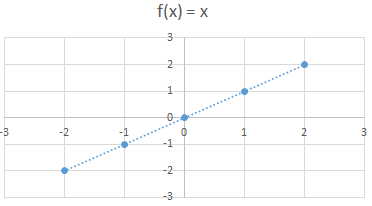
\includegraphics[width=0.7\linewidth]{1_elem_rekenvaardigheden_A/inputs/absValue}
%		\caption{Absolute waarde - voorbeeld 1.}
%		\label{fig:absvalue}
%	\end{figure}	
\end{voorbeeld}

\begin{voorbeeld}
	Zie Figuur \ref{fig:absvalue2}
	\figuurmetlabel[\label{fig:absvalue2}]{width=7cm}{1_elem_rekenvaardigheden_A/inputs/absValue2}{Absolute waarde - voorbeeld 2.}
%	\begin{figure}
%	\centering
%	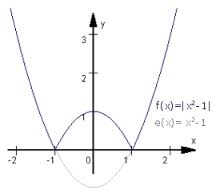
\includegraphics[width=0.7\linewidth]{1_elem_rekenvaardigheden_A/inputs/absValue2}
%	\caption{Absolute waarde - voorbeeld 2.}
%	\label{fig:absvalue2}
%	\end{figure}	
\end{voorbeeld}

\subsection{Sommatie}

Een sommatie is het sommeren of optellen van een groep getallen. 
In de wiskunde wordt een sommatie aangegeven met de griekse hoofdletter sigma: $\sum$ 

\begin{notatie}
Voor getallen $x_m,x_{m+1},\ldots,x_n$ voeren we volgende notatie in
\begin{equation*}
\sum_{i=m}^{n}x_i = x_m + x_{m+1} + x_{m+2} + \ldots + x_{n-2} + x_{n-1} + x_{n}
\end{equation*}	
\end{notatie}

\begin{voorbeeld}
	\begin{equation*}
	\sum_{i=1}^{100}i = 1+2+3+\ldots+100
	\end{equation*}
	De $i$ duidt de index aan. Deze begint te tellen vanaf de ondergrens (in dit voorbeeld 1) tot en met de bovengrens (hier dus 100). Het verhogen gebeurt steeds in stapjes van 1.
	
\end{voorbeeld}

\begin{voorbeeld}
	Soms begint men liever vanaf nul te tellen. In dat geval kan je zelf gemakkelijk de formule en grenzen aanpassen:
	
		\begin{equation*}
	\sum_{i=1}^{100}i = 1+2+3+\ldots+100
	\end{equation*}
	
wordt dan

	\begin{equation*}
\sum_{i=0}^{99} (i+1) = 1+2+3+\ldots+100
\end{equation*}

\end{voorbeeld}

Hieronder worden nog een aantal andere voorbeelden gegeven. Je kan zelf ook eindeloos voorbeelden blijven bedenken.

\begin{voorbeeld}
	\begin{equation*}
	\sum_{i=1}^{10} 4^i = 4^1+4^2+4^3+\ldots+4^{10}
	\end{equation*}
	\begin{equation*}
	\sum_{i=0}^{10} x^{2i} = x^0+x^2+x^4+\ldots+x^{20}
	\end{equation*}
\end{voorbeeld}

In de statistiek wordt vaak gebruik gemaakt van het gemiddelde. Om het gemiddelde $\overline{x}$ van $n$ getallen te berekenen, maak je gebruik van volgende formule:

\begin{equation*}
\overline{x} = \frac{(x_1+x_2+\ldots+x_n)}{n}=\frac{1}{n}(x_1+x_2+\ldots+x_n)
\end{equation*}

Door gebruik te maken van het sommatieteken kan je dit korter noteren:

\begin{equation*}
\overline{x}=\sum_{i=1}^{n}\frac{x_i}{n} = \frac{1}{n} \sum_{i=1}^{n} x_n
\end{equation*}

Hieruit volgt dat je een gemeenschappelijke constante (in dit geval $\frac{1}{n}$) gewoon buiten de eigenlijke sommatie kan plaatsen.



\subsection{Sommatie - voorbeeld}
\begin{minipage}{.25\linewidth}
	\raggedright
	
\includegraphics[width=4cm]{1_elem_rekenvaardigheden_A/inputs/QR_Code_SOMMATIE_module_1}
\end{minipage}
\begin{minipage}{.7\linewidth}
	Zie filmpje MOOC.
\end{minipage}

\subsection{Faculteit}
In dit onderdeel wordt dieper ingegaan op rekenen met faculteiten en indien mogelijk het vereenvoudigen van faculteiten.

\begin{definitie}
	De faculteit van een natuurlijk getal $n$, genoteerd als $n!$ (lees “$n$ faculteit”), is gedefinieerd als het product van de getallen 1 tot en met $n$:
	\begin{equation*}
	n!=n.(n-1)\cdot(n-2)\cdot(n-3)\cdot\ldots\cdot 3\cdot 2\cdot 1
	\end{equation*}
\end{definitie}

De faculteit van $n$ kan je ook met een recursief voorschrift schrijven: $n!=n(n-1)!$

We noemen een voorschrift recursief als er een verband bestaat met vorige resultaten: aangezien $5!=120$ is, geldt
\begin{equation*}
6!=6\cdot 5!=6\cdot 120=720
\end{equation*}
Maar dit recursief gedrag vraagt dat $1!=1\cdot 0!$ Daarom is per definitie gesteld dat:

\begin{definitie}
	0!=1
\end{definitie}

De faculteitsfunctie groeit snel, zelfs sneller dan een exponenti\"ele functie.  $20!$ is een getal van reeds 19 cijfers, terwijl $1000!$ zo'n 2568 cijfers telt.

Het getal $n$ behoort tot de natuurlijke getallen en is dus altijd een positief geheel getal.
Met dit in het achterhoofd kijken we even naar het volgende voorbeeld:

\begin{equation*}
-(3!)=-(3\cdot 2\cdot 1)=-6
\end{equation*}

$(-3)!$ heeft geen betekenis want tussen de haakjes staat een negatief geheel getal en dit behoort niet tot de verzameling van natuurlijke getallen.

\begin{voorbeeld}
	\begin{equation*}
	\frac{6!}{3!}=\frac{6\cdot 5\cdot 4\cdot 3\cdot 2\cdot 1}{3\cdot 2\cdot 1} = 6\cdot 5\cdot 4 = 120
	\end{equation*}
	Let op! Je ziet dus dat je $\frac{6!}{3!}$ niet kan behandelen als een gewone breuk en dat bijgevolg $2!$ een foutief antwoord zou zijn.
\end{voorbeeld}

\begin{voorbeeld}
Een meer algemeen voorbeeld is:
\begin{equation*}
\frac{(n+1)!}{(n-1)!}=\frac{(n+1) \cdot n\cdot (n-1)!}{(n-1)!}=n(n+1)
\end{equation*}
\end{voorbeeld}

Als de faculteitsfunctie $n!$ zo snel toeneemt, dan zal $\frac{1}{n!}$ overeenkomstig ook snel afnemen.

Wiskundig kan je je dan afvragen wat er gebeurt als $n$ oneindig groot wordt. Dit soort vragen zal leiden tot het limietbegrip en notaties als:
\begin{equation*}
\lim\limits_{n \to +\infty} \frac{1}{n!}
\end{equation*}

En wat zou er gebeuren mocht je al deze getallen bij elkaar optellen? Dus waaraan zou volgende som gelijk zijn:

\begin{equation*}
\sum_{=0}^{\infty} \frac{1}{n!} = 1+1+\frac{1}{2!}+\frac{1}{3!}+\ldots=?
\end{equation*}

Dit blijkt het getal $e=2,718\ldots$ te zijn.

Andere toepassingen van de faculteitsfunctie vinden we terug in het vak statistiek en meer bepaald de combinatieleer. Een vaak voorkomende vraag is hier \textquotedblleft op hoeveel verschillende manieren kan je $k$ voorwerpen ordenen?\textquotedblright \  Een voorbeeld: je hebt 2 foto's op je bureau staan. Op hoeveel manieren kan je deze plaatsen? Het antwoord is op $2!=2$ manieren. Met 3 foto's heb je $3!=6$ manieren, en met 10 foto's zijn er al $10!=3628800$ mogelijkheden.

\subsection{Vectoren vs scalairen}
\subsubsection{Wat is een scalair?}
In wetenschap en techniek gebruikt men vaak grootheden die volledig bepaald zijn door \'e\'en re\"eel getal. Degelijke grootheden noemt men scalaire grootheden. Een scalaire grootheid heeft enkel een grootte.

\begin{voorbeeld}
$m=20kg$ (massa), $V=10l$ (volume), $T=35$\textdegree$C$ (temperatuur)
\end{voorbeeld}

\subsubsection{Wat is een vector?}

\begin{definitie}
	We defini\"eren een vector als een grootheid bepaald door een richting, een zin en een grootte.
\end{definitie}

\begin{voorbeeld}
	$\vec{v}=20 m/s$ (snelheid), $\vec{F}=5N$ (kracht), $\vec{E}=20 N/C$ (elektrisch veld)
\end{voorbeeld}

\begin{opmerking}
	\ \\
\begin{itemize}
	\item Een vector is een pijl die twee punten $A$ en $B$ verbindt. Vectoren worden genoteerd door een letter met een pijltje erboven bv. $\vec{v}$. We kunnen ook kiezen om het begin- en eindpunt op te nemen in de notatie. We noteren $\vec{v}=\vec{AB}$.
	\item Een vector $\vec{v}$ wordt volledig bepaald door de grootte, richting en de zin. Twee vectoren zijn dus identiek wanneer hun grootte, hun richting en hun zin dezelfde zijn.
	\item In het algemeen heeft een vector geen positie, men spreekt dan van een \textbf{vrije vector}. Het aangrijpingspunt is niet bepaald. De vrije vectoren behoren tot de verzameling $V$.
	\item De verzameling punten van het vlak noteren we door $\pi$. Kiest men in het vlak $\pi$ een bevoorrecht punt $O$ dan ontstaat het vlak $\pi_O$. Men legt dus de oorsprong  vast in het vlak, en laat alle vector beginnen in de oorsprong. Het punt $P$ in het vlak kunnen we bekijken als het eindpunt van deze vector, namelijk de vector $\vec{OP}=\vec{P}$. Een dergelijke vector noemen we in de wiskunde een \textbf{gebonden} vector, een \textbf{vaste} vector, een \textbf{puntvector} of een \textbf{plaatsvector}. De puntvectoren behoren tot de verzameling $\pi_O$.
	\item De vector $\vec{AA}$ wordt aangeduid met $\vec{O}$ en heeft als lengte 0. Zo een vector noemen we een \textbf{nulvector}. De samenstelling van een vector met een nulvector levert de oorspronkelijke vector op: $\vec{AB}+\vec{O}$. De nulvector is het neutraal element voor de optelling.
	\item Beschouwen we een vector $\vec{AB}$. De vector $\vec{BA}=-\vec{AB}$ met dezelfde richting en grootte, maar met tegengestelde zin wordt de tegengestelde vector genoemd. De samenstelling van een vector met zijn tegengestelde vector levert de nulvector op: $\vec{AB}+\vec{BA}=\vec{O}$.
	\item Een eenheidsvector is een vector met lengte \'e\'en. Eenheidsvectoren worden vooral gebruikt om een richting aan te geven. Een vector met willekeurige niet-nulle norm kan worden gedeeld door zijn norm om zo een eenheidsvector te cre\"eren. Dit proces staat bekend als het normaliseren van een vector. Een eenheidsvector wordt vaak aangeduid met een hoedje, zoals in $\hat{a}$  of ook door $\vec{e_1}$ (of $\vec{1_x}$ als het over de eenheidsvector volgens de $x$-as gaat).
	\begin{equation*}
	\hat{a} = \frac{\vec{a}}{||\vec{a}||}
	\end{equation*}
	\item De lengte of de norm van een vector $\vec{AB}$ of $\vec{v}$ noteert men door $||\vec{AB}||$ of $||\vec{v}||$.
\end{itemize}	
\end{opmerking}

\subsubsection{Bewerkingen met vectoren}

\emph{De optelling}

\begin{definitie}
De som van twee vectoren is opnieuw een vector: $\vec{v_1}+\vec{v_2}=\vec{v}$

Het verschil van twee vectoren is opnieuw een vector. $\vec{v_1}-\vec{v_2}=\vec{v_1}+(-\vec{v_2})=\vec{v}$
\end{definitie}

\begin{opmerking}
	Let op! $||\vec{v_1}||+||\vec{v_2}|| \ne ||\vec{v}||$
\end{opmerking}

Het samenstellen van twee vectoren gebeurt volgens de \textbf{parallellogramregel}, zie Figuur \ref{fig:som_par}. Wanneer we twee vectoren $\vec{v_1}$ en $\vec{v_2}$ (met een verschillende richting) willen optellen, dan construeren we een parallellogram. We plaatsen $\vec{v_1}$ en $\vec{v_2}$ zodat hun aangrijpingspunt samenvalt. De som $\vec{v_1}+\vec{v_2}$ wordt dan gegeven door de vector met het aangrijpingspunt en eindpunt het overstaand hoekpunt van de parallellogram.

\figuurmetlabel[\label{fig:som_par}]{width=7cm}{1_elem_rekenvaardigheden_A/inputs/parRegelSom}{Parallellogramregel voor het bepalen van de som van 2 vectoren.}

Deze parallellogram constructie kan ook gebruikt worden voor het omgekeerde proces, namelijk het \textbf{ontbinden van een vector in 2 (of meerdere) componenten (dit zijn scalairen)}, elk volgens een bepaalde richting. Vaak wordt dan een gegeven vector ontbonden in een component volgens de $x$-as en een component volgens de $y$-as.

\figuurmetlabel[\label{fig:kopstaartsom_par}]{width=7cm}{1_elem_rekenvaardigheden_A/inputs/kopstaart}{Kopstaartregel voor het bepalen van de som van 2 vectoren.}

Een andere manier om twee vectoren op te tellen, is deze kop aan staart te leggen, zie Figuur \ref{fig:kopstaart}. We plaatsen de vector $\vec{v_2}$ zodat zijn beginpunt samenvalt met het eindpunt van de vector $\vec{v_1}$. De som  wordt dan gegeven door de vector wijzend van het beginpunt van $\vec{v_1}$ naar het eindpunt van $\vec{v_2}$. Deze regel noemen we de \textbf{driehoeksregel} of de \textbf{kopstaartregel}.

\emph{De vermenigvuldiging van een vector met een scalair}

\begin{definitie}
	Wanneer men een vector $\vec{v}$ vermenigvuldigt met een scalair $k$, krijgt men de nieuwe vector $k\vec{v}$. 
	
	De grootte van deze nieuwe vector is $k||\vec{v}||$.
	
	De richting verandert niet, terwijl de zin omdraait als $k<0$ (lees “als $k$ negatief is”).
\end{definitie}

\begin{opmerking}
	Let op! een scalaire vermenigvuldiging mag je niet verwarren met het scalair product (zie verder)
\end{opmerking}

\emph{De vermenigvuldiging van twee vectoren}

\begin{definitie}
	\ \\
\begin{enumerate}
	\item het scalair product of inwendig product:
	\begin{equation*}
	\vec{v_1} \cdot \vec{v_2} = ||\vec{v_1}|| \cdot  ||\vec{v_2}|| \cdot \cos \theta = \text{getal}
	\end{equation*}
	Hierbij is $\theta$ de hoek tussen de 2 vectoren. Het scalair product is dus maximaal als beide vectoren in dezelfde richting wijzen (met andere woorden parallel zijn). En anderzijds is het scalair product nul als beide vectoren loodrecht op elkaar staan.

	\item het vectorieel product, kruisproduct of uitwendig product:
	\begin{equation*}
	\vec{v_1} \times \vec{v_2} = \begin{vmatrix}
	\vec{e_1} & \vec{e_2} & \vec{e_3} \\
	a_1 & a_2 & a_3 \\
	b_1 & b_2 & b_3 
	\end{vmatrix} = \text{vector}
	\end{equation*} 
\end{enumerate}
\end{definitie}
De eigenschappen van de nieuwe vector zijn:

\begin{enumerate}
	\item Over de richting van $\vec{a} \times \vec{b}$: het staat loodrecht op $\vec{a}$ en $\vec{b}$.
	\item Over de zin van $\vec{a} \times \vec{b}$: $\vec{a}$, $\vec{b}$  en $\vec{a} \times \vec{b}$ vormen een rechtshandig assenstelsel.
	\item De norm van $\vec{a} \times \vec{b}$ is $||\vec{a} \times \vec{b}||=||\vec{a}||\cdot||\vec{b}||\cdot \sin \theta$, waarin $\theta$ de hoek is tussen $\vec{a}$ en $\vec{b}$.
\end{enumerate}
Het vectorieel product is dus maximaal als beide vectoren loodrecht op elkaar staan. En anderzijds is het vectorieel product nul als beide vectoren evenwijdig zijn (en dus dezelfde richting hebben).

\subsection{Ontbinden van een vector - voorbeeld}
\begin{minipage}{.25\linewidth}
	\raggedright
	
\includegraphics[width=4cm]{1_elem_rekenvaardigheden_A/inputs/QR_Code_ONTBINDEN_module_1}
\end{minipage}
\begin{minipage}{.7\linewidth}
	Zie filmpje MOOC.
\end{minipage}

\subsection{Test - wiskundige notaties}
TODO

\section{Bewerkingen}

\subsection{Volgorde van bewerkingen}
Om een opgave juist te kunnen oplossen, is het noodzakelijk om de volgorde van de bewerkingen te respecteren:

\begin{enumerate}
	\item \textbf{H}aakjes
	\item \textbf{M}achten en worteltrekken
	\item \textbf{W}issel van teken
	\item \textbf{V}ermenigvuldigen en \textbf{d}elen (dezelfde prioriteit)
	\item \textbf{O}ptellen en \textbf{a}ftrekken (dezelfde prioriteit)
\end{enumerate}

Let op! Haakjes staan voor deelopgaven die je eerst moet maken, hierop moet je inzoomen.

\emph{Opmerkingen}
\begin{itemize}
	\item Bewerkingen met dezelfde prioriteit worden van links naar rechts uitgevoerd.
	\item Een ezelsbruggetje om dit te onthouden: \textbf{H}oe \textbf{M}oeten \textbf{W}ij \textbf{V}an \textbf{D}e \textbf{O}nvoldoendes \textbf{A}fkomen?
	\item Machtsverheffen gaat voor op tekenwisseling: als je $-5^2$ moet uitrekenen, doe je eerst $5^2=25$ en daarna pas je op het resultaat de tekenwisseling toe zodat het antwoord $-25$ wordt.
	\item Bedoel je echter het kwadraat van $-5$ dan noteer je $(-5)^2=(-5).(-5)=25$
\end{itemize}

\subsection{Volgorde van bewerkingen - voorbeeld 1}
Zie filmpje MOOC.

\subsection{Volgorde van bewerkingen - voorbeeld 2}
Zie filmpje MOOC.

\subsection{Rekenen met machten of exponenten}
\emph{Wat is een macht?}
De vermenigvuldiging is ingevoerd om de schrijfwijze bij een optelling te vereenvoudigen. Immers:
\begin{equation*}
\underbrace{4+4+4+4+4+4}_{\text{6 maal}}
\end{equation*}
was vervelend om te schrijven. Omdat de 4 zesmaal voorkomt, werd dit $6 \cdot 4$.

Later werd er dan ook gedefinieerd wat het betekende om kommagetallen met mekaar te vermenigvuldigen.

Machten zijn ingevoerd om volgende schrijfwijzes eenvoudiger te maken:
\begin{equation*}
\underbrace{4 \cdot 4\cdot4\cdot4\cdot4\cdot4}_{\text{6 maal}}
\end{equation*}
In plaats van een som van dezelfde getallen, hebben we nu een product van dezelfde getallen.

Verkort geschreven wordt dit: $4^6$

Een macht bestaat uit twee delen: een exponent, hier $6$ en een grondtal, hier $4$.

Het grondtal mag (mits enkele uitzonderingen) elk re\"eel getal zijn. De exponent mag eigenlijk (ook weer met enkele uitzonderingen) elk re\"eel getal zijn. Om de volgorde van bewerkingen uit te leggen, gebruiken we in dit hoofdstuk enkel natuurlijke (gehele) exponenten.

\begin{voorbeeld}
	\begin{equation*}
	12+3^2 \cdot 4 : 2 - 8 : 4 + 3 - 5^2
	\end{equation*}
	Hoe pakken we dit nu aan? We zien dat er enkele machten in staan, dus die rekenen we eerst uit. Vervolgens rekenen we alle vermenigvuldigingen en delingen uit, van links naar rechts. Dan doen we alle optellingen en aftrekkingen, van links naar rechts.
	\begin{equation*}
	\begin{array}{lllr}
	12+\underbrace{3^2}_{9} \cdot 4 : 2 - 8 : 4 + 3 - \underbrace{5^2}_{25} &=& 12+ \underbrace{9 \cdot 4}_{36} : 2 - \underbrace{8 : 4}_{2} + 3 - 25 & \text{vermenigvuldigen en delen} \\
	&=& 12+ \underbrace{36 : 2}_{18} - 2 + 3 - 25 & \text{vermenigvuldigen en delen} \\
	&=& \underbrace{12+18} _{30} - 2 + 3 - 25 & \text{optellen en aftrekken} \\
	&=& \underbrace{30 - 2}_{28} + 3 - 25 & \text{optellen en aftrekken} \\
	&=& \underbrace{28+3}_{31} - 25 & \text{optellen en aftrekken} \\
	&=& 31 - 25 & \text{optellen en aftrekken} \\
	&=& 6 &  \\
	\end{array}
	\end{equation*}
\end{voorbeeld}


\subsection{Werken met haakjes}
\emph{Wat als er haakjes staan?}

Haakjes zijn nuttig om aan te duiden dat de bewerking ertussen eerst moet gebeuren. Haakjes zullen dus voorrang hebben op alles.

\fbox{\begin{minipage}{\linewidth}
	Onthoud \\
	
	Los eerst alles tussen de haakjes op!	
	\end{minipage}}

Haken symboliseren in feite een deelopgave. Ze verplichten je eerst die deelopgave op te lossen, vooraleer je de grote oplossing mag starten.


\begin{voorbeeld}
\begin{equation*}
6 \cdot (4+5) = 6 \cdot 9 = 54
\end{equation*}	
	
In deze opgave is $(4 + 5)$ de deelopgave, dus die los je eerst op en je vult het resultaat in. 
Dan ga je gewoon verder met de rest van de opgave.

Even vergelijken wat er gebeurt als er geen haken staan, dus dan moet je eerst de vermenigvuldiging uitwerken:

\begin{equation*}
6 \cdot 4+5 = 24+5=29
\end{equation*}	

Iets totaal anders!

Let op: $6 \cdot (4+5) \ne 6\cdot 4+5$

\end{voorbeeld}

\begin{voorbeeld}

\begin{equation*}
\begin{array}{ccrl}
20 : 4 \cdot 5 &=& 20:20 =1 & \text{is fout,} \\
20 : 4 \cdot 5 &=& 5 \cdot 5 =25 & \text{is juist.}
\end{array}
\end{equation*}
	
Dit soort fouten kan je voorkomen door (zelf) haakjes te gebruiken:

\begin{equation*}
(20 : 4) \cdot 5 = 5 \cdot 5 = 25
\end{equation*}

Een andere manier om dit soort problemen te omzeilen is door “delen door 4” te vervangen door “vermenigvuldigen met een vierde” en vervolgens van links naar rechts te rekenen:

\begin{equation*}
20 : 4 \cdot 5 = 20 \cdot \frac{1}{4} \cdot 5 = 25
\end{equation*}

Dit geldt ook voor de optelling en de aftrekking:

\begin{equation*}
\begin{array}{ccrl}
5-3+1 &=& 5-4 =1 & \text{is fout,} \\
5-3+1 &=& 2+1=3 & \text{is juist.}
\end{array}
\end{equation*}

Dit soort fouten kan je voorkomen door (zelf) haakjes te gebruiken:

\begin{equation*}
(5-3)+1 = 2+1=3 
\end{equation*}

Een andere manier is om dit soort problemen te omzeilen is door “aftrekken van plus 3” te vervangen door “optellen met min drie” en vervolgens van links naar rechts te rekenen:

\begin{equation*}
5-3+1 = 5+(-3)+1=3 
\end{equation*}

\end{voorbeeld}

\emph{Wat als er meerdere haakjes zijn?}

\fbox{\begin{minipage}{\linewidth}
Soms kunnen er meerdere haakjes voorkomen. Er geldt dan de volgende regel: Bij meerdere haakjes, werk je eerst de binnenste uit, en dan werk je naar buiten. 

Wat is er eigenlijk aan de hand? In de deelopgave van de buitenste haakjes staan er nog meer haakjes. Dit is in feite een deelopgave in een deelopgave.

\begin{enumerate}
	\item Je start met die binnenste deelopgave.
	\item Je vult de uitkomst van die deelopgave in.
	\item Je gaat verder met de volgende deelopgave.
	\item Je vult dit weer in.
	\item Enzoverder!
\end{enumerate}
	\end{minipage}
}

\begin{voorbeeld}
\begin{equation*}
((3+6)-4^2)\cdot 2
\end{equation*}
Dit voorbeeld heeft verschillende haken (deelopgaven). Je ziet de buitenste haken. Daar is de deelopgave dus:
\begin{equation*}
((3+6)-4^2)
\end{equation*}
Binnen deze deelopgave staan nieuwe haken, dus die moet je weer eerst uitrekenen, we starten dus met het uitrekenen van de binnenste haken:
\begin{equation*}
\begin{array}{cclr}
\left( \underbrace{(3+6)}_{9}-4^2\right)\cdot 2 &=& \left( 9-\underbrace{4^2}_{16}\right)\cdot 2 & \text{machten binnen de haakjes} \\
&=& \underbrace{(9-16)}_{-7}\cdot 2 & \text{haken} \\
&=& -7 \cdot 2 & \text{min maal plus is min} \\
&=& -14
\end{array}
\end{equation*}
Let dus goed op in dit voorbeeld. Je moet haken altijd eerst uitrekenen, van binnen naar buiten.

Je moet een deelopgave (die binnen de haken staat) zelf behandelen als een opgave en dus de volgorde van bewerkingen daarbinnen toepassen.

\end{voorbeeld}
\subsection{Begrippen tegengestelde en omgekeerde van een getal}

\subsubsection{Tegengestelde}

Het \emph{tegengestelde} van een getal $n$ is het getal dat opgeteld
bij $n$, nul oplevert. Het tegengestelde van n wordt genoteerd met
$-n$. Het tegengestelde van een getal heeft dus dezelfde absolute
waarde als het gegeven getal maar met een tegengesteld teken. De som
van een getal met zijn tegengestelde is dus steeds 0: $n+(-n)=0$.

\noindent Zo is het tegengestelde van 12 gelijk aan \textminus 12
omdat 12 + (\textminus 12) = 0, en het tegengestelde van $-\sqrt{3}$
is $\sqrt{3}$ omdat $-\sqrt{3}+\sqrt{3}=0$.

\medskip{}


\noindent Het tegengestelde van nul is nul. Dit is het enige getal
waarvan het tegengestelde gelijk is aan zichzelf. 

\noindent We zeggen dat 0 het \emph{neutraal element} is met betrekking
tot optellen.

\noindent (In de abstracte algebra is het tegengestelde het inverse
element voor een bewerking die met een plusteken genoteerd wordt).

\bigskip{}

\subsubsection{Omgekeerde}

\noindent Het \emph{omgekeerde} of de \emph{reciproque} (vaker: de
reciproke) van een getal of grootheid is 1 gedeeld door dat getal
of die grootheid. Het omgekeerde van een breuk ontstaat door teller
en noemer te verwisselen. Het omgekeerde van 7 is 1/7 en het omgekeerde
van 2/3 is 3/2. Passen we dit toe op enkele grootheden: de hertz is
het omgekeerde van de seconde: 1 Hz = 1/s en de siemens is het omgekeerde
van de ohm: 1 S = 1/$\Omega$.

\noindent Het product van een getal met zijn omgekeerde levert 1 op:
${\displaystyle n.\frac{1}{n}=1}$. 

\noindent We zeggen dat 1 het \emph{neutraal element} is voor de vermenigvuldiging.
We zien ook dat nul geen omgekeerde heeft.

\noindent (In de abstracte algebra is het omgekeerde het inverse element
voor een bewerking die met een vermenigvuldigingsteken genoteerd wordt).

\medskip{}


\noindent Een interessante toepassing van het omgekeerde vinden we
bij de deling waarbij de deler een breuk is. De deling kan dan ook
uitgevoerd worden door het deeltal te vermenigvuldigingen met het
omgekeerde van de deler. 

\noindent Populair gezegd: delen door een breuk is vermenigvuldigen
met het omgekeerde.

\noindent Voorbeeld: $5:1/3=5\times3=15$ 


\subsection{Rekenen met wortels}
TODO


\subsection{Rekenen met breuken}
TODO

\subsection{Rekenen met logaritmen}
TODO

\subsection{Algebra: het rekenen met letters}


\subsubsection{Gebruik van letters in de wiskunde}

De algebra is de kunst van het rekenen met letters. Die letters stellen
meestal getallen voor, en met getallen weet je hoe je kan rekenen:
optellen, aftrekken, vermenigvuldigen en delen. Bij algebra voeren
we dat soort operaties ook uit, alleen gebruiken we daarbij niet alleen
getallen, maar ook \emph{variabelen}. Dat zijn als het ware 'dingen'
waarvan we de waarde (nog) niet kennen of waarbij zo'n 'ding' meerdere
waarden kan aannemen. Voor de variabelen gebruiken we letters.

\noindent In de algebra worden vervolgens allerlei verbanden en structuren
onderzocht. Welke regels en eigenschappen gelden er, wat mag wel en
wat mag niet? Verzamelingen spelen hierbij een grote rol, maar ook
afbeeldingen. Door gebruik te maken van variabelen, vergelijkingen,
en dergelijke meer is het mogelijk 'algemene' uitspraken te doen over
verzamelingen en operaties. Bekende eigenschappen van rekenen met
getallen zijn de commutatieve eigenschap en de distributieve eigenschap.

\medskip{}

Voorbeeld: In het algemeen geldt voor het optellen en vermenigvuldigen
van $a$ en $b$ (natuurlijke getallen) dat:

\begin{equation*}
a + b = b + a \text{ en } a \times{} b = b \times{} a
\end{equation*}

Dat lijkt vanzelfsprekend, maar dat is het niet. Bij de operatie delen
geldt het bijvoorbeeld niet! ($12:4$ is niet hetzelfde als $4:12$)

\medskip{}

Een andere bekende eigenschap is de distributiviteit:

\begin{equation*}
a \texttimes{} (b + c) = a \texttimes{} b + a \texttimes{} c
\end{equation*}

Dat gebruiken we heel vaak, maar mag dat zomaar, wanneer wel, wanneer
niet?

Geldt dit bijvoorbeeld?

\begin{equation*}
a + (b \times{} c) = (a + b) \times{} (a + c) ???
\end{equation*}

\medskip{}


\noindent Met variabelen kunnen we ook \emph{formules} opstellen.
Stel dat we de straal van een cirkel voorstellen door de letter $r$.
Dan is de $\mathrm{omtrek}=2\pi r$ en de $\mathrm{oppervlakte}=\pi r^{2}$.
Nu kunnen we voor eender welke cirkel zijn omtrek en oppervlakte berekenen
door de waarde van $r$ te vervangen (we zeggen te \emph{substitueren})
door een getal.

\medskip{}


\noindent Een \emph{uitdrukking} is een geheel van termen bestaande
uit getallen, variabelen, bewerkingstekens (zoals $+$, $-$, $x$, $:$) en andere
wiskundige tekens (zoals haakjes): $2\pi r$, $3-8$, $2x+5$, ...

\noindent Vervolgens kunnen we twee uitdrukkingen aan elkaar gelijk
stellen. We spreken dan van een \emph{vergelijking}. Vergelijkingen
kunnen vaak worden afgeleid uit een stukje tekst (de klassieke vraagstukjes).
Als een vergelijking een variabele bevat, dan kunnen we trachten de
waarde (of alle waarden) van de variabele te vinden waardoor er een
ware bewering ontstaat als we de variabele vervangen door de gevonden
waarde(n). Dit wordt \emph{oplossen van de vergelijking} genoemd.
De waarde van de variabele heet in dit geval \emph{de wortel} of \emph{de
oplossing} van de vergelijking.

\noindent Een formule kan (en mag) meerdere variabelen en onbekenden
bevatten. \medskip{}


\uline{Voorbeeld 1}:

De oppervlakte van een rechthoek is $b.h$ waarbij $b$ de basis is,
en $h$ de hoogte.

Als je nu gegeven krijgt dat $b$ gelijk is aan 4 en $h$ gelijk is
aan 2 (we gebruiken even geen eenheden ter vereenvoudiging), dan kan
je de oppervlakte berekenen door de letters te substitueren, door
ze te vervangen door de echte waarden of echte getallen:

\begin{equation*}
\mathrm{oppervlakte}=b\cdot h=(4)\cdot(2)=8
\end{equation*}

Hoewel het hier niet echt nodig was, hebben we toch de gesubstitueerde
getallen tussen haken gezet. Je doet dit om aan te duiden dat je de
letter in zijn geheel vervangt door het getal. Bij moeilijke formules
maakt dit wel degelijk veel uit! Stel, je wil de oppervlakte van een
andere rechthoek berekenen, en je hebt gegeven dat de hoogte 2 meer
moet zijn dan de basis, of met andere woorden, $h=b+2$. Over de basis
weet je nog niets. Je kan dus enkel $h$ vervangen:

\begin{equation*}
\mathrm{oppervlakte}=b\cdot h=b\cdot(b+2)
\end{equation*}

Je ziet dus dat de letter $h$ volledig vervangen is door $b+2$,
gesymboliseerd door de haakjes.

\medskip{}


\uline{Voorbeeld 2}:

Ik heb een pot verf waarmee een oppervlakte van $5m^2$
kan geschilderd worden. Hoeveel ronde tafeltjes kan ik hiermee een
likje verf geven? De diameter van de tafeltjes is $1~m$.

Oplossing: 

We zoeken het aantal tafeltjes die volledig geschilderd kunnen worden.
Stel deze onbekende variabele voor door bijvoorbeeld $x$ (gevraagd).

We hebben voldoende verf om $~5~m^2$
te schilderen (gegeven).

De diameter $d$ van een tafeltje is 1 meter: $d=1~m$ (gegeven).

De straal $r$ van een cirkel is de helft van de diameter: $2r=d$

zodat de oppervlakte $s$ van 1 tafeltje gelijk is aan: $s=\pi r^{2}=\pi\left(\frac{d}{2}\right)^{2}=\frac{\pi d^{2}}{4}=\frac{\pi(1)^{2}}{4}=0,79~m^2$

We stellen de vergelijking op: $5=x.s$ 

en lossen deze tenslotte op naar de onbekende variabele: $x=\frac{5}{s}=\frac{5}{0,79}=6,37$

Besluit: we kunnen 6 tafeltjes schilderen (en dan blijft er nog een
klein beetje verf over).


\subsubsection{Manier van rekenen}

\begin{itemize}
	\item{Notaties}
	\begin{itemize}
		\item In het rekenen met letters wordt het puntje van de vermenigvuldiging
		vaak niet geschreven. In plaats van $a\cdot b\cdot c$ schrijf je
		$abc$. Of, in plaats van $2\cdot b$ schrijf je $2b$. Het puntje
		schrijven is niet fout, maar hoeft niet.
		\item Letters schrijf je achteraan in een uitdrukking, dus $b\cdot2\cdot c$
		schrijf je best als $2bc$. (Dit mag, want in een product mag je factoren
		van plaats verwisselen.)
		\item Vaak worden de letters die voorkomen ook in alfabetische volgorde
		geschreven. Bijvoorbeeld $yxz$ schrijf je beter als $xyz$. 
	\end{itemize}
	\noindent Deze notaties maken het meestal gemakkelijker om verder
	te rekenen, en als je je aan deze manier van schrijven houdt, ziet
	alles er meer netjes uit. Het is niet absoluut verplicht om te doen,
	maar wel aan te raden.
	
	
	\item{Eentermen en veeltermen}
	
	Een eenterm is een uitdrukking die uit 1 term bestaat, een veelterm
	bestaat uit meerdere termen, logisch toch? I.p.v. een veelterm spreken
	we ook over een polynoom.
	
	\textbullet{} $a$ en $4abcx$ zijn eentermen
	
	\textbullet{} $x^{2}+3x+1$ en $b-x$ zijn veeltermen
	
	
	\item{Som en verschil}
	
	Je kan de som of het verschil van eentermen maken, maar enkel als
	de letters of lettercombinatie in de eenterm gelijk is. Lijkt een
	cryptische regel, maar dat is het niet. 
	
	\noindent Bijvoorbeeld:
	
	\textbullet{} $a+3a=4a$ Dit gaat perfect, want de letters zijn gelijk.
	
	\textbullet{} $a+2b=?$ Dit gaat niet, $a$ en $b$ zijn verschillende
	letters. 
	
	\textbullet{} $2ab+bc=?$ Dit gaat niet want $ab$ en $bc$ zijn verschillende
	lettercombinaties. 
	
	\textbullet{} $3ab-ab=2ab$ Dit gaat perfect, want de lettercombinaties
	zijn gelijk.
	
	\textbullet{} $ab+ba=ab+ab=2ab$ Ook dit gaat, al is het met een omweg.
	Door te sorteren zie je dat de lettercombinaties gelijk zijn.
	\begin{itemize}
		\item $a+a^{2}=?$ Dit gaat niet, want de lettercombinaties zijn niet gelijk,
		eentje is een $a$ en de andere is $a^{2}$.
	\end{itemize}
	Let dus goed op bij het optellen van letters of combinaties, en sorteer
	de letters om gelijkaardige combinaties te zien. 
	
	\noindent Het optellen van veeltermen is een uitbreiding van deze
	regel. Gelijksoortige eentermen (dus met dezelfde lettercombinaties)
	tel je op: 
	\begin{itemize}
		\item \noindent $(3x+y)+(4x+z)=7x+y+z$ Enkel de eentermen van de $x$ kan
		je optellen, de rest moet je laten staan. 
		\item \noindent $(3x+y)-(a+b)=3x+y-a-b$ Jammer, hier kan je niets optellen.
	\end{itemize}
	
	\item{Producten}
	
	Producten van verschillende letters vorm je door de letters achter
	elkaar te schrijven. De bijhorende getallen vermenigvuldig je ook,
	en plaats je voorop. 
	
	\noindent Voor eentermen is dit:
	
	\textbullet{} $a\cdot b\cdot x=abx$ 
	
	\textbullet{} $x\cdot2a\cdot2b=4abx$ \medskip{}
	
	
	\noindent Als de letters gelijk zijn, kan je machten vormen. Je gebruikt
	hier eigenlijk de rekenregel: ``machten met hetzelfde grondtal vermenigvuldigen
	is de exponenten optellen''.
	\begin{itemize}
		\item \noindent $a\cdot a=a^{2}$
		\item \noindent $x^{2}\cdot x^{3}=x^{2+3}=x^{5}$
		\item \noindent $ab\cdot ab=(ab)^{2}=a^{2}\cdot b^{2}=a^{2}b^{2}$
	\end{itemize}
	\noindent Veeltermen vermenigvuldigen is lastiger, maar maakt gebruik
	van rekenregels die je al kent. De belangrijkste is de distributiviteit.
	Op die manier herleid je het probleem naar het product van eentermen:
	\begin{equation*}
	x\cdot(a+b)=x\cdot a+x\cdot b=ax+bx
	\end{equation*}
%	\begin{itemize}
%		\item \noindent $x\cdot(a+b)=x\cdot a+x\cdot b=ax+bx$
%	\end{itemize}
	\noindent Iets complexer: nog enkele voorbeelden:
	
	\begin{math}
	\begin{array}{ccc|r}
	(a+2x)\cdot(3x) & = & a\cdot(3x)+(2x)\cdot(3x) & \text{ distributiviteit}\\
	& = & 3ax+6x^{2} & \text{uitrekenen en ordenen}\\
	& & & \\
	(a+b)\cdot(a+b) & = & a\cdot a+b\cdot a+a\cdot b+b\cdot b &  \text{distributiviteit}\\
	& = & a^{2}+ba+ab+b^{2} &  \text{uitrekenen}\\
	& = & a^{2}+2ab+b^{2} &  \text{ordenen en optellen}\\
	& &  & \\
	(a+b)\cdot(x+y) & = & a\cdot x+a\cdot y+b\cdot x+b\cdot y=ax+ay+bx+by\\
	\end{array}
	\end{math}
	

	\noindent In module {*}{*}{*}{*} gaan we kijken naar de omgekeerde
	bewerkingen: ontbinden in factoren (afzonderen van eentermen en veeltermen),
	en merkwaardige producten.
	
	
	\item{Quoti\"enten}
	
	Quoti\"enten, en dus daarmee samenhorend breuken, bereken je vaak door
	vereenvoudigingen. Je doet een vereenvoudiging net op dezelfde manier
	als bij het vereenvoudigen van een breuk met gewone getallen:
	
	\begin{eqnarray*}
		\frac{6}{15} & = & \frac{2.3}{3.5} = \frac{2}{5}\\
		\frac{ab}{bc} & = & \frac{a}{c} \\
	\end{eqnarray*}
	

	\noindent Als er in de teller een letter staat die ook in de noemer
	staat, kan je de breuk vereenvoudigen. Maar de volgende breuk kan
	je NIET vereenvoudigen:
	
	\begin{equation*}
		{\displaystyle \frac{ab}{bc+1}}
	\end{equation*}
	
	\noindent In de noemer staat immers niet bij elke term een $b$, dus
	is vereenvoudiging hier niet mogelijk. Wat je echter wel kan (en mag
	doen) is zowel in teller als noemer de letter $b$ buiten de haakjes
	brengen; daarna kan je $b$ schrappen, maar of je daarmee de breuk
	vereenvoudigd hebt, laten we in het midden. De variabele $b$ mag
	nu immers niet meer nul worden.
	
	\begin{equation*}
	{\displaystyle \frac{ab}{bc+1}={\displaystyle \frac{ab}{b(c+\frac{1}{b})}=\frac{a}{c+\frac{1}{b}}}}
	\end{equation*}
	
	\medskip{}
	
	
	\noindent Het gebruik van rekenregels heb je echt nodig bij machten:
	
	\noindent ${\displaystyle \frac{a^{3}}{a^{2}}=a^{3-2}=a^{1}=a}$
	
	\noindent \medskip{}
	
	
	\noindent Nog een voorbeeld:
	
	\begin{math}
	\begin{array}{ccc|r}
	{\displaystyle \frac{p\sqrt{p}}{p^{2}}} & = & {\displaystyle \frac{p.p^{\frac{1}{2}}}{p^{2}}} &   \text{vierkantswortel omzetten in macht}\\
	& = & {\displaystyle \frac{p^{1+\frac{1}{2}}}{p^{2}}} &  \text{product van machten met gelijk grondtal is exponenten optellen}\\
	& = & {\displaystyle \frac{p^{\frac{3}{2}}}{p^{2}}} &  \\
	& = & {\displaystyle p^{\frac{3}{2}-2}} &  \text{quoti\"ent van machten met gelijk grondtal is exponenten aftrekken}\\
	& = & {\displaystyle p^{-\frac{1}{2}}} &  \text{Verder dan dit kan je de opgave niet vereenvoudigen.}\\
	\end{array}
	\end{math}
	
	\noindent Als je iets meer ervaring hebt: ${\displaystyle \frac{p\sqrt{p}}{p^{2}}=p^{1+\frac{1}{2}-2}={\displaystyle p^{-\frac{1}{2}}}}$.
	
\end{itemize}


\subsubsection{Voorbeelden}

\noindent Rekenen met letters kan dan wel op dezelfde manier gaan
zoals rekenen met getallen, toch is er vaak een moeilijkheid bij vereenvoudigingen
en dergelijke. Vandaar dat we enkele voorbeelden bekijken.

\begin{itemize}
	\item{Breuken optellen en aftrekken}
	
	\noindent Net zoals bij de gewone breuken, is de sleutel hier het
	op dezelfde noemer brengen van de breuken:
	
	\begin{equation*}
	{\displaystyle \frac{4}{a}+\frac{7}{a}=\frac{11}{a}}
	\end{equation*}
	
	\noindent Volgend voorbeeld is iets lastiger:
	
	\begin{equation*}
		{\displaystyle \frac{a}{b}+\frac{c}{d}}
	\end{equation*}
	
	\noindent Je zoekt hier een gelijke noemer. Omdat de noemers niets
	met mekaar te maken hebben, neem je gewoon het product van de noemers
	als gemeenschappelijke noemer, namelijk $b\cdot d$. Dat zou je ook
	doen als je de som $\frac{1}{7}+\frac{2}{3}$ zou moeten oplossen,
	dan zou je ook als gemeenschappelijke noemer $3\cdot7=21$ kiezen.
	
	\begin{equation*}
		{\displaystyle \frac{a}{b}+\frac{c}{d}=\frac{ad}{bd}+\frac{cb}{bd}=\frac{ad+bc}{bd}}
	\end{equation*}
		
	\noindent Een iets moeilijker voorbeeld:
	
	\begin{eqnarray*}
		{\displaystyle \frac{y}{x}+\frac{y}{x+1}} & = & {\displaystyle \frac{y.(x+1)}{x.(x+1)}+\frac{y.x}{(x+1).x}} \\
		& = & {\displaystyle \frac{xy+y}{x.(x+1)}+\frac{xy}{(x+1).x}} \\
		& = & {\displaystyle \frac{xy+y+xy}{x.(x+1)}} \\
		& = & {\displaystyle \frac{2xy+y}{x(x+1)}} \\
		& = & {\displaystyle \frac{2xy+y}{x^{2}+x}} 
	\end{eqnarray*}
	We werken hier ook de noemer uit.
	
	
	\noindent \medskip{}
	Nog een laatste voorbeeld:
	
	\begin{equation*}
	{\displaystyle \frac{x+3+a}{a+1}-\frac{2x+5-b}{2a+2}}
	\end{equation*}
	
	\noindent In dit voorbeeld is de gemeenschappelijke noemer gelijk
	aan $2a+2$, en niet meteen het product van de twee noemers! Immers,
	de twee noemers hebben een gemeenschappelijk factor, namelijk $a+1$.
	Daar moet je gebruik van maken. Concreet betekent dit dat we de eerste
	breuk in teller en noemer moeten vermenigvuldigen met 2, en de tweede
	noemer kunnen we gewoon laten staan:
	
	\begin{math}
	\begin{array}{ccl|r}
	{\displaystyle \frac{x+3+a}{a+1}-\frac{2x+5-b}{2a+2}} & = & {\displaystyle \frac{(x+3+a).2}{(a+1).2}-\frac{2x+5-b}{2a+2}}  & \text{op gelijke noemer zetten}\\
	& = & {\displaystyle \frac{2x+6+2a}{2a+2}-\frac{2x+5-b}{2a+2}} &\text{uitrekenen}\\
	& = & {\displaystyle \frac{2x+6+2a-(2x+5-b)}{2a+2}} & \text{ verschil van tellers, vergeet geen haken!}\\
	& = & {\displaystyle \frac{2x+6+2a-2x-5+b}{2a+2}} & \text{minteken verdelen over termen}\\
	& = & {\displaystyle \frac{1+2a+b}{2a+2}} & \text{gelijkaardige termen optellen}\\
	\end{array}
	\end{math}
	
	
	\item{Breuken vermenigvuldigen en delen}
	
	Breuken vermenigvuldigen en delen is eenvoudiger dan optellen en aftrekken;
	opnieuw gebruik je dezelfde rekenregels als voordien. 
	
	\noindent Vermenigvuldigen van breuken is tellers met tellers en noemers
	met noemers vermenigvuldigen:
	
	\begin{equation*}
		{\displaystyle \frac{a}{b}\cdot\frac{2}{x}=\frac{a.2}{b.x}=\frac{2a}{bx}} 
	\end{equation*}
	
	\noindent Een getal delen door een breuk is vermenigvuldigen met het
	omgekeerde van die breuk:
	
	\begin{equation*}
		{\displaystyle \frac{a}{b}:\frac{2}{x}=\frac{a}{b}.\frac{x}{2}=\frac{a.x}{b.2}=\frac{ax}{2b}}
	\end{equation*}	
	
	\noindent Ietsje moeilijker:
	
	\begin{math}
		\centering
	\begin{array}{ccc|r}
	{\displaystyle \frac{a+b}{c+d}.\frac{x+1}{y+1}} & = & {\displaystyle \frac{(a+b)}{(c+d)}.\frac{(x+1)}{(y+1)}} & \text{breuken vermenigvuldigen}\\
	& = & {\displaystyle \frac{ax+a+bx+b}{cy+c+dy+d}} & \text{uitrekenen}\\
	\end{array}
	\end{math}
	
%	\begin{tabular}{|c|c|c|c|r|}
%		\hline 
%		{\displaystyle \frac{a+b}{c+d}.\frac{x+1}{y+1}}$ & $=$ & ${\displaystyle \frac{(a+b)}{(c+d)}.\frac{(x+1)}{(y+1)}}$ &  & breuken vermenigvuldigen\\
%		\hline 
%		& $=$ & ${\displaystyle \frac{ax+a+bx+b}{cy+c+dy+d}}$ &  & uitrekenen\\
%		\hline 
%	\end{tabular}\medskip{}
	
	
	\noindent Vergeet ook niet (indien mogelijk) om nadien te vereenvoudigen:
	
	\begin{math}
	\centering
	\begin{array}{ccc|r}
	{\displaystyle \frac{2a+4x}{4b}:\frac{b}{2y}} & = & {\displaystyle \frac{2a+4x}{4b}.\frac{2y}{b}} & \text{ vermenigvuldigen met omgekeerde}\\
	& = & {\displaystyle \frac{(2a+4x).(2y)}{(4b).(b)}} & \text{breuken vermenigvuldigen}\\
	& = & {\displaystyle \frac{4ay+8xy}{4b^{2}}} &  \text{uitrekenen}\\
	& = & {\displaystyle \frac{ay+2xy}{b^{2}}} & \text{vereenvoudigen}\\
	\end{array}
	\end{math}
	
	\item{Machten en wortels}
	
	\begin{math}
	\begin{array}{ccccc}
	(2a)^{4} & = & 2^{4}.a^{4} &=& 16a^{4} \\
	\sqrt{16a} & = & \sqrt{16}.\sqrt{a}&=&4\sqrt{a} \\
	\left(\frac{a+2}{3}\right)^{2} & = &  \frac{(a+2)^{2}}{3^{2}}&=&\frac{a^{2}+4a+4}{9} \\
	\left(\frac{b}{1-a}\right)^{-2} & = &  \left(\frac{1-a}{b}\right)^{2}&=&\frac{(1-a)^{2}}{b^{2}}=\frac{1-2a+a^{2}}{b^{2}} \\
	\end{array}
	\end{math}
	
\end{itemize}


\subsection{Evenredigheden en de regel van drie}


\subsubsection{De regel van drie}

In een aantal vraagstukken worden er twee grootheden met elkaar vergeleken.
Deze twee grootheden houden dikwijls verband met elkaar. Dit wil zeggen
als de ene grootheid groter wordt, vermeerdert ook de andere. En als
de ene grootheid kleiner wordt, vermindert de andere grootheid eveneens.
We zeggen dat de twee grootheden zich \emph{evenredig} verhouden tot
elkaar (symbooltje $\sim$).\medskip{}


\uline{Voorbeeld 1}: 

Een doos ballonnen bevat 75 ballonnen en kost \EUR{10}. Hoeveel kosten
dan 90 ballonnen?

Er is een verband, want als de ene grootheid (= het aantal ballonnen)
vermeerdert, vermeerdert hier ook de andere grootheid (= de prijs
van de ballonnen). Hoe meer ballonnen je wil, hoe meer je zal moeten
betalen. Zulke vraagstukken kan je oplossen met de zogenaamde \emph{regel
van drie}. Bij dit soort opgaven ken je altijd 3 getallen en moet
je het vierde getal berekenen, vandaar...

\medskip{}

$\begin{array}{ccc}
75 ~\text{ballonnen} & \sim & \text{\EUR{10}} \\
1 ~\text{ballon} & \sim & \frac{\text{\EUR{10}}}{75 \text{ ballonnen}} \\ 
90 ~\text{ballonnen} & \sim & \frac{\text{\EUR{10}}}{75 \text{ ballonnen}}.90 \text{ ballonnen} = \text{\EUR{12}}\\ 
\end{array}$

Antwoord : Voor 90 ballonnen betaal je dan \EUR{12}.

Infeite ga je eerst op zoek naar de ``eenheidsprijs'' voor \'e\'en ballon:
\EUR{10} voor 75 ballonnen komt overeen met $10/75=0,133\frac{\text{EUR}}{\text{ballon}}$.
We kunnen ons ook afvragen hoeveel ballonnen je kan kopen voor \'e\'en
euro: $75/10=7,5\frac{\text{ballonnen}}{\text{EUR}}$ (praktisch zou dit betekenen dat je met \'e\'en euro 7 ballonnen kan kopen; je betaalt daarvoor $7.0,133=\text{\EUR{0.93}}$
en je houdt nog 6 eurocent over). \bigskip{}


We zeggen dat een verhouding \emph{omgekeerd evenredig} is wanneer
een vermeerdering langs de ene kant, een even grote vermindering aan
de andere kant veroorzaakt. 

\medskip{}


\uline{Voorbeeld 2}: 

Stel, ik heb voldoende veevoeder om 35 varkens gedurende 22 dagen
te voeren. Hoeveel dagen kom ik toe met dezelfde hoeveelheid veevoeder
als ik plots 70 varkens zou hebben?

Er is een verband, want als de ene grootheid (= het aantal varkens)
vermeerdert, vermindert hier de andere grootheid (= het aantal dagen
voederen). Zulke vraagstukken kan je eveneens oplossen met de regel
van drie. \medskip{}


%$\begin{array}{ccc}
%\text{veevoeder voor 35 varkens} & \sim & 22 \text{dagen} \\
%1 ~\text{ballon} & \sim & \frac{\text{\EUR{10}}}{75 \text{ ballonnen}} \\ 
%90 ~\text{ballonnen} & \sim & \frac{\text{\EUR{10}}}{75 \text{ ballonnen}}.90 \text{ ballonnen} = \text{\EUR{12}}\\ 
%\end{array}$

\begin{tabular}{lclcc}
veevoeder voor 35 varkens & $\sim$ & 22 dagen &  & \\
veevoeder voor 1 varken & $\sim$ & 22 dagen.veevoeder voor 35 varkens &  & \\
veevoeder voor 70 varkens & $\sim$ & $\frac{22\:\mathrm{dagen}.\mathrm{veevoeder\:voor}\:35\:\mathrm{varkens}}{\mathrm{veevoeder\:voor}\:70\:\mathrm{varkens}}$ & = & 11 dagen\\
\end{tabular}

Antwoord : Met dezelfde hoeveelheid veevoeder kan je $70$ varkens $11$
dagen lang voederen. \bigskip{}


Dit is dus niet hetzelfde als: Stel, ik heb veevoeder om $35$ varkens
gedurende $22$ dagen te voeren. Hoeveel veevoeder heb ik nodig om $70$
varkens te voederen gedurende diezelfde $22$ dagen?

Antwoord: de exacte hoeveelheid veevoeder in kg (dat een varken per
dag nodig heeft) kennen we niet, dus kunnen we ook niet in ``zoveel
kg'' antwoorden, maar als het aantal varkens verdubbelt, dan zal
de hoeveelheid veevoeder ook moeten verdubbelen. De verhouding ``hoeveelheid
veevoeder per varken'' verandert niet; we zeggen dat de verhouding
constant blijft. In symbolen:

\begin{equation*}
\frac{\mathrm{hoeveelheid\:veevoeder\:x}}{35\:\mathrm{varkens}}=\frac{\mathrm{hoeveelheid\:veevoeder\:y}}{70\:\mathrm{varkens}}=\text{constant}
\end{equation*}

Schrijven we dit iets anders: 
\begin{equation*}
\frac{70\:\mathrm{varkens}}{35\:\mathrm{varkens}}=\frac{\mathrm{hoeveelheid\:veevoeder\:y}}{\mathrm{hoeveelheid\:veevoeder\:x}}=\text{constant}=2
\end{equation*}

Besluit: de hoeveelheid veevoeder voor $70$ varkens = $2$ . hoeveelheid
veevoeder voor $35$ varkens.\medskip{}

Dit vraagstukje laat zien wat we bedoelen met ``kruiselings vermenigvuldigen''.

\subsubsection{Kruiselings vermenigvuldigen}

Kruiselings vermenigvuldigen is de benaming voor een rekenkundige handeling om een vergelijking tussen twee verhoudingen (evenredigheid) te vereenvoudigen. Daarbij wordt de noemer van het linkerlid vermenigvuldigd met de teller van het rechterlid, en de teller van het linkerlid vermenigvuldigd met de noemer van het rechterlid. Beide vermenigvuldigingen stelt men dan aan elkaar gelijk. De vergelijking  wordt door kruislings vermenigvuldigen vereenvoudigd tot $20y=40$, waaruit weer volgt dat $y=2$.

In formulevorm:

\begin{equation*}
\frac{a}{b} = \frac{c}{d} \Rightarrow ad = bc
\end{equation*}

Indien $bc \neq 0$ geldt ook het omgekeerde:

\begin{equation}
ad=bc \Rightarrow \frac{a}{b}=\frac{c}{d}
\end{equation}

De achtergrond van dit ''trucje'' is dat beide zijden van de vergelijking met hetzelfde re\"ele getal vermenigvuldigd kunnen worden, zonder dat de vergelijking verandert. In bovenstaande formulering kunnen beide zijden met het getal ''$bd$'' vermenigvuldigd worden, waarna volgt $ad=bc$.

\subsection{Rekenen met percentages en promillages}

$x$ percent of $x\%$ van een getal $y$ betekent: ${\displaystyle \left(\frac{x}{100}\right).y}$

\noindent $x$ promille of $x$ \textpertenthousand van een getal $y$ betekent:
${\displaystyle \left(\frac{x}{1000}\right).y}$

\noindent Een percentage of promillage heeft dus altijd betrekking
op een getal. $10\%$ op zich heeft m.a.w. eigenlijk geen betekenis.

\medskip{}


\uline{Voorbeelden}:

Hoeveel is $25\%$ van 50? Dit is: ${\displaystyle \left(\frac{25}{100}\right).50=0,25.50=12,5}$

Stel, de basisprijs van een product is $\EUR{82}$. Er komt
echter nog $21\%$ BTW bij. Aan welke prijs wordt dit product te koop
aangeboden?

Antwoord: ${\displaystyle 82+21\%\:\mathrm{van\:}82=82+17,22=\EUR{99,22}}$.

Dit soort berekeningen kan je vlotter maken via: $1,21*82=\EUR{99,22}$.
Dus als een hoeveelheid met $21\%$ toeneemt hoort daar de factor
$1,21$ bij.

Hoeveel moeten we betalen als we $30\%$ korting krijgen op een product
dat $200\EUR$ kost? We moeten dan van de prijs $30\%$
aftrekken: ${\displaystyle 200-30\%\:\mathrm{van\:}200=200-60=\EUR{140}}$.
Ook dit gaat eenvoudiger via $0,70*200=\EUR{140}$. Met een afname
van $30\%$ komt de factor $0,70$ overeen.

\medskip{}


We hebben geluk: bovenop de $30\%$ korting krijgen we nog een extra
$5\%$ studentenkorting. Nu betalen we $0,70*0,95*200=\EUR{133}$.

Procenten van procenten tel je dus niet op, maar je vermenigvuldigt
ze met elkaar. De klant heeft dus geen $35\%$ korting gekregen, maar
slechts $1-0,7*0,95=33,5\%$.

\medskip{}


\noindent Ook een gecombineerde toename en afname worden via een vermenigvuldiging
samengevoegd.

\noindent Met hoeveel procent neemt het aantal toe als het eerst $20\%$
vermeerdert en daarna met $45\%$ vermindert?

\noindent Antwoord: bij een toename van $20\%$ hoort de factor $1,2$
en bij een afname van $45\%$ hoort de factor $0,55$. Aangezien $1,2*0,55=0,66$
zal het aantal afnemen met $34\%$ .

\medskip{}


\noindent Tijdens een garageverkoop doet een verkoper ons een aantrekkelijk
voorstel. I.p.v. 15\% korting op alle spullen, krijgen wij een korting
van $\EUR{125}$ op het nog nieuwe televisietoestel dat $\EUR{1000}$
kost. We happen niet meteen toe, maar rekenen uit met hoeveel procent
125 van 1000 overeenkomt:

als $x\%\:\mathrm{van}\:y=z$

maw ${\displaystyle \left(\frac{x}{100}\right).y=z}$

dan is ${\displaystyle \frac{x}{100}}$ (of $x\%$) ${\displaystyle =\frac{z}{y}}$

In ons geval is: ${\displaystyle x=\frac{125}{1000}=0,125\:\mathrm{of}\:12,5\%}$.

We kiezen dus beter voor de $15\%$ korting!


\section{Ontbinden in factoren}
\label{sec:ontbindeninfactoren}
\subsubsection{Basisprincipes}

Een wiskundige uitdrukking ontbinden is belangrijk om deze uitdrukking eenvoudiger voor te stellen en om ze beter te kunnen analyseren. Ze kan ook gebruikt worden om een vergelijking op te lossen.

Welke uitdrukking ziet er gemakkelijker uit?

\begin{equation*}
x(x+1)(x+2)(x-\sqrt{2}) \text{ of } x^4+(3-\sqrt{2})x^3+(2-3\sqrt{2})x^2-2\sqrt{2}x
\end{equation*}

Bij het ontbinden in factoren probeer je zoveel mogelijk gemeenschappelijke factoren af te zonderen, je zet een som om in een product.

\emph{Afzonderen van een getal}
Het eenvoudigste is een getal afzonderen: $5x+10y=5(x+2y)$

Elke term van de som heeft een gemeenschappelijke factor 5, of met andere woorden, elke term is deelbaar door 5. Je brengt deze factor buiten door elke term daadwerkelijk te delen door 5, en het getal buiten de haakjes te zetten. Je past als het ware omgekeerde distributiviteit toe.

Nog enkele voorbeelden:

\begin{voorbeeld}
\begin{itemize}
	\item $14x+21=7(2x+3)$
	\item $5y+5=5(y+1)$
	\item $2x+4y+6z=2(x+2y+3z)$
\end{itemize}
\end{voorbeeld}

\emph{Afzonderen van een letter of eenterm}
Je kan natuurlijk ook letters afzonderen. Bijvoorbeeld:

\begin{voorbeeld}
	\begin{itemize}
		\item $5x+3x^2=x(5+3x)$
		\item $3xy+2zy=y(3x+2z)$
		\item $a^2+3ab+ac=a(a+3b+c)$
	\end{itemize}
\end{voorbeeld}

Dit kan algemener: soms kan je een gehele eenterm (getal maal een macht van een letter) afzonderen:

\begin{voorbeeld}
	\begin{itemize}
		\item $3x+6x^2=3x(1+2x)$
		\item $x^3+2^2=x^2(x+2)$
	\end{itemize}
\end{voorbeeld}

Als er bij een term en getal of letter ontbreekt, dan kan je eenvoudig compenseren met een breuk:

\begin{voorbeeld}
	\begin{itemize}
		\item $6x^2+3x+1=6x^2(1+\frac{1}{2x}+\frac{1}{6x^2})$
	\end{itemize}
\end{voorbeeld}

Controleer altijd je antwoord door het (in gedachten) terug uitrekenen van de haakjes. Veel fouten worden gemaakt door een verkeerde macht van een letter te laten staan, of door het vergeten van constante termen.

\emph{Gedeeltelijke ontbinding}
Veel ontbindingen zie je niet op het zicht. Soms moet je wat proberen en wat termen groeperen om bepaalde factoren af te zonderen. Een voorbeeld:
\begin{equation*}
3x+6xy+x
\end{equation*}
In deze uitdrukking zie je dat de 3 termen niets met elkaar te maken hebben (m.a.w. niks gemeenschappelijks hebben). Je kan wel de eerste twee samennemen en daar  uit afzonderen:
\begin{equation*}
3x+6xy+y = (3x+6xy)+y = 3x(1+2y)+y
\end{equation*}
Maar, je had ook de twee laatste termen kunnen samennemen:
\begin{equation*}
3x+6xy+y = 3x+(6xy+y) = 3x+y(6x+1)
\end{equation*}
Geen van beide pogingen leidt echter tot een volledige ontbinding. Het zijn echter deze pogingen die je moet ondernemen!

\emph{Afzonderen van een veelterm}
Je kan ook volledige veeltermen afzonderen, bijvoorbeeld:
\begin{equation*}
3(x^2+1)+2a(x^2+1)
\end{equation*}
Hier zie je dat de twee termen de factor $x^2+1$ gemeenschappelijk hebben. Deze kan je in zijn geheel afzonderen. Bij de eerste term zal dan $3$ overblijven, en bij de tweede $2a$:
\begin{equation*}
3(x^2+1)+2a(x^2+1)=(x^2+1)(3+2a)
\end{equation*}
Gebruik altijd goed de haakjes! Nog een voorbeeld:
\begin{equation*}
7xy(y+2z)-3z(y+2z)
\end{equation*}
Hier zonder je $y+2z$ af. Voor de eerste term blijft er dan $7xy$ over, bij de tweede $-3z$. Vergeet dat minteken niet!
\begin{equation*}
7xy(y+2z)-3z(y+2z)=(y+2z)(7xy-3z)
\end{equation*}
Als je een opgave krijgt die je niet meteen op het zicht kan oplossen, moet je eerst proberen met gedeeltelijke ontbinding. Soms zie je dan meer:
\begin{equation*}
x^2-2ax-8a+4x
\end{equation*}
Bekijk je dit als een geheel, dan zie je dat deze 4 termen niets gemeenschappelijks hebben. Je moet nu kiezen welke termen je gaat samennemen. Je ziet bijvoorbeeld dat de eerste 2 termen een $x$ gemeenschappelijk hebben, en de laatste twee een factor 4. Zo groeperen we dan ook. Gebruik bij het groeperen de haakjes:
\begin{equation*}
x^2-2ax-8a+4x=(x^2-2ax)+(-8a+4x)
\end{equation*}
Nu zonderen we af:
\begin{equation*}
(x^2-2ax)+(-8a+4x)=x(x-2a)+4(-2a+x)
\end{equation*}
Nu zie je plots dat beide termen nog steeds iets gemeenschappelijks hebben, namelijk $x-2a$ (let op, deze zijn omgewisseld in de tweede term). Die kan je nu ook afzonderen!
\begin{equation*}
x(x-2a)+4(-2a+x)=(x-2a)(x+4)
\end{equation*}
Nog een voorbeeld:

\begin{center}
	$\begin{array}{ccll}
	6axy-6a-4y+9a^2 &=& (6axy-6a)+(-4xy+9a^2) &\text{eerste poging tot groeperen} \\
	&=& 6a(xy-1)+(-4xy+9a^2) &\text{gelijke factoren afzonderen} \\
	\end{array}$
\end{center}

In deze opgave zit je nu vast, de tweede term kan je niet verder ontbinden. Onze eerste groepering levert niet veel op! We proberen iets anders:
\begin{center}
	$\begin{array}{ccll}
	6axy-6a-4y+9a^2 &=& (6axy-4xy)+(-6a+9a^2) &\text{tweede poging tot groeperen} \\
	&=& 2xy(3a-2)+3a(-2+3a) &\text{gelijke factoren afzonderen} \\
	&=& (3a-2)(2xy+3a) &\text{gelijke factor afzonderen} \\
	\end{array}
	$
\end{center}
Een laatste voorbeeld:
\begin{center}
$\begin{array}{ccll}
-4xy-4y+7z+7xz &=& (-4xy-4y)+(7z+7xz) &\text{poging tot groeperen} \\
&=& 4y(-x-1)+7z(1+x) &\text{gelijke factoren afzonderen} \\
\end{array}
$
\end{center}
We zitten nu schijnbaar vast, omdat de twee termen wel een factor bij zich hebben staan die op elkaar lijken, maar toch niet volledig gelijk zijn. Er staat een minteken teveel. De oplossing komt als je bedenkt dat een minteken eigenlijk een factor $-1$ is, en die kan je ook afzonderen:
\begin{center}
$\begin{array}{ccll}
-4xy-4y+7z+7xz &=& (-4xy-4y)+(7z+7xz) & \text{poging tot groeperen} \\
&$=$& 4y(-x-1)+7z(1+x) &\text{gelijke factoren afzonderen} \\
&$=$& 4y(-1)(x+1)+7z(1+x) &\text{-1 afzonderen} \\
&$=$& (x+1)(-4y+7z) &\text{gelijke factoren afzonderen} \\
\end{array}$
\end{center}

\subsubsection{Merkwaardige producten}
Merkwaardige producten leveren soms een snelle manier om een uitdrukking te ontbinden in factoren. We zetten de belangrijkste even op een rijtje:

\emph{Onthoud}

\fbox{\begin{minipage}{\linewidth}
		\begin{eqnarray}
		(A+B)^2 &=& A^2+2AB+B^2 \\
		(A-B)^2 &=& A^2-2AB+B^2 \\
		(A+B)(A-B) &=& A^2-B^2 \\
		\end{eqnarray}
	\end{minipage}}

Je kan deze merkwaardige producten bij het ontbinden in factoren gebruiken door het rechterlid om te zetten in het linkerlid; dat linkerlid is immers ontbonden in factoren. Bijvoorbeeld:

\begin{voorbeeld}
	\begin{itemize}
		\item $x^2+4x+4=(x+2)^2$
		\item $y^2-6y+9=(y-3)^2$
		\item $z^2-16=(z+4)(z-4)$
	\end{itemize}
\end{voorbeeld}

Vaak is het lastig om de juiste formule te ontdekken. Je moet op zoek gaan naar een herkenningspunt:

\begin{center}
	$\begin{array}{ccll}
	(A+B)^2 &=& A^2+2AB+B^2 & \text{kwadraat plus dubbel product plus kwadraat} \\
	(A-B)^2 &=& A^2-2AB+B^2 & \text{kwadraat min dubbel product plus kwadraat} \\
	(A+B)(A-B) &=& A^2-B^2 & \text{kwadraat min kwadraat}
	\end{array}$
\end{center}

Het moment dat je dit herkent, moet je de gegeven getallen hierin proberen te passen. Dat betekent concreet dat A en B alles kunnen zijn, letters, getallen, eentermen of zelfs veeltermen.

\begin{voorbeeld}
	\begin{equation*}
	9z^2-16x^2
	\end{equation*}
	Hier zie je duidelijk een verschil van twee kwadraten. Je probeert nu de juiste waarden te vinden voor A en B. In dit geval zijn de kwadraten
	\begin{equation*}
	9z^2=(3z)^2 \text{ en } 16x^2=(4x)^2
	\end{equation*}
Dat betekent dus dat $A=3z$ en $B=4x$. Invullen geeft dan
\begin{equation*}
9z^2-16x^2=(3z-4x)(3z+4x)
\end{equation*}
\end{voorbeeld}
\begin{voorbeeld}
	\begin{equation*}
	4a^2x^2+9y^2+12axy
	\end{equation*}
	Je herkent hierin 2 kwadraten en een derde term. We gokken dus dat die derde term een dubbel product is. We controleren dit. Het eerste kwadraat is $4a^2x^2=(2ax)^2$, we stellen dus $A$ gelijk aan $2ax$. Het tweede kwadraat is $9y^2=(3y)^2$, dus $B=3y$. Zou dan $2AB=12axy$? Ja! Dus we hebben een merkwaardig product.
	\begin{equation*}
	4a^2x^2+9y^2+12axy = (2ax+3y)^2
	\end{equation*}
\end{voorbeeld}
\begin{voorbeeld}
	\begin{equation*}
	x^4-1
	\end{equation*}
	Dit lijkt geen merkwaardig product te zijn, maar is het wel. Het is belangrijk op te merken dat ook een vierde macht een kwadraat is:
	\begin{equation*}
	x^4=(x^2)^2 \text{ en } 1=1^2
	\end{equation*}
We vinden dus $A=x^2$ en $B=1$, we vullen in in de formule van het verschil van twee kwadraten:
\begin{equation*}
x^4-1 = (x^2-1)(x^2+1)
\end{equation*}
We zijn nog niet helemaal klaar. We kunnen immers misschien een of beide van deze factoren nog verder ontbinden. De factor $(x^2+1)$ is geen verschil van kwadraten, en heeft ook geen dubbele productterm, deze gaan we dus niet verder kunnen ontbinden. De factor $(x^2-1)$ is echter wel een verschil van twee kwadraten, dus:
\begin{equation*}
x^4-1 = (x^2-1)(x^2+1) = (x-1)(x+1)(x^2+1)
\end{equation*}
\end{voorbeeld}

\subsubsection{Discriminant}
Kwadratische uitdrukkingen kan je snel ontbinden met behulp van de abc-formule. Even herhalen:

\begin{definitie}
	Om een tweedegraadsvergelijking van de vorm $ax^2+bx+c=0$ te ontbinden zijn er drie gevallen:

\begin{itemize}
	\item $D>0$, de ontbinding is dan $a(x-x_1)(x-x_2)$
	\item $D=0$, de ontbinding is dan $a(x-x_1)(x-x_1)=a(x-x_1)^2$
	\item $D<0$, er is geen ontbinding
\end{itemize}

We zetten dus de co\"effici\"ent $a$ bij $x^2$ vooraan, en vullen de oplossingen  $x_1$ en $x_2$ in.

De discriminant wordt berekend als volgt:
\begin{equation*}
D=b^2-4ac
\end{equation*}
en de oplossingen zijn (als $D>0$)
\begin{equation*}
x_1=\frac{-b+\sqrt{D}}{2a} \text{ en } x_1=\frac{-b-\sqrt{D}}{2a}
\end{equation*}

Als $D=0$, dan is $x_1=x_2=\frac{-b}{2a}$.

\end{definitie}

\begin{voorbeeld}
	\begin{equation*}
	x^2-3x+2
	\end{equation*}
	De discriminant is $D=2^2-4ac=(-3)^2-4.1.2=1>0$. De oplossingen zijn
	\begin{equation*}
	x_1=\frac{-b+\sqrt{D}}{2a} \text{ en } x_1=\frac{-b-\sqrt{D}}{2a}
	\end{equation*}
De ontbinding is dus (de co\"effici\"ent $a$ bij $x^2$ is 1):
\begin{equation*}
x^2-3x+2=a(x-x_1)(x-x_2)=1(x-2)(x-1)
\end{equation*}
\end{voorbeeld}
\begin{voorbeeld}
\begin{equation*}
2x^2+x-1
\end{equation*}
De discriminant is $D=b^2-4ac=1^2-4.2.(-1)=9>0$. De oplossingen zijn
\begin{equation*}
x_1 = \frac{-b + \sqrt{D}}{2a}=\frac{-1+\sqrt{9}}{2.2}=\frac{1}{2} \text{ en } x_2 = \frac{-b - \sqrt{D}}{2a}=\frac{-1-\sqrt{9}}{2.2}=-1
\end{equation*}
De ontbinding is dus (de co\"effici\"ent $a$ bij $x^2$ is $2$):
\begin{equation*}
2x^2+x-1=a(x-x_1)(x-x_2)=2(x-\frac{1}{2})(x+1)
\end{equation*}
\end{voorbeeld}
\begin{voorbeeld}
\begin{equation*}
3x^2-6x+3
\end{equation*}
	De discriminant is $D=b^2-4ac=(-6)^2-4.3.3=0>0$. Er is 1 oplossing en die is
	\begin{equation*}
	x_1 = \frac{-b + \sqrt{D}}{2a}=\frac{-(-6)\pm\sqrt{90}}{2.3}=1
	\end{equation*}
De ontbinding is dus (de co\"effici\"ent $a$ bij $x^2$ is 3):
\begin{equation*}
3x^2-6x+3 = a(x-x_1)^2=3(x-1)^2
\end{equation*}
\end{voorbeeld}
\begin{voorbeeld}
	\begin{equation*}
	x^2+x+1
	\end{equation*}
	De discriminant is $D=b^2-4ac=1^2-4.1.1=-3$. De discriminant is negatief, dus is er geen ontbinding mogelijk.
\end{voorbeeld}


\subsubsection{Discriminant - voorbeeld}
Zie filmpje MOOC.

\subsubsection{Regel van Horner}

\begin{eigenschap}
	Het rekenschema van Horner geeft vaak een manier om te ontbinden in factoren. Bij het rekenschema van Horner zonder je altijd een factor van de vorm $(x-a)$ af, waar $a$ een getal is.
\end{eigenschap}

We leggen het rekenschema van Horner uit aan de hand van een voorbeeld.

Voorbeeld 1
\begin{voorbeeld}
We proberen te ontbinden:
\begin{equation*}
x^3-4x+x^2-4
\end{equation*}

\textbf{Stap 1. Orden de machten van $x$ van groot naar klein}

De grootste voorkomende macht van  is hier , en die staat vooraan. De volgende is een kwadraat, dat moet op de tweede plaats, enzoverder: 
\begin{equation*}
x^3+x^2-4x-4
\end{equation*}

\textbf{Stap 2. Zorg dat elke macht van $x$ voorkomt, anders vul je aan}

In dit voorbeeld zijn alle machten van $x$ aanwezig, er ontbreekt niets. In een volgend voorbeeld bekijken we wat er zou moeten gebeuren als er wel een macht ontbreekt.

\textbf{Stap 3. Kies een waarde voor $a$}
In dit geval gaan we Horner toepassen met $a=2$.

\textbf{Stap 4. Teken het Hornerschema}

(a) Teken een tabel met 3 rijen. 
(b) In de bovenste rij zet je alle co\"effici\"enten van de veelterm van $x$ in de juiste volgorde (Als er geen co\"effici\"ent bij  staat, dan is dit eigenlijk de co\"effici\"ent 1) 
(c) In de eerste kolom zet je het getal $a$ (in ons geval is $a=2$).

\begin{center}
	\begin{tabular}{ccc|cccc}
	& & & $x^3$ & $x^2$ & $x$ & $c^{te}$ \\
	& & & $\downarrow$ & $\downarrow$ & $\downarrow$ & $\downarrow$\\
	& & & 1 & 1 & -4 & -4 \\
	$a$ & $\rightarrow$ & 2 & & & & \\
	\hline 
	& & & & & & 
	\end{tabular}
\end{center}


\textbf{Stap 5. Het eerste cijfer mag je gewoon overschrijven}

\begin{center}
	\begin{tabular}{c|cccc}
		 & 1 & 1 & -4 & -4 \\
		2 & $\downarrow$ & & & \\
		\hline 
		 & 1 & & & 
	\end{tabular}
\end{center}


\textbf{Stap 6. Vermenigvuldig $a$ met dit eerste getal, en schrijf het in de tweede rij}

\begin{center}
	\begin{tabular}{c|cccc}
		& 1 & 1 & -4 & -4 \\
		2 & $\downarrow$ & 2 & & \\
		\hline 
		& 1 & & & 
	\end{tabular}
\end{center}

\textbf{Stap 7. Tel dit nieuw gevonden getal op bij de bovenste rij}

\begin{center}
	\begin{tabular}{c|cccc}
		& 1 & 1 & -4 & -4 \\
		2 & $\downarrow$ & 2 & & \\
		\hline 
		& 1 & 3 & & 
	\end{tabular}
\end{center}

\textbf{Stap 8. Herhaal deze stappen tot het laatste getal}

\begin{center}
	\begin{tabular}{c|cccc}
		& 1 & 1 & -4 & -4 \\
		2 & $\downarrow$ & 2 & 6 & \\
		\hline 
		& 1 & 3 & 2 & 
	\end{tabular}
\end{center}

We duiden aan dat het schema gestopt is door voor het laatste getal op de laatste rij 2 verticale strepen te zetten.

\begin{center}
	\begin{tabular}{c|ccccc}
		& 1 & 1 & -4 & & -4 \\
		2 & $\downarrow$ & 2 & 6 & & 4\\
		\hline 
		& 1 & 3 & 2 & $||$ & 0 
	\end{tabular}
\end{center}

Het Hornerschema is nu afgerond. Wat kan je hier nu uit besluiten?
\begin{itemize}
	\item Het laatste getal op de derde rij is een $0$. Dat betekent dat we de factor $(x-a)$ gaan kunnen afzonderen, in dit geval zonderen we dus $(x-2)$ af, omdat $a=2$.
	\item De overblijvende factor kan je aflezen op de laatste rij. Hier staan immers de co\"effici\"enten van deze factor. Deze staan geordend van hoogste naar laagste, en zijn in exponent eentje minder dan de oorspronkelijke opgave (geen derdemacht, maar een tweedemacht).
\end{itemize}

\begin{center}
	\begin{tabular}{c|ccccc}
		& 1 & 1 & -4 & & -4 \\
		2 & $\downarrow$ & 2 & 6 & & 4\\
		\hline 
		& 1 & 3 & 2 & $||$ & 0 \\
		& $\uparrow$ & $\uparrow$ & $\uparrow$ & & \\
		& $x^2$ & $x$ & $c^{te}$ & &
	\end{tabular}
\end{center}

We lezen dus af dat de overblijvende factor is:

\begin{equation*}
1.x^2+3.x+2
\end{equation*}

De eerste ontbinding is dan
\begin{equation*}
x^3+x^2-4x-4=(x-2)(x^2+3x+2)
\end{equation*}


We kunnen deze uitdrukking nog verder ontbinden door de factor $x^2+3x+2$ te ontbinden met de discriminant. We vinden dat $D=1$ en dat $x_1=-1$ en $x_2=-2$. De factor $x^2+3x+2$  is dan gelijk aan $(x+1)(x+2)$. Dit kunnen we invullen en krijgen tenslotte:
\begin{equation*}
x^3+x^2-4x-4=(x-2)(x^2+3x+2)=(x-2)(x+1)(x+2)
\end{equation*}

\emph{Opmerkingen}
\begin{enumerate}
	\item In de laatste stap hebben we de methode van de discriminant gebruikt om de overblijvende factor $x^3+x^2-4x$ nog verder te ontbinden. Maar we hadden evengoed nog eens het schema van Horner kunnen toepassen, nu met $a=-1$ (of met $a=-2$) om de factor $(x+1)$ (of om de factor $(x+2)$) af te zonderen. Zie ook het 2de voorbeeld hieronder.
	\item In plaats van eerst $(x-2)$ af te zonderen, hadden we ook eerst $(x+2)$ en daarna $(x-2)$ kunnen afzonderen, of eerst $(x+2)$ en dan $(x+1)$ of ...
	\item Welke waarde moet je voor $a$ kiezen? Een goede tip is om de delers te proberen van de constante term. In dit eerste voorbeeld zijn de delers van $-4$: $\pm1$, $\pm2$ en $\pm4$. Ga nu na of het beeld voor $x=1$ nul is, m.a.w. is $f(a)=0$? Stel, we kiezen $a=+1$, dan is $f(1)=(1)^3+(1)^2-4(1)-4=-6\ne 0$. Dus de factor  kan niet afgezonderd worden. We proberen nu $a=+2$, dan is $f(2)=(2)^3+(2)^2-4(2)-4$=0. Dus de factor $(x-2)$ kan afgezonderd worden.
	\item In feite kan je wel de factor $(x-1)$ afzonderen, maar dan vinden we bij het schema van Horner niet als laatste getal 0, maar wel de rest. Dit is dus de rest die overblijft als je de veelterm $x^3+x^2-4x$ deelt door $(x-1)$.
\end{enumerate}

\end{voorbeeld}


\begin{voorbeeld}
	We werken een tweede voorbeeld volledig uit:
	
	\begin{equation*}
	x^3-7x+6
	\end{equation*}

\textbf{Stap 1. Orden de machten van $x$ van groot naar klein}

Dit is reeds in orde

\textbf{Stap 2. Zorg dat elke macht van $x$ voorkomt, anders vul je aan}

De term voor $x^2$ ontbreekt. We vullen dus aan: 

\begin{equation*}
x^3-7x+6 = x^3+0x^2-7x+6
\end{equation*}

\textbf{Stap 3. Kies een waarde voor $a$}

We proberen met $a=-1$


\textbf{Stap 4. Teken het Hornerschema}

\begin{center}
	\begin{tabular}{c|cccc}
		& 1 & 0 & -7 & 6 \\
		-1 &  &  &  & \\
		\hline 
		&  &  &  & 
	\end{tabular}
\end{center}

Uiteindelijk krijg je als uitgewerkt schema (doe dit zelf!):

\begin{center}
	\begin{tabular}{c|ccccc}
		& 1 & 0 & -7 & & 6 \\
		-1 & $\downarrow$ & -1 & 1 & & 6\\
		\hline 
		& 1 & -1 & -6 & $||$ & 12
	\end{tabular}
\end{center}

Het laatste getal is geen 0! Dat betekent dat we deze uitdrukking niet kunnen ontbinden met $a=-1$! We zullen dus een nieuwe $a$-waarde moeten kiezen, bijvoorbeeld $a=1$. We starten opnieuw.

\textbf{Stap 5. Kies een nieuwe waarde voor $a$}


We proberen met $a=1$

\textbf{Stap 6. Teken het Hornerschema}

\begin{center}
	\begin{tabular}{c|cccc}
		& 1 & 0 & -7 & 6 \\
		1 &  &  &  & \\
		\hline 
		&  &  &  & 
	\end{tabular}
\end{center}

Uitwerken geeft:

\begin{center}
	\begin{tabular}{c|ccccc}
		& 1 & 0 & -7 & & 6 \\
		1 & $\downarrow$ & 1 & 1 & & -6\\
		\hline 
		& 1 & 1 & -6 & $||$ & 0
	\end{tabular}
\end{center}

Nu krijgen we wel een 0 en kunnen besluiten dat we kunnen ontbinden:

\begin{equation*}
x^3-7x+6=(x-1)(x^2+x-6)
\end{equation*}

We zijn nog niet klaar. Misschien kan je $x^2+x-6$ nog verder ontbinden. Je kan deze ontbinding doen met Horner of je kan ze doen met de methode van de discriminant. We passen nog eens Horner toe op $x^2+x-6$ met $a=-3$:

\begin{center}
	\begin{tabular}{c|ccc}
		& 1 & 1 & -6  \\
		-3 &  &  &  \\
		\hline 
		&  &  &  
	\end{tabular}
\end{center}

Uitwerken geeft:

\begin{center}
	\begin{tabular}{c|cccc}
		& 1 & 1 & -6 & \\
		-3 & $\downarrow$ & -3 & 6 &\\
		\hline 
		& 1 & -2 & $||$  & 0
	\end{tabular}
\end{center}


We vinden een 0, dus is het ontbindbaar met $a=-3$. Dat betekent dat we de factor $(x+3)$ kunnen afzonderen. De overblijvende factor kan je aflezen op de onderste rij. Deze is in graad eentje lager dan de oorspronkelijke, dus van de eerste graad.

\begin{equation*}
x^2+x-6=(x+3)(x-2)
\end{equation*}

Vergeet niet dat dit niet de oorspronkelijke opgave was! We kunnen dit wel gebruiken door onze bevindingen in te vullen:

\begin{equation*}
x^3-7x+6=(x-1)(x^2+x-6)=(x-1)(x+3)(x-2)
\end{equation*}

\emph{Opmerking:} we hadden dus ook 2 maal na elkaar Horner kunnen toepassen; dit ziet er dan zo uit:


\begin{center}
	\begin{tabular}{c|cccccc}
		& 1 & 0 & &-7 & & 6 \\
		1 & $\downarrow$ & 1 & & 1 & & -6\\
		\hline 
		& 1 & 1 & & -6 & $||$ & 0 \\
		-3 & $\downarrow$ & -3 & & 6 & &\\
		\hline
		& 1 & -2 & $||$ & 0 &
	\end{tabular}
\end{center}


We kunnen dus de factor $(x-1)$ en de factor $(x-(-3))=(x+3)$ afzonderen en krijgen terug als resultaat:

\begin{equation*}
x^3-7x+6=(x-1)(x+3)(x-2)
\end{equation*}
\end{voorbeeld}

\subsubsection{Regel van Horner - voorbeeld}
Zie filmpje MOOC.

\subsubsection{Test - ontbinden in factoren}
TODO
\deelzonderoef{Module 2}{Elementaire rekenvaardigheden B}{Module 2. Elementaire rekenvaardigheden B}

\section*{Intro}

\section{Functies}

%\subsection{Re\"ele functies}

\subsubsection{Definitie, notatie, functievoorschrift}

\begin{definitie}
	
Een functie is een verband: een functie $f$  associeert bij elk gegeven getal $x$ hoogstens \'e\'en ander getal (de functiewaarde $f(x)$). De functie $f$ kan een functievoorschrift hebben om volgens een bepaalde vaste regel van zo'n $x$ de bijhorende functiewaarde $f(x)$ te berekenen.

\end{definitie}

Er zijn functies met een speciale naam, zoals de sinus-functie: $\sin$ en functies met speciale symbolen, zoals de wortel-functie: $\sqrt{\ }$. Het functievoorschrift van deze functies is resp. $f(x)=\sin(x)$ en $f(x)=\sqrt{x}$.

\subsubsection{Grafische voorstelling}

\begin{definitie}
	Een functie $f$  kan altijd grafisch worden weergeven. De vergelijking $f=f(x)$  geeft het verband tussen de $x$-waarden op de \emph{horizontale} as en de functiewaarden $f(x)$ op de \emph{verticale} as.
\end{definitie}

De letter $y$ wordt de \emph{afhankelijke variabele}, de
\emph{beeldwaarde} (of kortweg het \emph{beeld}), de \emph{output}
of ook nog de \emph{functiewaarde} genoemd. 
De letter $x$ is hier
de \emph{onafhankelijke variabele}, de \emph{input} of ook wel het
\emph{argument} genoemd. 

Voorbeeld: het verband tussen de temperatuur in graden
Celsius \textdegree$C$ ($x$) en graden Fahrenheit \textdegree$F$ ($y$)
wordt gegeven door volgende functie: $y=1,8x+32$

%Merk op dat bij een functie voor elke $y$-waarde hoogstens
%één $x$-waarde mag bestaan. M.a.w. met niet elke $x$-waarde hoeft
%een beeldwaarde $y$ overeen te komen, maar als er een beeld is, mag
%er slechts één beeld zijn. Als er meerdere beelden bestaan spreken
%we van een \emph{relatie}.


\subsubsection{Domein en beeld}


\begin{definitie}
	Het \emph{domein} (of \emph{definitiegebied}) van een functie
$f$ is de verzameling van alle getallen $\in \mathbb{R}$ ($x$-waarden) die en beeld
een beeld ($y$-waarde) hebben. Het domein is dus de
verzameling van alle getallen $\in \mathbb{R}$ die acceptabel zijn als input.
\end{definitie}
\begin{notatie}
$\textrm{dom}f$ of $\textrm{def}f$.
\end{notatie}



\begin{voorbeeld}
	Voor de functie $y=\sqrt{x}$ mag $x$ geen
negatief getal zijn, dus $\textrm{dom}f=\mathbb{R}^{+}=\left[0,+\infty\right[$
\end{voorbeeld}

\begin{voorbeeld}
	De functie $y=\frac{1}{x-1}$ heeft geen beeld
voor $x=1$, dus $\textrm{dom}f=\mathbb{R}\setminus\left\{ 1\right\} $

\end{voorbeeld}

Tips bij het bepalen van het domein:
\begin{itemize}
\item Een even machtswortel kan je enkel nemen van positieve getallen $\in \mathbb{R}$.
\item Een oneven machtswortel kan je van elk getal $\in \mathbb{R}$ nemen.
\item Delen door nul mag niet!
\end{itemize}

\begin{definitie}
	Het \emph{beeld} (of \emph{bereik}) van een functie $f$
is de verzameling van alle getallen $\in \mathbb{R}$ welke het beeld (de functiewaarde
$y$) van de functie kunnen zijn. Het beeld is dus de verzameling
van alle getallen $\in \mathbb{R}$ die kunnen optreden als output. Notatie: $\textrm{bld}f$.
\end{definitie}

Merk op dat bij een functie voor elke beeldwaarde hoogstens 1 $x$-waarde mag bestaan.

Bij een vergelijking waarbij er meerdere beelden bestaan voor een $x$-waarde, spreken we van een relatie.

\begin{ftonthoud}
\begin{itemize}
\item Het domein lees je af op de horizontale $x$-as (in onderstaande voorbeelden aangeduid met een groene lijn).
\item Het beeld lees je af op de verticale $y$-as (in onderstaande voorbeelden aangeduid met een blauwe lijn).
\end{itemize}
\end{ftonthoud}


\begin{voorbeeld}
Bij de functie $f(x)=1-x^{2}$ kan je voor geen
enkele waarde van $x$ een beeldwaarde bekomen die groter is dan 1 (omdat $1-x^2 \le 1$),
dus $\textrm{bld}f=\left]-\infty,1\right]$
\end{voorbeeld}

De vergelijking $y^2=x$ kunnen we niet zien als een functie in $x$, omdat zowel $y=1$ als $y=-1$ zouden horen bij $x=1$. Dit is dus een voorbeeld van een relatie (maar geen functie)!

\subsubsection{Nulpunten}

\begin{definitie}
	Een \emph{nulwaarde} van de functie $f$ is een getal $a$ waarvoor geldt dat $f(a)=0$. Het punt $(a,0)$ noemen we een nulpunt.
\end{definitie}

Het berekenen van de nulwaarden van een
functie $f$ vereist het oplossen van de vergelijking $f(x)=0$.
Grafisch gezien zijn de nulpunten $(a,0)$ de snijpunten van de grafiek
van de functie $f$ met de horizontale as (de $X$-as).

\begin{voorbeeld}
	Voor de tweedegraadsfunctie met voorschrift $f(x)=ax^2+bx+c$ komt dit neer op $ax^2+bx+c=0$ oplossen en kunnen we dus de methode van de discriminant toepassen om de nulwaarden te vinden.
\end{voorbeeld}

\subsubsection{Snijpunten met de assen}

De snijpunten van de functie $f$ met de $x$-as vinden
we door het oplossen van het stelsel
\begin{equation*}
\begin{cases}
y=f(x)\\
y=0
\end{cases}
\end{equation*}


 of dus de vergelijking $f(x)=0$. Het snijpunt van de functie $y=f(x)$ met de $y$-as vinden
we door het oplossen van het stelsel 
$\begin{cases}
y=f(x)\\
x=0
\end{cases}$ of dus het berekenen van $f(0)$.


%\subsubsection{Grafische voorstelling}
%
%Een functie $y=f(x)$ kan altijd grafisch worden weergeven.
%Voor een functie $y=f(x)$ staan de $x$-waarden op de horizontale
%as en de functiewaarden $f(x)$ op de verticale as.
%
%Het domein lees je af op de horizontale $X$-as (in onderstaande
%voorbeelden aangeduid met een groene lijn) 
%
%Het beeld lees je af op de verticale $Y$-as (in onderstaande
%voorbeelden aangeduid met een blauwe lijn)


\subsubsection{Even en oneven functies}


\begin{definitie}
	Een functie $f(x)$ noemt men \emph{even} als $f(-x)=f(x)$.
\\
Een even functie heeft de $y$-as als as van symmetrie.


Een functie $f(x)$ noemt men \emph{oneven} als $f(-x)=-f(x)$.
\\
Een oneven functie heeft de oorsprong als middelpunt van symmetrie.

\end{definitie}

Als voor een functie $f(-x)$ niet gelijk is aan $f(x)$
of $-f(x)$ dan is de functie noch even, noch oneven. Dit hoeft niet
te betekenen dat deze functie niet ergens anders symmetrisch zou kunnen
zijn.




\begin{voorbeeld}
	De functie $f$ met voorschrift $f(x)=x^2$ is een eenvoudig voorbeeld van een even functie. Voor elke  $x \in \mathbb{R}$ geldt immers dat 

\begin{equation*}
f(-x)=(-x)^2=x^2=f(x)
\end{equation*}

De functie $g$ met voorschrift $g(x)=x^3$ is dan weer een eenvoudig voorbeeld van een oneven functie. Voor elke $x \in \mathbb{R}$ geldt immers dat

\begin{equation*}
g(-x)=(-x)^3=-x^3=g(x)
\end{equation*}

Een functie $h$ met voorschrift $h(x)=x+1$ is noch een even functie, noch een oneven functie. Er zijn namelijk $x$-waarden waarvoor geen van de verbanden gelden:

\begin{eqnarray*}
h(1) = 2 &\text{ maar }& h(-1) = 0 \\
h(2) = 3 &\text{ maar }& h(-2) = -1 
\end{eqnarray*}

\end{voorbeeld}

\subsubsection{Snijpunten van twee functies}

Als je voor twee verschillende functies $f$ en $g$ de
eventuele snijpunten van hun grafiek zoekt, dan moet je de vergelijking
$f(x)=g(x)$ oplossen. Zo vind je de $x$-co\"ordinaten van de snijpunten.


Invullen van deze gevonden $x$-co\"ordinaten in één van de twee functievoorschriften
geeft dan de bijhorende $y$-co\"ordinaten.




\begin{voorbeeld}
	Om te bepalen waar de snijpunten van de grafieken van $f(x)=x^2$ en $g(x)=3x-2$ liggen, onderzoeken we bijgevolg

\begin{equation*}
x^2 = 3x-2 \iff x^2-3x+2=0
\end{equation*}

wat snel opgelost kan worden met de methode van de discriminant:

\begin{equation*}
D = b^2 - 4ac = 9-8=1
\end{equation*}

zodat

\begin{equation*}
x_1 = \frac{3+1}{2} \text{ en } x_2 = \frac{3-1}{2} = 1.
\end{equation*}


De snijpunten van de grafieken van $f$ en $g$ hebben dus als $x$-waarden 1 en 2. Ook de beeldwaarden van deze snijpunten kunnen we nu snel berekenen: $f(1)=1$ en $f(2)=4$.

\end{voorbeeld}

%Opmerking 1: eigenlijk hebben we dit reeds toegepast om
%de nulpunten van een functie te vinden (= snijpunten met de $X$-as).
%Hierbij is dan de functie $g(x)=0$.
%
%
%
%
%Opmerking 2: een vaak voorkomend probleem is het vinden
%van de (twee) nulpunten van de tweedegraadsvergelijking $f(x)=ax^{2}+bx+c$
%of m.a.w. zoek de snijpunten van deze parabool met de $X$-as. De
%oplossingen $x_{1}$ en $x_{2}$ van de vergelijking $f(x)=ax^{2}+bx+c=0$
%kunnen snel gevonden worden via de formules $x_{1}=\frac{-b+\sqrt{b^{2}-4ac}}{2a}$
%en $x_{2}=\frac{-b-\sqrt{b^{2}-4ac}}{2a}$



%\subsection{Voorbeelden}

\begin{voorbeeld}
	Bespreek de functie $f$ met voorschrift $f(x)=\sqrt{10-2x}-2$.

%\begin{figure}[h]
	%\centering{}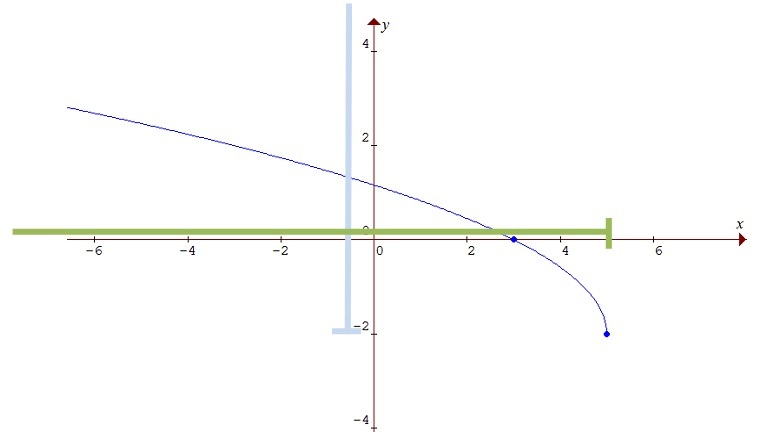
\includegraphics[height=5cm]{2_elem_rekenvaardigheden_B/inputs/reeel_vb1.jpg} 
%\end{figure}

%TODO figuur inladen 
\begin{figure}
	\centering          
	\input{2_elem_rekenvaardigheden_B/Fig_module_2_1_2_reele_functies_vb1}
	\caption{voorbeeld 1}
\label{fig:reele_functies_vb1}	
\end{figure}



\textbf{Domein}: de uitdrukking onder de vierkantswortel
mag niet negatief worden:


\begin{eqnarray*}
	\begin{array}{cccc}
		& 10-2x & \geqslant & 0\\
		\iff & 10 & \geqslant & 2x\\
		\iff & 5 & \geqslant & x\\
		\iff & x & \leqslant & 5
	\end{array}
\end{eqnarray*}


Besluit: voor $x$ zijn alle waarden van $-\infty$ tot
en met $5$ toegelaten. We schrijven: $\textrm{dom}\ f(x)=]-\infty,5]$ 

\textbf{Beeld}: de kleinste functiewaarde wordt
bekomen als de wortel $0$ is. Vierkantwortels geven altijd een positief
resultaat (of nul). De uitdrukking onder de wortel wordt $0$ als
$x=5$. We zien dat $f(5)=-2$. Er is geen bovengrens, dus het bereik
loopt tot $+\infty$.

Besluit: $\textrm{bld}f=[-2,+\infty[$




\textbf{Nulpunten}: voor welke waarden van $x$ wordt $f(x)=0$?


\begin{eqnarray*}
	\begin{array}{cccc}
		& \sqrt{10-2x}-2 & = & 0\\
		\iff & \sqrt{10-2x} & = & 2\\
		\iff & \left(\sqrt{10-2x}\right)^{2} & = & 2^{2}\\
		\iff & 10-2x & = & 4\\
		\iff & 6 & = & 2x\\
		\iff & x & = & 3
	\end{array}
\end{eqnarray*}


Besluit: er is slechts 1 nulwaarde, en dit is $x=3$ .




\textbf{Symmetrie}: we gaan na of het beeld van $-x$ hetzelfde
of het tegengestelde resultaat geeft als de gegeven functie. $f(-x)=\sqrt{10-2(-x)}-2=\sqrt{10+2x}-2$.
Dit is noch gelijk aan $f(x)$ noch gelijk aan $-f(x)$. Deze functie
is dus noch even, noch oneven.

\end{voorbeeld}

\begin{voorbeeld}
	Bespreek de functie met voorschrift $f(x)=\frac{1}{x-2}$.

%\begin{figure}[h]
%	\centering{}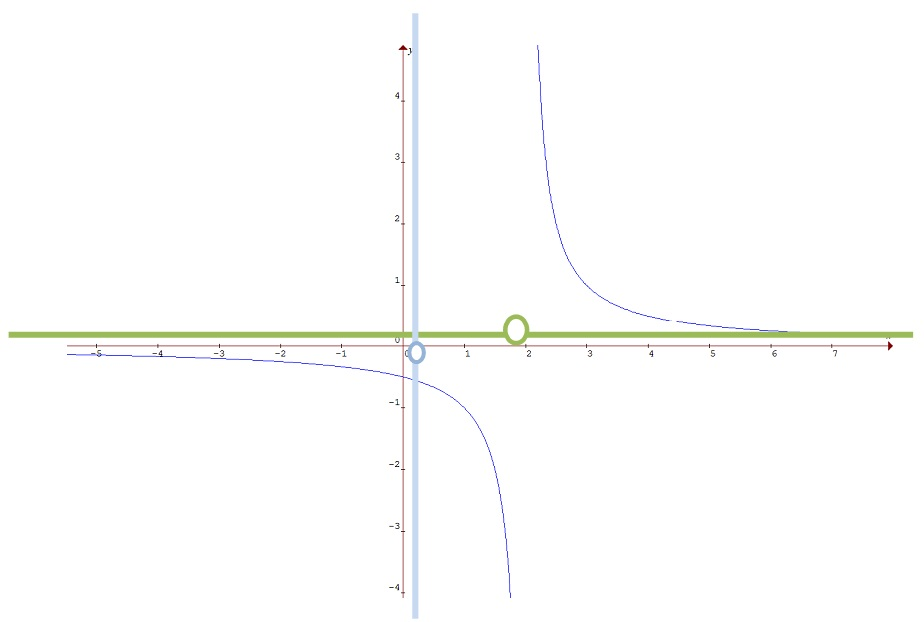
\includegraphics[height=5cm]{2_elem_rekenvaardigheden_B/inputs/reeel_vb2.jpg} 
%\end{figure}

%TODO figuur inladen

\begin{figure}
	\centering          
	\input{2_elem_rekenvaardigheden_B/Fig_module_2_1_2_reele_functies_vb2}
	\caption{voorbeeld 2}
	\label{fig:reele_functies_vb2}	
\end{figure}




\textbf{Domein}: de noemer mag niet nul worden (omdat een
getal delen door $0$ geen getal $\in \mathbb{R}$ is):


\begin{eqnarray*}
	\begin{array}{cccc}
		& x-2 & \neq & 0\\
		\iff & x & \neq & 2
	\end{array}
\end{eqnarray*}


Besluit: $\textrm{dom}\:y=\mathbb{R}\setminus\{2\}$ 




\textbf{Beeld}: er is geen bovengrens en geen ondergrens,
maar de breuk zal echter nooit $0$ worden.

Besluit: $\textrm{bld}f=\mathbb{R}_{0}$




\textbf{Nulpunten}: aangezien een breuk enkel nul kan worden
als de teller nul is, zal dit bij deze functie nooit gebeuren. Er
is dus geen snijpunt met de $x$-as.

Besluit: deze functie heeft geen nulpunten.




\textbf{Symmetrie}: we gaan na of het beeld van $-x$ hetzelfde
of het tegengestelde resultaat geeft als de gegeven functie. $f(-x)=\frac{1}{(-x)-2}=-\frac{1}{x+2}$.
Dit is noch gelijk aan $f(x)$ noch gelijk aan $-f(x)$. Deze functie
is dus noch even, noch oneven.

\end{voorbeeld}

\begin{voorbeeld}
	Bespreek de sinusfunctie $f(x)=\sin(x)$ 

%\begin{figure}[h]
%	\centering{}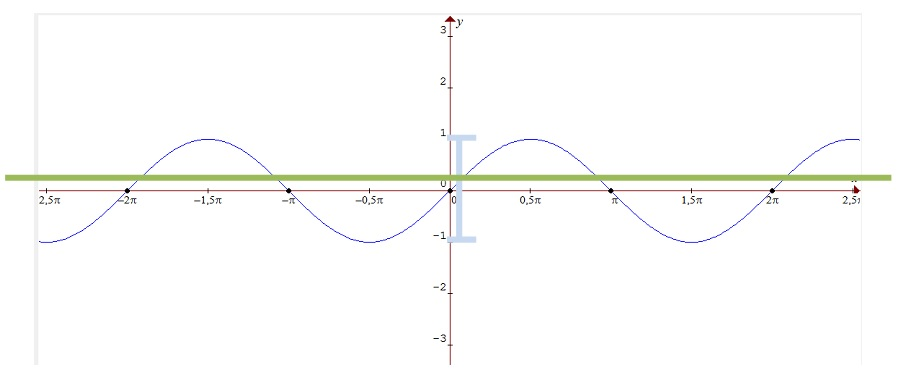
\includegraphics[height=5cm]{2_elem_rekenvaardigheden_B/inputs/reeel_vb3.jpg} 
%\end{figure}

%TODO figuur inladen
\begin{figure}
	\centering          
	\input{2_elem_rekenvaardigheden_B/Fig_module_2_1_2_reele_functies_vb3}
	\caption{voorbeeld 3}
	\label{fig:reele_functies_vb3}	
\end{figure}


\textbf{Domein}: we mogen op de plaats van $x$ gelijk welke
hoek invullen, de sinus zal steeds bestaan.

Besluit: $\textrm{dom}\:y=\mathbb{R}$ 




\textbf{Beeld}: we lezen op de $y$-as het beeld af. De
functiewaarden voor de sinus kunnen nooit groter zijn dan $1$ of
kleiner dan $-1$

Besluit: $\textrm{bld}f=[-1,1]$




\textbf{Nulpunten}: de $x$-as wordt gesneden als $\sin(x)=0$.
Dit gebeurt zowel voor $x$-waarden gelijk aan $\{0,\pi,2\pi,3\pi,...\}$
als ook voor $\{...,-3\pi,-2\pi,-\pi,0\}$

Besluit: de snijpunten met de $x$-as zijn de punten $\{...,(-2\pi,0),(-\pi,0),(0,0),(\pi,0),(2\pi,0),...\}$
of iets korter genoteerd als: $\{(k\pi,0)\:\textrm{met}\:k\in\mathbb{Z}\}$




\textbf{Symmetrie}: via de goniometrische formules vinden
we snel dat $f(-x)=\sin(-x)=-\sin(x)=-f(x)$ , dus kunnen we zeggen
dat deze functie oneven is (symmetrisch t.o.v. de oorsprong).

\end{voorbeeld}
%\subsection{Verloop van functies}

\subsubsection{Absolute en relatieve extrema}


\begin{definitie}
	Een functie $f$ heeft een \textbf{absoluut maximum} $f(x_{0})$
in het punt $x_{0}\in\textrm{dom}\:f$, als voor alle $x\in\textrm{dom}\:f$
geldt dat $f(x_{0})\geqslant f(x)$

Een functie $f$ heeft een \textbf{absoluut minimum} $f(x_{0})$
in het punt $x_{0}\in\textrm{dom}\:f$, als voor alle $x\in\textrm{dom}\:f$
geldt dat $f(x_{0})\leqslant f(x)$

Een functie $f$ heeft een \textbf{relatief of lokaal maximum}
in het punt $x_{0}$, indien er een open interval $I$ bestaat rond
het punt $x_{0}$ zodat voor alle $x$ in het interval $I$ geldt
dat $f(x_{0})\geqslant f(x)$

Een functie $f$ heeft een \textbf{relatief of lokaal minimum}
in het punt $x_{0}$, indien er een open interval $I$ bestaat rond
het punt $x_{0}$ zodat voor alle $x$ in het interval $I$ geldt
dat $f(x_{0})\leqslant f(x)$

\end{definitie}


\begin{voorbeeld}
%TODO figuur aanpassen  	

\begin{figure}[h]
	\centering          
	\input{2_elem_rekenvaardigheden_B/Fig_module_2_1_2_verloop_vb1}
	\caption{voorbeeld 1}
	\label{fig:verloop_vb1}	
\end{figure}


Voor de functie in gegeven in bovenstaande figuur zijn $x_{1},\:x_{2},\:x_{3},\:x_{4}$ relatieve of lokale extrema. Hiervan zijn $x_{2}$ en $x_{3}$ absolute extrema.

$x_{1},\:x_{3}$ zijn relatieve of lokale maxima.
Hiervan is $x_{3}$ een absoluut maximum.

$x_{2},\:x_{4}$ zijn relatieve of lokale minima. Hiervan
is $x_{2}$ een absoluut minimum.

\end{voorbeeld}

\subsubsection{Stijgen, dalen en extrema}

De eerste afgeleide speelt een belangrijke rol bij het onderzoek
naar het verloop van een functie. Men zal dus het tekenverloop van
deze afgeleide onderzoeken.




\begin{definitie}
	Als de eerste afgeleide $f^{'}(x)>0$ is in een interval,
dan zal deze functie in dat interval \textbf{stijgen}.

Als de eerste afgeleide $f^{'}(x)<0$ is in een interval,
dan zal deze functie in dat interval \textbf{dalen}.

De functie zal een relatief of lokaal extremum (maximum
of minimum) bereiken waar de kromme overgaat van een stijgende functie
naar een dalende functie of omgekeerd.

Een functie $f(x)$ heeft in het punt $(x_{0},y_{0})$ een
extremum als in dat punt aan de volgende voorwaarden voldaan is:

\begin{itemize}
\item als $f^{'}(x_{0})=0$ en $f^{''}(x_{0})>0$ zal het
extremum een minimum zijn, en
\item als $f^{'}(x_{0})=0$ en $f^{''}(x_{0})<0$ zal het
extremum een maximum zijn.
\end{itemize}

\end{definitie}

\begin{opmerking}
	\ \\
	\begin{itemize}
\item Opmerking 1: in een extremum bezit de functie een horizontale
raaklijn (aangezien $f^{'}(x_{0})=0$ is).
\item Opmerking 2: indien $f^{'}(x_{0})=0$ en ook $f^{''}(x_{0})=0$
werkt deze methode niet om na te gaan of er in $x_{0}$ een extremum
is. In dat geval gaan we naar de derde afgeleide kijken. Als $f^{'''}(x_{0})\neq0$
dan is het punt $x_{0}$ een buigpunt. Indien ook de derde afgeleide
nul is moeten we naar de eerstvolgende afgeleide gaan kijken die niet
nul is. Stel dat deze van de n$^{de}$ orde is, dus $f^{(n)}(x_{0})\neq0$
. Als dan $n$ even is, is er in $x_{0}$ een lokaal minimum als $f^{(n)}(x_{0})>0$
, en een lokaal maximum als $f^{(n)}(x_{0})<0$ . Is de n$^{de}$
oneven dan is $x_{0}$ terug een buigpunt. 

Tip: als je dit moeilijk
kan onthouden, denk dan aan de eenvoudige functies $f(x)=x^{2}$ en
$f(x)=x^{3}$ . De functie $x^{2}$ heeft een minimum in nul, terwijl
$x^{3}$ in de oorsprong een buigpunt heeft.
\end{itemize}

\end{opmerking}



\begin{voorbeeld}
	Onderzoek het stijgen en dalen van volgende functie $f$ met voorschrift: $f(x)=x^{3}-3x^{2}$ in onderstaande figuur.
	
	\gewonefiguur{width=.7\linewidth}{2_elem_rekenvaardigheden_B/inputs/verloop_vb2.jpg}

De eerste afgeleide $f^{'}(x)=3x^{2}-6x$ is nul als $3x^{2}-6x=3x(x-2)=0$, dus als $x=0$ of als $x=2$.

Om de $y$-co\"ordinaat van deze extrema punten te vinden
vullen we $x=0$ en $x=2$ in in de functie $f(x)$. Dit geeft: $f(0)=0$
en $f(2)=-4$.

De functie $f$ zal in de punten $(0,0)$ en $(2,-4)$ een
extremum bezitten. In het punt $(0,0)$ is dit een maximum en in het
punt $(2,-4)$ een minimum. De raaklijn is in die punten ook telkens
horizontaal.

Aangezien de eerste afgeleide een tweedegraadsfunctie is,
zullen we het tekenverloop van de tweedegraadsfunctie toepassen, zie onderstaande tabel.

%\begin{table}
%	\centering
\begin{center}
	\begin{tabular}{c||c|c|c|c|c}
	$x$ &  & 0 &  & 2 & \tabularnewline
	\hline 
	$f^{'}(x)=3x(x-2)$ & + & 0 & - & 0 & + \\
	\hline 
	$f(x)$ &  & 0 &  & -4 & \\
	& $\nearrow$ & max & $\searrow$ & min & $\nearrow$ \\
\end{tabular}
\end{center}

%\caption{Voorbeeld stijgen, dalen en extrema.}
%\label{tab:stijgen}
%\end{table}

%\begin{figure}[h]
%\centering{}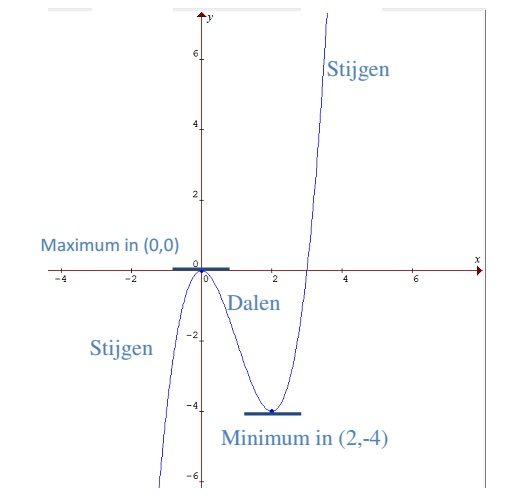
\includegraphics[width=.7\linewidth]{2_elem_rekenvaardigheden_B/inputs/verloop_vb2.jpg}
%\caption{Voorbeeld stijgen en dalen.}
%\label{fig:vb2}
%\end{figure}

\end{voorbeeld}

\subsubsection{Convex, concaaf en buigpunten}

Ook de tweede afgeleide speelt een belangrijke rol bij het
onderzoek naar het verloop van een functie. Men zal dus ook het tekenverloop
van de tweede afgeleide onderzoeken.


\begin{definitie}
	Als de tweede afgeleide $f^{''}(x)>0$ is in een interval,
dan zal de functie in dat interval \textbf{hol of concaaf} zijn (symbool:
$\bigcup$).

Als de tweede afgeleide $f^{''}(x)<0$ is in een interval,
dan zal de functie in dat interval \textbf{bol of convex} zijn (symbool:
$\bigcap$).

Punten waar de kromme overgaat van convex naar concaaf of
omgekeerd, noemt men \textbf{buigpunten}. In een buigpunt verandert
dus de tweede afgeleide van teken. Een functie $f(x)$ heeft in het
punt $(x_{0},y_{0})$ een buigpunt als in dat punt aan de volgende
voorwaarden voldaan zijn: $f^{''}(x_{0})=0$ en $f^{'''}(x_{0})\neq0$

\end{definitie}


\begin{opmerking}
	\ \\
	\begin{itemize}
	\item Opmerking 1: in een buigpunt snijdt de raaklijn de kromme,
	deze raaklijn noemt men de buigraaklijn.
	
	\item Opmerking 2: aangezien de kromming in een buigpunt verandert,
	is een buigpunt nooit een extremum.
\end{itemize}

\end{opmerking}


\begin{voorbeeld}
	Onderzoek het hol en bol zijn van
de functie $f$ met voorschrift $f(x)=x^{3}-3x^{2}$, zie onderstaande figuur.

\gewonefiguur{width=.7\linewidth}{2_elem_rekenvaardigheden_B/inputs/verloop_vb3.jpg}

De eerste afgeleide is $f^{'}(x)=3x^{2}-6x$ 

De tweede afgeleide is $f^{''}(x)=6x-6$ en is nul als $6x-6=6(x-1)=0$
, en dus als $x=1$.

Om de $y$-co\"ordinaat van dit buigpunt te vinden vullen
we $x=1$ in in de functie $f(x)$. Dit geeft: $f(1)=-2$.

Aangezien de tweede afgeleide een eerstegraadsfunctie is,
zullen we het tekenverloop van de eerstegraadsfunctie toepassen, zie onderstaande tabel.

%\begin{table}
%	\centering
\begin{center}
	\begin{tabular}{c||c|c|c}
	$x$ &  & 1 & \tabularnewline
	\hline 
	$f^{''}(x)=6(x-1)$ & - & 0 & +\\
	\hline 
	$f(x)$ & $\bigcap$ & -2 & $\bigcup$\\
	&  & buigpunt & \\
\end{tabular}
\end{center}
%\caption{Voorbeeld convex, concaaf en buigpunten}
%\label{tab:convex}
%\end{table}

\end{voorbeeld}
\begin{voorbeeld}
	Wat kan je zeggen over de functie $f$ met voorschrift
$f(x)=x^{3}$ in het punt waar $x=0$ is?

De eerste afgeleide is $f^{'}(x)=3x^{2}$ en is nul als
$x=0$. Dus $x=0$ kan een extremum zijn.

De tweede afgeleide is $f^{''}(x)=6x$ en is nul als $x=0$.
We kunnen niks zeggen; we moeten naar de eerstvolgende afgeleide gaan
kijken die niet nul is.

De derde afgeleide is $f^{'''}(x)=6$. De derde orde afgeleide
(n=3 is oneven) is niet nul, dus het punt $x=0$ is een buigpunt (en
geen extremum).

\end{voorbeeld}

\begin{voorbeeld}
	Zoek de buigpunten van de functie $f$ met voorschrift
$f(x)=\cos(x)$.

De eerste afgeleide is $f^{'}(x)=-\sin(x)$. De nulpunten
van $\sin x$ zijn $\{x=n\pi\:\textrm{met}\:n\in\mathbb{Z}\}$. In
deze punten kan $f(x)=\cos(x)$ een extremum bereiken.

De tweede afgeleide is $f^{''}(x)=-\cos(x)$. De nulpunten
van $\cos(x)$ zijn $\{x=\frac{\pi}{2}+n\pi\:\textrm{met}\:n\in\mathbb{Z}\}$.
In deze punten verandert de cosinus en dus ook de tweede afgeleide
van teken, dus dit zijn buigpunten. M.a.w. de nulpunten van de functie
$f(x)=\cos(x)$ zijn tevens de buigpunten (dit geldt ook voor de sinus).

\end{voorbeeld}
\subsection{Eerste- en tweedegraadsfuncties}
\label{sec:eerste_tweede}

\subsubsection{Constante functies}

\begin{definitie}
	Functievoorschrift: $f(x)=a$ met $a\in\mathbb{R}$
\end{definitie}

%\uline{Voorbeeld}: $f(x)=2$

\textbf{Grafische voorstelling van de constante functie}
met vergelijking $f(x)=a$ is een horizontale rechte, waarbij de $y$-as
wordt gesneden in het punt $(0,a)$.

%Alle afgeleiden zijn overal nul, er zijn geen extrema, geen
%buigpunten...

Tekenverloop: 

\begin{tabel}{Tekenverloop van een constante functie}
	\begin{tabular}{c||c}
		$x$ & \\
		\hline 
		$f(x)$ & teken van $a$\\
	\end{tabular}
	\label{tab:ct}
\end{tabel}


\begin{voorbeeld}
	Gegeven de functie: $f(x)=\frac{1}{2}$. 
%TODO figuur

\begin{figure}[h]
	\centering          
	\input{2_elem_rekenvaardigheden_B/Fig_module_2_1_4_constante_functie}
	\caption{Voorbeeld constante functie}
	\label{fig:constante_functie}	
\end{figure}
	
 
Grafische voorstelling:
\begin{itemize}
\item het domein van de constante functie is altijd: $\textrm{dom}f=\mathbb{R}$
\item het beeld van deze constante functie is: $\textrm{bld}f=\frac{1}{2}$
\end{itemize}
%\begin{figure}[h]
%\centering{}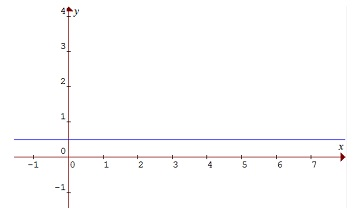
\includegraphics[height=5cm]{2_elem_rekenvaardigheden_B/inputs/constantefuncties.jpg} 
%\caption{Voorbeeld constante functie.}
%\label{fig:ct}
%\end{figure}

Tekenverloop

\begin{center}
\begin{tabular}{c||c}
	$x$ & \\
	\hline 
	$f(x)$ & $+$ \\
\end{tabular}	
\end{center}

\end{voorbeeld}

\subsubsection{Eerstegraadsfuncties of lineaire functies}

\begin{definitie}
	Functievoorschrift: $f(x)=ax+b$ met $a\in\mathbb{R}_{0}$
en $b\in\mathbb{R}$.

\end{definitie}


\begin{voorbeeld}
	 $f(x)=10x+1$ , $f(x)=8-5x$ , $f(x)=3x$
\end{voorbeeld}

Grafische voorstelling van de lineaire functie is een rechte.

%TODO figuur

\begin{figure}[h]
	\centering          
	\input{2_elem_rekenvaardigheden_B/Fig_module_2_1_4_eerstegraadsfunctie_1}
	\caption{Voorbeeld van een eerstegraadsfunctie}
	\label{fig:eerstegraadsfunctie}	
\end{figure}



%\gewonefiguur{height=5cm}{2_elem_rekenvaardigheden_B/inputs/eerstegraadsfuncties1.jpg}

\begin{itemize}
	\item Het domein van elke lineaire functie is: $\textrm{dom} f = \mathbb{R}$.
	\item Het beeld van deze lineaire functie is: $\textrm{bld} f = \mathbb{R}$.
\end{itemize}

De rechte wordt bepaald door de \textbf{richtingsco\"effici\"ent}
(de \textbf{rico}) \textquoteleft $a$\textquoteright{} en de intercept
\textquoteleft $b$\textquoteright . De rico bepaalt de helling van
de rechte. Als $x$ met 1 eenheid toeneemt, dan neemt $y$ met $a$
eenheden toe. Hoe groter de absolute waarde van de rico $a$, hoe
steiler de rechte.
\begin{itemize}
\item een positieve rico hoort bij een stijgende rechte
\item een negatieve rico hoort bij een dalende rechte
\end{itemize}


%TODO figuur

%M\begin{tabular}{ccc}
	%\hline
%	\input{2_elem_rekenvaardigheden_B/Fig_module_2_1_4_teken_rico_pos}	&\input{2_elem_rekenvaardigheden_B/Fig_module_2_1_4_rico_nul} &  \input{2_elem_rekenvaardigheden_B/Fig_module_2_1_4_teken_rico_neg}  \\
	%\hline
%\end{tabular}


\begin{figure}[h]
	\centering
	\begin{subfigure}{0.3\textwidth}
	\input{2_elem_rekenvaardigheden_B/Fig_module_2_1_4_teken_rico_pos}
	\caption{}
	\label{fig:rico_pos}	
	\end{subfigure}
	\begin{subfigure}{0.3\textwidth}
	\input{2_elem_rekenvaardigheden_B/Fig_module_2_1_4_rico_nul}
	\caption{}
	\label{fig:rico_nul}	
	\end{subfigure}
	\begin{subfigure}{0.3\textwidth}
	\input{2_elem_rekenvaardigheden_B/Fig_module_2_1_4_teken_rico_neg}
	\caption{}
	\label{fig:rico_neg}	
\end{subfigure}
\caption{Het teken van de richtingscoëfficiënt bepaalt of de rechte stijgt, constant is of daalt.}
\label{fig:rico}

\end{figure}
  


%\gewonefiguur{width=\linewidth}{2_elem_rekenvaardigheden_B/inputs/eerstegraadsfuncties2.jpg}

Een rechte evenwijdig met de $x$-as heeft een rico gelijk
aan 0. Dit is in feite de constante functie $f(x)=b$.

Een rechte evenwijdig met de $y$-as heeft geen rico (in
dit geval zou $m=\infty$ moeten zijn). 

Nulpunten: het snijpunt met de $x$-as is het
punt $(-\frac{b}{a},0)$.

%\uline{De eerste afgeleide} van $f(x)$ is $f^{'}(x)=(mx+b)^{'}=m$.
%Dit betekent dat de eerste afgeleide ons meteen vertelt of het om
%een stijgende of een dalende rechte gaat.
%
%Er zijn geen extrema, geen buigpunten...

Tekenverloop: 
\begin{tabel}{Tekenverloop voor $a>0$}
	\centering\begin{tabular}{c||c|c|c}
		$x$ &  & $-\frac{b}{a}$ & \\
		\hline 
		$f(x)$ & - & 0 & +\\
	\end{tabular}
\end{tabel}

\begin{tabel}{Tekenverloop voor $a<0$.}
	\centering\begin{tabular}{c||c|c|c}
		$x$ &  & $-\frac{b}{a}$ & \\
		\hline 
		$f(x)$ & + & 0 & -\\
	\end{tabular}
	\label{tab:eerst_akl0}
\end{tabel}

\begin{voorbeeld}
	Gegeven de functie: $f(x)=-2x+3$.
	

Grafische voorstelling:
\begin{itemize}
\item het domein van elke lineaire functie is: $\textrm{dom}f=\mathbb{R}$
\item het beeld van deze lineaire functie is: $\textrm{bld}f=\mathbb{R}$
\end{itemize}
%TODO figuur vervangen 


\begin{figure}[h]
	\centering          
	\input{2_elem_rekenvaardigheden_B/Fig_module_2_1_4_eerstegraadsfunctie_3}
	\caption{Voorbeeld van de grafische voorstelling van een eerstegraadsfunctie}
	\label{fig:eerstegraadsfunctie_3}	
\end{figure}

%\gewonefiguur{height=5cm}{2_elem_rekenvaardigheden_B/inputs/eerstegraadsfuncties3.jpg}

%\begin{figure}[h]
%\centering{}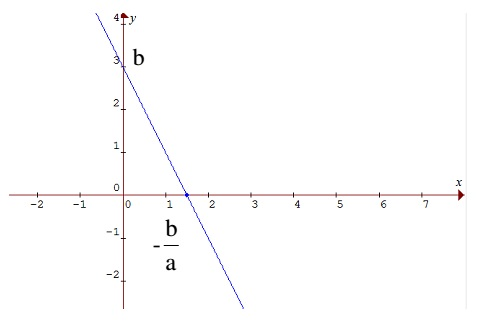
\includegraphics[height=5cm]{2_elem_rekenvaardigheden_B/inputs/eerstegraadsfuncties3.jpg}
%\caption{Voorbeeld grafische voorstelling van de eerstegraadfunctie.}
%\label{fig:eerste_vb_graf} 
%\end{figure}

Nulpunten:

We lossen de vergelijking $y=f(x)=-2x+3=0$ op en vinden:
$x=\frac{3}{2}$. Het snijpunt met de $x$-as is het punt $(\frac{3}{2},0)$.

Tekenverloop: zie Tabel \ref{tab:eerste_vb}.

\begin{tabel}{Voorbeeld eerstegraadsfunctie: tekenverloop}
\begin{tabular}{c||c|c|c}
	$x$ &  & $\frac{3}{2}$ & \\
	\hline 
	$f(x)$ & $+$ & 0 & $-$\\
\end{tabular}
\label{tab:eerste_vb}	
\end{tabel}

\end{voorbeeld}

\subsubsection{Tweedegraadsfuncties of kwadratische functies}



\begin{definitie}
	Functievoorschrift: $f(x)=ax^{2}+bx+c$ met $a\in\mathbb{R}_{0}$
en $b,c\in\mathbb{R}$ 

\end{definitie}

\begin{voorbeeld}
	$f(x)=3x^{2}+10x+1$ , $f(x)=-2x^{2}+5$
, $f(x)=x^{2}$
\end{voorbeeld}

Grafische voorstelling van de kwadratische functie
is een parabool.
%TODO figuur  vervangen 
\gewonefiguur{width=.7\linewidth}{2_elem_rekenvaardigheden_B/inputs/tweedegraadsfuncties1.jpg}

%\begin{figure}[h]
%\centering{}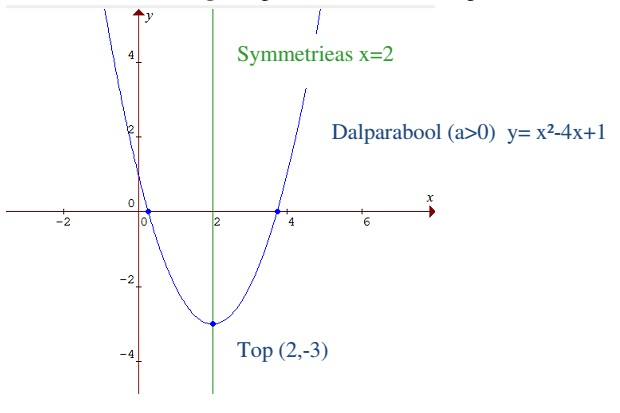
\includegraphics[width=.7\linewidth]{2_elem_rekenvaardigheden_B/inputs/tweedegraadsfuncties1.jpg}
%\caption{Grafische voorstelling van een tweedegraadsfunctie.}
%\label{fig:tweede} 
%\end{figure}

\begin{itemize}
\item als $a>0$ is de top van de \textbf{dalparabool} het minimum
\item als $a<0$ is de top van de \textbf{bergparabool} het maximum
\end{itemize}
Hoe groter de absolute waarde van $a$, hoe smaller de opening
van de parabool is.

De verticale lijn door de top is de \textbf{symmetrieas}.
De vergelijking van de symmetrieas is: $x=-\frac{b}{2a}$ 

Het laagste punt van een dalparabool of het hoogste punt
van een bergparabool heet de \textbf{top} van de parabool. De top
is het snijpunt van de parabool met de verticale symmetrieas. De co\"ordinaten
van de top zijn dus $(-\frac{b}{2a},y)$. De $y$-waarde vinden we
door de gevonden $x$-waarde in het functievoorschrift $f(x)$ in
te vullen, dus $y=f(-\frac{b}{2a})$ .

Nulpunten: stellen we $y=f(x)=ax^{2}+bx+c=0$
(in dat geval spreken we van de \textbf{vierkantsvergelijking}), dan
vinden we de snijpunten met de $x$-as. Hiervoor moeten we dus de
(vierkants)vergelijking $ax^{2}+bx+c=0$ oplossen. Daarvoor bepaal
je best eerst de \textbf{discriminant} $D=b^{2}-4ac$ (van de abc
formule). Met de discriminant bepaal je het aantal snijpunten van
de kwadratische functie met de $x$-as.
\begin{itemize}
\item als $D>0$ , dan heeft de vergelijking twee oplossing: $x_{1}=\frac{-b+\sqrt{D}}{2a}$
en $x_{2}=\frac{-b-\sqrt{D}}{2a}$. De parabool snijdt de $x$-as
op twee plaatsen.
\item als $D=0$ , dan heeft de vergelijking \'e\'en oplossing: $x_{1}=x_{2}=-\frac{b}{2a}$.
De parabool raakt met zijn top de $x$-as in \'e\'en punt.
\item als $D<0$ , dan heeft de vergelijking geen re\"ele oplossingen. De
parabool ligt ofwel boven ofwel onder de $x$-as.
\end{itemize}

%TODO figuur vervangen 
\gewonefiguur{scale=0.8}{2_elem_rekenvaardigheden_B/inputs/tweedegraadsfuncties2.jpg}

%\begin{figure}[h]
%\centering{}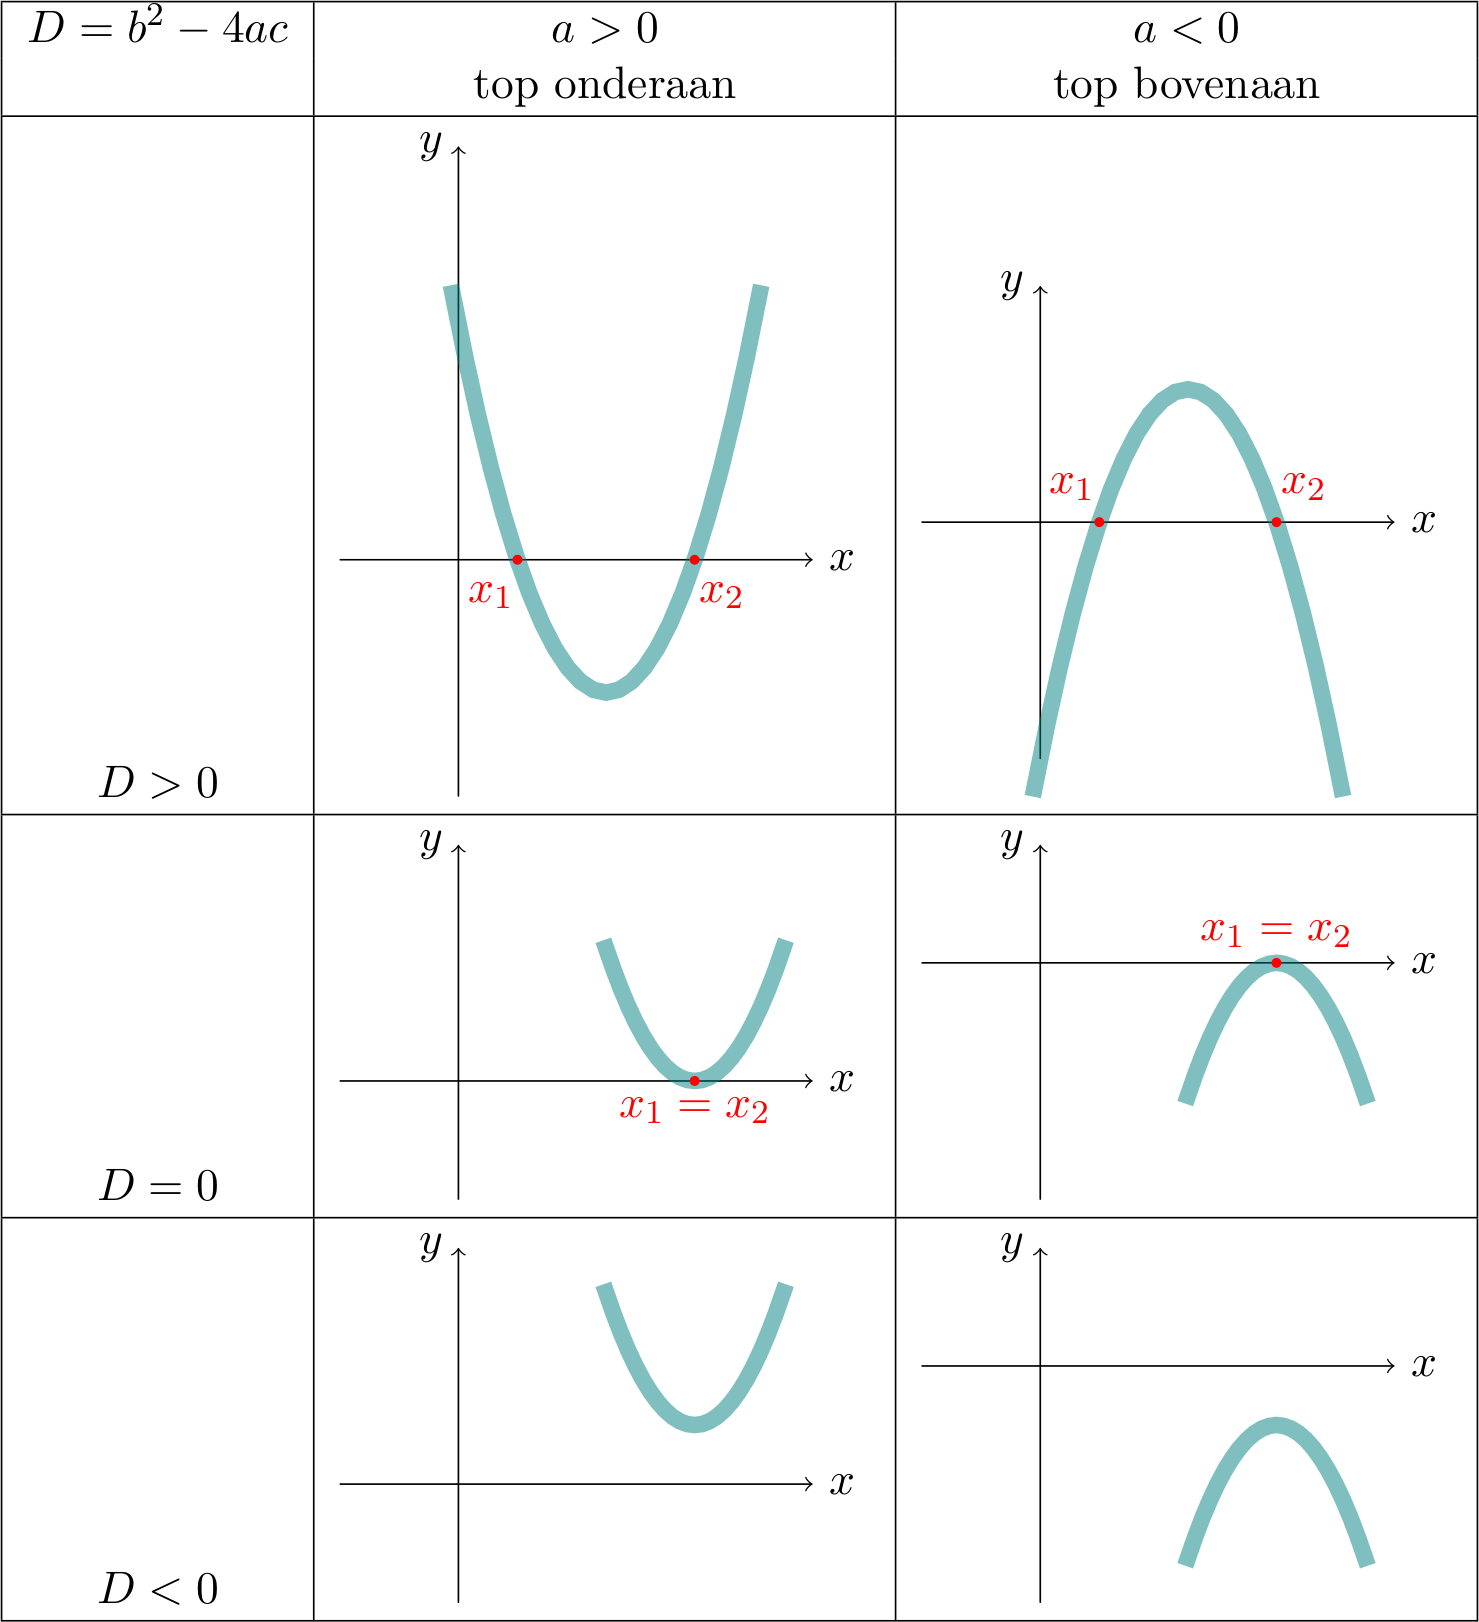
\includegraphics[scale=0.8]{2_elem_rekenvaardigheden_B/inputs/tweedegraadsfuncties2.jpg} 
%\caption{Grafische voorstelling van tweedegraadsfuncties voor verschillende waarden van $a$ en $D$.}
%\label{fig:tweede:gevallen}
%\end{figure}


%\uline{Opmerking}: stellen we de eerste afgeleide gelijk
%aan nul, dan vinden we de $x$-co\"ordinaat van de top: $f^{'}(x)=(ax^{2}+bx+c)^{'}=2ax+b=0$
%of $x=-\frac{b}{2a}$ . Het teken van de eerste afgeleide zegt ons
%of de functie (links en rechts van de top) stijgt of daalt. Tenslotte,
%het teken van de tweede afgeleide $f^{''}(x)=(2ax+b)^{'}=2a$, m.a.w.
%het teken van $a$ , zegt ons of het om een dal- of bergparabool gaat.

Tekenverloop:

\begin{itemize}
\item Als $D>0$ \\
\begin{center}
	\begin{tabular}{c||c|c|c|c|c}
$x$ &  & $x_{1}$ &  & $x_{2}$ & \\
\hline 
$f(x)$ & teken van $a$ & 0 & tegengesteld teken van $a$ & 0 & teken van $a$\\
\end{tabular}
\end{center}
\item Als $D=0$ \\
\begin{center}
	\begin{tabular}{c||c|c|c}
	$x$ &  & $x_{1}=x_{2}$ & \\
	\hline 
	$f(x)$ & teken van $a$ & 0 & teken van $a$\\
\end{tabular}
\end{center}
\item Als $D<0$ \\
\begin{center}
	\begin{tabular}{c||c}
$x$ & \\
\hline 
$f(x)$ & teken van $a$\\
\end{tabular}
\end{center}
\end{itemize}
%\begin{table}[h]
%\centering
%\caption{Algemeen tekenverloop van een tweedegraadsfunctie voor $D>0$}
%\end{table}
%\begin{tabular}{c|c}
%$D=0$ & %
%\begin{tabular}{c||c|c|c}
%$x$ &  & $x_{1}=x_{2}$ & \\
%\hline 
%\hline 
%$f(x)$ & teken van $a$ & 0 & teken van $a$\\
%\end{tabular}\\
% & \\
%\hline 
% & \\
%$D>0$ & %
%\begin{tabular}{c||c|c|c|c|c}
%$x$ &  & $x_{1}$ &  & $x_{2}$ & \\
%\hline 
%\hline 
%$f(x)$ & teken van $a$ & 0 & tegengesteld teken van $a$ & 0 & teken van $a$\\
%\end{tabular}\\
% & \\
%\hline 
% & \\
%$D<0$ & %
%\begin{tabular}{c||c}
%$x$ & \\
%\hline 
%\hline 
%$f(x)$ & teken van $a$\\
%\end{tabular}\\
%\end{tabular}


\begin{voorbeeld}
	Gegeven de functie $f$ met voorschrift: $f(x)=-x^{2}-5x+6$ 

Grafische voorstelling:
\begin{itemize}
\item het domein van elke kwadratische functie is: $\textrm{dom}f=\mathbb{R}$
\item $a=-1<0$ dus het is een bergparabool
\item de symmetrieas ligt bij $x=-\frac{b}{2a}=-\frac{-5}{2.(-1)}=-\frac{5}{2}=-2,5$
\item de top heeft de co\"ordinaten $(x,y)=(-\frac{b}{2a},f(-\frac{b}{2a}))=(-2,5;12,25)$
\item de top van deze bergparabool ligt op $y=12,25$. Dit is dus de grootste
waarde die $y$ kan bereiken. Het beeld van deze kwadratische functie
is daarom: $\textrm{bld}f=]-\infty;12,25]$
\end{itemize}


Nulpunten:

We lossen de vergelijking $y=f(x)=-x^{2}-5x+6=0$ op d.m.v.
de abc formule. We berekenen daarvoor eerst de discriminant $D$:

\begin{equation*}
D=b^{2}-4ac=(-5)^{2}-4.(-1).6=25+24=49
\end{equation*}

Omdat $D>0$ zijn er 2 re\"ele oplossingen, dus 2 snijpunten
met de $x$-as. Deze zijn:
\begin{itemize}
\item $x_{1}=\frac{-b+\sqrt{D}}{2a}=\frac{-(-5)+\sqrt{49}}{2.(-1)}=-6$
\item $x_{2}=\frac{-b-\sqrt{D}}{2a}=\frac{-(-5)-\sqrt{49}}{2.(-1)}=1$
\end{itemize}
De parabool snijdt de horizontale as in de koppels (-6,0) en (1,0)
en de top ligt boven de $x$-as (want het is een bergparabool).
%TODO figuur vervangen
\gewonefiguur{width=.5\linewidth}{2_elem_rekenvaardigheden_B/inputs/tweedegraadsfuncties3.jpg}

%\begin{figure}[h]
%\centering{}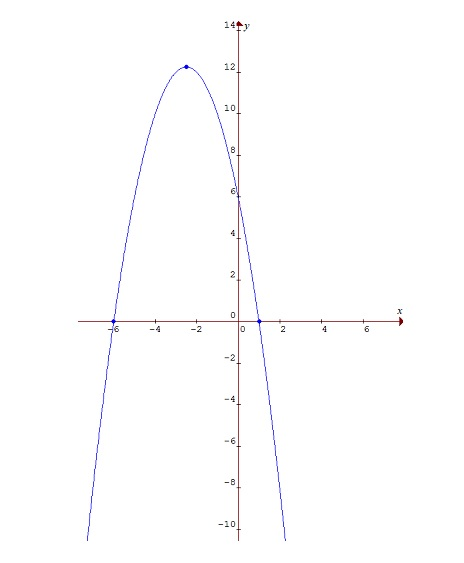
\includegraphics[width=.5\linewidth]{2_elem_rekenvaardigheden_B/inputs/tweedegraadsfuncties3.jpg}
%\caption{Voorbeeld tweedegraadsfuncties: grafische voorstelling}
%\label{fig:tweede:vb} 
%\end{figure}


Tekenverloop:


\begin{tabel}{Voorbeeld tweedegraadsfuncties: tekenverloop}
\begin{tabular}{c||c|c|c|c|c}
	$x$ &  & $-6$ &  & $1$ & \\
	\hline 
	$f(x)$ & $-$ & 0 & $+$ & 0 & $-$\\
\end{tabular}
\label{tab:tweede:vb}	
\end{tabel}

\end{voorbeeld}
\subsection{Tweedegraadsvergelijking - voorbeeld 1}
\begin{minipage}{.25\linewidth}
	\raggedright
	
\includegraphics[width=4cm]{2_elem_rekenvaardigheden_B/inputs/QR_Code_TWEEDEGRVGL1_module2new}
\end{minipage}
\begin{minipage}{.7\linewidth}
	Zie filmpje MOOC.
\end{minipage}
\subsection{Tweedegraadsvergelijking - voorbeeld 2}
\begin{minipage}{.25\linewidth}
	\raggedright
	
\includegraphics[width=4cm]{2_elem_rekenvaardigheden_B/inputs/QR_Code_TWEEDEGRVGL2_module2new}
\end{minipage}
\begin{minipage}{.7\linewidth}
	Zie filmpje MOOC.
\end{minipage}
%\input{2_elem_rekenvaardigheden_B/module_2_1_5}
%\input{2_elem_rekenvaardigheden_B/module_2_1_6}
%\subsection{Veeltermfuncties}

\subsubsection{Veeltermfuncties of polynoomfuncties}

\emph{Definitie}

Een veelterm- of polynoomfunctie heeft als functievoorschrift een veelterm in 1 onbekende, dus
$f(x)=a_{n}x^{n}+a_{n-1}x^{n-1}+\ldots+a_{2}x^{2}+a_{1}x+a_{0}$
met $a_{n}\in\mathbb{R}_{0}$ en $a_{n-1},\ldots,a_{0}\in\mathbb{R}$. De constanten $a_{i}$ noemen we de \textbf{co\"effici\"enten}.

De (meestal eerste) term met de hoogste macht bepaalt de \textbf{graad} van de veeltermfunctie.

\emph{Voorbeelden}

$f(x)=2x^{4}-5x^{3}+10x$ , $f(x)=x^{3}$ 

\textbf{Grafische voorstelling}

\noindent Het domein van een veeltermfunctie is: $\textrm{dom}f=\mathbb{R}$

\noindent De grafieken van de elementaire machtsfuncties $y=x^{n}$
met positieve exponent zijn hieronder weergegeven:

\begin{figure}[h]
\centering{}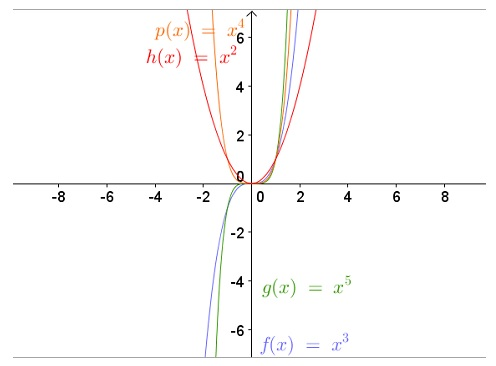
\includegraphics[height=5cm]{2_elem_rekenvaardigheden_B/inputs/veeltermfuncties1.jpg} 
\end{figure}


\noindent De grafieken van de elementaire machtsfuncties $y=x^{-n}=\frac{1}{x^{n}}$
met negatieve exponent zijn hieronder weergegeven:

\begin{figure}[h]
\centering{}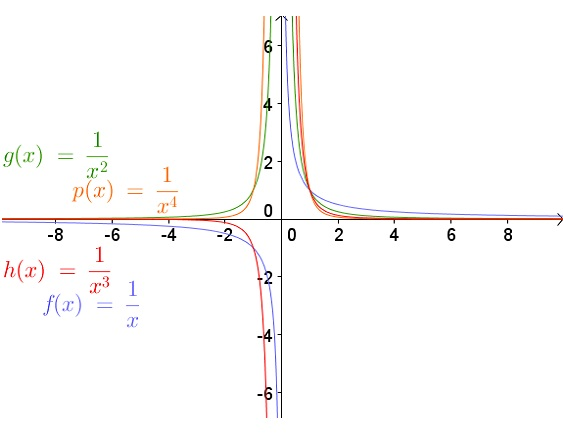
\includegraphics[height=5cm]{2_elem_rekenvaardigheden_B/inputs/veeltermfuncties2.jpg} 
\end{figure}


\textbf{Nulwaarden}

\noindent Een $n$\textsuperscript{de} graadsveeltermfunctie met oneven
$n$ heeft minimum $1$ en maximum $n$ snijpunten met de $x$-as.

\noindent Een $n$\textsuperscript{de} graadsveeltermfunctie met even
$n$ heeft minimum $0$ en maximum $n$ snijpunten met de $x$-as. De grafiek
kan namelijk helemaal boven of onder de $x$-as liggen, en dus geen
snijpunten hebben met de $x$-as.

\emph{Voorbeeld}

De functie $f$ met voorschrift $f(x)=2x^{4}-3x^{3}-x^{2}+x$ uit Figuur \ref{fig:vt:vb1}
is een 4\textsuperscript{de} graadsvergelijking en heeft in dit geval
4 snijpunten met de $x$-as:

\begin{figure}[h]
\centering{}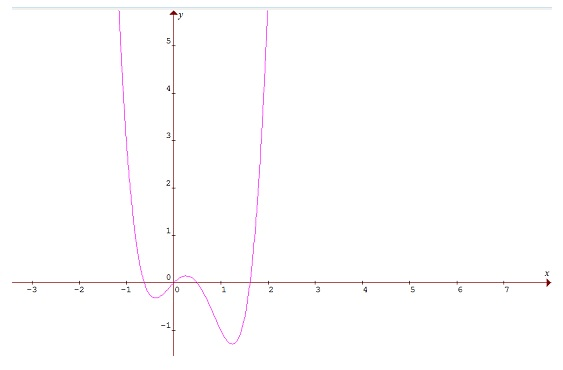
\includegraphics[height=5cm]{2_elem_rekenvaardigheden_B/inputs/veeltermfuncties3.jpg} 
\caption{Voorbeeld veeltermfunctie.}
\label{fig:vt:vb1}
\end{figure}

\textbf{Nulwaarden vinden}

De nulwaarden voor een veeltermfunctie vinden we door het
functievoorschrift te ontbinden in een product van factoren met ten
hoogste een tweede graad, m.a.w. we ontbinden de veeltermfunctie $f(x)$
in lineaire factoren $x+a$ en in kwadratische factoren $ax^{2}+bx+c$.
De nulpunten van de functie $f(x)$ zijn dan de nulpunten van de verschillende
factoren.

\textbf{Tekenverloop}

Eens een veelterm ontbonden is in factoren, is het eenvoudig
om het tekenverloop er van te bepalen. Het tekenverloop van een constante,
een lineaire en een kwadratische functie is immers gekend. Het teken
van een veeltermfunctie is het product van de tekens van de factoren.


\emph{Voorbeeld (een tweedegraadsfunctie verleiden door substitutie)}

Deze methode is toepasbaar bij bikwadratische vergelijkingen. Dit
zijn vergelijkingen van de vorm $ax^{4}+bx^{2}+c=0$. Dit type van
vergelijkingen kan herleid worden tot een kwadratische vergelijking
met behulp van de substitutiemethode. Stel hierbij $x^{2}=t$.

We bekijken de veelterm $f(x)=4x^{4}-5x^{2}+1$

\textbf{Nulwaarden}

\noindent We bepalen de nulwaarden door de veelterm te ontbinden in
factoren, gebruik makend van de substitutiemethode:\\

\begin{equation*}
4x^{4}-5x^{2}+1=0  \underrightarrow{x^{2}=t}  4t^{2}-5t+1=0
\end{equation*}

\noindent We bekomen een kwadratische vergelijking. Hiervan zijn de
nulpunten:
\begin{eqnarray*}
t_{1}=\frac{-b+\sqrt{D}}{2a}&=&\frac{-(-5)+\sqrt{9}}{2.4}=1 \\
t_{2}=\frac{-b-\sqrt{D}}{2a}&=&\frac{-(-5)-\sqrt{9}}{2.4}=\frac{1}{4}
\end{eqnarray*}

De 2 oplossingen voor $t$ zijn $t_{1}=1$ en $t_{2}=\frac{1}{4}$
zodat de vergelijking kan geschreven worden als: $4t^{2}-5t+1=(t-1)(t-\frac{1}{4})$.

Aangezien $x^{2}=t$ zijn de 4 oplossingen voor $x$: $x_{1en2}=\pm\sqrt{t_{1}}$
en $x_{3en4}=\pm\sqrt{t_{2}}$ 

Dit geeft $x_{1}=1$ , $x_{2}=-1$ , $x_{3}=\frac{1}{2}$
en $x_{4}=-\frac{1}{2}$.

De gegeven vergelijking kan dus ook geschreven worden als:

\begin{equation*}
f(x)=4x^{4}-5x^{2}+1=(x-1)(x+1)(x-\frac{1}{2})(x+\frac{1}{2})
\end{equation*}

\textbf{Tekenverloop}

Maak \'e\'en overzichtelijke tabel met bovenaan alle nulpunten
in stijgende volgorde. Per rij onderzoek je het teken van elke factor
van $f(x)$. Het teken van $f(x)$ is dan het product van deze tekens.

\begin{center}
\begin{tabular}{c||ccccccccc}
$x$ &  & $-1$ &  & $-\frac{1}{2}$ &  & $\frac{1}{2}$ &  & $1$ & \\
\hline 
$(x-1)$ & - & - & - & - & - & - & - & $0$ & $+$\\
$(x-\frac{1}{2})$ & - & - & - & - & -  & $0$ & + & + & + \\
$(x+\frac{1}{2})$ & - & - & - & $0$ & + & + & + & + & + \\
$(x+1)$ & $-$ & $0$ & + & + & + & + & + & + & + \\
\hline 
$f(x)$ & $+$ & $0$ & $-$ & $0$ & $+$ & $0$ & $-$ & $0$ & $+$\\
\end{tabular}
\end{center}


\emph{Voorbeeld 2 (ontbinden in factoren)}

We bekijken de veelterm $f(x)=3x^{3}-4x^{2}-6x+8$

\textbf{Nulpunten}

We bepalen de nulpunten door de veelterm te ontbinden in
factoren. Soms kunnen we gebruik maken van merkwaardige producten
of, zoals in dit geval, door het groeperen van gemeenschappelijke
termen:

\begin{eqnarray*}
3x^{3}-4x^{2}-6x+8 & = & (3x^{3}-4x^{2})-(6x-8)\\
 & = & x^{2}(3x-4)-2(3x-4)\\
 & = & (x^{2}-2)(3x-4)\\
 & = & (x-\sqrt{2})(x+\sqrt{2})(3x-4)
\end{eqnarray*}

\noindent De gegeven vergelijking $3x^{3}-4x^{2}-6x+8=0$ heeft dus
3 nulpunten:

\begin{equation*}
x_{1}=\sqrt{2}, x_{2}=-\sqrt{2} \text{ en } x_{3}=\frac{4}{3}
\end{equation*}

\textbf{Tekenverloop}

Maak \'e\'en overzichtelijke tabel met bovenaan alle nulpunten
in stijgende volgorde. Per rij onderzoek je het teken van elke factor
van $f(x)$. Het teken van $f(x)$ is dan het product van deze tekens.

\begin{center}
\begin{tabular}{c||ccccccc}
$x$ &  & $-\sqrt{2}$ &  & $\frac{4}{3}$ &  & $\sqrt{2}$ & \\
\hline 
$(x-\sqrt{2})$ & - & - & -& -& - & $0$ & $+$ \\
$(x+\sqrt{2})$ & $-$ & $0$ & + & + & +&+&+ \\
$(3x-4)$ & - & - & - & $0$ & +&+&+ \\
\hline 
$f(x)$ & $-$ & $0$ & $+$ & $0$ & $-$ & $0$ & + \\
\end{tabular}
\end{center}


\emph{Voorbeeld 3 (regel van Horner)}

We bekijken de veelterm $f(x)=x^{4}-4x^{3}+5x^{2}-4x+4$

\textbf{Nulpunten}

We bepalen de nulpunten door de veelterm te ontbinden in
factoren gebruik makend van de regel van Horner.

Ga na welke mogelijke delers van $a_{0}$ kunnen afgesplitst
worden zonder rest. Hier zijn de delers van $a_{0}=4$: $\pm1,\:\pm2\:\textrm{en}\:\pm4$

We proberen $x=+2$: $f(2)=(2)^{4}-4(2)^{3}+5(2)^{2}-4(2)+4=0$

Dus de factor $(x-2)$ kan afgesplitst worden. De co\"effici\"enten
van de resterende veelterm vinden we via de regel van Horner:

\begin{center}
\begin{tabular}{r||rrrrr}
	& $1$ & $-4$ & $5$ & $-4$ & $4$\\
	$\mathbf{2}$ & $\downarrow$ & $2$ & $-4$ & $2$ & $-4$\\
	\hline  
	& $1$ & $-2$ & $1$ & \multicolumn{1}{r|}{$-2$} & $\mathbf{0}$\\
\end{tabular}	
\end{center}

We vinden $f(x)=x^{4}-4x^{3}+5x^{2}-4x+4=(x-2)(x^{3}-2x^{2}+x-2)$

We kunnen proberen om nog een factor af te splitsten.

We proberen nog eens $x=+2$: $f(2)=(2)^{3}-2(2)^{2}+(2)-2=0$

Dus de factor $(x-2)$ kan nog eens afgesplitst worden.
De co\"effici\"enten van de resterende veelterm vinden we terug via de
regel van Horner:

\begin{center}
\begin{tabular}{r||rrrr}
	& $1$ & $-2$ & $1$ & $-2$\\
	$\mathbf{2}$ & $\downarrow$ & $2$ & $0$ & $2$\\
	\hline 
	& $1$ & $0$ & \multicolumn{1}{r|}{$1$} & $\mathbf{0}$\\
\end{tabular}
\end{center}

We vinden tenslotte: $f(x)=x^{4}-4x^{3}+5x^{2}-4x+4=(x-2)^{2}(x^{2}+1)$

Merk op dat de discriminant $D$ van $(x^{2}+1)$ negatief
is zodat deze factor geen nulpunten heeft.

We vinden voor $x=2$ een dubbel nulpunt; deze veelterm
heeft dus 2 samenvallende snijpunten met de $x$-as.

Aangezien zowel de factor $(x-2)^{2}$ als ook de factor
$(x^{2}+1)$ steeds positief zijn, is er voor geen enkele waarde van
$x$ een negatief beeld (de functie bevindt zich overal boven de $x$-as,
en in het punt $x=2$ raakt deze veelterm de $x$-as),zie ook Figuur \ref{fig:vt:vb4}.

\begin{figure}[h]
\centering{}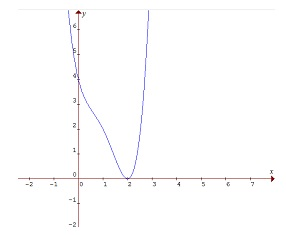
\includegraphics[width=.6\linewidth]{2_elem_rekenvaardigheden_B/inputs/veeltermfuncties4.jpg} 
\caption{Veeltermfuncties: voorbeeld 4.}
\label{fig:vt:vb4}
\end{figure}


\textbf{Tekenverloop}

Maak \'e\'en overzichtelijke tabel met bovenaan alle nulpunten
in stijgende volgorde. Per rij onderzoek je het teken van elke factor
van $f(x)$. Het teken van $f(x)$ is dan het product van deze tekens.

\begin{center}
\begin{tabular}{c||c|c|c}
$x$ &  & $2$ & \\
\hline 
$(x-2)^{2}$ & $+$ & $0$ & \multicolumn{1}{c}{$+$}\\
$(x^{2}+1)$ & +&+&+\\
\hline 
$f(x)$ & $+$ & $0$ & $+$\\
\end{tabular}
\par\end{center}

%\subsection{Rationale functies}

\begin{definitie}
	Functievoorschrift

${\displaystyle f(x)=\frac{t(x)}{n(x)}}$ met $t(x)$ en $n(x)$ veeltermfuncties
en waarbij de graad van $n(x)$ minstens 1 is.
\end{definitie}

\begin{voorbeeld}
Voorbeelden van rationale functies: ${\displaystyle f(x)=\frac{x^{2}}{1+x}}$,
${\displaystyle f(x)=\frac{1}{x^{2}-1}}$, ${\displaystyle f(x)=\frac{3x-9}{x-3}}$

Voorbeelden van niet-rationale functies: ${\displaystyle f(x)=\frac{\sin x}{4x}}$,
${\displaystyle f(x)=\frac{2^{x}}{3x+5}}$, ${\displaystyle f(x)=\frac{\sqrt{x-1}}{x-3}}$

\end{voorbeeld}

\textbf{Grafische voorstelling}

Het domein van een rationale functie is $\mathbb{R\setminus}\textrm{\{nulpunten\:van\:de\:noemer\}}$.

\begin{definitie}
	Voorbeeld: het domein van ${\displaystyle f(x)=\frac{2x+2}{x-8}}$
is ${\displaystyle \mathbb{R}\setminus\{8\}}$
\end{definitie}

\textbf{Nulpunten}

De nulpunten van een rationale functie $f(x)$, zijn de nulpunten
van de teller, die niet de nulpunten van de noemer zijn.

De nulpunten van de noemer, noemen we de polen van de rationale functie
$f(x)$. Bij elke pool hoort een verticale asymptoot.

Punten die zowel nulpunt zijn van teller als noemer, geven aanleiding
tot de vorm $\frac{0}{0}$. Aangezien deze punten de noemer nul maken,
horen ze niet tot het domein, maar geven ook geen aanleiding tot een
asymptoot.


\textbf{Asymptoten}

\begin{enumerate}
\item De rechte $x=a$ is een \textbf{verticale asymptoot} (VA) van de
rationale functie $f(x)$ als en slechts als $a$ een nulpunt is van
de noemer en geen nulpunt van de teller.

\begin{equation*}
\lim_{\overset{x\rightarrow a}{<}}f(x)=\pm\infty\quad\textrm{of}\quad \lim_{\overset{x\rightarrow a}{>}}f(x)=\pm\infty \\
		\Rightarrow\:x=a\:\textrm{is een VA}
\end{equation*}

\begin{voorbeeld}
\ 
\begin{equation*}
f(x)=\frac{2x+1}{x-1}
\end{equation*}

Het nulpunt van de noemer, of de pool is $x=1$. Dit punt is geen
nulpunt van de teller. Dus, $x=1$ is een verticale asymptoot. De
functie $f(x)$ is niet gedefinieerd in het punt $x=1$.
\begin{equation*}
\lim_{\overset{x\rightarrow1}{<}}\left(\frac{2x+1}{x-1}\right)=-\infty\quad\textrm{en}\quad \lim_{\overset{x\rightarrow1}{>}}\left(\frac{2x+1}{x-1}\right)=+\infty
\Rightarrow\:x=1\:\textrm{is een VA}
\end{equation*}

\end{voorbeeld}

\item Een rationale functie $f(x)$ heeft een \textbf{horizontale asymptoot}
(HA) als en slechts als de graad van de teller \ensuremath{\le} graad
van de noemer.

\begin{equation*}
\lim_{x\to\pm\infty}f(x)=b
\Rightarrow\:y=b\:\textrm{is een HA}
\end{equation*}

\begin{voorbeeld}
\ 
\begin{equation*}
f(x)=\frac{2x+7}{4x^{2}+x+2}
\end{equation*}

De graad van de teller is 1, en de graad van de noemer is 2; dus deze
functie heeft een horizontale asymptoot.

\begin{equation*}
\lim_{x\to\pm\infty}\frac{2x+7}{4x^{2}+x+2}\overset{HGT}{=} \lim_{x\to\pm\infty}\frac{2x}{4x^{2}}=\lim_{x\to\pm\infty}\frac{1}{2x}=0
\displaystyle \Rightarrow\:y=0\:\textrm{is een HA}
\end{equation*}

\end{voorbeeld}

\item Een rationale functie $f(x)$ heeft een \textbf{schuine asymptoot}
(SA) als en slechts als de graad van de teller = graad van de noemer
+1.

\begin{equation*}
m=\lim_{x\to\pm\infty}\frac{f(x)}{x}\quad\textrm{en}\quad q=\lim_{x\to\pm\infty}\left[f(x)-mx\right]\Rightarrow\:y=mx+q\:\textrm{is een SA}
\end{equation*}

\begin{voorbeeld}
	\begin{equation*}
f(x)=\frac{x^{3}-4}{2x^{2}}
\end{equation*}

De graad van de noemer is 2, en de graad van de teller is (2+1=) 3,
dus deze functie heeft een schuine asymptoot.

\begin{eqnarray*}
m&=&\lim_{x\to\pm\infty}\frac{f(x)}{x}= \lim_{x\to\pm\infty}\frac{x^{3}-4}{2x^{3}}\overset{HGT}{=} \lim_{x\to\pm\infty}\frac{x^{3}}{2x^{3}}=\frac{1}{2}
\\
q&=& \lim_{x\to\pm\infty}\left[\frac{x^{3}-4}{2x^{2}}-\frac{1}{2}x\right]=\lim_{x\to\pm\infty}\left[\frac{x^{3}-4-x^{3}}{2x^{2}}\right]=0 \\
&&\Rightarrow\:y=\frac{1}{2}x\:\textrm{is een SA}
\end{eqnarray*}

\end{voorbeeld}

\begin{opmerking}
Als een functie $f(x)$ voor $x\rightarrow+\infty$ een
horizontale asymptoot heeft, kan ze voor $x\rightarrow+\infty$ geen
schuine asymptoot meer hebben. Hetzelfde geldt voor $x\rightarrow-\infty$.
\end{opmerking}
\end{enumerate}

\textbf{Tekenverloop}

Om het tekenverloop van een rationale functie te bepalen, moet het
tekenonderzoek van de teller en de noemer worden uitgevoerd. Het tekenverloop
van een constante, een lineaire en een kwadratische functie is gekend
(zie Module 2 sectie \ref{sec:eerste_tweede} en \ref{sec:vtf}).
Het teken van de rationale functie is het product van het teken van
de teller en het teken van de noemer.


\begin{voorbeeld}
Bespreek de rationale functie 
\begin{equation*}
f(x)=\frac{3x^{2}}{x^{2}-2}
\end{equation*}

\underline{Domein}

$\textrm{dom}f(x)=\mathbb{R}\setminus\{-\sqrt{2},\sqrt{2}\}$ want de noemer mag niet nul worden. Dit gebeurt als ${\displaystyle x^{2}-2=0}\Longleftrightarrow x=\pm\sqrt{2}$.

\underline{Nulwaarden}

Stap 1: Bepaal de nulpunten van de teller, deze zijn de nulpunten
van de functie $f(x)$. Dus $3x^{2}=0\Longleftrightarrow x=0$ .

$x=0$ is een nulpunt van de teller, maar niet van de noemer, dus
dit punt is een nulpunt van de functie $f(x)$.

Stap 2: Bepaal de nulpunten van de noemer, deze zijn de polen van
de functie $f(x)$. Bij elke pool hoort een verticale asymptoot.

$x=-\sqrt{2}$ en $x=+\sqrt{2}$ zijn de nulpunten van de noemer,
de functie $f(x)$ heeft dus twee verticale asymptoten.

\underline{Asymptoten}

Stap 3: Ga na of de functie een verticale asymptoot bezit. 

De rechte $x=-\sqrt{2}$ is een verticale asymptoot (VA) van de functie
$f(x)$ aangezien $-\sqrt{2}$ een nulpunt is van de noemer en geen
nulpunt van de teller is.

Hoe verloopt de functie $f(x)$ in de buurt van deze asymptoot:

\begin{equation*}
\textrm{LL}: \lim_{\overset{x\rightarrow-\sqrt{2}}{<}}\left(\frac{3x^{2}}{x^{2}-2}\right)=+\infty\quad\textrm{en}\quad \textrm{RL}:\lim_{\overset{x\rightarrow-\sqrt{2}}{>}}\left(\frac{3x^{2}}{x^{2}-2}\right)=-\infty
\Rightarrow x=-\sqrt{2} \text{is een VA.}
\end{equation*}

De rechte $x=+\sqrt{2}$ is een verticale asymptoot (VA) van de functie
$f(x)$ aangezien $+\sqrt{2}$ een nulpunt is van de noemer en geen
nulpunt van de teller is.

Hoe verloopt de functie $f(x)$ in de buurt van deze asymptoot:

\begin{equation*}
\textrm{LL}: \lim_{\overset{x\rightarrow\sqrt{2}}{<}}\left(\frac{3x^{2}}{x^{2}-2}\right)=-\infty\quad\textrm{en}\quad \textrm{RL}:\lim_{\overset{x\rightarrow\sqrt{2}}{>}}\left(\frac{3x^{2}}{x^{2}-2}\right)=+\infty \\
\Rightarrow x=+\sqrt{2} \text{is een VA.}
\end{equation*}


Stap 4: Ga na of de functie een horizontale asymptoot bezit. De functie
$f(x)$ heeft een horizontale asymptoot (HA) aangezien de graad van
teller (2\textsuperscript{de} graad) = graad van de noemer (2\textsuperscript{de}
graad).

\begin{equation*}
\lim_{x\to\pm\infty}\frac{3x^{2}}{x^{2}-2}\overset{HGT}{=} \lim_{x\to\pm\infty}\frac{3x^{2}}{x^{2}}=3 \\
\Rightarrow y=3\text{ is een HA}.
\end{equation*}

Stap 5: Ga na of de functie een schuine asymptoot heeft. De functie
$f(x)$ heeft voor $x\rightarrow+\infty$ en $x\rightarrow-\infty$,
al een horizontale asymptoot en kan bijgevolg geen schuine asymptoot
meer hebben.

\underline{Tekenverloop}

Stap 6: - Schrijf in \'e\'en tabel bovenaan alle nulpunten en alle polen
in stijgende volgorde. 

\begin{itemize}
\item Onderzoek het teken voor elke factor van $f(x)$ . 
\item Het teken van $f(x)$ is dan het product van deze tekens.
\end{itemize}

\begin{center}
	\begin{tabular}{c||cccccccc} 
$x$ &  & $-\sqrt{2}$ &  & $0$ &  & $-\sqrt{2}$ &  & ${\displaystyle \longrightarrow\mathbb{R}}$\\
\hline 
${\displaystyle 3x^{2}}$ & + &  & + & 0 & + &  & + & \\
\hline 
${\displaystyle x^{2}-2}$ & + & 0 & - & - & - & 0 & + & \\
\hline 
${\displaystyle f(x)=\frac{3x^{2}}{x^{2}-2}}$ & + & $\mid$ & - & 0 & - & $\mid$ & + & \\
\end{tabular}
\end{center}

\underline{Grafiek}

%\gewonefiguur{width=10cm}{2_elem_rekenvaardigheden_B/inputs/vb_rat1}

\begin{figure}
\centering
\input{2_elem_rekenvaardigheden_B/Fig_module_2_1_8_vb_rat1}
\end{figure}


\end{voorbeeld}


\begin{ftonthoud}
	De grafiek en het tekenverloop van een rationale functie bepaal je
als volgt: $f(x)=\frac{t(x)}{n(x)}$ met $t(x)$ en $n(x)$ veeltermfuncties
en waarbij de graad van $n(x)$ minstens 1 is.

Het domein van een rationale functie is $\mathbb{R\setminus}\textrm{\{nulpunten\:van\:de\:noemer\}}$.

Stap 1: Bepaal de nulpunten van de teller, dit zijn de nulpunten van
de functie $f(x)$.

Stap 2: Bepaal de nulpunten van de noemer, dit zijn de polen van de
functie $f(x)$.

Stap 3: De rechte $x=a$ is een \textbf{verticale asymptoot} (VA)
van de rationale functie $f(x)$ als en slechts als $a$ een nulpunt
is van de noemer en maar geen nulpunt van de teller.

\begin{equation*}
\lim_{\overset{x\rightarrow a}{<}}f(x)=\pm\infty\quad\textrm{of}\quad \lim_{\overset{x\rightarrow a}{>}}f(x)=\pm\infty\quad\Rightarrow\:x=a\:\textrm{is een VA}
\end{equation*}


Stap 4: Een rationale functie $f(x)$ heeft een \textbf{horizontale
asymptoot} (HA) als en slechts als de graad van de teller \ensuremath{\le}
graad van de noemer. Maar hou wel rekening met het domein.

\begin{equation*}
\lim_{x\to\pm\infty}f(x)=b\quad\Rightarrow\:y=b\:\textrm{is een HA}
\end{equation*}

Stap 5: Een rationale functie $f(x)$ heeft een \textbf{schuine asymptoot}
(SA) als en slechts als de graad van de teller = graad van de noemer
+1. Maar hou wel rekening met het domein.

\begin{eqnarray*}
m= \lim_{x\to\pm\infty}\frac{f(x)}{x}\quad\textrm{en}\quad
q=\lim_{x\to\pm\infty}\left[f(x)-mx\right] \\
\Rightarrow\:y=mx+q\:\textrm{is een SA}
\end{eqnarray*}

Stap 6: Bepaal het tekenverloop
\begin{itemize}
\item Schrijf in \'e\'en tabel bovenaan alle nulpunten en alle polen in stijgende
volgorde. 

\item Onderzoek het teken voor elke factor van $f(x)$.

\item Het teken van $f(x)$ is dan het product van deze tekens.

\end{itemize}

\end{ftonthoud}

%\subsection{Irrationale functies}
%\maketitle
%\begin{itemize}
%\item Wat zijn irrationale functies?
%\item Wanneer hebben ze (verticale, horizontale en/of schuine) asymptoten?
%\end{itemize}
%Dit zijn vergelijkingen waarin wortelvormen voorkomen, eventueel met
%een breuk. Deze wortelvormen kan je wegwerken door beide leden van
%de vergelijking te verheffen tot een gepaste macht.

\begin{voorbeeld}
	$f(x)=\sqrt{x^{2}+2x+4}$, $f(x)=2\cdot \sqrt[3]{x^{5}-3x^{2}+7}-x-1$,
$f(x)=\frac{x-2}{\sqrt{10-x^{2}}}$
\end{voorbeeld}

\textbf{Grafische voorstelling}

De grafiek van de elementaire wortelfuncties $y=\sqrt[n]{x}$
is hieronder weergegeven. Denk eraan dat (machts)wortels ook als macht
kunnen geschreven worden: $y=\sqrt[n]{x}=x^{\frac{1}{n}}$.

\gewonefiguur{width=10cm}{2_elem_rekenvaardigheden_B/inputs/machtsw1}

Om het domein (de toegelaten waarden voor $x$) te bepalen moeten
we rekening houden met zowel de \emph{bestaansvoorwaarden} als de
\emph{kwadrateringsvoorwaarde}.

\begin{itemize}
	\item Bestaansvoorwaarde(n): de uitdrukking onder een even machtswortel
moet steeds positief zijn!! En niet vergeten, de eventuele noemer
mag niet nul worden.
\item Kwadrateringsvoorwaarde: we spreken af dat een even machtswortel uit
een uitdrukking steeds positief is.
\end{itemize}

Het domein van een irrationale functie valt samen met de intervallen,
waar de vorm onder de vierkantswortel niet negatief is en waar de
uitdrukking van een even machtsfunctie steeds een positief resultaat
oplevert.

\begin{voorbeeld}
	\begin{equation*}
f(x)=\sqrt{x^{2}-4}
\end{equation*}

\gewonefiguur{width=7cm}{2_elem_rekenvaardigheden_B/inputs/machtsw2}

Om het domein van de functie $f(x)$ te bepalen moet er aan de bestaansvoorwaarde(n)
voldaan zijn. In dit geval mag de functie onder het wortelteken niet
negatief worden. We werken dit verder uit:

De bestaansvoorwaarde: $\begin{array}{cccl}
x^{2}-4\geq0 &\iff & x^{2}\geq4\\
& \iff & x\geq2 \textrm{ en } x\leq-2
\end{array}$

De kwadrateringsvoorwaarde is reeds voldaan (want er staat infeite
$f(x)=+\sqrt{x^{2}-4}$).

Welke waarden van $x$ voldoen hier nu aan? $\textrm{dom}f(x)$ is voor $x\in]-\infty,-2]\bigcup[2,+\infty[$.

\end{voorbeeld}

\begin{voorbeeld}
\begin{equation*}
f(x)=x+\sqrt{5x+2}-1
\end{equation*}

\gewonefiguur{width=7cm}{2_elem_rekenvaardigheden_B/inputs/vbirrat1}

Om het domein van de functie $f(x)$ te bepalen moet er aan de bestaansvoorwaarde(n)
voldaan zijn. In dit geval mag de functie onder het wortelteken niet
negatief worden. We werken dit verder uit:

De bestaansvoorwaarde:$\begin{array}{cclccc}
 & 5x+2\geq0
 & \iff & x & \geq & -\frac{2}{5}\\
\textrm{dus} & & \iff & x & \in & [-\frac{2}{5},+\infty[
\end{array}$

Nu moeten we nog de kwadrateringsvoorwaarde controleren, m.a.w. volgens
onze gemaakte afspraak is een even machtswortel uit een uitdrukking
steeds positief is:

De bestaansvoorwaarde:
$\begin{array}{cccclcc}
 & x+\sqrt{5x+2}=1 & \iff & \sqrt{5x+2} & = & 1-x & \geq0\\
 & & \iff & 1-x & \geq & 0\\
\textrm{dus} & & \iff & x & \leq & 1\\
\textrm{of} & & \iff & x & \in & ]-\infty,1]
\end{array}$

De mogelijke waarden voor $x$ moeten aan beide voorwaarden voldoen.
Dit betekent: $\textrm{dom}f(x)$ is voor $x\in[-\frac{2}{5},1]$

\end{voorbeeld}

\textbf{Nulpunten}

De vergelijking wordt $f(x)=0$.

De wortelvormen kan je wegwerken door beide leden van de vergelijking
te verheffen tot een gepaste macht. Bepaal vervolgens de nulpunten
van de functie. Wanneer een breuk voorkomt in het functievoorschrift,
bepaal dan ook de nulpunten van de noemer, deze zijn de polen.

\textbf{Asymptoten}

\begin{enumerate}
	\item De rechte $x=a$ is een \textbf{verticale asymptoot} (VA) van de
irrationale functie $f(x)$ als en slechts als $a$ een nulpunt is
van de noemer en geen nulpunt van de teller.

\begin{equation*}
\lim_{\overset{x\rightarrow a}{<}}f(x)=\pm\infty\quad\textrm{of}\quad \lim_{\overset{x\rightarrow a}{>}}f(x)=\pm\infty \Rightarrow\:x=a\:\textrm{is een VA}
\end{equation*}

\item Een irrationale functie $f(x)$ heeft een \textbf{horizontale asymptoot}
(HA) als en slechts als de graad van de teller $\le$ graad
van de noemer.
\begin{equation*}
\lim_{x\to\pm\infty}f(x)=b \Rightarrow\:y=b\:\textrm{is een HA}
\end{equation*}

\item Een irrationale functie $f(x)$ heeft een \textbf{schuine asymptoot}
(SA) als en slechts als de graad van de teller = graad van de noemer
+1.

\begin{equation*}
m=\lim_{x\to\pm\infty}\frac{f(x)}{x}\quad\textrm{en}\quad 
q= \lim_{x\to\pm\infty}\left[f(x)-mx\right]
\Rightarrow\:y=mx+q\;\textrm{is een SA}
\end{equation*}

\end{enumerate}


\textbf{Tekenverloop}

Wanneer je de wortels hebt weggewerkt door de vergelijking te verheffen
tot een gepaste macht, zal je een veeltermfunctie, een kwadratische
of een lineaire functie bekomen. Pas het desbetreffend tekenonderzoek
toe.


\begin{voorbeeld}
	Bespreek de irrationale functie $f(x)=\frac{\sqrt{4-x^{2}}}{x-1}$

\underline{Domein}

\begin{eqnarray}
\textrm{dom}f(x)=[-2,1[\bigcup]1,2]
\end{eqnarray}

want de bestaansvoorwaarden zijn:  
\begin{equation*}
\begin{array}{ccclcc}
& 4-x^{2}\geq0 & \iff & x^{2}\leq4\\
\textrm{dus} & & \iff & x\leq2\;\textrm{en}\:x\geq-2\\
\textrm{of} & & \iff & x\in[-2,2]
\end{array}
\end{equation*}

en:
\begin{equation*}
x-1\neq0 \textrm{ dus } x\neq1
\end{equation*}

De kwadrateringsvoorwaarde is hier niet van toepassing (vanwege de
noemer kan $f(x)$ ook negatief worden).

\underline{Nulpunten}

Stap 1: Bepaal de nulpunten van de teller, deze zijn de nulpunten
van de functie $f(x)$.

Dus 
\begin{equation*}
\begin{array}{ccc}
f(x)=0 & \iff & \frac{\sqrt{4-x^{2}}}{x-1} = 0\\
& \iff & \sqrt{4-x^{2}} = 0\\
& \iff & 4-x^{2} = 0\\
& \iff & x^{2} = 4\\
& \iff & x = \pm2
\end{array}
\end{equation*}

Stap 2: Bepaal eventueel de nulpunten van de noemer, deze zijn de
polen van de functie $f(x)$. Bij elke pool hoort een verticale asymptoot.

Het nulpunt van de noemer is $x=1$ (dit is dan tevens de vergelijking
van de verticale asymptoot).

\underline{Asymptoten}

Stap 3: Ga na of de functie een verticale asymptoot bezit. 

De rechte $x=1$ is een verticale asymptoot (VA) van de functie $f(x)$
aangezien $1$ een nulpunt is van de noemer en geen nulpunt van de
teller is.

Hoe verloopt de functie $f(x)$ in de buurt van deze asymptoot:

\begin{equation*}
\textrm{LL}:\lim_{\overset{x\rightarrow1}{<}}\left(\frac{\sqrt{4-x^{2}}}{x-1}\right)=-\infty\quad\textrm{en}\quad \textrm{RL}:\lim_{\overset{x\rightarrow1}{>}}\left(\frac{\sqrt{4-x^{2}}}{x-1}\right)=+\infty \Rightarrow x=1 \text{ is een VA}
\end{equation*}


Stap 4: Ga na of de functie een horizontale asymptoot bezit.

De functie heeft geen horizontale asymptoot, want $x$ die nadert
naar $+\infty$ of $-\infty$ behoort niet tot het domein.

Stap 5: Ga na of de functie een schuine asymptoot heeft.

De functie heeft geen schuine asymptoot, want $x$ die nadert naar
$+\infty$ of $-\infty$ behoort niet tot het domein.

\underline{Tekenverloop}

Stap 6:
\begin{itemize}
\item Schrijf in \'e\'en tabel bovenaan alle nulpunten en alle polen
	in stijgende volgorde. 
\item Onderzoek het teken voor elke factor van $f(x)$. 
\item Het teken van $f(x)$ is dan het product van deze tekens.
\end{itemize}


\begin{tabel}{Voorbeeld irrationale functies: tekenverloop.}
\begin{tabular}{c|cccccccc}
$x$ &  & $-2$ &  & $1$ &  & $2$ &  & $\longrightarrow\mathbb{R}$\\
\hline  
$\sqrt{4-x^{2}}$ & / & 0 & + &  & + & 0 & / & \\
$x-1$ & - & - & - & 0 & + & + & + & \\
\hline 
$f(x)=\frac{\sqrt{4-x^{2}}}{x-1}$ & / & 0 & - & $\mid$ & + & 0 & / & \\
\end{tabular}
\label{tab:irrattk}
\end{tabel}

\underline{Grafiek}

\gewonefiguur{width=7cm}{2_elem_rekenvaardigheden_B/inputs/vbirrat2}

\end{voorbeeld}

\begin{ftonthoud}
	De grafiek en het tekenverloop van een irrationale functie bepaal
je als volgt:

Het domein van een irrationale functie valt samen met de intervallen,
waar de vorm onder de vierkantswortel niet negatief (BVW) is en waar
de uitdrukking van een even machtsfunctie steeds een positief resultaat
oplevert (KVW).

Stap 1: Bepaal de nulpunten van de teller, dit zijn de nulpunten van
de functie $f(x)$.

Stap 2: Bepaal eventueel de nulpunten van de noemer, dit zijn de polen
van de functie $f(x)$.

Stap 3: De rechte $x=a$ is een \textbf{verticale asymptoot} (VA)
van de irrationale functie $f(x)$ als en slechts als $a$ een nulpunt
is van de noemer en maar geen nulpunt van de teller.

\begin{equation*}
\lim_{\overset{x\rightarrow a}{<}}f(x)=\pm\infty\quad\textrm{of}\quad \lim_{\overset{x\rightarrow a}{>}}f(x)=\pm\infty\quad\Rightarrow\:x=a\:\textrm{is een VA}
\end{equation*}

Stap 4: Een irrationale functie $f(x)$ heeft een \textbf{horizontale
asymptoot} (HA) als en slechts als de graad van de teller \ensuremath{\le}
graad van de noemer.
\begin{equation*}
 \lim_{x\to\pm\infty}f(x)=b\quad\Rightarrow\:y=b\:\textrm{is een HA}
\end{equation*}


Stap 5: Een irrationale functie $f(x)$ heeft een \textbf{schuine
asymptoot} (SA) als en slechts als de graad van de teller = graad
van de noemer +1.

\begin{equation*}
m=\lim_{x\to\pm\infty}\frac{f(x)}{x}\quad\textrm{en}\quad q= \lim_{x\to\pm\infty}\left[f(x)-mx\right] \Rightarrow\:y=mx+q\:\textrm{is een SA}
\end{equation*}


Stap 6: Bepaal het tekenverloop

\begin{itemize}
\item Schrijf in \'e\'en tabel bovenaan alle nulpunten en alle polen in stijgende
volgorde.

\item Hou rekening met de bestaansvoorwaarde en de kwadrateringsvoorwaarde.

\item Onderzoek het teken voor elke factor van $f(x)$.

\item Het teken van $f(x)$ is dan het product van deze tekens.
\end{itemize}

\end{ftonthoud}
%%\DeclareMathOperator{\tri}{tri} \DeclareMathOperator{\rect}{rect}
%\DeclareMathOperator{\sgn}{sgn} \DeclareMathOperator{\ramp}{ramp}
%\DeclareMathOperator{\sinc}{sinc}


\subsection{Exponenti\"ele functies}
%\maketitle
%\begin{itemize}
%\item Wat is een exponenti\"ele functie?
%\item Hoe ziet het functievoorschrift van een exponenti\"ele functie eruit?
%\item Welke rekenregels voor machten en wortels zijn er?
%\item Hoe lossen we exponenti\"ele vergelijkingen op?
%\item Hoe kan je een exponenti\"ele functie grafisch voorstellen?
%\item Hoe bepaal je het tekenverloop van een exponenti\"ele functie? 
%\end{itemize}


\begin{definitie}
De exponenti\"ele functie is van de vorm:
\begin{equation*}
	y=a^{x}\text{ met }a\in\mathbb{R}_{0}^{+}\setminus\{ 1\}\text{ en }x\in\mathbb{R}
\end{equation*}
$a$ noemen we het \textbf{grondtal}, en moet strikt positief
en verschillend van 1 zijn.

$x$ noemen we de \textbf{exponent}, en is een re\"eel getal.
\end{definitie}

\begin{voorbeeld}
\begin{eqnarray*}
4^{2}&=&16 \\
3^{-2}&=&\frac{1}{3^{2}}=\frac{1}{9} \\
5^{\frac{2}{3}}&=&\sqrt[3]{5^{2}} \\
5^{-\frac{3}{2}}&=&\frac{1}{5^{\frac{3}{2}}}=\frac{1}{\sqrt{5^{3}}}=\frac{1}{\sqrt{5^{2}.5}}=\frac{1}{5\sqrt{5}}\\
\sqrt{25}&=&5 \\
\sqrt[4]{10000}&=&10\\
\sqrt[5]{-32}&=&-2\\
\sqrt[3]{8}&=&2\\
\end{eqnarray*}
\end{voorbeeld}

\begin{opmerking}
De positieve tweedemachts- of vierkantswortel van 25 is 5, want $5>0$ en $5^{2}=25$, dit wordt genoteerd als ${\displaystyle \sqrt{25}=5}$.

En de negatieve tweedemachts- of vierkantswortel van 25 is -5, want
$-5 < 0$ en $(-5)^{2}=25$, dit wordt genoteerd als ${\displaystyle -\sqrt{25}=-5}$.

Ook je rekenmachine zal bij ${\displaystyle \sqrt{25}}$ als resultaat
5 geven. Verwar dit niet met het oplossen van de vergelijking $x^{2}=25$.
In dit geval zijn de twee oplossingen van de vergelijking: $x=\pm\sqrt{25}=\pm5$.
\end{opmerking}

\subsubsection{Bijzondere gevallen}
\begin{itemize}
\item De exponenti\"ele functie met grondtal $e$ ($e=2,718281828$) wordt
genoteerd als $y=e^{x}$.
\item $a^{0}=1$
\item $a^{1}=a$
\item Als n even is spreekt men van een \emph{evenmachtswortel} ($\sqrt{\ }$,
$\sqrt[4]{\ }$, ...), is n oneven dan spreekt men van een \emph{onevenmachtswortel}
($\sqrt[3]{\ }$, $\sqrt[5]{\ }$, ...).
\item Positieve re\"ele getallen hebben twee tegengestelde evenmachtswortels
en juist \'e\'en positieve onevenmachtswortel.
\item als n even is, dan heeft elk re\"eel getal $a$ twee n\textsuperscript{de}
machtswortels die tegengesteld zijn, genoteerd door $-\sqrt[n]{a}$
en $+\sqrt[n]{a}$, of kortweg $\pm\sqrt[n]{a}$.
\item als n oneven is, dan heeft elk re\"eel getal a juist \'e\'en n\textsuperscript{de}
machtswortel, genoteerd door $\sqrt[n]{a}$.
\item Als n even is, dan hebben de negatieve getallen geen n\textsuperscript{de}
machtswortel; dus negatieve re\"ele getallen hebben geen (re\"ele) evenmachtswortel
en juist \'e\'en onevenmachtswortel welke negatief is.
\end{itemize}
Let op: worteltrekken is niet hetzelfde als het oplossen van een vergelijking:

\begin{tabel}{}
\begin{tabular}{c|c}
worteltrekken & vergelijking oplossen\\
\hline 
$\sqrt{4}=2$ & $\begin{array}{lll}
x^{2} & = & 4\\
x & = & \pm\sqrt{4}\\
x & = & \pm2
\end{array}$\\
\hline 
 &  $x_{1}=-2$ en $x_{2}=+2$\\
\end{tabular}
\end{tabel}


\subsubsection{Rekenregels}

\begin{tabel}{}
\begin{tabular}{l|l}
machten & wortels\\
\hline 
$a^{m}a^{n}=a^{m+n}$ & $\sqrt[m]{a}\cdot\sqrt[n]{a}=\sqrt[m\cdot n]{a^{m+n}}$\\
$\frac{a^{m}}{a^{n}}=a^{m-n}$ & $\sqrt[n]{a^{m}}=a^{\frac{m}{n}}$\\
$\left(\frac{1}{a}\right)^{n}=a^{-n}$ & $\sqrt[n]{a}=a^{\frac{1}{n}}$\\
$\left(a^{m}\right)^{n}=a^{m\cdot n}$ & $\sqrt[n]{\sqrt[m]{a}}=\sqrt[n\cdot m]{a}$\\
$\left(a\cdot b\right)^{n}=a^{n}\cdot b^{n}$ & $\sqrt[n]{a\cdot b}=\sqrt[n]{a}\cdot \sqrt[n]{b}$\\
$\left(\frac{a}{b}\right)^{n}=\frac{a^{n}}{b^{n}}$ & $\sqrt[n]{\frac{a}{b}}=\frac{\sqrt[n]{a}}{\sqrt[n]{b}}$\\
\end{tabular}
\end{tabel}


\begin{opmerking}
	\ \\
	\begin{itemize}
\item aangezien $1=\frac{a}{a}=a^{1-1}=a^{0}$ zie je waarom
we zeggen dat $a^{0}=1$.
\item formules met wortels kan je (gemakkelijk) terugvinden als je de wortelvorm
herschrijft d.m.v. machten:
\end{itemize}
\begin{equation*}
\sqrt[m]{a}.\sqrt[n]{a}=a^{\frac{1}{m}}.a^{\frac{1}{n}}=a^{\frac{1}{m}+\frac{1}{n}}=a^{\frac{m+n}{m.n}}=\sqrt[m.n]{a^{m+n}}
\end{equation*}
\begin{itemize}
\item laat je niet vangen: $\sqrt{a+b}\neq\sqrt{a}+\sqrt{b}$
\item een veel gebruikte bewerking is het wortelvrij maken van de noemen,
bv.: $\frac{1}{\sqrt{2}}=\frac{1}{\sqrt{2}}.\frac{\sqrt{2}}{\sqrt{2}}=\frac{\sqrt{2}}{2}.$
\end{itemize}
\end{opmerking}

\subsubsection{Oplossen van exponenti\"ele vergelijkingen}

Algemeen

In sommige opgaves kom je exponenti\"ele vergelijkingen tegen. Dit zijn
vergelijkingen waar de onbekende voorkomt in de exponent. Om exponenti\"ele
vergelijkingen vlot te kunnen oplossen, maak je best gebruik van onderstaand
stappenplan:

Stap 1: Noteer de vergelijking in haar standaardvorm: $ a^{f(x)}=c$
of $ a^{f(x)}=a^{g(x)}$ of $ a^{f(x)}=b^{g(x)}$ 

Stap 2: Laat op beide leden van de vergelijking een geschikte logaritmische
functie inwerken.

Stap 3: Stop de uitkomst in de opgave en controleer.

\begin{voorbeeld}

Los op: $8^{x-1}-4=0$
\begin{equation*}
 \begin{array}{rclr}
 8^{x-1}-4=0 &
	\iff & 8^{x-1} = 4 & \text{ (stap 1)}\\
	& \iff & 2^{3x-3} = 2^{2} & \text{ (zoek een verband tss 8, 4 en 2)}\\
	& \iff & \log2^{3x-3} = \log2^{2} & \text{ (stap 2)}\\
	& \iff & 3x-3 = 2 & \text{}\\
	& \iff & x = \frac{5}{3}
	\end{array}
\end{equation*}

In stap 3 controleer je dat $ 8^{\frac{5}{3}-1}-4=0$?
Dit is ok.

Opmerking: stap 2 kan je ook in gedachten doen, m.a.w. hoef je niet
op te schrijven.

\end{voorbeeld}
\begin{voorbeeld}
	
\begin{equation*}
a^{f(x)}=b^{g(x)}
\end{equation*}

Los op: $50\sqrt{0,1^{x}}=10^{x+1}\sqrt{2,5}$

\begin{equation*}
 \begin{array}{rclr}
 50\sqrt{0,1^{x}}=10^{x+1}\sqrt{2,5} & 
	\iff & 50.\left(0,1\right)^{\frac{x}{2}} = 10^{x+1}\sqrt{2,5} & \text{ (stap 1)}\\
	&\iff & 50.10^{-\frac{x}{2}} = 10^{x}.10.\sqrt{2,5} & \text{ (zoek een verband tss 0,1 en 10)}\\
	&\iff & 10^{-\frac{x}{2}}.10^{-x} = \frac{10.\sqrt{2,5}}{50} & \textrm{(zet alle factoren met x bij elkaar)}\\
	&\iff & 10^{-\frac{3}{2}x} = \sqrt{\frac{100.2,5}{2500}}\\
	&\iff & \log10^{-\frac{3}{2}x} = \log10^{-\frac{1}{2}} & \text{ (stap 2)}\\
	&\iff & -\frac{3}{2}x = -\frac{1}{2} & \text{}\\
	&\iff & x = \frac{1}{3} & 
	\end{array}
\end{equation*}

In stap 3 controleer je dat $ 50\sqrt{0,1^{\frac{1}{3}}}=10^{\frac{1}{3}+1}\sqrt{2,5}$? Dit is ok.

Opmerking: stap 2 kan je ook in gedachten doen, m.a.w. hoef je niet
op te schrijven.
\end{voorbeeld}


\begin{voorbeeld}
Los op:  \begin{equation*}
2^{2x}-3\cdot 2^{(x+2)}+36=0
\end{equation*}

\begin{equation*}
 \begin{array}{lr}
 2^{2x}-3\cdot 2^{(x+2)}+36 = 0 & \\
	 2^{2x}-3\cdot 2^{x}\cdot 2^{2}+36 = 0 & \\
	 2^{2x}-12\cdot 2^{x}+36 = 0 & \text{ (herken dat \ensuremath{ 2^{2x}=\left(2^{x}\right)^{2}}}) \\
 	 & \text{ stel }2^{x}=t\\
	 t^{2}-12\cdot t+36 = 0 & \text{ (los de vierkantsvgl op)}
	\end{array}
\end{equation*}

\begin{equation*}
t_{1\textrm{en}2}=\frac{-(-12)\pm\sqrt{(-12)^{2}-4\cdot 1\cdot 36}}{2\cdot 1}=\frac{12\pm0}{2}=6
\end{equation*}

We zoeken niet $ t_{1\textrm{en}2}$ maar wel de waarde van $x$. Dus: $ 2^{x}=t=6$ zodat $ x=\log_{2}6$.

Ook hier kan je terug controleren of de gevonden waarde van $x$ voldoet
aan de gegeven vergelijking. 

Merk op dat in dit geval hier $ t_{1}$ en $ t_{2}$ gelijk zijn, waardoor er slechts \'e\'en $x$-waarde is. Indien $ t_{1}\neq t_{2}$ dan vind je ook een $x_{1}$ en $ x_{2}$.

Tenslotte, als je een $t$-waarde vindt die negatief is, dan... bestaat
de bijhorende $x$-waarde niet. Je kan immer geen logaritme nemen
van een negatief getal.

\end{voorbeeld}

\subsubsection{De exponenti\"ele functie}

Grafische voorstelling
\begin{itemize}
	\item Het domein van de exponenti\"ele functie is $\mathbb{R}$.
	\item Het beeld van de exponenti\"ele functie is ${\displaystyle \mathbb{R}}_{0}^{+}$,
	dus alle strikt positieve getallen; de grafiek ligt boven de $x$-as.
	\item De punten $(0,1)$ en $(1,a)$ behoren steeds tot de exponenti\"ele
	functie ${\displaystyle f(x)=a^{x}}$.
	\item Als het grondtal $a>1$ is het een stijgende functie.
	\item Als het grondtal $0<a<1$ is het een dalende functie.
	\item De grafieken ${\displaystyle y=a^{x}}$ en ${\displaystyle y=\left(\frac{1}{a}\right)^{x}=a^{-x}}$
	zijn elkaars spiegelbeeld t.o.v. de $y$-as.
\end{itemize}
\gewonefiguur{width=7cm}{2_elem_rekenvaardigheden_B/inputs/exp}

Nulpunten
\begin{itemize}
	\item Er zijn geen nulpunten. De exponenti\"ele functie heeft geen snijpunten
	met de $x$-as. De $x$-as is de horizontale asymptoot.
	\item Het punt $(0,1)$ is het enige snijpunt met de $y$-as.
\end{itemize}

Tekenverloop

\begin{itemize}
	\item Alle functiewaarden $f(x)$ zijn strikt positief, de grafiek ligt
	overal boven de $x$-as.
\end{itemize}

\begin{voorbeeld}
$y=2^{x}$

Grafische voorstelling (stap1):
het grondtal is 2, en $2>0$,
dus krijgen we een stijgende functie. Het punt $(1,a)$ is hier dus
$(1,2)$ en behoort tot de functie ${\displaystyle y=2^{x}}$.


Nulpunten (stap2):
er zijn geen nulpunten. De $x$-as
wordt nooit gesneden. De $x$-as is de horizontale asymptoot. De $y$-as
wordt gesneden in het punt $(0,1)$.


Tekenverloop (stap3) %

\begin{tabel}{}
\begin{tabular}{c|c}
	$x$ & $\longrightarrow\mathbb{R}$\\
	\hline 
	\multirow{1}{*}{$2^{x}$} & + \\
\end{tabular}

\end{tabel}

Grafiek (stap4) 

\gewonefiguur{width=7cm}{2_elem_rekenvaardigheden_B/inputs/vbexp}

\end{voorbeeld}


%
%\DeclareMathOperator{\tri}{tri} \DeclareMathOperator{\rect}{rect}
%\DeclareMathOperator{\sgn}{sgn} \DeclareMathOperator{\ramp}{ramp}
%\DeclareMathOperator{\sinc}{sinc}

\subsection{Logaritmische functies}

%\begin{itemize}
%\item Wat is een logaritmische functie?
%\item Hoe ziet het functievoorschrift van een logaritmische functie eruit?
%\item Welke rekenregels voor logaritmen zijn er?
%\item Hoe lossen we logaritmische vergelijkingen op?
%\item Hoe kan je een logaritmische functie grafisch voorstellen?
%\item Hoe bepaal je het tekenverloop van een logaritmische functie? 
%\end{itemize}

\begin{definitie}
	De logaritmische functie wordt gedefinieerd als de inverse
van de exponenti\"ele functie.

De logaritmische functie is van de vorm:

\begin{equation}
 y=\log_{a}\left(x\right)=\sideset{^{a}}{\left(x\right)}\log\quad\iff\quad a^{y}=x
\end{equation}
met $a\in\mathbb{R}_{0}^{+}\setminus\left\{ 1\right\}$
en $x\in\mathbb{R}_{0}^{+}$

$a$ noemen we het \textbf{grondtal}, en moet strikt positief
en verschillend van 1 zijn. $x$ is een strikt positief re\"eel getal.
\end{definitie}


Om de waarde van $y$ te vinden, stel je jezelf de vraag: ``tot
welke macht moet ik het grondtal $a$ verheffen om $x$ uit te komen?''

\figuurmetlabel[\label{fig:loggraf}]{width=\linewidth}{2_elem_rekenvaardigheden_B/inputs/logExp}{Grafische voorstelling va $y=\log_{10}\left(x\right)=\log(x)$ (links) en $y=\log_{e}\left(x\right)=\ln(x)$ (rechts).}


$\log_{a}(x)$ is de inverse functie van
de functie $a^{x}$; beide functies zijn elkaar spiegelbeeld
t.o.v. de eerste bissectrice ($y=x$).

$\ln(x)$ is de inverse functie van de functie
$e^{x}$; beide functies zijn elkaar spiegelbeeld
t.o.v. de eerste bissectrice ($y=x$).



\begin{voorbeeld}
	\begin{eqnarray*}
\log_{10}\left(100\right)&=&2 \text{ (want $10^{2}=100$)}\\
\log_{2}8&=&3\\
\log_{4}16&=&2\\
\log_{3}9&=&2\\
\log_{3}\sqrt{3}&=&\log_{3}3^{\frac{1}{2}}=\frac{1}{2}\\
\log_{5}\frac{1}{5}&=&\log_{5}5^{-1}=-1
	\end{eqnarray*}
\end{voorbeeld}


\subsubsection{Bijzondere gevallen}
\begin{itemize}
\item De \textbf{tiendelige of Briggse logaritme} is de logaritme met grondtal
10. In de notatie wordt vaak het grondtal 10 weggelaten: $y=\log_{10}\left(x\right)=\log\left(x\right)$
\item De \textbf{natuurlijke of Neperiaanse logaritme} is de logaritme met
grondtal e (e=2,718281828) en wordt genoteerd als $y=\log_{e}(x)$. Ook hier wordt het grondtal e weggelaten, en gebruikt men de specifieke
notatie: $y=\ln(x)$
\item $\log_{a}\left(a\right)=1$ (want $a^{1}=a$)
\item $\log_{a}\left(1\right)=0$ (want $a^{0}=1$)
\item $\log_{a}\left(0\right)$ en $\log_{a}\left(-...\right)$
bestaan niet!
\end{itemize}

\subsubsection{Rekenregels}

\begin{ftrekenregel}
\begin{eqnarray}
\log\left(x.y\right)=\log x+\log y\\
\log\left(\frac{x}{y}\right)=\log x-\log y\\
\log\left(x^{n}\right)=n\log x\\
\log\left(\sqrt[n]{x}\right)=\frac{1}{n}\log x\\
\log_{a}\left(b\right)=\frac{1}{\log_{b}\left(a\right)}\\
\end{eqnarray}
\end{ftrekenregel}


\begin{opmerking}
	\ \\
\begin{itemize}
\item voor de eenvoud hebben we enkele keren het grondtal weggelaten. 
\item laat je niet verleiden, er bestaat geen eenvoudige formule voor $\log\left(x+y\right)=\ldots$
\item $\log\left(x^{n}\right)=\log\left(x\cdot x\cdot x\cdot \:\ldots\:x\right)=\log x+\log x+\:\ldots\:+\log x=n\log x$.
Toch niet zo moeilijk h\'e!?
\item om een logaritme met grondtal $a$ om te zetten naar een logaritme met
grondtal $c$ maken we gebruiken van de volgende eigenschap: $\log_{a}x=\frac{\log_{c}x}{\log_{c}a}$
Hiermee vind je trouwens ook gemakkelijk het laatste rekenregeltje.
Stel, je moet uitrekenen hoeveel $\log_{2}8$ is door
over te gaan op een ander grondtal (bijvoorbeeld 10, wat immers op
je rekentoestel staat). Dan is $\log_{2}8=\frac{\log_{10}8}{\log_{10}2}=\frac{\log8}{\log2}=\frac{0,9031}{0,3010}=3,000$
(en dat hadden we natuurlijk ook al lang uit het hoofd uitgerekend
via een andere eigenschap).
\item soms is het nodig om de variabele $x$ of een getal, op een andere
manier te schrijven. Zowel de notatie $x=10^{log_{10}(x)}$
als $x=\log_{10}10^{x}$ worden regelmatig gebruikt.
Hetzelfde geldt voor $x=e^{log_{e}(x)}=e^{\ln x}$
en $x=\log_{e}e^{x}=\ln e^{x}$. Het idee hierachter
is dat de logaritmische en exponenti\"ele functies elkaars inverse zijn,
waardoor ze elkaar opheffen als ze na elkaar worden toegepast op $x$.
Maar let wel op met bijvoorbeeld $\sqrt{x^{2}}\neq x$
maar wel $\sqrt{x^{2}}=\left|x\right|$(zie ook Module
1 - Absolute waarde).
\end{itemize}

\end{opmerking}

\subsubsection{Oplossen van logaritmische vergelijkingen}

In sommige opgaves kom je logaritmische vergelijkingen tegen. Dit
zijn vergelijkingen waar de onbekende voorkomt in een logaritmische
functie. Om logaritmische vergelijkingen vlot te kunnen oplossen,
maak je best gebruik van onderstaand stappenplan:

Stap 1: Noteer de vergelijking in haar standaardvorm: $ \log_{a}\left(f(x)\right)=c$
of $ \log_{a}\left(f(x)\right)=\log_{a}\left(g(x)\right)$.

Stap 2: Laat op beide leden van de vergelijking een geschikte exponenti\"ele
functie inwerken.

Stap 3: Controleer of de bekomen oplossingen voldoen aan de voorwaarden:
\begin{itemize}
	\item het grondtal moet strikt positief zijn, en verschillend van 1 zijn,
	en
	\item de $ \log_{a}\left(f(x)\right)$ bestaat enkel als
	$ f(x)>0$ . 
\end{itemize}
Stap 4: Stop de uitkomst in de opgave en controleer.


\begin{voorbeeld} $\log_{a}\left(f(x)\right)=\log_{a}\left(g(x)\right)$ 

Los op: $ \log_{3}(x+4)+\log_{3}(x-2)=2\log_{3}x$

\begin{equation*} 
\begin{array}{rclr}
\log_{3}(x+4)+\log_{3}(x-2)=2\log_{3}x
	&\iff & \log_{3}\left[\left(x+4\right)\left(x-2\right)\right] = \log_{3}x^{2} & \text{(stap 1)}\\
	&\iff & 3^{\log_{3}\left[\left(x+4\right)\left(x-2\right)\right]} = 3^{\log_{3}x^{2}} & \text{ (stap 2)}\\
	&\iff & \left(x+4\right)\left(x-2\right) = x^{2} & \\
	&\iff & x^{2}-2x+4x-8 = x^{2} & \\
	&\iff & 2x-8 = 0& \\
	&\iff & x = 4 & 
\end{array}
\end{equation*}


In stap 3 controleren we de voorwaarden voor $x=4$:

\begin{enumerate}
	\item Voor $ \log_{3}(x+4)$ moet gelden: $x+4>0$ $\iff$
$x>-4$? ok.
	\item 2) Voor $ \log_{3}(x-2)$ moet gelden: $x-2>0$ $\iff x>2$? ok.
	\item Voor $ 2\log_{3}x$ moet gelden: $x>0$ ? ok.
\end{enumerate}

Besluit: de oplossing $x=4$ voldoet aan de voorwaarden, en is dus
een oplossing van de vergelijking.

Stap 4: controleer je oplossing: $\log_{3}(4+4)+\log_{3}(4-2)=2\log_{3}4$? ok.

Opmerking: stap 2 kan je ook in gedachten doen, m.a.w. hoef je niet
op te schrijven.
\end{voorbeeld}

\begin{voorbeeld}
$ \log_{a}\left(f(x)\right)=c$

Los op: $ \log_{(x+3)}(x+5)=2$

\begin{equation*}
 \begin{array}{rclr}
 \log_{(x+3)}(x+5)=2 & 
	\iff & (x+3)^{2} = x+5 & \text{(stap 1)} \\
	& & & \textrm{definitie:}\: y=\log_{a}x\Leftrightarrow a^{y}=x\\
	&\iff & x^{2}+6x+9 = x+5 & \text{}\\
	&\iff & x^{2}+5x+4 = 0 & 
	\end{array}
\end{equation*}


\begin{equation*}
x_{1\textrm{en}2}=\frac{-5\pm\sqrt{5^{2}-4\cdot 1\cdot 4}}{2\cdot 1}=\frac{-5\pm3}{2}\iff x_{1}=-1
\text{ en }x_{2}=-4
\end{equation*}

In stap 3 controleren we de voorwaarden voor $x_{1}$ en $x_{2}$:

\begin{enumerate}
	\item Is $x+3>0\iff x>-3$? 
	\item Is $x+5>0\iff x>-5$?
\end{enumerate}

Besluit: $ x_{1}=-1$ voldoet aan de voorwaarden, maar
$ x_{2}=-4$ niet. Dus enkel $ x_{1}=-1$
is een oplossing van de vergelijking.

Stap 4: controleer je oplossing: $ \log_{(-1+3)}(-1+5)=2$?
ok. Maar $ \log_{(-4+3)}(-4+5)=2$ gaat niet.

\end{voorbeeld}

\begin{voorbeeld} 
	het grondtal is onbekend

Los op: $\log_{a}250=3+\log_{a}2$


\begin{equation*}
 \begin{array}{rcl}
  \log_{a}250=3+\log_{a}2
	&\iff &  \log_{a}250-\log_{a}2 = 3\\
	&\iff &  \log_{a}\left(\frac{250}{2}\right) = 3 \\
	&\iff &  \log_{a}125 = 3\\
	&\iff & a^{3} = 125\\
	&\iff & a = \sqrt[3]{125}=5
	\end{array}
\end{equation*}


Alternatieve aanpak:


\begin{equation*}
\begin{array}{rclr}
	\log_{a}250=3+\log_{a}2
	&\iff & \log_{a}250 = 3\log_{a}a+\log_{a}2 & (\textrm{infeite}\:\textrm{is}\:\log_{a}a=1)\\
	&\iff &  \log_{a}250 = \log_{a}a^{3}+\log_{a}2 & \text{}\\
	&\iff &  \log_{a}250 = \log_{a}\left(a^{3}\cdot 2\right)&\\
	&\iff & 250 = 2a^{3}&\\
	&\iff & a = \sqrt[3]{\frac{250}{2}}=5&
\end{array}
\end{equation*}

\end{voorbeeld}

\begin{voorbeeld}
rekenen met zeer grote en kleine getallen

Uit hoeveel cijfers bestaat het getal $ 1995^{1995}$?

Stel $ x=1995^{1995}$ 

Dan is: 
\begin{eqnarray*}
	\log_{10}x & = & \log_{10}\left(1995^{1995}\right)\\
	& = & 1995.\log_{10}\left(1995\right)\\
	& = & 6583,386\ldots \\
	\text{of} && \\
	 6583&<&\log_{10}x<6584\\
	\log_{10}10^{6583}&<&\log_{10}x<\log_{10}10^{6584}\\
	10^{6583}&<&x<10^{6584}
	\end{eqnarray*}

% 6583<\log_{10}x<6584}
%
% \log_{10}10^{6583}<\log_{10}x<\log_{10}10^{6584}}
% 10^{6583}<x<10^{6584}}


Besluit: $x$ is een geheel getal dat bestaat uit $6584$ cijfers

\end{voorbeeld}

\subsubsection{De logaritmische functie}

Grafische voorstelling

\gewonefiguur{width=7cm}{2_elem_rekenvaardigheden_B/inputs/logfun}

\begin{itemize}
	\item Het domein van de logaritmische functie is $\mathbb{R}_{0}^{+}$,
	dus alle strikt positieve getallen, de grafiek ligt rechts van de
	$y$-as.
	\item Het beeld van de logaritmische functie is $\mathbb{R}$.
	\item De punten $(1,0)$ en $(a,1)$ behoren steeds tot de logaritmische
	functie $f(x)=\log_{a}x$.
	\item Als het grondtal $a>1$ is het een stijgende functie.
	\item Als het grondtal $0<a<1$ is het een dalende functie.
	\item De grafieken $y=\log_{a}x$ en $y=\log_{\frac{1}{a}}x$
	zijn elkaars spiegelbeeld t.o.v. de $x$-as.
\end{itemize}

Nulpunten

\begin{itemize}
	\item De logaritmische functie heeft 1 nulpunt: het punt (1,0) is het enige
	snijpunt met de $x$-as. 
	\item Er zijn geen snijpunten met de $y$-as. De $y$-as is de verticale asymptoot.
\end{itemize}

Tekenverloop

\begin{tabel}{}
\begin{tabular}{c|ccccc}
	$x$ & 0 &  & 1 &  & $\longrightarrow\mathbb{R}$\\
	\hline 
	$\log_{a}x$ met $0<a<1$ & $/$ & + & 0 & - & \multicolumn{1}{c|}{}\\
	$\log_{a}x$ met $a>1$ & $/$ & - & 0 & + & \multicolumn{1}{c|}{}\\
\end{tabular}
\end{tabel}


\begin{voorbeeld}
$y=\log_{2}x$

Grafische voorstelling: (stap1) het grondtal is 2, en $2>0$,
dus krijgen we een stijgende functie. Het punt $(a,1)$ is hier dus
$(2,1)$ en behoort tot de functie $y=\log_{2}x$.


Nulpunten: (stap2) er is altijd \'e\'en nulpunt; de
$x$-as wordt altijd gesneden in het punt $(1,0)$. De $y$-as wordt nooit
gesneden. De $y$-as is de verticale asymptoot.


Tekenverloop: (stap3) %
\begin{tabular}{c|ccccc}
	$x$ & 0 &  & 1 &  & $\longrightarrow\mathbb{R}$\\
	\hline 
	$\log_{2}x$ met $a=2>1$ & $/$ & - & 0 & + & \multicolumn{1}{c}{}\\
\end{tabular}

Grafiek: (stap4) 

\gewonefiguur{width=7cm}{2_elem_rekenvaardigheden_B/inputs/vblog}

\end{voorbeeld}


%
%\DeclareMathOperator{\tri}{tri} \DeclareMathOperator{\rect}{rect}
%\DeclareMathOperator{\sgn}{sgn} \DeclareMathOperator{\ramp}{ramp}
%\DeclareMathOperator{\sinc}{sinc}


\subsection{Goniometrische functies}
%\begin{itemize}
%\item Wat is een periode?
%\item Wat is een goniometrische functie?
%\item Wat zijn de grafieken van sin, cos, tan en cot? 
%\end{itemize}

\subsubsection{De periode}

Veel fenomenen in ons dagelijks leven herhalen zich, bijvoorbeeld
je hartslag, de slingerbeweging van een staande klok, ... Ook in technische
wetenschappen komen zichzelf herhalende patronen vaak voor, denk maar
aan de trillingen in een gebouw, of het principe van wisselstroom.
Deze zichzelf herhalende fenomenen worden voorgesteld door periodieke
functies.


We noemen een functie periodiek als er een getal $\textrm{T}>0$
bestaat zodat

\begin{equation*}
f(x)=f(x+\textrm{T})=f(x+2\textrm{T})=\ldots \text{ en ook } f(x)=f(x-\textrm{T})=f(x-2\textrm{T})=\ldots
\end{equation*}

en dat voor alle $x$. Het kleinste getal $T$ met deze eigenschap
noemen we \textbf{de periode}.

We kunnen dit ook iets korter noteren: $f(x)=f(x+k\textrm{T})$
met $k\in\mathbb{Z}$ en dit $\forall x\in\mathbb{R}$.


Een periodieke functie met periode $\textrm{T}$ herhaalt zich dus
telkens na een \textquoteleft afstand\textquoteright{} $\textrm{T}$.
Je kan de periode ook zien als de \textquoteleft breedte\textquoteright{}
van het zich herhalende stuk. Een voorbeeld:


\gewonefiguur{width=7cm}{2_elem_rekenvaardigheden_B/inputs/periodieke}


Deze functie herhaalt zichzelf met periode $2\pi$.

\subsubsection{Goniometrische functies}

Goniometrische functies zijn functies opgebouwd uit de basisfuncties
$\sin$, $\cos$ en $\tan$.

Goniometrische functies gebruiken \emph{radialen} als argument,
en geen graden. Omdat deze basisfuncties zo belangrijk zijn, zetten
we ze even op een rijtje met bijhorende grafieken. 

\begin{itemize}
\item{Sinusfunctie}

$f(x)=\sin x$


\gewonefiguur{width=7cm}{2_elem_rekenvaardigheden_B/inputs/sin}


\begin{itemize}
	\item De sinusfunctie kan je voor elke $x$ berekenen. 
	\item De sinusfunctie ligt altijd tussen -1 en 1.
	\item De periode is $2\pi$. 
	\item De sinusfunctie is een oneven functie want $\sin(-x)=-\sin(x)$
\end{itemize}

\item{Cosinusfunctie}

$f(x)=\cos x$

\gewonefiguur{width=7cm}{2_elem_rekenvaardigheden_B/inputs/cos}


\begin{itemize}
	\item De cosinusfunctie kan je voor elke $x$ berekenen. 
	\item De cosinusfunctie ligt altijd tussen -1 en 1.
	\item De periode is $2\pi$. 
	\item De cosinusfunctie is een even functie want $\cos(-x)=\cos(x)$
\end{itemize}

\item{Tangensfunctie}

\begin{equation*}
f(x)=\tan x=\textrm{tg}x=\frac{\sin x}{\cos x}
\end{equation*}

\gewonefiguur{width=5cm}{2_elem_rekenvaardigheden_B/inputs/tan}


\begin{itemize}
	\item De tangensfunctie kan je niet berekenen voor $\frac{\pi}{2}$, $-\frac{\pi}{2}$,
	$\frac{\pi}{2}+\pi$, $\ldots$ Dus kortweg als $x=\frac{\pi}{2}+k\pi$
	met $k\in\mathbb{Z}$. In deze punten zou de noemer immers nul worden;
	hier heeft de tangens verticale asymptoten.
	\item De tangensfunctie kan oneindig groot $(+\infty)$ en oneindig klein
	$(-\infty)$ worden.
	\item De periode is $\pi$.
	\item De tangensfunctie is een oneven functie want $\tan(-x)=-\tan(x)$
\end{itemize}

\item{Cotangensfunctie}

\begin{equation*}
f(x)=\cot x=\textrm{cotg}x=\frac{\cos x}{\sin x}
\end{equation*}


\gewonefiguur{width=5cm}{2_elem_rekenvaardigheden_B/inputs/cot}

\begin{itemize}
	\item De cotangensfunctie kan je niet berekenen voor $0$, $\pi$, $-\pi$,
	$2\pi$ $\ldots$ Dus kortweg als $x=k\pi$ met $k\in\mathbb{Z}$.
	In deze punten zou de noemer immers nul worden; hier heeft de cotangens
	verticale asymptoten.
	\item De cotangensfunctie kan oneindig groot $(+\infty)$ en oneindig klein
	$(-\infty)$ worden.
	\item De periode is $\pi$.
	\item De cotangensfunctie is een oneven functie want $\cot(-x)=-\cot(x)$
\end{itemize}

\end{itemize}


%
%\DeclareMathOperator{\tri}{tri} \DeclareMathOperator{\rect}{rect}
%\DeclareMathOperator{\sgn}{sgn} \DeclareMathOperator{\ramp}{ramp}
%\DeclareMathOperator{\sinc}{sinc}


\subsection{Cyclometrische functies}
%\begin{itemize}
%\item Wat zijn de cyclometrische functies?
%\item Waarom zijn de cyclometrische functies eigenlijk geen functies (maar
%slechts relaties)?
%\item Wat zijn de grafieken van Arcsin, Arccos, Arctan en Arccot?
%\end{itemize}

\subsubsection{Relatie versus functie}

Wanneer we van een (in radialen gemeten) hoek $x$ weten dat $\sin x=\frac{1}{2}$,
dan zijn er voor $x$ oneindig veel mogelijkheden. De sinus is namelijk
een periodieke functie, en bovendien wordt elke waarde (behalve 1
en -1) gedurende \'e\'en periode twee maal aangenomen. Zo geldt $\sin x=\frac{1}{2}$
voor $x=\frac{\pi}{6}$ en voor $x=\frac{5\pi}{6}$, en bij elk van
die hoeken kunnen we nog willekeurige gehele veelvouden van $2\pi$
optellen. Als je je nu zou afvragen welke $x$-waarde levert voor
de sinusfunctie $\frac{1}{2}$ op, dan zou je moeten antwoorden met
$x=\ldots,\frac{\pi}{6},\frac{5\pi}{6},\frac{\pi}{6}+2\pi,\ldots$
En dat is nu niet bepaald duidelijk.




We defini\"eren de cyclometrische functies (ook wel arcfuncties
of boogfuncties) als de inverse functies van de goniometrische functies.
Maar, zoals we net gezien hebben, is de inverse van de goniometrische
functie in feite geen functie maar gewoon een \emph{relatie}. In een
relatie horen bij \'e\'en waarde uit het domein ($x$-waarde) meerdere
(tot zelfs oneindig) veel beelden ($y$-waarden). Om tot een functie
te komen moeten we het domein van de oorspronkelijk functie beperken
(hier was dit de sinus functie). Dit beperkt domein noemen we een
hoofdwaarde-interval.




De cyclometrische functie wordt met een hoofdletter geschreven
(bijv: $\textrm{Arcsin}$).

De cyclometrische relatie wordt met een kleine letter geschreven
(bijv: $\arcsin$).




De vergelijking $y=\arcsin(x)$ is geen functie, want met
elke $x$-waarde komen oneindig veel $y$-waarden overeen. 


Zo voldoet $y=...,\:\frac{\pi}{6}\:(30{^\circ}),\:\frac{5\pi}{6}\:(150{^\circ}),\:\frac{13\pi}{6}\:(390{^\circ}),...$
aan $y=\arcsin(\frac{1}{2})$

Om tot een functie te komen zullen we het domein van $y=\sin(x)$
beperken. We kiezen als hoofdwaarde-interval voor $[-\frac{\pi}{2},\frac{\pi}{2}]$.
En we noteren nu de inverse functie van de sinusfunctie als $y=\textrm{Arcsin}(x)$

Nu geldt: $\textrm{Arcsin}(\frac{1}{2})=\frac{\pi}{6}\:(30\text{\textdegree})$

Voor de cosinus, tangens en cotangens, waarbij soortgelijke problemen
spelen, heeft men eveneens zulke voorkeursintervallen afgesproken:
$[0,\pi]$ voor de cosinus en $]-\frac{\pi}{2},\frac{\pi}{2}[$ voor
de tangens. Aangezien $\tan(\frac{\pi}{2})$ oneindig is, is de tangens
niet gedefini\"eerd voor hoeken gelijk aan $\frac{\pi}{2}$ en $-\frac{\pi}{2}$,
vandaar de notatie met open i.p.v. gesloten haakjes.


\begin{opmerking}
	Op je rekenmachine vind je de cyclometrische
functies meestal terug onder de namen (toetsen) $\sin^{-1}$,
$\cos^{-1}$ en $\tan^{-1}$. Verwar
dit niet met $\frac{1}{\sin x}=\left(\sin x\right)^{-1}$!!

In tekstboeken vind je ook de notatie $\textrm{bgsin}(x)$
of $\textrm{argsin}(x)$ voor $\textrm{arcsin}(x)$ en $\textrm{Bgsin}(x)$
of $\textrm{Argsin}(x)$ voor $\textrm{Arcsin}(x)$. Hierbij staan
de letter ``bg'' voor boog en ``arg'' voor argument.
\end{opmerking}


\subsubsection{De cyclometrische functies}

De grafieken van deze functies worden bekomen door spiegeling ten
opzichte van de rechte $y=x$ van een gepaste beperking van de grafiek
van de overeenkomstige goniometrische functies.

\begin{itemize}
\item{De inverse van de sinusfunctie}

$y=\textrm{Arcsin}(x)$ met $y\in[-\frac{\pi}{2},\frac{\pi}{2}]$

De inverse van de sinusfunctie $y=\textrm{Arcsin}(x)$ kan je enkel
voor $x\in[-1,1]$ berekenen.

De inverse van de sinusfunctie ligt altijd tussen $y\in[-\frac{\pi}{2},\frac{\pi}{2}]$.

\gewonefiguur{width=7cm}{2_elem_rekenvaardigheden_B/inputs/Arcsine_Arccosine_svg}


\item{De inverse van de cosinusfunctie}

$y=\textrm{Arccos}(x)$ met $y\in[0,\pi]$

De inverse van de cosinusfunctie $y=\textrm{Arccos}(x)$ kan je enkel
voor $x\in[-1,1]$ berekenen.

De inverse van de cosinusfunctie ligt altijd tussen $y\in[0,\pi]$.


\item{De inverse van de tangensfunctie}

$y=\textrm{Arctan}(x)$ met $y\in]-\frac{\pi}{2},\frac{\pi}{2}[$

De inverse van de tangensfunctie $y=\textrm{Arctan}(x)$ kan je voor
alle $x$ berekenen.

De inverse van de tangensfunctie ligt altijd tussen $y\in]-\frac{\pi}{2},\frac{\pi}{2}[$.

De grafiek toont twee horizontale asymptoten: de lijnen $y=-\frac{\pi}{2}$
en $y=\frac{\pi}{2}$.

We noteren ook: $\lim_{x\to-\infty}\textrm{Arctan}(x)=-\frac{\pi}{2}$
en $\lim_{x\to+\infty}\textrm{Arctan}(x)=\frac{\pi}{2}$.

\gewonefiguur{width=7cm}{2_elem_rekenvaardigheden_B/inputs/Arctangent_Arccotangent_svg}

\item{De inverse van de cotangensfunctie}

$y=\textrm{Arccot}(x)$ met $y\in]0,\pi[$

De inverse van de cotangensfunctie $y=\textrm{Arccot}(x)$ kan je
voor alle $x$ berekenen.

De inverse van de cotangensfunctie ligt altijd tussen $y\in]0,\pi[$.

De grafiek toont twee horizontale asymptoten: de lijnen $y=0$ en
$y=\pi$.

We noteren ook: $\lim_{x\to-\infty}\textrm{Arccot}(x)=0$
en $\lim_{x\to+\infty}\textrm{Arccot}(x)=\pi$.

\end{itemize}

\subsubsection{Rekenregels}

Past men op een cyclometrische functie de overeenkomstige goniometrische
functie toe, dan bekomt men als resultaat het argument waarvan men
is uitgegaan.

\begin{equation*}
\begin{array}{ccc}
\sin\left(\textrm{Arcsin}(x)\right) & = & x\\
\cos\left(\textrm{Arccos}(x)\right) & = & x\\
\tan\left(\textrm{Arctan}(x)\right) & = & x\\
\textrm{cot}\left(\textrm{Arccot}(x)\right) & = & x
\end{array}
\end{equation*}


Past men in een goniometrische functie de overeenkomstige
cyclometrische functie toe, dan bekomt men als resultaat \emph{niet
noodzakelijk} het argument waarvan men is uitgegaan, maar wel een
waarde van het overeenkomstig hoofdwaarde-interval.

%%% LyX 2.1.4 created this file.  For more info, see http://www.lyx.org/.
%% Do not edit unless you really know what you are doing.
\documentclass{article}
\usepackage[latin9]{inputenc}
\usepackage[a4paper]{geometry}
\geometry{verbose,lmargin=2.59cm}
\usepackage{amsmath}
\usepackage{amssymb}
\usepackage{graphicx}

\makeatletter
%%%%%%%%%%%%%%%%%%%%%%%%%%%%%% User specified LaTeX commands.
%\usepackage{amsrefs}
\usepackage{amsthm}
\usepackage{graphicx}


% \DeclareMathOperator{\unit}{u} \DeclareMathOperator{\comb}{comb}
\DeclareMathOperator{\tri}{tri} \DeclareMathOperator{\rect}{rect}
\DeclareMathOperator{\sgn}{sgn} \DeclareMathOperator{\ramp}{ramp}
\DeclareMathOperator{\sinc}{sinc}


\date{ }

\makeatother

\begin{document}

\title{Bijzondere functies}
\maketitle
\begin{itemize}
\item Wat is de grafiek van de absolute waarde functies?
\item Wat betekent de functie sgn(x)?
\end{itemize}

\section{De absolute waarde}

\noindent In Module 1: Elementaire vaardigheden A heb je reeds de
definitie gezien van de absolute waarde:

${\displaystyle \left|x\right|=\begin{cases}
-x & \textrm{als}\:x<0\\
x & \textrm{als}\:x\geq0
\end{cases}}$

\medskip{}


\noindent en de bijhorende grafiek:

\noindent 
\begin{figure}[h]
\centering{}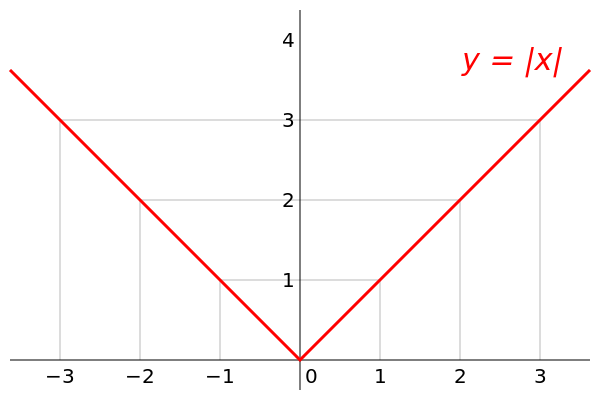
\includegraphics[height=5cm]{figures/Absolute_value_svg} 
\end{figure}


\noindent We hebben er toen ook op gewezen dat je voorzichtig moet
zijn met formules van het type $\sqrt{x^{2}}$.

\noindent Passen we dit toe op een functie die horizontaal verschoven
is: ${\displaystyle y=\sqrt{(x-1)^{2}}=\left|x-1\right|}$.

\noindent Als deze functie zou gegeven zijn als de veelterm ${\displaystyle x^{2}-2x+1}$,
dan loont het dus de moeite om dit te herschrijven als een volledig
kwadraat: ${\displaystyle x^{2}-2x+1=\left(x-1\right)^{2}}$.


\section{De signum functie}

De sign of signum functie $\textrm{sgn}(x)$ is een eenvoudige wiskundige
functie, die eigenlijk het teken van het argument aangeeft:

${\displaystyle \textrm{sgn}(x)=\begin{cases}
-1 & \textrm{als}\:x<0\\
0 & \textrm{\textrm{als}}\:x=0\\
+1 & \textrm{\textrm{als}}\:x>0
\end{cases}}$

\medskip{}


\noindent De grafiek van de signum functie:

\noindent 
\begin{figure}[h]
\centering{}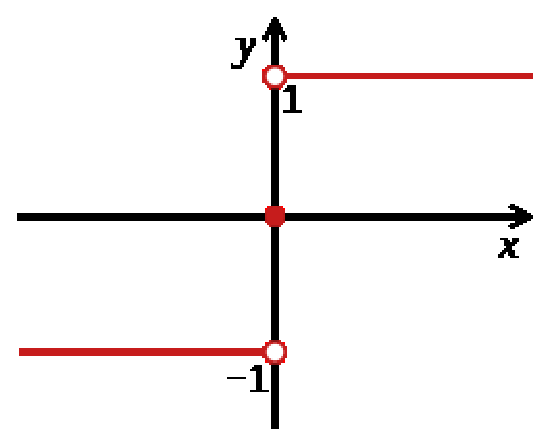
\includegraphics[height=5cm]{figures/Signum_function_svg} 
\end{figure}

\end{document}

%%\DeclareMathOperator{\tri}{tri} \DeclareMathOperator{\rect}{rect}
%\DeclareMathOperator{\sgn}{sgn} \DeclareMathOperator{\ramp}{ramp}
%\DeclareMathOperator{\sinc}{sinc}


\subsection{Verschuiven en herschalen}

%\begin{itemize}
%\item Wat gebeurt er met de grafiek van een functie als we bij het argument
%en/of bij de functie zelf, een getal optellen?
%\item Wat gebeurt er met de grafiek van een functie als we het argument
%en/of de functie zelf vermenigvuldigen met een getal?
%\end{itemize}

\subsubsection{Verschuiven}

Wanneer we de grafiek van $y=f(x)$ kennen, kunnen we met
verschuivingen (of translaties) de grafiek van $y=f(x+a)$ en $y=f(x)+a$
daaruit afleiden (met $a\in\mathbb{R}$).

De grafiek van $y=f(x+a)$ wordt verkregen uit de grafiek
van $y=f(x)$ door alle punten op de grafiek met een afstand van $a$
eenheden horizontaal te verschuiven (naar links als $a>0$, en naar
rechts als $a<0$).

Het lijkt misschien een beetje tegenstrijdig dat de grafiek
van een functie naar rechts verschuift als je bij het argument $x$
een negatief getal optelt. Maar kijk eens naar de sinus functie $f_{1}(x)=\sin(x)$
in onderstaand voorbeeld. We weten dat de sinus functie onder andere
een nulpunt heeft als het argument nul is, dus voor $x=0$. Als we
van $x$ de waarde $\frac{\pi}{2}$ aftrekken, dan bekomen we terug
datzelfde nulpunt als het argument nul is. Uit $x-\frac{\pi}{2}=0$
volgt dat dit het geval zal zijn als $x=+\frac{\pi}{2}$. Met andere
woorden, de functie $f_{2}(x)=\sin(x-\frac{\pi}{2})$ heeft dezelfde
grafiek als de functie $f_{1}(x)=\sin(x)$ maar is $\frac{\pi}{2}$
eenheden naar rechts verschoven.

%TODO figuur aanpassen
%\begin{figure}[h]
\begin{center}
	\input{2_elem_rekenvaardigheden_B/Fig_module_2_1_15_verschuiven_en_verschalen_1.tex}
\end{center}
%\end{figure}


\begin{center}
	\input{2_elem_rekenvaardigheden_B/Fig_module_2_1_15_verschuiven_en_verschalen_2}
\end{center}


%\begin{figure}[h]
%	\centering
%	\begin{subfigure}{.48\linewidth}
%	\includegraphics[height=5cm]{\string"2_elem_rekenvaardigheden_B/inputs/Verschuiven - horizontaal - naar links\string".eps}
%	\end{subfigure}
%	\begin{subfigure}{.48\linewidth}
%	 \includegraphics[height=5cm]{\string"2_elem_rekenvaardigheden_B/inputs/Verschuiven - horizontaal - naar rechts\string".eps} 
%	\end{subfigure}
%\end{figure}

De grafiek van $y=f(x)+a$ wordt verkregen uit de grafiek
van $y=f(x)$ door alle punten op de grafiek met een afstand van $a$
eenheden verticaal te verschuiven (naar beneden als $a<0$, en naar
boven als $a>0$).

%TODO figuur aanpassen
\begin{center}
	\input{2_elem_rekenvaardigheden_B/Fig_module_2_1_15_verschuiven_en_verschalen_3}
\end{center}


\begin{center}
	\input{2_elem_rekenvaardigheden_B/Fig_module_2_1_15_verschuiven_en_verschalen_4}
\end{center}



%\begin{figure}[h]
%	\centering
%	\begin{subfigure}{.48\linewidth}
%		\includegraphics[height=5cm]{\string"2_elem_rekenvaardigheden_B/inputs/Verschuiven - verticaal - naar omlaag\string".eps}
%	\end{subfigure}
%	\begin{subfigure}{.48\linewidth}
%		\includegraphics[height=5cm]{\string"2_elem_rekenvaardigheden_B/inputs/Verschuiven - verticaal - naar o%mhoog\string".eps}
%	\end{subfigure}
%\end{figure}

%%\begin{tabular}{ccc}
%%\includegraphics[height=5cm]{\string"2_elem_rekenvaardigheden_B/inputs/Verschuiven - verticaal - naar omlaag\string".eps}  &  & \includegraphics[height=5cm]{\string"2_elem_rekenvaardigheden_B/inputs/Verschuiven - verticaal -  naar omhoog\string".eps} \tabularnewline
%%\end{tabular}


\begin{voorbeeld}
hoe ziet de grafiek eruit van de functie $y=x^{2}+2x+3$?

We herschrijven de functie als: $y=\left(x^{2}+2x+1\right)+2=\left(x+1\right)^{2}+2$

We herkennen hierin de basisfunctie $y=x^{2}$. De gegeven functie
stelt dus een parabool voor die over 1 eenheid naar links en 2 eenheden
naar boven is verschoven.
\end{voorbeeld}


\subsubsection{Herschalen}

Wanneer we de grafiek van $y=f(x)$ kennen, kunnen we met
herschalen (of vermenigvuldigen) de grafiek van $y=f(ax)$ en $y=af(x)$
daaruit afleiden (met $a\in\mathbb{R}$).

De grafiek van $y=f(ax)$ wordt verkregen uit de grafiek
van $y=f(x)$ door, bij gelijkblijvende $y$-co\"ordinaten, alle $x$-co\"ordinaten
van de punten op de grafiek met een factor $\frac{1}{a}$ te vermenigvuldigen
(openrekken als $0<a<1$, en inkrimpen als $a>1$).

Voor $a=2$ bijvoorbeeld krimpt de grafiek in elkaar. Het
is alsof de functie dubbel zo snel verloopt.

%TODO figuur aanpassen
\begin{center}
	\input{2_elem_rekenvaardigheden_B/Fig_module_2_1_15_verschuiven_en_verschalen_5}
\end{center}

\begin{center}
	\input{2_elem_rekenvaardigheden_B/Fig_module_2_1_15_verschuiven_en_verschalen_6}
\end{center}




%\begin{figure}[h]
%\begin{subfigure}{.5\linewidth}
%\includegraphics[height=5cm]{\string"2_elem_rekenvaardigheden_B/inputs/Herschalen - horizontaal - openrekken\string".eps}
%\end{subfigure}
%\begin{subfigure}{.5\linewidth}
%\includegraphics[height=5cm]{\string"2_elem_rekenvaardigheden_B/inputs/Herschalen - horizontaal - inkrimpen\string".eps}
%\end{subfigure}	
%\end{figure}

Een bijzonder geval treedt op als $a=-1$: de grafiek van
$g(x)=f(-x)$ kan uit de grafiek van $f(x)$ worden verkregen door
van alle punten op de grafiek de $x$-co\"ordinaten met -1 te vermenigvuldigen,
dus door de grafiek van $f(x)$ te spiegelen ten opzichte van de $y$-as.
Op die manier kan je bijvoorbeeld heel eenvoudig afleiden dat de grafiek
van de functie $g(x)=\sqrt{-x}$ bestaat en het spiegelbeeld is van
$f(x)=\sqrt{x}$. Terwijl de functie $f(x)$ enkel gedefinieerd is
voor alle positieve re\"ele getallen, is de functie $g(x)$ dit enkel
voor alle negatieve re\"ele getallen.


De grafiek van $y=af(x)$ wordt verkregen uit de grafiek
van $y=f(x)$ door, bij gelijkblijvende $x$-co\"ordinaten, alle $y$-co\"ordinaten
van de punten op de grafiek met een factor $a$ te vermenigvuldigen
(inkrimpen als $0<a<1$, en openrekken als $a>1$).

%TODO figuur aanpassen
\begin{center}
	\input{2_elem_rekenvaardigheden_B/Fig_module_2_1_15_verschuiven_en_verschalen_7}
\end{center}

\begin{center}
	\input{2_elem_rekenvaardigheden_B/Fig_module_2_1_15_verschuiven_en_verschalen_8}
\end{center}




%\begin{figure}[h]
%	\begin{subfigure}{.5\linewidth}
%	\includegraphics[height=5cm]{\string"2_elem_rekenvaardigheden_B/inputs/Herschalen - verticaal - i%nkrimpen\string".eps}
%	\end{subfigure}
%	\begin{subfigure}{.5\linewidth}
%	\includegraphics[height=5cm]{\string"2_elem_rekenvaardigheden_B/inputs/Herschalen - verticaal - o%penrekken\string".eps}
%	\end{subfigure}	
%\end{figure}



%\DeclareMathOperator{\tri}{tri} \DeclareMathOperator{\rect}{rect}
%\DeclareMathOperator{\sgn}{sgn} \DeclareMathOperator{\ramp}{ramp}
%\DeclareMathOperator{\sinc}{sinc}


\subsection{Co\"ordinatenstelsels}

%\begin{itemize}
%\item Hoe kunnen we op een \'e\'enduidige manier elk punt in het vlak of de
%ruimte een plaats geven?
%\item Welke co\"ordinatenstelsels worden er vaak gebruikt?
%\end{itemize}
%Een co\"ordinatenstelsel is een wiskundige methode die wordt gebruikt
%om de ligging van een punt weer te geven.

\subsubsection{Cartesisch of rechthoekig co\"ordinatenstelsel}

De vergelijking $y=f(x)$ voegt aan iedere $x$-waarde \'e\'enduidig een
$y$-waarde toe. Met $x_{0}$ komt bijvoorbeeld $y_{0}$ overeen volgens
$y_{0}=f(x_{0})$. Het getallenpaar $(x_{0}\,,\,y_{0})$ kunnen we
als punt P in een rechthoekig of cartesisch co\"ordinatenstelsel tekenen.
De twee co\"ordinaat-assen staan loodrecht op elkaar, de horizontale
as noemen we de X-as en de verticale as de Y-as. Het snijpunt is de
oorsprong O.

\noindent Voor ieder getallenpaar krijgen we precies \'e\'en punt. De
verzameling van alle punten $(x\,,\,y=f(x))$ vormt de grafiek of
kromme van de functie. De grafiek laat het verloop van de functie
in een figuur zien.

\begin{figure}
\centering
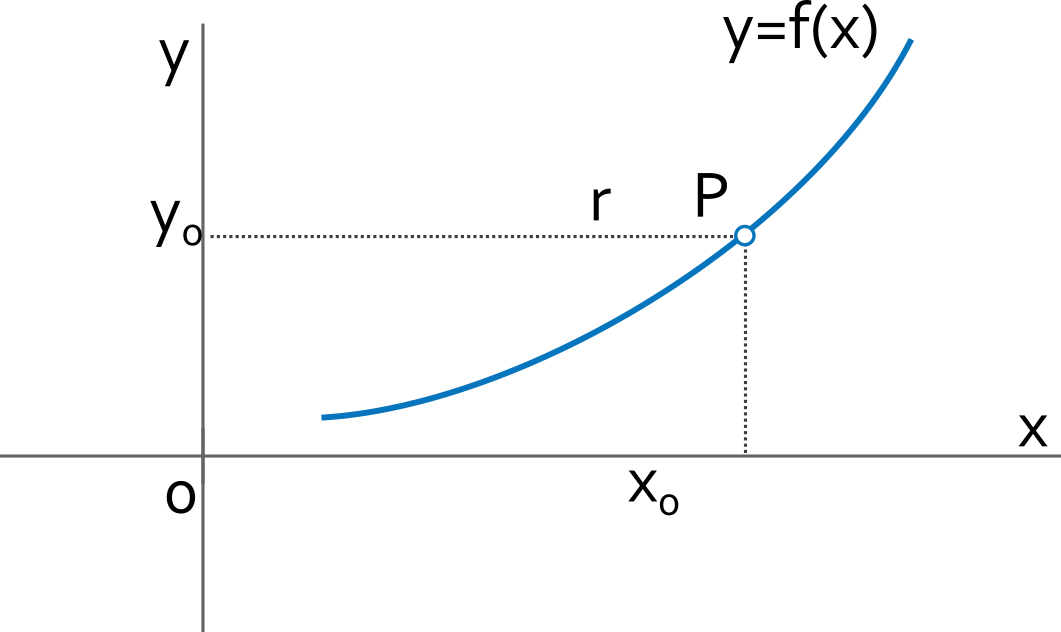
\includegraphics[height=5cm]{2_elem_rekenvaardigheden_B/inputs/figuur10}
\end{figure}

\begin{table}
	\centering
\begin{tabular}{|c|l|l|}
	\hline 
	We zeggen dat: & $x_{0},y_{0}$  & zijn de rechthoekige of cartesische co\"ordinaten\\
	\hline 
	& $x_{0}$  & is de abscis van het punt P\\
	\hline 
	& $y_{0}$ & is de ordinaat van het punt P\\
	\hline 
\end{tabular}
\end{table}


\noindent Het cartesisch co\"ordinatenstelsel is de gebruikelijke manier
om een punt in een vlak aan te duiden. Omdat in dit platte vlak twee
co\"ordinaten nodig zijn om een punt vast te leggen, zeggen we dat een
vlak tweedimensionaal is. In feite is 'de dimensie van een ruimte'
het aantal co\"ordinaten dat nodig is om de plaats van alle punten in
die ruimte precies te kunnen bepalen. Zo bestaat de klassieke 3D-ruimte
uit 3 dimensies en zijn er dus 3 co\"ordinaten $(x,y,z)$ nodig om de
plaats van elk punt \'e\'enduidig te beschrijven. 

\textbf{Parametervoorstelling van een functie}

\noindent Het is bij de wiskundige beschrijving van een bewegend lichaam
vaak handig om de positie van het lichaam weer te geven door cartesische
co\"ordinaten die zelf een functie van de tijd zijn. We noteren dan:
\[
x=x(t)\:,\;y=y(t)\quad\textrm{met}\:t_{1}\leq t\leq t_{2}
\]

\noindent We noemen een dergelijke voorstelling met een hulpvariabele
$t$ de parametervoorstelling van een functie. In de natuurwetenschappen
en de techniek betekent de parameter $t$ meestal de tijd of een hoek.

\noindent We krijgen voor iedere waarde van t uit het interval $t_{1}\leq t\leq t_{2}$
precies \'e\'en punt van de kromme.\medskip{}


\noindent Voorbeeld 1: de horizontale worp

\noindent een lichaam wordt van een bepaalde hoogte horizontaal met
een constante beginsnelheid $v_{0}$ weggeworpen. T.g.v. de zwaartekracht
verloopt de beweging vervolgens als een parabool (parabolische baan).
De parametervergelijkingen van deze beweging zijn:

\[
x=v_{0}t\:,\;y=\frac{1}{2}gt^{2}\quad\textrm{met}\:t\geq0
\]


\noindent Door het elimineren van de parameter vinden we de expliciete
vergelijking van de grafiek (parabool). Dit doen we door t uit de
vergelijking van $x$ te halen en te substitueren in de vergelijking
van $y$:

uit $x=v_{0}t$ volgt dat $t=\frac{x}{v_{0}}$ zodat $y=\frac{1}{2}gt^{2}=\frac{1}{2}g\left(\frac{x}{v_{0}}\right)^{2}=\frac{g}{2v_{0}^{2}}x$


\noindent Voorbeeld 2: de cirkel

Een veel gebruikte parametrisatie voor de cirkel met vergelijking
$x^{2}+y^{2}=R^{2}$ is de volgende:

\noindent 
\[
x=R\cos(t)\:,\;y=R\sin(t)\quad\textrm{met}\:0\leq t<2\pi
\]


Opmerkingen:
\begin{itemize}
\item de parameter $t$ stelt nu een hoek voor (uitgedrukt in radialen).
Omdat $t=0$ en $t=2\pi$ hetzelfde punt voorstellen, zal men meestal
$2\pi$ niet opnemen in het interval. Vandaar het $<$ en niet nog
eens het $\leq$-symbool.
\item om uit de parametervergelijkingen de cartesische vergelijking voor
de cirkel te bekomen moeten we de parameter t elimineren. Daarvoor
gebruiken we een trucje. We weten dat voor elke hoek $\alpha$ de
goniometrische grondformule geldt: $\cos^{2}\alpha+\sin^{2}\alpha=1$.
Substitueren we nu $\cos(t)=\frac{x}{R}$ en $\sin(t)=\frac{y}{R}$
in de grondformule dan bekomen we inderdaad $x^{2}+y^{2}=R^{2}$ .
\end{itemize}

\subsubsection{Poolco\"ordinaten}

De poolco\"ordinaten $\left(r,\theta\right)$ van een punt P in een
vlak zijn de afstandsco\"ordinaat $r$ en de hoekco\"ordinaat $\theta$.
We noemen de afstand $r$ de radius of de voerstraal en de hoek $\theta$
het argument.

\begin{figure}
\centering
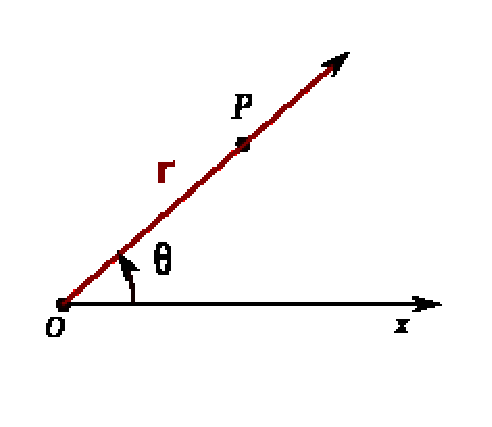
\includegraphics{2_elem_rekenvaardigheden_B/inputs/Poolcoordinaten_wikipedia}
\end{figure}

Enkele opmerkingen:
\begin{itemize}
\item we defini\"eren de voerstraal $r$ steeds positief, dus $r\geq0$.
\item we defini\"eren de hoek $\theta$ positief als de pijl van de positieve
X-as naar de plaatsvector van P tegen de klok in draait (andersom
is de hoek negatief). Een hoek $\theta$ is \'e\'enduidig bepaald op veelvouden
van 360\textdegree{} (of veelvouden van $2\pi$ in radialen) na. Meestal
wordt de hoek $\theta$ gegeven in het interval $0\text{\textdegree}\leq\theta\leq360\text{\textdegree}$
of $0\leq\theta\leq2\pi$. I.p.v. de Griekse letter theta ($\theta$
) wordt ook vaak de letter phi ( $\varphi$ ) als hoekaanduiding gebruikt.
\item de X- en Y-as maken geen deel uit van dit co\"ordinatenstelsel. We tekenen
echter wel vaak een horizontale en verticale hulplijn om het uitzetten
van de hoeken te vergemakkelijken.
\item het poolco\"ordinatenstelsel is een kromlijnig co\"ordinatenstelsel: de
co\"ordinaatlijnen zijn concentrische cirkels met de oorsprong O als
middelpunt en langs stralen die radiaal vanuit O lopen. We noemen
de oorsprong ook vaak 'de pool' en de X-as de 'poolas'.
\item de pool (dus de oorsprong O) heeft als voerstraal $r=0$ terwijl de
hoek $\theta$ onbepaald is.
\item poolco\"ordinaten worden ook gebruikt bij het voorstellen van en het
werken met complexe getallen.
\end{itemize}


\noindent Soms is het handig of noodzakelijk om over te stappen van
cartesische co\"ordinaten naar poolco\"ordinaten of omgekeerd. Daarvoor
gebruiken we het volgende stel transformatievergelijkingen:

\begin{minipage}{.48\linewidth}
%\begin{table}
	\begin{tabular}{|l|c|l|}
		\hline 
		cartesische co\"ordinaten &  & poolco\"ordinaten  \\
		\hline
		gegeven P met $\left(x,y\right)$ & $\rightarrow$ & dan is $\begin{cases}
		r=\sqrt{x^{2}+y^{2}}\\
		\textrm{tg}\theta=\frac{y}{x}
		\end{cases}$  \\
		dan is $\begin{cases}
		x=r.\cos\theta\\
		y=r.\sin\theta
		\end{cases}$ & $\leftarrow$ & gegeven P met $\left(r,\theta\right)$ \\
		\hline 
	\end{tabular}
%\end{table}
\end{minipage}
\hspace{1cm}
\begin{minipage}{.48\linewidth}
	\centering
	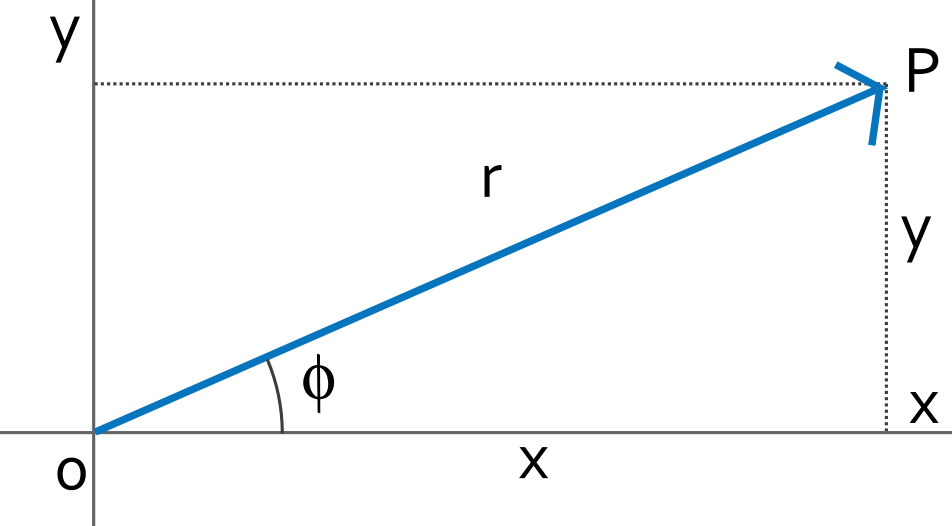
\includegraphics[width=0.7\linewidth]{2_elem_rekenvaardigheden_B/inputs/figuur9}
\end{minipage}


Opmerking: let op bij het berekenen van de hoek $\theta$. Je rekenmachine
zal als resultaat van de $\textrm{Arctg}\left(\frac{y}{x}\right)$
een hoek geven in het 1ste of 4de kwadrant. Je moet dus zelf, bij
het resultaat van je rekenmachine nog 180\textdegree{} of $\pi$ optellen
als het punt P in het 2de of 3de kwadrant ligt.

\noindent De voorstelling van een functie in poolco\"ordinaten

\noindent Een functie (kromme) in poolco\"ordinaten wordt beschreven
door een vergelijking van de vorm:
\[
r=r(\theta)
\]


\noindent We stellen een functiewaardentabel op voordat we de grafiek
van de functie tekenen. Voor verschillende waarden $\theta_{1}$ ,
$\theta_{2}$ , $\theta_{3}$ , ... berekenen we de bijhorende voerstralen
$r_{1}=r\left(\theta_{1}\right)$ , ... Daarna tekenen we de punten
met co\"ordinaten $\left(r_{1},\theta_{1}\right)$ , ... en verbinden
deze d.m.v. een vloeiende lijn.

\begin{minipage}{.48\linewidth}
	\centering
	\begin{tabular}{|c|c|}
		\hline 
		$\theta$ & $r=r(\theta)$\\
		\hline 
		\hline 
		$\theta_{1}$ & $r_{1}=r\left(\theta_{1}\right)$ \\
		\hline 
		$\theta_{2}$ & $r_{2}=r\left(\theta_{2}\right)$ \\
		\hline 
		$\vdots$ & $\vdots$\\
		\hline 
	\end{tabular}
\end{minipage}
\begin{minipage}{.48\linewidth}
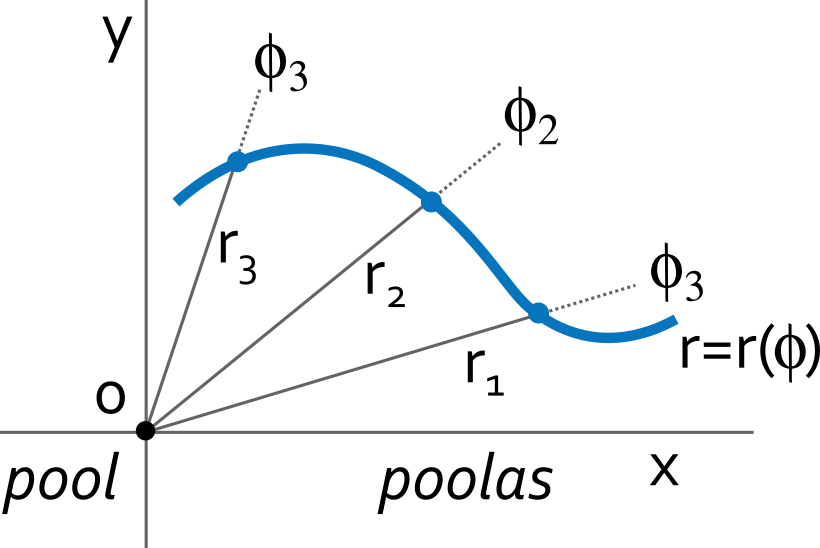
\includegraphics[height=5cm]{2_elem_rekenvaardigheden_B/inputs/figuur11}\\
In de figuur zijn de hoeken aangeduid met $\varphi$ ipv $\theta$
\end{minipage}



Voorbeeld 1: de spiraal van Archimedes

Schets de kromme met vergelijking $r=\theta$ waarbij $0\leq\theta\leq2\pi$

We stellen een functiewaardentabel op (tip: kies niet te veel, maar
ook niet te weinig hoeken; de intervallen tussen de hoeken hoeft niet
noodzakelijk overal even groot te zijn).

\begin{minipage}{.48\linewidth}
	\centering
	\begin{tabular}{|c|c|}
		\hline 
		$\theta$ & $r=r(\theta)=\theta$\\
		\hline 
		\hline 
		$0$ & 0\\
		\hline 
		$\frac{\pi}{4}$ & 0.785 \\
		\hline 
		$\frac{\pi}{2}$ & 1.571\\
		\hline 
		$3\frac{\pi}{4}$ & 2.356\\
		\hline 
		$\pi$ & 3.142\\
		\hline 
		$3\frac{\pi}{2}$ & 4.712\\
		\hline 
		$2\pi$ & 6.283\\
		\hline 
	\end{tabular}
\end{minipage}
\begin{minipage}{.48\linewidth}
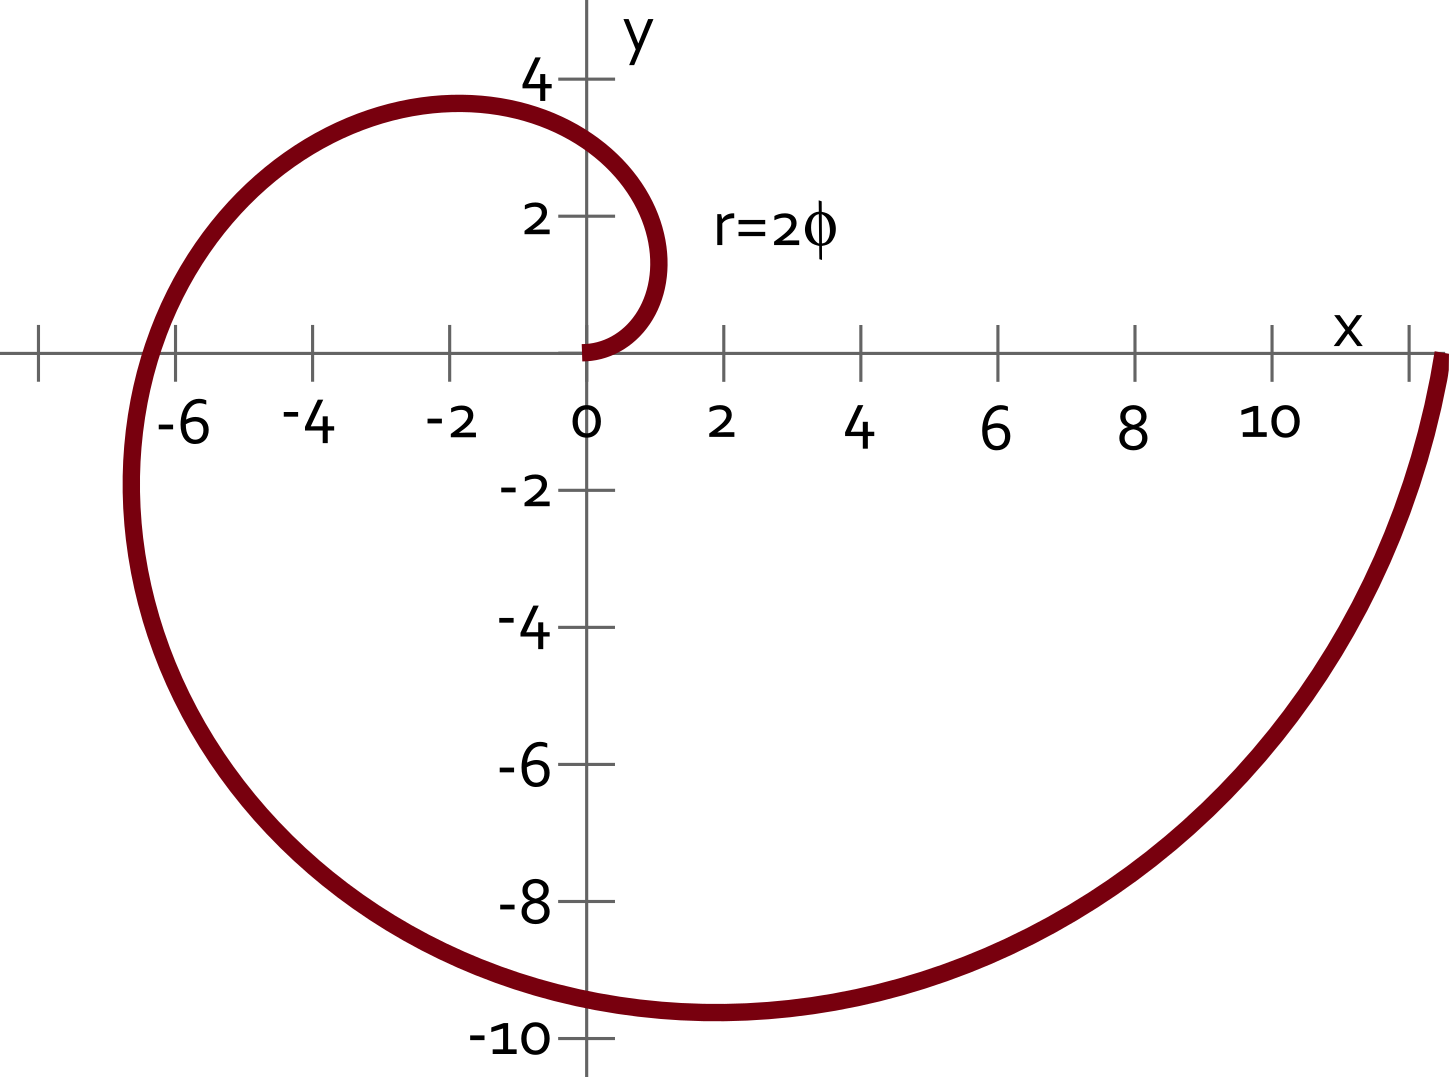
\includegraphics[height=5cm]{2_elem_rekenvaardigheden_B/inputs/figuur8}
\end{minipage}

Voorbeeld 2: de cardio\"ide

Schets de kromme met vergelijking $r=1+\cos\theta$ waarbij $0\text{\textdegree}\leq\theta\leq360\text{\textdegree}$

We stellen een functiewaardentabel op. Wegens de symmetrie t.o.v.
de X-as berekenen we slechts de radius-waarden tussen 0\textdegree{}
en 180\textdegree .

\begin{minipage}{0.5\linewidth}
	\centering
\begin{tabular}{|c|c|}
\hline 
$\theta$ & $r=r(\theta)$\\
\hline 
\hline 
0\textdegree{} & 2\\
\hline 
30\textdegree{} & 1.866\\
\hline 
60\textdegree{} & 1.5\\
\hline 
90\textdegree{} & 1\\
\hline 
120\textdegree{} & 0.5\\
\hline 
150\textdegree{} & 0.134\\
\hline 
180\textdegree{} & 0\\
\hline 
\end{tabular}
\end{minipage}
\begin{minipage}{.48\linewidth}
%	\begin{figure}
	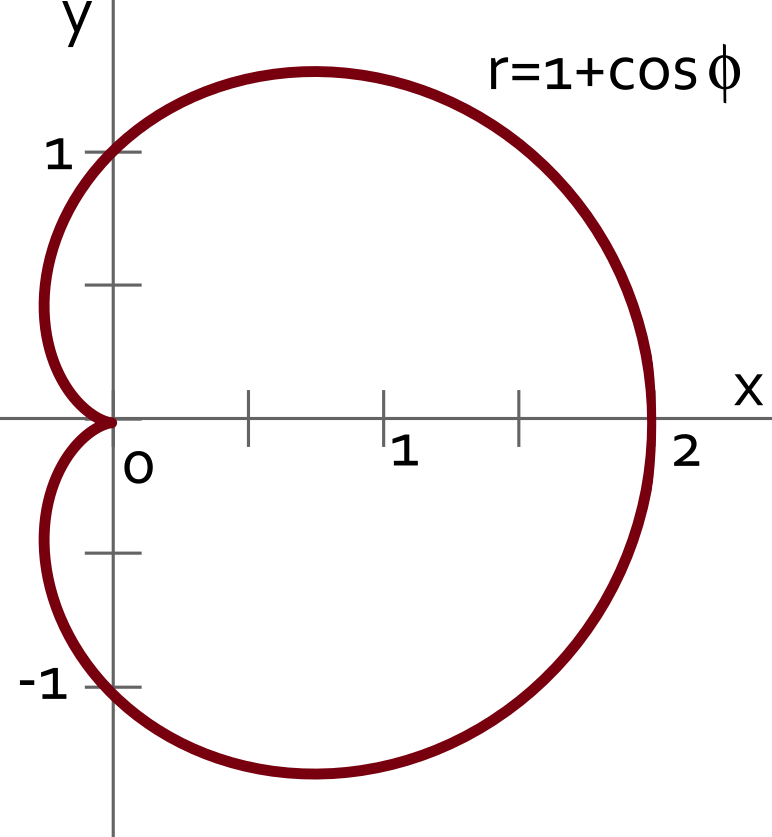
\includegraphics[height=5cm]{2_elem_rekenvaardigheden_B/inputs/figuur7.png}
%	\end{figure}
\end{minipage} 

Voorbeeld 3: de cirkel

Schets de kromme met vergelijking $r=2$ waarbij $0\text{\textdegree}\leq\theta<360\text{\textdegree}$

Bij elke hoek $\theta$ hoort dezelfde voerstraal, namelijk $r=2$.
Het heeft dus weinig zin om een functiewaardentabel op te stellen.

Opmerking: de cartesische vergelijking van een cirkel heeft een duidelijk
ingewikkeldere notatie: $x^{2}+y^{2}=2^{2}$. Schrijven we $y$ expliciet
dan zien we meteen ook dat dit eigenlijk geen functie is (met elke
$x$-waarde komen immers 2 $y$-waarden overeen): $y=\pm\sqrt{4-x^{2}}$



\section{Limieten}

\subsection{Het begrip limiet}

Bij het bestuderen van het gedrag van een functie stuiten we soms
op het probleem dat de functie in een bepaald punt niet gedefini\"eerd
is. Dit kan bijvoorbeeld optreden als het voorschrift van de functie
een breuk is waarvan de noemer nul wordt in dat punt. Toch willen
we vaak weten hoe de grafiek van die functie in de buurt van zo'n
punt er uitziet. Ook zijn we ge\"interesseerd in het gedrag van een
functie als het argument zeer groot of zeer sterk negatieve waarden
aanneemt.

Het begrip limiet is dus een belangrijke bouwsteen van de
analyse. De begrippen continu\"iteit, onbepaalde integraal en bepaalde
integraal steunen allen op het limietbegrip. Ook meetkundig is het
limietbegrip van belang: men heeft het nodig bij de definitie van
afgeleiden en asymptoten.


\subsubsection{De verzameling $\bar{\mathbb{R}}$}

Gegeven is de verzameling van de re\"ele getallen $\mathbb{R}$. Stel,
we nemen als deelverzameling het halfopen interval $[5,10[$ van $\mathbb{R}$.
Er bestaat dan bijvoorbeeld een getal uit die verzameling dat kleiner
of gelijk is aan alle elementen uit die deelverzameling. We noteren
dit als $\forall x\in[5,10[$ waarvoor geldt dat $x\ge5$. In dit
geval is het gezochte getal 5. Maar dit is niet altijd zo eenvoudig.




Nemen we de deelverzameling $\{...3,5,7,9\}$ van $\mathbb{R}$.
Welk getal kunnen we vinden dat kleiner is dan alle elementen uit
deze deelverzameling? Het getal 1? Of -1? Of -100? Het antwoord wordt
gevonden door de verzameling uit te breiden met de elementen plus
oneindig ($+\infty$) en min oneindig ($-\infty$).




We zeggen nu dat ``streep R streep'' gelijk is aan: $\overline{\mathbb{R}}=\mathbb{R}\cup\{\text{\textminus\ensuremath{\infty}},+\text{\ensuremath{\infty}}\}$
waarbij $\forall x\in\mathbb{R}$ geldt dat $\text{\textminus\ensuremath{\infty}}<x<+\text{\ensuremath{\infty}}$.




Merk op dat de elementen $\text{\textminus\ensuremath{\infty}}$
en $+\text{\ensuremath{\infty}}$ zelf geen re\"ele getallen zijn. Let
ook op met het symbool $\infty$: afhankelijk van de context kan dit
\textquotedblleft$+\infty$\textquotedblright betekenen, maar ook \textquotedblleft$+\infty\:\mathrm{of}\:\text{\textminus\ensuremath{\infty}}$\textquotedblright.
In dit laatste geval schrijven we soms $\pm\infty$.


\subsubsection{Rekenen met $\infty$}

Alhoewel $\text{\textminus\ensuremath{\infty}}$ en $+\text{\ensuremath{\infty}}$
geen re\"ele getallen zijn (maar wel symbolen), kunnen we er toch (mits
enige voorzichtigheid) mee rekenen.



\begin{tabel*}{}
	\centering
	\begin{tabular}{lcc|ll}
		\multicolumn{3}{c|}{vermenigvuldiging} & \multicolumn{2}{c}{optelling}\\
		\hline 
		$a\cdot (+\infty)=+\infty$ & als & $a>0$ & $\pm\infty+a=\pm\infty$ & met $a\in\mathbb{R}$\\
		$a\cdot (+\infty)=-\infty$ & als & $a<0$ &  & \\
		$a\cdot (-\infty)=-\infty$ & als & $a>0$ &  & \\
		$a\cdot (-\infty)=+\infty$ & als & $a<0$ &  & \\
		&  &  &  & \\
		$(+\infty)\cdot (+\infty)=+\infty$ &  &   & $(+\infty)+(+\infty)=+\infty$ & \\
		$(-\infty)\cdot (-\infty)=+\infty$ &  &   & $(-\infty)+(-\infty)=-\infty$ & \\
		$(+\infty)\cdot (-\infty)=-\infty$ &  &   &  & \\
	\end{tabular}
\end{tabel*}




$\frac{1}{\infty}=0$ maar let op: $\frac{1}{0}=\infty$
en dus onbepaald (want $\infty$ is geen re\"eel getal).

Soms maken we nog onderscheid tussen een heel klein positief
of heel klein negatief getal: $\frac{1}{0^{+}}=+\infty$ en $\frac{1}{0^{-}}=-\infty$




De volgende vormen zijn ook onbepaald: $\frac{0}{0}$ en
$\frac{\infty}{\infty}$ , $0\cdot \infty$, $+\infty-\infty$ , $0{}^{0}$
, $\infty{}^{0}$ , $1{}^{\infty}$.

Hoezo, $1{}^{\infty}$ is onbepaald? Dit is toch gewoon
$1\cdot 1\cdot 1\cdot 1\cdot \,\ldots$ en dus gelijk aan $1$!? Het antwoord hierop vind
je op het einde van dit hoofdstukje.

Merk op dat de vormen $\frac{0}{0}$ en $\frac{\infty}{\infty}$
infeite hetzelfde betekenen, immers $\frac{a}{b}$ kan je ook schrijven
als $\frac{\frac{1}{b}}{\frac{1}{a}}$.

\subsection{Intu\"itieve uitleg limieten}
\begin{minipage}{.25\linewidth}
	\raggedright
	
\includegraphics[width=4cm]{2_elem_rekenvaardigheden_B/inputs/QR_Code_LIMIETEN_module2new}
\end{minipage}
\begin{minipage}{.7\linewidth}
	Zie filmpje MOOC.
\end{minipage}

\subsection{Limieten en continu\"iteit}

\subsubsection{Het limietbegrip}

Als $x$ nadert tot $a$, dan nadert $f(x)$ tot $b$.

We zeggen wiskundig: de limiet van $f(x)$ voor $x$ gaande
naar $a$ is $b$.

We noteren dit als: $\lim_{x\to a}f(x)=b$

Grafisch:


\begin{figure}[H]
\centering
\tikzsetfigurename{Fig_module_2_2_1_limietbegripvb1}

\begin{center}
\begin{tikzpicture}[scale=0.7,cap=round]

% Styles
\tikzstyle{axes}=[]
\tikzstyle help lines=[color=blue!50,very thin,dotted]

% grid
\draw[style=help lines,step=1cm] (-0.9,-0.9) grid (6.9,8.9);

\draw[->] (-1,0) -- (7,0) node[right] {$x$};
\draw[->] (0,-1) -- (0,9) node[above] {$y$};

%\draw[fill,cyan](1,1)circle [radius=0.025];
%FUNCTIEVOORSCHRIFTEN



%\draw[teal,cap=rect,line width=1, opacity=1, domain=-2:2] plot (\x, {
%	pow(\x,2)  		% <- plaats het functievoorschrift hier
%}) node[right,opacity=1]{$h(x)=x^2$};

%\draw[red,cap=rect,line width=1, opacity=1, domain=-1.5:1.5] plot (\x, {
%	pow(\x,4)  		% <- plaats het functievoorschrift hier
%}) node[opacity=1,above,xshift=-3.5cm]{$p(x)=x^4$};

\draw[blue,cap=rect,line width=1, opacity=1, domain=3:6] plot (\x, {
	pow(\x-4,3)+1	% <- plaats het functievoorschrift hier
}) node[opacity=1,xshift=+1cm]{};

\draw[-,red] (0,3.3)--(5.3,3.3); 
\draw[-,red] (5.3,0)--(5.3,3.3); 

\draw[-,gray] (0,1.6)--(4.8,1.6); 
\draw[-,gray] (4.8,0)--(4.8,1.6); 

\draw[-,gray] (0,7.3)--(5.8,7.3); 
\draw[-,gray] (5.8,0)--(5.8,7.3); 


\draw[red] (5.3,3.3) circle[radius=0.1];

\draw[] (5.3,-0.2) node[below,red] {$a$};

\draw[] (-0.2,3.3) node[left,red] {$f(a)$};


\draw[] (4.8,1.6) circle[radius=0.1];



\draw[] (4.8,-0.2) node[below] {$x$};
\draw[] (-0.2,1.6) node[left] {$f(x)$};



\draw[] (5.8,7.3) circle[radius=0.1];

\draw[] (5.8,-0.2) node[below] {$x$};
\draw[] (-0.2,7.3) node[left] {$f(x)$};

%\draw[orange,cap=rect,line width=1, opacity=1, domain=-1.4:1.4] plot (\x, {
%	pow(\x,5)  		% <- plaats het functievoorschrift hier
%}) node[right,opacity=1]{$g(x)=x^5$};



%\draw[cyan,cap=rect,ultra thick, domain=1:2] plot (\x, {\x*\x-1}) node[above, right]{};
%\draw[red,cap=rect, loosely dashed, ultra thick, domain=-2:2] plot (\x, {(\x*\x-1)+0.05}) node[above,yshift=-.7cm, right]{};

%legende



%getallen op de x-as en lijntjes   
%\foreach \x/\xtext in {0,2,4,6}
%	\draw[xshift=\x cm] (0pt,1pt) -- (0pt,0pt) node[below,fill=white]
%	{$\xtext$}; 
	
%getallen op de y-as en lijntjes  
%BEGIN LUS
%\foreach \y/\ytext in {2,4,6,8}
%	\draw[yshift=\y cm] (1pt,0pt) -- (0pt,0pt) node[left,fill=white]
%	{$\ytext$}; %EINDE LUS



\end{tikzpicture}
\end{center}



\end{figure}


\begin{voorbeeld}
de functie is continu in $a$ 

$f(x)=x+1$


\begin{figure}[H]
	\centering
	\tikzsetfigurename{Fig_module_2_2_1_limietbegripvb1}
\begin{center}
\begin{tikzpicture}[scale=0.7,cap=round]

% Styles
\tikzstyle{axes}=[]
\tikzstyle help lines=[color=blue!50,very thin,dotted]

% grid
\draw[style=help lines,step=1cm] (-3.9,-1.9) grid (5.9,5.9);

\draw[->] (-4,0) -- (6,0) node[right] {$x$};
\draw[->] (0,-2) -- (0,6) node[above] {$y$};

%\draw[fill,cyan](1,1)circle [radius=0.025];
%FUNCTIEVOORSCHRIFTEN





%getallen op de x-as en lijntjes   
\foreach \x/\xtext in {-3,-2,-1,0,1,2,3,4,5}
\draw[xshift=\x cm] (0pt,1pt) -- (0pt,0pt) node[below,fill=white]
{$\xtext$};

%getallen op de y-as en lijntjes  
%BEGIN LUS
\foreach \y/\ytext in {-1,1,2,3,4,5}
\draw[yshift=\y cm] (1pt,0pt) -- (0pt,0pt) node[left,fill=white]
{$\ytext$}; %EINDE LUS


\draw[teal,cap=rect,line width=1, opacity=1, domain=-3:5] plot (\x, {
	\x+1  		% <- plaats het functievoorschrift hier
}) node[right,opacity=1]{$f(x)=x+1$};



%\draw[cyan,cap=rect,ultra thick, domain=1:2] plot (\x, {\x*\x-1}) node[above, right]{};
%\draw[red,cap=rect, loosely dashed, ultra thick, domain=-2:2] plot (\x, {(\x*\x-1)+0.05}) node[above,yshift=-.7cm, right]{};

%legende






\end{tikzpicture}
\end{center}


\end{figure}


We merken meteen op dat $dom\,f=\mathbb{R}$ (m.a.w. we mogen voor
$x$ elk re\"eel getal kiezen).

Als we $x$ voldoende dicht laten naderen tot bijvoorbeeld $1$, dan
nadert $f(x)$ tot $2$ (zie grafiek).

We noteren dit als: $\lim_{x\to1}f(x)=\lim_{x\to1}(x+1)=2$
en dit is hier ook $=f(1)$.

Omdat $\lim_{x\to1}(x+1)=f(1)$ zeggen we dat deze
functie \textbf{continu} is in het punt $x=1$.

\end{voorbeeld}


\begin{voorbeeld}
de functie is discontinu in $a$

$f(x)=\frac{2x\text{\texttwosuperior}-2x}{x-1}=\frac{2x(x-1)}{x-1}$

De noemer mag niet nul worden. Dus het domein van de functie is: $domf=\mathbb{R}\setminus\{1\}$

\begin{figure}[H]
	\centering
			\tikzsetfigurename{Fig_module_2_2_1_limietbegripvb2}
\begin{center}
	\begin{tikzpicture}[scale=0.7,cap=round]
	
	% Styles
	\tikzstyle{axes}=[]
	\tikzstyle help lines=[color=blue!50,very thin,dotted]
	
	% grid
	\draw[style=help lines,step=1cm] (-3.9,-1.9) grid (5.9,5.9);
	
	\draw[->] (-4,0) -- (6,0) node[right] {$x$};
	\draw[->] (0,-2) -- (0,6) node[above] {$y$};
	
	%\draw[fill,cyan](1,1)circle [radius=0.025];
	%FUNCTIEVOORSCHRIFTEN
	
	
	
	
	
	%getallen op de x-as en lijntjes   
	\foreach \x/\xtext in {-3,-2,-1,0,1,2,3,4,5}
	\draw[xshift=\x cm] (0pt,1pt) -- (0pt,0pt) node[below,fill=white]
	{$\xtext$};
	
	%getallen op de y-as en lijntjes  
	%BEGIN LUS
	\foreach \y/\ytext in {-1,1,2,3,4,5}
	\draw[yshift=\y cm] (1pt,0pt) -- (0pt,0pt) node[left,fill=white]
	{$\ytext$}; %EINDE LUS
	
	
	\draw[teal] (1,2) circle[radius=0.1] node[right]{$(1,2) $};
	
	\draw[teal,cap=rect,line width=1, opacity=1, domain=-1:0.99] plot (\x, {
		(	2*\x *(\x-1) ) / (	\x-1 ) 		% <- plaats het functievoorschrift hier
	}) node[right,opacity=1]{};
	
	
	\draw[teal,cap=rect,line width=1, opacity=1, domain=1.01:3] plot (\x, {
		(	2*\x *(\x-1) ) / (	\x-1 ) 		% <- plaats het functievoorschrift hier
	}) node[right,opacity=1]{$f(x)=\frac{2x(x-1)}{(x-1)}$};
	
	
	%\draw[cyan,cap=rect,ultra thick, domain=1:2] plot (\x, {\x*\x-1}) node[above, right]{};
	%\draw[red,cap=rect, loosely dashed, ultra thick, domain=-2:2] plot (\x, {(\x*\x-1)+0.05}) node[above,yshift=-.7cm, right]{};
	
	%legende
	
	
	
	
	
	
	\end{tikzpicture}
\end{center}


\end{figure}



Als we nu terug $x$ voldoende dicht laten naderen tot $1$, dan nadert
$f(x)$ terug tot $2$ (zie grafiek).

We noteren dit als: $\lim_{x\to1}f(x)= \lim_{x\to1}\frac{2x(x-1)}{x-1}=2$
maar dit is $\neq f(1)$ want 1 behoort niet tot het domein van deze
functie. En toch bestaat de limiet voor $x\rightarrow1$.

Hier is $\lim_{x\to1}\frac{2x(x-1)}{x-1}\neq f(1)$
. De limiet is dus niet gelijk aan de functiewaarde; we zeggen dat
de functie \textbf{niet-continu} of \textbf{discontinu} is in het
punt $x=1$.

\end{voorbeeld}

\subsubsection{Continu versus discontinu}

Een functie $f$ is continu in een \textbf{punt} $x=a$ als: $\lim_{x\to a}f(x)=f(a)$

Het is belangrijk dat je inziet dat voor de limietberekenaar
de functiewaarde niet belangrijk is, immers je gaat naar het punt
$a$ zonder het punt $a$ zelf ooit te bereiken. Dit is het principe
van het limietbegrip. Pas als je gaat kijken naar continu\"iteit moet
je ook rekening houden met (het al dan niet bestaan van) de functiewaarde.


Het is je waarschijnlijk al opgevallen dat we nog niks gezegd
hebben over ``hoe je naar het punt $a$ kan gaan''. Dit kan immers
langs de linkerkant van $a$, of langs de rechterkant van $a$ gebeuren
(we spreken van respectievelijk de linker- en de rechterlimiet).


\begin{notatie}
	We noteren: %
\begin{tabular}{l|l}
linkerlimiet & $\lim_{\overset{x\rightarrow a}{<}}f(x)$\\
rechterlimiet & $\lim_{\overset{x\rightarrow a}{>}}f(x)$\\
\end{tabular}
\end{notatie}

\begin{ftonthoud}
	Twee belangrijke besluiten:
\begin{itemize}
\item als de linkerlimiet en de rechterlimiet beiden bestaan en gelijk zijn
aan elkaar, dan bestaat \textbf{de} limiet $\lim_{x\to a}f(x)$
. De grafiek loopt van beide kanten naar dat punt $(a,f(a))$ toe.
\item als bovendien de limiet ook nog gelijk is aan $f(a)$ dan zit daar
geen discontinu\"iteit (geen gaatje), dus de grafiek bestaat in dat
punt. Dit betekent dat de limiet gelijk is aan de functiewaarde en
dat de functie continu is in het punt $a$.
\end{itemize}
Vereenvoudigd zegt men soms ook dat een functie continu
is als je de grafiek ervan kunt tekenen zonder je potlood van het
papier te halen.
\end{ftonthoud}


Tenslotte zeggen we dat een functie $f$ continu is over
het gesloten interval $[a,b]$ indien:
\begin{itemize}
\item $f$ rechts continu is in $a$ (m.a.w. $\lim_{\overset{x\rightarrow a}{>}}f(x)=f(a)$
)
\item $f$ links continu is in $b$ (m.a.w. $\lim_{\overset{x\rightarrow b}{<}}f(x)=f(b)$
)
\item $\forall x\in]a,b[$ geldt dat $f$ continu is in $x$ (m.a.w. $f(x)$
is continu in elk punt binnen het interval).
\end{itemize}



Je ziet dat een functie $f$ discontinu kan zijn in een
punt $a$ omdat:
\begin{itemize}
\item ze in dat punt niet gedefinieerd is: $f(a)$ bestaat niet
\item ze in dat punt een sprong maakt: $\lim_{\overset{x\rightarrow a}{<}}f(x)$$\neq\lim_{\overset{x\rightarrow a}{>}}f(x)$
\item haar definitie in dat punt niet overeenkomt met de limiet: $\lim_{x\to a}f(x)$$=b\neq f(a)$ 
\item haar waarde onbeperkt toeneemt naarmate men het punt nadert: $\lim_{x\to a}f(x)$$=\pm\infty$ 
\end{itemize}

\subsection{Voorbeelden}
%TODO
\begin{voorbeeld}
	\ \\


\begin{figure}[H]
	\centering
	\tikzsetfigurename{Fig_module_2_2_1_Continuvb1}

\begin{center}
	\begin{tikzpicture}[scale=0.7,cap=round]
	
	% Styles
	\tikzstyle{axes}=[]
	\tikzstyle help lines=[color=blue!50,very thin,dotted]
	
	% grid
	\draw[style=help lines,step=1cm] (-1.9,-1.9) grid (6.9,5.9);
	
	\draw[->] (-2,0) -- (7,0) node[right] {$x$};
	\draw[->] (0,-2) -- (0,6) node[above] {$y$};
	
	%\draw[fill,cyan](1,1)circle [radius=0.025];
	%FUNCTIEVOORSCHRIFTEN
	
	\draw[gray](3,0)--(3,2); 
	\draw[gray](0,2)--(3,2); 
	
	\draw[teal] (3,-0.7) node[below]{$a$};  
	\draw[teal] (-0.4,2) node[left]{$g(a)$};  

	
	%getallen op de x-as en lijntjes   
	\foreach \x/\xtext in {-1,0,1,2,3,4,5}
	\draw[xshift=\x cm] (0pt,1pt) -- (0pt,0pt) node[below,fill=white]
	{$\xtext$};
	
	%getallen op de y-as en lijntjes  
	%BEGIN LUS
	\foreach \y/\ytext in {-1,1,2,3,4,5}
	\draw[yshift=\y cm] (1pt,0pt) -- (0pt,0pt) node[left,fill=white]
	{$\ytext$}; %EINDE LUS
	
	
	\draw[teal] (3,2) circle[radius=0.1] node[right]{};
	
	\draw[teal,cap=rect,line width=1, opacity=1, domain=3:7,samples=500] plot (\x, {
		 2+pow((\x-3),0.5) 		% <- plaats het functievoorschrift hier
	}) node[xshift=-1cm,yshift=-1.2cm]{$g(x) = 2+ \sqrt{x-3}$};
	

	
	%\draw[cyan,cap=rect,ultra thick, domain=1:2] plot (\x, {\x*\x-1}) node[above, right]{};
	%\draw[red,cap=rect, loosely dashed, ultra thick, domain=-2:2] plot (\x, {(\x*\x-1)+0.05}) node[above,yshift=-.7cm, right]{};
	
	%legende
	
	
	
	
	
	
	\end{tikzpicture}
\end{center}



\end{figure}

	
Bestaan de limieten als $x=3$?

\begin{math}
\left. \begin{array}{l}
\lim_{\overset{x\rightarrow3}{<}}g(x) \text{ bestaat niet want dom} \ g=[3,+\infty[\\
 \lim_{\overset{x\rightarrow3}{>}}g(x)=2
\end{array}
\right\}
\Rightarrow \lim_{x\to3}g(x) \text{bestaat niet want } \lim_{\overset{x\rightarrow3}{<}}g(x) \neq \lim_{\overset{x\rightarrow3}{>}}g(x).
\end{math}

Is de functie continu in $x=3$?

\begin{math}
\centering
\left. \begin{array}{l}
g \text{ is niet linkscontinu in }3\\
g \text{ is rechtscontinu in }3
\end{array}
\right\}
\Rightarrow g \text{ is discontinu in }3.
\end{math}

\end{voorbeeld}
\begin{voorbeeld}
	\ \\


\begin{figure}[H]
	\centering
			\tikzsetfigurename{Fig_module_2_2_1_Continuvb2}


\begin{center}
	\begin{tikzpicture}[scale=0.7,cap=round]
	
	% Styles
	\tikzstyle{axes}=[]
	\tikzstyle help lines=[color=blue!50,very thin,dotted]
	
	% grid
	\draw[style=help lines,step=1cm] (-5.9,-0.9) grid (6.9,2.9);
	
	\draw[->] (-6,0) -- (7,0) node[right] {$x$};
	\draw[->] (0,-1) -- (0,3) node[above] {$y$};
	
	%\draw[fill,cyan](1,1)circle [radius=0.025];
	%FUNCTIEVOORSCHRIFTEN
	


	\draw[dashed](0,1)--(2,1); 
	
	\draw[teal] (-0.5,-1) node[left]{$f(a)$};  
	\draw[teal] (-0.5,1) node[left]{$f(a)$};  

	
	%getallen op de x-as en lijntjes   
	\foreach \x/\xtext in {-5,-4,-3,-2,-1,0,1,2,3,4,5}
	\draw[xshift=\x cm] (0pt,1pt) -- (0pt,0pt) node[below,fill=white]
	{$\xtext$};
	
	%getallen op de y-as en lijntjes  
	%BEGIN LUS
	\foreach \y/\ytext in {-1,1,2}
	\draw[yshift=\y cm] (1pt,0pt) -- (0pt,0pt) node[left,fill=white]
	{$\ytext$}; %EINDE LUS
	
	
	\draw[teal] (2,-1) circle[radius=0.1] node[right]{};
	\draw[teal] (2,1) circle[radius=0.1] node[right]{};
	
	\draw[teal,cap=rect,line width=1, opacity=1, domain=-5:2,samples=500] plot (\x, {
		 -1 		% <- plaats het functievoorschrift hier
	}) node[xshift=-1cm,yshift=-1.2cm]{$ $};
	
	\draw[teal,cap=rect,line width=1, opacity=1, domain=2:7,samples=500] plot (\x, {
	1 		% <- plaats het functievoorschrift hier
	}) node[xshift=-2cm,yshift=-2cm]{$f(x)= \frac{|x-2|}{x-2} $};


	
\draw[teal] (-0.5,-1) node[left]{$f(a)$};  
\draw[teal] (-0.5,1) node[left]{$f(a)$};  
	
	%\draw[cyan,cap=rect,ultra thick, domain=1:2] plot (\x, {\x*\x-1}) node[above, right]{};
	%\draw[red,cap=rect, loosely dashed, ultra thick, domain=-2:2] plot (\x, {(\x*\x-1)+0.05}) node[above,yshift=-.7cm, right]{};
	
	%legende
	
	
	
	
	
	
	\end{tikzpicture}
\end{center}



\end{figure}



Bestaan de limieten in $x=2$?

\begin{math}
\left. \begin{array}{l}
\lim_{\overset{x\rightarrow2}{<}}f(x)=-1 \\
 \lim_{\overset{x\rightarrow2}{>}}f(x)=+1
\end{array}
\right\}
\Rightarrow \lim_{x\to2}f(x) \text{bestaat niet want } \lim_{\overset{x\rightarrow2}{<}}f(x) = \lim_{\overset{x\rightarrow2}{>}}f(x).
\end{math}

Is de functie continu in $x=2$?

\begin{math}
\centering
\left. \begin{array}{l}
g \text{ is niet linkscontinu in }2\\
g \text{ is niet rechtscontinu in }2
\end{array}
\right\}
\Rightarrow f \text{ is discontinu in }2.
\end{math}


\end{voorbeeld}


\begin{voorbeeld}
	

\begin{figure}[H]
	\centering
	
		\tikzsetfigurename{Fig_module_2_2_1_Continuvb3}
\begin{center}
	\begin{tikzpicture}[scale=0.7,cap=round]
	
	% Styles
	\tikzstyle{axes}=[]
	\tikzstyle help lines=[color=blue!50,very thin,dotted]
	
	% grid
	\draw[style=help lines,step=1cm] (-3.9,-1.9) grid (5.9,7.9);
	
	\draw[->] (-4,0) -- (6,0) node[right] {$x$};
	\draw[->] (0,-2) -- (0,8) node[above] {$y$};
	
	%\draw[fill,cyan](1,1)circle [radius=0.025];
	%FUNCTIEVOORSCHRIFTEN
	
	
	\draw[dashed] (1,0)--(1,5);
		\draw[dashed] (0,5)--(1,5);
	
	
	%getallen op de x-as en lijntjes   
	\foreach \x/\xtext in {-3,-2,-1,0,1,2,3,4,5}
	\draw[xshift=\x cm] (0pt,1pt) -- (0pt,0pt) node[below,fill=white]
	{$\xtext$};
	
	%getallen op de y-as en lijntjes  
	%BEGIN LUS
	\foreach \y/\ytext in {-1,1,2,3,4,5,6,7}
	\draw[yshift=\y cm] (1pt,0pt) -- (0pt,0pt) node[left,fill=white]
	{$\ytext$}; %EINDE LUS
	
	
	\draw[teal] (1,5) circle[radius=0.1] node[right]{};
	
	\draw[teal,cap=rect,line width=1, opacity=1, domain=-0.5:0.99] plot (\x, {
		(5* \x*\x -5*\x   ) / ( \x-1   )% <- plaats het functievoorschrift hier
	}) node[right,opacity=1]{};
	
	
	\draw[teal,cap=rect,line width=1, opacity=1, domain=1.01:1.5] plot (\x, {
		(5* \x*\x -5*\x   ) / ( \x-1   ) 		% <- plaats het functievoorschrift hier
	}) node[right,opacity=1]{$f(x)=\frac{5x^2-5x}{x-1}$};
	
	
	%\draw[cyan,cap=rect,ultra thick, domain=1:2] plot (\x, {\x*\x-1}) node[above, right]{};
	%\draw[red,cap=rect, loosely dashed, ultra thick, domain=-2:2] plot (\x, {(\x*\x-1)+0.05}) node[above,yshift=-.7cm, right]{};
	
	%legende
	
	
	
	
	
	
	\end{tikzpicture}
\end{center}


\end{figure}


Bestaan de limieten in $x=1$?

\begin{math}
\left. \begin{array}{l}
\lim_{\overset{x\rightarrow1}{<}}f(x)=5 \\
 \lim_{\overset{x\rightarrow1}{>}}f(x)=5
\end{array}
\right\}
\Rightarrow \lim_{x\to1}f(x) \text{ bestaat en is } 5
\end{math}

Is de functie continu in $x=1$?

\begin{math}
\centering
\left. \begin{array}{l}
f \text{ is niet linkscontinu in }1\\
f \text{ is niet rechtscontinu in }1
\end{array}
\right\}
\Rightarrow f \text{ is discontinu in }1.
\end{math}


\end{voorbeeld}


\begin{voorbeeld}


\begin{figure}[H]
	\centering
	
		\tikzsetfigurename{Fig_module_2_2_1_Continuvb4}
\begin{center}
	\begin{tikzpicture}[scale=0.7,cap=round]
	
	% Styles
	\tikzstyle{axes}=[]
	\tikzstyle help lines=[color=blue!50,very thin,dotted]
	
	% grid
	\draw[style=help lines,step=1cm] (-3.9,-1.9) grid (5.9,7.9);
	
	\draw[->] (-4,0) -- (6,0) node[right] {$x$};
	\draw[->] (0,-2) -- (0,8) node[above] {$y$};
	
	%\draw[fill,cyan](1,1)circle [radius=0.025];
	%FUNCTIEVOORSCHRIFTEN
	
	

	\draw[dashed] (2,-1.5)--(2,7.5);
	
	
	%getallen op de x-as en lijntjes   
	\foreach \x/\xtext in {-3,-2,-1,0,1,2,3,4,5}
	\draw[xshift=\x cm] (0pt,1pt) -- (0pt,0pt) node[below,fill=white]
	{$\xtext$};
	
	%getallen op de y-as en lijntjes  
	%BEGIN LUS
	\foreach \y/\ytext in {-1,1,2,3,4,5,6,7}
	\draw[yshift=\y cm] (1pt,0pt) -- (0pt,0pt) node[left,fill=white]
	{$\ytext$}; %EINDE LUS
	
	
%	\draw[teal] (1,5) circle[radius=0.1] node[right]{};
	
	\draw[teal,cap=rect,line width=1, opacity=1, domain=-4:1.63] plot (\x, {
 pow(\x-2,-2 )% <- plaats het functievoorschrift hier
	}) node[right,opacity=1]{};
	
		\draw[teal,cap=rect,line width=1, opacity=1, domain=2.37:4] plot (\x, {
		pow(\x-2,-2 )% <- plaats het functievoorschrift hier
	}) node[right,opacity=1]{$f(x)=\frac{1}{(x-2)^2}$};
	
	%legende
	
	
	
	
	
	
	\end{tikzpicture}
\end{center}


\end{figure}



Bestaan de limieten in $x=2$?

\begin{math}
\left. \begin{array}{l}
\lim_{\overset{x\rightarrow2}{<}}f(x)=+\infty \\
 \lim_{\overset{x\rightarrow2}{>}}f(x)=+\infty
\end{array}
\right\}
\Rightarrow \lim_{x\to2}f(x)=+\infty.
\end{math}

Is de functie continu in $x=2$?

\begin{math}
\centering
\left. \begin{array}{l}
f \text{ is niet linkscontinu in }2\\
f \text{ is niet rechtscontinu in }2
\end{array}
\right\}
\Rightarrow f \text{ is discontinu in }2.
\end{math}

We merken nog op dat $\lim_{x\rightarrow+\infty}f(x)=0$ en $\lim_{x\rightarrow-\infty}f(x)=0$. Hier spreken we over een horizontale asymptoot met vergelijking $y=0$.

\end{voorbeeld}

\begin{voorbeeld}


\begin{figure}[H]
	\centering
			\tikzsetfigurename{Fig_module_2_2_1_Continuvb5}

\begin{center}
	\begin{tikzpicture}[scale=0.7,cap=round]
	
	% Styles
	\tikzstyle{axes}=[]
	\tikzstyle help lines=[color=blue!50,very thin,dotted]
	
	% grid
	\draw[style=help lines,step=1cm] (-3.9,-4.9) grid (8.9,7.9);
	
	\draw[->] (-4,0) -- (9,0) node[right] {$x$};
	\draw[->] (0,-5) -- (0,8) node[above] {$y$};
	
	%\draw[fill,cyan](1,1)circle [radius=0.025];
	%FUNCTIEVOORSCHRIFTEN
	
	
	
	\draw[dashed] (4,-5)--(4,7.5);
	
	
	%getallen op de x-as en lijntjes   
	\foreach \x/\xtext in {-3,-2,-1,0,1,2,3,4,5,6,7,8}
	\draw[xshift=\x cm] (0pt,1pt) -- (0pt,0pt) node[below,fill=white]
	{$\xtext$};
	
	%getallen op de y-as en lijntjes  
	%BEGIN LUS
	\foreach \y/\ytext in {-5,-4,-3,-2,-1,1,2,3,4,5,6,7}
	\draw[yshift=\y cm] (1pt,0pt) -- (0pt,0pt) node[left,fill=white]
	{$\ytext$}; %EINDE LUS
	
	
	%	\draw[teal] (1,5) circle[radius=0.1] node[right]{};
	
	\draw[teal,cap=rect,line width=1, opacity=1, domain=-4:3.5] plot (\x, {
		(\x-1)/(\x-4)% <- plaats het functievoorschrift hier
	}) node[right,opacity=1]{};
	
	\draw[teal,cap=rect,line width=1, opacity=1, domain=4.4:8] plot (\x, {
		(\x-1)/(\x-4)% <- plaats het functievoorschrift hier
	}) node[right,opacity=1]{$g(x)= \frac{ x-1}{x-4}$};
	
	%legende
	
	
	
	
	
	
	\end{tikzpicture}
\end{center}


\end{figure}



Bestaan de limieten in $x=4$?

\begin{math}
\left. \begin{array}{l}
\lim_{\overset{x\rightarrow4}{<}}g(x)=-\infty \\
 \lim_{\overset{x\rightarrow4}{>}}g(x)=+\infty
\end{array}
\right\}
\Rightarrow \lim_{x\to4}g(x) \text{ bestaat niet}.
\end{math}

Is de functie continu in $x=4$?

\begin{math}
\centering
\left. \begin{array}{l}
g \text{ is niet linkscontinu in }4\\
g \text{ is niet rechtscontinu in }4
\end{array}
\right\}
\Rightarrow f \text{ is discontinu in }4.
\end{math}

Er is een verticale asymptoot met vergelijking $x=4$.
Merk verder op dat $\lim_{x\rightarrow+\infty}g(x)=1$ en $\lim_{x\rightarrow-\infty}g(x)=1$.
Er is dus ook een horizontale asymptoot met vergelijking $y=1$.

\end{voorbeeld}

\subsection{Limieten - voorbeeld}


\begin{minipage}{.25\linewidth}
	\raggedright
	
\includegraphics[width=4cm]{2_elem_rekenvaardigheden_B/inputs/QR_Code_LIMIETENVOORBEELD_module2new}
\end{minipage}
\begin{minipage}{.7\linewidth}
	Zie filmpje MOOC.
\end{minipage}

\subsection{Limieten van functies (en asymptoten)}


\subsubsection{Limiet bij onbeperkte toename van het argument}

We stellen ons de vraag wat $f(x)$ wordt als we $x$ naar (plus of
min) oneindig laten gaan.

Laten we eerst naar een voorbeeld kijken. 
\begin{voorbeeld}
Stel $f(x)= 1-\frac{1}{x\text{\texttwosuperior}}$

\begin{figure}[H]
	\centering
 
		\tikzsetfigurename{Fig_module_2_2_1_AsymptootHorizontaal}


\begin{center}
	\begin{tikzpicture}[scale=0.7,cap=round]
	
	% Styles
	\tikzstyle{axes}=[]
	\tikzstyle help lines=[color=blue!50,very thin,dotted]
	
	% grid
	\draw[style=help lines,step=1cm] (-8.9,-4.9) grid (8.9,2.9);
	
	\draw[->] (-9,0) -- (9,0) node[right] {$x$};
	\draw[->] (0,-5) -- (0,3) node[above] {$y$};
	
	%\draw[fill,cyan](1,1)circle [radius=0.025];
	%FUNCTIEVOORSCHRIFTEN
	
	
	
	\draw[dashed] (-8,1)--(8,1);
	
	
	%getallen op de x-as en lijntjes   
	\foreach \x/\xtext in {-8,-7,-6,-5,-4,-3,-2,-1,0,1,2,3,4,5,6,7,8}
	\draw[xshift=\x cm] (0pt,1pt) -- (0pt,0pt) node[below,fill=white]
	{$\xtext$};
	
	%getallen op de y-as en lijntjes  
	%BEGIN LUS
	\foreach \y/\ytext in {-5,-4,-3,-2,-1,1,2}
	\draw[yshift=\y cm] (1pt,0pt) -- (0pt,0pt) node[left,fill=white]
	{$\ytext$}; %EINDE LUS
	
	
	%	\draw[teal] (1,5) circle[radius=0.1] node[right]{};
	

	
	\draw[teal,cap=rect,line width=1, opacity=1, domain=-9:-0.4,samples=500] plot (\x, {
		1- pow(\x*\x,-1 )% <- plaats het functievoorschrift hier
	}) node[right,opacity=1]{};

		\draw[teal,cap=rect,line width=1, opacity=1, domain=0.4:9,samples=500] plot (\x, {
		1- pow(\x*\x,-1 )% <- plaats het functievoorschrift hier
	}) node[right,opacity=1]{$f(x)= 1- \frac{1}{x^2}$};
	
	
	
	
	
	\end{tikzpicture}
\end{center}


\end{figure}


We stellen vast dat naarmate $x$ toeneemt, $f(x)$ waarden
aanneemt die onbeperkt dicht bij 1 komen te liggen. Hetzelfde gebeurt
wanneer $x$ negatief is, maar in absolute waarde onbeperkt toeneemt.
We kunnen dit noteren (en berekenen) a.d.h.v. de limietnotatie: $\lim_{x\to+\infty}\left(1-\frac{1}{x\text{\texttwosuperior}}\right)=1$
en $\lim_{x\to-\infty}\left(1-\frac{1}{x\text{\texttwosuperior}}\right)=1$
\end{voorbeeld}

Algemeen:

De afstand tussen de waarden van $f(x)$ en $b$ wordt willekeurig
klein, als het argument $x$ maar voldoende groot wordt (argument
neemt onbeperkt toe of af).


\begin{eqnarray*}
 \lim_{x\to+\infty}f(x)=b & \Leftrightarrow & \forall\varepsilon>0,\:\exists m>0:\:x>m\:\Rightarrow\left|f(x)-b\right|<\varepsilon\\
 \lim_{x\to-\infty}f(x)=b & \Leftrightarrow & \forall\varepsilon>0,\:\exists m>0:\:x<-m\:\Rightarrow\left|f(x)-b\right|<\varepsilon
\end{eqnarray*}

Dit houdt in dat men eerst een willekeurig positief getal $\varepsilon$
kiest en in functie van deze gekozen $\varepsilon$, vastlegt hoe
groot dan $m$ moet zijn. Dit is uitvoerbaar, hoe klein men $\varepsilon$
ook kiest. We kunnen ook zeggen: je kan $f(x)$ oneindig dicht bij
$b$ laten komen, mits je maar een heel grote waarde voor $x$ kiest.

De horizontale rechte met vergelijking $y=b$ noemen we de \textbf{horizontale
asymptoot} van de functie $f(x)$. In ons voorbeeld met de functie
$f(x)= 1-\frac{1}{x\text{\texttwosuperior}}$ is er
\'e\'en horizontale asymptoot met als vergelijking $y=1$. Merk op dat
de functie $f(x)$ deze horizontale rechte (de asymptoot) zowel voor
$x\rightarrow-\infty$ als voor $x\rightarrow+\infty$ langs de onderkant
benadert.

Het is ook mogelijk dat de waarden van $f(x)$ onbeperkt
toenemen, naarmate $x$ toeneemt, denk maar aan de veeltermfunctie
$f(x)=x\text{\texttwosuperior}+1$ of de exponenti\"ele functie $f(x)=3^{x}$.

We stellen vast dat naarmate $x$ toeneemt, ook $f(x)$
onbeperkt toeneemt: $ \lim_{x\to+\infty}3^{x}=+\infty$. 

Merk op dat de limiet van de functie $3^{x}$ voor $x$
gaande naar $\text{\textminus\ensuremath{\infty}}$ gewoon naar $0$
gaat. Dus de rechte met vergelijking $y=0$ is hier dan een horizontale
asymptoot.


\begin{figure}[H]
	\centering
			\tikzsetfigurename{Fig_module_2_2_1_AsymptootOneindig}
\begin{center}
	\begin{tikzpicture}[scale=0.7,cap=round]
	
	% Styles
	\tikzstyle{axes}=[]
	\tikzstyle help lines=[color=blue!50,very thin,dotted]
	
	% grid
	\draw[style=help lines,step=1cm] (-7.9,-0.9) grid (8.9,7.9);
	
	\draw[->] (-9,0) -- (9,0) node[right] {$x$};
	\draw[->] (0,-2) -- (0,8) node[above] {$y$};
	
	%\draw[fill,cyan](1,1)circle [radius=0.025];
	%FUNCTIEVOORSCHRIFTEN
	
	
	
%	\draw[dashed] (4,-5)--(4,7.5);
	
	
	%getallen op de x-as en lijntjes   
	\foreach \x/\xtext in {-8,-7,-6,-5,-4,-3,-2,-1,0,1,2,3,4,5,6,7,8}
	\draw[xshift=\x cm] (0pt,1pt) -- (0pt,0pt) node[below,fill=white]
	{$\xtext$};
	
	%getallen op de y-as en lijntjes  
	%BEGIN LUS
	\foreach \y/\ytext in {-1,1,2,3,4,5,6,7}
	\draw[yshift=\y cm] (1pt,0pt) -- (0pt,0pt) node[left,fill=white]
	{$\ytext$}; %EINDE LUS
	
	
 \draw[teal] (0,1) circle[radius=0.1] node[right]{$(0,1)$};
	

	
	\draw[teal,cap=rect,line width=1, opacity=1, domain=-9:2] plot (\x, {
		pow(3,\x)% <- plaats het functievoorschrift hier
	}) node[right,opacity=1]{$f(x)=3^x$};
	
	%legende
	
	
	
	
	
	
	\end{tikzpicture}
\end{center}


\end{figure}

Algemeen:

De waarden van $f(x)$ worden groter dan om het even welk (groot)
re\"eel getal, als men $x$ maar voldoende groot neemt (argument neemt
onbeperkt toe of af).

\begin{eqnarray*}
 \lim_{x\to+\infty}f(x)=+\infty & \Leftrightarrow & \forall n>0,\:\exists m>0:\:x>m\:\Rightarrow f(x)>n\\
 \lim_{x\to+\infty}f(x)=-\infty & \Leftrightarrow & \forall n>0,\:\exists m>0:\:x>m\:\Rightarrow f(x)<-n\\
\end{eqnarray*} 

Hierbij legt men eerst vast hoe groot men wil dat $f(x)$ wordt; dit
is het getal $n$. In functie van die gekozen $n$ bepaalt men de
benodigde $m$ .

(gelijkaardige redenering en formuleringen voor $x\rightarrow\text{\textminus\ensuremath{\infty}}$).


\subsubsection{Limiet van een functie wanneer het argument onbeperkt nadert tot
een vaste waarde $a$}

Laten we nu even kijken naar het geval waarbij we $x$ naar een welbepaalde
vaste waarde $a$ laten gaan: ${\displaystyle \lim_{x\to a}}f(x)=b$.
We kunnen alvast zeggen dat $b\in\overline{\mathbb{R}}$.

\begin{voorbeeld}
	Als voorbeeld beschouwen we de functie $f(x)={\displaystyle \frac{5x\text{\texttwosuperior}-5x}{x-1}}={\displaystyle \frac{5x(x-1)}{x-1}}$ 


\begin{figure}[H]
\centering

		\tikzsetfigurename{Fig_module_2_2_1_Continuvb3}
\begin{center}
	\begin{tikzpicture}[scale=0.7,cap=round]
	
	% Styles
	\tikzstyle{axes}=[]
	\tikzstyle help lines=[color=blue!50,very thin,dotted]
	
	% grid
	\draw[style=help lines,step=1cm] (-3.9,-1.9) grid (5.9,7.9);
	
	\draw[->] (-4,0) -- (6,0) node[right] {$x$};
	\draw[->] (0,-2) -- (0,8) node[above] {$y$};
	
	%\draw[fill,cyan](1,1)circle [radius=0.025];
	%FUNCTIEVOORSCHRIFTEN
	
	
	\draw[dashed] (1,0)--(1,5);
		\draw[dashed] (0,5)--(1,5);
	
	
	%getallen op de x-as en lijntjes   
	\foreach \x/\xtext in {-3,-2,-1,0,1,2,3,4,5}
	\draw[xshift=\x cm] (0pt,1pt) -- (0pt,0pt) node[below,fill=white]
	{$\xtext$};
	
	%getallen op de y-as en lijntjes  
	%BEGIN LUS
	\foreach \y/\ytext in {-1,1,2,3,4,5,6,7}
	\draw[yshift=\y cm] (1pt,0pt) -- (0pt,0pt) node[left,fill=white]
	{$\ytext$}; %EINDE LUS
	
	
	\draw[teal] (1,5) circle[radius=0.1] node[right]{};
	
	\draw[teal,cap=rect,line width=1, opacity=1, domain=-0.5:0.99] plot (\x, {
		(5* \x*\x -5*\x   ) / ( \x-1   )% <- plaats het functievoorschrift hier
	}) node[right,opacity=1]{};
	
	
	\draw[teal,cap=rect,line width=1, opacity=1, domain=1.01:1.5] plot (\x, {
		(5* \x*\x -5*\x   ) / ( \x-1   ) 		% <- plaats het functievoorschrift hier
	}) node[right,opacity=1]{$f(x)=\frac{5x^2-5x}{x-1}$};
	
	
	%\draw[cyan,cap=rect,ultra thick, domain=1:2] plot (\x, {\x*\x-1}) node[above, right]{};
	%\draw[red,cap=rect, loosely dashed, ultra thick, domain=-2:2] plot (\x, {(\x*\x-1)+0.05}) node[above,yshift=-.7cm, right]{};
	
	%legende
	
	
	
	
	
	
	\end{tikzpicture}
\end{center}


\end{figure}


Wanneer we het argument $x$ laten naderen tot 1, dan stellen
we vast dat $f(x)$ nadert naar 5, en dit zowel langs de linker als
langs de rechterkant van 1.

We schrijven: ${\displaystyle \lim_{\overset{x\rightarrow1}{<}}}{\displaystyle \frac{5x\text{\texttwosuperior}-5x}{x-1}}=5$
en ${\displaystyle \lim_{\overset{x\rightarrow1}{>}}}{\displaystyle \frac{5x\text{\texttwosuperior}-5x}{x-1}}=5$ 

\end{voorbeeld}

Algemeen:

De afstand tussen de waarden $f(x)$ en $b$ wordt willekeurig klein,
als het argument $x$ maar dicht genoeg nabij $a$ komt.

\begin{eqnarray*}
{\displaystyle \lim_{\overset{x\rightarrow a}{<}}}f(x)=b & \Leftrightarrow & \forall\varepsilon>0,\:\exists\delta>0:\:x\in]a-\delta,a[\:\Rightarrow\left|f(x)-b\right|<\varepsilon\\
{\displaystyle \lim_{\overset{x\rightarrow a}{>}}}f(x)=b & \Leftrightarrow & \forall\varepsilon>0,\:\exists\delta>0:\:x\in]a,a+\delta[\:\Rightarrow\left|f(x)-b\right|<\varepsilon\\
\end{eqnarray*}

Hierbij gaat men ervan uit dat men eerst $\varepsilon$ vrij (willekeurig
klein) gekozen heeft en dat men dan $\delta$ bepaalt in functie van
de gekozen $\varepsilon$ .

Het gebruik van deze definitie veronderstelt dat $f(x)$ gedefinieerd
is in een omgeving van $a$ , maar niet noodzakelijk in $a$ zelf
(herinner je dat de limietberekenaar niet ge\"interesseerd is in $f(a)$
)! 

Even terzijde: aangezien in bovenstaand voorbeeld zowel
de linker- als rechterlimiet bestaan en gelijk zijn, bestaat de limiet:
${\displaystyle \lim_{x\to1}}{\displaystyle \frac{5x\text{\texttwosuperior}-5x}{x-1}}=5$.
Maar aangezien deze niet gelijk is aan de functiewaarde $f(1)$, want
$1\notin dom\,f$, kunnen we besluiten dat de functie discontinu is
in het punt $x=1$. Er zit bijgevolg een perforatie (gaatje) in de
grafiek van $f$. Maar we zouden dit \textquoteleft gat\textquoteright \ in het domein kunnen opheffen
door de functiewaarde in $x=1$ \textquoteleft erbij te defini\"eren\textquoteright: we stellen
de functiewaarde gelijk aan de limiet (zodat de nieuwe, uitgebreide
functie nu wel overal gedefinieerd is, en bovendien overal continu
is). We spreken dan van een ophefbare discontinu\"iteit.

De ``nieuwe'' functie $f(x)$ wordt nu gedefinieerd als:
$f(x):\:\begin{cases}
x\rightarrow\frac{5x\text{\texttwosuperior}-5x}{x-1} & \quad\mathrm{als}\:x\neq1\\
x\rightarrow5 & \quad\mathrm{als}\:x=1
\end{cases}$

Uiteraard is het ook mogelijk dat $f(x)$ onbeperkt toeneemt
als $x$ onbeperkt nadert tot $a$. 

\begin{voorbeeld}
Als voorbeeld bekijken we de functie
$f(x)=\frac{1}{x}$.


\begin{figure}[H]
	\centering
			\tikzsetfigurename{Fig_module_2_2_1_AsymptootVerticaal}

\begin{center}
	\begin{tikzpicture}[scale=0.7,cap=round]
	
	% Styles
	\tikzstyle{axes}=[]
	\tikzstyle help lines=[color=blue!50,very thin,dotted]
	
	% grid
	\draw[style=help lines,step=1cm] (-8.9,-4.9) grid (8.9,4.9);
	
	\draw[->] (-9,0) -- (9,0) node[right] {$x$};
	\draw[->] (0,-5) -- (0,5) node[above] {$y$};
	
	%\draw[fill,cyan](1,1)circle [radius=0.025];
	%FUNCTIEVOORSCHRIFTEN
	
	
	
%	\draw[dashed] (-8,1)--(8,1);
	
	
	%getallen op de x-as en lijntjes   
	\foreach \x/\xtext in {-8,-7,-6,-5,-4,-3,-2,-1,0,1,2,3,4,5,6,7,8}
	\draw[xshift=\x cm] (0pt,1pt) -- (0pt,0pt) node[below,fill=white]
	{$\xtext$};
	
	%getallen op de y-as en lijntjes  
	%BEGIN LUS
	\foreach \y/\ytext in {-5,-4,-3,-2,-1,1,2,3,4,5}
	\draw[yshift=\y cm] (1pt,0pt) -- (0pt,0pt) node[left,fill=white]
	{$\ytext$}; %EINDE LUS
	
	
	%	\draw[teal] (1,5) circle[radius=0.1] node[right]{};
	

	
	\draw[teal,cap=rect,line width=1, opacity=1, domain=-9:-0.2 ,samples=500] plot (\x, {
		 pow(\x,-1 )% <- plaats het functievoorschrift hier
	}) node[right,opacity=1]{};

	\draw[teal,cap=rect,line width=1, opacity=1, domain=0.2:9 ,samples=500] plot (\x, {
		pow(\x,-1 )% <- plaats het functievoorschrift hier
	}) node[right,opacity=1]{$f(x)= \frac{1}{x}$};
	
	
	
	
	
	\end{tikzpicture}
\end{center}


\end{figure}

Nadert $x$ langs rechts naar $0$, dit wil zeggen langs
waarden die groter zijn dan nul, dan worden de functiewaarden onbegrensd
groot in positieve zin. $f(x)$ nadert naar plus oneindig als $x$
langs rechts naar $0$ nadert. 

Nadert $x$ langs links naar $0$, dit wil zeggen langs
waarden die kleiner zijn dan nul, dan worden de functiewaarden onbegrensd
groot in negatieve zin. $f(x)$ nadert naar min oneindig als $x$
langs links naar $0$ nadert.


We schrijven: ${\displaystyle \lim_{\overset{x\rightarrow0}{>}}}{\displaystyle \frac{1}{x}}={\displaystyle \frac{1}{0^{+}}}=+\infty$
en ${\displaystyle \lim_{\overset{x\rightarrow0}{<}}}{\displaystyle \frac{1}{x}}={\displaystyle \frac{1}{0^{-}}}=-\infty$

\end{voorbeeld}
Algemeen:

Indien de waarden van $f(x)$ onbeperkt toenemen als $x$ maar dicht
genoeg bij $a$ komt, zegt men:

\begin{eqnarray*}
{\displaystyle \lim_{x\to a}}f(x)=+\infty & \Leftrightarrow & \forall n>0,\:\exists\delta>0:\:0<\left|x-a\right|<\delta\:\Rightarrow f(x)>n\\
{\displaystyle \lim_{x\to a}}f(x)=-\infty & \Leftrightarrow & \forall n>0,\:\exists\delta>0:\:0<\left|x-a\right|<\delta\:\Rightarrow f(x)<-n\\
\end{eqnarray*}

Hierbij gaat men ervan uit dat men eerst $n$ vrij gekozen heeft en
dat men dan $\delta$ bepaalt in functie van de gekozen $n$ .

De verticale rechte met vergelijking $x=a$ noemen we de \textbf{verticale
asymptoot} van de functie $f(x)$. In ons voorbeeld met de functie
$f(x)={\displaystyle \frac{1}{x}}$ is er \'e\'en verticale asymptoot
met als vergelijking $x=0$. Merk op dat de functie $f(x)$ deze verticale
rechte (de asymptoot) voor $x\rightarrow0^{-}$ naar $-\infty$ nadert,
en voor $x\rightarrow0^{+}$ naar $+\infty$ benadert.

\subsection{Epsilon delta definitie voor limieten}
\begin{minipage}{.25\linewidth}
	\raggedright
	
\includegraphics[width=4cm]{2_elem_rekenvaardigheden_B/inputs/QR_Code_EPSILONDELTA_module2new}
\end{minipage}
\begin{minipage}{.7\linewidth}
	Zie filmpje MOOC.
\end{minipage}

\subsection{Linkerlimiet en rechterlimiet}

Soms is de waarde van $\lim_{x\to a}f(x)$ afhankelijk
van de manier waarop we naar $a$ naderen. We maken in dat geval een
onderscheid tussen


\begin{center}
	\begin{tabular}{lcl}
	\multirow{2}{*}{de linkerlimiet} & $\lim_{\overset{x\rightarrow a}{<}}f(x)$ & we naderen $a$ langs de te kleine kant van $a$ ($\lyxmathsym{\textquotedblleft}<\lyxmathsym{\textquotedblright}$)\\
	& $\lim_{x\uparrow a}f(x)$ & $x$ stijgt tot aan de waarde van $a$\\
	\multirow{2}{*}{de rechterlimiet} & $\lim_{\overset{x\rightarrow a}{>}}f(x)$ & we naderen $a$ langs de te grote kant van $a$ $(\lyxmathsym{\textquotedblleft}>\lyxmathsym{\textquotedblright}$)\\
	& $\lim_{x\downarrow a}f(x)$ & $x$ daalt tot aan de waarde van $a$\\
\end{tabular}
\end{center}

Wanneer de linker- en rechterlimiet van elkaar verschillen,
zeggen we dat de limiet niet bestaat. 

Enkel als $\lim_{\overset{x\rightarrow a}{<}}f(x)=\lim_{\overset{x\rightarrow a}{>}}f(x)=\lim_{x\to a}f(x)=b\;(\in\mathbb{R})$
zeggen we dat \textbf{de} limiet bestaat.

Zie ook het paragraafje over \emph{continu versus discontinu}.

Redenen om een onderscheid te maken tussen een linker- en
een rechterlimiet kunnen zijn:
\begin{itemize}
\item dat $f(x)$ slechts aan \'e\'en van beide kanten van $a$ bestaat
\item dat naarmate $x$ nadert tot $a$, de waarden die $f(x)$ doorloopt
naar een ander waarde toe leiden naargelang $x$ kleiner of groter
blijft dan $a$ (sprongdiscontinu\"iteit).
\end{itemize}

\begin{voorbeeld}
	
Stel de functie $g(x)=\sqrt{x-4}$



\begin{figure}[H]
	\centering
			\tikzsetfigurename{Fig_module_2_2_1_Linkerlimiet_en_rechterlimiet}




\begin{center}
	\begin{tikzpicture}[scale=0.7,cap=round]
	
	% Styles
	\tikzstyle{axes}=[]
	\tikzstyle help lines=[color=blue!50,very thin,dotted]
	
	% grid
	\draw[style=help lines,step=1cm] (-1.9,-1.9) grid (8.9,2.9);
	
	\draw[->] (-2,0) -- (9,0) node[right] {$x$};
	\draw[->] (0,-2) -- (0,3) node[above] {$y$};
	
	%\draw[fill,cyan](1,1)circle [radius=0.025];
	%FUNCTIEVOORSCHRIFTEN
	
%	\draw[gray](3,0)--(3,2); 
%	\draw[gray](0,2)--(3,2); 
	
%	\draw[teal] (3,-0.7) node[below]{$a$};  
%	\draw[teal] (-0.4,2) node[left]{$g(a)$};  

	
	%getallen op de x-as en lijntjes   
	\foreach \x/\xtext in {-1,0,1,2,3,4,5,6,7,8}
	\draw[xshift=\x cm] (0pt,1pt) -- (0pt,0pt) node[below,fill=white]
	{$\xtext$};
	
	%getallen op de y-as en lijntjes  
	%BEGIN LUS
	\foreach \y/\ytext in {-1,1,2}
	\draw[yshift=\y cm] (1pt,0pt) -- (0pt,0pt) node[left,fill=white]
	{$\ytext$}; %EINDE LUS
	
	
	%\draw[teal] (3,2) circle[radius=0.1] node[right]{};
	
	\draw[teal,cap=rect,line width=1, opacity=1, domain=4:9,samples=500] plot (\x, {
		 pow((\x-4),0.5) 		% <- plaats het functievoorschrift hier
	}) node[xshift=-2cm,yshift=0cm]{$g(x) = \sqrt{x-4}$};
	

	
	%\draw[cyan,cap=rect,ultra thick, domain=1:2] plot (\x, {\x*\x-1}) node[above, right]{};
	%\draw[red,cap=rect, loosely dashed, ultra thick, domain=-2:2] plot (\x, {(\x*\x-1)+0.05}) node[above,yshift=-.7cm, right]{};
	
	%legende
	
	
	
	
	
	
	\end{tikzpicture}
\end{center}



\end{figure}

Deze functie bestaat enkel voor $x\geq4$ (we schrijven $dom\,g=[4,+\infty[$
)

We berekenen de linkerlimiet: $\lim_{\overset{x\rightarrow4}{<}}\sqrt{x-4}$
maar deze bestaat niet.

We berekenen de rechterlimiet: $\lim_{\overset{x\rightarrow4}{>}}\sqrt{x-4}=0$ 

We kunnen besluiten dat de limiet $\lim_{x\to4}\sqrt{x-4}$
niet bestaat (enkel de rechterlimiet bestaat wel).

\end{voorbeeld}

\subsection{Rekenregels}

In de onderstelling dat de limieten bestaan en eindig zijn gelden
de onderstaande rekenregels.

De limieten van $f(x)$ en $g(x)$ bestaan en zijn eindig,
dus: $\lim_{x\to a}f(x)=F$ en $\lim_{x\to a}g(x)=G$.

\begin{ftrekenregel}
	\ 
	\begin{tabel*}{}
	\centering
	\begin{tabular}{ll}

		1 & $\lim_{x\to a}c=c$ met $c$ een constante ($c\in\mathbb{R}$)\\

		2 & $\lim_{x\to a}x=a$  \\

		3 & $\lim_{x\to a}c\cdot f(x)=c\cdot \lim_{x\to a}f(x)=c\cdot F$  met $c\in\mathbb{R}$\\

		4 & $\lim_{x\to a}\left[f(x)\pm g(x)\right]=\lim_{x\to a}f(x)\pm\lim_{x\to a}g(x)=F\pm G$  \\

		5 & $\lim_{x\to a}\left[f(x)\cdot g(x)\right]=\lim_{x\to a}f(x)\cdot \lim_{x\to a}g(x)=F\cdot G$  \\

		6 & $\lim_{x\to a}\left[\frac{f(x)}{g(x)}\right]=\frac{\lim_{x\to a}f(x)}{\lim_{x\to a}g(x)}=\frac{F}{G}$  mits $\lim_{x\to a}g(x)\neq0$\\

		7 & $\lim_{x\to a}\left[f\left(g(x)\right)\right]=f\left(\lim_{x\to a}g(x)\right)$  mits $f$ continu is in het punt $\lim_{x\to a}g(x)=b$ \\


	\end{tabular}
\end{tabel*}
\end{ftrekenregel}

Eigenschap 7 in woorden: het omwisselen van het nemen van
de limiet en het nemen van de functiewaarde door de functie $f$ is
enkel toegestaan als $f$ een continue functie is in het betreffende
punt. We zeggen ook wel eens \textquoteleft de limiet passeert de functie $f$\textquoteright.

\textbf{Tip1}: de rekenregels voor $\infty$ zijn vrij eenvoudig
te onthouden en te gebruiken als $(+)\infty$ gelezen wordt als \textquoteleft een
heel groot (positief) getal\textquoteright, $-\infty$ als 'een heel groot negatief
getal', $0^{+}$ als \textquoteleft een heel klein positief getal\textquoteright en tenslotte $0^{-}$
als \textquoteleft een heel klein negatief getal\textquoteright.

\textbf{Tip2}: lees bijvoorbeeld de rekenregels 4, 5 en 6 ook eens
op een andere manier: ``de limiet van een som, is de som van de limieten''
...

\begin{voorbeeld}
\begin{eqnarray*}
\lim_{x\to+\infty}\frac{x}{4}&=&\frac{1}{4} \lim_{x\to+\infty}x=\frac{1}{4}\cdot (+\infty)=+\infty\\
\lim_{x\to3}\left[(x-2)(x+1)\right]&=& \lim_{x\to3}(x-2)\cdot  \lim_{x\to3}(x+1)=1\cdot 4=4\\
\lim_{x\to3}(x\text{\texttwosuperior}-x-2)&=& \lim_{x\to3}x\text{\texttwosuperior}- \lim_{x\to3}x-2\cdot  \lim_{x\to3}1=9-3-2=4\\
\lim_{\overset{x\rightarrow0}{>}}\left(2x-\frac{1}{x}\right)&=& \lim_{\overset{x\rightarrow0}{>}}2x- \lim_{\overset{x\rightarrow0}{>}}\frac{1}{x}=2\cdot 0-\left(+\infty\right)=-\infty\\
\lim_{x\to a}\left[\cos\left(g(x)\right)\right]&=&\cos\left( \lim_{x\to a}g(x)\right)\\
\lim_{x\to a}\left[e^{f(x)}\right]&=&e^{\lim_{x\to a}f(x)}
\end{eqnarray*}
\end{voorbeeld}

\subsection{Berekenen van limieten}

\subsubsection{Veeltermfuncties}

Een veeltermfunctie van n\textsuperscript{de} graad:

\begin{equation*}
f(x)=a_{n}x^{n}+a_{n-1}x^{n-1}+\ldots+a_{2}x^{2}+a_{1}x+a_{0}\text{ met }
a_{n}\in\mathbb{R}_{0}\text{ en }a_{n-1},\ldots,a_{0}\in\mathbb{R}
\end{equation*}

Elke veeltermfunctie is continu over $\mathbb{R}$ (want
het domein is immers $\mathbb{R}$).

De limiet voor $x$ gaande naar $a\in\overline{\mathbb{R}}$
van een veeltermfunctie is gelijk aan de functiewaarde (m.a.w. vervang
overal $x$ door $a$):

\begin{equation*}
\lim_{x\to a}\left(a_{n}x^{n}+a_{n-1}x^{n-1}+\ldots+a_{2}x^{2}+a_{1}x+a_{0}\right)=f(a)
\end{equation*}

Een speciaal geval is de limiet voor $x$ gaande naar oneindig.
In dit geval is het infeite enkel de hoogste graad term die van belang
is. Kijk maar:

\begin{eqnarray*}
\lim_{x\to+\infty}\left(a_{n}x^{n}+a_{n-1}x^{n-1}+\ldots+a_{1}x+a_{0}\right)&=& \lim_{x\to+\infty}a_{n}x^{n}\left(1+\frac{a_{n-1}x^{n-1}}{a_{n}x^{n}}+\ldots+\frac{a_{1}x}{a_{n}x^{n}}+\frac{a_{0}}{a_{n}x^{n}}\right) \\
&=& \lim_{x\to+\infty}a_{n}x^{n}(1+0+\ldots+0)\\
&=& \lim_{x\to+\infty}a_{n}x^{n}
\end{eqnarray*}


\begin{voorbeeld}
\begin{eqnarray*}
\lim_{x\to+\infty}\left(-x\text{\textthreesuperior}+6x+14\right)&=& \lim_{x\to+\infty}x\text{\textthreesuperior}\left(-1+\frac{6x}{x\text{\textthreesuperior}}+\frac{14}{x\text{\textthreesuperior}}\right)\\
&=& \lim_{x\to+\infty}x\text{\textthreesuperior}\left(-1\right)\\
&=&-\infty\\
& & \\
\lim_{x\to-\infty}\left(3x\text{\texttwosuperior}-4x+2\right)&=& \lim_{x\to-\infty}3x\text{\texttwosuperior}\left(1-\frac{4x}{3x\text{\texttwosuperior}}+\frac{2}{3x\text{\texttwosuperior}}\right)\\
&=&\lim_{x\to-\infty}3x\text{\texttwosuperior}\\
&=&+\infty
\end{eqnarray*}
\end{voorbeeld}

\subsubsection{Goniometrische en cyclometrische functies}

Laat ons meteen opmerken dat bij de berekeningen van deze limieten
het argument van de goniometrische of cyclometrische functie moet
uitgedrukt zijn in radialen. 

Enkele van deze limieten geven in eerste instantie aanleiding
tot de onbepaalde vorm $\frac{0}{0}$, maar toch kan men de limiet
vinden. We bekijken als voorbeeld de limiet van $ \lim_{x\to0}\frac{\sin x}{x}$.
Maken we een tabel met $x$-waarden die steeds dichter naar $0$ naderen,
dan zien we dat de verhouding $\frac{\sin x}{x}$ naar 1 gaat.

\begin{tabel*}{}
	\centering
	\begin{tabular}{l|l}
		$x$ & $\frac{\sin x}{x}$\\
		\hline 
		1 & 0,84147098480\\
		0,1 & 0,99833416646\\
		0,01 & 0,99998333341\\
		0,001 & 0,99999983333\\
		0,0001 & 0,99999999999\\
	\end{tabular}
\end{tabel*}


Aangezien $\lim_{\overset{x\rightarrow0}{<}}\frac{\sin x}{x}=\lim_{\overset{x\rightarrow0}{>}}\frac{\sin x}{x}=1$
kunnen we concluderen dat $\lim_{x\rightarrow0}\frac{\sin x}{x}=1$
(hetzelfde geldt trouwens ook voor $\lim_{x\rightarrow0}\frac{x}{\sin x}=1$
).


De limiet $\lim_{x\rightarrow\infty}\frac{\sin x}{x}=0$
kunnen we dan weer wiskundig bewijzen a.d.h.v. de zogenaamde insluitstelling.
Het komt er hierbij op neer dat je probeert een functie in te sluiten
tussen twee andere functies die beide een gelijke limiet $L$ hebben.
De limiet van de ingesloten functie is dan ook gelijk aan $L$.

We weten dat de sinus-functie altijd een waarde oplevert
tussen -1 en +1: $-1\leq\sin x\leq+1$.

Dit blijft gelden als we de vergelijking delen door een
positieve $x$ waarde: $\frac{-1}{x}\leq\frac{\sin x}{x}\leq\frac{+1}{x}$.

We weten ook dat: $\lim_{x\to\infty}\left(\frac{-1}{x}\right)=0$
en $\lim_{x\to\infty}\left(\frac{1}{x}\right)=0$.

Passen we nu de insluitstelling toe dan concluderen we dat
$\lim_{x\rightarrow\infty}\frac{\sin x}{x}=0$.


De limiet $\lim_{x\rightarrow0}\frac{\sin x}{x}=1$
noemen we een \textquoteleft standaardlimiet\textquoteright, en we kunnen hiermee een andere standaardlimiet
afleiden:

\begin{eqnarray*}
\lim_{x\rightarrow0}\frac{\tan x}{x}&=&\lim_{x\rightarrow0}\frac{\frac{\sin x}{\cos x}}{x}\\
&=&\lim_{x\rightarrow0}\frac{\sin x}{x\cdot \cos x}\\
&=&\lim_{x\rightarrow0}\frac{\sin x}{x}\cdot \lim_{x\rightarrow0}\frac{1}{\cos x}\\
&=&1\cdot \frac{1}{1}=1
\end{eqnarray*}


\begin{voorbeeld}

\begin{equation*}
\lim_{x\rightarrow0}\frac{\tan2x}{\sin3x}=\lim_{x\rightarrow0}\frac{\tan2x}{\sin3x}\cdot \frac{2x}{2x}\cdot \frac{3x}{3x}=\lim_{x\rightarrow0}\frac{\tan2x}{2x}\cdot \frac{2}{3}\cdot \frac{3x}{\sin3x}=\frac{2}{3}
\end{equation*}

\end{voorbeeld}



Nog enkele veel voorkomende limieten van goniometrische
en cyclometrische functies (tip: kijk ook eens naar hun grafiek of
de goniometrische cirkel)

\begin{table}[ht]
	\centering
	\begin{tabular}{c|c|c}
		$\lim_{\overset{x\rightarrow\frac{\pi}{2}}{<}}\tan x=+\infty$ & $\lim_{x\rightarrow+\infty}\arctan x=\frac{\pi}{2}$ & $\lim_{\overset{x\rightarrow1}{<}}\arcsin x=\frac{\pi}{2}$\\
		$\lim_{\overset{x\rightarrow-\frac{\pi}{2}}{>}}\tan x=-\infty$ & $\lim_{x\rightarrow-\infty}\arctan x=-\frac{\pi}{2}$ & $\lim_{\overset{x\rightarrow-1}{>}}\arcsin x=-\frac{\pi}{2}$\\
		$\lim_{\overset{x\rightarrow0}{<}}\cot x=-\infty$ & $\lim_{x\rightarrow+\infty}\mathrm{arccot}x=0$ & $\lim_{\overset{x\rightarrow1}{<}}\arccos x=0$\\s
		$\lim_{\overset{x\rightarrow0}{>}}\cot x=+\infty$  & $\lim_{x\rightarrow-\infty}\mathrm{arccot}x=\pi$ & $\lim_{\overset{x\rightarrow-1}{>}}\arccos x=\pi$\\
	\end{tabular}
\end{table}


\begin{figure}[H]
	\centering
			\tikzsetfigurename{Fig_module_2_1_13_Arctangent_Arccotangent}

\begin{tikzpicture}
\begin{axis}[ylabel=$y$,xlabel=$x$,
axis lines=middle,
xmin=-5.1,xmax = 5.1,ymin=-2,ymax=4,
%minor x tick num = 0.5,
xtick={-4,-3,-2,-1,0,1,2,3,4},
domain=-5:5,
xticklabel={},
ytick={-pi,-pi/2,0,pi/2,pi}, 
yticklabel={\textcolor{white}\ticknum}
]
\addplot[samples=500,color=red,thick] {rad(atan(x))};
\addplot[samples=500,color=blue,thick] {rad(90-atan(x))};



\draw[dotted] (-4,-2)--(-4,4);
\draw[dotted] (-3,-2)--(-3,4);
\draw[dotted] (-2,-2)--(-2,4);
\draw[dotted] (-1,-2)--(-1,4);

\draw[dotted] (1,-2)--(1,4);
\draw[dotted] (2,-2)--(2,4);
\draw[dotted] (3,-2)--(3,4);
\draw[dotted] (4,-2)--(4,4);



\draw[dotted] (-5,-pi/2)--(5,-pi/2);
\draw[dotted] (-5,pi/2)--(5,pi/2);
\draw[dotted] (-5,pi)--(5,pi);


\draw[](-0.6,-pi/2) node[left,above]{$-\pi/2$}; 
\draw[](-0.6,pi/2) node[left,above]{$\pi/2$}; 
\draw[](-0.2,pi) node[left,above]{$\pi$}; 

\draw[](-3.5,pi-0.2) node[left,below,blue]{$\text{Arccot}(x)$}; 
\draw[](3.5,pi/2+0.4) node[left,below,red]{$\text{Arctan}(x)$}; 


\end{axis}
\end{tikzpicture}
\end{figure}

\begin{figure}[H]
\centering
		\tikzsetfigurename{Fig_module_2_1_13_Arcsine_Arccosine}

\begin{tikzpicture}
\begin{axis}[ylabel=$y$,xlabel=$x$,
axis lines=middle,
xmin=-1.1,xmax = 1.1,ymin=-350,ymax=350,
%minor x tick num = 0.5,
xtick={-1,-0.5,0,0.5,1},
domain=-1:1,
xticklabel={},
ytick={-300,-250,-200,-150,-100,-50,0,50,100,150,200,250,300}, 
yticklabel={\textcolor{white}\ticknum}
]
\addplot[samples=500,color=red,thick] {asin(x)};
\addplot[samples=500,color=blue,thick] {acos(x)};

%\addplot[samples=500,color=red,thick] {asin(-x)+200};
%\addplot[samples=500,color=red,thick] {asin(-x)-200};
\draw[dotted] (-1,100)--(1,100);
\draw[dotted] (-1,200)--(1,200);
\draw[dotted] (-1,300)--(1,300);

\draw[dotted] (-1,-100)--(1,-100);
\draw[dotted] (-1,-200)--(1,-200);
\draw[dotted] (-1,-300)--(1,-300);


\draw[](-0.2,-100) node[]{$-\pi/2$}; 
\draw[](-0.2,-200) node[]{$-\pi$}; 

\draw[](-0.2,100) node[]{$\pi/2$}; 

\draw[](0.5,100) node[right,red]{$\text{arsin}(x) $}; 


\draw[](-0.2,200) node[]{$\pi$}; 

\draw[](-0.5,200) node[left,blue]{$\text{arccos}(x) $}; 


\draw[dotted] (0.5,-300)--(0.5,300);
\draw[dotted] (-0.5,-300)--(-0.5,300);

\draw[dotted] (1,-300)--(1,300);
\draw[dotted] (-1,-300)--(-1,300);

\end{axis}
\end{tikzpicture}
\end{figure}



\subsubsection{Exponenti\"ele en logaritmische functies}

Deze limieten laten zich gemakkelijk afleiden uit de grafieken:

Exponenti\"ele functies



\begin{figure}[H]
	\centering
	\tikzsetfigurename{Fig_module_2_2_1_expagroter1}
\begin{center}
	\begin{tikzpicture}[scale=0.7,cap=round]
	
	% Styles
	\tikzstyle{axes}=[]
	\tikzstyle help lines=[color=blue!50,very thin,dotted]
	
	% grid
	\draw[style=help lines,step=1cm] (-7.9,-0.9) grid (8.9,4.9);
	
	\draw[->] (-9,0) -- (9,0) node[right] {$x$};
	\draw[->] (0,-1) -- (0,5) node[above] {$y$};
	
	\draw[fill,cyan](0,1)circle [radius=0.025];
		\draw[] (0,1) node[right] {$(0,1)$};
	%FUNCTIEVOORSCHRIFTEN
	
	
	
%	\draw[dashed] (-8,1)--(8,1);
	
	
	%getallen op de x-as en lijntjes   
	\foreach \x/\xtext in {-8,-7,-6,-5,-4,-3,-2,-1,0,1,2,3,4,5,6,7,8}
	\draw[xshift=\x cm] (0pt,1pt) -- (0pt,0pt) node[below,fill=white]
	{$\xtext$};
	
	%getallen op de y-as en lijntjes  
	%BEGIN LUS
	\foreach \y/\ytext in {-1,1,2,3,4,5}
	\draw[yshift=\y cm] (1pt,0pt) -- (0pt,0pt) node[left,fill=white]
	{$\ytext$}; %EINDE LUS
	
	
	%	\draw[teal] (1,5) circle[radius=0.1] node[right]{};
	



	\draw[teal,cap=rect,line width=1, opacity=1, domain=-9:1.5 ,samples=500] plot (\x, {
		pow(3,\x )% <- plaats het functievoorschrift hier
	}) node[right,opacity=1]{$f(x)= a^x  \text{ met } a>1$ };
	
	
	
	
	
	\end{tikzpicture}
\end{center}


	\caption{
		$\lim_{x\to+\infty}a^{x}=+\infty$  \\
		$ \lim_{x\to0}a^{x}=1$ \\ 
		$\lim_{x\to-\infty}a^{x}=0$ 
	 }
\end{figure}
	

\begin{figure}[H]
	\centering
	\tikzsetfigurename{Fig_module_2_2_1_expakleiner1}
\begin{center}
	\begin{tikzpicture}[scale=0.7,cap=round]
	
	% Styles
	\tikzstyle{axes}=[]
	\tikzstyle help lines=[color=blue!50,very thin,dotted]
	
	% grid
	\draw[style=help lines,step=1cm] (-3.9,-0.9) grid (8.9,4.9);
	
	\draw[->] (-4,0) -- (9,0) node[right] {$x$};
	\draw[->] (0,-1) -- (0,5) node[above] {$y$};
	
	\draw[fill,cyan](0,1)circle [radius=0.025];
	\draw[] (0,1) node[right] {$(0,1)$};
	
	%FUNCTIEVOORSCHRIFTEN
	
	
	
	%	\draw[dashed] (-8,1)--(8,1);
	
	
	%getallen op de x-as en lijntjes   
	\foreach \x/\xtext in {-3,-2,-1,0,1,2,3,4,5,6,7,8}
	\draw[xshift=\x cm] (0pt,1pt) -- (0pt,0pt) node[below,fill=white]
	{$\xtext$};
	
	%getallen op de y-as en lijntjes  
	%BEGIN LUS
	\foreach \y/\ytext in {-1,1,2,3,4,5}
	\draw[yshift=\y cm] (1pt,0pt) -- (0pt,0pt) node[left,fill=white]
	{$\ytext$}; %EINDE LUS
	
	
	%	\draw[teal] (1,5) circle[radius=0.1] node[right]{};
	
	
	
	
	\draw[teal,cap=rect,line width=1, opacity=1, domain=-2.5:9 ,samples=500] plot (\x, {
		pow(0.5,\x )% <- plaats het functievoorschrift hier
	}) node[right,opacity=1,xshift=-2cm, yshift=1cm]{$f(x)= a^x \text{ met } 0<a<1$};
	
	
	
	
	
	\end{tikzpicture}
\end{center}


	\caption{
		$\lim_{x\to+\infty}a^{x}=0$		\\ 
		$\lim_{x\to0}a^{x}=1$ \\ 
		$\lim_{x\to-\infty}a^{x}=+\infty$
	}
\end{figure}



Logaritmische functies


\begin{figure}[H]
	\centering
			\tikzsetfigurename{Fig_module_2_2_1_logagroter1}

\begin{center}
	\begin{tikzpicture}[scale=0.7,cap=round]
	
	% Styles
	\tikzstyle{axes}=[]
	\tikzstyle help lines=[color=blue!50,very thin,dotted]
	
	% grid
	\draw[style=help lines,step=1cm] (-1.9,-5.9) grid (8.9,2.9);
	
	\draw[->] (-2,0) -- (9,0) node[right] {$x$};
	\draw[->] (0,-6) -- (0,3) node[above] {$y$};
	
		\draw[fill,cyan](1,0)circle [radius=0.025];
	\draw[](1,0) node[above]{(1,0)};
	%FUNCTIEVOORSCHRIFTEN
	
	
	
	%	\draw[dashed] (-8,1)--(8,1);
	
	
	%getallen op de x-as en lijntjes   
	\foreach \x/\xtext in {-2,-1,0,1,2,3,4,5,6,7,8}
	\draw[xshift=\x cm] (0pt,1pt) -- (0pt,0pt) node[below,fill=white]
	{$\xtext$};
	
	%getallen op de y-as en lijntjes  
	%BEGIN LUS
	\foreach \y/\ytext in {-6,-5,-4,-3,-2,-1,1,2}
	\draw[yshift=\y cm] (1pt,0pt) -- (0pt,0pt) node[left,fill=white]
	{$\ytext$}; %EINDE LUS
	
	
	%	\draw[teal] (1,5) circle[radius=0.1] node[right]{};
	
	
	
	
	\draw[teal,cap=rect,line width=1, opacity=1, domain=0.01:9 ,samples=500] plot (\x, {
		ln(\x )% <- plaats het functievoorschrift hier
	}) node[right,opacity=1,xshift=-2cm, yshift=1cm]{$f(x)= a^x \text{ met } a>1$};
	
	
	
	
	
	\end{tikzpicture}
\end{center}


	\caption{
${\displaystyle \lim_{x\to+\infty}}\log_{a}x=+\infty$  \\
${\displaystyle \lim_{x\to1}}\log_{a}x=0$  \\
${\displaystyle \lim_{\overset{x\rightarrow0}{>}}}\log_{a}x=-\infty$   	}
\end{figure}


\begin{figure}[H]
	\centering
			\tikzsetfigurename{Fig_module_2_2_1_logakleiner1}

\begin{center}
	\begin{tikzpicture}[scale=0.7,cap=round]
	
	% Styles
	\tikzstyle{axes}=[]
	\tikzstyle help lines=[color=blue!50,very thin,dotted]
	
	% grid
	\draw[style=help lines,step=1cm] (-1.9,-5.9) grid (8.9,4.9);
	
	\draw[->] (-2,0) -- (9,0) node[right] {$x$};
	\draw[->] (0,-6) -- (0,5) node[above] {$y$};
	
	\draw[fill,cyan](1,0)circle [radius=0.025];
	\draw[](1,0) node[above]{(1,0)};
	%FUNCTIEVOORSCHRIFTEN
	
	
	
	%	\draw[dashed] (-8,1)--(8,1);
	
	
	%getallen op de x-as en lijntjes   
	\foreach \x/\xtext in {-2,-1,0,1,2,3,4,5,6,7,8}
	\draw[xshift=\x cm] (0pt,1pt) -- (0pt,0pt) node[below,fill=white]
	{$\xtext$};
	
	%getallen op de y-as en lijntjes  
	%BEGIN LUS
	\foreach \y/\ytext in {-6,-5,-4,-3,-2,-1,1,2,3,4,5}
	\draw[yshift=\y cm] (1pt,0pt) -- (0pt,0pt) node[left,fill=white]
	{$\ytext$}; %EINDE LUS
	
	
	%	\draw[teal] (1,5) circle[radius=0.1] node[right]{};
	
	
	
	
	\draw[teal,cap=rect,line width=1, opacity=1, domain=0.01:9 ,samples=500] plot (\x, {
		ln(\x ) / ln(0.4)% <- plaats het functievoorschrift hier
	}) node[right,opacity=1,xshift=-2cm, yshift=1cm]{$f(x)= a^x \text{ met } 0<a<1$};
	
	
	
	
	
	\end{tikzpicture}
\end{center}


	\caption{
${\displaystyle \lim_{x\to+\infty}}\log_{a}x=-\infty$\\
${\displaystyle \lim_{x\to1}}\log_{a}x=0$\\
${\displaystyle \lim_{\overset{x\rightarrow0}{>}}}\log_{a}x=+\infty$ 
	}
\end{figure}


\subsubsection{Enkele bijzondere limieten}
\label{sec:bijzlim}
Een bijzondere limiet is:

\begin{equation*}
\lim_{x\to0}\left(1+x\right)^{\frac{1}{x}}=e=2,718281828...
\text{ en ook } \lim_{x\to\pm\infty}\left(1+\frac{1}{x}\right)^{x}=e
\end{equation*}

Hier zie je ook al waarom we gezegd hebben dat $1^{\infty}$
niet zomaar gelijk is aan 1.

Deze bijzondere limiet kan worden uitgebreid naar:

\begin{equation*}
\lim_{x\to0}\left(1+px\right)^{\frac{q}{x}}=e^{pq}\text{ met }p,q\in\mathbb{R}_{0}\text{ en ook } \lim_{x\to\pm\infty}\left(1+\frac{p}{x}\right)^{qx}=e^{pq}
\end{equation*}

\subsection{Schijnbare onbepaaldheden}

\subsubsection{Onbepaalde vormen}

Om de limiet ${\displaystyle \lim_{x\to a}}f(x)$ te berekenen moeten
we dikwijls onbepaaldheden wegwerken. Daartoe gaan we opzoek naar
functies die gelijkwaardig zijn met de oorspronkelijke functie, maar
bij berekening van de limiet geen aanleiding meer geven tot een onbepaaldheid.

Soms kan een onbepaalde vorm omgezet worden naar een andere
(eveneens onbepaalde) vorm: ${\displaystyle 0.\infty=\frac{1}{\frac{1}{0}}.\infty=\frac{1}{\infty}.\infty=\frac{\infty}{\infty}}$.

Hetzelfde geldt voor de factor oneindig: ${\displaystyle 0.\infty=0.\frac{1}{\frac{1}{\infty}}=0.\frac{1}{0}=\frac{0}{0}}$.

We merken hier meteen op dat een andere aanpak om de onbepaaldheden
$\frac{0}{0}$ en $\frac{\infty}{\infty}$ te evalueren de regel van
de l'H\^opital is.

Limieten van functies van het type $f(x)^{g(x)}$ kunnen
aanleiding geven tot de onbepaalde vormen $0{}^{0}$ , $\infty{}^{0}$
en $1{}^{\infty}$. In deze gevallen kan het herschrijven van de functie
een oplossing bieden: ${\displaystyle f(x)^{g(x)}=e^{\ln f(x)^{g(x)}}=e^{g(x).\ln f(x)}}$.
De functie $g(x).\ln f(x)$ leidt dan vaak tot iets van het type $0.\infty$.


\subsubsection{De onbepaalde vorm $\frac{\infty}{\infty}$}

\begin{itemize}
\item{Rationale functies}

We spreken van rationale functies, als $f(x)$ een quoti\"ent
van is van twee veeltermen. Rationale functies zijn niet gedefinieerd
in de eventuele nulpunten van de noemer; ze hebben daar geen functiewaarde.
Het domein van een rationale functie is $\mathbb{R}$, met uitzondering
van de verzameling nulpunten van de noemer. Elke rationale functie
is continu over zijn domein.

Bij een rationale breuk die een onbepaalde vorm oplevert
van het type $\frac{\infty}{\infty}$ omdat het argument naar $\infty$
streeft, hanteert men volgende regel: 

beschouw in teller en noemer enkel de hoogstegraadstermen en bepaal
de limiet van hun verhouding.



\begin{equation*}
{\displaystyle \lim_{x\to\infty}}\left(\frac{a_{n}x^{n}+a_{n-1}x^{n-1}+\ldots+a_{1}x+a_{0}}{b_{p}x^{p}+b_{p-1}x^{p-1}+\ldots+b_{1}x+b_{0}}\right)={\displaystyle \lim_{x\to\infty}}{\displaystyle \frac{a_{n}x^{n}}{b_{p}x^{p}}} = 
\left\{
\begin{array}{ll}
\pm\infty &\text{ als } n>p \\
\frac{a_n}{b_p} &\text{ als } n=p \\
0 &\text{ als } n<p
\end{array}
\right.
\end{equation*}



Merk op dat het teken van $\pm\infty$ moet nog nader bepaald worden.

\begin{voorbeeld}
	
\begin{equation*}
{\displaystyle \lim_{x\to-\infty}}{\displaystyle \frac{2x\text{\textthreesuperior}-11}{x\text{\texttwosuperior}+x-10}}={\displaystyle \lim_{x\to-\infty}}{\displaystyle \frac{2x\text{\textthreesuperior}}{x\text{\texttwosuperior}}}={\displaystyle \lim_{x\to-\infty}}2x=-\infty
\end{equation*}

\begin{equation*}
{\displaystyle \lim_{x\to+\infty}}{\displaystyle \frac{6-x\text{\texttwosuperior}}{2x\text{\texttwosuperior}+5}}={\displaystyle \lim_{x\to+\infty}}{\displaystyle \frac{-x\text{\texttwosuperior}}{2x\text{\texttwosuperior}}}={\displaystyle \lim_{x\to+\infty}}{\displaystyle \frac{-1}{2}}={\displaystyle -\frac{1}{2}}
\end{equation*}

\end{voorbeeld}




\item{Irrationale functies}

Een irrationale functie is een functie waarin wortelvormen van rationale
functies voorkomen. Elke irrationale functie is continu over haar
domein. De uitdrukking onder het wortelteken van een even machtswortel
moet wel positief zijn!

Bij een irrationale breuk die een onbepaalde vorm oplevert
van het type $\frac{\infty}{\infty}$ omdat het argument naar $\infty$
streeft, hanteert men volgende regel:

zet in teller en noemer de hoogst mogelijke macht van $x$ voorop
en werk verder uit.

Hierbij maken we gebruik van het feit dat: 
\begin{equation*}
\sqrt{x^{2}}=\left|x\right|=\begin{cases}
x & \mathrm{als}\:x>0\\
-x & \mathrm{als}\:x<0
\end{cases}
\end{equation*}


\begin{voorbeeld}
	\begin{equation*}
	{\displaystyle {\displaystyle \lim_{x\to\infty}}\frac{\sqrt{x\text{\texttwosuperior}+1}-2x}{\sqrt[3]{x\text{\textthreesuperior}+1}}={\displaystyle \lim_{x\to\infty}}\frac{\left|x\right|\sqrt{1+\frac{1}{x\text{\texttwosuperior}}}-2x}{\sqrt[3]{x\text{\textthreesuperior}}\left(\sqrt[3]{1+\frac{1}{x\text{\textthreesuperior}}}\right)}}
	\end{equation*}

Nu moeten we een onderscheid maken tussen de limiet gaande naar $+\infty$
en $-\infty$:

\begin{equation*}
	{\displaystyle {\displaystyle \lim_{x\to+\infty}}\frac{x\sqrt{1+\frac{1}{x\text{\texttwosuperior}}}-2x}{x\left(\sqrt[3]{1+\frac{1}{x\text{\textthreesuperior}}}\right)}={\displaystyle \lim_{x\to+\infty}}\frac{\sqrt{1+\frac{1}{x\text{\texttwosuperior}}}-2}{\sqrt[3]{1+\frac{1}{x\text{\textthreesuperior}}}}=\frac{1-2}{1}=-1}
\end{equation*}
	en
	\begin{equation*}
{\displaystyle {\displaystyle \lim_{x\to-\infty}}\frac{(-x)\sqrt{1+\frac{1}{x\text{\texttwosuperior}}}-2x}{x\left(\sqrt[3]{1+\frac{1}{x\text{\textthreesuperior}}}\right)}={\displaystyle \lim_{x\to-\infty}}\frac{-\sqrt{1+\frac{1}{x\text{\texttwosuperior}}}-2}{\sqrt[3]{1+\frac{1}{x\text{\textthreesuperior}}}}=\frac{-1-2}{1}=-3}
\end{equation*}

\end{voorbeeld}



\begin{voorbeeld}
	\begin{equation*}
{\displaystyle {\displaystyle \lim_{x\to\infty}}\frac{3x+2}{4x-\sqrt{x\text{\texttwosuperior}+3}}={\displaystyle \lim_{x\to\infty}}\frac{x\left(3+\frac{2}{x}\right)}{4x-\left|x\right|\sqrt{1+\frac{3}{x\text{\texttwosuperior}}}}}
\end{equation*}

We maken terug onderscheid tussen de limiet gaande naar $+\infty$
en $-\infty$:
\begin{equation*}
{\displaystyle \lim_{x\to+\infty}}{\displaystyle \frac{x\left(3+\frac{2}{x}\right)}{4x-x\sqrt{1+\frac{3}{x\text{\texttwosuperior}}}}={\displaystyle \lim_{x\to+\infty}}{\displaystyle \frac{3+\frac{2}{x}}{4-\sqrt{1+\frac{3}{x\text{\texttwosuperior}}}}=\frac{3}{4-1}=1}}
\end{equation*} en

\begin{equation*}
{\displaystyle \lim_{x\to-\infty}}{\displaystyle \frac{x\left(3+\frac{2}{x}\right)}{4x-(-x)\sqrt{1+\frac{3}{x\text{\texttwosuperior}}}}={\displaystyle \lim_{x\to-\infty}}{\displaystyle \frac{3+\frac{2}{x}}{4+\sqrt{1+\frac{3}{x\text{\texttwosuperior}}}}=\frac{3}{4+1}=\frac{3}{5}}}
\end{equation*}

\end{voorbeeld}
\end{itemize}

\subsubsection{De onbepaalde vorm $\frac{0}{0}$}

\begin{itemize}
\item{Rationale functies}

Bij de limiet van een rationale functie in het punt $a$, waarbij
$a$ het nulpunt is van zowel de teller als noemer, zal zowel teller
als noemer als limiet nul hebben. We zullen in teller en noemer de
factoren $(x-a)$ af zonderen en daarna deze factor $(x-a)$ wegdelen.
Daarom gaan we eerst op zoek naar gemeenschappelijke factoren in teller
en noemer; eventueel kan de regel van Horner helpen bij het ontbinden
van de veelterm in factoren.


\begin{voorbeeld}
\begin{equation*}
{\displaystyle {\displaystyle \lim_{x\to2}}\frac{x\text{\texttwosuperior}-4}{x\text{\texttwosuperior}-7x+10}=\frac{0}{0}}
\end{equation*}

Teller en noemer ontbinden in factoren:

teller: $x\text{\texttwosuperior}-4=(x-2)(x+2)$

noemer (via Horner): %
\begin{tabular}{cc|ccc}
	&  & $1$ & $-7$ & $10$\\
	& $2$ & $\downarrow$ & $2$ & $-10$\\
	\cline{2-5} 
	&  & $1$ & \multicolumn{1}{c||}{$-5$} & $0$\\
\end{tabular}

dus \begin{equation*}
x\text{\texttwosuperior}-7x+10=(x-2)(x-5)
\end{equation*}

zodat \begin{equation*}
{\displaystyle {\displaystyle \lim_{x\to2}}\frac{x\text{\texttwosuperior}-4}{x\text{\texttwosuperior}-7x+10}={\displaystyle \lim_{x\to2}}\frac{(x-2)(x+2)}{(x-2)(x-5)}={\displaystyle \lim_{x\to2}}\frac{(x+2)}{(x-5)}=\frac{2+2}{2-5}=-\frac{4}{3}}
\end{equation*}
\end{voorbeeld}


\begin{voorbeeld}
	\begin{equation*}
{\displaystyle {\displaystyle \lim_{x\to3}}\frac{x\text{\texttwosuperior}-9}{x\text{\texttwosuperior}+x-12}=\frac{0}{0}}
\end{equation*}

Teller en noemer ontbinden in factoren:

teller: $x\text{\texttwosuperior}-9=(x-3)(x+3)$

noemer (via Horner): %
\begin{tabular}{cc|ccc}
	&  & $1$ & $1$ & $-12$\\
	& $3$ & $\downarrow$ & $3$ & $12$\\
	\cline{2-5} 
	&  & $1$ & \multicolumn{1}{c||}{$4$} & $0$\\
\end{tabular}

dus \begin{equation*}
x\text{\texttwosuperior}+x-12=(x-3)(x+4)
\end{equation*}

zodat \begin{equation}
{\displaystyle {\displaystyle \lim_{x\to3}}\frac{x\text{\texttwosuperior}-4}{x\text{\texttwosuperior}-7x+10}={\displaystyle \lim_{x\to3}}\frac{(x-3)(x+3)}{(x-3)(x+4)}={\displaystyle \lim_{x\to3}}\frac{(x+3)}{(x+4)}=\frac{3+3}{3+4}=\frac{6}{7}}
\end{equation}
\end{voorbeeld}


\item{Irrationale functies}

Wanneer het nul worden van teller of noemer veroorzaakt wordt door
het aftrekken of het optellen van wortelvormen, zal men teller en
noemer met eenzelfde factor vermenigvuldigen. Deze factor wordt zo
gekozen dat zijn product met de irrationale uitdrukking die nul werd,
nu rationaal zal worden. Men noemt deze factor \emph{een toegevoegde}.


\begin{voorbeeld}
	\begin{equation*}
{\displaystyle {\displaystyle \lim_{x\to3}}\frac{\sqrt{x+1}-2}{x-3}=\frac{0}{0}}
\end{equation*}

De teller gaan we rationaal maken door de teller (en de noemer) te
vermenigvuldigen met $\left(\sqrt{x+1}+2\right)$:

\begin{equation*}
\begin{array}{cl}
{\displaystyle {\displaystyle \lim_{x\to3}}\frac{\sqrt{x+1}-2}{x-3}} & {\displaystyle ={\displaystyle \lim_{x\to3}}\frac{\sqrt{x+1}-2}{x-3}.\frac{\sqrt{x+1}+2}{\sqrt{x+1}+2}}\\
& {\displaystyle ={\displaystyle \lim_{x\to3}}\frac{\left(x+1-4\right)}{\left(x-3\right).\left(\sqrt{x+1}+2\right)}}\\
& {\displaystyle ={\displaystyle \lim_{x\to3}}\frac{x-3}{\left(x-3\right).\left(\sqrt{x+1}+2\right)}}\\
& {\displaystyle ={\displaystyle \lim_{x\to3}}\frac{1}{\sqrt{x+1}+2}}\\
& =\frac{1}{4}
\end{array}
\end{equation*}
\end{voorbeeld}

\begin{voorbeeld}
	\begin{equation*}
{\displaystyle {\displaystyle \lim_{x\to2}}\frac{x-2}{\sqrt{x+7}-3}=\frac{0}{0}}
\end{equation*}

De noemer gaan we rationaal maken door de noemer (en de teller) te
vermenigvuldigen met $\left(\sqrt{x+7}+3\right)$:

\begin{equation*}
\begin{array}{cl}
{\displaystyle {\displaystyle \lim_{x\to2}}\frac{x-2}{\sqrt{x+7}-3}} & {\displaystyle ={\displaystyle \lim_{x\to2}}\frac{x-2}{\sqrt{x+7}-3}.\frac{\sqrt{x+7}+3}{\sqrt{x+7}+3}}\\
& {\displaystyle ={\displaystyle \lim_{x\to2}}\frac{\left(x-2\right).\left(\sqrt{x+7}+3\right)}{\left(x+7-9\right)}}\\
& {\displaystyle ={\displaystyle \lim_{x\to2}}\frac{\left(x-2\right).\left(\sqrt{x+7}+3\right)}{x-2}}\\
& {\displaystyle ={\displaystyle \lim_{x\to2}}\left(\sqrt{x+7}+3\right)}\\
& =6
\end{array}
\end{equation*}
\end{voorbeeld}

\end{itemize}


\subsubsection{De onbepaalde vorm $\infty-\infty$}

Bij irrationale functies vermenigvuldig je met en deel je door de
toegevoegde irrationale vorm (en hoop je op die manier de onbepaaldheid
weg te werken).

\begin{voorbeeld}
\begin{equation*}
{\displaystyle {\displaystyle \lim_{x\to\pm\infty}}\left(\sqrt{x\text{\texttwosuperior}+1}-\sqrt{x\text{\texttwosuperior}-x+3}\right)=\infty-\infty}
\end{equation*}
(zowel voor $x\rightarrow+\infty$ als voor $x\rightarrow-\infty$)

We vermenigvuldigen met het toegevoegde: \begin{equation*}
\left(\sqrt{x\text{\texttwosuperior}+1}+\sqrt{x\text{\texttwosuperior}-x+3}\right)
\end{equation*}

\begin{equation*}
 \begin{array}{cl}
 				{\displaystyle {\displaystyle \lim_{x\to\pm\infty}}\left(\sqrt{x\text{\texttwosuperior}+1}-\sqrt{x\text{\texttwosuperior}-x+3}\right).\frac{\left(\sqrt{x\text{\texttwosuperior}+1}+\sqrt{x\text{\texttwosuperior}-x+3}\right)}{\left(\sqrt{x\text{\texttwosuperior}+1}+\sqrt{x\text{\texttwosuperior}-x+3}\right)}} & {\displaystyle ={\displaystyle \lim_{x\to\pm\infty}}\frac{x\text{\texttwosuperior}+1-(x\text{\texttwosuperior}-x+3)}{\left(\sqrt{x\text{\texttwosuperior}+1}+\sqrt{x\text{\texttwosuperior}-x+3}\right)}}\\
 				 & {\displaystyle ={\displaystyle \lim_{x\to\pm\infty}}\frac{x-2}{\left(\sqrt{x\text{\texttwosuperior}+1}+\sqrt{x\text{\texttwosuperior}-x+3}\right)}}
\end{array}
\end{equation*}

Nu moeten we een onderscheid maken tussen de limiet gaande naar $+\infty$
en $-\infty$:

\begin{equation*}
{\displaystyle {\displaystyle \lim_{x\to+\infty}}\frac{x-2}{\left(\sqrt{x\text{\texttwosuperior}+1}+\sqrt{x\text{\texttwosuperior}-x+3}\right)}={\displaystyle \lim_{x\to+\infty}}\frac{x\left(1-\frac{2}{x}\right)}{x\left(\sqrt{1+\frac{1}{x\text{\texttwosuperior}}}+\sqrt{1-\frac{x}{x\text{\texttwosuperior}}+\frac{3}{x\text{\texttwosuperior}}}\right)}=\frac{1}{2}}
\end{equation*} en

\begin{equation*}
{\displaystyle {\displaystyle \lim_{x\to-\infty}}\frac{x-2}{\left(\sqrt{x\text{\texttwosuperior}+1}+\sqrt{x\text{\texttwosuperior}-x+3}\right)}={\displaystyle \lim_{x\to-\infty}}\frac{x\left(1-\frac{2}{x}\right)}{(-x)\left(\sqrt{1+\frac{1}{x\text{\texttwosuperior}}}+\sqrt{1-\frac{x}{x\text{\texttwosuperior}}+\frac{3}{x\text{\texttwosuperior}}}\right)}=-\frac{1}{2}}
\end{equation*}

\end{voorbeeld}

\begin{voorbeeld}
\begin{equation*}
\lim_{x\to\pm\infty}\left(\sqrt{2x\text{\texttwosuperior}+5}-x\right)
\end{equation*}

Hier maken we meteen onderscheid tussen de limiet gaande naar $+\infty$
en $-\infty$ (omdat de limiet voor $x\rightarrow-\infty$ eigenlijk
geen probleem oplevert) :
\begin{equation*}
\lim_{x\to-\infty}\left(\sqrt{2x\text{\texttwosuperior}+5}-x\right)=+\infty-(-\infty)=+\infty
\end{equation*}

\begin{eqnarray*}
\lim_{x\to+\infty}\left(\sqrt{2x\text{\texttwosuperior}+5}-x\right) & =&+\infty-(+\infty)\:\mathrm{dus...}\\
 &=& {\displaystyle {\displaystyle \lim_{x\to+\infty}}\left(\sqrt{2x\text{\texttwosuperior}+5}-x\right)\cdot \frac{\sqrt{2x\text{\texttwosuperior}+5}+x}{\sqrt{2x\text{\texttwosuperior}+5}+x}}\\
 &=& {\displaystyle {\displaystyle \lim_{x\to+\infty}}\frac{2x\text{\texttwosuperior}+5-x\text{\texttwosuperior}}{\sqrt{2x\text{\texttwosuperior}+5}+x}}\\
 &=& {\displaystyle {\displaystyle \lim_{x\to+\infty}}\frac{x\text{\texttwosuperior}+5}{\sqrt{2x\text{\texttwosuperior}+5}+x}}\\
 &=& {\displaystyle {\displaystyle \lim_{x\to+\infty}}\frac{x\text{\texttwosuperior}(1+\frac{5}{x\text{\texttwosuperior}})}{(+x)\sqrt{2+\frac{5}{x\text{\texttwosuperior}}}+x}}\\
 &=& {\displaystyle {\displaystyle \lim_{x\to+\infty}}\frac{x(1+\frac{5}{x\text{\texttwosuperior}})}{\sqrt{2+\frac{5}{x\text{\texttwosuperior}}}+1}}\\
 &=&+\infty
\end{eqnarray*}

\end{voorbeeld}

\subsubsection{De onbepaalde vorm $1^{\infty}$}

We hebben ons reeds eerder verbaasd over het feit dat $1{}^{\infty}$
niet zomaar hetzelfde is als $1\cdot 1\cdot 1\cdot 1\cdot \,\ldots$ en dus niet zomaar
gelijk hoeft te zijn aan $1$!?

De reden is eigenlijk heel eenvoudig: we zitten hier in
het hoofdstukje ``Limieten'', met andere woorden zowel $1$ als
$\infty$ kunnen het resultaat zijn van het nemen van een limiet:
\begin{equation*}
{\displaystyle \lim_{x\to a}f(x)^{g(x)}=\ldots=1^{\infty}}.
\end{equation*}

Laten we, om deze module af te sluiten, kijken naar een
numeriek voorbeeldje. In paragraaf \ref{sec:bijzlim}
hebben we gezien dat: 
\begin{equation*}
{\displaystyle \lim_{x\to0}}\left(1+x\right)^{\frac{1}{x}}=e=2,718281828...
\text{ en ook }{\displaystyle \lim_{x\to\pm\infty}}\left(1+\frac{1}{x}\right)^{x}=e
\end{equation*}

\begin{table}[ht]
\centering
\begin{tabular}{lrcl|lrcl}
	$x$ & \multicolumn{3}{c|}{$\left(1+x\right)^{\frac{1}{x}}$}  & $x$ & \multicolumn{3}{c}{$\left(1+\frac{1}{x}\right)^{x}$}\\
	\hline 
	1 & $2^{1}$ & = & 2,0  & 1 & $2^{1}$ & = & 2,0\\
	0,1 & $1,1^{10}$ & = & 2,59374246  & 10 & $1,1^{10}$ & = & 2,59374246\\
	0,01 & $1,01^{100}$ & = & 2,70481382  & 100 & $1,01^{100}$ & = & 2,70481382\\
	0,0001 & $1,0001^{10000}$ & = & 2,71814592  & 10000 & $1,0001^{10000}$ & = & 2,71814592\\
\end{tabular}
\end{table}



We zien dat, afhankelijk van de vorm die we bekijken, als
$x$ heel dicht bij $0$ of bij oneindig nadert, de vorm schijnbaar
naar $1^{\infty}$ gaat, maar de echte waarde gaat echter naar het
``magische getal $e$''.



\deelzonderoef{Module 3}{Goniometrie \& complexe getallen}{Module 3. Goniometrie \& complexe getallen.}

\section*{Intro}

\begin{minipage}{.25\linewidth}
	\raggedright
	
\includegraphics[width=4cm]{3_gonio_complexe_getallen/inputs/QR_Code_INTRO_module3}
\end{minipage}
\begin{minipage}{.7\linewidth}
	Zie filmpje MOOC.
\end{minipage}

\section{Goniometrie}

%\subsection*{Inleiding}
\addcontentsline{toc}{subsection}{Inleiding}

Wie technische wetenschappen studeert wordt voortdurend en soms onverwacht geconfronteerd met goniometrie en driehoeksmeetkunde. Van optica tot machinebouw, van elektrotechniek tot staalbouw, er is bijna geen vak of vakgebied te vinden waarbij goniometrie geen rol speelt. Hieronder staan enkele voorbeelden: een instrument uit de topografie en een toepassing uit de bouwkunde.\\

Een theodoliet is een instrument om hoeken te meten dat veel gebruikt wordt door landmeters. Het toestel wordt op een staander horizontaal (waterpas) geplaatst en door een kijker op verschillende referentiepunten te richten kan men de hoeken tussen deze punten meten.

\gewonefiguur{height=7cm}{3_gonio_complexe_getallen/inputs/Askania_Sekunden-Theodolit_TU_e_400.jpg}

%\begin{figure}[h]
%\begin{center}
%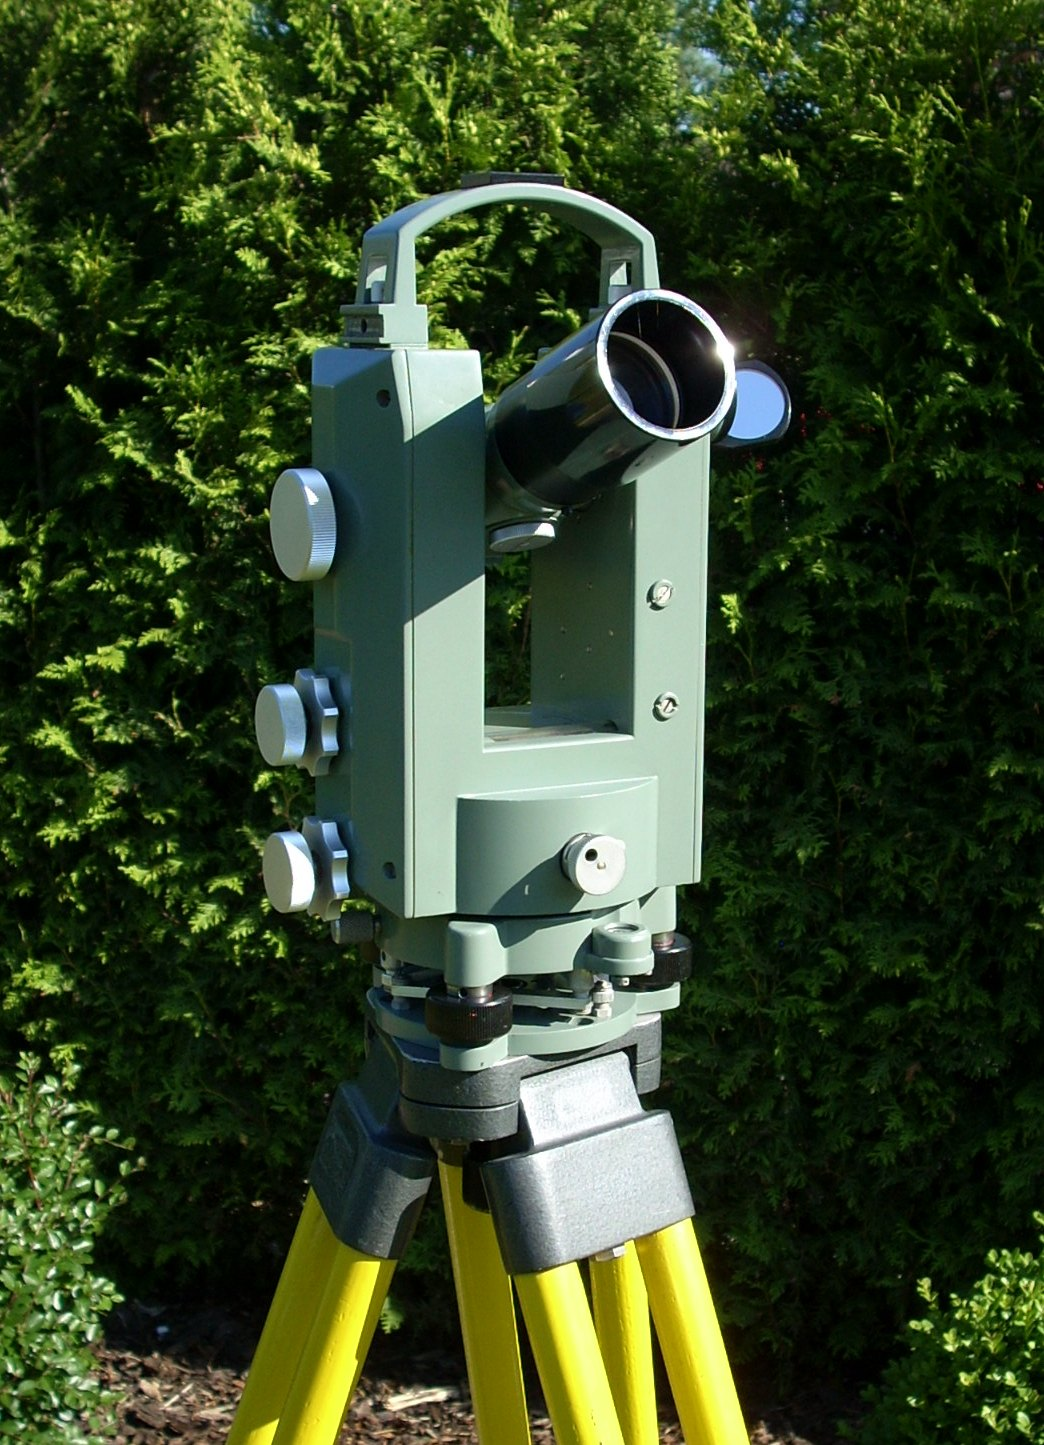
\includegraphics[width=.5\linewidth]{3_gonio_complexe_getallen/inputs/Askania_Sekunden-Theodolit_TU_e_400.jpg}
%\end{center}
%\end{figure}

(Bron figuur: \url{https://commons.wikimedia.org/wiki/File:Askania_Sekunden-Theodolit_TU_e_400.jpg})\\

De staalconstructie van een hoogspanningsmast is gebaseerd op driehoeken.

\gewonefiguur{height=7cm}{3_gonio_complexe_getallen/inputs/Pylon_ds.jpg}

%\begin{figure}[h]
%\begin{center}
%\includegraphics[width=.5\linewidth]{3_gonio_complexe_getallen/inputs/Pylon_ds.jpg}
%\end{center}
%\end{figure}

(Bron figuur: \url{https://commons.wikimedia.org/wiki/File:Pylon_ds.jpg}).\\

In de volgende paragrafen bespreken we praktisch de basis van goniometrie en driehoeksmeetkunde.\\

\subsection{Meten van hoeken}

%\begin{itemize}
%	\item Wat zijn de verschillende manieren om hoeken te meten?
%	\item Hoe kan je overgaan van de ene hoekmaat naar de andere?
%\end{itemize}

\subsubsection{Graden, minuten, seconden}

Een hoekmaat wordt bepaald door een hoek voor te stellen op een cirkel met willekeurige straal $r$ waarbij men de top van de hoek laat samenvallen met het middelpunt van de cirkel. Elke hoek $\alpha$ komt dan overeen met een zekere afstand gemeten langs de omtrek van de cirkel. Men zegt dat met elke hoek $\alpha$ een zekere booglengte op de cirkel met straal $r$ overeenkomt.

\gewonefiguur{scale=.5}{3_gonio_complexe_getallen/inputs/goncirkelhoek-1.pdf}

%\begin{figure}[h]
%\begin{center}
%\includegraphics[scale=.5]{3_gonio_complexe_getallen/inputs/goncirkelhoek-1.pdf}
%\end{center}
%\end{figure}

Door nu de cirkelomtrek onder te verdelen in allemaal stukjes met gelijke booglengte bekomt men een maat voor een hoek. Op de figuur hieronder zijn enkele onderverdelingen getekend.

\gewonefiguur{scale=.37}{3_gonio_complexe_getallen/inputs/graden1.jpg}

%\begin{figure}[h]
%\begin{center}
%\includegraphics[scale=.37]{3_gonio_complexe_getallen/inputs/graden1.jpg}
%\end{center}
%\end{figure}

Deze onderverdelingen noemt men graden. Meestal (maar niet altijd!) wordt een cirkel onderverdeeld in $360^\circ$: een rechte hoek komt dan overeen met $90^\circ$ en een gestrekte hoek met $180^\circ$. Hieronder staan enkele tekeningen:

\gewonefiguur{scale=.5}{3_gonio_complexe_getallen/inputs/hoekendeg.pdf}

%\begin{figure}[h]
%\begin{center}
%\includegraphics[scale=.5]{3_gonio_complexe_getallen/inputs/hoekendeg.pdf}
%\end{center}
%\end{figure}

Graden zijn zelf ingedeeld in minuten (zoals meters kunnen ingedeeld worden in centimeters) en minuten kunnen op hun beurt worden ingedeeld in seconden (zoals centimeters kunnen worden ingedeeld in millimeters).  Graden, minuten en seconden worden echter ingedeeld in een $60$-tallig talstelsel, waardoor je volgende regels krijgt:

\begin{align*}
	1 \textrm{ graad} &= 60 \textrm{ minuten}\\
	1 \textrm{ minuut} &= 60 \textrm{ seconden}
\end{align*}

Deze hoekmaat noemt men de zestigdelige graad. De zestigdelige graad wordt soms afgekort als 'deg' van het Engelse woord 'degree'.\\
Graden, minuten en seconden hebben hun eigen eenheid/symbool, zoals het symbool voor centimeter 'cm' is:

\begin{align*}
	1 \textrm{ graad} &= 1^\circ\\
	1 \textrm{ minuut} &= 1'\\
	1 \textrm{ seconde} &= 1''
\end{align*}

Enkele voorbeelden:

\begin{itemize}
	\item Een hoek van $1^\circ$ lees je als een hoek van '$1$ graad'. Ze bestaat zelf uit $1\cdot 60 = 60$ minuten (want elke graad is $60$ minuten), of uit $60 \cdot 60 = 3600$ seconden (want elke minuut is $60$ seconden).
	\item Een hoek van $42^\circ$ lees je dus als '$42$ graden' en bestaat zelf uit $42 \cdot 60 = 2520$ minuten (want elke graad is $60$ minuten), of uit $2520 \cdot 60 = 151200$ seconden (want elke minuut is $60$ seconden).
	\item Een hoek van $5^\circ12'13"$ lees je als $5$ graden, $12$ minuten en $13$ seconden.
\end{itemize}

Soms wordt het gebruik van minuten en seconden vermeden in de notatie van een hoek, en gebruikt men een decimale notatie. Zo kan het zijn dat je een hoek tegenkomt die genoteerd is als:
\[22,5^\circ \quad \textup{ of ook } \quad 22^\circ,5\]
Dat betekent dan ook letterlijk $22$ en een halve graad. Ofwel $22$ graden en de helft van $60$ minuten. Met andere woorden:
\[22,5^\circ = 22^\circ30'\]
Een tweede, iets moeilijker voorbeeld:

\begin{align*}
42,21^\circ &= 42^\circ+0,21\cdot 1^\circ &\textup{\footnotesize herschrijven van een kommagetal}\\
&= 42^\circ + 0,21 \cdot 60' &\textup{\footnotesize 1 graad is 60 minuten}\\
&= 42^\circ + 12,6' &\textup{\footnotesize uitrekenen}\\
&= 42^\circ + 12' + 0,6\cdot 1' &\textup{\footnotesize herschrijven van een kommagetal}\\
&= 42^\circ + 12' + 0,6 \cdot 60'' &\textup{\footnotesize 1 minuut is 60 seconden}\\
&= 42^\circ + 12' + 36'' & \textup{\footnotesize uitrekenen}\\
&= 42^\circ12'36''
\end{align*}
Gelukkig hebben veel rekentoestellen de mogelijkheid om graden in decimale notatie om te zetten in graden in notatie van graden, minuten, seconden. Raadpleeg daarvoor de handleiding van je rekentoestel.\\

Rekenen met graden, minuten, seconden is anders dan rekenen met tiendelige getallen.  Een voorbeeld:
\[12^\circ45'+36^\circ50'=48^\circ95'=49^\circ35'\]
Telkens als je meer dan $60$ minuten hebt, moet je het aantal graden verhogen met $1$. Net zo bij meer dan $60$ seconden, dan verhoog je het aantal minuten!

\subsubsection{Decimale graad of honderddelige graad}

Zoals eerder gezegd is de onderverdeling van een cirkel in $360^\circ$ alleen maar een afspraak. Volgens een andere conventie wordt een cirkel onderverdeeld in 400 stukjes zodat een rechte hoek overeenkomt met 100 onderverdelingen: men spreekt dan van decimale graden of honderddelige graden.
Honderddelige graden komen vooral voor in de topografie en de weg- en waterbouw. Vooral studenten bouwkunde zullen deze hoekmaat tegen komen. De eenheid van de 100-delige hoek is 'gon' (maar ook 'gr' of 'grad' komen voor). In principe is deze hoekmaat erg eenvoudig. Men start met de afspraak:
\[\textup{Een rechte hoek meet 100 gon.}\]
Bijgevolg zal een getrekte hoek $200$ gon meten, en een hoek van $45^\circ$ de helft van $100$ gon en dus $50$ gon. Honderddelige graden rekenen gemakkelijker dan $60$-delige graden.

\subsubsection{Radialen}

Een andere veel gebruikte hoekmaat is de radiaal. Men neemt een cirkel met straal $r$ en zet daarop een bepaalde hoek uit. Met deze hoek komt dan een welbepaalde booglengte $s$ op de cirkelomtrek overeen. Men zegt nu dat die hoek waarvoor de booglengte $s$ gelijk is aan de straal $r$ een hoek is van 1 radiaal.


\gewonefiguur{scale=0.37}{3_gonio_complexe_getallen/inputs/radiaal1.jpg}

%\begin{figure}[h]
%\begin{center}
%\includegraphics[scale=0.37]{3_gonio_complexe_getallen/inputs/radiaal1.jpg}
%\end{center}
%\end{figure}

Voor een hoek van 2 radialen geldt dus dat $s=2r$, voor een hoek van 5 radialen geldt dan $s=5r$, enz... M.a.w. voor een hoek $\theta$ kan men schrijven dat het verband tussen de cirkelboog $s$ en de straal $r$ gegeven wordt door:

\[ s=r\cdot \theta \]

Let op! Deze formule is all\'{e}\'{e}n geldig als de hoek $\theta$ wordt uitgedrukt in radialen...\\

In theoretische berekeningen (fysica, mechanica,...) wordt bijna altijd ondersteld dat een hoek wordt uitgedrukt in radialen zodat men van deze formule kan gebruik maken.

De omtrek van een cirkel met straal $r$ is de gekende formule $2\cdot \pi \cdot r$. Uit $s=r\cdot \theta$ volgt dan dat de hoek die overeenkomt met de volledige cirkelomtrek gelijk is aan $\theta=2\pi$. Om gemakkelijk te rekenen kiest men dikwijls een cirkel met $r=1$, de omtrek van zo een \'{e}\'{e}nheidscirkel is $2\pi$.  Met dit in het achterhoofd berekenen we de grootte van een rechte hoek ($90^\circ$), maar nu in radialen:

\gewonefiguur{scale=0.75}{3_gonio_complexe_getallen/inputs/rechtehoekrad.pdf}

%\begin{figure}[h]
%\begin{center}
%\includegraphics[scale=0.75]{3_gonio_complexe_getallen/inputs/rechtehoekrad.pdf}
%\end{center}
%\end{figure}

Je ziet dat de rechte hoek een kwart van de cirkel beslaat. De gehele cirkel heeft een omtrek van $2\pi$ en bijgevolg bepaalt de rechte hoek een cirkelboog met lengte $\dfrac{1}{4} \cdot 2\pi = \dfrac{\pi}{2}$.\\ We zeggen:

De rechte hoek meet $\dfrac{\pi}{2}$ radialen.

Op je rekentoestel worden radialen vaak aangegeven met 'rad'. Ook radialen hebben een eenheid, namelijk 'rad'. Vaak laten we deze eenheid weg:
\[90^\circ = \frac{\pi}{2} \text{rad}=\frac{\pi}{2}\]
Het voordeel van radialen is dat deze al kommagetallen zijn, en je ermee kan rekenen zoals je met gewone getallen doet. Het moeilijke is dat radialen vaak 'ongewoon' zijn, omdat het getal $\pi$ er zo vaak in opduikt.  Nog enkele veel voorkomende hoeken:
\begin{itemize}
	\item De nulhoek meet $0^\circ$ en beschrijft geen omtrek op de cirkel (het beginpunt van de cirkelboog is hetzelfde als het eindpunt ervan). Bijgevolg is de nulhoek ook een hoek van $0$ radialen.
	\item De gestrekte hoek meet $180^\circ$ en beschrijft de helft van een cirkel (tekenen!). De omtrek van een halve cirkel is $\pi$ en dus meet de gestrekte hoek $\pi$ radialen.
	\item De volle hoek meet $360^\circ$ en beschrijft de volledige cirkel. De omtrek van de volledige cirkel is $2\pi$ en dus meet de volle hoek $2\pi$ radialen.
\end{itemize}

Volgende regel is zeer belangrijk:
\[180^\circ=\pi\]

Hieruit kan je vaak snel de grootte van een eenvoudige hoek in radialen afleiden. Bijvoorbeeld:
\begin{itemize}
	\item $60^\circ$ is gelijk aan $180^\circ:3$, en dus is de hoek van $60^\circ$ gelijk aan $\dfrac{\pi}{3}$ radialen.
	\item $30^\circ$ is gelijk aan $180^\circ:6$, en dus is de hoek van $30^\circ$ gelijk aan $\dfrac{\pi}{6}$ radialen.
	\item $45^\circ$ is gelijk aan $180^\circ:4$, en dus is de hoek van $45^\circ$ gelijk aan $\dfrac{\pi}{4}$ radialen.
\end{itemize}

Nog even een lijstje formules, waarvan de bovenste de belangrijkste is:

\begin{align*}
180^\circ&=\pi\\
360^\circ&=2\pi\\
90^\circ&=\frac{\pi}{2}\\
60^\circ&=\frac{\pi}{3}\\
45^\circ&=\frac{\pi}{4}\\
30^\circ&=\frac{\pi}{6}
\end{align*}

\subsubsection{Overgangen tussen de verschillende hoekeenheden}

\textbf{Algemeen verband}

De overgang tussen de verschillende hoekeenheden kan je gemakkelijk maken als je weet dat een gestrekte hoek gelijk is aan:

\begin{onthoud}
180$^\circ$=$\pi$ rad=200 gon.
\end{onthoud}

\textbf{Van graden naar radialen en terug}

Omdat $180^\circ = \pi$ rad, zal $1^\circ=\dfrac{180^\circ}{180}=\dfrac{\pi \text{ rad}}{180}$. Je kan dit gebruiken om een willekeurige hoek in graden om te zetten in radialen:
\[32^\circ = 32\cdot 1^\circ = 32 \cdot \frac{\pi}{180} \text{rad}\approx \frac{32\cdot 3,14}{180}\text{rad}=0,56\text{rad}\]
Het is wel erg belangrijk dat je een hoek in graden eerst omzet in een decimale notatie, en niet met minuten en seconden erbij. De regel wordt nu:
\begin{equation*}
x^\circ \textup{ is gelijk aan } x\cdot \frac{\pi}{180} \text{rad}
\end{equation*}
of met andere woorden, omzetten van \textbf{graden naar radialen} is vermenigvuldigen met
\begin{equation*}
\dfrac{\pi}{180}\text{rad}\approx 0,0175\text{rad}
\end{equation*}

Nog een voorbeeldje:
\[42^\circ12'36''=42,21^\circ\approx 42,21 \cdot 0,0175 \text{rad}\approx 0,74 \text{rad}\]

Omdat $\pi \text{rad} = 180^\circ$, vind je dat $1 \text{rad} = \dfrac{\pi}{\pi} \text{  rad}=\dfrac{180^\circ}{\pi}$. Je kan dit gebruiken om een willekeurige hoek in radialen om te zetten in graden:
\[1,35~\text{rad} = 1,35 \cdot 1 \text{rad} = 1,35 \cdot \frac{180^\circ}{\pi}\approx \frac{1,35 \cdot 180^\circ}{3,14}\approx 77,35^\circ\]

Het resultaat is dus altijd een hoek in graden, in decimale notatie.  De algemene regel is dus
\[x \text{rad} \textup{ is gelijk aan } x\cdot \frac{180^\circ}{\pi}\]
of met andere woorden, omzetten van \textbf{radialen naar graden} is vermenigvuldigen met
\[
\frac{180^\circ}{\pi} \approx 57,3^\circ
\]

Nog een voorbeeldje:
\[0,456 \text{rad} \approx 0,456 \cdot 57,3^\circ = 26,13^\circ\]

Merk op dat we bij deze omzettingen vaak afronden. Dat mag enkel als het voor de opgave mag, soms moet je nauwkeurig en symbolisch werken, en dan gebruik je de formules zonder afronden!

\textbf{Van graden naar gon en terug}

We gebruiken de regel dat $90^\circ=100$ gon, dus vind je:
\begin{align*}
1^\circ &= \frac{100 \textup{ gon}}{90}= 1,111 \textup{ gon}\\
1 \textup{ gon} &= \frac{90^\circ}{100} = 0,9^\circ
\end{align*}
Dit gebruik je om de volgende omzettingsregels te vinden:
\begin{align*}
x^\circ &= x\cdot 1,111 \textup{ gon}\\
x \textup{ gon} &= x\cdot 0,9^\circ
\end{align*}

\begin{voorbeeld}
	
\begin{itemize}
	\item $12,13^\circ = 12,13 \cdot 1,111 \textup{ gon} \approx 13,48 \textup{ gon}$.
	\item $78,85 \textup{ gon} = 78,85 \cdot 0,9^\circ \approx 70,97^\circ$
\end{itemize}

\end{voorbeeld}
Ook hier is het belangrijk dat je de decimale notatie van de graden gebruikt, en niet de notatie in minuten en seconden!

\subsubsection{Onthoud}
\ \\
\begin{onthoud}
	\begin{itemize}
\item Hoeken kan je meten in
	
\begin{itemize}
	\item graden ($^\circ$), minuten ('), seconden ('')
	\item radialen (rad), de lengte van een cirkelboog van een cirkel met straal $1$
	\item 100-delige graden(gon)
\end{itemize}
\item $180^\circ=\pi \text{ rad}$
\item $90^\circ=100$ gon
\end{itemize}

Volgende formules zijn zeer nuttig:
\begin{eqnarray*}
x^\circ &=& x\cdot \frac{\pi}{180} \text{rad} \approx x\cdot 0,0175 \text{rad}\\
x \text{rad} &=& x \cdot \frac{180^\circ}{\pi} \approx x \cdot 57,3^\circ\\
x^\circ &=& x \cdot \frac{10}{9} \textup{ gon} \approx x \cdot 1,111 \textup{ gon}\\
x \textup{ gon} &&= x\cdot 0,9^\circ
\end{eqnarray*}
\end{onthoud}


\subsection{Rechthoekige driehoeken}

%\begin{itemize}
%	\item Wat is de stelling van Pythagoras?
%	\item Wat zijn de sinus, cosinus, tangens en cotangens in een rechthoekige driehoek?
%	\item Hoe bereken je hoeken en zijden van een rechthoekige driehoek?
%\end{itemize}

\subsubsection{Tekening en definities}

\gewonefiguur{scale=.5}{3_gonio_complexe_getallen/inputs/driehoek.pdf}

%\begin{figure}[h]
%\begin{center}
%\includegraphics[scale=0.5]{3_gonio_complexe_getallen/inputs/driehoek.pdf}
%\end{center}
%\end{figure}

Een algemene rechthoekige driehoek wordt vaak weergegeven zoals in bovenstaande figuur. Een rechthoekige driehoek bestaat uit zijden en hoeken:
\begin{itemize}
	\item De zijden, aangeduid met de kleine letters $a$, $b$ en $c$.
	\item De hoekpunten $A$, $B$ en $C$.
	\item De hoeken $\alpha$ (alfa) en $\beta$ (beta).
\end{itemize}

De plaats van deze letters wordt meestal op dezelfde manier gedaan:
\begin{itemize}
	\item De rechte hoek krijgt als hoekpunt $C$. De rechte hoek krijgt vaak geen aparte naam, omdat je reeds weet dat deze $90^\circ$ is. Als ze dan toch een naam krijgt, wordt dat $\gamma$ (gamma).
	\item $\alpha$ is de hoek horende bij hoekpunt $A$, $\beta$ is de hoek horende bij hoekpunt $B$.
	\item De zijde tegenover de hoek $\alpha$ is de zijde $a$, en de zijde tegenover de hoek $\beta$ is de zijde $b$. Deze zijden noemt men de \textbf{rechthoekszijden}.
	\item De zijde $c$ ligt tegenover de rechte hoek en het hoekpunt $C$ en wordt de \textbf{hypothenusa} of \textbf{schuine zijde} genoemd.
\end{itemize}

\newpage

\subsubsection{De stelling van Pythagoras}

\begin{center}\textbf{In een rechthoekige driehoek is de 
		som van de kwadraten van de rechthoekszijden gelijk aan het kwadraat van de schuine zijde}\end{center}

\gewonefiguur{scale=.5}{3_gonio_complexe_getallen/inputs/driehoek.pdf}

%\begin{figure}[h]
%\begin{center}
%\includegraphics[scale=0.5]{3_gonio_complexe_getallen/inputs/driehoek.pdf}
%\end{center}
%\end{figure}

Voor deze tekening is dit dan:

\[a^2+b^2=c^2\]

De stelling van Pythagoras is erg nuttig om de zijden van een driehoek te berekenen. Telkens je twee zijden hebt, kan je de derde berekenen.

\subsubsection{Goniometrische getallen in een rechthoekige driehoek}

Aan een hoek $\alpha$ van een rechthoekige driehoek kunnen we een aantal getallen koppelen:
\begin{align*}
\textup{de sinus van }\alpha &=\sin \alpha &= \frac{\textup{overstaande rechthoekszijde}}{\textup{schuine zijde}}\\
&&\\
\textup{de cosinus van }\alpha &=\cos \alpha &= \frac{\textup{aanliggende rechthoekszijde}}{\textup{schuine zijde}}\\
&&\\
\textup{de tangens van }\alpha &=\tan \alpha &= \frac{\textup{overstaande rechthoekszijde}}{\textup{aanliggende rechthoekszijde}}\\
&&\\
\textup{de cotangens van }\alpha &=\cot \alpha &= \frac{\textup{aanliggende rechthoekszijde}}{\textup{overstaande rechthoekszijde}}
\end{align*}

Voor de driehoek

\gewonefiguur{scale=.5}{3_gonio_complexe_getallen/inputs/driehoek.pdf}

%\begin{figure}[h]
%\begin{center}
%\includegraphics[scale=0.5]{3_gonio_complexe_getallen/inputs/driehoek.pdf}
%\end{center}
%\end{figure}

Is dat dan:

\begin{center}
\begin{tabular}{ccccc}
$\sin \alpha$ &$= \dfrac{a}{c}$ &\qquad\qquad\qquad& $\cos \alpha$ &$= \dfrac{b}{c}$\\
&&&&\\
$\tan \alpha$ &$= \dfrac{a}{b}$ &\qquad\qquad\qquad& $\cot \alpha$ &$= \dfrac{b}{a}$
\end{tabular}
\end{center}

Uiteindelijk zijn sinus, cosinus, \ldots van een hoek niet afhankelijk van de driehoek waar je ze in tekent. Daarom kan je ook met je rekentoestel een sinus, cosinus, \ldots berekenen. Zorg wel dat je hoekmaat juist staat ingesteld!

\subsubsection{Nuttige formules}

Volgende formules zijn vaak nuttig om hoeken terug te vinden (met $\sin^2 \alpha$ bedoelen we het kwadraat van de sinus van $\alpha$, of met andere woorden, $(\sin \alpha)^2$):

\begin{align*}
\sin^2 \alpha + \cos^2 \alpha &= 1\\
\tan \alpha &= \frac{\sin \alpha}{\cos \alpha}\\
\cot \alpha &= \frac{\cos \alpha}{\sin \alpha}\\
\tan \alpha\cdot \cot \alpha &= 1
\end{align*}

\textbf{Oplossen van rechthoekige driehoeken}


We hebben enkele formules nodig, studeer deze goed!  Voor een {\bf rechthoekige} driehoek geldt:

\gewonefiguur{scale=.5}{3_gonio_complexe_getallen/inputs/driehoek.pdf}

%\begin{figure}[h]
%\begin{center}
%\includegraphics[scale=0.5]{3_gonio_complexe_getallen/inputs/driehoek.pdf}
%\end{center}
%\end{figure}

\begin{center}
\begin{tabular}{ccccc}
&&$a^2+b^2=c^2$ &&\\
&&&&\\
$\sin \alpha=$ & $\dfrac{a}{c}$ &\qquad\qquad\qquad & $\sin \beta=$ & $\dfrac{b}{c}$\\
&&&&\\
$\cos \alpha=$ & $\dfrac{b}{c}$ &\qquad\qquad\qquad & $\cos \beta=$ & $\dfrac{a}{c}$\\
&&&&\\
$\tan \alpha=$ & $\dfrac{a}{b}$ &\qquad\qquad\qquad & $\tan \beta=$ & $\dfrac{b}{a}$\\
\end{tabular}
\end{center}

Wat kan je hier nu mee? Als je enkele onderdelen van een rechthoekige driehoek gegeven hebt, kan je met deze formules en gegevens de andere onderdelen berekenen. Vaak heb je met $2$ gegeven waarden genoeg. Dit noemen we het oplossen van een rechthoekige driehoek. De bedoeling is $a$, $b$, $c$, $\alpha$ en $\beta$ te bepalen.

\begin{voorbeeld}
	Van de driehoek is gegeven $a = 3$ en $b = 4$. Bereken de overige getallen.\\
Met de stelling van Pythagoras vind je:
\[a^2+b^2=c^2 \Leftrightarrow 3^2+4^2=c^2 \Leftrightarrow 9+16=c^2 \Leftrightarrow 25=c^2 \Leftrightarrow c=5\]
We hebben de $3$ zijden, dus nu moeten we nog de twee hoeken berekenen. Dat doen we met sinus, cosinus, \ldots:
\[\sin \alpha = \frac{a}{c} = \frac{3}{5} = 0,6\]
Nu kan je met je rekentoestel uitrekenen wat $\alpha$ is, vaak met de toets $\sin^{-1}$. Je vindt:
\[\alpha \approx 36,87^\circ\]
Ook $\beta$ kan je vinden op deze manier:
\[\sin \beta = \frac{b}{c}=\frac{4}{5}=0,8\]
En dus
\[\beta \approx 53,13^\circ\]
Zie je dat $\alpha+\beta = 90^\circ$! Dit is geen toeval. De som van de hoeken van een driehoek is $180^\circ$. Omdat je $1$ hoek al kent, namelijk de rechte hoek van $90^\circ$, is de som van de andere $2$ $90^\circ$. Onthoud dus:

\begin{itemize}
	\item \textbf{De som van de hoeken van een driehoek is $180^\circ$}, of met andere woorden
	\[\alpha+\beta+\gamma=180^\circ\]
	\item \textbf{De som van de scherpe hoeken in een rechthoekige driehoek is $90^\circ$}, of m.a.w.
	\[\alpha+\beta = 90^\circ\]
\end{itemize}

\end{voorbeeld}

\begin{voorbeeld}
	Er is gegeven dat $\alpha = 30^\circ$ en $c$ (de schuine zijde) is $7$. Bereken de overige getallen.\\
Je kan meteen $\beta$ vinden:
\[\alpha+\beta=90^\circ \Leftrightarrow 30^\circ + \beta = 90^\circ \Leftrightarrow \beta = 60^\circ\]
De zijden bereken je via een sinus:
\[\sin \alpha = \frac{a}{c}\Leftrightarrow \sin 30^\circ = \frac{a}{7}\Leftrightarrow \frac{1}{2}=\frac{a}{7}\]
Je zondert nu $a$ af door links en rechts met $7$ te vermenigvuldigen en je krijgt:
\[a = \frac{7}{2}\]
De laatste zijde $b$ vind je nu met de stelling van Pythagoras
\[a^2+b^2=c^2 \Leftrightarrow \left(\frac{7}{2}\right)^2+b^2=7^2 \Leftrightarrow 12,25+b^2=49\]
Je zondert $b^2$ af
\[b^2=49-12,25=36,75\]
En dan neem je links en rechts de vierkantswortel
\[b=\sqrt{36,75}\approx 6,06\]
\end{voorbeeld}

De algemene truc is dus telkens een formule te kiezen waar $2$ van de symbolen bekend zijn, om zo het derde te vinden.

\subsubsection{Onthoud}
\begin{onthoud}
	\gewonefiguur{scale=.5}{3_gonio_complexe_getallen/inputs/driehoek.pdf}
%	\begin{figure}[h]
%\begin{center}
%\includegraphics[scale=0.5]{3_gonio_complexe_getallen/inputs/driehoek.pdf}
%\end{center}
%\end{figure}

\begin{itemize}
	\item \textbf{De stelling van Pythagoras}
	\[a^2+b^2=c^2\]
	\item \textbf{sin, cos, tan, cot}
	\begin{center}
\begin{tabular}{ccccc}
$\sin \alpha$ &$= \dfrac{a}{c}$ &\qquad\qquad\qquad& $\cos \alpha$ &$= \dfrac{b}{c}$\\
&&&&\\
$\tan \alpha$ &$= \dfrac{a}{b}$ &\qquad\qquad\qquad& $\cot \alpha$ &$= \dfrac{b}{a}$
\end{tabular}
\end{center}
	\item $\alpha + \beta = 90^\circ$
	\item Een rechthoekige driehoek los je op door formules te kiezen uit Pythagoras, $\sin \alpha, \cos \alpha, \tan\alpha, \sin \beta, \ldots$ waarin twee waarden bekend zijn om zo de derde te vinden.
\end{itemize}
\end{onthoud}


\subsection{Willekeurige driehoeken}

%\begin{itemize}
%	\item Wat is de cosinusregel?
%	\item Wat is de sinusregel?
%	\item Hoe bereken je de zijden en hoeken van een willekeurige driehoek?
%\end{itemize}

\subsubsection{Tekening en afspraken}

\gewonefiguur{scale=.5}{3_gonio_complexe_getallen/inputs/willdriehoek.pdf}

%\begin{figure}[h]
%\begin{center}
%\includegraphics[scale=0.5]{3_gonio_complexe_getallen/inputs/willdriehoek.pdf}
%\end{center}
%\end{figure}

\begin{itemize}
	\item De hoekpunten duiden we aan met $A$, $B$, $C$.
	\item De bijhorende hoeken duiden we aan met $\alpha$ (alfa) bij $A$, $\beta$ (beta) bij $B$ en $\gamma$ (gamma) bij $C$.
	\item De zijde tegenover duiden we aan met $a$ (tegenover $A$), $b$ (tegenover $B$) en $c$ (tegenover $C$).
\end{itemize}

\subsubsection{Sinus- en cosinusregel}

We herinneren er nog eens aan dat de stelling van Pythagoras en de formules voor sinus, cosinus, tangens en cotangens die we tot nu toe besproken hebben all\'{e}\'{e}n geldig zijn voor rechthoekige driehoeken.\\ Voor een willekeurige driehoek gelden iets ingewikkelder formules die de sinusregel en de cosinusregel genoemd worden.\\

De \textbf{cosinusregel:}

\gewonefiguur{scale=.5}{3_gonio_complexe_getallen/inputs/willdriehoek.pdf}

%\begin{figure}[h]
%\begin{center}
%\includegraphics[scale=0.5]{3_gonio_complexe_getallen/inputs/willdriehoek.pdf}
%\end{center}
%\end{figure}

\begin{align*}
a^2&= b^2+c^2-2bc\cos \alpha\\
b^2&=a^2 + c^2 - 2ac\cos \beta\\
c^2&= a^2 + b^2 -2ab \cos \gamma
\end{align*}

Je ziet dat in het linkerlid altijd $1$ bepaalde zijde voorkomt, dat er in het rechterlid de twee andere voorkomen, samen met de cosinus van de hoek die hoort bij het linkerlid. Vergeet zeker de $-2$ niet bij de cosinus!\\

{\bf Opmerking:} als \'{e}\'{e}n van de hoeken een rechte hoek is, bijvoorbeeld de hoek $\alpha=90^\circ$, dan is $\cos \alpha =1$ en vereenvoudigt de cosinusregel tot de stelling van Pythagoras: $a^2=b^2 +c^2$.

De \textbf{sinusregel:}

\[\frac{a}{\sin \alpha}=\frac{b}{\sin \beta}=\frac{c}{\sin \gamma}\]

De sinusregel splits je meestal op in
\begin{align*}
\frac{a}{\sin \alpha} &= \frac{b}{\sin \beta}\\
\frac{a}{\sin \alpha} &= \frac{c}{\sin \gamma}\\
\frac{b}{\sin \beta} &= \frac{c}{\sin \gamma}
\end{align*}

Een andere vorm van de sinusregel is:

\begin{align*}
\frac{\sin \alpha}{a} &= \frac{\sin \beta}{b}\\
\frac{\sin \alpha}{a} &= \frac{\sin \gamma}{c}\\
\frac{\sin \beta}{b} &= \frac{\sin \gamma}{c}
\end{align*}

\subsubsection{Oplossen van willekeurige driehoeken}

Het oplossen van een willekeurige driehoek doe je op dezelfde manier als het oplossen van een rechthoekige driehoek, al zijn de formules anders.  Vergeet ook niet dat de som van de hoeken van een driehoek $180^\circ$ is! We gebruiken in dit onderdeel volgende tekening voor de aanduidingen:

\gewonefiguur{scale=.5}{3_gonio_complexe_getallen/inputs/willdriehoek.pdf}

%\begin{figure}[h]
%\begin{center}
%\includegraphics[scale=0.5]{3_gonio_complexe_getallen/inputs/willdriehoek.pdf}
%\end{center}
%\end{figure}

\[\alpha + \beta + \gamma = 180^\circ\]

Bij een willekeurige driehoek heb je ook meestal meer gegevens nodig dan bij een rechthoekige driehoek om hem op te lossen.  De techniek blijft hetzelfde:
\begin{center}
\textbf{Kies een formule waar $3$ onderdelen gegeven zijn, en bepaal de vierde.}
\end{center}

\begin{voorbeeld}
	In een willekeurige driehoek zijn gegeven $\alpha=20^\circ$, $\gamma = 50^\circ$ en $a=10$. Geef de andere waarden.\\
We moeten dus nog $\beta$, $b$ en $c$ berekenen. Omdat je al twee hoeken hebt, is de derde gemakkelijk te vinden uit:
\[\alpha+\beta+\gamma=180^\circ\Leftrightarrow 20^\circ + \beta + 50^\circ=180^\circ \Leftrightarrow \beta = 110^\circ\]
Om $b$ te berekenen, kunnen we de cosinusregel niet gebruiken, want we kennen $2$ zijden niet, en bij de cosinusregel treden altijd alle zijden op. Dus moeten we de sinusregel gebruiken:
\[\frac{a}{\sin \alpha} = \frac{b}{\sin \beta} = \frac{c}{\sin \gamma}\]
We kennen zowel $a$ als $\alpha$, dus gebruiken we van de sinusregel:
\[\frac{a}{\sin \alpha} = \frac{c}{\sin \gamma}\Leftrightarrow \frac{10}{\sin 20^\circ}=\frac{c}{\sin 50^\circ}\]
Je ziet dat er nog maar $1$ onbekende is, namelijk $c$.  Dus we vinden, door alles uit te rekenen:
\[\frac{10}{0,34}=\frac{b}{0,77}\Leftrightarrow c= \frac{10}{0,34}\cdot 0,77 \approx 22,65\]
Blijft er nog $b$ over, die we ook doen met de sinusregel:
\[\frac{a}{\sin \alpha}=\frac{b}{\sin \beta}\Leftrightarrow \frac{10}{0,34}=\frac{c}{0,94}\Leftrightarrow b= 27,65\]
\end{voorbeeld}

\begin{voorbeeld}
	In een willekeurige driehoek zijn gegeven $\beta = 45^\circ$, $a = 5$, $c=6$. Bepaal de andere waarden.\\
Hier hebben we slechts $1$ hoek, dus de som van de hoeken van een driehoek zal ons niet helpen. Ook met de sinusregel zijn we niet veel, omdat we teveel gegevens missen. Dus blijft er over: de cosinusregel. Welke neem je dan? Die waar $\beta$, $a$ en $c$ in staan:
\[b^2=a^2+c^2-2ac\cos\beta \Leftrightarrow b^2 = 25+36-2\cdot5\cdot 6\cos 45^\circ \Leftrightarrow b^2 = 61-60 \cdot 0,71 \approx 18,4\]
Dus neem je aan beide kanten een vierkantswortel en vind je:
\[b \approx 4,29\]
Nu je $b$ kent, en $\beta$ ook, kan je met de sinusregel $\alpha$ vinden:
\[\frac{\sin \beta}{b}=\frac{\sin \alpha}{a}\Leftrightarrow \frac{\sin 45^\circ}{4,29}=\frac{\sin \alpha}{5}\]
Afzonderen en uitrekenen, levert je dan op
\[\sin \alpha = \frac{45^\circ}{4,29}\cdot 5 = 0,82\]
Je kan nu met $\sin^{-1}$ het juiste antwoord vinden:
\[\alpha=55,08^\circ\]
$\gamma$ vind je nu met
\[\alpha+\beta+\gamma=180^\circ\Leftrightarrow 55,08^\circ + 45^\circ + \gamma = 180^\circ \Leftrightarrow \gamma = 79,92^\circ\]
\end{voorbeeld}


\begin{opmerking}
	\ \\
	
	\begin{itemize}
        \item De som van de hoeken van een driehoek is $180^\circ$, elke hoek apart heeft een grootte tussen $0^\circ$ en $180^\circ$.
		\item Bij het berekenen van de hoeken in een driehoek zal je gebruik maken van de commando's $\sin^{-1}$ en $\cos^{-1}$ op je rekentoestel. Bij gebruik van $\cos^{-1}$ zal dit de juiste hoek geven maar bij gebruik van $\sin^{-1}$ kan dit een verkeerde uitkomst geven. Dit komt omdat $\sin(180^\circ -\alpha)=\sin\alpha$ en het commando $\sin^{-1}$ steeds die hoek oplevert die kleiner is dan $90^\circ$.\\ Bijvoorbeeld: $\alpha = 45^\circ$ en $180^\circ-45^\circ = 135^\circ$ hebben dezelfde sinus. Als de onbekende hoek in de driehoek $135^\circ$ is zal $\sin^{-1}$ echter $45^\circ$ geven... \\
Praktisch ga je bij gebruik van $\sin^{-1}$ bij het oplossen van driehoeken als volgt te werk:	
	
\begin{itemize}
	\item Indien je een meetkundig correcte tekening van de driehoek hebt kan je zien of de hoek die je berekent groter of kleiner dan $90^\circ$ is. Als de hoek die je berekent met $\sin^{-1}$ groter is dan $90^\circ$ vervang dan je uitkomst $\alpha$ door $180^\circ -\alpha$.
	\item Indien je niet zeker bent van de tekening dan controleer je of de som van de hoeken van de driehoek $180^\circ$ is. Als dat niet het geval is vervang dan je uitkomst $\alpha$ door $180^\circ -\alpha$.
\end{itemize}
	
\end{itemize}
\end{opmerking}

\begin{onthoud}
	\ \\
%\begin{figure}[h]
%\begin{center}
%\includegraphics[scale=0.5]{3_gonio_complexe_getallen/inputs/willdriehoek.pdf}
%\end{center}
%\end{figure}

\begin{itemize}
	\item \textbf{De sinusregel}
	\[\frac{a}{\sin \alpha}=\frac{b}{\sin \beta}=\frac{c}{\sin \gamma}\]
	\item \textbf{De cosinusregel}
	\begin{align*}
a^2&= b^2+c^2-2bc\cos \alpha\\
b^2&=a^2 + c^2 - 2ac\cos \beta\\
c^2&= a^2 + b^2 -2ab \cos \gamma
\end{align*}
\item Bij het oplossen van een willekeurige driehoek, neem je best formules waar alle gegevens behalve $1$ kan ingevuld worden.
\item Pas op met de sinus en $\sin^{-1}$
\end{itemize}

\gewonefiguur{scale=.5}{3_gonio_complexe_getallen/inputs/willdriehoek.pdf}

\end{onthoud}

\subsection{De goniometrische cirkel}

%\begin{itemize}
%	\item Hoe teken je de goniometrische cirkel?
%	\item Waar bevinden zich de sinus, cosinus, tangens en cotangens op de goniometrische cirkel?
%	\item Wat zijn de kwadranten in de goniometrische cirkel?
%\end{itemize}

\subsubsection{Tekening}

In een vorig hoofdstukk hebben we de goniometrische getallen van hoeken ingevoerd met behulp van een rechthoekige driehoek. We kunnen ze echter ook voorstellen op een cirkel. We tekenen een cirkel met straal $1$ die met zijn middelpunt in de oorsprong van een orthonormaal* assenstelsel ligt. Deze cirkel noemen we de goniometrische cirkel.
\begin{figure}[h]
\begin{center}
\includegraphics[scale=0.4]{3_gonio_complexe_getallen/inputs/goncirkelleeg.pdf}
\end{center}
\end{figure}

*: een orthonormaal assenstelsel is een rechthoekig (orthogonaal) assenstelsel waarbij de eenheid op beide assen gelijk is.

In de goniometrische cirkel kan je nu een hoek $\alpha$ tekenen, die zijn beginbeen heeft op de $x$-as, en zijn hoekpunt in de oorsprong. Zijn eindbeen snijdt de goniometrische cirkel in een punt $P$ dat we het beeldpunt van de hoek $\alpha$ op de goniometrische cirkel noemen.

\begin{figure}[h]
\begin{center}
\includegraphics[scale=0.4]{3_gonio_complexe_getallen/inputs/goncirkelhoek.pdf}
\end{center}
\end{figure}

Elk punt van de goniometrische cirkel wordt zo het beeldpunt van een hoek door als beginbeen de $x$-as te nemen, als hoekpunt de oorsprong, en als eindbeen de halve rechte door de oorsprong en het punt. De hoek die bij het beeldpunt hoort is niet uniek, integendeel, tel je bij de hoek een aantal volledige omwentelingen op (of trek je die ervan af), dan kom je op hetzelfde beeldpunt terecht. Op die manier hoort bij elk punt van de goniometrische cirkel een oneindig aantal hoeken die onderling een geheel aantal omwentelingen van elkaar verschillen.
In het algemeen spreken we van omwentelingshoeken. Omwentelingshoeken hebben een oriëntatie, in tegenuurwijzerzin is een hoek positief, in uurwijzerzin negatief.


\begin{figure}[h]
	\begin{center}
		\includegraphics[scale=0.4]{3_gonio_complexe_getallen/inputs/omwentelingshoeken.PNG}
	\end{center}
\end{figure}

\subsubsection{Kwadranten}

De goniometrische cirkel wordt ingedeeld in kwadranten.
Ze zijn genummerd, meestal in Romeinse cijfers, tegenkloksgewijs, beginnend rechtsboven in de cirkel.

\gewonefiguur{scale=.5}{3_gonio_complexe_getallen/inputs/goncirkelproj-suppl.jpg}

\subsubsection{Goniometrische getallen}

We kennen de goniometrische getallen als verhoudingen van zijden in een rechthoekige driehoek:

\begin{align*}
\sin \alpha &= \frac{\textup{overstaande rechthoekszijde}}{\textup{schuine zijde}} &\qquad & \cos \alpha &= \frac{\textup{aanliggende rechthoekszijde}}{\textup{schuine zijde}}\\
&&\\
\tan \alpha &= \frac{\textup{overstaande rechthoekszijde}}{\textup{aanliggende rechthoekszijde}}&\qquad &\cot \alpha &= \frac{\textup{aanliggende rechthoekszijde}}{\textup{overstaande rechthoekszijde}}\\
\end{align*}

Scherpe hoeken hebben een beeldpunt in het eerste kwadrant, daarmee kunnen we kunnen een rechthoekige driehoek tekenen in de goniometrische cirkel laten overeenkomen, met zijden $a$, $b$ en $c$:

\gewonefiguur{scale=.5}{3_gonio_complexe_getallen/inputs/goncirkel3hoek.pdf}

%\begin{figure}[h]
%\begin{center}
%\includegraphics[scale=0.5]{3_gonio_complexe_getallen/inputs/goncirkel3hoek.pdf}
%\end{center}
%\end{figure}

In deze rechthoekige driehoek kan je nu de sinus en de cosinus berekenen:
\[\sin \alpha = \frac{a}{c} \qquad \cos \alpha = \frac{b}{c}\]
Je weet dat de lengte van zijde $c$ gelijk is aan $1$, omdat $c$ net de straal is van de goniometrische cirkel! Dus:
\[\sin \alpha = a \qquad \cos \alpha = b\]
De waarde van de sinus kan je dus aflezen op de $y$-as, en de waarde van de cosinus lees je af op de $x$-as, als je het punt $P$ ernaar projecteert.

\gewonefiguur{scale=.6}{3_gonio_complexe_getallen/inputs/goncirkelproj.pdf}

%\begin{center}
%\includegraphics[scale=0.6]{3_gonio_complexe_getallen/inputs/goncirkelproj.pdf}
%\end{center}

Ook de tangens en cotangens kan je aflezen van de goniometrische cirkel.

\gewonefiguur{scale=.6}{3_gonio_complexe_getallen/inputs/goncirkeltancot.pdf}

%\begin{center}
%\includegraphics[scale=0.6]{3_gonio_complexe_getallen/inputs/goncirkeltancot.pdf}
%\end{center}

Uit deze twee figuren blijkt duidelijk dat de sinus en de cosinus niet kleiner kunnen zijn dan $-1$, en niet groter dan $1$. De tangens en de cotangens hebben deze beperkingen niet.

Wat we tot nu toe gevonden hebben voor hoeken uit het eerste kwadrant veralgemenen we voor alle omwentelingshoeken .
De sinus van een hoek is de loodrechte projectie op de $y$-as van het beeldpunt van de hoek, de cosinus van de hoek is de loodrechte projectie op de $x$-as van het beeldpunt van de hoek.
Ook de tangens en de cotangens van om het even welke hoek wordt afgelezen via de goniometrische cirkel zoals dat voor hoeken uit het eerste kwadrant gebeurt.

%\subsubsection{Kwadranten}
%
%De goniometrische cirkel wordt ingedeeld in kwadranten.
%
%\gewonefiguur{scale=.5}{3_gonio_complexe_getallen/inputs/goncirkelkwadrant.pdf}
%
%%\begin{figure}[h]
%%\begin{center}
%%\includegraphics[scale=0.5]{3_gonio_complexe_getallen/inputs/goncirkelkwadrant.pdf}
%%\end{center}
%%\end{figure}
%
%Ze zijn genummerd, meestal in Romeinse cijfers, tegenkloksgewijs, beginnend rechtsboven in de cirkel.
%\begin{align*}
%\alpha \in \textup{I} &\Leftrightarrow 0^\circ < \alpha < 90^\circ\\
%\alpha \in \textup{II} &\Leftrightarrow 90^\circ < \alpha < 180^\circ\\
%\alpha \in \textup{III} &\Leftrightarrow 180^\circ < \alpha < 270^\circ\\
%\alpha \in \textup{IV} &\Leftrightarrow 270^\circ < \alpha < 360^\circ
%\end{align*}
\begin{opmerking}
	 Bij het bespreken van willekeurige driehoeken hebben we vermeld dat het gebruik van het commando $\sin^{-1}$ op een rekentoestel om een hoek $\alpha$ te bepalen soms een verkeerd resultaat kan opleveren. Hieronder is op een figuur gedemonstreerd dat een hoek $\alpha$ uit het eerste kwadrant en een hoek $180^\circ -\alpha$ uit het tweede kwadrant dezelfde sinus hebben. De punten P en Q hebben immers dezelfde projectie op de $y$-as.
\end{opmerking}

\gewonefiguur{scale=.5}{3_gonio_complexe_getallen/inputs/goncirkelproj-suppl.jpg}
%\begin{figure}[h]
%\begin{center}
%\includegraphics[scale=0.5]{3_gonio_complexe_getallen/inputs/goncirkelproj-suppl.jpg}
%\end{center}
%\end{figure}

\begin{onthoud}
	\ \\
	\begin{itemize}
	\item De goniometrische cirkel is een cirkel met straal $1$ met als middelpunt de oorsprong van een orthornormaal assenkruis.
	\item Elk punt van de goniometrische cirkel is het beeldpunt van oneindig veel hoeken die elk een geheel aantal volledige omwentelingen van elkaar verschillen.
	\item De goniometrische getallen van elke hoek kan je aflezen van de goniometrische cirkel:
	\gewonefiguur{scale=.6}{3_gonio_complexe_getallen/inputs/goncirkeltotaal.pdf}
%	\begin{center}
%\includegraphics[scale=0.6]{3_gonio_complexe_getallen/inputs/goncirkeltotaal.pdf}
%\end{center}
	\item De kwadranten verdelen de goniometrische cirkels in $4$ sectoren:
	\gewonefiguur{scale=0.6}{3_gonio_complexe_getallen/inputs/goncirkelkwadrant.pdf}
%	\begin{center}
%\includegraphics[scale=0.6]{3_gonio_complexe_getallen/inputs/goncirkelkwadrant.pdf}
%\end{center}
\begin{align*}
\alpha \in \textup{I} &\Leftrightarrow 0^\circ < \alpha < 90^\circ\\
\alpha \in \textup{II} &\Leftrightarrow 90^\circ < \alpha < 180^\circ\\
\alpha \in \textup{III} &\Leftrightarrow 180^\circ < \alpha < 270^\circ\\
\alpha \in \textup{IV} &\Leftrightarrow 270^\circ < \alpha < 360^\circ
\end{align*}
\end{itemize}

\end{onthoud}

\subsection{Bijzondere hoeken en aanverwante hoeken}

In volgende tabel vind je een overzicht van de belangrijkste goniometrische getallen van bijzondere hoeken. Het bewijs voor de waarden van de goniometrische getallen van deze bijzondere hoeken laten we hier achterwege. Leer deze tabel uit het hoofd.

\begin{tabular}{c|ccccc}
$x$ &	$0 \text{ rad}$& $\frac{\pi}{6} \text{ rad}$ &	$\frac{\pi}{4} \text{ rad}$ &$\frac{\pi}{3} \text{ rad}$ &	 $\frac{\pi}{2} \text{ rad}$ \\
$x$ &	$0^\circ$&	$30^\circ$	&$45^\circ$&	$60^\circ$&	$90^\circ$\\
\hline
$\sin x$ &	$0$	&$\frac{1}{2}$&	$\frac{\sqrt{2}}{2}$& $\frac{\sqrt{3}}{2}$&	$1$ \\
$\cos x$ &	$1$	&$\frac{\sqrt{3}}{2}$&	$\frac{\sqrt{2}}{2}$&	$\frac{1}{2}$&	$0$ \\
$\tan x$ &	$0$	&$\frac{\sqrt{3}}{3}$&	$1$&	$\sqrt{3}$	 &  $|$ \\
\end{tabular}

Uit deze tabel lees je eenvoudig af dat de sinus en de  cosinus van hoeken die samen een rechte hoek vormen eenzelfde waarde hebben. Zo’n hoeken noemen we complementaire hoeken.

We onderscheiden nog andere hoeken waarvan de cosinus en/of de sinus verwant zijn aan elkaar, we noemen ze verwante hoeken. We zetten ze hier allemaal op een rijtje:
\begin{itemize}
	\item complementaire omwentelingshoeken: $\alpha + \beta = 90^\circ= \frac{\pi}{2} \text{ rad}$
	\item omwentelingshoeken met hetzelfde beeldpunt: $\beta = \alpha + 360^\circ; \beta = \alpha + 2 \pi \text{ rad}$
	\item tegengestelde omwentelingshoeken: $\beta = -\alpha$
	\item supplementaire omwentelingshoeken:$\alpha + \beta = 180^\circ; \alpha + \beta = 2 \pi \text{ rad}$
	\item anticomplementaire omwentelingshoeken: $\beta = \alpha + 90^\circ; \beta = \alpha + \frac{\pi}{2} \text{ rad}$
	\item antisupplementaire omwentelingshoeken: $\beta = \alpha + 180^\circ;  \beta = \alpha + \pi \text{ rad}$
\end{itemize}

Het is niet belangrijk om de namen van deze verwante hoeken te kennen, maar wel dat je vanuit een schets van de goniometrische cirkel het verband kan zien tussen de goniometrische getallen van deze hoeken.

Een voorstelling van verwante hoeken van de hoek $\alpha$ vind je in volgende figuur:

\gewonefiguur{scale=.5}{3_gonio_complexe_getallen/inputs/verwanteHoeken.PNG}

\subsection{Overgang van goniometrische getallen van hoeken naar goniometrische functies}

Tot nu toe hebben we steeds goniometrische getallen van hoeken bestudeerd.
Nu definiëren we eveneens de goniometrische getallen van reële getallen.
Definities:
\begin{itemize}
	\item de goniometrische getallen van een reëel getal x, zijn de goniometrische getallen van de hoek x rad
\item het beeldpunt van een reëel getal x op de goniometrische cirkel is het beeldpunt van de hoek x rad op de goniometrische cirkel.
\item de tabel van de goniometrische getallen van bijzondere hoeken geeft een tabel van goniometrische getallen van bijzondere getallen.
\item aanverwante hoeken geven aanleiding tot aanverwante getallen en bijbehorende formules voor hun goniometrische getallen.
\end{itemize}

Door een getal $x$ in $\mathbb{R}$ te laten variëren bekomen we de goniometrische functies (zie mooc wiskunde 2.1.12).

\subsection{Goniometrische formules}

Dit hoofdstuk bestaat uit een opsomming van de belangrijkste formules in goniometrie.

\subsubsection{Bijzondere goniometrische getallen}

\begin{minipage}[b]{0.5\linewidth}
\begin{eqnarray*}
&&\tan \alpha = \frac{\sin \alpha}{\cos \alpha}\\
&&\\
&&\cot \alpha = \frac{\cos \alpha}{\sin \alpha}
\end{eqnarray*}
\end{minipage}
\hspace{0.5cm}
\begin{minipage}[b]{0.5\linewidth}
\begin{eqnarray*}
&&\textup{sec }\alpha = \frac{1}{\cos \alpha}\\
&&\\
&&\textup{csc }\alpha = \frac{1}{\sin \alpha}
\end{eqnarray*}
\end{minipage}

\subsubsection{Grondformules}

\begin{minipage}[b]{0.5\linewidth}
\begin{eqnarray*}
&&\cos^2\alpha +\sin^2 \alpha =1\\
&&1+\tan^2\alpha= \frac{1}{\cos^2 \alpha} = \sec^2 \alpha\\
&&1+\cot^2\alpha = \csc^2 \alpha
\end{eqnarray*}
\end{minipage}

\subsubsection{Verwante hoeken}
\vspace{0.2cm}
\begin{minipage}[b]{0.5\linewidth}
\textbf{Gelijke hoeken}
\begin{eqnarray*}
\sin(\alpha + k\cdot 360^\circ) &=& \sin(\alpha)\\
\cos(\alpha + k\cdot 360^\circ) &=& \cos(\alpha)\\
\tan(\alpha + k\cdot 360^\circ) &=& \tan(\alpha)\\
\cot(\alpha + k\cdot 360^\circ) &=& \cot(\alpha)
\end{eqnarray*}
\end{minipage}
\hspace{0.5cm}
\begin{minipage}[b]{0.5\linewidth}
\textbf{Tegengestelde hoeken}
\begin{eqnarray*}
\sin(-\alpha) &=& -\sin(\alpha)\\
\cos(-\alpha) &=& \cos(\alpha)\\
\tan(-\alpha) &=& -\tan(\alpha)\\
\cot(-\alpha) &=& -\cot(\alpha)
\end{eqnarray*}
\end{minipage}
\ \\
\begin{minipage}[b]{0.5\linewidth}
\textbf{Supplementaire hoeken}
\begin{eqnarray*}
\sin(180^\circ-\alpha) &=& \sin(\alpha)\\
\cos(180^\circ-\alpha) &=& -\cos(\alpha)\\
\tan(180^\circ-\alpha) &=& -\tan(\alpha)\\
\cot(180^\circ-\alpha) &=& -\cot(\alpha)
\end{eqnarray*}
\end{minipage}
\hspace{0.5cm}
\begin{minipage}[b]{0.5\linewidth}
\textbf{Antisupplementaire hoeken}
\begin{eqnarray*}
\sin(\alpha+180^\circ) &=& -\sin(\alpha)\\
\cos(\alpha+180^\circ) &=& -\cos(\alpha)\\
\tan(\alpha+180^\circ) &=& \tan(\alpha)\\
\cot(\alpha+180^\circ) &=& \cot(\alpha)
\end{eqnarray*}
\end{minipage}
\ \\
\begin{minipage}[b]{0.5\linewidth}
\textbf{Complementaire hoeken}
\begin{eqnarray*}
\sin\left(90^\circ-\alpha\right) &=& \cos(\alpha)\\
\cos\left(90^\circ-\alpha\right) &=& \sin(\alpha)\\
\tan\left(90^\circ-\alpha\right) &=& \cot(\alpha)\\
\cot\left(90^\circ-\alpha\right) &=& \tan(\alpha)
\end{eqnarray*}
\end{minipage}
\hspace{0.5cm}
\begin{minipage}[b]{0.5\linewidth}
\textbf{Anticomplementaire hoeken}
\begin{eqnarray*}
\sin\left(90^\circ+\alpha\right) &=& \cos(\alpha)\\
\cos\left(90^\circ+\alpha\right) &=& -\sin(\alpha)\\
\tan\left(90^\circ+\alpha\right) &=& -\cot(\alpha)\\
\cot\left(90^\circ+\alpha\right) &=& -\tan(\alpha)
\end{eqnarray*}
\end{minipage}

\subsubsection{Som- en verschilformules}

\begin{minipage}[b]{0.6\linewidth}
\begin{eqnarray*}
&&\sin(\alpha \pm \beta) = \sin\alpha\cos\beta \pm \cos\alpha\sin\beta\\
&&\cos(\alpha \pm \beta) = \cos\alpha\cos\beta \mp \sin\alpha\sin\beta\\
&&\tan(\alpha \pm \beta) = \frac{\tan\alpha\pm\tan\beta}{1\mp \tan\alpha\tan\beta} \\
&&\cot(\alpha \pm \beta) = \frac{\cot \alpha \cot\beta \mp 1}{\cot \alpha \pm \cot \beta}
\end{eqnarray*}
\end{minipage}

\subsubsection{Verdubbelingsformules}

\begin{minipage}[b]{0.5\linewidth}
\begin{eqnarray*}
\sin2\alpha &=& \frac{2\tan\alpha}{1+\tan^2\alpha}\\
\tan2\alpha &=& \frac{2\tan \alpha}{1-\tan^2\alpha}
\end{eqnarray*}
\end{minipage}
\hspace{0.5cm}
\begin{minipage}[b]{0.5\linewidth}
\begin{eqnarray*}
\cos2\alpha &=& \frac{1-\tan^2\alpha}{1+\tan^2\alpha}\\
&=& 1-2\sin^2\alpha\\
&=& 2\cos^2\alpha-1
\end{eqnarray*}
\end{minipage}

\subsubsection{Simpson-formules}

\begin{eqnarray*}
\sin(x)+\sin(y)&=&2\sin\frac{x+y}{2}\cos\frac{x-y}{2}\\
\sin(x)-\sin(y)&=&2\cos\frac{x+y}{2}\sin\frac{x-y}{2}\\
\cos(x)+\cos(y)&=&2\cos\frac{x+y}{2}\cos\frac{x-y}{2}\\
\cos(x)-\cos(y)&=&-2\sin\frac{x+y}{2}\sin\frac{x-y}{2}
\end{eqnarray*}

\subsubsection{Omgekeerde Simpson-formules}

\begin{eqnarray*}
\sin\alpha\cos\beta&=&\frac{1}{2}\left[\sin(\alpha + \beta)+\sin(\alpha - \beta)\right]\\
\cos\alpha\cos\beta&=&\frac{1}{2}\left[\cos(\alpha + \beta)+\cos(\alpha - \beta)\right]\\
\sin\alpha\sin\beta&=&-\frac{1}{2}\left[\cos(\alpha + \beta)-\cos(\alpha - \beta)\right]
\end{eqnarray*}

\subsection{Oplossen van goniometrische vergelijkingen in $\mathbb{R}$}

Bij het oplossen van goniometrische vergelijkingen zoek je alle reële getallen die aan de vergelijking voldoen. Het spreekt vanzelf dat je dan ook gebruik zal moeten maken van verwante getallen die je terugvindt via de goniometrische cirkel. 
Het is de bedoeling om elke goniometrische vergelijking te herleiden tot één of meerdere basisvergelijkingen.

Basisvergelijkingen:
\begin{itemize}
	\item $\cos(x)=\cos(a) \iff x = \pm a+2k \pi \text{ met } k\in \mathbb{Z} $
	\item $\sin(x)=\sin(a) \iff x = a+2k  \pi  \text{ of } x=\pi-a+2 k \pi \text{ met } k \in \mathbb{Z} $
	\item $\tan(x)=\tan(a)\iff x = a+k \pi \text{ met } k\in \mathbb{Z} $ 
\end{itemize}


\begin{voorbeeld}
$\sin(x)=\frac{1}{2} \iff x=\frac{\pi}{6}+2k \pi \text{ of } x= \frac{5\pi}{6}+2 k \pi \text{ met } k\in \mathbb{Z} $
\end{voorbeeld}
\begin{voorbeeld}
$\cos(x)=0,7 \iff x=\pm 0,795+2k \pi \text{ met } k\in \mathbb{Z} $
\end{voorbeeld}
\begin{voorbeeld}
$\tan(x)=-1,5 \iff x=- 0,983+k \pi \text{ met } k\in \mathbb{Z} $
\end{voorbeeld}
\begin{voorbeeld}
$\sin(x)=1,5 $  : heeft geen oplossingen
\end{voorbeeld}


\subsection{Oefeningen}

\begin{oef}
	Druk uit in radialen:
	\begin{enumerate}
		\item $108,17^\circ$ 
		\item $12^\circ 40' 33''$ 
		\item $190$ gon
	\end{enumerate}
\end{oef}
\oplos{$1,887923$ rad; $0,221235$ rad; $2,984513$ rad (of ook: $\frac{19}{20}\pi$ rad)}

\begin{oef}
	Reken uit:
	\begin{enumerate}
		\item $267,83^\circ - 117,85^\circ$
		\item $12^\circ 02' 58'' + 4^\circ 13' 07''$
		\item $\frac{5}{3}\pi$ rad - $5^\circ 12' 57''$ (in radialen)
		\item $15,15$ gon + $15,15^\circ$ (in decimale graad)
	\end{enumerate}
\end{oef}
\oplos{$149,98^\circ$; $16^\circ 16' 05''$; $5,144954$ rad; $31,9833$ gon}

\subsubsection{Rekenen met driehoeken}

\begin{oef}
Om de hoogte van een mast te bepalen plaatst een landmeter een theodoliet in het punt $P$ op een hoogte $h=1,65$ m. Ze meet dan de hoeken $\alpha$ en $\beta$ met de horizontale: $\alpha=78,12^\circ$ en $\beta=4,71^\circ$.\\
Bereken de hoogte $H$ van de mast.

\gewonefiguur{scale=0.3}{3_gonio_complexe_getallen/inputs/oefn-mast.jpg}

%\begin{figure}[h]
%	\begin{center}
%		\includegraphics[scale=0.30]{\diepte/figures/oefn-mast.jpg}
%	\end{center}
%\end{figure}
\end{oef}
\oplos{$H=96,85$ m}

\begin{oef}
e lengte van elke zijde van de gegeven driehoek zijn gekend: $a=53$ cm, \\ $b=18$ cm en $c=41$ cm.\\
Bereken de hoek $\alpha$.

\gewonefiguur{scale=0.5}{3_gonio_complexe_getallen/inputs/oef-driehoek-1.jpg}
\end{oef}
\oplos{$\alpha=123,01^\circ$ }

\begin{oef}
Bereken de lengte van zijde $c$ van de gegeven driehoek.\\
Gegevens: $a=13$ mm, $b=20$ mm, $\alpha=21^\circ$. 

\gewonefiguur{scale=0.5}{3_gonio_complexe_getallen/inputs/oef-driehoek-2.jpg}
\end{oef}
\oplos{$c=7,83$ mm}

\begin{oef}
	Op de figuur is een schets van een stuk weiland met de gekende gegevens weergegeven. \\
	Bereken de lengte van zijde $d$ en de hoeken $\alpha$ en $\beta$.
	
	\gewonefiguur{scale=0.5}{3_gonio_complexe_getallen/inputs/oef-driehoek-3.jpg}
\end{oef}
\oplos{$d=33,17$ m; $\alpha=147,02^\circ$; $\beta=56,98^\circ$}




\section{Complexe getallen}

%\title{Complexe getallen}

\subsection*{Inleiding}
\addcontentsline{toc}{subsection}{Inleiding}

De verzameling van de complexe getallen $\mathbb{C}$ is een uitbreiding van de verzameling van de re\"{e}le getallen $\mathbb{R}$ waarbij elk complex getal bestaat uit twee re\"{e}le getallen. Het ene re\"{e}el getal wordt het re\"{e}el deel van het complex getal genoemd, het andere re\"{e}el getal het imaginaire deel.\\ 
Alhoewel een eerste kennismaking met complexe getallen heel wat mensen hun wenkbrauwen doet fronsen blijkt dit soort getallen heel wat rekenwerk in de fysica en de techniek eenvoudiger te maken. Dit is bijvoorbeeld zeker het geval in vakgebieden als mechanica (trillingen), akoestiek (golven) en elektrotechniek (wisselstroom).\\

\subsection{De imaginaire eenheid}

\begin{definitie}
	Als eerste stap bij het bespreken van complexe getallen defini\"{e}ren we de imaginaire eenheid $i$ als het getal waarvoor geldt:

\[
i^2 =-1 
\]
\end{definitie}

\begin{opmerking}
	Hierbij moeten we enkele bedenkingen maken:\\
\begin{itemize}
\item Het gebeurt wel eens dat deze definitie wordt herschreven als $i=\sqrt{-1}$. Dit is echter totaal {\bf fout}. We zullen verderop zien dat $-1$ meer dan \'{e}\'{e}n vierkantswortel heeft.
\item In sommige vakgebieden zoals elektrotechniek geeft men de voorkeur aan de letter $j$ als symbool voor de imaginaire eenheid.
\item Een eigenschap van $i$ die heel wat rekenwerk kan vereenvoudigen is het volgende:
\begin{eigenschap}
\begin{equation*}
 i^2=-1 \iff  i=-\frac{1}{i} \iff -i=\frac{1}{i} 
\end{equation*}
\end{eigenschap}

\end{itemize}
\end{opmerking}
\subsection{Het complex getal}

\begin{definitie}
Twee re\"{e}le getallen $x$ en $y$ worden gecombineerd tot een complex getal $z$:
\begin{equation*}
z=x+iy
\end{equation*}
\end{definitie}

Het re\"{e}le getal $x$ wordt het re\"{e}le deel van $z$ genoemd: $x=Re(z)=\Re(z)$.\\
Het re\"{e}le getal $y$ wordt het imaginaire deel van $z$ genoemd: $y=Im(z)=\Im(z)$.\\
Merk op dat als $y=0$ dan $z=x$ met $x \in \mathbb{R}$. Met andere woorden de verzameling van de re\"{e}le getallen is een deelverzameling van de verzameling van de complexe getallen: $\mathbb{R} \subset \mathbb{C}$. Analoog geldt dat als $x=0$ dan $z=iy$. Het getal $iy$ wordt een {\bf imaginair getal} genoemd.\\

Aangezien een complex getal bestaat uit twee re\"{e}le getallen kan een complex getal meetkundig worden voorgesteld door een punt in een vlak. Dit vlak, {\bf het complex vlak}, wordt bepaald door de getallenas van de re\"{e}le getallen, de re\"{e}le as, met loodrecht daarop de imaginaire as. Deze laatste is de re\"{e}le as waarop de eenheid (het getal $1$) vervangen is door $i$.  

\gewonefiguur{scale=0.6}{3_gonio_complexe_getallen/inputs/complex-getal-1.jpg}

%\begin{figure}[h]
%\begin{center}
%\includegraphics[scale=0.6]{3_gonio_complexe_getallen/inputs/complex-getal-1.jpg}
%\end{center}
%\caption{\it Voorstelling van een complex getal $x+iy$ in het complex vlak}
%\end{figure}

Met behulp van schuifknoppen kan je in de volgende interactieve voorstelling het re\"{e}le en imaginaire deel van het getal veranderen en nagaan waar in het complex vlak het complex getal zich bevindt.\\


\begin{minipage}{.25\linewidth}
	\raggedright
	\includegraphics[width=4cm]{3_gonio_complexe_getallen/inputs/QR_Code_ANIMATIE1_module3new}
\end{minipage}
\begin{minipage}{.7\linewidth}
	Scan QR code voor animatie.
\end{minipage}\\

De plaats van een punt in een vlak is ook bepaald door de plaatsvector van het punt. Een complex getal $z$ kan dus ook worden voorgesteld als een vector in het complex vlak. Een dergelijke vector wordt meestal aangeduid met het symbool $\underline{z}$.\\

\gewonefiguur{scale=0.6}{3_gonio_complexe_getallen/inputs/complex-getal-2.jpg}

Een interactieve voorstelling van een vector in het complex vlak.\\

\begin{minipage}{.25\linewidth}
	\raggedright
	\includegraphics[width=4cm]{3_gonio_complexe_getallen/inputs/QR_Code_ANIMATIE2_module3new}
\end{minipage}
\begin{minipage}{.7\linewidth}
	Scan QR code voor animatie.
\end{minipage}  \\

\subsection{Rekenen met complexe getallen}

\subsubsection{Som van complexe getallen}

\begin{definitie}
De som van twee complexe getallen $z_{1}=a+ib$ en $z_{2}=c+id$ is gedefinieerd als\\

\begin{framed}
\[ z_{1}+z_{2}=(a+c)+i(b+d) \]
\end{framed}

ofwel

\begin{framed}
\[	
\begin{array}{ccc}
\Re(z_{1}+z_{2})=\Re(z_{1})+\Re(z_{2}) &  & \Im(z_{1}+z_{2})=\Im(z_{1})+\Im(z_{2}) 
\end{array} 
\]
\end{framed}
\end{definitie}

Het afzonderlijk optellen van de re\"{e}le en imaginaire delen van de complexe getallen kan beschouwd worden als het optellen van componenten van vectoren in het complex vlak. Met andere woorden: optellen van complexe getallen komt neer op optellen van vectoren in het complex vlak.\\

\gewonefiguur{scale=0.6}{3_gonio_complexe_getallen/inputs/complex-getal-3-optelling.jpg}

%\begin{figure}[h]
%	\begin{center}
%		\includegraphics[scale=0.6]{3_gonio_complexe_getallen/inputs/complex-getal-3-optelling.jpg}
%	\end{center}
%\caption{\it Optellen van complexe getallen komt neer op optellen van vectoren in het complex vlak}
%\end{figure}

\subsubsection{Product van complexe getallen}

Als we twee complexe getallen $z_{1}=a+ib$ en $z_{2}=c+id$ met elkaar willen vermenigvuldigen kunnen we dit in eerste instantie neerschrijven als $z_{1} z_{2}=(a+ib)(c+id)$.\\
Om het product te berekenen worden de haakjes uitgewerkt op de klassieke manier maar wordt er expliciet rekening gehouden met $i^2 =-1$.\\

\begin{eigenschap}
	\begin{framed}
\[ z_{1}z_{2}=(a+ib)(c+id)=ac+iad+ibc+i^2 bd=(ac-bd)+i(ad+bc) \]
\end{framed}
\end{eigenschap}

\subsubsection{Complex toegevoegde van een complex getal}

\begin{definitie}
	De complex toegevoegde van een complex getal vindt men door het imaginair deel van een complex getal van teken te veranderen. Men noteert de complex toegevoegde van $z$ als $\overline{z}$.\\
Dus, als $z=x+iy$ dan is de complex toegevoegde van $z$ het getal $\overline{z}=x-iy$.\\
\end{definitie}
\begin{eigenschap}
	Een getal vermenigvuldigen met zijn complex toegevoegde geeft het volgende interessante resultaat:

\begin{framed}
\[ z \overline{z}=(x+iy)(x-iy)=x^2 -ixy+iyx-i^2 y^2=x^2 +y^2 \in \mathbb{R} \]
\end{framed}
\end{eigenschap}

\gewonefiguur{scale=0.6}{3_gonio_complexe_getallen/inputs/complex-getal-4-complex-toegevoegde.jpg}

Een meer interactieve voorstelling vind je hier.\\

\begin{minipage}{.25\linewidth}
	\raggedright
	\includegraphics[width=4cm]{3_gonio_complexe_getallen/inputs/QR_Code_ANIMATIE3_module3new}
\end{minipage}
\begin{minipage}{.7\linewidth}
	Scan QR code voor animatie.
\end{minipage}  \\


\subsubsection{Modulus van een complex getal}

\begin{definitie}
	De grootte van de plaatsvector van een complex getal wordt de modulus van dat getal genoemd. 

\end{definitie}
Met behulp van de stelling van Pythagoras wordt de grootte berekend als $|\underline{z}|=|x+iy|=\sqrt{x^2 +y^2}$.\\
\begin{eigenschap}
	De modulus van het complex getal $z=x+iy$ kan dus ook geschreven worden als

\begin{framed}
\[ |z|=\sqrt{x^2 +y^2}=\sqrt{z \overline{z}}  \]
\end{framed}

\end{eigenschap}

\subsubsection{Quoti\"{e}nt van complexe getallen}

Het berekenen van het quoti\"{e}nt van twee complexe getallen komt er op neer dat men er voor zorgt dat de noemer van de uitdrukking een re\"{e}el getal wordt. De gehele uitdrukking wordt dan een duidelijk leesbaar complex getal.\\
De eenvoudigste manier om dit te doen is teller en noemer vermenigvuldigen met de complex toegevoegde van de noemer.\\
Laten we de getallen $z_{1}=a+ib$ en $z_{2}=c+id$ delen door elkaar:

\begin{framed}
\[ \frac{z_{1}}{z_{2}}=\frac{a+ib}{c+id}=\frac{(a+ib)(c-id)}{(c+id)(c-id)}=\frac{(ac+bd)+i(bc-ad)}{c^2 +d^2}  \]
\end{framed}

\begin{voorbeeld}	
\[ \frac{4-i}{1+i}=\frac{(4-i)(1-i)}{(1+i)(1-i)}=\frac{4-4i-i-1}{2}=\frac{3}{2}-\frac{5}{2}i \]
\end{voorbeeld}

\subsection{Rekenen met complexe getallen - voorbeeld}
\begin{minipage}{.25\linewidth}
	\raggedright
	\includegraphics[width=4cm]{3_gonio_complexe_getallen/inputs/QR_Code_REKENENCOMPLVB_module3new}
\end{minipage}
\begin{minipage}{.7\linewidth}
	Zie filmpje MOOC.
\end{minipage}

\subsection{Goniometrische vorm van een complex getal}

De plaats van een punt $P$ in een vlak wordt traditioneel vastgelegd met behulp van de cartesische co\"{o}rdinaten $(x,y)$. Het is echter evengoed mogelijk hiervoor andere co\"{o}rdinaten te kiezen. Een mogelijk alternatieve keuze zijn de afstand $r$ van het punt $P$ tot de oorsprong en de hoek $\theta$ die de rechte $OP$ maakt met de $x-$as. $(r,\theta)$ worden poolco\"{o}rdinaten genoemd.\\
Passen we dit toe op een complex getal $z$ in het complex vlak dat wordt de afstand $r$ de modulus $|z|$ en de hoek $\theta$ de hoek die de vector $\underline{z}$ maakt met de $x-$as.\\

\begin{figure}[h]
	\begin{center}
		\includegraphics[scale=0.6]{3_gonio_complexe_getallen/inputs/complex-getal-5-goniometrisch.jpg}
	\end{center}
	\caption{\it Goniometrische vorm van een complex getal. De plaats van het getal in het complex vlak wordt vastgelegd door de poolco\"{o}rdinaten $r=|z|$ en $\theta$}
\end{figure}

Door de bij het getal $z=x+iy$ horende vector te projecteren op de re\"{e}le as en op de imaginaire as vindt men

\[ \left\{ \begin{array}{l}
x=\Re(z)=|z|\cos \theta  \\ y=\Im(z)=|z|\sin \theta
\end{array} \right. \]

\begin{eigenschap}
	In goniometrische vorm wordt dat

\begin{framed}
\[ z=x+iy=|z|(\cos \theta + i \sin \theta)   \]
\end{framed}
Met 

\begin{framed}
	\[ \begin{array}{lll}
	\text{modulus van } z=x+iy & & |z|=\sqrt{x^2 +y^2} \\
	\text{argument van } z=x+iy & & \theta = \arctan \frac{y}{x}
	\end{array} \]
\end{framed}

\end{eigenschap}


\begin{opmerking}
\ \\
\begin{itemize}
	\item Een punt in het complex vlak met $r=|z|$ en poolhoek $\theta$ kan ook beschreven worden met dezelfde $r$ maar een poolhoek $\theta+2\pi$, een poolhoek $\theta+ 4\pi$, enz... Men zegt dat de hoek $\theta$ bepaald is op een geheel aantal keer $2\pi$ na.
	\[ z=|z|(\cos \theta + i \sin \theta)=|z|(\cos(\theta +k2\pi)+i \sin(\theta+k2\pi)) \]
	met $k$ een geheel getal.\\
	De hoek waarvoor geldt $\theta \in [0,2\pi[$ is de {\bf hoofdwaarde van het argument}. 
	\item Bij het berekenen van het argument wordt gebruik gemaakt van de Arctan-functie. Het bereik van deze functie is $]-\frac{\pi}{2},\frac{\pi}{2}[$ waardoor het berekende argument het complex getal altijd in het eerste of vierde kwadrant plaatst.\\ 
	{\bf Het is dus zeer belangrijk om te controleren of het complex getal in werkelijkheid niet in het tweede of derde kwadrant ligt. Als dat het geval is moet een correctie op het berekende argument worden toegepast!} \\ We illustreren hoe dit in zijn werk gaat met enkele voorbeelden.
\end{itemize}

\end{opmerking}

	We zetten de volgende complexe getalen in goniometrische vorm: \\
\begin{voorbeeld}


	$z=3+2i$ \\  We maken een figuur om duidelijk te maken in welk kwadrant het getal ligt. \\
	
	\gewonefiguur{scale=0.5}{3_gonio_complexe_getallen/inputs/complex-getal-voorbeeld1.jpg}
	

	Het getal ligt in het eerste kwadrant. We kunnen dus gewoon de formule voor het argument gebruiken zonder correctie.\\
	\[ \begin{array}{lll}
	|z|=\sqrt{3^2 +2^2} & & |z|=\sqrt{13} \\
	\tan \theta = \frac{2}{3} & & \theta = 33,69^{o}\\
	         & &      \\
	z=\sqrt{13} (\cos (33,69^{o}) + i \sin (33,69^{o})  &  &
	\end{array} \]
\end{voorbeeld}
	
\begin{voorbeeld}
	$z=-3-2i$ \\ We maken een figuur om duidelijk te maken in welk kwadrant het getal ligt. \\
	
	\gewonefiguur{scale=0.5}{3_gonio_complexe_getallen/inputs/complex-getal-voorbeeld2.jpg}
	
	Het getal ligt in het derde kwadrant. We moeten dus een correctie toepassen op het berekende argument $\theta$ om het werkelijke argument $\theta^{'}$ te vinden. We tellen  $\pi$ of $180^{o}$ bij het berekende argument. \\
	\[ \begin{array}{lll}
	|z|=\sqrt{(-3)^2 +(-2)^2} & & |z|=\sqrt{13} \\
	\tan \theta = \frac{-2}{-3}=\frac{2}{3} & & \theta = 33,69^{o}\\
	\theta^{'}=\theta+180^{o} & & \theta^{'}=213,69^{o} \\
	&  &          \\
    z=\sqrt{13} (\cos (213,69^{o}) + i \sin (213,69^{o})) &  & 
	\end{array} \]
\end{voorbeeld}
	
\begin{voorbeeld}
	 $z=-3+2i$ \\ We maken een figuur om duidelijk te maken in welk kwadrant het getal ligt. \\

	\gewonefiguur{scale=0.5}{3_gonio_complexe_getallen/inputs/complex-getal-voorbeeld3.jpg}
	
	Het getal ligt in het tweede kwadrant. We moeten dus een correctie toepassen op het berekende argument $\theta$ om het werkelijke argument $\theta^{'}$ te vinden. We tellen  $\pi$ of $180^{o}$ bij het berekende argument. \\
	\[ \begin{array}{lll}
	|z|=\sqrt{(-3)^2 +2^2} & & |z|=\sqrt{13} \\
	\tan \theta = \frac{2}{-3}=-\frac{2}{3} & & \theta = -33,69^{o}\\
	\theta^{'}=\theta+180^{o} & & \theta^{'}=146,31^{o} \\
	&  &          \\
	z=\sqrt{13} (\cos (146,31^{o}) + i \sin (146,31^{o})) &  & 
	\end{array} \]

\end{voorbeeld}

\subsection{De exponenti\"{e}le vorm van een complex getal}

\subsubsection{De formule van Euler}

De formule van Euler drukt uit hoe de functies $\cos$ en $\sin$ in verband staan met de natuurlijke exponenti\"{e}le functie.\\
\begin{eigenschap}
	Voor elk getal $x \in \mathbb{R}$ geldt:\\

\begin{framed}
	\[ e^{ix}=\cos(x) + i \sin(x) \]
\end{framed}
\end{eigenschap}

Deze formule wordt bewezen in de analyse door aan te tonen dat de Taylorreeksontwikkeling van de functie $e^{ix}$ en van de functie $\cos(x) + i \sin(x)$ hetzelfde zijn. \\

\begin{eigenschap}
	Voor praktisch rekenwerk met complexe getallen wordt de formule van Euler neergeschreven als:\\

\begin{framed}
	\[  \begin{array}{l} 
	e^{i \theta}=\cos \theta +i \sin \theta \\
	e^{-i \theta}=\cos \theta - i \sin \theta 
	\end{array}  \]
\end{framed}
Waarbij $\theta$ het argument voorstelt van de goniometrische vorm van een complex getal. \\
\end{eigenschap}

\begin{eigenschap}
	De formule van Euler leidt dus tot een derde, voor de praktijk zeer belangrijke, schrijfwijze voor complexe getallen.\\

\begin{framed}
	\[ \begin{array}{ll}
	\text{de algebra\"{i}sche vorm} & z=x+iy \\
	\text{de goniometrische vorm} & z=|z|(\cos \theta +i \sin \theta) \\
	\textbf{de exponenti\"{e}le vorm} & z=|z|e^{i \theta} \end{array}  \]
\end{framed}

\end{eigenschap}

In principe moet in de formule van Euler, en dus ook in de exponenti\"{e}le vorm van een complex getal, het argument $\theta$ uitgedrukt worden in radialen. Het gebeurt echter dikwijls dat het argument wordt uitgedrukt in graden. Dit is geen probleem zolang men beseft dat om de {\bf numerieke waarde} van bijvoorbeeld $e^{i 45^{o}}$ rechtstreeks te berekenen men $e^{i\frac{\pi}{4}}$ moet uitrekenen.\\
	

\begin{voorbeeld}
	We schrijven het getal $z=-2\sqrt{3}-2i$ in exponenti\"{e}le vorm.\\

\vspace{0.3cm}

Als eerste stap maken we een figuur die het getal voorstelt in het complex vlak.\\

\gewonefiguur{scale=0.5}{3_gonio_complexe_getallen/inputs/complex-getal-voorbeeld4.jpg}

Het getal ligt in het derde kwadrant. Er zal dus een correctie op de berekende waarde voor het argument moeten worden toegepast.\\

\[ \begin{array}{lll}
	|z|=\sqrt{(-2\sqrt{3})^2 +(-2)^2} & & |z|=4 \\
	\tan \theta = \frac{-2}{-2\sqrt{3}}=\frac{1}{\sqrt{3}} & & \theta = 30^{o}\\
	\theta^{'}=\theta+180^{o} & & \theta^{'}=210^{o} \\
	&  &          \\
	z=4e^{i210^{o}} \text{ of ook } z=4e^{i\frac{7}{6}\pi}  &  & 
\end{array} \]

\end{voorbeeld}

\subsection{Bewerkingen in exponenti\"{e}le vorm: som, product en quoti\"{e}nt} 

\subsubsection{De som}

Er bestaat geen snelle manier om twee complexe getallen in exponenti\"{e}le vorm op te tellen. Als je met dit probleem geconfronteerd wordt kan je op twee manieren te werk gaan.\\

{\bf Eerste werkwijze:} \\

\begin{enumerate}
	\item Reken de complexe getallen om naar hun algebra\"{i}sche vorm met behulp van de formule van Euler
	\item Tel de getallen in algebra\"{i}sche vorm op
	\item Zet de som terug om naar exponenti\"{e}le vorm.
\end{enumerate}

\vspace{0.3cm}

{\bf Tweede werkwijze:} \\

Beschouw het optellen van de twee complexe getallen als het optellen van twee vectoren in het complex vlak en gebruik driehoeksmeetkunde om de grootte (modulus) en de ori\"{e}ntatie (argument) van de somvector te bepalen.\\

\vspace{0.3cm}

Beschouw twee complexe getallen $a=|a|e^{i\alpha}$ en $b=|b|e^{i\beta}$ waarvan je de som wil berekenen. Je wil dus modulus en argument van het complex getal $z=a+b=|z|e^{i\theta}$ vinden.\\
Maak nu een figuur waarin je de optelling grafisch voorstelt als de optelling van vectoren in het complex vlak:\\

\figuurmetlabel[\label{fig:compl_som}]{scale=0.6}{3_gonio_complexe_getallen/inputs/complex-getal-6-optelling-exp.jpg}{Grafische voorstelling van de optelling van twee complexe getallen als optelling van vectoren in het complex vlak. De modulus van de som $z=a+b$ wordt berekend met behulp van de cosinusregel.}

%\begin{figure}[h]
%	\begin{center}
%		\includegraphics[scale=0.6]{3_gonio_complexe_getallen/inputs/complex-getal-6-optelling-exp.jpg}
%	\end{center}
%	\caption{\it Grafische voorstelling van de optelling van twee complexe getallen als optelling van vectoren in het complex vlak. De modulus van de som $z=a+b$ wordt berekend met behulp van de cosinusregel.}
%\end{figure}

In de driehoek gevormd door de vectoren $\underline{a}$, $\underline{b}$ en de somvector $\underline{z}=\underline{a+b}$ kan je de cosinusregel toepassen om de grootte van $\underline{z}$ te berekenen:\\

\[ |z|^2 =|a|^2 +|b|^2 -2|a||b|\cos(\pi-(\alpha-\beta))  \]

Aangezien $\cos(\pi-(\alpha-\beta))=-\cos(\alpha-\beta)$ kan de modulus van de som $z=a+b$ geschreven worden als:\\

\begin{eigenschap}
	\begin{framed}
	\[ |z|=\sqrt{|a|^2 +|b|^2 +2|a||b|\cos(\alpha-\beta)} \]
\end{framed}
\end{eigenschap}

Het argument $\theta$ van de som  kan je vinden door op de driehoek de sinusregel toe te passen om de hoek tussen de vectoren $\underline{b}$ en $\underline{a+b}$ te berekenen en deze hoek op te tellen bij $\beta$.\\

\vspace{0.2cm}

Je kan ook een algemene maar vrij ingewikkelde formule opstellen voor het argument door met de formule van Euler het re\"{e}ele deel en imaginaire deel van de getallen apart op te tellen.\\

\[  \begin{array}{l}  
\Re(z)=\Re(a)+\Re(b)=|a|\cos \alpha + |b|\cos \beta \\
\Im(z)=\Im(a)+\Im(b)=|a|\sin \alpha + |b|\sin \beta  \end{array} \] 

Het argument vind je via de algemene formule:\\

\begin{eigenschap}
	\begin{framed}
	\[ \tan \theta =\frac{\Im(z)}{\Re(z)}=\frac{|a|\sin \alpha + |b|\sin \beta}{|a|\cos \alpha + |b|\cos \beta}   \]
\end{framed}
\end{eigenschap}

\subsubsection{Het product}

In tegenstelling tot het optellen van complexe getallen in exponenti\"{e}le vorm is het vermenigvuldigen zeer eenvoudig. Men kan gewoon de rekenregels voor het vermenigvuldigen van exponenti\"{e}le functies toepassen.\\

\vspace{0.2cm}

\begin{eigenschap}
	Neem twee getallen $a=|a|e^{i\alpha}$ en $b=|b|e^{i \beta}$. Het product geeft dan:\\

\[  z=|z|e^{i \theta}=ab=(|a|e^{i\alpha})(|b|e^{i \beta})  \]

Dus:\\

\begin{framed}
	\[ z=|z|e^{i \theta}=|a||b|e^{i (\alpha + \beta)}       \]
\end{framed}
\end{eigenschap}

Met andere woorden: de nieuwe modulus wordt gevonden door de twee oorspronkelijke moduli te vermenigvuldigen, en het nieuwe argument wordt gevonden door de oorspronkelijke argumenten op te tellen.\\

\vspace{0.2cm}

Het vermenigvuldigen van twee complexe getallen kan ook grafisch ge\"{i}nterpreteerd worden. De vermenigvuldiging van $a=|a|e^{i\alpha}$ met $b=|b|e^{i\beta}$ komt neer op het veranderen van de lengte van de met $a$ geassocieerde vector gevolgd door het roteren van de nieuwe vector over een rotatiehoek $\beta$.\\

\gewonefiguur{scale=0.6}{3_gonio_complexe_getallen/inputs/product-grafisch.jpg}

%\begin{figure}[ht]
%	\begin{center}
%		\includegraphics[scale=0.6]{3_gonio_complexe_getallen/inputs/product-grafisch.jpg}
%	\end{center}
%	\caption{\it Grafische interpretatie van het product van $a=|a|e^{i\alpha}$ met $b=|b|e^{i\beta}$.}
%\end{figure}

\begin{itemize}
	\item De met $a=|a|e^{i\alpha}$ en $b=|b|e^{i\beta}$ geassocieerde vectoren in het complex vlak worden voorgesteld in de figuur.
	\item Als eerste stap wordt een nieuw getal $c$ geconstrueerd met hetzelfde argument als $a$ maar met modulus $|c|=|a||b|$. De met $c$ geassocieerde vector ligt dus evenwijdig met de met $a$ geassocieerde vector maar heeft een andere lengte.
	\item Vervolgens wordt de nieuwe vector $\underline{c}$ geroteerd over een hoek $\beta$ wat de vector $\underline{z}$ oplevert. Het met deze vector geassocieerde complex getal $z=|a||b|e^{i(\alpha + \beta)}$ is het product van $a$ en $b$.
\end{itemize}

Deze stappen worden ge\"{i}llustreerd in deze demo:\\

\begin{minipage}{.25\linewidth}
	\raggedright
	\includegraphics[width=4cm]{3_gonio_complexe_getallen/inputs/QR_Code_ANIMATIE4_module3new}
\end{minipage}
\begin{minipage}{.7\linewidth}
	Scan QR code voor animatie.
\end{minipage}    \\

\subsubsection{Het quoti\"{e}nt}

Het complex getal $a=|a|e^{i\alpha}$ delen door het complex getal $b=|b|e^{i\beta}$ gebeurt op analoge manier als bij de vermenigvuldiging:\\

\begin{eigenschap}
	\begin{framed}
	\[ z=\frac{|a|e^{i\alpha}}{|b|e^{i\beta}}=\frac{|a|}{|b|}e^{i (\alpha - \beta)}  \]
\end{framed}
\end{eigenschap}

Grafisch wordt dit ge\"{i}nterpreteerd als het opeenvolgens construeren van een vector $\underline{c}$, evenwijdig met de met $a$ geassocieerde vector en met grootte $|c|=\frac{|a|}{|b|}$, gevolgd door rotatie van de nieuwe vector $\underline{c}$ over een hoek $-\beta$.\\

\subsection{Bewerkingen in exponenti\"{e}le vorm: machtsverheffing en worteltrekking}

\subsubsection{Machtsverheffing}

Een complex getal verheffen tot de macht $n \in \mathbb{N}$ kan je beschouwen als een speciaal geval van het vermenigvuldigen van complexe getallen. Het getal $z$ wordt $n$ keer met zichzelf vermenigvuldigd. Dus:\\

\begin{definitie}
	\begin{framed}
\begin{equation*}
\text{Voor } z \in \mathbb{C} \text{ met } z = |z|e^{i\theta} \text{ en } n \in \mathbb{Z} \text{ geldt } \\
z^n = (|z|e^{i \theta})^n = |z|^n e^{i n \theta}.
\end{equation*}
\end{framed}
\end{definitie}
%
%
%Dus:\\
%
%\begin{framed}
%	\[ z^n =|z|^n e^{i n \theta} \]
%\end{framed}

\begin{opmerking}
	

\begin{itemize}
	\item Door de uitdrukking $(e^{i \theta})^n = e^{i n \theta}$ om te zetten naar goniometrische vorm met de formule van Euler vindt men
	\begin{eigenschap}
		\[  (\cos \theta + i \sin \theta)^n = \cos (n\theta)+i \sin(n \theta) \]
	\end{eigenschap}
	Deze uitdrukking staat bekend als de {\bf formule van de Moivre }. 
	\item Zelfs als een complex getal gegeven is in algebra\"{i}sche vorm is het voor de machtsverheffing meestal aan te raden om het getal om te zetten in exponenti\"{e}le vorm.\\
	\[ (1+i)^5 = (1+i)(1+i)(1+i)(1+i)(1+i)=... \]
	In exponenti\"{e}le vorm (het getal ligt in het eerste kwadrant):\\
	\[ (1+i) = \sqrt{(1^2 + 1^2)} e^{i \arctan{1}}    \]
	dus
	\[  (1+i)= \sqrt{2} e^{i \frac{\pi}{4}} \]
	Machtsverheffing:
	\[ \begin{array}{l} (1+i)^5 = (\sqrt{2})^5 e^{i \frac{5}{4} \pi}= 4\sqrt{2}e^{i \frac{5}{4} \pi} \\
	(1+i)^5 = 4\sqrt{2} (\cos(\frac{5}{4} \pi)+i\sin(\frac{5}{4} \pi)) \\
	(1+i)^5 = 4 (-1 -i) \\
	(1+i)^5 = -4-4i \end{array}  \]
	
\end{itemize}

\end{opmerking}
\subsubsection{Worteltrekking}

\begin{definitie}
	Een $n-$de machtswortel $z_n$ van een complex getal (met $n \in \mathbb{N}$ ) wordt als volgt gedefinieerd:\\

\begin{framed}
	\[  z_{n} \text{ is {\bf een} } n-\text{de machtswortel van } z \in \mathbb{C} \iff (z_{n})^n = z  \] 
\end{framed}
\end{definitie}

Om de wortels te vinden schrijven we de complexe getallen in exponenti\"{e}le notatie en drukken we expliciet uit dat het argument op een geheel aantal keer $2 \pi$ na bepaald is.\\

\[ \begin{array}{ll} 
\text{het complex getal in exponenti\"{e}le vorm} & z=|z|e^{i(\theta +k 2 \pi)}, k \in \mathbb{Z} \\
\text{een n-de machtswortel van } z & z_{n}=|z_{n}|e^{i \theta_{n}}
\end{array}
\]

Toepassen van de definitie geeft:\\

\[ \begin{array}{l}
(|z_{n}|e^{i \theta_{n}})^n = |z|e^{i(\theta + k 2 \pi)} \\
\iff |z_{n}|^n e^{i n \theta_{n}} = |z|e^{i(\theta + k 2 \pi)} \\ 
\iff |z_{n}|=\sqrt[n]{|z|} \text{ en } \theta_{n,k}=\frac{\theta + k 2 \pi}{n}, k=0,1,2,...,n-1 
\end{array} 
\]

Er zijn maar $n$ verschillende waarden voor $k$ want zodra $k=n$ bekomt men hetzelfde argument als voor $k=0$:

\[ \begin{array}{l}   
k=0 \iff \theta_{n,0}=\frac{\theta}{n} \\
\\
k=n \iff \theta_{n,n}=\frac{\theta + n 2\pi}{n}=\frac{\theta}{n} + 2\pi
\end{array}
\]

\begin{ftonthoud}
	
	Elk complex getal $z=|z|e^{i \theta}$ heeft $n$ verschillende $n-$de machtswortels:\\
	\[ z_{n,k}=\sqrt[n]{|z|}e^{i\frac{\theta+k2 \pi}{n}}  \] 
	met $k=0,1,...,n-1$

\end{ftonthoud}


\begin{voorbeeld}
	Bereken de tweedemachtswortels van $z=-1$ (m.a.w. $\sqrt{-1}$).\\
	
	\vspace{0.5cm}
	
	We schrijven $-1$ eerst in exponenti\"{e}le vorm:
	\[ z=-1 \iff z=1 e^{i\pi} \iff z=e^{i(\pi+k2\pi)}, k\in\mathbb{Z} \]
	We passen de definitie van $2-$de machtswortel toe:
	\[ \begin{array}{l} 
	(|z_{2}| e^{i \theta_{2}})^2 = e^{i(\pi + k2\pi)}  \\
	\iff |z_{2}|^2 e^{i2\theta_{2}} = 1e^{i(\pi + k2\pi)} \\
	\iff   \left\{ \begin{array}{l} |z_{2}|^2 =1 \\
	2\theta_{2}=\pi +k2\pi, k\in \mathbb{Z} \end{array} \right.
	\iff \left\{ \begin{array}{l} |z_{2}|=1 \\
	\theta_{2}=\frac{\pi + k2\pi}{2}, k=0,1 \end{array} \right.
	\end{array} 	  \]
	De twee tweedemachtswortels van $z=-1$ zijn dus
	\[  \left\{ \begin{array}{l} z_{2,0}=1e^{i\frac{\pi}{2}}= i \\
	z_{2,1}=1e^{i\frac{3\pi}{2}} = -i
	\end{array} \right.				 	
	\]
	
	Het complex getal $z=-1$ heeft dus {\bf twee} vierkantswortels: $i$ en $-i$. De in technische teksten veel gebruikte uitdrukking $i=\sqrt{-1}$ is dus {\bf niet correct}... 
\end{voorbeeld}
\begin{voorbeeld}
	Bereken de derdemachtswortels van 125: $\sqrt[3]{125}=?$ .\\
	
	\vspace{0.5cm}
	
	We beschouwen $z=125$ als een complex getal en schrijven het in exponenti\"{e}le vorm: $z=125e^{i(0+k2\pi)}, k\in\mathbb{Z}$\\ Dan gebruiken we de definitie van de derde machtswortels: $(z_{3})^3 =125$ \\
	
	\[ \begin{array}{l} 
	|z_{3}|^3 e^{i3\theta_{3}} = 125e^{ik2\pi} 
	\iff |z_{3}|=\sqrt[3]{125}=5 \text{ and } \theta_{3}=k\frac{2\pi}{3}, k=0,1,2 
	\end{array} 
	\]
	
	De derdemachtswortels van $125$ zijn dus:\\
	
	\[  \left\{  \begin{array}{l}
	z_{3,0}=5 \\ z_{3,1}=5e^{i\frac{2\pi}{3}} \\ z_{3,2}=5e^{i\frac{4\pi}{3}} \end{array} \right.	
	\]
	
	\gewonefiguur{scale=0.6}{3_gonio_complexe_getallen/inputs/derdemachtswortels-voorbeeld.jpg}
	
	In het complex vlak liggen de wortels op een cirkel met de oorsprong als middelpunt en met straal $|z_{3}|$. De argumenten van de verschillende wortels zijn zodanig dat de drie wortels op de hoekpunten van een gelijkzijdige driehoek liggen.\\
	
\end{voorbeeld}

Dit laatste kan veralgemeend worden. De n verschillende n-de machtswortels van een complex getal liggen allemaal op een cirkel met middelpunt de oorsprong van het complex vlak. De wortels vormen de hoekpunten van een gelijkzijdige n-hoek.\\

%\end{itemize}

\subsection{Toepassing: fasoren}

Een complex getal $z=|z|e^{i\theta}$ komt meetkundig overeen met een punt in het complex vlak. De plaats van dat punt wordt aangeduid met een vector in het complex vlak.\\
Door nu het argument van het complex getal te veranderen als functie van de tijd, bijvoorbeeld $\theta= \omega t + \alpha$, kan met de vector laten roteren met hoeksnelheid $\omega$ in het complex vlak, $\alpha$ komt dan overeen met het argument op tijdstip $t=0$.\\
Een roterende vector in het complex vlak noemt men een {\bf fasor}.\\

Hier is een fasor met beginfase $\alpha=\frac{\pi}{4}$ voorgesteld:\\

\begin{minipage}{.25\linewidth}
	\raggedright
	\includegraphics[width=4cm]{3_gonio_complexe_getallen/inputs/QR_Code_ANIMATIE5_module3new}
\end{minipage}
\begin{minipage}{.7\linewidth}
	Scan QR code voor animatie.
\end{minipage}    \\   \\

Fasoren kennen veel toepassingen, zo worden ze gebruikt in de elektrotechniek bij rekenwerk met wisselspanning, en in de mechanica bij de beschrijving van trillingen. \\ 
Met de formule van Euler kan bijvoorbeeld een wisselspanning $V=V_{0}\cos(\omega t + \alpha)$ even goed geschreven worden als $V=\Re (V_{0}e^{i(\omega t + \alpha)}) $. Bovendien is rekenen met de exponenti\"{e}le functie $e^{i\theta}$ dikwijls eenvoudiger dan rekenen met de $\cos$ of $\sin$ functies. Daarom wordt in elektrotechniek dikwijls gebruik gemaakt van de complexe spanning $V=V_{0}e^{i(\omega t + \alpha)}$, de werkelijke, fysische spanning vindt men dan door het re\"{e}le deel van de complexe spanning te nemen.\\
Een complexe wisselspanning of wisselstroom kan dus voorgesteld worden door een fasor waarvan het re\"{e}le deel, dus de projectie op de re\"{e}le as, de fysische spanning voorstelt.  Op dezelfde manier kan men in de mechanica van trillingen werken met complexe plaatsco\"{o}rdinaten en complexe snelheden.\\

Hier zie je een fasor met de projecties op de re\"{e}le en imaginaire as en de voorstelling van het re\"{e}le en imaginaire deel als functie van de tijd. \\

\begin{minipage}{.25\linewidth}
	\raggedright
	\includegraphics[width=4cm]{3_gonio_complexe_getallen/inputs/QR_Code_ANIMATIE6_module3new}
\end{minipage}
\begin{minipage}{.7\linewidth}
	Scan QR code voor animatie.
\end{minipage}    \\     \\

Een gedempte trilling met startamplitude $u_{0}$ wordt beschreven door een fasor $u(t)=u_{0}e^{-\alpha t}e^{i\omega t}$. Het re\"{e}le deel van $u(t)$ beschrijft dan de fysische trilling. Hierbij kan $u(t)$, afhankelijk van de toepassing, zowel een spanning, een plaatsco\"{o}rdinaat, een snelheid of nog een andere grootheid voorstellen.\\

\begin{minipage}{.25\linewidth}
	\raggedright
	\includegraphics[width=4cm]{3_gonio_complexe_getallen/inputs/QR_Code_ANIMATIE7_module3new}
\end{minipage}
\begin{minipage}{.7\linewidth}
	Scan QR code voor animatie.
\end{minipage}   \\

\subsection{Test complexe getallen}
%TODO
\deelzonderoef{Module 4}{Oppervlakteberekeningen, inhoudsberekeningen en analytische meetkunde}{Module 4. Oppervlakteberekeningen, inhoudsberekeningen en analytische meetkunde.}

\section*{Intro}

\section{Oppervlakte- en inhoudsberekeningen}

\subsection{Omtrek, oppervlakte en volume}

\subsubsection{De omtrek $O$}
De omtrek of de lengte van een vlakke figuur is de totale lengte van de buitenzijde. Om de omtrek van een figuur te bepalen meten we alle zijden en maken we de som. De SI-eenheid (= Internationale Standaard) van de omtrek is de meter, m. Het eenheidsstelsel dat we gebruiken voor de omtrek noemen we lengtematen.

\begin{center}
\begin{tabular}{lllllll}
kilometer & hectometer & decameter & meter & decimeter & centimeter & millimeter \\
\hline
1 $km$ & 1 $hm$ & 1 $dam$ & 1 $m$ & 1 $dm$ & 1 $cm$ & 1 $mm$ \\
1000 $m$ & 100 $m$ & 10 $m$ & 1 $m$ & 0,1 $m$ & 0,01 $m$ & 0,001 $m$ 
\end{tabular}
\end{center}

\emph{Opmerking}
Het verschil tussen 2 opeenvolgende kolommen is telkens een factor 10.

\subsubsection{De oppervlakte $A$}
De oppervlakte van een vlakke figuur is eenvoudig voor te stelen als het gebied dat je kunt bedekken. 
Maar let op: het oppervlak is het scheidingsvlak aan de bovenkant tussen een lichaam en zijn omgeving, terwijl de oppervlakte de afmetingen van dit oppervlak voorstelt. 
Onthoud dus: een oppervlak heeft een oppervlakte. De SI-eenheid van de oppervlakte is de vierkante meter, $m^2$. Het eenheidsstelsel dat we gebruiken voor de oppervlakte noemen we oppervlaktematen.

\begin{center}
	\begin{tabular}{lllllll}
		vierkante & vierkante & vierkante & vierkante & vierkante & vierkante & vierkante \\
		kilometer & hectometer & decameter & meter & decimeter & centimeter & millimeter \\
		\hline
		1 $km^2$ & 1 $hm^2$ & 1 $dam^2$ & 1 $m^2$ & 1 $dm^2$ & 1 $cm^2$ & 1 $mm^2$ \\
		$1.10^6~ m^2$ & 10000 $m^2$ & 100 $m^2$ & 1 $m^2$ & 0,01 $m^2$ & 0,0001 $m^2$ & $1.10^-6 ~m^2$ \\
		& 1 hectare & 1 are & 1 centiare & & & 
	\end{tabular}
\end{center}

\emph{Opmerking}			
Het verschil tussen 2 opeenvolgende kolommen is telkens een factor 100.

Landmaten geven ook een oppervlakte weer: hectare (ha), are (a), centiare (ca).
\begin{itemize}
	\item 1 are = 10$m$.10$m$ = 100$m^2$
	\item 1 hectare = 100 are = 100$m$.100$m$ = 10000$m^2$
\end{itemize}

\subsubsection{Het volume $V$}
De inhoud of het volume van een ruimtefiguur is de grootte van het gebied in de ruimte (drie- (of hoger-) dimensionaal) dat door het voorwerp wordt ingenomen. De SI-eenheid van het volume is de kubieke meter, $m^3$. Het eenheidsstelsel dat we gebruiken voor het volume noemen we de ruimtematen.


\begin{center}
	\begin{tabular}{lllllll}
		kubieke & kubieke & kubieke & kubieke & kubieke & kubieke & kubieke \\
		kilometer & hectometer & decameter & meter & decimeter & centimeter & millimeter \\
		\hline
		1 $km^3$ & 1 $hm^3$ & 1 $dam^3$ & 1 $m^3$ & 1 $dm^3$ & 1 $cm^3$ & 1 $mm^3$ \\
		$1.10^9~ m^3$ & $1.10^6~ m^3$ & 1000 $m^3$ & 1 $m^3$ & 0,0001 $m^3$ & $1.10^6~ m^3$ & $1.10^-9 ~m^3$ \\
		&  &  &  & 1 liter & 1 ml & 
	\end{tabular}
\end{center}

\emph{Opmerking}
Het verschil tussen 2 opeenvolgende kolommen is telkens een factor 1000.

Als inhoudsmaat wordt, voornamelijk voor vloeistoffen, ook de liter (l) gebruikt.

\begin{itemize}
	\item 1 $l$ = 1 $dm^3$
	\item 1 $ml$ = 1 $cm^3$ = 1 $cc$
\end{itemize}

\subsection{Vlakke figuren}
\subsubsection{Omtrek $O$ en oppervlakte $A$}
Zie Tabel \ref{tab:omtrek_opp1} en \ref{tab:omtrek_opp2}.

\begin{sidewaystable}
\begin{center}
	\begin{tabular}{lll}
		Figuur & Omtrek & Oppervlakte \\
		\hline
		\begin{tabular}{l}
		\includegraphics[width=5cm]{4_opp_inhoud_an_meetk/inputs/fig1.png}
		\end{tabular}
		& $O=2(l+b)$ & $A=l.b$ \\
		\begin{tabular}{l}
			\includegraphics[width=5cm]{4_opp_inhoud_an_meetk/inputs/fig2.png}
		\end{tabular} & $O=4z$ & $A=z^2$ \\
		\begin{tabular}{l}
			\includegraphics[width=5cm]{4_opp_inhoud_an_meetk/inputs/fig3.png}
		\end{tabular} & $O=b+h+s$ & $A=\frac{b.h}{2}$ \\
		\begin{tabular}{l}
			\includegraphics[width=8cm]{4_opp_inhoud_an_meetk/inputs/fig4.png}
		\end{tabular} & $O=a+b+c$ & $A=\frac{b.h}{2}$ 
	\end{tabular}
\end{center}
\caption{Omtrek en oppervlakte van vlakke figuren (1).}
\label{tab:omtrek_opp1}
\end{sidewaystable}
\begin{sidewaystable}
	\begin{center}
		\begin{tabular}{lll}
			Figuur & Omtrek & Oppervlakte \\
			\hline
		\begin{tabular}{l}
			\includegraphics[width=7cm]{4_opp_inhoud_an_meetk/inputs/fig5.png}
		\end{tabular} & $O=2(a+b)$ & $A=b.h$ \\
		\begin{tabular}{l}
			\includegraphics[width=8cm]{4_opp_inhoud_an_meetk/inputs/fig6.png}
		\end{tabular} & $O=a+b+c+B$ & \begin{tabular}{l}
			$A=\frac{b+B}{2}.h$ \\
			Als basis gebruiken we de gemiddelde breedte
		\end{tabular} \\
		\begin{tabular}{l}
			\includegraphics[width=5cm]{4_opp_inhoud_an_meetk/inputs/fig7.png}
		\end{tabular} & \begin{tabular}{l}
			$O=2\pi r$ \\
			Diameter $D=2.r$ \\
			$r$ is de straal
		\end{tabular} &
		\begin{tabular}{l}
			$A=\pi r^2$ \\
			$A=\frac{\pi D^2}{4}$
		\end{tabular} \\
		\begin{tabular}{l}
			\includegraphics[width=8cm]{4_opp_inhoud_an_meetk/inputs/fig8.png}
		\end{tabular} &
		\begin{tabular}{l}
			$O=n.z_n$ \\
			$O=n.2r.\sin(\frac{\pi}{n})$
		\end{tabular} & $A=n.r^2.\sin(\frac{\pi}{n}).\cos(\frac{\pi}{n})$
	\end{tabular}
\end{center}
\caption{Omtrek en oppervlakte van vlakke figuren (2).}
\label{tab:omtrek_opp2}
\end{sidewaystable}


In de MOOC zie je een animatie die de formule voor de berekening van de oppervlakte van een trapezium verklaart.

\subsection{Ruimtefiguren}

\subsubsection{Prisma}
Een prisma, zie Figuur \ref{fig:ruimtefigurenoppinhoudprisma}, is een ruimtefiguur waarvan twee zijvlakken evenwijdig zijn (bv. het grond- en bovenvlak) en de overige zijvlakken zijn evenwijdig met eenzelfde lijn die de evenwijdige vlakken snijdt. Een prisma wordt dus begrensd door twee evenwijdige en even grote veelhoeken (drie-, vier-, vijfhoeken,... ) die we het \emph{grondvlak en het bovenvlak} noemen. De \emph{opstaande zijvlakken} bestaan uit rechthoeken of parallellogrammen. De ribben die niet in het grond- of bovenvlak gelegen zijn hebben allen dezelfde lengte, we noemen ze de \emph{opstaande ribben}.

Naargelang het aantal opstaande zijvlakken spreken we van een driezijdig, vierzijdig, vijfzijdig,... prisma.

Een \emph{recht} prisma is een prisma, waarin de verbindende ribben en zijvlakken loodrecht op het grondvlak staan. Dit houdt in dat de verbindende zijvlakken rechthoeken zijn. Een scheef \emph{prisma} is een prisma, waarvan de verbindende ribben en zijvlakken niet loodrecht op het grondvlak staan. Dit houdt in dat de verbindende zijvlakken parallellogrammen zijn.

\begin{figure}
	\centering
	\includegraphics[width=0.7\linewidth]{4_opp_inhoud_an_meetk/inputs/RuimteFigurenOppInhoud_prisma}
	\caption{Prisma.}
	\label{fig:ruimtefigurenoppinhoudprisma}
\end{figure}


\emph{Onthoud}

\fbox{\begin{minipage}{\linewidth}
		
		Oppervlakte van een prisma: $A=\text{opp}_{\text{grondvlak}}+\text{opp}_{\text{bovenvlak}}+\text{opp}_{\text{zijkanten}}$
		
		Volume van een prisma: $V=\text{opp}_{\text{grondvlak}}.\text{hoogte}$
		
	\end{minipage}
}

We onderscheiden een drietal bijzondere prisma's.

\subsubsection{Kubus of hecta\"eder}
Elk zijvlak van de kubus vormt een vierkant, zie Figuur \ref{fig:ruimtefigurenoppinhoudkubus}. Alle 8 ribben zijn dus even lang. Een kubus is een bijzonder recht prisma.

\begin{figure}
	\centering
	\includegraphics[width=0.7\linewidth]{4_opp_inhoud_an_meetk/inputs/RuimteFigurenOppInhoud_kubus}
	\caption{Kubus}
	\label{fig:ruimtefigurenoppinhoudkubus}
\end{figure}


\emph{Onthoud}

\fbox{\begin{minipage}{\linewidth}
		
		Oppervlakte van een prisma: $A=6z^2$
		
		Volume van een prisma: $V=z^3$
		
	\end{minipage}
}

\subsubsection{Balk}
De 6 zijvlakken van de balk bestaan uit rechthoeken, zie Figuur \ref{fig:ruimtefigurenoppinhoudbalk}. Een balk is ook een bijzonder recht prisma.
Een balk is tevens een rechthoekig parallellepipedum.

\begin{figure}
	\centering
	\includegraphics[width=0.7\linewidth]{4_opp_inhoud_an_meetk/inputs/RuimteFigurenOppInhoud_balk}
	\caption{Balk.}
	\label{fig:ruimtefigurenoppinhoudbalk}
\end{figure}


\emph{Onthoud}

\fbox{\begin{minipage}{\linewidth}
		
		Oppervlakte van een prisma: $A=2(L.B+B.H+H.L)$
		
		Volume van een prisma: $V=L.B.H$
		
	\end{minipage}
}


\subsubsection{Parallellepipedum}
Een parallellepipedum, zie Figuur \ref{fig:ruimtefigurenoppinhoudparallellepipedum}, is een veelvlak waarvan alle 6 zijvlakken bestaan uit parallellogrammen die paarsgewijs gelijk en evenwijdig zijn. Dus ook het grond- en het bovenvlak zijn parallellogrammen. Een parallellepipedum is een bijzonder scheef prisma, terwijl de kubus en de balk speciale gevallen zijn van een parallellepipedum.

\begin{figure}
	\centering
	\includegraphics[width=0.7\linewidth]{4_opp_inhoud_an_meetk/inputs/RuimteFigurenOppInhoud_parallellepipedum}
	\caption{Parallellepipedum.}
	\label{fig:ruimtefigurenoppinhoudparallellepipedum}
\end{figure}


\emph{Onthoud}

\fbox{\begin{minipage}{\linewidth}
		
		Oppervlakte van een prisma: $A=\text{som van de oppervlakten}$
		
		Volume van een prisma: $V=\text{opp}_{\text{grondvlak}}.\text{hoogte}$
		
	\end{minipage}
}

\subsubsection{Piramide}
Een piramide is een ruimtefiguur waarvan het grondvlak een veelhoek (driehoek, vierhoek, vijfhoek, $\ldots$) is en waarvan de hoekpunten verbonden worden met een willekeurig punt in de ruimte, zie Figuur \ref{fig:piramide}. Dit punt noemen we de top van de piramide. De opstaande zijvlakken zijn allemaal driehoekig. Een rechte piramide heeft als grondvlak een regelmatige veelhoek en de top ligt boven het centrum van het grondvlak. Alle zijvlakken hebben dezelfde driehoekige vorm.

\begin{figure}
	\centering
	\includegraphics[width=0.7\linewidth]{4_opp_inhoud_an_meetk/inputs/piramide}
	\caption{Piramide.}
	\label{fig:piramide}
\end{figure}


\emph{Onthoud}

\fbox{\begin{minipage}{\linewidth}

Oppervlakte: $A=$ som van alle oppervlakten
\\
Volume: $V=\frac{1}{3}\text{opp}_{\text{grondvlak}}.\text{hoogte}$
\end{minipage}}

Een \emph{tetra\"eder of viervlak} is een ruimtefiguur bestaande uit vier driehoekige vlakken. Het is dus een piramide met een driehoekig grondvlak.

Een \emph{regelmatig viervlak} bestaat uit vier gelijkbenige driehoeken.


\subsection{Omwentelingslichamen}

Deze lichamen hebben ten minste \'e\'en grensvlak dat niet vlak is. We noemen dit vlak een gebogen vlak of zijdelingsoppervlak of manteloppervlak. Omwentelingslichamen ontstaan door het wentelen van een vlak rond een rechte. Deze rechte noemen we dan de omwentelingsas.

\subsubsection{Cilinder}
Een cilinder is een lichaam dat ontstaat wanneer we een rechthoek met afmetingen  $R$ en $H$ om n van zijn zijden laten wentelen, zie Figuur \ref{fig:ruimtefigurenoppinhoudcilinder1}. Beschouw de omwentelingscilinder, met $R$ als de straal van het grond- en bovenvlak en $H$ als de hoogte.

Het grond- en bovenvlak zijn twee evenwijdige schijven met de zelfde straal $R$. De afstand tussen (de middelpunten van) het grond- en bovenvlak noemen we de hoogte $H$. Bij een \emph{rechte cilinder} staat de omwentelingsas loodrecht op het grondvlak, zo niet dan spreken we van een \emph{scheve cilinder}.

De totale oppervlakte van de cilinder is gelijk aan de som van de oppervlakten van het grond- en het bovenvlak (= oppervlakte schijf is $\pi R^2$) en de zijdelingse oppervlakte (= een rechthoek met oppervlakte $2\pi R.H$). De inhoud van de cilinder is het product van oppervlakte grondvlak met de hoogte.

\begin{figure}[h]
	\centering
	\includegraphics[width=0.3\linewidth]{4_opp_inhoud_an_meetk/inputs/RuimteFigurenOppInhoud_cilinder1}
	\caption{Cilinder}
	\label{fig:ruimtefigurenoppinhoudcilinder1}
\end{figure}

\emph{Onthoud}

\fbox{\begin{minipage}{\linewidth}
		
		Oppervlakte: $A=2\pi R^2 + 2\pi RH$
		\\
		Volume: $V=\pi R^2 H$
\end{minipage}}

\subsubsection{Kegel}
Een kegel is het lichaam dat ontstaat als we een rechthoekige driehoek laten wentelen om \'e\'en van zijn rechthoekszijden, zie Figuur \ref{fig:ruimtefigurenoppinhoudkegel1}. Het grondvlak van de kegel is een schijf met straal $R$. De afstand van de top tot het middelpunt van het grondvlak noemen we de hoogte $H$ van de kegel. Het apothema $a$ van de kegel is de lengte van het lijnstuk $[AB]$, we spreken ook wel van de schuine hoogte. De lengte van het apothema kan gemakkelijk berekend worden a.d.h.v. de stelling van Pythagoras: $a=R+H$.

De totale oppervlakte van de kegel is gelijk aan de som van de oppervlakte van het grondvlak (= oppervlakte schijf is $\pi R^2$) en de zijdelingse oppervlakte ($\pi R a$). De inhoud van de kegel is het product van oppervlakte grondvlak met de hoogte en de constante.

\begin{figure}[h]
	\centering
	\includegraphics[width=0.3\linewidth]{4_opp_inhoud_an_meetk/inputs/RuimteFigurenOppInhoud_kegel1}
	\caption{Kegel}
	\label{fig:ruimtefigurenoppinhoudkegel1}
\end{figure}


\emph{Onthoud}

\fbox{\begin{minipage}{\linewidth}
		
		Oppervlakte: $A=\pi R^2 + \pi R a$ 
		\\
		Volume: $V=\frac{1}{3}\pi R^2 H$
\end{minipage}}

\subsubsection{Bol}
Een bol is het lichaam dat ontstaat als we een schijf laten wentelen om de middellijn, zie Figuur \ref{fig:ruimtefigurenoppinhoudbol1}. Een bol heeft maar \'e\'en zijvlak, we spreken van het boloppervlak. Alle punten van het boloppervlak liggen op dezelfde afstand van het middelpunt. Deze afstand noemen we de straal $R$.

\begin{figure}[h]
	\centering
	\includegraphics[width=0.3\linewidth]{4_opp_inhoud_an_meetk/inputs/RuimteFigurenOppInhoud_bol1}
	\caption{Bol}
	\label{fig:ruimtefigurenoppinhoudbol1}
\end{figure}


\emph{Onthoud}

\fbox{\begin{minipage}{\linewidth}
		
		Oppervlakte: $A=4\pi R^2$
		\\
		Volume: $V=\frac{4}{3}\pi R^3$
\end{minipage}}


\subsection{Test oppervlakte en inhoudsberekeningen}
TODO

\section{Analytische meetkunde}

\subsection{Abscis van een punt op een geijkte rechte}

De verzameling $\mathbb{R}$ van de re\"ele getallen kun je voorstellen als de verzameling van de punten op een geijkte rechte.
Een geijkte rechte is een rechte $l$ waarop een paar van 2 verschillende punten $(A;B)$ gekozen is.
De volgorde van zulke punten heeft belang.
Het eerste punt $A$ heet de oorsprong van de ijk.
Deze oorsprong komt overeen met het getal 0.
Het tweede punt $B$ komt overeen met het getal 1.

\gewonefiguur{height=2cm}{4_opp_inhoud_an_meetk/inputs/AMTekst1Fig1}

%\begin{figure}[h]
%\begin{center}
%\includegraphics[height=2 cm]{4_opp_inhoud_an_meetk/inputs/AMTekst1Fig1}
%\end{center}
%\end{figure}

De richting van $A$ naar $B$ noem je de positieve richting van de geijkte rechte.
Omdat op $l$ door de ijk een positieve richting gedefinieerd is noem je $l$ ook een geori\"enteerde rechte.
Die ori\"entatie duidt je vaak aan met een pijl.
Je stelt een geori\"enteerde rechte ook voor zoals op volgende tekening.

\gewonefiguur{height=2cm}{4_opp_inhoud_an_meetk/inputs/AMTekst1Fig2}

%\begin{figure}[h]
%\begin{center}
%\includegraphics[height=7 mm]{4_opp_inhoud_an_meetk/inputs/AMTekst1Fig2}
%\end{center}
%\end{figure}

Een natuurlijk getal $n$ (bijvoorbeeld 3) komt overeen met het punt $C$ op $l$ langs dezelfde kant van $A$ als het punt $B$ door $n$ keer vanuit $A$ de afstand van $A$ naar $B$ af te passen.
Je ziet dit ge\"illustreert voor $n=3$.

\gewonefiguur{height=2cm}{4_opp_inhoud_an_meetk/inputs/AMTekst1Fig3}

%\begin{figure}[h]
%\begin{center}
%\includegraphics[height=2 cm]{4_opp_inhoud_an_meetk/inputs/AMTekst1Fig3}
%\end{center}
%\end{figure}

%Voor de makers: mijn voorstel is dit uit voor te doen met passer gefilmd door een topcamera.
%Met passer van $A$ naar $B$ afpassen.
%Dit daarna vanuit B naar rechts afpassen (dat geeft op de rechte het niet benoemde punt).
%En van daaruit nog eens naar rechts afpassen (dat geeft dan het punt C). \vspace{5mm}

\subsubsection{Rationaal getal}

Een rationaal getal gegeven door een positieve breuk $\frac{n}{m}$ stel je als volgt voor door een punt $C$ op $l$.
Je verdeelt het lijnstuk van $A$ naar $B$ in $m$ gelijke delen (je ziet straks hoe je dat kunt construeren).
Noem $B'$ het eerste deelpunt na $A$.
Als $n=a+\frac{n'}{m}$ met $0<n'<m$ en $a$ een natuurlijk getal, dan duidt je eerst het punt $C'$ aan op $l$ dat overeenkomt met het natuurlijke getal $a$.
Vervolgens pas je vanuit $C'$ in de positieve richting $n'$ keer de afstand van $A$ naar $B'$ af.
Dit is het punt $C$.

Je ziet dit ge\"illustreerd voor $\frac{n}{m}=\frac{11}{4}=2+\frac{3}{4}$ (dus $a=2$ en $n'=3$).\vspace{5mm}

%Voor de makers: mijn voorstel is ook dit voor te doen met passer en lineaal door een topcamera.
%Je start met de geijkte rechte waar $A$ en $B$ op liggen.
%Je tekent door $A$ de tweede snijdende rechte en kiest daarop een ijk $(A;B_0)$.
%Met de passer pas je op de rechte het punt $Q_0$ af dat met 4 overeen komt. Dat geeft als resultaat de eerste figuur.

%Vervolgens wordt het lijnstuk $Q_0B$ getekend en door met evenwijdig lijnstukken daaraan te werken bekomt men de verdeling van $A$ naar $B$ in 4 gelijke delen.
%(Evenwijdige rechten kun je tekenen door een lineaal en een winkelhaak (rechthoekige driehoek) die je over dat lineaal verschuift)
%Dit geeft dan het punt $B'$ en het resultaat is de tweede figuur.
%
%Tenslotte wordt door het afpassen met de passer (index 1) eerst het punt $C'$ gevonden en daarna door afpassen met de passer (index 2) het punt $C$.

\subsubsection{Negatief getal}

%\begin{figure}[h]
%	\begin{center}
%		\includegraphics[height=2 cm]{4_opp_inhoud_an_meetk/inputs/AMTekst1Fig5}
%	\end{center}
%\end{figure}
%
%\begin{figure}[h]
%	\begin{center}
%		\includegraphics[height=2 cm]{4_opp_inhoud_an_meetk/inputs/AMTekst1Fig4}
%	\end{center}
%\end{figure}

%\begin{figure}[h]
%\begin{center}
%\includegraphics[height=2 cm]{4_opp_inhoud_an_meetk/inputs/AMTekst1Fig6}
%\end{center}
%\end{figure}

Een negatief geheel getal of een negatief rationaal getal construeer je door afstanden af te passen naar de negatieve richting van de geijkte rechte $l$.

\subsubsection{Re\"eel getal}

Met veel meer geavanceerde wiskunde kan aangetoond worden dat ieder re\"eel getal (kommagetal) overeenkomt met een punt van $l$ en dat ieder punt van $l$ ook overeenkomt met een re\"eel getal. Een geijkte rechte is daardoor een meetkundige voorstelling van de verzameling $\mathbb{R}$ van de re\"ele getallen.\vspace{2mm}

Door gebruik te maken van de Stelling van Pythagoras kun je bijvoorbeeld ook het punt van $l$ dat overeenkomt met een vierkantswortels uit een natuurlijk getal construeren.
Je ziet dit ge\"illustreerd voor $\sqrt{5}$.
Je gebruikt daarbij dan $\sqrt{5}$ de schuine zijde is van een rechthoekige driehoek met rechthoekszijden 1 en 2.\vspace{5mm}

%Voorde makers: mijn voorstel is ook dit te voor te doen met passer en lineaal door een topcamera.
Je start met de geijkte rechte waar $A$ en $B$ op liggen.
Loodrecht (winkelhaak) op $l$ door $B$ trek je een rechte en daarop pas je met passer tweemaal vanuit $B$ de afstand van $A$ tot $B$ af.
Dit geeft het punt $B'$ en het resultaat is te zien in Figuur \ref{4.2.1_fig_reeel_fig1}.

Met de passer met middelpunt $A$ en straal de afstand van $A$ tot $B'$ maak je een cirkelboog die op $l$ het punt $C$ geeft.
Het resultaat is te zien in Figuur \ref{4.2.1_fig_reeel_fig2}.

\gewonefiguur{width=.5\linewidth}{4_opp_inhoud_an_meetk/inputs/AMTekst1Fig7}
\gewonefiguur{width=.5\linewidth}{4_opp_inhoud_an_meetk/inputs/AMTekst1Fig8}

%\begin{figure}[h]
%\begin{center}
%\includegraphics[width=.5\linewidth]{4_opp_inhoud_an_meetk/inputs/AMTekst1Fig7}
%\caption{Constructie vierkantswortel van een natuurlijk getal (1).}
%\label{4.2.1_fig_reeel_fig1}
%\end{center}
%\end{figure}

%\begin{figure}[h]
%\begin{center}
%\includegraphics[width=.5\linewidth]{4_opp_inhoud_an_meetk/inputs/AMTekst1Fig8}
%\caption{Constructie vierkantswortel van een natuurlijk getal (2).}
%\label{4.2.1_fig_reeel_fig2}
%\end{center}
%\end{figure}

Algemeen kan voor ieder positief rationaal getal het punt op $l$ dat overeenkomt met de vierkanstwortel geconstrueerd worden.

Wiskundig kan aangetoond worden dat je het punt dat op $l$ overeenkomt met $\sqrt[3]{2}$ niet op soortgelijke wijze kunt construeren.
Ook een re\"eel getal zoals $\pi$ kun je niet op $l$ construeren.\vspace{2mm}

\begin{definitie}
	Voor een punt $P$ op $l$ noem je het re\"ele getal $x$ dat met $P$ overeenkomt de abscis van $P$ en je schrijft $\ab (P)=x$.
\end{definitie}

\gewonefiguur{height=3cm}{4_opp_inhoud_an_meetk/inputs/AMTekst1Fig9}

%\begin{figure}[ht]
%\begin{center}
%\includegraphics[height=3 cm]{4_opp_inhoud_an_meetk/inputs/AMTekst1Fig9}
%\end{center}
%\end{figure}

Merk op dat je pas over de abscis van een punt op een rechte kunt spreken nadat een ijk op de rechte vastgelegd is.\vspace{2mm}

\begin{voorbeeld}
	
%(Mijn voorstel is om dit voorbeeld uit leggen met lightboard.)
$l$ is een geijkte rechte met ijk $(A;B)$.
$B'$ is het punt op $l$ met $\ab (B')=-\frac{4}{3}$ en $P$ is het punt op $l$ met $\ab (P)=\frac{12}{5}$.
Wat is de abscis van $P$ als je op $l$ de ijk $(A;B')$ neemt?

\gewonefiguur{height=3cm}{4_opp_inhoud_an_meetk/inputs/AMTekst1Fig10}

%\begin{figure}[ht]
%\begin{center}
%\includegraphics[height=3 cm]{4_opp_inhoud_an_meetk/inputs/AMTekst1Fig10}
%\end{center}
%\end{figure}

Het kleinste gemeenschappelijk veelvoud van 3 en 5 is 15.
Met deze noemer bekom je $\ab (B')=-\frac{20}{15}$ en $\ab (P)=\frac{36}{15}$.
De afstand van $P$ tot $A$ is $\frac{36}{15}.\frac{15}{20}=\frac{36}{20}$-ste van de afstand van $A$ tot $B'$.
Omdat $P$ aan de andere kant van $A$ ligt als $B'$ is de abscis van $P$ ten opzichte van de ijk $(A;B')$ gelijk aan $-\frac{36}{20}=-\frac{9}{5}$.

\end{voorbeeld}
%\begin{figure}[h]
%\begin{center}
%\includegraphics[height=3 cm]{4_opp_inhoud_an_meetk/inputs/AMTekst1Fig11}
%\end{center}
%\end{figure}

\gewonefiguur{height=3cm}{4_opp_inhoud_an_meetk/inputs/AMTekst1Fig11}

Kies een vaste lengte-eenheid (bijvoorbeeld 1 cm) .
Op een rechte $l$ kies je een ijk $(A;B)$ zodat de afstand van $A$ tot $B$ gelijk is aan die lengte-eenheid.
Je zegt dat de geijkte rechte dan overeenkomt met de lengte-eenheid.

Op een geijkte rechte $l$ die overeenkomt met de lengte-eenheid kies je twee punten $P$ en $Q$.
De afstand van $P$ tot $Q$ is dan het verschil tussen de abscissen $\ab (P)$ en $\ab (Q)$.
Noteer $d(P;Q)$ voor de afstand van $P$ tot $Q$.
Je bekomt in dat geval:
\[
d(P;Q)=\vert \ab (Q) - \ab (P) \vert \text { .}
\]



\subsection{Re\"eel getal - voorbeeld} 
Zie filmpje MOOC.

\subsection{Euclidische co\"ordinaten in het vlak}

In het vlak kies je een paar $(l_1;l_2)$ van snijdende rechten met snijpunt $S$, zie Figuur \ref{fig4.2.2_fig1}.
Herinner, bij een paar is de volgorde van belang.
Op beide rechten kies je een ijk met oorsprong $S$.
Op $l_1$ noteer je $(S;B_1)$ voor die ijk en op $l_2$ noteer je $(S;B_2)$.
Zulke twee geijkte rechten in het vlak noem je een assenstelsel in het vlak.
Het snijpunt $S$ van $l_1$ en $l_2$ noem je de oorsprong van het assenstelsel, vaak aangeduid met $O$.

\begin{center}
\input{4_opp_inhoud_an_meetk/Fig_module_4_2_3_assenstelsel}
\end{center}

%\gewonefiguur{width=\linewidth}{4_opp_inhoud_an_meetk/inputs/AMTekst2Fig1}

%\begin{figure}[!htb]
%\begin{center}
%\includegraphics[width=\linewidth]{4_opp_inhoud_an_meetk/inputs/AMTekst2Fig1}
%\caption{}
%\label{fig4.2.2_fig1}
%\end{center}
%\end{figure}

Neem een punt $P$ in het vlak.
Het beeld door $P$ te projecteren evenwijdig aan $l_2$ op $l_1$ noem je $P_1$.
De abscis van $P_1$  op de geijkte rechte $l_1$ is $x$.
Het beeld door $P$ te projecteren evenwijdig aan $l_1$ op $l_2$ noem je $P_2$.
De abscis van $P_2$ op de geijkte rechte $l_2$ is $y$.
Je noemt het paar re\"ele getallen $(x;y)$ de co\"ordinaten van $P$ ten opzichte van het assenstelsel.
Je noteert $\co (P)=(x;y)$.
Ook hier bedoelen we met een paar getallen $(x;y)$ dat de volgorde belang heeft.
In dit geval mogen (en kunnen) de twee getallen $x$ en $y$ gelijk zijn.

Je noemt in deze situatie de geijkte rechte $l_1$ vaak de $x$-as en de geijkte rechte $l_2$ de $y$-as.
Op een tekening noteer je vaak $x$ en $y$ bij die assen en je duidt ook de pijl van de ori\"entatie aan, zoals hieronder.

\begin{center}
\input{4_opp_inhoud_an_meetk/Fig_module_4_2_3_assenstelselxy}
\end{center}

%\gewonefiguur{height=5cm}{4_opp_inhoud_an_meetk/inputs/AMTekst2Fig2}

%\begin{figure}[!htb]
%\begin{center}
%\includegraphics[height=5 cm]{4_opp_inhoud_an_meetk/inputs/AMTekst2Fig2}
%\caption{}
%\label{fig4.2.2_fig2}
%\end{center}
%\end{figure}


\begin{opmerking}
	\begin{itemize}
\item de co\"ordinaten van de oorsprong $O$ zijn $(0;0)$.
\item de co\"ordinaten van punten op de $x$-as zijn van de vorm $(x;0)$.
\item de co\"ordinaten van punten op de $y$-as zijn van de vorm $(0;y)$.
\end{itemize}
\end{opmerking}

Kies een vaste lengte-eenheid (bijvoorbeeld 1 cm).
Een Euclidisch assenstelsel in het vlak is een assenstelsel dat voldoet aan de twee volgende eisen
\begin{itemize}
\item de $x$-as en $y$-as staan loodrecht op elkaar.
\item de geijkte assen $x$ en $y$ komen overeen met de lengte-eenheid.
\end{itemize}
De co\"ordinaten van een punt $P$ in het vlak voorzien van een Euclidisch assenstelsel heten Euclidische co\"ordinaten.
In het vervolg van de cursus (tenzij anders vermeld) gebruiken we enkel Euclidische co\"ordinaten in een vlak.

Vaak teken je een Euclidisch assenstelsel als volgt
\begin{itemize}
\item de $x$-as horizontaal met de positieve richting naar rechts.
\item de $y$-as verticaal met de positieve richting naar boven.
\end{itemize}
In deze ligging is de georiënteerde hoek van de positieve richting van de $x$-as naar de positieve richting van de $y$-as $90^{\circ}$ in tegenwijzerszin, zoals hieronder.
Zulk assenstelsel in het vlak noem je positief geori\"enteerd.


\begin{center}
\input{4_opp_inhoud_an_meetk/Fig_module_4_2_3_assenstelselEuclidisch}	
\end{center}


%\gewonefiguur{height=5cm}{4_opp_inhoud_an_meetk/inputs/AMTekst2Fig3}

%\begin{figure}[!htb]
%\begin{center}
%\includegraphics[height=5 cm]{4_opp_inhoud_an_meetk/inputs/AMTekst2Fig3}
%\caption{}
%\label{fig4.2.2_fig3}
%\end{center}
%\end{figure}

Op de volgende figuur zijn in een Euclidisch assenstelsel met die ligging de volgende punten met hun co\"ordinaten aangeduidt: $P(3;4)$, $Q(-1;3)$, $R(4;-2)$ en $T(-5;-3)$.


%\gewonefiguur{width=.7\linewidth}{4_opp_inhoud_an_meetk/inputs/AMTekst2Fig4}

%\begin{figure}[!htb]
%\begin{center}
%\includegraphics[width=.7\linewidth]{4_opp_inhoud_an_meetk/inputs/AMTekst2Fig4}
%\caption{}
%\label{fig4.2.2_fig4}
%\end{center}
%\end{figure}

Een assenstelsel verdeelt het vlak in 4 delen.
Je noemt dat de kwadranten.
Deze nummer je in tegenwijzerszin. 
Je start met het deel waar $x$ en $y$ allebei positief zijn.
Dat noem je het eerste kwadrant, zoals in de figuur hieronder.

\begin{minipage}{.5\linewidth}
%\gewonefiguur{width=.5\linewidth}{4_opp_inhoud_an_meetk/inputs/AMTekst2Fig5}
\begin{center}
\begin{tabular}{c|c|c}
	Kwadrant & $x$ & $y$ \\
	\hline
	I & + & + \\
	II & - & + \\
	III & - & - \\
	IV & + & - \\
\end{tabular}	
\end{center}
\end{minipage}
\begin{minipage}{.5\linewidth}
\begin{center}
	\input{4_opp_inhoud_an_meetk/Fig_module_4_2_3_kwadranten}	
\end{center}
\end{minipage}


\subsection{Afstand tussen twee punten in het vlak}
\noindent

Het vlak is voorzien van een Euclidisch assenstelsel.
Neem twee verschillende punten $P(a;b)$ en $Q(c;d)$ in het vlak.
We stellen de formule op waarmee je de afstand tussen $P$ en $Q$ (genoteerd $d(P;Q)$ uitdrukt met de Euclidische co\"ordinaten van $P$ en $Q$.

De loodrechte projecties van $P$ en $Q$ op de $x$-as noem je $P_1$ en $Q_1$.
De loodrechte projecties van $P$ en $Q$ op de $y$-as noem je $P_2$ en $Q_2$.
Deze punten hebben co\"ordinaten $P_1(a;0)$, $Q_1(c;0)$, $P_2(0;b)$ en $Q_2(0;d)$.

Als $b=d$ dan is de rechte $PQ$ evenwijdig met de $x$-as.
Als $a=c$ dan is de rechte $PQ$ evenwijdig met de $y$-as.
Stel dat de rechte $PQ$ noch horizontaal, noch verticaal is (dus $b\neq d$ en $a \neq c$).
Het snijpunt van de rechte door $P$ evenwijdig met de $y$-as met de rechte door $Q$ evenwijdig met de $x$-as noem je $R$.

\gewonefiguur{height=5cm}{4_opp_inhoud_an_meetk/inputs/AMTekst3Fig1}

%\begin{figure}[!htb]
%\begin{center}
%\includegraphics[width=.7\linewidth]{4_opp_inhoud_an_meetk/inputs/AMTekst3Fig1}
%\caption{}
%\label{fig4.2.3_fig1}
%\end{center}
%\end{figure}

In de rechthoekige driehoek $PQR$ geeft de Stelling van Pythagoras:
\[
\vert PQ \vert ^2= \vert PR \vert ^2+ \vert QR \vert ^2 \text {.}
\]
Er geldt $\vert PR \vert = \vert Q_2P_2 \vert = d(Q_2;P_2)=\vert b-d \vert$.
Dit laatste is waar omdat $b$ en $d$ abscissen zijn van $P_2$ en $Q_2$ op de geijkte $y$-as die overeenkomt met de lengte-eenheid.
Er geldt ook $\vert QR \vert = \vert P_1Q_1 \vert = d(P_1;Q_1)=\vert a-c \vert$.
Invullen in de Stelling van Pythagoras geeft
\[
\vert PQ \vert ^2=(b-d)^2+(a-c)^2 \text{ .}
\]
Hieruit vind je
\[
d(P;Q)=\sqrt{(b-d)^2+(a-c)^2} \text { .}
\]\vspace{2mm}

De formule geldt ook als de rechte $PQ$ wel evenwijdig is met de $x$-as of de $y$-as.
\begin{itemize}
\item De rechte $PQ$ is horizontaal, dus $b=d$.

\gewonefiguur{width=.7\linewidth}{4_opp_inhoud_an_meetk/inputs/AMTekst3Fig2}

%\begin{figure}[!htb]
%\begin{center}
%\includegraphics[width=.7\linewidth]{4_opp_inhoud_an_meetk/inputs/AMTekst3Fig2}
%\caption{}
%\label{fig4.2.3_fig2}
%\end{center}
%\end{figure}

\[
d(P;Q)=d(P_1;Q_1)=\vert c-a \vert \text { en } \sqrt { (b-d)^2+(a-c)^2 }=\vert c-a \vert
\]
\item De rechte $PQ$ is verticaal, dus $a=c$.
\gewonefiguur{height=5cm}{4_opp_inhoud_an_meetk/inputs/AMTekst3Fig3}
%\begin{figure}[!htb]
%\begin{center}
%\includegraphics[width=.7\linewidth]{4_opp_inhoud_an_meetk/inputs/AMTekst3Fig3}
%\caption{}
%\label{fig4.2.3_fig3}
%\end{center}
%\end{figure}
\[
d(P;Q)=d(P_2;Q_2)=\vert d-b \vert \text { en } \sqrt { (b-d)^2+(a-c)^2 }=\vert b-d \vert
\]
\end{itemize}\vspace{2mm}

\newpage

\begin{voorbeeld}
Bereken de afstand tussen $P(2;-3)$ en $Q(-5;-2)$.

\gewonefiguur{height=5cm}{4_opp_inhoud_an_meetk/inputs/AMTekst3Fig4}

%\begin{figure}[!htb]
%\begin{center}
%\includegraphics[width=.7\linewidth]{4_opp_inhoud_an_meetk/inputs/AMTekst3Fig4}
%\caption{Voorbeeld 1.}
%\label{fig4.2.3_fig4}
%\end{center}
%\end{figure}
\[
d(P;Q)=\sqrt{(-5-2)^2+(-2-(-3))^2}=\sqrt{50}
\]\vspace{3mm}

%Voor de makers: volgend voorbeeld tekening tonen en daarnaast berekeningen met topcamera.
\end{voorbeeld}

\begin{voorbeeld}
Gegeven zijn de punten $P(-2;5)$ en $Q(3;-1)$.
Wat zijn de co\"ordinaten van het punt $R$ met $x$-co\"ordinaat gelijk aan 2 dat even ver van $P$ als van $Q$ ligt?

\gewonefiguur{height=5cm}{4_opp_inhoud_an_meetk/inputs/AMTekst3Fig5}
%\begin{figure}[!htb]
%\begin{center}
%\includegraphics[width=.7\linewidth]{4_opp_inhoud_an_meetk/inputs/AMTekst3Fig5}
%\caption{Voorbeeld 2.}
%\label{fig4.2.3_fig5}
%\end{center}
%\end{figure}

$R$ heeft co\"ordinaten $(2;y)$.
We zoeken $y$ zodat $d(R;P)=d(R;Q)$.
\[
d(R;P)=\sqrt{(-2-2)^2+(y-5)^2}=\sqrt{16+(y-5)^2}
\]
\[
d(R;Q)=\sqrt{(3-2)^2+(y-(-1))^2}=\sqrt{1+(y+1)^2}
\]
Hieruit volgt dat $d(R;P)=d(R;Q)$ als en alleen als
\[
16+(y-5)^2=1+(y+1)^2
\]
Uitwerken van de kwadraten geeft
\[
16+y^2-10y+25=1+y^2+2y+1 \text { dus } 12y=39 \text { .}
\]
Het punt $R$ heeft co\"ordinaten $(2;\frac{39}{12})$.
\end{voorbeeld}

\subsection{Afstand tussen twee punten - voorbeeld} 
Zie filmpje MOOC.

\subsection{Vergelijking van een rechte}
\noindent

Het vlak is voorzien van een Euclidisch assenstelsel met oorsprong $O$.
In het vlak is $l$ een rechte door $O$ verschillend van \'e\'en van de assen van het assenstelsel.
Je neemt op $l$ twee verschillende punten $Q(x_1;y_1)$ en $R(x_2;y_2)$ allebei verschillend van $O$.
Je noemt $Q_1$ (resp.$R_1$) de loodrechte projectie van $Q$ (resp. $R$) op de $x$-as.
Omdat de rechthoekige driehoeken $OQQ_1$ en $ORR_1$ even grote overeenkomstige hoeken hebben zijn ze gelijkvormig.
\begin{figure}[!htb]
\begin{center}
\includegraphics[height=5 cm]{4_opp_inhoud_an_meetk/inputs/AMTekst4Fig1}
\end{center}
\end{figure} 
Hieruit volgt dat de verhoudingen van lengten van overeenkomstige zijden gelijk zijn, dus
\[
\frac {\vert RR_1 \vert}{\vert QQ_1 \vert}=\frac {\vert OR_1 \vert}{\vert OQ_1 \vert} \text { .}
\]
In termen van co\"ordinaten bekom je
\[
\frac {\vert y_1 \vert}{\vert y_2 \vert}=\frac {\vert x_1 \vert}{\vert x_2 \vert} \text { en dus } \frac {\vert y_1 \vert}{\vert x_1 \vert}=\frac {\vert y_2 \vert}{\vert x_2 \vert} \text { .}
\]
Merk op dat op de linkse figuur voor een punt $P(x;y)$ op $l$ verschillende van $O$ steeds geldt dat $\frac {y}{x}>0$ terwijl op de rechtse figuur steeds geldt $\frac {y}{x}<0$.
De tekens van $\frac {y_1}{x_1}$ en $\frac {y_2}{x_2}$ zijn dus steeds gelijk en je bekomt daardoor zelfs
\[
\frac {y_1}{x_1} = \frac{y_2}{x_2} \text { .}
\]
Je bekomt hieruit dat een getal $m \in \mathbb{R}_0$ bestaat zodat voor ieder punt $P(x;y)$ op $l$ verschillende van $O$ geldt
\[
\frac {y}{x}=m \text { en dus } y=mx \text { .}
\]
Deze laatste vergelijking is een nodige en voldoende voorwaarde opdat een punt $P(x;y)$ in het vlak tot de rechte $l$ behoort.
Het is een vergelijking van $l$.
Voor $l$ als op de linkse figuur is $m>0$ en voor $l$ als op de rechtse figuur is $m<0$.

Als $l$ de $x$-as is dan behoort een punt $P(x;y)$ van het vlak tot $l$ als en alleen als $y=0$.
Dit laatste is dan een vergelijking van $l$ (dus van de $x$-as).
Merk op, door $m=0$ te nemen in vorig resultaat bekom je dat je de vergelijking eveneens in de vorm $y=0.x$ kan schrijven.

Als $l$ de $y$-as is dan behoort een punt $P(x;y)$ van het vlak tot $l$ als en alleen als $x=0$.
Dit laatste is dan een vergelijking van $l$ (dus van de $y$-as).
Merk op, er is geen enkel getal $m$ zodat je die laatste vergelijking kunt schrijven in de vorm $y=mx$.

Voor een rechte $l$ door de oorsprong is $\alpha$ een geori\"enteerde hoek van de $x$-as naar $l$.
\begin{itemize}
\item Een geori\"enteerde hoek is positief in tegenwijzerszin en negatief in wijzerszin.
\item De hoek $\alpha$ is slechts op een veelvoud van $180^o$ ($\pi$ radialen) na bepaald (zie de figuur).
\end{itemize}
\begin{figure}[!htb]
\begin{center}
\includegraphics[height=4 cm]{4_opp_inhoud_an_meetk/inputs/AMtekst4Fig2}
\end{center}
\end{figure}
Zulke geori\"enteerde hoek komt overeen met een punt op de goniometrische cirkel.
Uit de constructie van de tangens bekom je dat $(1; \tan \alpha)$ de co\"ordinaten zijn van een punt op $l$ (als $l$ niet de $y$-as is).
Omdat de punten van $l$ moeten voldoen aan een vergelijking $y=mx$ bekom je $m=\tan \alpha$.

Samengevat bekomen we het volgende resultaat.
De vergelijking van een rechte $l$ door de oorsprong $O$ verschillend van de $y$-as is $y=(\tan \alpha )x$.
Hierbij is $\alpha$ de geori\"enteerde hoek tussen de positieve $x$-as en de rechte $l$.
De vergelijking van de $y$-as is $x=0$.\\

Een rechte $l$ die niet door de oorsprong $O$ gaat en niet evenwijdig is met de $y$-as snijdt de $y$-as in een punt $Q(0;q)$.
De rechte $l'$ door de oorsprong $O$ die evenwijdig is aan $l$ heeft een vergelijking $y=mx$.

Voor een punt $P(x;y)$ op $l$ is $P'$ de projectie van $P$ op $l$ evenwijdig met de $y$-as.
\begin{figure}[!htb]
\begin{center}
\includegraphics[height=8 cm]{4_opp_inhoud_an_meetk/inputs/AMtekst4Fig3}
\end{center}
\end{figure} 
De co\"ordinaten van $P'$ zijn $(x;y-q)$ en omdat $P'$ tot de rechte $l'$ met vergelijking $y=mx$ behoort moet $y-q=mx$.
Je bekomt dat een nodige en voldoende voorwaarde opdat een $P(x;y)$ in het vlak tot de rechte $l$ behoort is $y=mx+q$.
Dat getal $m$ is $\tan \alpha$ met $\alpha$ de geori\"enteerde hoek tussen de positieve $x$-as en de rechte $l$.
Je noemt $m$ de richtinsco\"effici\"ent van $l$ en je noteert $m=\rico (l)$.

Je besluit : een vergelijking van $l$ is $y=mx+q$.

Indien $l$ een rechte is evenwijdig met de $y$-as dan bestaat $a \in \mathbb{R}$ zodat $l$ bestaat uit alle punten $P(x;y)$ in het vlak waarvoor $x=a$.
In dat geval in $x=a$ een vergelijking van $l$.
Merk op dat je zulke vergelijking niet kunt schrijven in vorm $y=mx+q$, zulke rechte $l$ heeft geen richtingsco\"effici\"ent.

\noindent \underline{Opmerking:} Als $\rico(l)=m$ en $P_0(x_0;y_0)$ is een punt op $l$ dan is
\[
y-y_0=m(x-x_0)
\]
een vergelijing van $l$.
Duidelijk voldoen de co\"ordinaten van $P_0$ aan de vergelijking.
Je kunt de vergelijking herleiden tot de vorm $y=mx+(y_0-mx_0)$.
Dit is van de vorm $y=mx+q$ met $q=y_0-mx_0$ en dus de vergelijking van een rechte.
In die laatste vorm herken je ook dat $m$ de richtinsco\"effici\"ent is van die rechte.\\

%Aan de makers van de cursus: ik stel voor hier een filmpje toe te voegen.Dit filmpje moet de invloed van $l$ en $m$ op de ligging van de rechte met vergelijking $y=mx+q$ illustreren.
%Wat nu volgt is een voorstel voor het scenario van dat filmpje.
%
%\noindent \underline{Fimpje}
%
%$y=mx$ tekenen waarbij $m$ van -3 naar 3 toeneemt (toename van $m$ met vaste snelheid; als mogelijk op voorhand vermelden wat gaat gebeuren (met geluid dus) en daarbij vermelden dat de richting zelf het snelste verandert als de rico dicht bij 0 is).
%
%$y=2x+q$ tekenen waarbij $q$ van -3 naar 3 toeneemt. Ook snijpunt met de $y$-as duidelijk erbij tekenen (toename van $q$ opnieuw met constante snelheid, op voorhand vertellen wat gaat gebeuren en opmerken dat ook het snijpunt met de $y$-as met constante snelheid zal bewegen).
%
%$y-1=-\frac {1}{2} (x-a)$ tekenen waarbij $a$ van -3 naar 3 toeneemt. Ook het punt met $y$-co\"ordinaat 1 erbij tekenen (toename van $a$ opnieuw met constante snelheid, op voorhand vertellen wat gaat gebeuren en opmerken dat ook het punt met $y$-co\"ordinaat gelijk aan 1 met constante snelheid zal bewegen).
%
%Hiermee be\"eindigt dan het filmpje.\\

%Aan de makers van de cursus : mijn voorstel is om het volgende voorbeeld met topcamera te maken.

\subsection{Vergelijking rechte - voorbeeld}
Zie filmpje MOOC.

\subsection{Vergelijking rechte met richting en door gegeven punt - extra voorbeelden}
Zie filmpje MOOC.

\subsection{Vergelijking rechte met richting en door gegeven punt - extra voorbeelden}

\noindent \underline{Voorbeeld 1:} Geef een vergelijking van de rechte $l$ zodat de geori\"enteerde hoek tussen de positieve $x$-as en $l$ gelijk is aan $30^o$ en zodat het punt $P(2;-5)$ tot  $l$ behoort, zie Figuur \ref{fig4.2.9_fig4}.
Geef eveneens de co\"ordinaten van het snijpunt van $l$ met de $x$-as en met de $y$-as.

\begin{figure}[!htb]
\begin{center}
\includegraphics[height=5 cm]{4_opp_inhoud_an_meetk/inputs/AMTekst4Fig4}
\caption{Voorbeeld 1.}
\label{fig4.2.9_fig4}
\end{center}
\end{figure} 

Er geldt $\rico (l)=\tan (30^o)=\frac {1}{\sqrt{3}}$.
De vergelijking van $l$ is $y-(-5)=\frac{1}{\sqrt{3}}(x-2)$ en je bekomt
\[
y=\frac{1}{\sqrt{3}}x-5-\frac{2}{5} \text { dus } y=0,577x-6,155 \text { .}
\]
Omdat $q=-6,155$ is heeft het snijpunt $A$ met de $y$-as co\"ordinaten $(0;-6,155)$.
(Dit vind je ook door $x=0$ in de vergelijking in te vullen.)
Op de $x$-as is $y=0$. Voor het snijpunt $B$ met de $x$-as geldt daarom $0,577x-6,155=0$.
Je bekomt
\[
x=\frac{6,155}{0,577}=10,667 \text { .}
\]
Het snijpunt $B$ met de $x$-as heeft co\"ordinaten $(10,667;0)$.\\

We stellen nu de vergelijking op van een rechte door twee gegeven verschillende punten $P_1(x_1;y_1)$ en $P_2(x_2;y_2)$.
Als $x_1=x_2$ dan is de rechte evenwijdig met de $y$-as en de vergelijking is $x=a$ (met $a=x_1$).

Stel dat $x_1 \neq x_2$ (de rechte is dus niet evenwijdig met de $y$-as).
De rechte heeft een vergelijking van de vorm $y=mx+q$.
Deze vergelijking moet gelden als je de co\"ordinaten van $P_1$ en $P_2$ invult.
Dit geeft volgende gelijkheden:
\[
y_1=m.x_1+q \text { en } y_2=m.x_2+q \text { .}
\]
Neem je van beide leden van deze twee gelijkheden telkens het verschil dan bekom je
\[
y_2-y_1=m.(x_2-x_1) 
\]
en omdat $x_1 \neq x_2$ bekom je
\[
\rico (P_1P_2)=m=\frac {y_2-y_1}{x_2-x_1} \text { .}
\]
Je bekomt als vergelijking van de rechte $P_1P_2$
\[
y-y_1=\frac {y_2-y_1}{x_2-x_1} (x-x_1) \text { .}
\]\\

\noindent \underline{Voorbeeld:} Geef een vergelijking van de rechte $l$ door de punten $P(3;5)$ en $Q(-2;4)$, zie Figuur \ref{fig4.2.9_fig5}.

\begin{figure}[!htb]
\begin{center}
\includegraphics[height=5 cm]{4_opp_inhoud_an_meetk/inputs/AMTekst4Fig5}
\caption{Voorbeeld 1.}
\label{fig4.2.9_fig5}
\end{center}
\end{figure}

Invullen in voorgaande formule geeft
\[
y-5=\frac{4-5}{-2-3}(x-3)
\]
en mits wat rekenwerk bekom je hieruit
\[
y=\frac{1}{5}x+\frac{22}{5} \text { .}
\]\\

Je kunt een vergelijking van een rechte steeds schrijven in de vorm $ax+by+c=0$ met $a$ en $b$ niet allebei 0.
Omgekeerd, een vergelijking van de vorm $ax+by+c=0$ met $a$ en $b$ niet allebei gelijk aan 0 steeds een vergelijking van een rechte.
\begin{itemize}
\item Indien $b=0$ dan is $a \neq 0$ en je kunt de vergelijking omvormen tot $x=-\frac{c}{a}$.
Je bekomt een rechte evenwijdig met de $y$-as (door het punt $(-\frac{c}{a};0)$).
\item Indien $b \neq 0$ dan kun je de vergelijking omvormen tot
\[
y=\left( -\frac{a}{b}  \right)x+\left(  -\frac{c}{b} \right) \text { .}
\]
Je bekomt de rechte met richtingsco\"effici\"ent $-\frac {a}{b}$ door het punt $(0; -\frac{c}{b})$.
\end{itemize}


\subsection{Onderlinge ligging van twee rechten}
\noindent

Twee rechten $l_1$ en $l_2$ in het vlak zijn evenwijdig als en alleen als de positieve richting van de $x$-as even grote geori\"enteerde hoeken maakt met $l_1$ en met $l_2$.
Hieruit volgen twee mogelijkheden:
\begin{itemize}
\item $l_1$ en $l_2$ zijn allebei evenwijdig met de $y$-as.
\item $\rico (l_1)=\rico (l_2)$ (en dan zijn $l_1$ en $l_2$ niet evenwijdig met de $y$-as).
\end{itemize}

%Aan de makers: mijn voorstel is volgend voorbeeld te maken met een topcamera.


\begin{voorbeeld}
Gegeven zijn 3 punten $A(2:-3)$, $B(-1;4)$ en $C(3;4)$.
Geef een vergelijking van de rechte $l$ door $C$ evenwijdig aan de rechte $AB$.

\gewonefiguur{height=7cm}{4_opp_inhoud_an_meetk/inputs/AMTekst5Fig1}

%\begin{figure}[!htb]
%\begin{center}
%\includegraphics[height=7 cm]{4_opp_inhoud_an_meetk/inputs/AMTekst5Fig1}
%\caption{Voorbeeld 1.}
%\label{fig4.2.10_fig1}
%\end{center}
%\end{figure} 
De richtingsco\"effici\"ent $m$ van rechte $AB$ is
\[
m=\frac {4-(-3)}{-1-2}=-\frac {7}{3} \text { .}
\]
De richtingsc\"effici\"ent van $l$ moet dus ook -4 zijn.
Omdat $l$ ook door het punt $C$ moet gaan bekomen we volgende vergelijking van $l$:
\[
y-4=(-\frac {7}{3})(x-3) \text { dus } 7x+3y-33=0 \text { .}
\]\\

Een loodlijn op een rechte evenwijdig met de $x$-as (vergelijking van de vorm $y=b$) is een rechte evenwijdig met de $y$-as (vergelijking van de vorm $x=a$).
\end{voorbeeld}

\begin{voorbeeld}
	$l$ is de rechte met vergelijking $y=5$.
Geef een vergelijking van de loodlijn $l'$ op $l$ door $P(3;-4)$.

\gewonefiguur{height=7cm}{4_opp_inhoud_an_meetk/inputs/AMTekst5Fig2}

%\begin{figure}[!htb]
%\begin{center}
%\includegraphics[height=7 cm]{4_opp_inhoud_an_meetk/inputs/AMTekst5Fig2}
%\caption{Voorbeeld 2}
%\label{fig4.2.10_fig2}
%\end{center}
%\end{figure} 
Omdat $l'$ een rechte is evenwijdig met de $y$-as heeft $l'$ een vergelijking van de vorm $x=a$.
Omdat $(P3;-4)$ op $l'$ moet liggen moet $a=3$.
Een vergelijking van $l'$ is dus $x=3$.

Een loodlijn op een rechte evenwijdig met de $y$-as (vergelijking van de vorm $x=a$) is een rechte evenwijdig met de $x$-as (vergelijking van de vorm $y=b$).

Stel nu dat $l$ aan geen van beide assen evenwijdig is.
Stel dat $\alpha$ een ge\"ori\"enteerde hoek is tussen de positieve richting van de $x$-as en de rechte $l$.
In dat geval is de grootte van de hoek $\alpha$ geen veelvoud van $90^o$.
Dit impliceert dat de richtingsco\"effici\"ent $m=\tan (\alpha$ van de rechte $l$ bestaat en verschillend is van 0.
Als $l'$ een loodlijn is op $l$ dan is $\alpha + 90^o$ een geori\"enteerde hoek tussen de positieve richting van de $x$-as en $l'$.
Omdat $\tan (\alpha + 90^o)=-\cot (\alpha)=-\frac{1}{\tan (\alpha)}$  bekom je dat $\rico (l')=-\frac{1}{m}=-\frac{1}{\rico (l)}$.

\underline {Besluit:} Als $l$ en $l'$ loodrechte op elkaar staan en geen van beide is evenwijdig met een as van het assenstelsel dan is
\[
\rico (l).\rico (l')=-1 \text { .}
\]

\end{voorbeeld}
%Aan de makers: mijn voorstel is volgend voorbeeld te maken met een topcamera.


\begin{voorbeeld}
	Gegeven zijn de rechte $l$ met vergelijking $y=2x-3$ en het punt $P(-2;3)$.
Geef een vergelijking voor de loodlijn $l'$ door $P$ op $l$.
Geef eveneens de co\"ordinaten van de loodrechte projectie van $P$ op $l$.

\gewonefiguur{height=7cm}{4_opp_inhoud_an_meetk/inputs/AMTekst5Fig3}

%\begin{figure}[!htb]
%\begin{center}
%\includegraphics[height=7 cm]{4_opp_inhoud_an_meetk/inputs/AMTekst5Fig3}
%\caption{Voorbeeld 3}
%\label{fig4.2.10_fig3}
%\end{center}
%\end{figure} 

Omdat $\rico (l)=2$ is $\rico (l')=-\frac{1}{2}$.
Omdat $l'$ ook door $P(-3;2)$ moet gaan is de vergelijking van $l'$
\[
y-3=-\frac{1}{2}(x+2) \text { dus } y=-\frac{1}{2}+2 \text { .}
\]

De loodrechte projectie van $P$ op $l$ is het snijpunt $P'$ van de rechten $l$ en $l'$.
De co\"ordinaten $(x,y)$ van het punt $P'$ moeten dus voldoen aan de vergelijkingen van beide rechten:
\[
l \leftrightarrow y=2x-3 \text { en } l' \leftrightarrow y=-\frac{1}{2}x+2 \text { .}
\]
Voor de $x$-co\"ordinaat van $P'$ bekom je hieruit de vergelijking
\[
2x-3=-\frac{1}{2}x+2
\]
met als oplossing $x=2$.
Vul je dit in de vergelijking van $l$ (of $l'$) in dan bekom je de $y$-co\"ordinaat van $P'$:
\[
y=2.2-3=1 \text { .}
\]
De co\"ordinaten van $P'$ zijn $(2;1)$.\\

Twee verschillende punten $A$ en $B$ in het vlak bepalen een lijnstuk $[AB]$.
De middelloodlijn van dat lijnstuk $[AB]$ is de rechte $l$ loodrecht op de rechte $AB$ door het midden $M$ van het lijnstuk $[AB]$.
Deze middelloodlijn is eveneens de verzameling van alle punten $P$ in het vlak die evenver van $A$ als van $B$ liggen.
In volgend voorbeeld zie je dit nagerekend.\\

\end{voorbeeld}

\begin{voorbeeld}
Gegeven zijn de punten $A(3;4)$ en $B(-2;1)$.
\begin{itemize}
\item We berekenen eerst een vergelijking van de middelloodlijn $l$ op $[AB]$ door de definitie te gebruiken.
Het midden $M$ van het lijnstuk $[AB]$ is het punt waarvan de co\"ordinaten de gemiddelden zijn van de co\"ordinaten van $A$ en $B$, dus 
\[
M(\frac{3+(-2)}{2};\frac{4+1}{2})=(\frac{1}{2};\frac{5}{2}) \text { .}
\]
De richtingsco\"effici\"ent van de rechte $AB$ is $\rico (AB)=\frac {1-4}{-2-3}=\frac{3}{5}$.
De richtingsco\"effici\"ent van de middelloodlijn $l$ is dus $\rico (l)=-\frac{5}{3}$.
Je bekomt daardoor als vergelijking van de rechte $l$:
\[
y-\frac{5}{2}=-\frac{5}{3}(x-\frac{1}{2}) \text { dus } y=-\frac{5}{3}x+\frac{10}{3} \text { .}
\]
\item We stellen nu een vergelijking op voor de verzameling van de punten $P$ in het vlak die evenver van $A$ als van $B$ liggen.
Een punt $P(x,y)$ ligt evenver van $A$ als van $B$ als en alleen als
\[
\sqrt{(x-3)^2+(y-4)^2}=\sqrt{(x+2)^2+(y-1)^2} \text { .}
\]
Kwadrateren van beide positieve leden in voorgaande gelijkheid en uitrekenen van de kwadraten geeft volgende nodige en voldoende voorwaarde
\[
x^2-6x+9+y^2-8y+16=x^2+4x+4+y^2-2y+1 \text { .}
\]
Merk op dat de kwadraten verdwijnen en als je alles oplost naar de veranderlijke $y$ dan bekom je
\[
y=-\frac{5}{3}x+\frac{10}{3} \text { .}
\]
\end{itemize}
Je merkt op dat je in beide delen dezelfde vergelijking bekomt.
In dit voorbeeld bekomen we dus dat de verzameling van de punten $P$ evenver gelegen van $A$ en $B$ hetzelfde is als de middelloodlijn op het lijnstuk $[AB]$.
Dit kan met behulp van elementaire meetkunde in alle gevallen bewezen worden (dat doen we in deze cursus niet).\\

\end{voorbeeld}

Gegeven zijn twee rechten $l$ en $l'$ met vergelijkingen
\[
l \leftrightarrow ax+by+c=0 \text { en } l' \leftrightarrow a'x+b'y+c'=0 \text { .}
\]
Hoe vind je de scherpe hoek $\angle (l,l')$ tussen de rechten $l$ en $l'$?

Uit de vergelijkingen kun je direct zien of een rechte evenwijdig is met de $y$-as.
Van een rechte die niet evenwijdig is met de $y$-as kun je de richtingsco\"effici\"ent uit de vergelijking vinden.
De richtingsco\"effici\"ent (als deze bestaat) van $l$ duiden we aan met $m$ en van $l'$ met $m'$.
Met deze richtingsco\"effici\"enten bereken je dan de geori\"enteerde hoek $\alpha$ (resp $\alpha '$) tussen de positieve richting van de $x$-as en de rechte $l$ (resp. $l'$) en genomen met grootte in het interval $]-90^o;90^o]$ (voor een verticale rechte nemen we dus $90^o$).

Door eventueel $l$ en $l'$ te verwisselen kunnen we aannemen dat $\alpha \geq \alpha '$.
Dan is $\angle (l,l')$ gelijk aan $\alpha - \alpha '$ als dit hoogstens $90^o$ is en anders is $\angle (l,l')$ gelijk aan $180^o-(\alpha - \alpha ')$.
Als $l$ evenwijdig is met de $y$-as dan bekomen we dat $\angle (l,l')=90^o-\vert \alpha \vert$.
We veronderstellen nu dat $l$ niet evenwijdig is met de $y$-as (en $l'$ dus ook niet).

Uit de vergelijkingen bekom je
\[
\rico (l)=m=-\frac {a}{b} \text { en dus } \tan (\alpha )=m=-\frac{a}{b}
\]
\[
\rico (l')=m'=-\frac{a'}{b'} \text { en dus } \tan(\alpha ')=m'=-\frac{a'}{b'}
\]
Omdat $\tan (\alpha -\alpha ')=\frac{\tan (\alpha)-\tan (\alpha ')}{1+\tan (\alpha).\tan (\alpha ')}$; $\tan (180^o-(\alpha -\alpha '))=-\tan (\alpha -\alpha ')$ en de tangens van een scherpe hoek steeds positief is bekom je
\[
\tan (\angle (l,l'))=\vert \frac{m-m'}{1+m.m'} \vert
\]
(als $1+m.m'=0$ dan staan $l$ en $l'$ loodrecht op elkaar) of nog
\[
\tan (\angle (l,l'))=\vert \frac{-\frac{a}{b}-(-\frac{a'}{b'})}{1+(-\frac{a}{b})-\frac{a'}{b'}} \vert = \vert \frac{a'b-ab'}{aa'+bb'} \vert \text { .}
\]
Vanwege de absolute waarden is het niet meer nodig dat in deze formules $\alpha \geq \alpha$.\\


%\noindent \underline{Voorbeeld 1:} Gegeven zijn de punten $A(3;-2)$, $B(-4;1$ en $C(1;3)$.
%Bereken de scherpe hoek tussen de rechten $BA$ en $BC$.
%\begin{figure}[!htb]
%\begin{center}
%\includegraphics[height=7 cm]{4_opp_inhoud_an_meetk/inputs/AMTekst5Fig5}
%\end{center}
%\end{figure} 
%Je berekent eerst de richtingsco\"effici\"enten van de rechten $AB$ en $BC$.
%\[
%\rico (BC)=m=\frac{3-1}{1-(-4)}=\frac{2}{5}
%\]
%\[
%\rico (BA)=m'=\frac{1-(-2)}{-4-3}=-\frac{3}{7}
%\]
%Invullen in de formule met richtingsco\"effici\"enten geeft
%\[
%\tan (\angle (BC;BA) )=\frac{m-m'}{1+m.m'}=\frac{\frac{2}{5}-(-\frac{3}{7})}{1+(\frac{2}{5}).(-\frac{3}{7})}=1 \text { .}
%\]
%Je bekomt $\angle (BC;BA) = \arctan (1)=45^o$.\\
%
%Voorstel aan de makers is volgend voorbeeld als een lightboard filmpje toe te voegen.\\
%
%\noindent \underline{Voorbeeld 2:} Gegeven is de rechte $l$ met vergelijking $6x-3y+2=0$ en $P(-1;2)$.
%Stel een vergelijking op voor iedere rechte $l'$ door $P$ waarvoor $\angle (l.l')=30^o$.
%
%Er geldt $\rico (l)=m=2$.
%We noteren $\rico (l')=m'$.
%We moeten bekomen dat $\tan (\angle (l,l'))=\tan (30^o)=\frac {\sqrt {3}}{3}$.
%We gaan de formule gebruiken waarbij $\tan (\angle (l,l'))$ wordt uitgedrukt met de richtingsco\"effici\"enten van $l$ en $l'$.
%Omdat de hoek van $30^o$ tussen $l$ en $l'$ in twee richtingen kan voorkomen bekomen we twee mogelijke vergelijkingen om $m'$ uit te vinden:
%\[
%\frac {\sqrt{3}}{3}=\frac {m-m'}{1+m.m'}=\frac{2-m'}{1+2m'}
%\]
%\[
%\frac {\sqrt{3}}{3}=\frac {m'-m}{1+m.m'}=\frac {m'-2}{1+2m'} \text { .}
%\]
%De eerste vergelijking geeft
%\[
%(1+2m')\sqrt {3}=3(2-m') \text { waaruit } m'=\frac {6-\sqrt{3}}{3+2\sqrt {3}}=0,66 \text { .}
%\]
%De vergelijking van de bijbehorende rechte $l'$ is
%\[
%y-2=0,66(x+1) \text { dus } y=0,66x+2,66 \text { .}
%\]
%De tweede vergelijking geeft
%\[
%(1+2m')\sqrt {3}=3(m'-2) \text { waaruit } m'=\frac {-6+-\sqrt {3}}{2 \sqrt {3}-3}=-16,66 \text { .}
%\]
%De vergelijking van de bijbehorende rechte $l'$ is
%\[
%y-2=-16,66(x+1) \text { dus } y=-16,66x-14,66 \text { .}
%\]
%


\subsection{Onderlinge ligging van twee rechten - voorbeeld 1}
Zie filmpje MOOC.

\subsection{Onderlinge ligging van twee rechten - voorbeeld 2}
Zie filmpje MOOC.

\subsection{Onderlinge ligging van twee rechten - voorbeeld 3}
Zie filmpje MOOC.

\subsection{Afstand van een punt tot een rechte}
\noindent

De afstand $d(P;l)$ van een punt $P$ tot een rechte $l$ is de afstand van $P$ tot de loodrechte projectie $P'$ van $P$ op $l$.\\

\begin{voorbeeld}
	Gegeven zijn een punt $P(2;-4)$ en de rechte $l$ met vergelijking $2x-5y+7=0$.
De rechte $l'=PP'$ zal loodrecht staan op $l$.
Omdat $\rico (l)=\frac {2}{5}$ moet $\rico (l')=-\frac {5}{2}$.
De vergelijking van de rechte $PP'=l'$ is daarom
\[
y-(-4)=-\frac {5}{2} (x-2) \text { dus } y=-\frac {5}{2}x+1 \text { .}
\]
Het punt $P'$ is het snijpunt van $l$ en $l'$.
De co\"ordinaten van $P'$ zijn daarom de oplossing van het stelsel
\[
\begin{cases}
y=\frac {2}{5} x +\frac {7}{5} \\
y=-\frac {5}{2} x +1
\end{cases}
\] 
De $x$-co\"ordinaat van $P'$ is daardoor de oplossing van
\[
\frac {2}{5} x+\frac {7}{5} = -\frac {5}{2} x +1 \text { dus } x=-\frac {4}{29} \text { .}
\]
Door deze waarde van $x$ in te vullen in $y=-\frac {5}{2}+1$ (vergelijking van $l'$) bekom je de $y$-co\"ordinaat van $P'$.
\[
y=-\frac {5}{2}.(-\frac{4}{29})+1=\frac {39}{29}
\]
De co\"ordinaten van $P'$ zijn $(-\frac {4}{29}; \frac {39}{29 })$.

De afstand van $P$ tot de rechte $l$ is de afstand van $P$ tot $P'$.
Je bekomt als afstand
\[
\sqrt { \left( 2+\frac {4}{29}  \right)^2 + \left( -4-\frac {39}{29}  \right)^2  } =\frac {\sqrt { 62^2+155^2}}{29}=5,76 \text { .}
\]\\

Er is een heel eenvoudige formule waarmee je de afstand van een punt $P(x_0;y_0)$ tot een rechte $l$ met vergelijking $ax+by+c=0$ kunt uitrekenen.
Je hoeft dan de vorige werkwijze in het voorbeeld niet telkens uit te voeren.
Deze formule is
\[
d(P;l)=\frac { \vert ax_0+by_0+c \vert }{\sqrt {a^2+b^2}} \text { .}
\]\\

Pas je voorgaande formule toe op het voorbeeld dan bekom je
\[
d(P;l)=\frac { \vert 2.2-5.(-4)+7 \vert }{\sqrt {4+25}}=\frac {31}{\sqrt {29}}=5,76 \text { .}
\]
Je merkt dat je inderdaad dezelfde uitkomst bekomt.\\
\end{voorbeeld}

\begin{voorbeeld}
	Gegeven zijn de punten $A(-5;2)$, $B(-1;4)$ en $C(3;-2)$.
Bereken de oppervlakte van driehoek $ABC$.

\begin{center}
	\begin{tikzpicture}
	\draw[->] (-5,0)--(5,0) node[anchor=south,left,yshift=0.2cm]{$x$};
	\draw[->] (0,-4)--(0,6) node[anchor=south,left]{$y$};
	
	\tkzDefPoint(0,0){S}
	\tkzDefPoint(1,0){x1}
	\tkzDefPoint(0,1){y1}
	
	\tkzDefPoint(-5,0){A1}
	\tkzDefPoint(0,2){A2}
	
	\tkzDefPoint(-5,2){A}
	
	\tkzDefPoint(-1,0){B1}
	\tkzDefPoint(0,4){B2}
	
	\tkzDefPoint(-1,4){B}
	
	\tkzDefPoint(3,0){C1}
	\tkzDefPoint(0,-2){C2}
	
	\tkzDefPoint(3,-2){C}
	
	\tkzLabelPoint[below,xshift=-0.1cm](S){$0$}
	%	\tkzLabelPoint[right,yshift=-0.3cm](S){$O$}
	
	\tkzLabelPoint[below](x1){$1$}
	\tkzLabelPoint[left](y1){$1$}
	
	\tkzLabelPoint[left,yshift=0.2cm](A){$A$}
	\tkzLabelPoint[right,yshift=0.2cm](B){$B$}
	\tkzLabelPoint[right,yshift=0.2cm](C){$C$}
			
	\tkzLabelPoint[below](A1){$-5$}
	\tkzLabelPoint[right](A2){$2$}

	\tkzLabelPoint[below](B1){$-1$}
	\tkzLabelPoint[right](B2){$4$}

	\tkzLabelPoint[above](C1){$3$}
	\tkzLabelPoint[left](C2){$-2$}	
	
	\tkzDrawSegment[black!60!black,dotted](A1,A)
	\tkzDrawSegment[black!60!black,dotted](A2,A)
	\tkzDrawSegment[black!60!black,dotted](B1,B)
	\tkzDrawSegment[black!60!black,dotted](B2,B)
	\tkzDrawSegment[black!60!black,dotted](C1,C)
	\tkzDrawSegment[black!60!black,dotted](C2,C)
	
	\tkzDrawSegment[black!60!black](A,C)
	\tkzDrawSegment[black!60!black](A,B)
	\tkzDrawSegment[black!60!black](B,C)
	
	\foreach \n in {S,x1,y1,A1,A2,A,B1,B2,B,C1,C2,C}
	\node at (\n)[circle,fill,inner sep=1.5pt]{};
	
	\end{tikzpicture}
\end{center}

%\gewonefiguur{height=7cm}{4_opp_inhoud_an_meetk/inputs/AMTekst6Fig1}

%\begin{figure}[h]
%\begin{center}
%\includegraphics[height=7 cm]{4_opp_inhoud_an_meetk/inputs/AMTekst6Fig1}
%\caption{Voorbeeld 2.}
%\label{fig4.2.14_fig1}
%\end{center}
%\end{figure} 

We vatten het lijnstuk $[A;B]$ op als basis van de driehoek.
Dan is $d(A;B)$ de lengte van de basis.
De hoogte van de driehoek is dan de afstand $d(C;AB)$ van het punt $C$ tot de rechte $AB$.
Je bekomt
\[
d(A;B)=\sqrt { (-1-(-5))^2+(4-2)^2}=\sqrt {20} \text { .}
\]
Een vergelijking van de rechte $AB$ is
\[
y-2=\frac {4-2}{-1-(-5)}(x-(-5)) \text { dus } 2y-x-9=0 \text { .}
\]
De afstand van $C$ tot de rechte $AB$ is dan
\[
d(C;AB)=\frac {\vert 2.(-2)-3-9 \vert}{\sqrt{4+1}}=\frac {16}{\sqrt {5}} \text { .}
\]
De oppervlakte van driehoek $ABC$ is dus gelijk aan
\[
\frac {d(A;B).d(C;AB)}{2}=\frac { \sqrt {20}.\frac {16}{\sqrt {5}}}{2}=16 \text { .}
\]\\

De bissectrices van twee niet evenwijdige rechten $l$ en $l'$ zijn de rechten die een hoek tussen $l$ en $l'$ in twee gelijke delen verdelen.
Twee niet evenwijdige lijnen $l$ en $l'$ hebben twee bissectrices $b$ en $b'$ die loodrecht op elkaar staan.

\begin{center}
	\begin{tikzpicture}
	\clip (-5,-5) rectangle (5,5);
	
%	\draw[->] (-5,0)--(5,0) node[anchor=south,left,yshift=0.2cm]{$x$};
%	\draw[->] (0,-5)--(0,5) node[anchor=south,left]{$y$};
	
	\draw[domain=-5:5,smooth,variable=\x] plot ({\x},{2/5*\x+4/5}) node[anchor=south,left,yshift=0.2cm] {$l$};	
	\draw[domain=-1:2,smooth,variable=\x] plot ({\x},{-3*\x+2}) node[anchor=south,left,yshift=0.2cm] {$l'$};	
	\draw[domain=-5:5,smooth,variable=\x] plot ({\x},{-9.83/21.2*\x+23.42/21.20}) node[anchor=south,left,yshift=-0.4cm] {$b$};	
	\draw[domain=-3:2,smooth,variable=\x] plot ({\x},{22.48/10.43*\x+1.88/10.43}) node[anchor=south,left,yshift=0.2cm] {$b'$};	
	
	\end{tikzpicture}
\end{center}


%\gewonefiguur{height=7cm}{4_opp_inhoud_an_meetk/inputs/AMTekst6Fig1}

%\begin{figure}[h]
%\begin{center}
%\includegraphics[height=7 cm]{4_opp_inhoud_an_meetk/inputs/AMTekst6Fig2}
%\caption{Bisectrice.}
%\label{fig4.2.14_fig2}
%\end{center}
%\end{figure} 

Er kan aangetoond worden dat deze twee rechten $b$ en $b'$ samen de verzameling is van alle punten $P$ in het vlak die evenver van de rechten $l$ en $l'$ liggen.
Door middel van de formule voor de afstand van een punt tot een rechte kun je met die formule vergelijkingen voor die bissectrices vinden.\\
\end{voorbeeld}

\begin{voorbeeld}
	Stel vergelijkingen op van de bissectrices van de rechten $l$ en $l'$ gegeven door de volgende vergelijkingen.
\[
l \leftrightarrow 2x-5y+4=0 \text { en } l' \leftrightarrow3x+y-2=0 
\]
Een punt $P(x;y)$ behoort tot \'e\'en van de bissectrices $b$ en $b'$ als en alleen als $d(P;l)=d(P;l')$.
Omdat
\[
d(P;l)=\frac { \vert 2x-5y+4 \vert }{\sqrt {4 + 25}} \text { en } d(P;l')=\frac { \vert 3x+y-2 \vert }{\sqrt {9+1}}
\]
bekom je dat $P$ op een bissectrice ligt als en alleen als
\[
\frac { \vert 2x-5y+4 \vert }{\sqrt {29}}=\frac { \vert 3x+y-2 \vert }{\sqrt {10}} \text { .}
\]
Laat je hierin de absolute waarde weg dan zijn de uitdrukkingen aan weerszijden van de gelijkheid gelijk of tegengesteld.
Dit geeft aanleiding tot vergelijkingen van twee rechten: de bissectrices $b$ en $b'$.
Deze vergelijkingen zijn:
\begin{itemize}
\item  voor $b$
\[
\frac {2x-5y+4}{\sqrt {29}}=\frac {3x+y-2}{\sqrt {10 }}
\]
\[
(2\sqrt {10}-3\sqrt {29})x+(-5\sqrt {10}-\sqrt {29})y+(4\sqrt {10}+2\sqrt {29})=0
\]
\[
-9,83x-21,20y+23,42=0
\]
\item voor $b'$
\[
\frac {2x-5y+4}{\sqrt {29}}=-\frac {3x+y-2}{\sqrt {10}}
\]
\[
(2\sqrt {10}+3\sqrt {29})x+(-5\sqrt{10}+\sqrt{29})y+(4\sqrt{10}-2\sqrt{29})=0
\]
\end{itemize}
\[
22,48x-10,43y+1,88=0 \text { .}
\]

\end{voorbeeld}


\subsection{Vergelijking van een cirkel in het vlak}
\noindent

\begin{definitie}
	De cirkel met middelpunt $M(x_0;y_0)$ en straal $r$ ($r>0$) is de verzameling van de punten $P$ in het vlak die op dezelfde afstand $r$ van het middelpunt $M$ liggen.
\end{definitie}

\begin{notatie}
	$C(M,r)$
\end{notatie}

\gewonefiguur{height=7cm}{4_opp_inhoud_an_meetk/inputs/AMTekst7Fig1}

%\begin{figure}[h]
%\begin{center}
%\includegraphics[height=5 cm]{4_opp_inhoud_an_meetk/inputs/AMTekst7Fig1}
%\caption{}
%\label{fig4.2.15_fig1}
%\end{center}
%\end{figure}

Bovenstaande figuur stelt de cirkel voor met middelpunt $M(2;3)$ en straal $r=2$.
Dit is dus de cirkel $C((2;3),2)$.\\

Uit de formule voor de afstand tussen twee punten in het vlak (met Euclidische co\"ordinaten) vinden we dat een punt $P(x;y)$ behoort tot de cirkel $C(M,r)$ met $M(x_0;y_0)$ als en alleen als
\[
\sqrt {(x-x_0)^2+(y-y_0)^2}=r \text { .}
\]
Omdat beide leden van deze vergelijking positief zijn is deze voorwaarde geldig als en alleen als de gelijkheid tussen de kwadraten van beide leden geldt.
We bekomen dan volgende vergelijking voor de cirkel $C(M,r)$:
\[
(x-x_0)^2+(y-y_0)^2=r^2 \text { .}
\]
Deze vergelijking zie je ook ingevuld in de tekening.

\begin{voorbeeld}
	De vergelijking van de cirkel met middelpunt $M(1;4)$ en straal 5 is
\[
(x-1)^2+(y-4)^2=25 \text { .}
\]
\end{voorbeeld}
\begin{voorbeeld}
	De vergelijking van de cirkel met middelpunt $O(0;0)$ en straal 4 is
\[
x^2+y^2=16 \text { .}
\]
\end{voorbeeld}
\begin{voorbeeld}
	De goniometrische cirkel is de cirkel met middelpunt $O(0;0)$ en straal 1.
De vergelijking van de goniometrische cirkel is
\[
x^2+y^2=1 \text { .}
\]

\end{voorbeeld}

\vspace{2mm} Stel dat $C$ een cirkel is met middelpunt $M$ en $P$ een punt $C$.
De raaklijn $T$ aan $C$ in $P$ staat loodrecht op de straal $MP$.
Dit kun je gebruiken om de vergelijking op de stellen van een raaklijn aan een cirkel.

%\underline{Voorbeeld:} Gegeven is de cirkel $C$ met middelpunt $M(1;2)$ en straal 3.
%Stel vergelijkingen op voor de raaklijnen aan $C$ in de snijpunten van $C$ met de $x$-as.
%
%De vergelijking van $C$ is $(x-1)^2+(y-2)^2=9$.
%Omdat $y=0$ voor een punt op de $x$-as voldoet de $x$-co\"ordinaat van het snijpunt van $C$ met de $x$-as aan de vergelijking
%\[
%(x-1)^2+4=9 \text { dus } (x-1)^2=5 \text { dus } x-1=\pm \sqrt {5}
%\]
%en je bekomt twee oplossingen $x=1 \pm \sqrt {5}$.
%De snijpunten van $C$ met de $x$-as hebben co\"ordinaten $P_1(1-\sqrt {5};0)$ en $P_2(1+\sqrt {5};0)$.
%
%Er geldt $\rico (MP_1)=\frac {2}{1-(1-\sqrt {5})}=\frac {2}{\sqrt {5}}$.
%De richtingsco\"effici\"ent van de raaklijn $T_1$ aan $C$ in $P_1$ is gelijk aan $-\frac {\sqrt {5}}{2}$.
%De vergelijking van $T_1$ is
%\[
%y=-\frac {\sqrt {5}}{2}(x-(1-\sqrt {5}))=-\frac {\sqrt {5}}{2}x+\left( \frac {\sqrt { 5}}{2}-\frac {5}{2}  \right) \text { .}
%\]
%
%Er geldt $\rico (MP_2)=\frac {2}{1-(1+\frac {5})}=-\frac {2}{\sqrt {5}}$.
%De richtingsco\"effici\"ent van de raaklijn $T_2$ aan $C$ in $P_2$ is gelijk aan $\frac {\sqrt {5}}{2}$.
%De vergelijking van $T_2$ is
%\[
%y=\frac {\sqrt {5}}{2}(x-(1+\sqrt {5}))=\frac {\sqrt {5}}{2}x-\left( \frac {\sqrt { 5}}{2}+\frac {5}{2}  \right) \text { .}
%\]\\
%
%Een omgeschreven cirkel van een driehoek is een cirkel die door alle hoekpunten van de driehoek gaat.
%\begin{figure}[h]
%\begin{center}
%\includegraphics[height=5 cm]{4_opp_inhoud_an_meetk/inputs/AMTekst7Fig3}
%\caption{}
%\label{fig4.2.15_fig3}
%\end{center}
%\end{figure}
%Het is de cirkel met minimale oppervlakte waarbinnen de driehoek ligt.
%
%Het middelpunt $M$ ligt evenver van de drie hoekpunten $K$, $H$ en $I$ van de driehoek.
%Omdat $M$ evenver van $K$ als $H$ ligt behoort $M$ tot de middelloodlijn op het lijnstuk $[K;H]$.
%In het bijzonder gaan de drie middelloodlijnen van de driehoek door eenzelfde punt (het middelpunt $M$ van de omgeschreven cirkel).
%De afstand van dat punt $M$ tot \'e\'en van de hoekpunten is de straal van de omgeschreven cirkel.\\

\begin{voorbeeld}
	$\Delta$ is de driehoek met hoekpunten $A(-3;-1)$, $B(1;4)$ en $C(2;-3)$.
Stel een vergelijking op van de omgeschreven cirkel van $\Delta$.

\gewonefiguur{height=7cm}{4_opp_inhoud_an_meetk/inputs/AMTekst7Fig2}

%\begin{figure}[h]
%\begin{center}
%\includegraphics[width=.5\linewidth]{4_opp_inhoud_an_meetk/inputs/AMTekst7Fig2}
%\caption{}
%\label{fig4.2.15_fig2}
%\end{center}
%\end{figure}

Omdat het middelpunt $M$ het snijpunt is van de middelloodlijnen van $\Delta$ berekenen we eerst twee middelloodlijnen van $\Delta$.
De middelloodlijn van het lijnstuk $[A;B]$ is de verzameling van de punten $P(x;y)$ die evenver van $A$ als van $B$ liggen.
Als we $d(P;A)^2=d(P;B)^2$ in co\"ordinaten uitdrukken bekomen we
\[
(x+3)^2+(y+1)^2=(x-1)^2+(y-4)^2 \text { .}
\]
Door de machten uit te werken en te vereenvoudigen bekom je
\[
8x+10y-7=0 \text { .}
\]
Dit is de vergelijking van de middelloodlijn $m_C$ van de zijde $BC$ van $\Delta$.

Door $d(P;A)^2=d(P;C)^2$ in co\"ordinaten uit te schrijven bekom je
\[
(x+3)^2+(y+1)^2=(x-2)^2+(y+3)^2 \text { .}
\]
Hieruit bekom je
\[
10x-4y+3=0 \text { .}
\]
Dit is de vergelijking van de middelloodlijn $m_B$ van de zijde $AC$ van $\Delta$.

De co\"ordinaten van het middelpunt $M(x_0;y_0)$ van de omgeschreven cirkel van $\Delta$ is de oplossing van het stelsel
\[
\begin{cases}
8x+10y-7=0\\
10x-4y+3=0
\end{cases}
\]
Lossen we beide vergelijkingen op naar $y$ dan bekomen we
\[
\begin{cases}
y=-\frac {8}{10}x+\frac {7}{10}\\
y=\frac {10}{4}x-\frac {3}{4}
\end{cases}
\]
Hieruit volgt dat $x_0$ de oplossing is van de vergelijking
\[
-\frac {8}{10}x+\frac {7}{10}=\frac {10}{4}x-\frac {3}{4} \text { .}
\]
Hieruit bekom je dat $x_0=\frac {29}{66}=0,44$.
Vul je dit in $y=-\frac {8}{10}x+\frac {7}{10}$ is dan bekom je $y_0$, dus
\[
y_0=-\frac {8}{10}.\frac {29}{66}+\frac {7}{10}=\frac {23}{66}=0,35 \text { .}
\]
Het middelpunt $M$ van de omgeschreven cirkel van $\Delta$ is $M(0,44;0,35)$.

De straal $r$ van de omgeschreven cirkel is de afstand van $M$ tot $A$:
\[
r=d(M;A)=\sqrt {\left(  -3-\frac {29}{66} \right)^2+\left( -1-\frac {23}{66} \right)^2}=3,69 \text { .}
\]
Je rekent zelf na dat dit ook $d(M;B)$ en $d(M;C)$ is.

De vergelijking van de omgeschreven cirkel is dus
\[
(x-0,44)^2+(y-0,35)^2=3,69^2=13,62 \text { .}
\]\\

Een ingeschreven cirkel van een driehoek is een cirkel binnen de driehoek die raakt aan de drie zijden van de driehoek.

\gewonefiguur{height=5cm}{4_opp_inhoud_an_meetk/inputs/AMTekst7Fig3}

%\begin{figure}[h]
%\begin{center}
%\includegraphics[height=5 cm]{4_opp_inhoud_an_meetk/inputs/AMTekst7Fig3}
%\caption{}
%\label{fig4.2.15_fig3}
%\end{center}
%\end{figure}
Het is de cirkel met maximale oppervlakte die binnen de driehoek ligt.

Noem $M$ het middelpunt van die cirkel.
Omdat iedere zijde van de driehoek een raaklijn aan de cirkel is en omdat de bijbehorende straal van cirkel (lijnstuk van M naar de zijde) loodrecht staat op de zijde is de afstand van $M$ tot een zijde van de driehoek de straal $r$ van de cirkel.
Omdat deze afstand voor iedere zijde gelijk is ligt $M$ evenver van iedere zijde van de driehoek.
Hieruit bekom je dat $M$ evenver ligt van iedere twee zijden van de driehoek en dus voor iedere twee zijden van de driehoek op een bissectrice ligt.
Omdat $M$ eveneens binnen de driehoek moet liggen moet $M$ voor iedere twee zijden van driehoek gelegen zijn op de binnenbissectrice (diegene die de hoek van driehoek in twee gelijke delen verdeelt).
Je vindt daarom $M$ door twee binnenbissectrices van de driehoek te berekenen de daarvan het snijpunt te bepalen.
De straal is dan de afstand van $M$ tot eender welke zijde van de driehoek.\\

\end{voorbeeld}

\begin{voorbeeld}
	Voor de driehoek $\Delta$ uit het vorige voorbeeld stel je een vergelijking op van de ingesloten cirkel.

Omdat we binnenbissectrices van $\Delta$ (dus bissectrices van de zijden van $\Delta$) gaan we eerst vergelijkingen van de zijden van de driehoek opstellen.
Door de formule voor een vergelijking van een rechte door twee gegeven punten te gebruiken bekom je de volgende vergelijkingen:
\[
AB \leftrightarrow 5x-4y+11=0
\]
\[
AC \leftrightarrow 2x+5y+11=0
\]
\[
BC \leftrightarrow 7x+y-11=0
\]

Een bissectrice tussen $AB$ en $AC$ is gegeven door volgende vergelijking
\[
\frac {5x-4y+11}{\sqrt {25+16}}=\frac {2x+5y+11}{\sqrt {4+25}}
\]
\[
(5\sqrt {29}-2\sqrt{41})x+(-4\sqrt{29}-5\sqrt{41})y+(11\sqrt{29}-11\sqrt{41})=0 \text { .}
\]
Je rekent na dat de richtingsco\"effici\"ent van deze bissectrice gelijk is aan 0,26.
Deze bissectrice is dus een licht stijgende rechte.
Dit komt overeen met de tekening, dit is dus een vergelijking van een binnenbissectrice $b_A$ van de driehoek.

Een bissectrice van $AB$ en $BC$ is gegeven door volgende vergelijking
\[
\frac {5x-4y+11}{\sqrt {25+16}}=\frac {7x+y-11}{\sqrt {49+1}}
\]
\[
(5\sqrt {50}-7\sqrt {41})x+(-4\sqrt {50}-\sqrt {41})y+(11 \sqrt{50}+11\sqrt {41})=0 \text { .}
\]
Je rekent na dat de richtingsco\"effici\"ent van deze bissectrice gelijk is aan $-0,27$.
Deze bissectrice is een licht dalende rechte.
Dit komt niet overeen met de tekening, het is dus niet een binnenbissectrice van de driehoek.

De binnenbissectrice heeft daarom vergelijking
\[
\frac {5x-4y+11}{\sqrt {25+16}}=-\frac {7x+y-11}{\sqrt {49+1}}
\]
\[
(5\sqrt {50}+7\sqrt {41})x+(-4\sqrt {50}+\sqrt {41})y+(11 \sqrt{50}-11\sqrt {41})=0 \text { .}
\]

De co\"ordinaten van het middelpunt $M(x_0;y_0)$ van de ingeschreven cirkel is de oplossing van het stelsel vergelijkingen
\[
\begin{cases}
(5\sqrt {29}-2\sqrt{41})x+(-4\sqrt{29}-5\sqrt{41})y+(11\sqrt{29}-11\sqrt{41})=0 \\
(5\sqrt {50}+7\sqrt {41})x+(-4\sqrt {50}+\sqrt {41})y+(11 \sqrt{50}-11\sqrt {41})=0
\end{cases}
\]
Na enig rekenwerk bekom je $M(-0,16;-0,25)$.

De straal $r$ van de ingeschreven cirkel is de afstand van $M$ tot de rechte $AB$.
Je bekomt
\[
r=\frac {\vert 5.(-0,16)-4.(-0,25)+11 \vert }{\sqrt {25+16}}=1,75 \text { .}
\]
Je rekent zelf na dat die ook de afstand van $M$ tot de rechte $AC$ en van $M$ tot de rechte $BC$ is.

De vergelijking van de ingeschreven cirkel is
\[
(x+0,16)^2+(y+0,25)^2=1,75^2=3,06 \text { .}
\]

\end{voorbeeld}

\subsection{Vergelijking van een cirkel in het vlak - voorbeeld}
Zie filmpje MOOC.

\subsection{Test analytische meetkunde}

\deelzonderoef{Module 5}{Vergelijkingen, Ongelijkheden, Stelsels en Matrices}{Module 5. Vergelijkingen, Ongelijkheden, Stelsels en Matrices}

\section*{Intro}
\begin{minipage}{.25\linewidth}
	\raggedright
	\includegraphics[width=4cm]{5_vglen_ongelijkheden_stelsels_matrices/inputs/QR_Code_INTRO_module5}
\end{minipage}
\begin{minipage}{.7\linewidth}
	Zie filmpje MOOC.
\end{minipage}

\section{Vergelijkingen, ongelijkheden en stelsels}

\subsection*{Inleiding}

Het oplossen van vergelijkingen is een praktische wiskundige vaardigheid waarvan ondersteld wordt dat elke ingenieur ze beheerst. Op het eerste zicht lijkt vergelijkingen oplossen een spel met rare  regeltjes bedacht door wereldvreemde leraars wiskunde. Zodra je echter gaat narekenen of een voorgestelde technische oplossing voor een probleem eigenlijk wel mogelijk is, iets wat in het Engels heel toepasselijk wordt aangeduid als \textquotedblleft do the math\textquotedblright, behoort het oplossen van vergelijkingen tot de standaardactiviteiten.\\

Enkele voorbeelden:

\begin{itemize}

\item {In de thermodynamica speelt de toestandsvergelijking van een ideaal gas (in de volksmond \textquotedblleft de ideale gaswet\textquotedblright\ genoemd) een belangrijke rol. Deze vergelijking geeft voor een hoeveelheid (aantal mol $n$) ideaal gas het verband tussen druk $P$, temperatuur $T$ en volume $V$ bij thermisch evenwicht van het gas:

\[ PV=nRT \]

$R$ is een gekende constante.\\
Als het volume van de gasfles en de druk en temperatuur van het gas in de fles gekend zijn kan je de hoeveelheid gas in de fles berekenen door de vergelijking op te lossen naar de onbekende $n$.}

\item {Uit de fysica weten we dat een voorwerp dat op tijdstip $t=0$ op een hoogte $h_{0}$ wordt losgelaten zich na een valtijd $t$ op een hoogte $h$ zal bevinden gegeven door:

    \[ h(t)=h_{0}-\frac{1}{2}gt^2 \]

    Door de hoogte gelijk aan nul te stellen bekomt men de vergelijking:

    \[ h_{0}-\frac{1}{2}gt^2 =0 \]

    Oplossen van deze vergelijking naar de onbekende $t$ geeft de tijd die het voorwerp nodig heeft om de grond te bereiken.}

    \end{itemize}


\noindent Bij sommige toepassingen, zoals bijvoorbeeld het doorrekenen van elektrische netwerken, komt men meerdere vergelijkingen met meerdere onbekenden tegen waarvoor men een oplossing zoekt die moet voldoen aan alle vergelijkingen tegelijkertijd. In zo een geval spreekt men van het oplossen van een stelsel van vergelijkingen.\\

\subsection{Definities}

%\begin{itemize}
%	\item Wat is een vergelijking?
%    \item Wat is een onbekende?
%    \item Zijn er verschillende soorten vergelijkingen?
%	
%\end{itemize}

\begin{definitie}
	Een vergelijking drukt uit dat twee wiskundige uitdrukkingen aan elkaar gelijk zijn door een gelijkheidsteken tussen de uitdrukkingen te plaatsen.
\end{definitie}

\begin{voorbeeld}
	\[5x^3 + 2x = 8x^2 + 17\]
\end{voorbeeld}

De uitdrukking voor het gelijkheidsteken noemt met het linkerlid, de andere uitdrukking noemt men het rechterlid.\\

In een vergelijking staat altijd minstens \'{e}\'{e}n onbekende die met een letter wordt aangeduid. Dikwijls wordt hiervoor de letter $x$ gebruikt maar een onbekende kan met eender welke letter worden aangeduid. Het oplossen van een vergelijking komt erop neer dat je die waarden voor de onbekende (of onbekenden) zoekt waarvoor het linkerlid inderdaad gelijk is aan het rechterlid.

\begin{definitie}
	In deze nota's beperken we ons tot {\bf veeltermvergelijkingen}, dat zijn vergelijkingen waarbij zowel het rechterlid als het linkerlid veeltermen zijn, zoals in het voorbeeld hierboven.
\end{definitie} 

Er bestaan echter ook andere vergelijkingen. 

\begin{voorbeeld}
	De vergelijkingen

\[ 3\sin(x+2)=x^3 - 4x -1 \]

en

\[ \frac{1}{2} e^{-\pi y} - 4 = 37 \cos(y^2 +1) \]

zijn g\'{e}\'{e}n veeltermvergelijkingen.\\
\end{voorbeeld}

\begin{definitie}
	De {\bf graad van een veeltermvergelijking} is de hoogste macht van de onbekende die in de vergelijking voorkomt.
\end{definitie} De manier waarop men een veeltermvergelijking oplost is verschillend naargelang de graad van de vergelijking.\\
\begin{voorbeeld}
	

\[ 8t-2=0 \]

is een veeltermvergelijking van de eerste graad in de onbekende $t$, en

\[ h^{23} -2h^{12} + \frac{17}{3} h^7 + 4h^3 = \pi h -\frac{\pi}{2} \]

is een veeltermvergelijking van de $23$-ste graad in de onbekende $h$.\\

\end{voorbeeld}

\subsection{Eerstegraadsvergelijkingen}

We zullen het oplossen van eerstegraadsvergelijkingen verduidelijken met enkele voorbeelden.

%\subsubsection{Voorbeeld 1}

\begin{voorbeeld}

\[5x+3=3x+1\]

Het oplossen van de vergelijking komt er eigenlijk op neer dat je de vergelijking herschrijft op een zodanige manier dat je in \'{e}\'{e}n lid, en alleen daar, de onbekende hebt staan. Op die manier kan je de oplossing direct aflezen.
Het herschrijven van de vergelijking kan je doen door op het linkerlid en het rechterlid steeds dezelfde bewerkingen uit te voeren, op die manier blijft de gelijkheid tussen linkerlid en rechterlid gelden.\\
In bovenstaande vergelijking kunnen we van beide leden $3x$ aftrekken:

\[ 5x+3 \boldsymbol{-3x} = 3x +1 \boldsymbol{-3x} \]

dit geeft

\[ 2x+3 = 1 \]

Vervolgens trekken we van beide leden $3$ af:

\[ 2x+3 \boldsymbol{-3} = 1 \boldsymbol{-3} \]

dit geeft

\[ 2x = -2 \]

Om nu in het linkerlid alleen nog de onbekende over te houden kunnen we linkerlid en rechterlid delen door $2$:

\[ \frac{2x}{\boldsymbol{2}} = \frac{-2}{\boldsymbol{2}} \]

dit geeft

\[ x=-1 \]

als oplossing van de vergelijking.\\

\end{voorbeeld}

\begin{opmerking}
\ \\
\begin{itemize} \item Het uitvoeren van dezelfde optelling of aftrekking op het linker- en rechterlid komt erop neer  dat je termen van het ene lid naar het andere verplaatst. Hierbij moet je er wel op letten dat het teken van de term verandert bij overbrenging naar het andere lid. \item Het uitvoeren van dezelfde deling (of vermenigvuldiging) op linker- en rechterlid komt neer op het overbrengen van een factor naar het andere lid. Hierbij wordt een vermenigvuldiging een deling en omgekeerd. \item {Soms wordt de oplossing van een vergelijking genoteerd als een verzameling $S$. Voor het hierboven uitgewerkte voorbeeld schrijven we dan als oplossingenverzameling
 \[ S=\{-1\} \] }
\end{itemize}

\end{opmerking}

\begin{voorbeeld}

\[ 5y+4=5y-1  \]

We gaan opnieuw op dezelfde manier te werk. We kunnen bijvoorbeeld de term $5y$ uit het rechterlid overbrengen naar het linkerlid:

\[ 5y+4 \boldsymbol{-5y} = -1 \]

ofwel

\[ 4 = -1 \]

Dit is natuurlijk onzin!\\
Er is geen enkele waarde voor $y$ die ervoor kan zorgen dat $4=-1$, deze vergelijking heeft geen oplossingen...\\
Dit kan men ook noteren door te schrijven dat de oplossingenverzameling leeg is:

\[ S=\varnothing \]

\end{voorbeeld}

\begin{voorbeeld}

\[2(x-4)=7(3x-1)\]

De eerste stap is hier het uitwerken van de haakjes:
\[2(x-4)=7(3x-1) \Leftrightarrow 2x-8=21x-7\]
Vervolgens verplaatsen we de $-8$ naar rechts (min wordt plus):
\[2x=21x-7+8\Leftrightarrow 2x=21x+1\]
Nu verplaatsen we de $21x$ van rechts naar links (plus wordt min):
\[2x-21x=1\Leftrightarrow -19x=1\]
Dan brengen we $-19$ over naar het rechterlid (pas op: teken verandert niet!):
\[x=\frac{1}{-19}=-\frac{1}{19}\]

\end{voorbeeld}

\begin{ftonthoud}
	
Een goed stappenplan voor het oplossen van een eerstegraadsvergelijking is:
\begin{enumerate}
	\item Reken alle haakjes uit.
	\item Verplaats alle termen met onbekenden in naar een lid, alle termen zonder onbekenden naar het andere lid.
	       \begin{itemize}
                \item Elke bewerking die je links uitvoert, moet je rechts ook uitvoeren. \item Termen kan je overbrengen door het teken te veranderen: min wordt plus, plus wordt min. \item Factoren verplaats je door te delen of te vermenigvuldigen: een vermenigvuldiging wordt een deling en omgekeerd.
           \end{itemize}
\end{enumerate}
\end{ftonthoud}

\subsection{Oplossen van tweedegraadsvergelijkingen}

%\begin{itemize}
%		\item Hoeveel oplossingen heeft een tweedegraadsvergelijking?
%	    \item Hoe kan je die oplossingen vinden?
%\end{itemize}

Een tweedegraadsvergelijking wordt in de praktijk dikwijls vierkantsvergelijking of kwadratische vergelijking genoemd.

\subsubsection{Algemene methode om een tweedegraadsvergelijking op te lossen}

Een tweedegraadsvereglijking in de onbekende $x$ is een vergelijking van de vorm

\[ ax^2 + bx + c = 0 \]

met $a,b$ en $c$ re\"{e}le getallen, bovendien moet $a \neq 0$ zijn want anders hebben we een eerstegraadsvergelijking.\\
Om een dergelijke vergelijking op te lossen herschrijven we de vergelijking door ze te delen door $a$:

\[ x^2 + \frac{b}{a}x + \frac{c}{a} = 0 \]

Dit kan je ook schrijven als

\[ (x+ \frac{b}{2a})^2 + \frac{c}{a} - \frac{b^2}{4a^2} = 0 \]

Dit kan je controleren door de term met de haakjes uit te werken volgens het merkwaardige product $(A+B)^2 =A^2 + B^2 + 2AB $.\\
De term met de onbekende wordt nu naar het linkerlid verplaatst en de termen zonder de onbekende naar het rechterlid:

\[  (x+ \frac{b}{2a})^2 = \frac{b^2}{4a^2} - \frac{c}{a} \]

ofwel

\[ (x+ \frac{b}{2a})^2 = \frac{b^2 - 4ac}{4a^2} \]

Het berekenen van de vierkantswortel van linkerlid en rechterlid geeft

\[ x+\frac{b}{2a} = \frac{\sqrt{b^2 - 4ac}}{2a} \]

Dit is echter maar de helft van de oplossing. We zoeken immers die uitdrukkingen waarvan het kwadraat gelijk is aan $\frac{b^2 - 4ac}{4a^2}$, dit zijn zowel $+\frac{\sqrt{b^2 - 4ac}}{2a}$ als $-\frac{\sqrt{b^2 - 4ac}}{2a}$. Vergelijk dit bijvoorbeeld met $\sqrt{9}=3$ want $3^2 =9$, maar er geldt ook $(-3)^2 =9$ ... Als je dus de oplossingen zoekt van $y^2 =9$ geeft dit $y=3$ en $y=-3$. \\
We moeten dus rekening houden met de twee mogelijkheden:

\[ x+\frac{b}{2a} = + \frac{\sqrt{b^2 - 4ac}}{2a} \textup{  en  } x+\frac{b}{2a} = - \frac{\sqrt{b^2 - 4ac}}{2a} \]

Deze eestegraadsvergelijkingen oplossen naar $x$ geeft dan

\[ x_{1}=-\frac{b}{2a}+ \frac{\sqrt{b^2 - 4ac}}{2a} \textup{  en  } x_{2}=-\frac{b}{2a}- \frac{\sqrt{b^2 - 4ac}}{2a} \]

We vinden dus in principe {\bf twee oplossingen} voor een tweedegraadsvergelijking.\\
Merk op dat de uitdrukking onder de vierkantswortel, $b^2 - 4ac$, een belangrijke rol speelt. Als deze uitdrukking groter dan nul is hebben we twee verschillende re\"{e}le oplossingen, als deze uitdrukkig echter gelijk is aan nul dan zijn de twee oplossingen gelijk aan elkaar (praktisch gezien is er dan maar \'{e}\'{e}n  re\"{e}le oplossing), en als de uitdrukking kleiner is dan nul dan zijn er twee complexe oplossingen. Deze complexe oplossingen zijn bovendien elkaars complex toegevoegde. De tweedemachtswortels van een negatief re\"{e}el getal $z$ zijn immers $\sqrt{|z|}i$ en $-\sqrt{|z|}i$.\\
De uitdrukking $b^2 - 4ac$ maakt dus een onderscheid (discrimineert) tussen de verschillende soorten oplossingen die mogelijk zijn. Men noemt deze uitdrukking dan ook de {\bf discriminant}, meestal aangeduid met de Griekse hoofdletter delta $\Delta$ of soms ook met de hoofdletter $D$.\\

De algemene methode om een tweedegraadsvergelijking op te lossen kan dus worden samengevat als volgt:\\


\begin{ftonthoud}
	\ \\
	\begin{itemize}
\item Schrijf de vergelijking in de vorm $ax^2 + bx + c = 0$     ($a,b$ en $c$ re\"{e}le getallen)
\item Bereken de discriminant $\Delta = b^2 - 4ac$
\item Ga na hoeveel oplossingen er zijn:
        \begin{itemize} \item Als $\Delta >0$ dan zijn er $2$ verschillende re\"{e}le oplossingen \item Als $\Delta=0$ dan is er $1$ re\"{e}le oplossing (de $2$ oplossingen zijn gelijk aan elkaar) \item Als $\Delta <0$ dan zijn er twee complexe oplossingen die elkaars complex toegevoegde zijn \end{itemize}
\item De oplossingen worden gegeven door
\[ x_{1}=\frac{-b + \sqrt{\Delta}}{2a} \textup{  en  } x_{2}=\frac{-b - \sqrt{\Delta}}{2a} \]
Opmerking: In het geval dat $\Delta <0$ kan men (moet niet) de oplossingen ook schrijven als
\[ x_{1}=\frac{-b +i \sqrt{|\Delta|}}{2a} \textup{  en  } x_{2}=\frac{-b -i \sqrt{|\Delta|}}{2a} \]
\end{itemize}

\end{ftonthoud}

\begin{voorbeeld}
	

\[ x(4x+2)+4 = -3x+2 \]

We schrijven deze vergelijking in de standaardvorm $ax^2 +bx + c =0$:

\[ x(4x+2)+4 = -3x+2 \Leftrightarrow 4x^2 + 2x +4 = -3x +2 \Leftrightarrow 4x^2 + 5x +2 = 0 \]

Het symbool $\Leftrightarrow$ betekent zoveel als ``is equivalent met'' of ``als en slechts als''.\\
We berekenen nu de discriminant:

\[ \Delta = 5^2 - 4.4.2= 25-32= -7 \]

Aangezien $\Delta < 0$ zijn er twee copmlex toegevoegde complexe oplossingen:

\[ S= \frac{-5+i\sqrt{7}}{8}, -\frac{5+i\sqrt{7}}{8} \]

\end{voorbeeld}
\begin{voorbeeld}
	

\[ -4x^2 +5x +2=0 \]

We berekenen de discriminant:

\[ \Delta = 5^2 - 4.(-4).2 = 25 + 32 =57 \]

Er zijn dus twee verschillende oplossingen:

\[ x_{1}=\frac{-5 + \sqrt{57}}{2.(-4)} \textup{  en  } x_{2}=\frac{-5 - \sqrt{57}}{2.(-4)} \]

ofwel

\[ x_{1}=\frac{5 - \sqrt{57}}{8} \textup{  en  } x_{2}=\frac{5 + \sqrt{57}}{8} \]

De oplossingenverzameling is

\[ S=\{ \frac{5 - \sqrt{57}}{8}, \frac{5 + \sqrt{57}}{8} \} \] \\

\begin{opmerking}
	Slordig zijn met haakjes veroorzaakt fouten... Gebruik haakjes en respecteer de regels om met haakjes te werken!
\end{opmerking}

\end{voorbeeld}
\subsection{Speciale gevallen}

Elke vergelijking van de vorm $ax^2 +bx +c =0$ met $a \neq 0$ kan opgelost worden met de algemene methode met de discriminant. In sommige gevallen is het echter eenvoudiger om deze methode niet te gebruiken. We illustreren dit met enkele voorbeelden.


\begin{voorbeeld}
	
\[x^2=36\]

Dit is een tweedegraadsvergelijking in de meest eenvoudige vorm ($b=0$): in het linkerlid staat alleen een term met de onbekende en in het rechtermlid staat alleen een getal. Om de onbekende te vinden trekken we van beide leden de vierkantswortel:

\[ x=6 \]

Dit is zeker {\bf een} oplossing want $6^2 =36$. Maar er geldt ook dat $(-6)^2 =36$... Dus heeft de vergelijking nog een tweede oplossing:

\[ x=-6 \]

De oplossingen van de vergelijking zijn dus $x_{1}=+\sqrt{36}$ en $x_{2}=-\sqrt{36}$.\\
Met de oplossingenverzameling wordt dit genoteerd als

\[ S=\{ -6,6 \} \]

Uiteraard had je hier ook de algemene methode kunnen gebruiken.\\
Door de oorspronkelijke vergelijking in de standaardvorm te zetten vinden we:

\[ x^2 - 36 =0 \]

De discriminant is $\Delta= 0^2 - 4.1.(-36) = 144$.\\
De twee verschillende oplossingen zijn dan

\[ x_{1}=\frac{-0 + \sqrt{144}}{2.1} \textup{  en  } x_{2}=\frac{-0 - \sqrt{144}}{2.1} \]

ofwel

\[ x_{1}=6 \textup{  en  } x_{2}=-6 \]


\end{voorbeeld}


\begin{voorbeeld}
	\[3x^2=10x\]

We kunnen deze vergelijking oplossen door ze in de vorm $ax^2+bx+c=0$ te zetten:

\[3x^2-10x=0\]

Hier is dus $a=3$, $b=-10$ en $c=0$.\\
We berekenen de discriminat:

\[\Delta=(-10)^2-4\cdot 3 \cdot 0=100-0=100 \]

De twee oplossingen zijn dus:

\[ x_{1}=\frac{10+\sqrt{100}}{2.3} \textup{  en  } x_{2}=\frac{10-\sqrt{100}}{2.3} \]

ofwel

\[ x_{1}=\frac{10}{3} \textup{  en  } x_{2}=0 \]

Dit had echter veel eenvoudiger kunnen opgelost worden door de oorspronkelijke vergelijking te ontbinden in factoren:

\[3x^2-10x=0 \Leftrightarrow x(3x-10)=0  \]

De laatste vergelijking kan alleen maar nul zijn als $x=0$ of $3x-10=0$, met andere woorden de oplossingen zijn

\[ x_{1}=0 \textup{  en  } x_{2}=\frac{10}{3} \]

\end{voorbeeld}
\begin{voorbeeld}
	

\[ 17(x-1)(x+\pi)=0 \]

De kwadratische vergelijking is hier gegeven als een product van factoren waarin de onbekende $x$ lineair voorkomt. In dit geval is het {\bf niet } interessant om de haakjes uit te werken (het mag wel!). Het product kan alleen maar nul zijn als minstens \'{e}\'{e}n van de factoren nul is. Er is dus voldaan aan de vergelijking als $x-1=0$ of $x+\pi=0$.\\
De oplossingen zijn dus:

\[ x_{1}=1 \textup{  en  } x_{2}=-\pi \]

\end{voorbeeld}


Oplossen van tweedegraadsvergelijkingen:\\

\begin{ftonthoud}
	\ \\
\begin{itemize}
\item Schrijf de vergelijking in de vorm $ax^2 + bx + c = 0$ ($a,b$ en $c$ re\"{e}le getallen)
\item Bereken de discriminant $\Delta = b^2 - 4ac$
\item Ga na hoeveel oplossingen er zijn:
        \begin{itemize} \item Als $\Delta >0$ dan zijn er $2$ verschillende re\"{e}le oplossingen \item Als $\Delta=0$ dan is er $1$ re\"{e}le oplossing (de $2$ oplossingen zijn gelijk aan elkaar) \item Als $\Delta <0$ dan zijn er twee complexe oplossingen die elkaars complex toegevoegde zijn \end{itemize}
\item De oplossingen worden gegeven door
\[ x_{1}=\frac{-b + \sqrt{\Delta}}{2a} \textup{  en  } x_{2}=\frac{-b - \sqrt{\Delta}}{2a} \] 
Als $\Delta <0$ dan zijn er twee imaginaire oplossingen voor $\sqrt{\Delta}$: $i\sqrt{|\Delta|}$ en $-i\sqrt{|\Delta|}$ 
\end{itemize}

\begin{opmerking}
	Respecteer de rekenregels voor haakjes, voor het optellen en vermenigvuldigen van breuken, enz...  Denk niet dat je het sneller en beter kan op ``jouw manier''!
\end{opmerking}


\end{ftonthoud}

\subsection{Hogeregraadsvergelijkingen}

\subsubsection{Enkele nuttige weetjes over veeltermvergelijkingen in het algemeen}

Uit de theoretische algebra weet men dat:

\begin{itemize}
\item een veeltermvergelijking van de $n-$de graad met re\"{e}le co\"{e}ffici\"{e}nten $n$ complexe oplossingen heeft. Zo kan je op het zicht weten dat bijvoorbeeld de vergelijking $y^5 - \pi y^2 + 4y -28 = 0$ vijf complexe oplossingen heeft. Denk er aan dat een re\"{e}el getal ook een complex getal is!
\item een veeltermvergelijking met een oneven graad en re\"{e}le co\"{e}ffici\"{e}nten heeft altijd minstens \'{e}\'{e}n re\"{e}le oplossing (de vergelijking uit het voorbeeld heeft dus zeker $1$ re\"{e}le oplossing).
\item voor vergelijkingen van de derde en vierde graad bestaan er algemene oplossingsmethoden zoals voor tweedegraadsvergelijkingen (deze methoden zijn echter zeer langdradig en ingewikkeld en worden in de praktijk niet zoveel gebruikt).
\item voor vergelijkingen vanaf de vijfde graad bestaan er geen algemene theoretische oplossingsmethoden (dergelijke vergelijkingen worden numeriek opgelost, meestal met behulp van een computer of rekenmachine).
\end{itemize}

In een aantal speciale gevallen is het echter mogelijk om een hogeregraadsvergelijking toch met de hand op te lossen. Deze gevallen bespreken we hier.

\subsubsection{Substitutiemethode}

Sommige hogeregraadsvergelijkingen kunnen opgelost worden door een slimme substitutie.  Neem bijvoorbeeld de volgende vierdegraadsvergelijking:

\[x^4+3x^2-1=0\]

Door de substitutie $y=x^2$ toe te passen wordt deze vergelijking omgezet in een tweedegraadsvergelijking in de onbekende $y$.

\[ y^2+3y-1=0\]

Deze vergelijking kunnen we oplossen!\\
We berekenen de discriminant:

\[ \Delta= 3^2 - 4.1.(-1)=9+4=13 \]

Aangezien $\Delta >0$ zijn er $2$  verschillende oplossingen {\bf voor de tweedegraadsvergelijking}.

\[ y_{1}=\frac{-3 + \sqrt{13}}{2} \textup{  en  } y_{2}=\frac{-3 - \sqrt{13}}{2} \]

Dit zijn echter niet de oplossingen van de oorspronkelijke vierdegraadsvergelijking in de onbekende $x$. Het verband tussen de oplossingen van de vierdegraadsvergelijking en de waarden $y_{1}$ en $y_{2}$ wordt gegeven door de vergelijking $y=x^2$. We zoeken dus die waarden voor $x$ waarvoor het kwadraat $y_{1}$ en $y_{2}$ oplevert.

\[ x_{1}=\sqrt{\frac{-3 + \sqrt{13}}{2}} , x_{2}=-\sqrt{\frac{-3 + \sqrt{13}}{2}} , x_{3}=i\sqrt{\frac{3 + \sqrt{13}}{2}} , x_{4}=-i\sqrt{\frac{3 + \sqrt{13}}{2}}     \]

De oplossingenverzameling is

\[ S=\{ \sqrt{\frac{-3 + \sqrt{13}}{2}} , -\sqrt{\frac{-3 + \sqrt{13}}{2}} , i\sqrt{\frac{3 + \sqrt{13}}{2}} , -i\sqrt{\frac{3 + \sqrt{13}}{2}}  \} \]

\subsubsection{Ontbinden in factoren}

Beschouw de volgende derdegraadsvergelijking

\[ 5x^3-2x^2+3x = 0\]

Het linkerlid van deze vergelijking kunnen we schrijven als een product

\[ x(5x^2-2x+3)=0 \]

Aan deze vergelijking kan alleen maar voldaan worden als $x=0$ of $5x^2-2x+3=0$.\\
We hebben dus al \'{e}\'{e}n oplossing gevonden:

\[ x_{1}=0 \]

Om de eventuele andere oplossingen (maximaal drie) te vinden lossen we de vergelijking $5x^2-2x+3=0$ op.\\ We berekenen de discriminant: $\Delta = (-2)^2 - 4.5.3=4-60=-56 <0$. Er zijn dus twee complexe oplossingen voor $5x^2-2x+3=0$.\\

De oplossingenverzameling is

\[ S=\{ 0 , \frac{1+i\sqrt{14}}{5} , \frac{1-i\sqrt{14}}{5} \} \]

\begin{ftonthoud}
	Er bestaan geen algemene methoden om vergelijkingen van vijfde graad of hoger met de hand op te lossen. Deze methoden bestaan wel voor derdegraadsvergelijkingen en vierdegraadsvergelijkingen maar deze methoden zijn zeer omslachtig en worden daarom weinig gebruikt in de praktijk.\\

In een aantal speciale gevallen kunnen hogeregraadsvergelijkingen echter opgelost worden met \'{e}\'{e}n van de volgende technieken:
\begin{itemize}
	\item {\bf Substitutiemethode}
\begin{enumerate}
	\item Als de onbekende $x$ is vervang dan $x^2$ door een andere onbekende (zoals $y$) om een kwadratische vergelijking te bekomen.
	\item Los deze vergelijking op naar $y$.
	\item Los de vergelijkingen $y=x^2$ op naar de onbekende $x$.
\end{enumerate}

\item {\bf Ontbinden in factoren}
\begin{enumerate}
	\item Zet alle termen in het linkerlid zodat het rechterlid $0$ is.
	\item Ontbind het linkerlid in factoren door af te zonderen.
	\item De oplossingen worden gevonden door elke factor gelijk te stellen aan $0$.
\end{enumerate}
	
	
\end{itemize}

\begin{opmerking}
	Respecteer de rekenregels voor haakjes, voor het optellen en vermenigvuldigen van breuken, enz...
\end{opmerking}

\end{ftonthoud}


\subsection{Stelsels van vergelijkingen}
%
%\begin{itemize}
%	\item Wat is een stelsel van vergelijkingen?
%	\item Hoe kan men een eenvoudig stelsel van eerstegraadsvergelijkingen oplossen?
%\end{itemize}

\subsubsection{Inleiding}

\begin{definitie}
	Een stelsel van vergelijkingen bestaat uit minstens twee vergelijkingen in minstens twee onbekenden. Het bepalen van de onbekenden die tegelijkertijd oplossing zijn voor al de vergelijkingen van het stelsel noemt men het oplossen van het stelsel van vergelijkingen.
\end{definitie}

Als het stelsel van vergelijkingen alleen bestaat uit veeltermvergelijkingen van de eerste graad noemt men dit stelsel {\bf een lineair stelsel} of {\bf een stelsel van lineaire vergelijkingen}.\\ Een voorbeeld van een lineair stelsel van drie vergelijkingen in drie onbekenden $x$, $y$ en $z$:

\[\left\{ {
\begin{array}{l}
2x + 3y - 4z = 0\\
3x + 2y =  5\\
-x - 7y + z = -1
\end{array}} \right.\]

In de ingenieurswereld is het niet ongewoon om stelsels van tientallen vergelijkingen in tientallen onbekenden tegen te komen.\\


In de algebra toont men aan er voor een stelsel van eerstegraadsvergelijkkingen drie mogelijkheden zijn:
\begin{itemize}
\item Het stelsel is oplosbaar en heeft juist \'{e}\'{e}n oplossing.
\item Het stelsel is oplosbaar en heeft oneindig veel oplossingen.
\item Het stelsel heeft geen oplossingen.
\end{itemize}

In deze cursus beperken we ons tot het oplossen van stelsels van twee lineaire vergelijkingen. Voor dergelijke eenvoudige stelsels wordt gebruik gemaakt van de {\bf substitutiemethode}. \\

De substitutiemethode toegepast bij een stelsel van twee lineaire vergelijkingen werkt als volgt:
\begin{itemize}
\item Kies \'{e}\'{e}n van de vergelijking en los deze op naar \'{e}\'{e}n van de onbekenden, hierbij doe je net alsof je de andere onbekende kent.
\item Substitueer nu de oplossing van de ene vergelijking in de andere vergelijking, je bekomt nu een eerstegraadsvergelijking in \'{e}\'{e}n onbekende.
\item Los de bekomen vergelijking op en substitueer de gevonden onbekende in de andere vergelijking, dit levert een eerstegraadsvergelijking in de nog te vinden onbekende.
\item Los de overblijvende vergelijking op.
\item De gevonden oplossing(en) zijn oplossing voor allebei de vergelijkingen van het stelsel. Controleer dit door de waarden te substitueren!
\end{itemize}

We demonstreren de substitutiemethode met enkele voorbeelden.\\

\begin{voorbeeld}
	
\[\left\{ \begin{array}{l}
2x+y=0 \\
x-3y+1=0
\end{array} \right.\]

We kiezen bijvoorbeeld de eerste vergelijking en lossen deze op naar de onbekende $y$ waarbij we net doen alsof $x$ een gekend getal is:

\[ 2x+y=0 \Leftrightarrow y=-2x \]

We substitueren nu $y=-2x$ in de tweede vergelijking en lossen de nieuwe vergelijking op naar $x$:

\[ x-3(-2x)+1=0 \Leftrightarrow x+6x+1=0 \Leftrightarrow 7x+1=0 \Leftrightarrow x=-\frac{1}{7} \]

We substitueren de gevonden $x$ nu terug in de eerste vergelijking $y=-2x$:

\[ y=-2(-\frac{1}{7}) \Leftrightarrow y=\frac{2}{7} \]

De oplossing voor het stelsel is dus

\[ \left\{ \begin{array}{l}
x=-\frac{1}{7} \\
y=\frac{2}{7}
\end{array} \right. \]

Controle door deze waarden voor $x$ en $y$ in het oorspronkelijke stelsel te substitueren:

\[ \left\{ \begin{array}{l}
2(-\frac{1}{7})+\frac{2}{7}=0 \\
-\frac{1}{7}-3(\frac{2}{7})+1=0
\end{array} \right.\]

\end{voorbeeld}
\begin{voorbeeld}
	

\[\left\{ \begin{array}{l}
3x + 2y = 4\\
2x - 3y = 22
\end{array} \right.\]

Soms wordt om de zaken overzichtelijk te houden bij elke stap het volledige stelsel opnieuw opgeschreven. Dit vraagt heel wat extra schrijfwerk maar het kan wel helpen om fouten te vermijden.\\
We kiezen bijvoorbeeld de eerste vergelijking en lossen deze op naar $x$:

\[\left\{ \begin{array}{l}
3x + 2y = 4 \\
2x - 3y = 22
\end{array} \right. \Leftrightarrow \left\{ \begin{array}{l}
3x = 4 - 2y\\
2x - 3y = 22
\end{array} \right. \Leftrightarrow \left\{ \begin{array}{l}
x = \frac{4 - 2y}{3}\\
2x - 3y = 22
\end{array} \right.\]

Vervolgens substitueren we

\[x = \frac{4 - 2y}{3} \]

in de tweede vergelijking:

\[ \left\{ \begin{array}{l}
x = \frac{4 - 2y}{3}\\
2 ( \frac{4 - 2y}{3} ) - 3y = 22
\end{array} \right.\]

Dit geeft dan:

\[\left\{ \begin{array}{l}
x = \frac{4 - 2y}{3} \\
\frac{2.4}{3} -\frac{2.2}{3}y -3y = 22
\end{array} \right. \Leftrightarrow \left\{ \begin{array}{l}
x = \frac{4 - 2y}{3}\\
\frac{8}{3}-\frac{4}{3}y -3y = 22
\end{array} \right.\]

en

\[\left\{ \begin{array}{l}
x = \frac{4 - 2y}{3} \\
\frac{-4-9}{3}y = \frac{66-8}{3}
\end{array} \right. \Leftrightarrow \left\{ \begin{array}{l}
x = \frac{4 - 2y}{3}\\
-13y=58
\end{array} \right.\]

dus

\[y=-\frac{58}{13} \]

Dit substitueren we nu in de eerste vergelijking:

\[\left\{ \begin{array}{l}
x = \frac{4 - 2(-\frac{58}{3})}{3} \\
y=-\frac{58}{3}
\end{array} \right. \Leftrightarrow \left\{ \begin{array}{l}
x = \frac{4+\frac{116}{13}}{3}\\
y=-\frac{58}{13}
\end{array} \right.\]

Uitwerken geeft:

\[\left\{ \begin{array}{l}
x = \frac{\frac{52+116}{13}}{3} \\
y=-\frac{58}{13}
\end{array} \right. \Leftrightarrow \left\{ \begin{array}{l}
x = \frac{56}{13}\\
y=-\frac{58}{13}
\end{array} \right.\]

Controleer zelf de correctheid van de gevonden oplossing door $x$ en $y$ te substitueren in het oorspronkelijke stelsel van vergelijkingen.\\

\begin{opmerking}
	Hopelijk heb je gemerkt dat het zo goed als onmogelijk is dergelijke berekeningen uit te voeren zonder op een correcte manier met de rekenregels voor haakjes en breuken om te springen...
\end{opmerking}

\end{voorbeeld}

\begin{voorbeeld}
	
\[\left\{ \begin{array}{l}
\pi x - 5y = 0\\
2 \pi x - 10y = \frac{\pi}{17}
\end{array} \right.\]

De eerste vergelijking oplossen naar $x$ geeft:

\[ x=\frac{5}{\pi}y \]

Dit substitueren in de tweede vergelijking en uitwerken geeft:

\[\left\{ \begin{array}{l}
x=\frac{5}{\pi}y \\
2 \pi (\frac{5}{\pi}y) - 10y = \frac{\pi}{17}
\end{array} \right. \Leftrightarrow \left\{ \begin{array}{l}
x=\frac{5}{\pi}y \\
10y -10y = \frac{\pi}{17}
\end{array} \right. \Leftrightarrow \left\{ \begin{array}{l}
x=\frac{5}{\pi}y \\
0=\frac{\pi}{17}
\end{array} \right.\]

De tweede vergelijking van het stelsel is duidelijk onzin, er bestaat geen $x$ en $y$ die ervoor kan zorgen dat deze vergelijking klopt.\\

{\bf Het stelsel van vergelijkingen heeft geen oplossingen!}

\end{voorbeeld}

\begin{voorbeeld}
	

\[\left\{ \begin{array}{l}
84x-210y=21\\
2x-5y = \frac{1}{2}
\end{array} \right.\]

We lossen de tweede vergelijking op naar $y$:

\[ 2x-5y = \frac{1}{2} \Leftrightarrow \frac{2x-\frac{1}{2}}{5}=y \Leftrightarrow y=\frac{4x-1}{10} \]

Substitutie in de eerste vergelijking geeft dan

\[\left\{ \begin{array}{l}
84x-210(\frac{4x-1}{10})=21 \\
y=\frac{4x-1}{10}
\end{array} \right. \Leftrightarrow \left\{ \begin{array}{l}
84x-84x+21=21 \\
y=\frac{4x-1}{10}
\end{array} \right. \Leftrightarrow \left\{ \begin{array}{l}
21=21\\
y=\frac{4x-1}{10}
\end{array} \right.\]

Hier zien we dat de eerste vergelijking altijd geldig is, welke waarden voor $x$ en $y$ men ook kiest.\\
Alleen de tweede vergelijking legt beperkingen op aan $x$ en $y$, namelijk dat om een oplossing van het stelsel te hebben het verband tussen $x$ en $y$ moet gegeven worden door

\[ y=\frac{4x-1}{10} \]

Je kan dus ofwel $x$, ofwel $y$ willekeurig kiezen. Als je de andere onbekende berekent met de tweede vergelijking zijn $x$,$y$ een oplossing voor het stelsel.\\

{\bf Dit betekent dat het stelsel een oneindig aantal oplossingen heeft!} \\

De oplossingen worden gegeven door

\[\left\{ \begin{array}{l}
x \in \mathbb{R} \\
y=\frac{4x-1}{10}
\end{array} \right. \]


\end{voorbeeld}

\begin{ftonthoud}
	
\begin{itemize}
\item Kies \'{e}\'{e}n van de vergelijking en los deze op naar \'{e}\'{e}n van de onbekenden, hierbij doe je net alsof je de andere onbekende kent.
\item Substitueer nu de oplossing van de ene vergelijking in de andere vergelijking, je bekomt nu een eerstegraadsvergelijking in \'{e}\'{e}n onbekende.
\item Los de bekomen vergelijking op en substitueer de gevonden onbekende in de andere vergelijking, dit levert een eerstegraadsvergelijking in de nog te vinden onbekende.
\item Los de overblijvende vergelijking op.
\item De gevonden oplossing(en) zijn oplossing voor allebei de vergelijkingen van het stelsel. Controleer dit door de waarden te substitueren!
\end{itemize}

\begin{opmerking}
	Respecteer de rekenregels voor haakjes, voor het optellen en vermenigvuldigen van breuken, enz...
\end{opmerking}
\end{ftonthoud}


Tips:
\begin{framed}
\begin{itemize}
	\item Let goed op bij substitutie dat je de hele uitdrukking substitueert, gebruik haakjes!
	\item Je mag een vergelijking apart afhandelen, maar vergeet niet op het einde alles terug in het stelsel te zetten!
\end{itemize}
\end{framed}

\subsection{Ongelijkheden}

%\begin{itemize}
%\item Wat is een ongelijkheid?
%\item Hoeveel oplossingen zijn er voor een ongelijkheid en hoe kan je die vinden?
%\end{itemize}

\subsubsection{Inleiding}

Men bekomt een ongelijkheid door in een vergelijking het ``is gelijk aan'' teken te vervangen door \'{e}\'{e}n van de volgende ongelijkheidstekens:
\begin{itemize}
\item $ < $ ``is kleiner dan''
\item $ > $  ``is groter dan''
\item $ \leq $ ``is kleiner dan of gelijk aan''
\item $ \geq $ ``is groter dan of gelijk aan''
\end{itemize}

Je kan ongelijkheden op een soortgelijke manier manipuleren als vergelijkingen.
\begin{itemize}
\item Door bij het linkerlid en rechterlid van een ongelijkheid hetzelfde positieve of negatieve getal op te tellen blijft de ongelijkheid geldig. Door bijvoorbeeld in beide leden van de ongelijkheid $x+1>8$ het getal $2$ op te tellen vinden we $x+3>10$ en door het getal $2$ af te trekken bekomt men $x-1>6$. Dit zijn drie equivalente ongelijkheden met dezelfde oplossingen: $x>7$.
\item Door beide leden van een ongelijkheid met hetzelfde (van nul verschillende) positieve getal te vermenigvuldigen bekomt men een equivalente ongelijkheid, door bijvoorbeeld $x+1>8$ te vermenigvuldigen met $10$ bekomt men $10x+10>80$ met nog steeds dezelfde oplossingen $x>7$.
\item {\bf Pas op!} Als men een ongelijkheid vermenigvuldigt met een negatief getal dan keert het ongelijkheidsteken om! Nemen we weer hetzelfde voorbeeld $x+1>8$ en vermenigvuldigen we deze uitdrukking met $-1$ dan bekomen we $-x-1<-8$. Alleen op deze manier blijven de oplossingen hetzelfde: $x>7$.
\end{itemize}

In deze cursus zullen we met behulp van een aantal voorbeelden illustreren hoe men ongelijkheden van de eerste graad kan oplossen.\\

\begin{voorbeeld}
	

\[ 5x-7 < 2x+1 \]

Door bij beide leden $2x$ af te trekken en $7$ bij te tellen vinden we

\[ 3x<8 \]

Delen door $3$ geeft

\[ x< \frac{8}{3} \]

Deze ongelijkheid heeft dus oneindig veel oplossingen!

Deze oplossingen worden soms ook genoteerd met de oplossingenverzameling:

\[ S=] -\infty, \frac{8}{3} [ \]

Met deze notatie wordt de verzameling van alle getallen tussen $-\infty$ en $\frac{8}{3}$ aangegeven, merk op dat $-\infty$ en $\frac{8}{3}$ niet tot de oplossingenverzameling behoren (dit wordt aangegeven door de naar buiten wijzende vierkante haakjes).

\end{voorbeeld}
\begin{voorbeeld}
	

\[ 5x-7 < 8x+1 \]

Door bij beide leden $8x$ af te trekken en $7$ bij te tellen vinden we

\[ -3x<8 \]

Delen door $-3$ geeft

\[ x> -\frac{8}{3} \]

Let op! Het ``$<$''-teken wordt het ``$>$''-teken!\\

De oplossingenverzameling wordt genoteerd als

\[ S=]-\frac{8}{3}, +\infty [ \]

\end{voorbeeld}
\begin{voorbeeld}
	

\[ 17x+7 \geq 17x+3\pi \]

Van beide leden $17x$ aftrekken geeft

\[ 7 \geq 3 \pi \]

Er is geen enkele $x$ die ervoor kan zorgen dat hieraan voldaan is. Deze ongelijkheid heeft geen oplossingen. De oplossingenverzameling is leeg:

\[ S=\varnothing \]


\end{voorbeeld}
\begin{voorbeeld}
	

\[ \frac{x}{3}+1 \leq -\frac{5}{7}x-12 \]

Vermenigvuldigen met $3$ geeft

\[ x+3 \leq -\frac{15}{7}x-36 \]

Het wegwerken van de term met $x$ in het rechterlid en de constante term in het linkerlid geeft

\[ \frac{22}{7}x \leq -39 \]

Vermenigvuldigen met $\frac{7}{22}$ geeft tenslotte

\[ x \leq -\frac{273}{22} \]

De oplossingenverzameling is

\[ S=]-\infty, -\frac{273}{22} ] \]

Merk op dat het naar binnen wijzende vierkante haakje aanduidt dat $-\frac{273}{22}$ wel degelijk tot de oplossingenverzameling behoort.

\end{voorbeeld}

\begin{ftonthoud}
	\ \\
	\begin{itemize}
\item Ongelijkheden van de eerste graad lost men op door de onbekende af te zonderen op een soortgelijke manier als bij veeltermvergelijkingen van de eerste graad.
\item Let op dat bij het vermenigvuldigen van de ongelijkheid met een negatief getal ``groter dan (of gelijk aan)'' wordt omgezet in ``kleiner dan (of gelijk aan)'' en omgekeerd.
\item Een ongelijkheid heeft ofwel oneindig veel oplossingen ofwel geen oplossingen.
\end{itemize}
\end{ftonthoud}


\section{Matrices}

\subsection*{Inleiding}

Stel dat je een computerspel speelt en je op een beeldscherm, of eventueel door een virtual reality headset, naar een door een computer gegenereerd landschap kijkt. Kijk je in deze wereld een beetje naar links of naar rechts dan berekent de computer hoe het landschap eruit ziet in je nieuwe kijkrichting en je ziet de virtuele wereld als het ware rond je gezichtspunt roteren. Misschien heb je er nog niet bij stilgestaan maar bij dit soort zaken wordt stevig gebruikt gemaakt van wiskunde.\\
We kunnen een idee krijgen van hoe dit in zijn werk gaat door ons in eerste instantie te beperken tot een twee dimensionale situatie. In de figuur is een punt $P$ voorgesteld waarvan de positie in het vlak is vastgelegd door een plaatsvector $\vec{r}$. Deze plaatsvector kan voorgesteld worden ten opzichte van verschillende basissen. 

%\begin{figure}[h]
%	\begin{center}
%		\includegraphics[scale=0.5]{5_vglen_ongelijkheden_stelsels_matrices/inputs/matrices-fig-1}
%	\end{center}
%\end{figure}

\begin{center}
\begin{tikzpicture}

\coordinate (a) at (0,0) node[anchor=south,below,xshift=-0.3cm]{$O$};
\coordinate (b) at (0.866,0.5);
\coordinate (c) at (0.866,0);

\draw[thin,gray!40] (-3,-1) (3,3);
\draw[->] (-3,0)--(3,0) node[right]{$x$};
\draw[->] (0,-1)--(0,3) node[above]{$y$};
\draw[line width=2pt,black,-stealth](0,0)--(2,0) node[anchor=south,xshift=0.3cm]{$\vec{e_x}$};
\draw[line width=2pt,black,-stealth](0,0)--(0,2) node[anchor=south,xshift=0.3cm]{$\vec{e_y}$};

%\draw[red] node[]{$P$}

\draw[line width=2pt,blue,-stealth](0,0)--(1.732,1) node[anchor=south]{$\vec{e_u}$};
\draw[line width=2pt,blue,-stealth](0,0)--(-1,1.732) node[anchor=south]{$\vec{e_v}$};

\draw[line width=2pt,red,-stealth](0,0)--(2.5,3) node[anchor=south,above, midway]{$\vec{r}$} node[anchor=south]{$P$};

%\path[clip] (0.866,0.5) -- (0,0) -- (0.866,0) -- cycle;
%\node[circle,draw=black,minimum size=40pt] at (0,0) (circ) {};
%\draw[blue] (1cm,0cm) arc (90:125:0.5cm);

%  \draw
%(3,-1) coordinate (a) node[right] {a}
%-- (0,0) coordinate (b) node[left] {b}
%-- (2,2) coordinate (c) node[above right] {c}
%pic["$\alpha$",draw=orange,<->,angle eccentricity=1.2,angle radius=1cm] {angle=a--b--c};

\pic [draw, -, "$\theta$", angle eccentricity=1.5] {angle = c--a--b};


%\draw[line width=2pt,blue,-stealth](0,0)--(-0.5,$\sqrt{3}/2$) node[anchor=south]{$\vec{e_v}$};

\end{tikzpicture}
\end{center}

In de figuur worden twee orthonormale basissen (m.a.w. basissen van loodrecht op elkaar staande \'{e}\'{e}nheidsvectoren) gebruikt waarbij de basis $\{\vec{e}_u ,\vec{e}_v \}$ over een hoek $\theta$ is geroteerd ten opzichte van de basis $\{\vec{e}_x ,\vec{e}_y \}$. \\  De plaatsvector van het punt $P$ wordt ten opzichte van de basis $\{\vec{e}_x ,\vec{e}_y \}$ geschreven als

\[  \vec{r}=x \vec{e}_x + y \vec{e}_y \] 

en ten opzichte van de basis $\{\vec{e}_u ,\vec{e}_v \}$ als 

\[  \vec{r}=u \vec{e}_u + v \vec{e}_v \] 

Om te beschrijven wat er gebeurt bij een rotatie van ons referentiestelsel over een hoek $\theta$ moeten we het verband vinden tussen de co\"{o}rdinaten van het punt $P$ in de twee referentiestelsels, met andere woorden we moeten het verband vinden tussen de componenten van $\vec{r}$ ten opzichte van de basis $\{\vec{e}_u ,\vec{e}_v \}$ en ten opzichte van de basis $\{\vec{e}_x ,\vec{e}_y \}$.\\ 

Door te projecteren kunnen we de componenten van de \'{e}\'{e}nheidsvectoren van de basis $\{\vec{e}_u ,\vec{e}_v \}$ schrijven ten opzichte van de basis $\{\vec{e}_x ,\vec{e}_y \}$.

\[  
\left \{ \begin{array}{l} 
\vec{e}_u =\cos \theta \vec{e}_x + \sin \theta \vec{e}_y \\
\vec{e}_v =-\sin \theta \vec{e}_x + \cos \theta \vec{e}_y
\end{array}  \right.
\]

Omgekeerd kunnen we de componenten van de basisvectoren $\{\vec{e}_x ,\vec{e}_y \}$ ten opzichte van de basis $\{\vec{e}_u ,\vec{e}_v \}$ neerschrijven als volgt:

\[  
\left \{ \begin{array}{l} 
\vec{e}_x =\cos \theta \vec{e}_u - \sin \theta \vec{e}_v \\
\vec{e}_y =\sin \theta \vec{e}_u + \cos \theta \vec{e}_v
\end{array}  \right.
\]

Door substitutie in $\vec{r}=u \vec{e}_u + v \vec{e}_v$ vinden we

\[ \vec{r}=u(\cos \theta \vec{e}_x + \sin \theta \vec{e}_y) + v(-\sin \theta \vec{e}_x + \cos \theta \vec{e}_y)  \]

ofwel

\[ \vec{r}=(u \cos \theta -v \sin \theta)\vec{e}_x + (u \sin \theta + v \cos \theta)\vec{e}_y \]

De co\"{o}rdinaten van het punt $P$ in het oorspronkelijke referentiestelsel worden dus als volgt geschreven in functie van de co\"{o}rdinaten van het punt $P$ in het nieuwe referentiestelsel:

\[   
\left\{ \begin{array}{l}
x= u \cos \theta -v \sin \theta \\
y= u \sin \theta + v \cos \theta \end{array} \right.
\]

Op dezelfde manier vindt men door substitutie de co\"{o}rdinaten van het punt $P$ in het nieuwe referentiestelsel, uitgedrukt in functie van de co\"{o}rdinaten van $P$ in het oude referentiestelsel:

\[   
\left\{ \begin{array}{l}
u= x \cos \theta + y \sin \theta \\
v= -x \sin \theta + y \cos \theta \end{array} \right.
\]

Deze uitdrukkingen kan men ook op een alternatieve, elegante manier neerschrijven met behulp van getallenschema's. De co\"{o}rdinaten in een referentiestelsel schrijft met in een kolom, een {\bf kolommatrix} en het verband tussen de co\"{o}rdinaten in beide referentiestelsels drukt met uit met een {\bf co\"{o}rdinatentransformatiematrix}.

\[
\left( \begin{array}{l} u \\ v \end{array} \right)= \left( \begin{array}{rr} \cos \theta & \sin \theta \\ -\sin \theta & \cos \theta \end{array} \right) \left( \begin{array}{l} x \\ y \end{array} \right) 
\]

Een soortgelijke, maar verschillende situatie wordt in de volgende figuur voorgesteld. Een vector $\vec{r}=x \vec{e}_x + y \vec{e}_y$ roteert over een hoek $-\theta$ (dus gemeten in wijzerszin), na deze rotatie wordt de vector, die we nu $\vec{r'}$ noemen, gegeven door $\vec{r'}$=$x' \vec{e}_x + y' \vec{e}_y$. 

\begin{center}
	\begin{tikzpicture}
	
	\coordinate (a) at (0,0) node[anchor=south,below,xshift=-0.3cm]{$O$};
	\coordinate (b) at (3.66,1.35);
	\coordinate (c) at (2.5,3);
	
	\draw[thin,gray!40] (-3,-1) (3,3);
	\draw[->] (-3,0)--(3,0) node[right]{$x$};
	\draw[->] (0,-1)--(0,3) node[above]{$y$};
	\draw[line width=2pt,black,-stealth](0,0)--(2,0) node[anchor=south,xshift=0.3cm]{$\vec{e_x}$};
	\draw[line width=2pt,black,-stealth](0,0)--(0,2) node[anchor=south,xshift=0.3cm]{$\vec{e_y}$};
	
%	\draw[line width=2pt,blue,-stealth](0,0)--(1.732,1) node[anchor=south]{$\vec{e_u}$};
%	\draw[line width=2pt,blue,-stealth](0,0)--(-1,1.732) node[anchor=south]{$\vec{e_v}$};
	
	\draw[line width=2pt,red,-stealth](0,0)--(2.5,3) node[anchor=south,above, midway]{$\vec{r}$} node[anchor=south]{$P$};
	
	\draw[line width=2pt,blue,-stealth](0,0)--(3.66,1.35) node[anchor=south,above, midway]{$\vec{r'}$} node[anchor=south]{$P'$};
	
	%\path[clip] (0.866,0.5) -- (0,0) -- (0.866,0) -- cycle;
	%\node[circle,draw=black,minimum size=40pt] at (0,0) (circ) {};
	%\draw[blue] (1cm,0cm) arc (90:125:0.5cm);
	
	%  \draw
	%(3,-1) coordinate (a) node[right] {a}
	%-- (0,0) coordinate (b) node[left] {b}
	%-- (2,2) coordinate (c) node[above right] {c}
	%pic["$\alpha$",draw=orange,<->,angle eccentricity=1.2,angle radius=1cm] {angle=a--b--c};
	
	\pic [draw, <-, "$-\theta$", angle eccentricity=2] {angle = b--a--c};
	
	
	%\draw[line width=2pt,blue,-stealth](0,0)--(-0.5,$\sqrt{3}/2$) node[anchor=south]{$\vec{e_v}$};
	
	\end{tikzpicture}
\end{center}

%\begin{figure}[h]
%	\begin{center}
%		\includegraphics[scale=0.5]{5_vglen_ongelijkheden_stelsels_matrices/inputs/matrices-fig-2}
%	\end{center}
%\end{figure}

De componenten van $\vec{r'}$ worden nu uitgedrukt in functie van de componenten van $\vec{r}$ met

\[
\left( \begin{array}{l} x' \\ y' \end{array} \right)= \left( \begin{array}{rr} \cos \theta & \sin \theta \\ -\sin \theta & \cos \theta \end{array} \right) \left( \begin{array}{l} x \\ y \end{array} \right) 
\]

In de volgende figuur is de rotatie van een vector $\vec{r}$ over een hoek $\theta$ in tegenwijzerszin voorgesteld.

\begin{center}
	\begin{tikzpicture}
	
	\coordinate (a) at (0,0) node[anchor=south,below,xshift=-0.3cm]{$O$};
	\coordinate (b) at (3.66,1.35);
	\coordinate (c) at (2.5,3);
	
	\draw[thin,gray!40] (-3,-1) (3,3);
	\draw[->] (-3,0)--(3,0) node[right]{$x$};
	\draw[->] (0,-1)--(0,3) node[above]{$y$};
	\draw[line width=2pt,black,-stealth](0,0)--(2,0) node[anchor=south,xshift=0.3cm]{$\vec{e_x}$};
	\draw[line width=2pt,black,-stealth](0,0)--(0,2) node[anchor=south,xshift=0.3cm]{$\vec{e_y}$};
	
	%	\draw[line width=2pt,blue,-stealth](0,0)--(1.732,1) node[anchor=south]{$\vec{e_u}$};
	%	\draw[line width=2pt,blue,-stealth](0,0)--(-1,1.732) node[anchor=south]{$\vec{e_v}$};
	
	\draw[line width=2pt,red,-stealth](0,0)--(3.66,1.35) node[anchor=south,above, midway]{$\vec{r}$} node[anchor=south]{$P$};
	
	\draw[line width=2pt,blue,-stealth](0,0)--(2.5,3) node[anchor=south,above, midway]{$\vec{r'}$} node[anchor=south]{$P'$};
	
	%\path[clip] (0.866,0.5) -- (0,0) -- (0.866,0) -- cycle;
	%\node[circle,draw=black,minimum size=40pt] at (0,0) (circ) {};
	%\draw[blue] (1cm,0cm) arc (90:125:0.5cm);
	
	%  \draw
	%(3,-1) coordinate (a) node[right] {a}
	%-- (0,0) coordinate (b) node[left] {b}
	%-- (2,2) coordinate (c) node[above right] {c}
	%pic["$\alpha$",draw=orange,<->,angle eccentricity=1.2,angle radius=1cm] {angle=a--b--c};
	
	\pic [draw, ->, "$\theta$", angle eccentricity=2] {angle = b--a--c};
	
	
	%\draw[line width=2pt,blue,-stealth](0,0)--(-0.5,$\sqrt{3}/2$) node[anchor=south]{$\vec{e_v}$};
	
	\end{tikzpicture}
\end{center}


%\begin{figure}[h]
%	\begin{center}
%		\includegraphics[scale=0.5]{5_vglen_ongelijkheden_stelsels_matrices/inputs/matrices-fig-3}
%	\end{center}
%\end{figure}

De transformatie voor deze rotatie vinden we door in de bovenstaande uitdrukking $\theta$ te vervangen door $-\theta$. We vinden dan:

\[
\left( \begin{array}{l} x' \\ y' \end{array} \right)= \left( \begin{array}{rr} \cos \theta & -\sin \theta \\ \sin \theta & \cos \theta \end{array} \right) \left( \begin{array}{l} x \\ y \end{array} \right) 
\]

De matrix

\[
\left( \begin{array}{rr} \cos \theta & -\sin \theta \\ \sin \theta & \cos \theta \end{array} \right)
\]

wordt de rotatiematrix voor rotatie over een hoek $\theta$ genoemd.\\

Matrices zijn een handige manier om veranderingen van referentiestelsel, co\"{o}rdinatentransformaties, te beschrijven.\\
Daarnaast is er een hele familie bewerkingen, lineaire transformaties, waarbij een vector via een matrixbewerking wordt omgezet in een nieuwe vector. Typisch voorbeeld is het roteren van een vector zoals hierboven beschreven.\\

In dit hoofdstuk zullen we een aantal definities en eigenschappen van matrices bespreken en zullen we rekenwerk met matrices inoefenen met het oog op praktische toepassingen. Alle eigenschappen die besproken worden kunnen wiskundig bewezen worden maar dat gaan we in dit hoofdstuk dus niet doen.\\

\newpage

\subsection{Definities}

%\begin{itemize}
%	\item Wat is een matrix?
%    \item Welke bewerkingen zijn er mogelijk met matrices?
%    \item Wat hebben matrices te maken met het oplossen van stelsels van vergelijkingen?
%\end{itemize}

\subsubsection{Definitie van een matrix}

\begin{definitie}
	Een $m \times n$ matrix $A$ is een rechthoekig getallenschema waarin re\"{e}le en/of complexe getallen in $m$ rijen en $n$ kolommen zijn gerangschikt. Het getal op de $i$-de rij en $j$-de kolom wordt symbolisch weergegeven als $a_{ij}$.

\end{definitie}
\[
A= \left( \begin{matrix}
a_{11} & a_{12} & a_{13} & \ldots & a_{1n} \\
a_{21} & a_{22} & a_{23} & \ldots & a_{2n} \\
\vdots & \vdots & \vdots & \ddots & \vdots \\
a_{m1} & a_{m2} & a_{m3} & \ldots & a_{mn}
\end{matrix} \right)
\]

\subsubsection{Enkele veel voorkomende speciale matrices}

\begin{itemize}
\item{Een rijmatrix}

Een matrix $A$ met $1$ rij en $n$ kolommen wordt een $1xn$ matrix of rijmatrix genoemd.

\[
A= \left( \begin{matrix}
a_{11} & a_{12} & a_{13} & \ldots & a_{1n}
\end{matrix} \right)
\]

\item{Een kolommatrix}

Een matrix $A$ met $m$ rijen en $1$ kolom wordt een $mx1$ matrix of kolommatrix genoemd.

\[
A= \left( \begin{matrix}
a_{11} \\
a_{21} \\
a_{31} \\
\vdots \\
a_{m1}
\end{matrix} \right)
\]

\item{Een vierkante matrix}

Een matrix met evenveel rijen als kolommen wordt een vierkante matrix genoemd.\\ De onderstaande matrix $A$ is een $n \times n$ matrix.

\[
A= \left( \begin{matrix}
a_{11} & a_{12} & \ldots & a_{1n} \\
a_{21} & a_{22} & \ldots & a_{2n} \\
\vdots & \vdots & \ddots & \vdots \\
a_{n1} & a_{n2} & \ldots & a_{nn}
\end{matrix} \right)
\]

\item{Een diagonaalmatrix}

Een vierkante matrix $A$ waarin alle getallen die niet op de diagonaal liggen nul zijn ($a_{ij}=0$ als $i \neq j$) en minstens \'{e}\'{e}n getal op de diagonaal verschillend is van nul (voor minstens $1$ getal $a_{ii}$ geldt $a_{ii} \neq 0$) noemt men een diagonaalmatrix.

\[
A= \left( \begin{matrix}
a_{11} & 0 & 0 & 0 & \ldots & 0 \\
0  & a_{22} & 0 & 0 & \ldots & 0 \\
0 & 0 & a_{33} & 0 & \ldots & 0 \\
0 & 0 & 0 & \ddots &  & 0 \\
\vdots & \vdots & \vdots &  & \ddots & \vdots \\
0 & 0 & 0 & 0 & \ldots & a_{nn}
\end{matrix} \right)
\]

\item{Een driehoeksmatrix}

Een driehoeksmatrix is een vierkante matrix waarbij alle elementen onder de diagonaal nul zijn. De overige elementen zijn niet allemaal nul.

\[
A= \left( \begin{matrix}
a_{11} & a_{12} & a_{13} & a_{14} & \ldots & a_{1n} \\
0  & a_{22} & a_{23} & a_{24} & \ldots & a_{2n} \\
0 & 0 & a_{33} & a_{34} & \ldots & a_{3n} \\
0 & 0 & 0 & \ddots &  & a_{4n} \\
\vdots & \vdots & \vdots &  & \ddots & \vdots \\
0 & 0 & 0 & 0 & \ldots & a_{nn}
\end{matrix} \right)
\]

\item{Een symmetrische matrix}

Een vierkante matrix $A$ waarbij de diagonaal een spiegellijn vormt (m.a.w. voor alle $a_{ij} \in A$ geldt $a_{ij}=a_{ji}$) is een symmetrische matrix.

\[
A= \left( \begin{matrix}
a_{11} & a_{12} & \ldots & a_{1n} \\
a_{12} & a_{22} & \ldots & a_{2n} \\
\vdots & \vdots & \ddots & \vdots \\
a_{1n} & a_{2n} & \ldots & a_{nn}
\end{matrix} \right)
\]

\item{Een \'{e}\'{e}nheidsmatrix}

Een diagonaal matrix waarbij alle getallen op de diagonaal gelijk zijn aan \'{e}\'{e}n (alle $a_{ii}=1$) is een \'{e}\'{e}nheidsmatrix $I$.

\[
I= \left( \begin{matrix}
1 & 0 & 0 & 0 & \ldots & 0 \\
0 & 1 & 0 & 0 & \ldots & 0 \\
0 & 0 & 1 & 0 & \ldots & 0 \\
0 & 0 & 0 & \ddots &  & 0 \\
\vdots & \vdots & \vdots &  & \ddots & \vdots \\
0 & 0 & 0 & 0 & \ldots & 1
\end{matrix} \right)
\]

\item{Een nulmatrix}

Een $m \times n$ matrix waarin alle $a_{ij}=0$ is een nulmatrix $O$. 

\[
O= \left( \begin{matrix}
0 & 0 & 0 & 0 & \ldots & 0 \\
0 & 0 & 0 & 0 & \ldots & 0 \\
0 & 0 & 0 & 0 & \ldots & 0 \\
0 & 0 & 0 & \ddots &  & 0 \\
\vdots & \vdots & \vdots &  & \ddots & \vdots \\
0 & 0 & 0 & 0 & \ldots & 0
\end{matrix} \right)
\]

\end{itemize}


\begin{opmerking}
	De nulmatrix is niet noodzakelijk een vierkante matrix.

\[  
\left( \begin{matrix}
0 & 0 & 0 & 0 & 0\end{matrix} \right) , \left( \begin{matrix} 
0 & 0 \\
0 & 0 \end{matrix} \right) , \left( \begin{matrix} 
0 & 0 & 0 \\
0 & 0 & 0 \\
0 & 0 & 0 \\
0 & 0 & 0 \end{matrix} \right) , \ldots                                            
\] 

worden allemaal nulmatrix genoemd.\\

\end{opmerking}

\subsection{Bewerkingen met matrices}

\subsubsection{Transponeren van een matrix}

De getransponeerde $A^t$ van een matrix $A$ vindt men door de rijen en kolommen van $A$ om te wisselen.\\

\begin{voorbeeld}
	

\[ \begin{array}{ll}
A= \left( \begin{matrix}
1 & 3 & 0 & 2 \\
7 & 0 & 0 & 8 \\
5 & 4 & 1 & 3
\end{matrix} \right) &
A^t = \left( \begin{matrix}
1 & 7 & 5 \\
3 & 0 & 4 \\
0 & 0 & 1 \\
2 & 8 & 3
\end{matrix}
\right)
\end{array}
\]

\end{voorbeeld}
Voor een symmetrische matrix $B$ geldt dat $B^t =B$.\\

\begin{voorbeeld}
	

\[ \begin{array}{ll}
B= \left( \begin{matrix}
1 & 3 & 0  \\
3 & 0 & 4  \\
0 & 4 & 1 
\end{matrix} \right) &
B^t = \left( \begin{matrix}
1 & 3 & 0  \\
3 & 0 & 4  \\
0 & 4 & 1 
\end{matrix}
\right)
\end{array}
\]

\end{voorbeeld}

De getransponeerde van een rijmatrix is een kolommatrix en omgekeerd.\\


\begin{voorbeeld}
	\[ \begin{array}{ll}
C= \left( \begin{matrix}
1 & 84 & -1  
\end{matrix} \right) &
C^t = \left( \begin{matrix}
1 \\
84 \\
-1
\end{matrix}
\right)
\end{array}
\]

\end{voorbeeld}

\subsubsection{Product van een matrix met een getal}
	
Het product van een $m \times n$ matrix $A$ met een re\"{e}el of complex getal $\lambda$ is een nieuwe $m \times n$ matrix $B$ die men vindt door elk element $a_{ij}$ van de matrix te vermenigvuldigen met $\lambda$.
	
\[
\begin{array}{ll}
A= \left( \begin{matrix}
a_{11} & a_{12} & a_{13} & \ldots & a_{1n} \\
a_{21} & a_{22} & a_{23} & \ldots & a_{2n} \\
\vdots & \vdots & \vdots & \ddots & \vdots \\
a_{m1} & a_{m2} & a_{m3} & \ldots & a_{mn}
\end{matrix} \right) &
B=\lambda A=\left( \begin{matrix}
\lambda a_{11} & \lambda_{12} & \lambda a_{13} & \ldots & \lambda a_{1n} \\
\lambda a_{21} & \lambda a_{22} & \lambda a_{23} & \ldots & \lambda a_{2n} \\
\vdots & \vdots & \vdots & \ddots & \vdots \\
\lambda a_{m1} & \lambda a_{m2} & \lambda a_{m3} & \ldots & \lambda a_{mn}
\end{matrix} \right)
\end{array}
\]
	
\subsubsection{Optellen van matrices}

Het optellen van twee matrices $A$ en $B$ is alleen gedefini\"{e}erd als het aantal rijen van beide matrices gelijk is en als het aantal kolommen van beide matrices gelijk is. In dat geval is de som een matrix $C$ met hetzelfde aantal rijen en kolommen als $A$ en $B$ die men als volgt vindt:

\[ 
\begin{array}{ll}
A= \left( \begin{matrix}
a_{11} & a_{12} & a_{13} & \ldots & a_{1n} \\
a_{21} & a_{22} & a_{23} & \ldots & a_{2n} \\
\vdots & \vdots & \vdots & \ddots & \vdots \\
a_{m1} & a_{m2} & a_{m3} & \ldots & a_{mn}
\end{matrix} \right) &
B= \left( \begin{matrix}
b_{11} & b_{12} & b_{13} & \ldots & b_{1n} \\
b_{21} & b_{22} & b_{23} & \ldots & b_{2n} \\
\vdots & \vdots & \vdots & \ddots & \vdots \\
b_{m1} & b_{m2} & b_{m3} & \ldots & b_{mn}
\end{matrix} \right)
\end{array}
\]

\[
C=A+B=\left( \begin{matrix}
a_{11}+b_{11} & a_{12}+b_{12} & a_{13}+b_{13} & \ldots & a_{1n}+b_{1n} \\
a_{21}+b_{21} & a_{22}+b_{22} & a_{23}+b_{23} & \ldots & a_{2n}+b_{2n} \\
\vdots & \vdots & \vdots & \ddots & \vdots \\
a_{m1}+b_{m1} & a_{m2}+b_{m2} & a_{m3}+b_{m3} & \ldots & a_{mn}+b_{mn}
\end{matrix} \right)
\]


\begin{voorbeeld}
	\[
\begin{array}{lll}
A= \left( \begin{matrix}
1 & 4 & 8 \\
2 & 3 & 1
\end{matrix} \right) &
B= \left( \begin{matrix}
6 & 2 & -2 \\
1 & 1 & -1 
\end{matrix} \right) &
A+B=\left( \begin{matrix}
7 & 6 & 6 \\
3 & 4 & 0
\end{matrix} \right)
\end{array}
\]

\end{voorbeeld}	

\begin{voorbeeld}
	\[ 
\begin{array}{ll}
A= \left( \begin{matrix}
1 & 4 & 8 \\
2 & 3 & 1
\end{matrix} \right) &
C= \left( \begin{matrix}
6 & 2 \\
1 & 1  
\end{matrix} \right)
\end{array}
\]
De som $A+C$ is niet gedefini\"{e}erd.
\end{voorbeeld}


\subsubsection{Vermenigvuldiging van twee matrices}

Het product van een matrix $A$ met een matrix $B$ is alleen gedefini\"{e}erd als het aantal kolommen van de eerste matrix $A$ gelijk is aan het aantal rijen van de tweede matrix $B$.\\

In dat geval geldt dat het product van de $m \times n$ matrix $A$ met de $nxp$ matrix $B$ een nieuwe matrix $C=AB$ is met $m$-rijen en $p$-kolommen.\\
Elk element $c_{ij}$ van de productmatrix $C$ wordt gegeven door:

\[ c_{ij}=\sum\limits_{k=1}^{n} a_{ik}b_{kj}    \]


m.a.w. $c_{ij}$ wordt gevonden door het eerste element van de $i$-de rij van $A$ te vermenigvuldigen met het eerste element van de $j$-de kolom van $B$, het tweede element van de $i$-de rij van $A$ te vermenigvuldigen met het tweede element van de $j$-de kolom van $B$, het derde element van de $i$-de rij van $A$ te vermenigvuldigen met het derde element van de $j$-de kolom van $B$, enz... en vervolgens al deze producten op te tellen.\\


\begin{voorbeeld}
		Bereken de producten $C=AB$ en $D=BA$.
	\[
	\begin{array}{ll}
		A=\left( \begin{matrix}
			1 & 0 & 2 & 4 \\
			0 & 2 & 3 & 5 \end{matrix} \right) &
		B=\left( \begin{matrix}
			10 \\ 12 \\ 0 \\ 0
		\end{matrix} \right)
	\end{array}	
	\]
	Het aantal kolommen van $A$ is gelijk aan het aantal rijen van $B$, het product $AB$ is dus gedefini\"{e}erd en is een $2x1$ matrix $C$
	\[
	C=AB=\left( \begin{matrix} 
	1\cdot 10+0\cdot 12+2\cdot 0+4\cdot 0 \\
	0\cdot 10+2\cdot 12+3\cdot 0+5\cdot 0 \end{matrix} \right)=
	\left( \begin{matrix}
	10 \\ 24
	\end{matrix} \right)
	\]
	Het aantal kolommen van $B$ is verschillend van het aantal rijen van $A$. Dit betekent dat het product $D=BA$ niet gedefini\"{e}erd is.
	
\end{voorbeeld}

\begin{voorbeeld}
		Bereken de producten $C=AB$ en $D=BA$.
	\[
	\begin{array}{ll}
	A=\left( \begin{matrix}
	1 & 0 & 1 \\
	\end{matrix} \right) &
	B=\left( \begin{matrix}
	1 \\ 0 \\ 1
	\end{matrix} \right)
	\end{array}	
	\]
	Het aantal kolommen van $A$ is gelijk aan het aantal rijen van $B$, het product $AB$ is dus gedefini\"{e}erd en is een $1x1$ matrix $C$
	\[ C=AB=\left( \begin{matrix} 1\cdot 1+0\cdot 0+1\cdot 1 \end{matrix} \right)=\left( \begin{matrix} 2 \end{matrix} \right)=2 \]
	Het aantal kolommen van $B$ is gelijk aan het aantal rijen van $A$, het product $BA$ is dus gedefini\"{e}erd en is een $3x3$ matrix $D$
	\[
	D=BA=\left( \begin{matrix} 1\cdot 1 & 0\cdot 0 & 1\cdot 1 \\ 0\cdot 1 & 0\cdot 0 & 0\cdot 1 \\  1\cdot 1 & 0\cdot 0 & 1\cdot 1 \end{matrix} \right)=\left( \begin{matrix} 1 & 0 & 1 \\ 0 & 0 & 0 \\  1 & 0 & 1 \end{matrix} \right)
	\]
\end{voorbeeld}


\begin{opmerking}
	\ \\
	\begin{itemize}
\item Bij het vermenigvuldigen van matrices geldt dus over het algemeen {\bf NIET} dat $AB=BA$
\item Het is zelfs {\bf NIET} zo dat uit het feit dat het product van twee matrices $C=AB$ bestaat volgt dat het product $BA$ ook bestaat.
\end{itemize}
\end{opmerking}
\subsection{Determinant}

\subsubsection{Inleiding}

De determinant van een matrix is een getal dat via een welbepaalde procedure uit de elementen van een vierkante matrix kan berekend worden.\\
De determinant van een matrix is alleen {\bf gedefini\"{e}erd voor vierkante matrices}.\\

\subsubsection{Determinant van een 1x1 matrix}

De determinant van een $1x1$ matrix $A$ is het enige element van de matrix.

\[ \begin{array}{ll}
A=\left( \begin{matrix} a_{11} \end{matrix} \right) & det A = |a_{11}|=a_{11} 
\end{array}
\]

\subsubsection{Determinant van een 2x2 matrix}

De determinant van een $2x2$ matrix $A$ wordt als volgt berekend:

\[ \begin{array}{ll}
A=\left( \begin{matrix} a_{11} & a_{12} \\ a_{21} & a_{22}  \end{matrix} \right) & det A = \left| \begin{matrix} a_{11} & a_{12} \\ a_{21} & a_{22}  \end{matrix} \right| = a_{11}a_{22}-a_{21}a_{12}   
\end{array}
\]

\subsubsection{Minor van een element van een vierkante matrix}

De minor van een element $a_{ij}$ van een vierkante matrix $A$ is het getal dat men bekomt door in de matrix $A$ de $i$-de rij en de $j$-de kolom te schrappen, en van de overblijvende matrix de determinant te berekenen.\\

\begin{voorbeeld}
	

We berekenen de minor van het element $a_{13}$ van de matrix $A=\left( \begin{matrix} a_{11} & a_{12} & a_{13} \\ a_{21} & a_{22} & a_{23} \\ a_{31} & a_{32} & a_{33} \end{matrix} \right)$\\

We schrappen de eerste rij en de derde kolom van $A$ en berekenen de determinant van de overblijvende matrix.

\[ minor(a_{13})=det \left( \begin{matrix} a_{21} & a_{22} \\ a_{31} & a_{32} \end{matrix} \right) = a_{21}a_{32}-a_{31}a_{22} \]
\end{voorbeeld}

\subsubsection{Cofactor van een element van een vierkante matrix}

De cofactor van een element $a_{ij}$ van een vierkante matrix $A$ is het getal dat men bekomt door de minor van $a_{ij}$ te vermenigvuldigen met $(-1)^{i+j}$\\

\[ \text{cofactor}(a_{ij})=(-1)^{i+j} minor(a_{ij}) \]

\begin{voorbeeld}
	
We berekenen de cofactor van het element $a_{ij}$ van de bovenstaande matrix $A$\\

\[ \text{cofactor}(a_{ij})=(-1)^{1+3} minor(a_{13})=minor(a_{13})=a_{21}a_{32}-a_{31}a_{22} \] 

\end{voorbeeld}

\begin{voorbeeld}
	Bereken de cofactor van het element $a_{23}=8$ van de matrix $A=\left( \begin{matrix} 1 & 2 & 0 \\ 0 & 4 & 8 \\ 2 & 5 & 8 \end{matrix} \right)$\\

We schrappen de tweede rij en de derde kolom en berekenen de determinant van de resterende vierkante matrix.\\

\[ \text{cofactor}(a_{23})=(-1)^{2+3} (1.5-2.2) = (-1).1 =-1 \]

Merk op dat in de berekening van de cofactor van $a_{23}$ de waarde van $a_{23}$, in dit geval $8$, geen enkele rol speelt.

\end{voorbeeld}

\subsubsection{Determinant van een $n \times n$ matrix}

Om de determinant van een willekeurige $n \times n$ matrix te berekenen maken we gebruik van de ontwikkelingsformule van Laplace. Deze formule kan toegepast worden op eender welke rij of kolom van een $n \times n$ matrix, het resultaat is steeds de determinant van de matrix.\\

Toegepast op de $i$-de rij van de matrix noemt men dit {\bf de ontwikkeling van de determinant naar de $i$-de rij}:

\[ det A=\sum\limits_{k=1}^{n} a_{ik}\text{cofactor}(a_{ik}) \] 


Toegepast op de $j$-de kolom noemt men dit {\bf de ontwikkeling van de determinant naar de $j$-de kolom}:

	
\[ det A=\sum\limits_{k=1}^{n} a_{kj}\text{cofactor}(a_{kj}) \]


\begin{voorbeeld}
	Bereken de determinant van de volgende matrix:

\[ A=\left( \begin{matrix}
	1 & 2 & 0 \\
	2 & 1 & 3 \\
	3 & 0 & 4 \end{matrix} \right)
	\]
	
	Oplossing: we passen ontwikkeling naar de eerste rij toe.
	
	\[
	det A= 1 (-1)^{1+1} det \left( \begin{matrix} 
	1 & 3 \\ 0 & 4 \end{matrix} \right) + 2 (-1)^{1+2} det \left( \begin{matrix}
	2 & 3 \\ 3 & 4 \end{matrix} \right) + 0 (-1)^{1+3} det \left( \begin{matrix}
	2 & 1 \\ 3 & 0 \end{matrix} \right)
	\]
	\[ det A=(4-2(8-9))=6 \] 

\end{voorbeeld}	
\begin{voorbeeld}
	Bereken de determinant van de volgende matrix:

	 \[ B=\left( \begin{matrix}
	1 & 5 & 9 & -5 \\
	\pi & 0 & 3 & 11 \\
	0 & \pi^2 & 4 & -3
	\end{matrix} \right)
	\]
	
	Oplossing: de matrix $B$ is geen vierkante matrix, de determinant bestaat niet.
\end{voorbeeld}	
\begin{voorbeeld}
	Bereken de determinant van de volgende matrix:
	 \[ C=\left( \begin{matrix}
	\pi & \pi^2 & \pi^3 & \pi^4 \\
	0   &  3    &   0   &   6   \\
	0   &  0    &   4   &   7   \\
	0   &  0    &   0   &   1  
	\end{matrix} \right)
	\]
	
	Oplossing: we passen ontwikkeling naar de eerste kolom toe.
	
	\[ det C= \pi (-1)^{1+1} det \left( \begin{matrix}
		3    &   0   &   6   \\
		0    &   4   &   7   \\
		0    &   0   &   1  
	\end{matrix} \right) \]
	
	Op de overblijvende determinant passen we opnieuw ontwikkeling naar de eerste kolom toe.
	
	\[ det C= \pi 3 (-1)^{1+1} det \left( \begin{matrix}
	4 & 7 \\ 0 & 1 
	\end{matrix} \right) \]
	
	\[ det C = \pi\cdot 3\cdot 4\cdot 1 = 12\pi \]
	
	Er geldt algemeen dat {\bf de determinant van een driehoeksmatrix het product van de diagonaalelementen is}. 
\end{voorbeeld}		


\subsubsection{Eigenschappen van determinanten}

Alle matrices die in deze paragraaf voorkomen worden ondersteld vierkante matrices te zijn. 


\begin{eigenschap}
		De determinant van de getransponeerde van een matrix is hetzelfde als de determinant van de oorspronkelijke matrix.
	
	\[ det A^{t}=det A \]
	\end{eigenschap}
	
\begin{eigenschap}
		Als men twee rijen (of twee kolommen) van plaats wisselt in een matrix dat verandert de determinant van teken. 
	\end{eigenschap}
	
	
	\begin{voorbeeld}
		
	\[ \begin{array}{ll} A=\left( \begin{matrix}
	1 & 0 & 0 \\ 0 & 1 & 0 \\ 1 & 0 & 1
	\end{matrix} \right) & det A = 1 \end{array} \]
	Wissel de eerste en tweede rij van plaats:
	\[ \begin{array}{lll} A'=\left( \begin{matrix}
	0 & 1 & 0 \\ 1 & 0 & 0 \\ 1 & 0 & 1
	\end{matrix} \right) & det A'=1(-1)^{1+2}det \left( \begin{matrix} 1 & 0 \\ 1 & 1 \end{matrix} \right) & det A'=-1 \end{array} \]
	
	\end{voorbeeld}
\begin{eigenschap}
		Als de elementen van een rij (of kolom) van een matrix vermenigvuldigt worden met een getal $\lambda$ dan wordt de determinant van de matrix vermenigvuldigt met $\lambda$.
	\end{eigenschap}
	

	\begin{voorbeeld}
		
	\[ \begin{array}{ll} B=\left( \begin{matrix}
	3 & 2 \\ 2 & 4 
	\end{matrix} \right) & det B=12-4=8 \end{array} \]
	We vermenigvuldigen de eerste rij met $\lambda=2$
	\[ \begin{array}{ll} B'=\left( \begin{matrix}
	6 & 4 \\ 2 & 4
	\end{matrix} \right) & det B'=24-8=16 \end{array} \]
	
	\end{voorbeeld}

\begin{eigenschap}
		Als men de elementen van een rij (kolom) van een matrix vermenigvuldigt met een getal $\lambda \neq 0$ en deze vervolgens optelt bij de elementen van een andere rij (kolom) dan verandert de waarde van de determinant niet. 
	
	\end{eigenschap}
	
	\begin{voorbeeld}
		
	We vertrekken opnieuw van de matrix $B$ uit het vorige voorbeeld. We vermenigvuldigen nu de eerste rij met $2$ en tellen deze rij op bij de tweede rij.
	
	\[ \begin{array}{ll} B''=\left( \begin{matrix}
	3 & 2 \\ 8 & 8 
	\end{matrix} \right) & det B''=24-16=8 \end{array} \]
	
	\end{voorbeeld}

\begin{eigenschap}
		De determinant van een matrix met een nulrij (nulkolom) is nul.
	\end{eigenschap}
	
	\begin{voorbeeld}
		
	
	\[ C=\left( \begin{matrix}
	\pi & \pi+1 & \pi+2 \\ 0 & 0 & 0 \\ \pi-1 & \pi & \pi+1
	\end{matrix} \right) \]
	De determinant ontwikkelen naar de tweede rij geeft onmiddellijk $det C=0$
	
	\end{voorbeeld}
\begin{voorbeeld}
		Als twee rijen (kolommen) van een matrix gelijk zijn dan is de determinant nul.
	\end{voorbeeld}
	
	\begin{voorbeeld}
		
	
	\[ \begin{array}{ll} D=\left( \begin{matrix}
	1 & 1 & 8 \\ 3 & 3 & 7 \\ 2 & 2 & 5
	\end{matrix} \right) & det D=1 det \left( \begin{matrix} 
	3 & 7 \\ 2 & 5 \end{matrix} \right) -1 det \left( \begin{matrix}
	3 & 7 \\ 2 & 5 \end{matrix} \right) + 8 det \left( \begin{matrix} 3 & 3 \\ 2 & 2 \end{matrix} \right) \end{array} \]
	\[ det D = 0 + 8 (6-6) = 0 \]
	
	
	\end{voorbeeld}	

\begin{eigenschap}
		Als twee rijen (kolommen) van een matrix evenredig zijn met elkaar dan is de determinant nul. 
	\end{eigenschap}
	
	\begin{voorbeeld}
		de tweede rij is drie maal de eerste rij.
	
	\[ \begin{array}{ll} E=\left( \begin{matrix}
	5 & 10 \\ 15 & 30 
	\end{matrix} \right) & det E=150-150=0 \end{array} \]
	
	\end{voorbeeld}
\begin{eigenschap}
		Als een rij (kolom) van een matrix een lineaire combinatie is van andere rijen (kolommen) van de matrix dan is de determinant nul.
	\end{eigenschap}
	
	\begin{voorbeeld}
		De tweede rij is de derde rij waarbij twee keer de eerste rij is opgeteld. We ontwikkelen naar de derde rij. 
	
	\[ \begin{array}{ll} F=\left( \begin{matrix}
	1 & 2 & 3 \\ 6 & 4 & 10 \\ 4 & 0 & 4 
	\end{matrix} \right) & det F = 4 det \left( \begin{matrix} 2 & 3 \\ 4 & 10 \end{matrix} \right) + 4 det \left( \begin{matrix} 1 & 2 \\ 6 & 4 \end{matrix} \right) \end{array} \]
	\[ det F =4(20-12)+4(4-12)=4(8-8)=0 \]
	
	\end{voorbeeld}
	\begin{eigenschap}
		Als $A$ en $B$ beide $n \times n$ matrices zijn dan geldt:
	\[ det(AB)=(det A) (det B) \]
	
	\end{eigenschap}
	\begin{voorbeeld}
		
	\[ \begin{array}{ll} A=\left( \begin{matrix}
	2 & 3 \\ 4 & 10
	\end{matrix} \right) & B=\left( \begin{matrix}
	1 & 2 \\ 6 & 4
	\end{matrix} \right) \end{array} \]
	
	\[ \begin{array}{lll} det A = 8 & det B = -8 & (det A)(det B)=-64 \end{array} \]
	
	\[ \begin{array}{ll} AB=\left( \begin{matrix}
	2+18 & 4+12 \\ 4+60 & 8+40 
	\end{matrix} \right)=\left( \begin{matrix}
	20 & 16 \\ 64 & 48 
	\end{matrix} \right) & det(AB)=20.48-64.16 \end{array} \]
	\[ det(AB)=16(20.3-64)=16(-4)=-64 \]
	
	\end{voorbeeld}

\subsection{Inverse van een matrix}

\subsubsection{Reguliere en singuliere matrix}

Een vierkante matrix $A$ waarvoor geldt $det A \neq 0$ is een reguliere matrix.

Een vierkante matrix $A$ waarvoor geldt $det A =0$ is een singuliere matrix.

\subsubsection{Inverse van een matrix}

Als er voor een vierkante matrix $A$ een vierkante matrix $X$ bestaat waarvoor geldt\\ $AX=XA=I$, met $I$ de \'{e}\'{e}nheidsmatrix dan is de matrix $X$ de inverse van $A$.\\
Notatie:
\[ X=A^{-1} \]

\begin{opmerking}
	\ \\
\begin{itemize}
	\item Opdat $X$ de inverse van $A$ zou zijn moet dus aan {\bf beide} uitdrukkingen $AX=I$ en $XA=I$ voldaan zijn.
	\item Als de inverse van $A$ bestaat dan geldt $(A^{-1})^{-1}=A$
	\item Als de inverse van $A$ bestaat dan zegt men dat $A$ inverteerbaar is.
	\item Men kan aantonen dat voor een inverteerbare matrix $A$ geldt $det A \neq 0$, met andere woorden "$A$ is inverteerbaar" $\Leftrightarrow$ "$A$ is regulier". 
\end{itemize}
\end{opmerking}


\begin{voorbeeld}
	De inverse van de matrix $A=\left( \begin{matrix} 1 & 1 \\ -1 & 1 \end{matrix} \right)$ is de matrix $B=\left( \begin{matrix} \frac{1}{2} & -\frac{1}{2} \\ \frac{1}{2} & \frac{1}{2} \end{matrix} \right)$ \\
Controle:\\
\[ AB=\left( \begin{matrix} 1 & 1 \\ -1 & 1 \end{matrix} \right) \left( \begin{matrix} \frac{1}{2} & -\frac{1}{2} \\ \frac{1}{2} & \frac{1}{2} \end{matrix} \right)= \left( \begin{matrix} 1 & 0 \\ 0 & 1 \end{matrix} \right)    \]

en

\[ BA=\left( \begin{matrix} \frac{1}{2} & -\frac{1}{2} \\ \frac{1}{2} & \frac{1}{2} \end{matrix} \right) \left( \begin{matrix} 1 & 1 \\ -1 & 1 \end{matrix} \right) =  \left( \begin{matrix} 1 & 0 \\ 0 & 1 \end{matrix} \right)    \]

\end{voorbeeld}

\subsubsection{Adjunctmatrix van een vierkante matrix}

De adjunctmatrix van een vierkante matrix $A$ is de matrix die men bekomt door elk element van $A$ te vervangen door zijn cofactor en vervolgens de matrix te transponeren.\\

Dus, met $a_{ij}$ de elementen van de $n \times n$ matrix $A$ geldt:


\[ adj{A}=\left( \begin{matrix}
\text{cofactor}(a_{11}) & \text{cofactor}(a_{12}) & \text{cofactor}(a_{13}) & \ldots & \text{cofactor}(a_{1n}) \\
\text{cofactor}(a_{21}) & \text{cofactor}(a_{22}) & \text{cofactor}(a_{23}) & \ldots & \text{cofactor}(a_{2n}) \\ 
\text{cofactor}(a_{31}) & \text{cofactor}(a_{32}) & \text{cofactor}(a_{33}) & \ldots & \text{cofactor}(a_{3n}) \\
\vdots & \vdots &  \vdots & \ddots & \vdots \\
\text{cofactor}(a_{n1}) & \text{cofactor}(a_{n2}) & \text{cofactor}(a_{n3}) & \ldots & \text{cofactor}(a_{nn})
\end{matrix} \right)^{t}           \]


Het is mogelijk om aan te tonen dat voor een reguliere vierkante matrix $A$ geldt:


	\[  A^{-1}=\frac{adj(A)}{det A}    \]


\begin{voorbeeld}
	

De vierkante matrix $A= \left( \begin{matrix} 1 & 8 & 0 \\ 1 & 7 & 2 \\ 0 & 3 & 1 \end{matrix} \right)$.\\

We gaan na of deze matrix regulier is (m.a.w. of er een inverse matrix $A^{-1}$ bestaat.\\
  
\[ det A= 1 det \left( \begin{matrix} 7 & 2 \\ 3 & 1 \end{matrix} \right) -8 det \left( \begin{matrix} 1 & 2 \\ 0 & 1 \end{matrix} \right) = -7   \]

Dus $det A \neq 0$ zodat $A$ is regulier, $A^{-1}$ bestaat.\\

\[  A^{-1}= \frac{adj(A)}{det A} = \frac{1}{-7} \left( \begin{matrix}
1 & -1 & 3 \\
-8 & 1 & -3 \\
16 & -2 & -1 
\end{matrix} \right)^{t}                   \]

De inverse van $A$ is dus

\[ A^{-1}= \left( \begin{matrix}
-\frac{1}{7} & \frac{8}{7} & -\frac{16}{7} \\
\frac{1}{7} & -\frac{1}{7} & \frac{2}{7} \\
-\frac{3}{7} & \frac{3}{7} & \frac{1}{7}
\end{matrix}   \right)
\]

\end{voorbeeld}

\subsection{De rang van een matrix}

\subsubsection{Onderdeterminant van p-de orde van een matrix}

Een onderdeterminant van $p$-de orde van een $m \times n$ matrix $A$ is een getal dat men bekomt door:
\begin{itemize}
	\item $m-p$ rijen en $n-p$ kolommen van de matrix $A$ te schrappen
	\item de determinant van de overblijvende vierkante matrix te berekenen
\end{itemize}


\begin{opmerking}
	\ \\
	\begin{itemize}
	\item onderdeterminanten zijn dus ook voor niet-vierkante matrices gedefini\"{e}erd
	\item er staat {\bf een} onderdeterminant... naargelang welke rijen en kolommen geschrapt worden zal je een andere onderdeterminant vinden
\end{itemize}
\end{opmerking}

\begin{voorbeeld}
	

Beschouw de $3x4$ matrix $A= \left( \begin{matrix} 1 & 2 & 0 & 0 \\ 0 & 3 & 4 & 0 \\ 0 & 0 & 5 & 6 \end{matrix} \right)$ \\
We berekenen een onderdeterminant van $3$-de orde door $3-3=0$ rijen te schrappen en $4-3=1$ kolom te schrappen en de determinant van de overblijvende vierkante matrix te berekenen.\\
\begin{itemize}
	\item Schrappen van de vierde kolom levert als onderdeterminant van $3$-orde:
	\[ det \left( \begin{matrix} 1 & 2 & 0 \\ 0 & 3 & 4 \\ 0 & 0 & 5 \end{matrix} \right)=15 \]
	\item Schrappen van de derde kolom levert als onderdeterminant van $3$-de orde:
	\[ det \left( \begin{matrix} 1 & 2 & 0 \\ 0 & 3 & 0 \\ 0 & 0 & 6 \end{matrix} \right)=18 \]
\end{itemize}

We berekenen een onderdeterminant van $1$-ste orde door $3-1=2$ rijen en $4-1=3$ kolommen te schrappen en de determinant van de overblijvende matrix te berekenen.\\
\begin{itemize}
	\item Schrap de eerste twee rijen en de eerste drie kolommen. De onderdeierminant van $1$-ste orde is
	\[  det \left( \begin{matrix} 6 \end{matrix} \right) =6 \]
	\item Schrap de eerste twee rijen en de laatste drie kolommen. De onderdeterminant van $1$-ste orde is
	\[  det \left( \begin{matrix} 0 \end{matrix} \right) =0 \]
\end{itemize}

\end{voorbeeld}
\subsubsection{Rang van een matrix}

De rang van een $m \times n$ matrix $A$ is nu gedefini\"{e}erd als de hoogste orde $r$ van alle van nul verschillende onderdeterminanten van $A$.\\

Er bestaan verschillende notaties voor de rang van een matrix maar de meest voorkomende zijn:\\ 

\[ rang(A)=r, Rg(A)=r  \quad \textrm{of} \quad Rank(A)=r \]


\begin{opmerking}
	\ \\
	\begin{itemize}
	\item De rang van een $m \times n$ matrix $A$ is nooit groter dan het minimum van $m$ en $n$. 
	\[ rang(A) \leq min(m,n)  \]
	Bij het berekenen van de onderdeterminanten kan men immers nooit minder dan $0$ rijen of kolommen schrappen...
	\item Voor een nulmatrix geldt: $rang(O)=0$
	\item Voor een vierkante $n \times n$ matrix $A$ geldt:
		\begin{itemize}
			\item as $A$ regulier is (m.a.w. $det A \neq 0$) dan geldt $rang(A)=n$\\
			De van nul verschillende determinant van $A$ is immers de onderdeterminant van orde $n$.
			\item als $A$ singulier is (m.a.w. $det A =0$ dan geldt $rang(A)<n$
		\end{itemize}
\end{itemize}

\end{opmerking}

\begin{voorbeeld}
	

We bepalen de rang van $A=\left( \begin{matrix}
1 & 2 & 3 & 0\\
0 & 1 & 0 & 7\\
2 & 5 & 6 & 7
\end{matrix} \right)$ 

De matrix $A$ is een $3x4$ matrix. We weten dus op voorhand dat $rang(A)\leq 3$\\

We berekenen nu de onderdeterminanten, startend van onderdeterminanten van orde $3$, tot we een onderdeterminant tegenkomen die verschillend is van nul. De orde van deze onderdeterminant is volgens de definitie de rang van de matrix.\\

\begin{itemize}
	\item Onderdeterminanten van orde $3$.\\
	We schrappen $0$ rijen en $1$ kolom.\\
	$det \left( \begin{matrix} 1 & 2 & 3\\ 0 & 1 & 0\\ 2 & 5 & 6 \end{matrix} \right)= 0$, $det \left( \begin{matrix} 1 & 2 & 0\\ 0 & 1 & 7\\ 2 & 5 & 7 \end{matrix} \right)= 0$, $det \left( \begin{matrix} 1 & 3 & 0\\ 0 & 0 & 7\\ 2 & 6 & 7 \end{matrix} \right) =0$,  $det \left( \begin{matrix} 2 & 3 & 0\\ 1 & 0 & 7\\  5 & 6 & 7 \end{matrix} \right) =0$
	De rang van de matrix zal dus kleiner zijn dan $3$.
	\item Onderdeterminanten van orde $2$.\\
	We schrappen $1$ rij en $2$ kolommen.\\
	Door de derde rij en de twee laatste kolommen te schrappen vinden we: 
	\[ det \left( \begin{matrix} 1 & 2 \\ 0 & 1 \end{matrix} \right) = 1 \neq 0 \]
	We vinden dus dat
	\[ rang(A)=2 \] 
\end{itemize}

\end{voorbeeld}


\subsection{Elementaire omvormingen van een matrix}

\subsubsection{Definitie}

	
\begin{definitie}
	Elementaire omvormingen van een matrix zijn omvormingen die de rang van een matrix niet veranderen. Er zijn drie elementaire omvormingen die men kan toepassen op de rijen of op de kolommen van een matrix.
\begin{itemize}
	\item Twee rijen (of twee kolommen) van plaats wisselen.
	\item Alle elementen van een rij (of kolom) vermenigvuldigen met een getal $\lambda \neq 0$ .
	\item Alle elementen van een rij (of kolom) vermenigvuldigen met een getal $\lambda \neq 0$ en deze dan optellen bij de elementen van een andere rij (kolom).
\end{itemize}

\end{definitie}


\begin{opmerking}
De rang van een matrix wordt bepaald door na te gaan of  determinanten verschillen zijn van nul of niet. De omvormingen die hierboven staan kunnen de waarde van een determinant wel veranderen maar hebben geen effect op het al dan niet nul zijn van een determinant (zie: eigenschappen van determinanten).
\end{opmerking}

\subsubsection{De rang van een matrix bepalen met elementaire omvormingen}

\begin{itemize}

\item{Echelonvorm van een matrix}

Een matrix is in echelonvorm als
\begin{itemize}
	\item alle eventuele nulrijen van de matrix onderaan de matrix staan
	\item de eerste rij begint met een element dat niet nul is, de tweede rij begint met een nul gevolgd door een element dat niet nul is, de derde rij begint met twee nullen gevolgd door een element dat niet nul is, enz... tot ofwel de nulrijen ofwel het einde van de matrix wordt bereikt.
\end{itemize}

Een $m \times n$ matrix in echelonvorm:\\

\[ \left( \begin{matrix}
b_{11} & b_{12} & \ldots & \ldots & b_{1r} & b_{1,r+1} & b_{1,r+2} & \ldots & b_{1n} \\
0 & b_{22} & \ldots & \ldots & b_{2r} & b_{2,r+1} & b_{2,r+2} & \ldots & b_{2n} \\
0 & 0 & \ddots & \ldots & b_{3r} & b_{3,r+1} & b_{3,r+2} & \ldots & b_{3n} \\
\vdots & \vdots & \vdots & \ddots & \vdots & \vdots & \vdots & \vdots & \vdots \\
\vdots & \vdots & \vdots & \ldots & b_{rr} & b_{r,r+1} & b_{r,r+2} & \ldots & b_{rn} \\
0 & 0 & \ldots & \ldots & 0 & 0 & 0 & \ldots & 0\\
\vdots & \vdots & \vdots & \vdots & \vdots & \vdots & \vdots & \vdots & \vdots \\
0 & 0 & \ldots & \ldots & 0 & 0 & \ldots & \ldots & 0
\end{matrix} \right)  \] \\

met alle $b_{ii} \neq 0$ ($i=1..r$) de elementen $b_{ij}$ met $i \neq j$ kunnen zowel gelijk als verschillend van nul zijn.\\


\item{Praktische manier om de rang van een matrix te bepalen}

De rang van een $m \times n$ matrix $A$ bepalen door onderdeterminanten te berekenen blijkt in de praktijk nogal lastig en tijdrovend te zijn. Een veel handiger manier is gebaseerd op elementaire omvormingen.\\

Men gaat als volgt te werk:

\begin{itemize}
	\item zet de matrix $A$ met behulp van elementaire omvormingen om in een nieuwe matrix $A'$ die in echelonvorm staat\\
	
	\[ A'= \left( \begin{matrix}
	b_{11} & b_{12} & \ldots & \ldots & b_{1r} & b_{1,r+1} & b_{1,r+2} & \ldots & b_{1n} \\
	0 & b_{22} & \ldots & \ldots & b_{2r} & b_{2,r+1} & b_{2,r+2} & \ldots & b_{2n} \\
	0 & 0 & \ddots & \ldots & b_{3r} & b_{3,r+1} & b_{3,r+2} & \ldots & b_{3n} \\
	\vdots & \vdots & \vdots & \ddots & \vdots & \vdots & \vdots & \vdots & \vdots \\
	\vdots & \vdots & \vdots & \ldots & b_{rr} & b_{r,r+1} & b_{r,r+2} & \ldots & b_{rn} \\
	0 & 0 & \ldots & \ldots & 0 & 0 & 0 & \ldots & 0\\
	\vdots & \vdots & \vdots & \vdots & \vdots & \vdots & \vdots & \vdots & \vdots \\
	0 & 0 & \ldots & \ldots & 0 & 0 & \ldots & \ldots & 0
	\end{matrix} \right) \]
	
	\item Het aantal niet-nulrijen van $A'$ is dan gelijk aan de rang van de matrix $A$
	
		\[ rang(A)=r=\textrm{aantal niet nulrijen van} \quad A'  \]
\end{itemize}

\end{itemize}

{\bf Verklaring:}\\

Elementaire omvormingen veranderen de rang van een matrix niet. Er geldt dus $rang(A)=rang(A')$.\\
De matrix $A'$ heeft minstens \'{e}\'{e}n onderdeterminant van orde $r$ want alle $b_{ii} \neq 0$ ($i=1..r$) zodat de determinant van de $rxr$ driehoeksmatrix, waarvan de $b_{ii}$ de diagonaal vormen, niet nul is.\\
Alle onderdeterminanten van een grotere orde dan $r$ van $A'$ zijn zeker nul, ze bevatten immers altijd minstens \'{e}\'{e}n nulrij.\\  


\begin{voorbeeld}
	Bereken de rang van $A=\left( \begin{matrix}
1 & 2 & 3 & 0 \\
0 & 1 & 2 & 3 \\
1 & 3 & 5 & 3 \\
2 & 0 & 1 & 1
\end{matrix} \right) $\\

We gaan de matrix nu stap voor stap, met elementaire opvormingen, omzetten in een echelonmatrix. Hierbij gaan we van links naar rechts door de matrix: eerst maken we alle elementen onder het eerste element van de eerste rij nul, vervolgens maken we alle elementen onder het tweede element van de tweede rij nul, enz... tot we de echelonvorm bekomen.\\

\begin{itemize}
	\item stap 1: rij 3 - rij 1 en rij 4 -2 rij 1 
	\[ A'=\left( \begin{matrix}
	1 & 2 & 3 & 0 \\
	0 & 1 & 2 & 3 \\
	0 & 1 & 2 & 3 \\
	0 & -4 & -5 & 1 \end{matrix} \right) \] 
	\item stap 2: rij 3 - rij 2 en rij 4 + 4 rij 2
	\[ A'=\left( \begin{matrix}
	1 & 2 & 3 & 0 \\
	0 & 1 & 2 & 3 \\
	0 & 0 & 0 & 0 \\
	0 & 0 & 3 & 13 \end{matrix} \right) \]
	\item stap 3: wissel rij 3 en rij 4 
	\[ A'=\left( \begin{matrix}
	1 & 2 & 3 & 0 \\
	0 & 1 & 2 & 3 \\
	0 & 0 & 3 & 13 \\
	0 & 0 & 0 & 0 \end{matrix} \right) \]
\end{itemize}

De resulterende $4x4$ matrix $A'$ staat in echelonvorm en heeft drie niet-nulrijen: 
\[ rang(A)=rang(A')=3 \]

\end{voorbeeld}

\subsection{Praktische berekening van de inverse van een matrix}

Om na te gaan of een vierkante matrix regulier is moeten we de determinant berekenen. Voor een iets grotere matrix kan dit behoorlijk tijdrovend zijn. Als blijkt dat de matrix regulier is, kan men de inverse vinden door de adjunctmatrix te berekenen. Hiervoor moeten opnieuw talrijke determinanten worden uitgerekend. Dit maakt dat het berekenen van de inverse van een matrix op deze manier enorm veel tijd en moeite kost, in die mate zelfs dat het voor grotere matrices, zelfs met een computer, onpraktisch wordt.\\

Er is echter een methode ontwikkeld die toelaat om, met elementaire omvormingen, na te gaan of een matrix inverteerbaar is en eventueel de inverse te vinden. Deze methode staat bekend als de methode van {\bf Gauss-Jordan}. 
We geven hier deze methode zonder bewijs.\\

Methode van Gauss-Jordan om na te gaan of een vierkante $n \times n$ matrix $A$ inverteerbaar is en om eventueel de inverse van $A$ te vinden:\\

\begin{itemize}
	\item Stap 1: Schrijf een nieuwe $nx2n$ matrix met links de matrix $A$ en rechts de \'{e}\'{e}nheidsmatrix $I$
	\[ \left( \begin{matrix}
	a_{11} & \ldots & \ldots & \ldots & a_{1n} & 1 & 0 & \ldots & \ldots & 0 \\
	\vdots &  &  &  & \vdots  & 0 & 1 &  &  &  0 \\
	\vdots &  &  &  & \vdots & \vdots &  & \ddots &  & \vdots\\
	\vdots &  &  &  & \vdots & \vdots &  &  & \ddots & \vdots \\
	a_{n1} & \ldots & \ldots & \ldots & a_{nn} & 0 & \ldots & \ldots & \ldots & 1  \\
	\end{matrix} \right) \] 
	\item Stap 2: Probeer de matrix $A$, door opeenvolgnede elementaire omvormingen, om te zetten in de \'{e}\'{e}nheidsmatrix $I$ en pas tegelijkertijd dezelfde elementaire omvormingen toe op $I$. Om geen rekenfouten te maken is het aan te raden je te beperken tot elementaire rij-omvormingen.\\
	Er zijn nu twee mogelijkheden:
	\begin{enumerate}
		\item Na een aantal omvormingen wordt de $n \times n$ matrix $A$ omgezet in een matrix met een nulrij. Dus $rang(A)<n$, $detA=0$ en $A$ is singulier. De inverse van $A$ bestaat niet.
		\item Na een aantal elementaire omvormingen is $A$ omgezet in de \'{e}\'{e}nheidsmatrix $I$. Dit betekent dat $rang(A)=n$, $detA \neq 0$ en $A$ is regulier (inverteerbaar). De \'{e}\'{e}nheidsmatrix $I$ is dan door de elementaire omvormingen omgezet in een nieuwe $n \times n$ matrix $B=A^{-1}$
		\[  \left( \begin{matrix}
		1 & 0 & \ldots & \ldots & 0 & b_{11} & \ldots & \ldots & \ldots & b_{1n} \\
		0 & 1 &  &  &  0 & \vdots & & & & \vdots \\
		\vdots &  & \ddots & & \vdots & \vdots &  &  &  & \vdots \\
		\vdots &  &  & \ddots & \vdots & \vdots & & & & \vdots \\
		0 & \ldots & \ldots & \ldots & 1 & b_{n1} & \ldots & \ldots & \ldots & b_{nn} \end{matrix} \right) 
		\]
	\end{enumerate}
\end{itemize}


\begin{voorbeeld}
	We gebruiken de methode van Gauss-Jordan om na te gaan of de vierkante matrix $A$ inverteerbaar is. Als dat zo is bepalen we meteen de inverse van $A$.

\[ A=\left( \begin{matrix}
1 & 7 & 0 \\
0 & 6 & 1 \\
2 & 5 & 8
\end{matrix} \right)   \]

We schrijven de $3x3$ matrix $A$ in een $3x6$ matrix door de \'{e}\'{e}nheidsmatrix rechts bij te voegen.

\[ \left( \begin{matrix}
1 & 7 & 0 & 1 & 0 & 0 \\
0 & 6 & 1 & 0 & 1 & 0 \\
2 & 5 & 8 & 0 & 0 & 1 \end{matrix} \right) 
\] 

We passen nu elementaire rij-omvormingen toe waarbij we proberen $A$ om te zetten in de \'{e}\'{e}nheidsmatrix. Tegelijkertijd passen we dezelfde rij-omvormingen toe op de \'{e}\'{e}nheidsmatrix $I$.\\
We gaan hierbij systematisch te werk waarbij we in $A$, van links naar rechts, de elementen onder de diagonaal omzetten in nullen. 

\begin{itemize}
	\item Stap 1: rij 3 - 2 rij 1 
	\[ \left( \begin{matrix}
	1 & 7 & 0 & 1 & 0 & 0 \\
	0 & 6 & 1 & 0 & 1 & 0 \\
	0 & -9 & 8 & -2 & 0 & 1 \end{matrix} \right) 
	\] 
	\item Stap 2: rij 3 + 3/2 rij 2 
	\[ \left( \begin{matrix}
	1 & 7 & 0 & 1 & 0 & 0 \\
	0 & 6 & 1 & 0 & 1 & 0 \\
	0 & 0 & \frac{19}{2} & -2 & \frac{3}{2} & 1 \end{matrix} \right) 
	\] 
	\item Stap 3: 1/6 rij 2 en 2/19 rij 3 
	\[ \left( \begin{matrix}
	1 & 7 & 0 & 1 & 0 & 0 \\
	0 & 1 & \frac{1}{6} & 0 & \frac{1}{6} & 0 \\
	0 & 0 & 1 & \frac{-4}{19} & \frac{3}{19} & \frac{2}{19} \end{matrix} \right) 
	\]
\end{itemize}

Pas als alle elementen onder de diagonaal nul gemaakt zijn bekijken we de elementen boven de diagonaal. We maken opnieuw gebruik van elementaire rij-omvormingen om deze elementen om te zetten in nullen. Deze keer gaan we systematisch van rechts naar links door de matrix.

\begin{itemize}
	\item Stap 4: rij 2 - 1/6 rij 3
	\[ \left( \begin{matrix}
	1 & 7 & 0 & 1 & 0 & 0 \\
	0 & 1 & 0 & \frac{2}{57} & \frac{8}{57} & \frac{-1}{57} \\
	0 & 0 & 1 & \frac{-4}{19} & \frac{3}{19} & \frac{2}{19} \end{matrix} \right) 
	\]
	\item Stap 5: rij 1 - 7 rij 2
	\[ \left( \begin{matrix}
	1 & 0 & 0 & \frac{43}{57} & \frac{-56}{57} & \frac{7}{57} \\
	0 & 1 & 0 & \frac{2}{57} & \frac{8}{57} & \frac{-1}{57} \\
	0 & 0 & 1 & \frac{-4}{19} & \frac{3}{19} & \frac{2}{19} \end{matrix} \right) 
	\]
\end{itemize}

De linkerhelft van de $3x6$ matrix, $A$ is omgezet in de \'{e}\'{e}nheidsmatrix. De matrix $A$ is dus inverteerbaar en tegelijkertijd is de rechterkant van de $3x6$ matrix omgezet in $B=A^{-1}$

\[  A^{-1}=  \left( \begin{matrix}
\frac{43}{57} & \frac{-56}{57} & \frac{7}{57} \\
\frac{2}{57} & \frac{8}{57} & \frac{-1}{57} \\
\frac{-4}{19} & \frac{3}{19} & \frac{2}{19} \end{matrix} \right) 
\]

\end{voorbeeld}
\subsection{Methode van Gauss voor het oplossen van een stelsel van vergelijkingen}

\subsubsection{Stelsels van lineaire vergelijkingen in matrixnotatie}

Een stelsel van lineaire vergelijkingen kan ook geschreven worden in matrixvorm. Neem een stelsel van $m$ vergelijkingen in $n$ onbekenden $x_1$, $x_2$,...,$x_n$:

\[ 
\left\{ \begin{array}{l}
a_{11} x_1 + a_{12} x_2 + ... + a_{1n} x_n = c_1 \\
a_{21} x_1 + a_{22} x_2 + ... + a_{2n} x_n = c_2 \\
\vdots \\ \vdots \\
a_{m1} x_1 + a_{m2} x_2 + ... + a_{mn} x_n = c_m
\end{array}
\right.
\]

We merken op dat het {\bf niet} noodzakelijk is dat het aantal vergelijkingen $m$ gelijk is aan het aantal onbekenden $n$.\\

Door alle co\"{e}ffici\"{e}nten $a_{ij}$ in een $m \times n$ matrix $A=\left( \begin{matrix} a_{11} & \ldots & \ldots & \ldots & a_{1n} \\ \vdots & & & & \vdots \\ \vdots & & & & \vdots \\ \vdots & & & & \vdots \\ a_{m1} & \ldots & \ldots & \ldots & a_{mn} \end{matrix} \right) $ te schrijven, de onbekenden in een $nx1$ kolommatrix $X=\left( \begin{matrix} x_1 \\ \vdots \\ \vdots \\ x_n \end{matrix} \right) $ te plaatsen en de rechterleden van de vergelijkingen in een $mx1$ kolommatrix $C=\left( \begin{matrix} c_1 \\ \vdots \\ \vdots \\ \vdots \\ c_m \end{matrix} \right) $ te schrijven, kunnen we het stelsel van vergelijkingen beschouwen als een matrixvermenigvuldiging $AX=C$:

\[ 
\left( \begin{matrix} a_{11} & \ldots & \ldots & \ldots & a_{1n} \\ \vdots & & & & \vdots \\ \vdots & & & & \vdots \\ \vdots & & & & \vdots \\ a_{m1} & \ldots & \ldots & \ldots & a_{mn} \end{matrix} \right) \left( \begin{matrix} x_1 \\ \vdots \\ \vdots \\ x_n \end{matrix} \right) = \left( \begin{matrix} c_1 \\ \vdots \\ \vdots \\ \vdots \\ c_m \end{matrix} \right)
\]

In plaats van de matrixvermenigvuldiging expliciet op te schrijven wordt het stelsel in matrixvorm dikwijls verkort genoteerd met behulp van de {\bf verhoogde co\"{e}ffici\"{e}ntenmatrix} $\left( \begin{array}{c|c} A & C \end{array} \right)$ : 

\[
\left( 
\begin{array}{ccccc|c}
a_{11} & \ldots & \ldots & \ldots & a_{1n} & c_1 \\ \vdots & & & & \vdots & \vdots \\ \vdots & & & & \vdots & \vdots \\ \vdots & & & & \vdots & \vdots \\ a_{m1} & \ldots & \ldots & \ldots & a_{mn} & c_m
\end{array} 
\right)
\]

\subsubsection{Equivalentietransformaties van een stelsel lineaire vergelijkingen}

Een equivalentietransformatie van een stelsel van vergelijkingen is een omvorming van het stelsel tot een nieuw stelsel van lineaire vergelijkingen dat nog steeds dezelfde oplossingen heeft als het oorspronkelijke stelsel. 

\begin{framed}
Er zijn drie equivalentietransformaties:

\begin{itemize}
	\item Twee vergelijkingen van het stelsel van plaats verwisselen
	\item Een vergelijking vermenigvuldigen met een getal $\lambda \neq 0$
	\item Een vergelijking vermenigvuldigen met een getal $\lambda \neq 0$ en het resultaat optellen bij een andere vergelijking.
\end{itemize}
\end{framed}

Het is niet moeilijk in te zien dat de eerste twee inderdaad de oplossingen van het stelsel niet veranderen. De derde transformatie komt neer op de substitutiemethode voor het oplossen van een stelsel van vergelijkingen die we in het hoofdstuk over vergelijkingen besproken hebben. 

Schrijven we nu een stelsel van lineaire vergelijkingen eerst in matrixvorm\\ $AX=C$ en vervolgens in verkorte vorm met de verhoogde co\"{e}ffici\"{e}ntenmatrix $\left( \begin{array}{c|c} A & C \end{array} \right)$. {\bf Het toepassen van de equivalentietransformaties op het stelsel komt dan neer op het toepassen van elementaire rij-omvormingen op de verhoogde co\"{e}ffici\"{e}ntenmatrix}. 

Hierop is de methode van Gauss voor het oplossen van een stelsel van vergelijkingen gebaseerd.

\subsubsection{Methode van Gauss}

We schrijven een stelsel van $m$ vergelijkingen in $n$ onbekenden 
\[ 
\left\{ \begin{array}{l}
a_{11} x_1 + a_{12} x_2 + ... + a_{1n} x_n = c_1 \\
a_{21} x_1 + a_{22} x_2 + ... + a_{2n} x_n = c_2 \\
\vdots \\ \vdots \\
a_{m1} x_1 + a_{m2} x_2 + ... + a_{mn} x_n = c_m
\end{array}
\right.
\]
eerst in matrixvorm $AX=C$ en vervolgens in de verkorte notatie $\left( \begin{array}{c|c} A & C \end{array} \right)$:
\[
\left( 
\begin{array}{ccccc|c}
a_{11} & \ldots & \ldots & \ldots & a_{1n} & c_1 \\ \vdots & & & & \vdots & \vdots \\ \vdots & & & & \vdots & \vdots \\ \vdots & & & & \vdots & \vdots \\ a_{m1} & \ldots & \ldots & \ldots & a_{mn} & c_m
\end{array} 
\right)
\]
We maken dan gebruik van elementaire rij-omvormingen (equivalentietransformaties) om de matrix om te zetten in echelonvorm $\left( \begin{array}{c|c} A' & C' \end{array} \right)$. Omdat we alleen elementaire omvormingen gebruiken geldt dan steeds $rang(A)=rang(A')$ en $rang \left( \begin{array}{c|c} A & C \end{array} \right) = rang \left( \begin{array}{c|c} A' & C' \end{array} \right)$.\\
In de meest algemene schrijfwijze heeft de echelonmatrix de vorm
\[ \left( \begin{array}{c|c} A' & C' \end{array} \right) = 
\left(
\begin{array}{cccccccccc|c}
a'_{11} & a'_{12} & \ldots & \ldots & a'_{1r} & a'_{1,r+1} & \ldots & \ldots & \ldots & a'_{1n} & c'_{1} \\
0 & a'_{22} & \ldots & \ldots & a'_{2r} & a'_{2,r+1} & \ldots & \ldots & \ldots & a'_{2n} & c'_{2} \\
\vdots & 0 & \ddots &  & \vdots & \vdots & & & & \vdots & \vdots \\
\vdots & \vdots & & \ddots & \vdots & \vdots & & & & \vdots & \vdots \\
\vdots & \vdots & & & a'_{rr} & a'_{r,r+1} & \ldots & \ldots & \ldots & a'_{rn} & c'_{r} \\
0 & \ldots & \ldots & \ldots & 0 & 0 & \ldots & \ldots & \ldots & 0 & c'_{r+1} \\
\vdots & & & & \vdots & \vdots & & & & \vdots & \vdots \\
\vdots & & & & \vdots & \vdots & & & & \vdots & \vdots \\
0 & \ldots & \ldots & \ldots & 0 & 0 & \ldots & \ldots & \ldots & 0 & c'_{m} 
\end{array} 
\right) 
\]

Merk op dat de rang van $A$ het aantal niet-nulrijen van $A'$ is: $rang(A)=r$ \\

Er kunnen zich nu drie verschillende situaties voordoen.

\begin{ftonthoud} 
	{\bf Geval 1:} voor minstens \'{e}\'{e}n van de $m-r$ laatste vergelijkingen (rijen) geldt $c'_{i} \neq 0$.\\ Dit betekent dat in het stelsel minstens \'{e}\'{e}n vergelijking voorkomt van de vorm $0 \neq 0$. Het is natuurlijk onmogelijk om aan deze vergelijking te voldoen: {\bf het stelsel van vergelijkingen heeft geen oplossingen}.\\
	Merk op dat in deze situatie geldt: $rang(A) \neq rang \left( \begin{array}{c|c} A' & C' \end{array} \right)$ \\
	
	{\bf Geval 2:} voor alle $m-r$ laatste rijen geldt $c'_{i}=0$ (m.a.w. $rang(A) = rang \left( \begin{array}{c|c} A' & C' \end{array} \right)$ ) en bovendien geldt $rang(A)=n$ met $n$ het aantal onbekenden. \\
	De echelonmatrix heeft dan de vorm:
	\[
	\left( \begin{array}{c|c} A' & C' \end{array} \right) = 
	\left(
	\begin{array}{ccccc|c}
	a'_{11} & a'_{12} & \ldots & \ldots & a'_{1n} & c'_{1} \\
	0 & a'_{22} & \ldots & \ldots & a'_{2n} & c'_{2} \\
	\vdots & 0 & \ddots &  & \vdots & \vdots \\
	\vdots & \vdots & & \ddots & \vdots & \vdots \\
	\vdots & \vdots & & & a'_{nn} & c'_{n} \\
	0 & & & & 0 & 0 \\
	\vdots & & & & \vdots & \vdots \\
	0 & & & & 0 & 0
	\end{array} 
	\right) 
	\]
	{\bf In dit geval heeft het stelsel van vergelijkingen juist \'{e}\'{e}n oplossing} die men vindt door de vergelijkingen \'{e}\'{e}n voor \'{e}\'{e}n op te lossen, beginnend met de laatste vergelijking. De oplossing van de laatste vergelijking $a'_{nn} x_{n}=c'_{n}$ wordt dan in de voorlaatste gesubstitueerd, enz... \\
	Dit geeft een unieke oplossing $x_{1}, x_{2}, ... , x_{n}$ \\
	
	{\bf Geval 3:} voor alle $m-r$ laatste rijen geldt $c'_{i}=0$ (m.a.w. $rang(A) = rang \left( \begin{array}{c|c} A' & C' \end{array} \right)$ ) en $rang(A)<n$ met $n$ het aantal onbekenden. \\
	De echelonmatrix heeft nu de vorm:
	\[
	\left( \begin{array}{c|c} A' & C' \end{array} \right) = 
	\left(
	\begin{array}{cccccccccc|c}
	a'_{11} & a'_{12} & \ldots & \ldots & a'_{1r} & a'_{1,r+1} & \ldots & \ldots & \ldots & a'_{1n} & c'_{1} \\
	0 & a'_{22} & \ldots & \ldots & a'_{2r} & a'_{2,r+1} & \ldots & \ldots & \ldots & a'_{2n} & c'_{2} \\
	\vdots & 0 & \ddots &  & \vdots & \vdots & & & & \vdots & \vdots \\
	\vdots & \vdots & & \ddots & \vdots & \vdots & & & & \vdots & \vdots \\
	\vdots & \vdots & & & a'_{rr} & a'_{r,r+1} & \ldots & \ldots & \ldots & a'_{rn} & c'_{r} \\
	0 & \ldots & \ldots & \ldots & 0 & 0 & \ldots & \ldots & \ldots & 0 & 0 \\
	\vdots & & & & \vdots & \vdots & & & & \vdots & \vdots \\
	\vdots & & & & \vdots & \vdots & & & & \vdots & \vdots \\
	0 & \ldots & \ldots & \ldots & 0 & 0 & \ldots & \ldots & \ldots & 0 & 0 
	\end{array} \right)
	\]
	{\bf Het stelsel is oplosbaar en heeft een oneindig aantal oplossingen.} \\
	Men vindt de oplossingen door de vergelijkingen in het stelsel, van onder naar boven, \'{e}\'{e}n voor \'{e}\'{e}n op te lossen. De oplossing van de $r$-de vergelijking substitueert men in de $r-1$-ste  vergelijking, enz... \\
	De $r$-de vergelijking kan men oplossen naar de onbekende $x_{r}$ door de onbekenden $x_{r+1}$,...,$x_{n}$ als parameters te kiezen. 
\end{ftonthoud}	

\begin{voorbeeld}
	We controleren met de methode van Gauss of het volgende stelsel oplosbaar is en we zoeken de eventuele oplossing(en.)

	\[ \left\{ 
	\begin{array}{l}
		x_1 -3x_2 +5x_3  = 0 \\
		2x_1 + x_2 -10x_3 = 2 \\
		-x_1 + 2x_2 = 1 \end{array} 
	\right. \]
	We schrijven de verhoogde co\"{e}ffici\"{e}ntenmatrix:
	\[ \left(
	\begin{array}{ccc|c}
	1 & -3 & 5 & 0 \\
	2 & 1 & -10 & 2 \\
	-1 & 2 & 0 & 1 \end{array} \right) 
	\]
	We gebruiken elementaire rijomvormingen om de matrix in echelonvorm te brengen. \\
	
	rij 2 - 2 rij 1 en rij 3 + rij 1 
	\[ \left(
	\begin{array}{ccc|c}
	1 & -3 & 5 & 0 \\
	0 & 7 & -20 & 2 \\
	0 & -1 & 5 & 1 \end{array} \right) 
	\]
	Verwissel rij 2 en rij 3
	\[ \left(
	\begin{array}{ccc|c}
	1 & -3 & 5 & 0 \\
	0 & -1 & 5 & 1 \\
	0 & 7 & -20 & 2  \end{array} \right) 
	\]
	rij 3 + 7 rij 2
	\[ \left(
	\begin{array}{ccc|c}
	1 & -3 & 5 & 0 \\
	0 & -1 & 5 & 1 \\
	0 & 0 & 15 & 9  \end{array} \right) 
	\]
	We lezen af op de matrix dat $rang(A)=rang \left( \begin{array}{c|c} A & C \end{array} \right)$ (het stelsel is oplosbaar) en $rang(A)=3$, het aantal onbekenden. Het stelsel heeft dus juist \'{e}\'{e}n oplossing.\\
	We lossen het stelsel van onder naar boven op: \\
	$x_3 =\frac{9}{15}=\frac{3}{5}$, substitutie in de voorlaatste vergelijking geeft $-x_2 + 5\frac{3}{5} = 1$, dus $x_2 =2$, substitutie in de eerste vergelijking geeft $x_1 -6+3=0$, dus $x_1 =3$.\\
	Het stelsel heeft als oplossing $x_1 =3, x_2 =2, x_3= \frac{3}{5}$\\ 
	
	\end{voorbeeld}

\begin{voorbeeld}
		We controleren met de methode van Gauss of het volgende stelsel oplosbaar is en we zoeken de eventuele oplossing(en.)
\[ \left\{ 
	\begin{array}{l}
	x_1 -3x_2 +5x_3  = 0 \\
	2x_1 + x_2 -10x_3 = 2 \\
	-3x_1 + 9x_2 -15x_3= 0 \end{array} 
	\right. \]
	We schrijven de verhoogde co\"{e}ffici\"{e}ntenmatrix:
	\[ \left(
	\begin{array}{ccc|c}
	1 & -3 & 5 & 0 \\
	2 & 1 & -10 & 2 \\
	-3 & 9 & -15 & 0 \end{array} \right) 
	\]
	We gebruiken elementaire rijomvormingen om de matrix in echelonvorm te brengen. \\
	
	rij 2 -2 rij 1 en rij 3 + 3 rij 1 
	\[ \left(
	\begin{array}{ccc|c}
	1 & -3 & 5 & 0 \\
	0 & 7 & -20 & 2 \\
	0 & 0 & 0 & 0
	\end{array} \right)
	\]
	We lezen af dat $rang(A)=rang \left( \begin{array}{c|c} A & C \end{array} \right)$ (het stelsel is oplosbaar) en $rang(A)=2$, dit is kleiner dan het aantal onbekenden. 
	In deze situatie heeft het stelsel een oneindig aantal oplossingen. \\
	We lossen de tweede vergelijking op naar $x_2$ waarbij we $x_3$ gelijk stellen aan een willekeurig te kiezen parameter $x_3 = \lambda \in \mathbb{R}$. Dit geeft $x_2 = \frac{2+20 \lambda}{7}$. Substitutie van $x_2$ en $x_3$ in de eerste vergelijking geeft $x_1 =\frac{25 \lambda + 6}{7}$. \\
	Aangezien $x_1, x_2, x_3$ telkens een andere oplossing geeft als men een andere waarde voor $\lambda$ kiest heeft men hier inderdaad een oneindig aantal oplossingen.


\end{voorbeeld} 

\begin{opmerking}
	\ \\
	\begin{itemize}
	\item We herhalen nog eens dat het niet noodzakelijk is dat het aantal vergelijkingen gelijk is aan het aantal onbekenden.
	\item Laten we een homogeen stelsel van vergelijkingen (een stelsel waarbij alle rechterleden nul zijn) beschouwen:
	\[ 
	\left\{ \begin{array}{l}
	a_{11} x_1 + a_{12} x_2 + ... + a_{1n} x_n = 0 \\
	a_{21} x_1 + a_{22} x_2 + ... + a_{2n} x_n = 0 \\
	\vdots \\ \vdots \\
	a_{m1} x_1 + a_{m2} x_2 + ... + a_{mn} x_n = 0
	\end{array}
	\right.
	\]
	Dergelijk stelsel is altijd oplosbaar want in dit geval geldt $rang(A) = rang \left( \begin{array}{c|c} A & C \end{array} \right)$ \\
	Het stelsel kan \'{e}\'{e}n of oneindig veel oplossingen hebben maar $x_1 =0$, $x_2 =0$, $...$ , $x_n =0$ is altijd een oplossing van een homogeen stelsel.
\end{itemize}
\end{opmerking}

\subsection{De regel van Cramer}

\subsubsection{Inleiding}

We bekijken hier het speciale geval van een niet homogeen stelsel van lineaire vergelijkingen waarbij er evenveel vergelijkingen als onbekenden zijn. 
\[ 
\left\{ \begin{array}{l}
a_{11} x_1 + a_{12} x_2 + ... + a_{1n} x_n = c_1 \\
a_{21} x_1 + a_{22} x_2 + ... + a_{2n} x_n = c_2 \\
\vdots \\ \vdots \\
a_{n1} x_1 + a_{n2} x_2 + ... + a_{nn} x_n = c_n
\end{array}
\right.
\]
In matrixnotatie wordt dit
\[ 
\left( \begin{matrix} a_{11} & \ldots & \ldots & \ldots & a_{1n} \\ \vdots & & & & \vdots \\ \vdots & & & & \vdots \\ \vdots & & & & \vdots \\ a_{n1} & \ldots & \ldots & \ldots & a_{nn} \end{matrix} \right) \left( \begin{matrix} x_1 \\ \vdots \\ \vdots \\ \vdots \\ x_n \end{matrix} \right) = \left( \begin{matrix} c_1 \\ \vdots \\ \vdots \\ \vdots \\ c_n \end{matrix} \right)
\]
en met de verhoogde co\"{e}ffici\"{e}ntenmatrix
\[
\left( \begin{array}{c|c} A & C \end{array} \right) =
\left( 
\begin{array}{ccccc|c}
a_{11} & \ldots & \ldots & \ldots & a_{1n} & c_1 \\ \vdots & & & & \vdots & \vdots \\ \vdots & & & & \vdots & \vdots \\ \vdots & & & & \vdots & \vdots \\ a_{n1} & \ldots & \ldots & \ldots & a_{nn} & c_n
\end{array} 
\right)
\]
Volgens de methode van Gauss heeft een dergelijk $n \times n$ stelsel juist \'{e}\'{e}n oplossing als en slechts als $rang(A)=n$ met $n$ het aantal onbekenden.\\
Omdat $A$ een vierkante $n \times n$ matrix is geldt
\[ rang(A)=n \Leftrightarrow det A \neq 0 \Leftrightarrow A \quad \textrm{is inverteerbaar} \]
De regel van Cramer is een manier om, onafhankelijk van de methode van Gauss, de unieke oplossing van een dergelijk $n \times n$ stelsel te vinden. \\

Pas op! De regel van Cramer is op geen enkele andere situatie toepasbaar...

\subsubsection{De regel van Cramer}

Stel dat je een niet homogeen stelsel van $n$ lineaire vergelijkingen in $n$ onbekenden $x_1$, $...$ , $x_n$ hebt waarbij de co\"{e}ffici\"{e}ntenmatrix $A$ regulier is.\\
In matrixnotatie wordt dit 
\[ AX=C \quad \textrm{met} \quad det A \neq 0  \]
Door de matrixvergelijking links te vermenigvuldigen met de inverse van $A$ vinden we
\[ A^{-1}AX=A^{-1}C \]
of
\[ X=A^{-1}C \]
Dit kan je ook schrijven als
\[ X=\frac{1}{det A}adj(A) C \]
of
\[
\left( \begin{matrix} x_1 \\ \vdots \\ \vdots \\ \vdots \\ x_n \end{matrix} \right) = \frac{1}{det A} \left( \begin{matrix} \text{cofactor}(a_{11}) & \text{cofactor}(a_{21}) & \ldots & \ldots & \text{cofactor}(a_{n1}) \\ \text{cofactor}(a_{12}) & \vdots & & & \vdots \\ \vdots & & & & \vdots \\ \vdots & & & & \vdots \\ \text{cofactor}(a_{1n}) & \ldots & \ldots & \ldots & \text{cofactor}(a_{nn}) \end{matrix} \right) \left( \begin{matrix} c_1 \\ \vdots \\ \vdots \\ \vdots \\ c_n \end{matrix} \right)
\]
Dit geeft voor elke $x_i$ met $i=1...n$ de volgende uitdrukking
\[
x_i = \frac{1}{det A} (c_1 \text{cofactor}(a_{1i}) + c_2 \text{cofactor}(a_{2i}) + ... + c_n \text{cofactor}(a_{ni})) 
\]
ofwel
\[
x_i = \frac{det A_{i}}{det A}
\]
met $i=1...n$ en $A_{i}$ de co\"{e}ffici\"{e}ntenmatrix $A$ waarin de $i$-de kolom vervangen is door de kolommatrix $C$. \\

\begin{voorbeeld}
	

Neem het volgende stelsel van $3$ vergelijkingen in $3$ onbekenden:
\[
\left\{ \begin{array}{c} 2x_1 +3x_3 =1 \\ x_2 + x_3 =4 \\ -x_1 + x_2 =3 \end{array}  
\right.
\]
We controleren of de co\"{e}ffici\"{e}ntenmatrix $A=\left( \begin{matrix} 2 & 0 & 3 \\ 0 & 1 & 1 \\ -1 & 1 & 0 \end{matrix} \right)$ regulier is.
\[ det \left( \begin{matrix} 2 & 0 & 3 \\ 0 & 1 & 1 \\ -1 & 1 & 0 \end{matrix} \right) = 1 \neq 0 \]
Dus $A$ is regulier, $A^{-1}$ bestaat.\\ 

We berekenen de unieke oplossing van het stelsel:
\[  x_1 =\frac{det A_1}{det A}=det \left( \begin{matrix} 1 & 0 & 3 \\ 4 & 1 & 1 \\ 3 & 1 & 0 \end{matrix} \right) = 2 \]
\[  x_2 =\frac{det A_2}{det A}=det \left( \begin{matrix} 2 & 1 & 3 \\ 0 & 4 & 1 \\ -1 & 3 & 0 \end{matrix} \right) = 5 \] 
\[  x_3 =\frac{det A_3}{det A}=det \left( \begin{matrix} 2 & 0 & 1 \\ 0 & 1 & 4 \\ -1 & 1 & 3 \end{matrix} \right) = -1 \]                     


\end{voorbeeld}

\deelzonderoef{Module 6}{Afgeleiden en integralen}{Module 6. Afgeleiden en integralen}

\section*{Intro}
\begin{minipage}{.25\linewidth}
	\raggedright
	\includegraphics[width=4cm]{6_afgeleiden_integralen/inputs/QR_Code_INTRO_module6new}
\end{minipage}
\begin{minipage}{.7\linewidth}
	Zie filmpje MOOC.
\end{minipage}

\section{Afgeleiden}

\subsection{Inleidend voorbeeld}
\begin{minipage}{.25\linewidth}
	\raggedright
	\includegraphics[width=4cm]{6_afgeleiden_integralen/inputs/QR_Code_INLEIDENDVB_module6new}
\end{minipage}
\begin{minipage}{.7\linewidth}
	Zie filmpje MOOC.
\end{minipage}

\subsection{Algemeenheden}

\emph{Algemeenheden}

In de algemene definities is $f(x)$ het voorschrift van een functie $f$ en $a \in \dom (f)$ zodat $f$ continu is op een omgeving van $a$.
Intu\"itief betekent dit dat een open interval $I \subset \dom (f)$ bestaat dat $a$ bevat en zodat de grafiek van $f$ boven het interval $I$ geen ''sprongen'' vertoont.\vspace{5mm}

\begin{voorbeeld}
	In het inleidende voorbeeld is $f(x)=1,5+50 x -4,9 x^2$, $\dom (f)= \mathbb{R}$ en $a=2$.
	Deze functie is continu in 2. Je ziet hieronder de grafiek van de functie.
	\begin{figure}[h]
		\begin{center}
			\includegraphics[height=5 cm]{6_afgeleiden_integralen/inputs/1_2_vb1}
		\end{center}
	\end{figure}
\end{voorbeeld}

Naar analogie met dit inleidende voorbeeld introduceren we de volgende definitie.

\begin{definitie}
	Als de limietwaarde van $\frac{f(a+\Delta x)-f(a)}{\Delta x}$ voor $\Delta x = 0$ een re\"eel getal is dan heet dat re\"eel getal de. afgeleide van $f$ in $a$.
	In dat geval zeg je dat $f$ afleidbaar is in $a$
\end{definitie}


\begin{notatie}
	Als $y=f(x)$ afleidbaar is in $a$ dan zijn volgende notaties toegelaten om de afgeleide van $f$ in $a$ aan te duiden
	\[f'(a), Df(a), \frac{d}{dx}f(a)\]
\end{notatie}


\begin{voorbeeld}
	In het inleidend voorbeeld heb je voor de functie  $f(x)=1,5+50 x -4,9 x^2$ gevonden dat deze afleidbaar is in 2 en voor de afgeleide in 2 heb je gevonden dat $Df(2)=30,4$.
\end{voorbeeld}\vspace{0,5 cm}

Vanuit het inleidende voorbeeld ken je een betekenis voor de afgeleide van een functie $f$ in $a$.\vspace{0,2 cm}

\fbox{
	\begin{minipage}{\textwidth}
		De afgeleide van $f$ in $a$ is de snelheid waarmee de functiewaarde $f(x)$ verandert als $x$ verandert vertrekkende met de waarde $x=a$
\end{minipage}}\vspace{0,5 cm}

De afgeleide heeft ook een belangrijke meetkundige betekenis.\vspace{0,2 cm}

\fbox{
	\begin{minipage}{\textwidth}
		De afgeleide van $f$ in $a$ is de richtingsco\"effici\"ent van de raaklijn aan de grafiek van $f$ in het punt $P(a,f(a))$.
\end{minipage}}\vspace{0,2 cm}

De verklaring hiervan zie je in de animatie in de MOOC.

\begin{minipage}{.25\linewidth}
	\raggedright
	\includegraphics[width=4cm]{6_afgeleiden_integralen/inputs/QR_Code_AFGANIMATIE_module6_1new}
\end{minipage}
\begin{minipage}{.7\linewidth}
	Zie filmpje MOOC.
\end{minipage}

\begin{voorbeeld}
	Voor de functie $f(x)=1,5+50 x -4,9 x^2$ uit het inleidend voorbeeld berekende je dat $Df(2)=30,4$.
	Het punt op de grafiek bij $x=2$ is het punt met co\"ordinaten $P(2;81,9)$.
	De vergelijking van de raaklijn aan de grafiek van $f$ in $P$ is
	\[
	y-81,9=30,4(x-2)
	\]
	of nog
	\[
	y=30,4x+21,1
	\]
	
	\begin{figure}[h]
		\begin{center}
			\includegraphics[height=5 cm]{6_afgeleiden_integralen/inputs/1_2_vb3}
		\end{center}
	\end{figure}
\end{voorbeeld}\vspace{0,5 cm}

\begin{definitie}
	Als je $a$ laat vari\"eren in de punten waarin een functie $f$ afleidbaar is dan verandert $Df(a)$ (meestal) ook.
	Je bekomt dan de afgeleide functie van $f$.
\end{definitie}

\begin{notatie}
Voor het aanduiden van de afgeleide functie van een functie $y=f(x)$ mag je de volgende notaties gebruiken
\[f',Df,\frac{df}{dx}\]
\end{notatie}

\subsection{Afgeleide raaklijn}

\begin{minipage}{.25\linewidth}
	\raggedright
	\includegraphics[width=4cm]{6_afgeleiden_integralen/inputs/QR_Code_AFGRAAKLIJN_module6new}
\end{minipage}
\begin{minipage}{.7\linewidth}
	Zie filmpje MOOC.
\end{minipage}

\subsection{Afgeleiden van veeltermfuncties}

\subsubsection{Afgeleide van een constante functie}

Voor $c\in \mathbb{R}$ is $y=c$ het voorschrift van een constante functie.
Intu\"itief (afgeleide geeft snelheid aan waarmee een functiewaarde verandert) is $D(c)=0$.\vspace{3 mm}

Via de definitie:

\begin{equation*}
f(a)=c \text{ en } f(a+\Delta x)= c \text{ dus } \frac{y(a+ \Delta x)-y(a)}{\Delta x}=\frac {c-c}{\Delta x}=0
\end{equation*}

In de limiet als $\Delta x$ nul wordt blijft dit 0.
Je bekomt 
\[D(c)=0\]

\subsubsection{Afgeleide van de identieke functie}

Het voorschrift $f(x)=x$ is het voorschrift van de identieke functie.
Waaraan is $D(x)$ gelijk?\vspace{3mm}

Via de definitie:

\begin{equation*}
f(a)=a \text{ en } f(a+\Delta x)=a+\Delta x \text{ dus }\frac{y(a+\Delta x)-y(a)}{\Delta x}=\frac{a+\Delta x -a}{\Delta x}=1
\end{equation*}

In de limiet als als $\Delta x$ nul wordt blijft dit 1.
Je bekomt 
\[D(x)=1\]

\subsubsection{Afgeleide van $y=x^2$}

Voor $f(x)=x^2$ is

\begin{eqnarray*}
f(a)=a^2 \text{ en } f(a+\Delta x)=(a+\Delta x)^2=a^2+2a\Delta x + \Delta x^2 \\
\text{dus }
\frac{y(a+\Delta x)-y(a)}{\Delta x}=\frac{2a \Delta x +\Delta x^2}{\Delta x}=2a+ \Delta x.
\end{eqnarray*}

In de limiet als $\Delta x$ nul wordt dan bekom je $2a$.
Je bekomt $Dy(a)=2a$ en daarom 
\[D(x^2)=2x\]

\subsubsection{Afgeleide van $y=x^n$}

Algemeen geldt voor $n\in \mathbb{N}$ dat 
\[D(x^n)=nx^{n-1}\]

Merk op, als $n=0$ dan geeft dit $D(x^0)=0x^{-1}=0$.
Omdat $x^0=1$ geeft dit $D(1)=0$.
Dat komt overeen met de afgeleide van een constante functie.

\subsubsection{Afgeleiden van veeltermfuncties}

Uit de afgeleide van $y=x^n$ met $n\in \mathbb{N}$ volgt dat je door middel van de volgende twee rekenregels van alle veeltermfuncties de afgeleide kunt berekenen.

\begin{eigenschap} Afgeleide van een som : \\
\[ D(f+g)=Df+Dg\]
\end{eigenschap}

\begin{eigenschap} Afgeleide van een functie vermenigvuldigd met een constante :
\[ D(cf)=cD(f)\]
\end{eigenschap}

\begin{voorbeeld}
	\begin{equation*}
	\begin{split}
	D(5x^3-&7x^2+18x-9)\\
	&=D(5x^3)+D(-7x^2)+D(18x)+D(9) \text{ (rekenregel som)}\\
	&=5D(x^3)-7D(x^2)+18D(x)+D(9) \text{ (rekenregel product met c)}\\
	&=5.3x^2-7.2x+18.1+0 \text{ $(D(x^n)=nx^{n-1})$}\\
	&=15x^2-14x+18
	\end{split}
	\end{equation*}
\end{voorbeeld}

\begin{voorbeeld}
	Bekijk terug de functie uit het beginvoorbeeld
	\[
	f(x)=1,5+50t-4,9t^2
	\]
	Met de rekenregels en afleiden van $x^n$ bekom je
	\[
	Df(x)=50-9,8t
	\]
	Merk op dat je door invullen vindt $Df(2)=50-9,8.2=30,4$.
	Dit is het resultaat dat we eerder gevonden hadden.
\end{voorbeeld}

Uit de twee rekenregels volgt ook
\begin{eigenschap} Algeleide van een verschil
	
\[D(f-g)=Df-Dg\]
\end{eigenschap}\vspace{5 mm}
\begin{eigenschap}
	De afgeleide $D(x^n)=nx^{n-1}$ geldt algemener voor alle $n\in \mathbb{R}$.
\end{eigenschap}

\begin{voorbeeld}
	$D(\sqrt[5]{x})=D(x^{1/5})=\frac{1}{5}x^{-4/5}=\frac{1}{5x^{4/5}}=\frac{1}{5\sqrt[5]{x^4}}$
\end{voorbeeld}

\begin{voorbeeld}
	$D(\frac{1}{x^3})=D(x^{-3})=-3x^{-4}=-\frac{3}{x^4}$
\end{voorbeeld}

\begin{voorbeeld}
	$D(\sqrt[3]{x^2}-5\sqrt{x^3})=D(\sqrt[3]{x^2})-5D(\sqrt{x^3})$
	
	\hspace{5mm} $=D(x^{2/3})-5D(x^{3/2})$
	
	\hspace{5mm} $=\frac{2}{3}x^{-1/3}-5\frac{3}{2}x^{1/2}=\frac{2}{3\sqrt[3]{x}}-\frac{15}{2}\sqrt{x}$
\end{voorbeeld}

\subsection{Afgeleiden van veeltermfuncties - voorbeeld}

\begin{minipage}{.25\linewidth}
	\raggedright
	\includegraphics[width=4cm]{6_afgeleiden_integralen/inputs/QR_Code_AFGVTFTIES_module6new}
\end{minipage}
\begin{minipage}{.7\linewidth}
	Zie filmpje MOOC.
\end{minipage}

\subsection{Basisafgeleiden en rekenregels}
\subsubsection{Basisafgeleiden}

Met behulp van de limietdefinitie van afgeleide, kan men de afgeleide bepalen van een aantal elementaire functies. Hieronder worden de belangrijkste basisafgeleiden opgesomd. (te kennen!)

Merk op dat $r \in \mathbb{R}$, $a \in \mathbb{R}^+_0$ en $x$ steeds de variabele is.

\begin{equation*}
\begin{array}{rclrcl}
D(x^r)&=&r\cdot x^{r-1} & & &  \\
D(e^x)&=&e^x& D(a^x)&=&a^x\cdot \ln a \\
D(\ln x)&=&\frac{1}{x}&D(\log_{a}x)&=&\frac{1}{x\cdot \ln a} \\
D(\sin x)&=&\cos x  & D(\arcsin x) &=& \frac{1}{\sqrt{1-x^2}} \\
D(\cos x)&=&-\sin x  & D(\arccos x) &=& -\frac{1}{\sqrt{1-x^2}} \\
D(\tan x)&=&\frac{1}{\cos^2 x} & D(\arctan x) &=& \frac{1}{1+x^2} \\
D(\cot x)&=&-\frac{1}{\sin^2 x} & D(\text{Bgcot} x) &=& -\frac{1}{1+x^2} \\
\end{array}
\end{equation*}

Enkele vaak voorkomende gevallen van $D(x^r)=r\cdot x^{r-1}$ zijn

\begin{eqnarray*}
D(1) &=& D(x^0) = 0 \\
D(x) &=& D(x^1) = 1 \\
D(\frac{1}{x})&=&D(x^{-1})=-x^{-2}=-\frac{1}{x^2}\\
D(\sqrt{x})&=&D(x^{1/2})=\frac{1}{2}x^{-1/2}=\frac{1}{2 \cdot \sqrt{x}}
\end{eqnarray*}

\subsubsection{Rekenregels}

\begin{ftrekenregel}
	Afgeleide van een functie vermenigvuldigd met een constante $r$:
	\begin{equation*}
	D(r \cdot f(x)) = r \cdot D(f(x))
	\end{equation*}
\end{ftrekenregel}

\begin{voorbeeld}
\begin{eqnarray*}
D(2 \cdot \sin (x))&=&2 \cdot D(\sin (x))=2 \cdot \cos (x) \\
D(5x^3)&=&5\cdot D(x^3)=5\cdot 3x^2=15x^2\\
D(7e^x)&=& 7 \cdot D(e^x) =7e^x
\end{eqnarray*}
\end{voorbeeld}

\begin{ftrekenregel}
	Afgeleide van een som of verschil:
	\begin{equation*}
	D(f(x)\pm g(x)) = Df(x) \pm Dg(x)
	\end{equation*}
\end{ftrekenregel}

\begin{voorbeeld}
\begin{eqnarray*}
D(x^3-x+1)&=& 3x^2-1+0=3x^2-1\\
D(4-x)&=&0-1=-1\\
D(x+\sin x)&=&1+\cos x
\end{eqnarray*}
\end{voorbeeld}

\begin{ftrekenregel}
	Afgeleide van een product: 
	\begin{equation*}
	D(f(x) \cdot g(x)) = Df(x) \cdot g(x) + Dg(x) \cdot f(x)
	\end{equation*}
\end{ftrekenregel}

\begin{voorbeeld}
\begin{eqnarray*}
	D(x \cdot  \sin x)&=& D(x)\cdot \sin x + x \cdot D(\sin x) = 1 \cdot \sin x + x \cdot \cos x\\
	D((x+1)\cdot 4x)&=&D(x+1)\cdot 4x+(x+1)\cdot D(4x)=1 \cdot (4x)+(x+1)\cdot 4 = 4x+4x+4=8x+4\\
\end{eqnarray*}
\end{voorbeeld}

\begin{ftrekenregel}
	Afgeleide van een quoti\"ent: 
	\begin{equation*}
	D(\frac{f(x)}{g(x)}) = \frac{Df(x) \cdot g(x) - Dg(x) \cdot f(x)}{g(x)^2}
	\end{equation*}
\end{ftrekenregel}

\begin{voorbeeld}
\begin{eqnarray*}
D(\frac{x+5}{x+1}) &=& \frac{D(x+5)\cdot (x+1)-(x+5)\cdot D(x+1)}{(x+1)^2} \\
&=& \frac{1 \cdot (x+1)-(x+5)\cdot 1}{x^2+2x+1} \\
&=& \frac{x+1-x-5}{(x^2+2x+1)}\\
&=& \frac{-4}{x^2+2x+1}
\end{eqnarray*}
\end{voorbeeld}

\begin{voorbeeld}
	\begin{eqnarray*}
		D(\tan x) &=& D(\frac{\sin x}{\cos x}) \\
		&=& \frac{D(\sin x) \cdot \cos x-\sin x D(\cos x)}{\cos ^2 x} \\
		&=& \frac{\cos x \cdot \cos x-\sin x \cdot (- \sin x)}{\cos ^2 x}\\
		&=& \frac{\cos^2 x + \sin^2 x}{\cos ^2 x} \\
		&=& \frac{1}{\cos ^2 x}
	\end{eqnarray*}
\end{voorbeeld}

\begin{ftrekenregel}
	Voor samengestelde functies = kettingregel:
	Beschouw twee afleidbare functies $f$ en $g$. Dan is de samengestelde functie $h=f \circ g$ met $h(x)=f(g(x))$ ook afleidbaar.
	Zo'n samengestelde functies wordt afgeleid met behulp van de kettingregel:
	\begin{equation*}
	D(f(g(x))) = Df(g(x)) \cdot Dg(x)
	\end{equation*}
\end{ftrekenregel}

Om een samengestelde functie af te leiden, moeten we de kettingregel toepassen: leid eerst de buitenste functie af en werk zo naar binnen toe. In bovenstaande formule is $f$ de buitenste functie, we leiden dus eerst $f$ af en vermenigvuldigen deze met de afgeleide van de functie $g$ die binnen $f$ staat.

Soms wordt de kettingregel ook genoteerd als volgt:
\begin{equation*}
\frac{dz}{dy} = \frac{dz}{du} \cdot \frac{du}{dy}
\end{equation*}

\begin{voorbeeld}
\begin{eqnarray*}
D(\sin 4x) &=& \cos 4x \cdot D(4x) = 4 \cdot \cos 4x \\
D(\cos^2 x) &=& 2 \cdot \cos x \cdot D(\cos x) = -2 \cdot \cos x \sin x \\
D(\sqrt{^2+1}) &=& \frac{1}{2\sqrt{x^2+1}}D(\sqrt{x^2+1})=\frac{2x}{2\sqrt{x^2+1}} =\frac{x}{\sqrt{x^2+1}}
\end{eqnarray*}
\end{voorbeeld}

\begin{voorbeeld}
	Een meer uitgewerkt voorbeeld is 
	\[D((4x+1)^3))=?\]
	Hier is:
	\[
	\begin{array}{rclrcl}
	f(y)&=&y^3 & Df(y)&=&3y^2 \\
	g(x)&=&4x+1 & Dg(x)&=&4 
	\end{array}
	\]
	zodat 
	\[D((4x+1)^3)=3(g(x)))^2 \cdot 4 = 12(4x+1)^2\]
\end{voorbeeld}

\subsection{Basisafgeleiden en rekenregels - voorbeeld}
\begin{minipage}{.25\linewidth}
	\raggedright
	\includegraphics[width=4cm]{6_afgeleiden_integralen/inputs/QR_Code_BASISAFG_module6new}
\end{minipage}
\begin{minipage}{.7\linewidth}
	Zie filmpje MOOC.
\end{minipage}

\subsection{Enkele oefeningen}
Je krijgt nog enkele oefeningen op het berekenen van afgeleiden.
%Als je de oefening opgelost hebt kun je nakijken of je de juiste oplossing gevonden hebt door de keuze \textquotedblleft Wat is de oplossing?\textquotedblright \  te nemen.
%Als je vast loopt of niet weet hoe het komt dat je de juiste oplossing niet gevonden hebt dan kun je door de andere keuzes te maken zien hoe het verder moet of zien wat je fout gedaan hebt. 

\begin{enumerate}
	
	\item Bereken $D \left( 5\sqrt[7] {x^{10}}+\frac {2}{\sqrt[4]{x^7}}-9 \left( \frac {1}{\sqrt [3]{x}}  \right)^5 \right)$
	
	\begin{itemize}
		\item Hoe schrijf je dit zodat je afgeleiden van machten van $x$ moet uitrekenen?
		
		Antwoord : \[D \left(  5x^{10/7}+2x^{-7/4}-9x^{-5/3}  \right)\]
		
		\item Wat is het resultaat van het toepassen van de regel voor het afleiden van machten ($D(x^a)=ax^{a-1}$)?
		
		Antwoord : \[5\frac{10}{7}x^{3/7}+2\left( -\frac{7}{4} \right)x^{-11/4}-9\left(  -\frac{5}{3}  \right) x^{-8/3}\]
		
		\item Wat is de oplossing?
		
		Antwoord : \[\frac {50}{7}\sqrt[7]{x^3}-\frac{7}{2\sqrt[4]{x^{11}}}+\frac{15}{\sqrt[3]{x^8}}\]
		
	\end{itemize}
	
	\item Bereken $D \left(  3 \sqrt[5]{\frac{1}{1-2x^3}}+4\frac{1}{\sqrt[3]{x^2-3x+1}}-9\sqrt{(5x-7)^3}  \right)$
	
	\begin{itemize}
		
		\item Hoe schrijf je dit zodat je afgeleiden van machten van veeltermen moet uitrekenen?
		
		Antwoord : \[D \left( 3 \left(  1-2x^3 \right)^{-1/5}+4 \left( x^2-3x+1  \right)^{-1/3}-9 \left(  5x-7 \right)^{3/2}  \right)\]
		
		\item Wat bekom je als je die machten afleidt? 
		
		Antwoord : \[3\left(- \frac{1}{5} \right)\left( 1-2x^3  \right)^{-4/5}D\left( 1-2x^3  \right)+4\left( -\frac{1}{3}  \right)\left( x^2-3x+1  \right)^{-4/3}D\left( x^2-3x+1  \right)-9\frac{3}{2}\left( 5x-7  \right)^{1/2}D(5x-7)\] (denk eraan dat je na het afleiden van de machten door het gebruik van de kettingregel die veeltermen nog moet afleiden).
		
		\item Wat bekom je als je die veeltermen nog afleidt?
		
		Antwoord : \[3\left(- \frac{1}{5} \right)\left( 1-2x^3  \right)^{-4/5}\left( -6x^2  \right)+4\left( -\frac{1}{3}  \right)\left( x^2-3x+1  \right)^{-4/3}\left(2 x-3  \right)-9\frac{3}{2}\left( 5x-7  \right)^{1/2}5\]
		
		\item Wat is de oplossing?
		
		Antwoord : \[\frac{18x^2}{5\sqrt[5]{\left( 1-2x^3 \right) ^4}}-\frac{8x-12}{3\sqrt[3]{\left( x^2-3x+1 \right)^4}}+\frac{135 \sqrt{5x-7}}{2}\]
		
	\end{itemize}
	
	\item Bereken $D \left( \sqrt[6]{\frac{1}{\sin ^5x}}  \right)$
	
	\begin{itemize}
		
		\item Hoe schrijf je dit als een machtsverheffing die je moet afleiden?
		
		Antwoord : \[D \left( (\sin x)^{-5/6}  \right)\]
		
		\item Wat bekom je als die macht afleidt? 
		
		Antwoord : \[-\frac{5}{6} (\sin x)^{-11/6} D(\sin x)\] (denk eraan dat je na het afleiden van de macht door het gebruik van de kettingregel de sinusfunctie nog moet afleiden).
		
		\item Wat bekom je nadat je ook de sinusfunctie nog afleidt?
		
		Antwoord : \[-\frac{5}{6} (\sin x)^{-11/6} \cos x\]
		
		\item Wat is de oplossing?
		
		Antwoord : \[-\frac{5 \cos x}{6 \sqrt[6]{\sin ^{11}x}}\]
		
	\end{itemize}
	
	\item $D \left( \cos \left( \frac {1}{\sqrt[3]{1+x^2}}  \right)  \right)$
	
	\begin{itemize}
		
		\item Welke functie moet je als eerste afleiden en wat bekom je dan?
		
		Antwoord : Je moet eerst de functie $\cos$ afleiden. Je bekomt dan
		\[
		-\sin \left(  \frac{1}{\sqrt[3]{1+x^2}} \right) D \left(  \frac{1}{\sqrt[3]{1+x^2}} \right) 
		\]
		Denk er aan dat je na het afleiden van de cosinusfunctie vanwege de kettingregel de functie nog moet afleiden waarop de cosinus werkt.
		
		\item welke macht moet je vervolgens afleiden en wat bekom je dan?
		
		Antwoord : Omdat $\frac{1}{\sqrt[3]{1+x^2}}=\left( 1+x^2  \right)^{-1/3}$ moet je een macht $-1/3$ afleiden. Je bekomt
		\[
		-\sin \left(  \frac{1}{\sqrt[3]{1+x^2}} \right) \left( -\frac{1}{3}  \right) \left( 1+x^2  \right)^{-4/3}D\left( 1+x^2  \right)
		\]
		
		\item Wat bekom je als je ook die veelterm afleidt?
		
		Antwoord : \[-\sin \left(  \frac{1}{\sqrt[3]{1+x^2}} \right) \left( -\frac{1}{3}  \right) \left( 1+x^2  \right)^{-4/3}2x\]
		
		\item Wat is de oplossing?
		
		Antwoord : \[\frac {2x\sin \left( \frac {1}{\sqrt[3]{1+x^2}} \right)}{3 \sqrt[3]{\left( 1+x^2  \right) ^4}}\]
		
	\end{itemize}
	
	\item $D \left( \frac {1}{1+e^{5x}} \right)$
	
	\begin{itemize}
		
		\item Wat bekom je na het gebruik van de rekenregel $D \left( \frac{1}{f(x)} \right)=-\frac {1}{f(x)^2}Df(x)$?
		
		Antwoord : \[-\frac{1}{\left( 1+e^{5x}  \right)^2}D \left ( 1+e^{5x} \right)\]
		
		\item Wat bekom je door het afleiden van de $e$-macht?
		
		Antwoord : \[-\frac{1}{\left( 1+e^{5x}  \right)^2}e^{5x}D(5x)\] (denk aan het gebruik van de kettingregel).
		
		\item Wat bekom je als afgeleide?
		
		Antwoord : \[-\frac{1}{\left( 1+e^{5x}  \right)^2}e^{5x}5\]
		
		\item Wat is de oplossing?
		
		Antwoord : \[-\frac {5e^{5x}}{\left( 1+e^{5x}  \right)^2}\]
		
	\end{itemize}
	
	\item $D \left( \cos \left( \tan \left(  x^4 \right)  \right)  \right)$
	
	\begin{itemize}
		
		\item Wat bekom je nadat je de eerste keer de kettingregel gebruikt?
		
		Antwoord : \[-\sin \left( \tan \left(  x^4  \right)  \right)D \left( \tan \left( x^4  \right)  \right)\]
		
		\item Wat bekom je nadat je de tweede keer de kettingregel gebruikt?
		
		Antwoord : \[-\sin \left( \tan \left(  x^4  \right)  \right)\frac{1}{\cos^2 \left( x^4  \right)}D\left(  x^4 \right)\]
		
		\item Wat bekom je nadat je de derde keer de kettingregel gebruikt?
		
		Antwoord :  \[-\sin \left( \tan \left(  x^4  \right)  \right)\frac{1}{\cos^2 \left( x^4  \right)}4x^3\]
		
		\item Wat is de oplossing?
		
		Antwoord : \[-\frac{4x^3\sin \left( \tan \left(  x^4  \right)  \right)}{\cos^2 \left( x^4  \right)}\]
		
	\end{itemize}
	
	\item $D \left(  \sin \left(  e^{\arctan \left(  \frac{1}{x}  \right) } \right)  \right)$
	
	\begin{itemize}
		
		\item Wat bekom je nadat je de eerste keer de kettingregel toepast?
		
		Antwoord : \[\cos \left(  e^{arctan \left(  \frac{1}{x}  \right) } \right) D \left(  e^{\arctan \left(  \frac{1}{x}  \right) }  \right)\]
		
		\item Wat bekom je nadat je de tweede keer de kettingregel toepast?
		
		Antwoord : \[\cos \left(  e^{arctan \left(  \frac{1}{x}  \right) } \right) e^{\arctan \left(  \frac{1}{x}  \right) }D \left( \arctan \left(  \frac{1}{x}  \right)  \right)\]
		
		\item Wat bekom je nadat je de derde keer de kettingregel toepast?
		
		Antwoord : \[\cos \left(  e^{arctan \left(  \frac{1}{x}  \right) } \right) e^{\arctan \left(  \frac{1}{x}  \right) }\frac{1}{1+\left( \frac{1}{x}  \right)^2}D\left( \frac{1}{x}  \right)\]
		
		\item Wat bekom je nadat je de vierde keer de kettingregel toepast?
		
		Antwoord :  \[\cos \left(  e^{arctan \left(  \frac{1}{x}  \right) } \right) e^{\arctan \left(  \frac{1}{x}  \right) }\frac{1}{1+\left( \frac{1}{x}  \right)^2}\left( -\frac{1}{x^2}  \right)\]
		
		\item Wat is de oplossing?
		
		Antwoord: \[-\frac{ \cos \left(  e^{arctan \left(  \frac{1}{x}  \right) } \right)  e^{\arctan \left(  \frac{1}{x}  \right) }  }{ 1+x^2  }\]
		
	\end{itemize}
	
	\item $D \left(  \sin \left( x^3  \right) e^{5x}  \right)$
	
	\begin{itemize}
		
		\item Wat bekom je door het toepassen van de rekenregel van de afgeleide van een product ($D(uv)=uDv+vDu$)?
		
		Antwoord : \[\sin \left( x^3  \right)D\left( e^{5x}  \right)+e^{5x}D\left(  \sin \left(  x^3 \right)  \right)\]
		
		\item Wat bekom je als je op de twee afgeleiden de kettingregel toepast?
		
		Antwoord : \[\sin \left( x^3  \right)e^{5x}D(5x)+e^{5x}\cos \left(  x^3 \right)D \left( x^3 \right)\]
		
		\item Wat is de oplossing?
		
		Antwoord : \[5\sin \left( x^3  \right)e^{5x}+3x^2e^{5x}\cos \left(  x^3 \right)\]
		
	\end{itemize}
	
	\item $D \left( \arcsin (7x)\log_5 (1+9x)   \right)$
	
	\begin{itemize}
		
		\item Wat bekom je door het toepassen van de rekenregel van de afgeleide van een product?
		
		Antwoord : \[\arcsin (7x)D \left( \log_5(1+9x)  \right)+\log_5(1+9x)D \left(  \arcsin(7x)  \right)\]
		
		\item Wat bekom je als je op de twee afgeleiden de kettingregel toepast?
		
		Antwoord :  \[\arcsin (7x)\frac{\ln 5}{1+9x}D(1+9x)+\log_5(1+9x)\frac{1}{\sqrt{1-(7x)^2}}D(1+7x)\]
		
		\item Wat is de oplossing?
		
		Antwoord : \[\frac{9 \left( \ln 5  \right)\arcsin (7x)}{1+9x}+\frac{7\log_5(1+9x)}{\sqrt{1-49x^2}}\]
		
	\end{itemize}
	
	\item $D \left( \frac{\arctan \left( x^3  \right)}{\cos (4x-1)}  \right)$
	
	\begin{itemize}
		
		\item Wat bekom je door het toepassen van de rekenregel van de afgeleide van een deling ($D \left(  \frac{u}{v} \right)=\frac {vDu-uDv}{v^2}$)?
		
		Antwoord : \[\frac {\cos (4x-1) D \left(  \arctan \left( x^3 \right)  \right)-\arctan \left( x^3 \right)D\left( \cos (4x-1)  \right)}{\cos ^2(4x-1)}\]
		
		\item Wat bekom je als je op de twee afgeleiden de kettingregel toepast?
		
		Antwoord : \[\frac {\cos (4x-1) \frac{1}{1+x^6}D\left( x^3 \right)-\arctan \left( x^3 \right)\left(- \sin (4x-1)  \right)D(4x-1)}{\cos ^2(4x-1)}\]
		
		\item Wat is de oplossing?
		
		Antwoord : \[\frac {3x^2\cos (4x-1) +4(1+x^6)\arctan \left( x^3 \right) \sin (4x-1)}{(1+x^6)\cos ^2(4x-1)}\]
		
	\end{itemize}
	
	\item $D \left(  \frac{\sin \left( x^5  \right)}{\cos ^5 (x)}  \right)$
	
	\begin{itemize}
		
		\item Wat bekom je door het toepassen van de rekenregel van de afgeleide van een deling?
		
		Antwoord : \[\frac {\cos ^5(x)D\left( \sin \left(  x^5  \right)  \right)-\sin \left(  x^5 \right)D\left( \cos^5(x)  \right)}{\cos ^{10}(x)}\]
		
		\item Wat bekom je als je op de twee afgeleiden de kettingregel toepast?
		
		Antwoord : \[\frac {\cos ^5(x) \cos \left(  x^5  \right) D\left( x^5 \right)-\sin \left(  x^5 \right)5 \cos^4(x) D(\cos (x))}{\cos ^{10}(x)}\]
		
		\item Wat is de oplossing?
		
		Antwoord : \[\frac {5x^4\cos ^5(x) \cos \left(  x^5  \right)+\sin \left(  x^5 \right)5 \cos^4(x) \sin (x)}{\cos ^{10}(x)}\]
		
	\end{itemize}
	
	
\end{enumerate}


\subsection{Afgeleide en verloop van een functie}

Je weet dat $Df(a)$ aangeeft met welke snelheid functiewaarden veranderen als $x$ vanuit $x=a$ verandert.
Als $Df(a)<0$ dan is dat met een negatieve snelheid. Wat betekent dat?\vspace{5mm}

Dit betekent dat de functiewaarde $f(x)$ afneemt als je start met $x=a$ en dan $x$ laat toenemen.
Dit komt overeen met de volgende figuur.

\gewonefiguur{height=5cm}{6_afgeleiden_integralen/inputs/1_9_fig1}

%\begin{figure}[h]
%	\begin{center}
%		\includegraphics[height=5 cm]{6_afgeleiden_integralen/inputs/dalend.JPG}
%	\end{center}
%\end{figure}

In zulk geval heet de functie $f$ dalend in $a$.\vspace{5mm}

Op dezelfde manier bekom je dat als $Df(a)>0$ dan is de functie stijgend in $a$.
Je bekomt de volgende verbanden tussen $Df$ en het verloop van $f$.

\begin{eigenschap}
Als de eerste afgeleide $f'(x)>0$  is in een interval, dan zal de functie in dat interval \textbf{stijgen}.

Als de eerste afgeleide $f'(x)<0$ is in een interval, dan zal de functie in dat interval \textbf{dalen}.

De functie zal een \textbf{relatief of lokaal extremum (maximum of minimum)} bereiken waar de kromme overgaat van een stijgende naar een dalende functie of omgekeerd. Dit gebeurt wanneer de eerste afgeleide van teken verandert.

Een functie $f(x)$  heeft in het punt $(x_0,y_0)$ een extremum (relatief minimum of relatief maximum) als in dat punt aan volgende voorwaarden voldaan zijn:
$f'(x_0)=0$
en $f''(x_0)\ne 0$
Voor $f''(x_0)> 0$ is het extremum een lokaal minimum.

Voor $f''(x_0)< 0$ is het extremum een lokaal maximum.
\end{eigenschap}

\begin{voorbeeld}
	\begin{eqnarray*}
	f(x) & =& x^3-3x^2 \\
	f(x) & =& 3x^2-6x \\
	f''(x) & =& '6x-6 
	\end{eqnarray*}

\gewonefiguur{width=.5\linewidth}{6_afgeleiden_integralen/inputs/1_9_fig2}
%
%	\begin{figure}[h]
%	\centering
%	\includegraphics[width=.5\linewidth]{6_afgeleiden_integralen/inputs/verloop_vb2}
%	\caption{Voorbeeld verloop van een functie}
%	\label{fig:verloopvb2}
%\end{figure}


	Voor welke waarden van $x$ is de afgeleide gelijk aan 0? Stel dat $f'(x)=0$, dus
	\begin{equation*}
	3x^2-6x=0,
	\end{equation*}
	maar aangezien $3x^2-6x=3x(x-2)$ moet dan gelden dat
	\begin{equation*}
	3x =0 \text{ of } x-2=0
	\end{equation*}
	dus
	\begin{equation*}
	x=0 \text{ of } x=2
	\end{equation*}
	zodat meteen volgt dat enkel $f'(0)=0$ en $f'(2)=0$.
	
	Om de $y$-co\"ordinaat van de bijhorende punten te vinden, berekenen we de functiewaarden van $f$ in $0$ en $2$. We vinden
	\begin{eqnarray*}
		f(0)&=&(0)^3-3.(0)^2= 0 \\
		f(2)&=&(2)^3-3.(2)^2= 8-12=-4 \\
	\end{eqnarray*}
	De functie bezit in die punten $(0,0)$ en $(2,-4)$ dus een horizontale raaklijn. Zijn de punten ook extrema? 
	Aangezien $f''(0)=-6<0$ is het punt $(0,0)$ een lokaal maximum. Verder is $f''(2)=6>0$ en dus is $(2,.4)$ een lokaal minimum.
	
	Aangezien de eerste afgeleide een tweedegraadsfunctie is, zullen we het tekenverloop van de tweedegraadsfunctie toepassen.
	
	\begin{center}
		\begin{tabular}{c|ccccc}
			$x$ & & 0 & & 2 & \\
			\hline 
			$f'(x)$ & + & 0 & - & 0 & + \\
			\hline
			$f(x)$ & $\uparrow$  & $\frac{0}{\text{max}}$ & $\downarrow$ & $\frac{-4}{\text{min}}$ & $\uparrow$
		\end{tabular}
	\end{center}


\end{voorbeeld}

\subsection{Test afgeleiden}
%TODO







\pagebreak

\section{Integralen}

\subsection{Inleidend voorbeeld}
\begin{minipage}{.25\linewidth}
	\raggedright
	\includegraphics[width=4cm]{6_afgeleiden_integralen/inputs/QR_Code_INLEIDENDVB_module6_2}
\end{minipage}
\begin{minipage}{.7\linewidth}
	Zie filmpje MOOC.
\end{minipage}

\subsection{Primitieve functies en onbepaalde integralen}

Beschouw een re\"ele functie van \'e\'en re\"eel veranderlijke, bijvoorbeeld de functie:
\begin{equation*}
F(x) = x^3-3x^2+x-1.
\end{equation*}
Deze functie heeft als afgeleide:
\begin{equation*}
f(x) = \frac{dF(x)}{d} = 3x^2-6x+1.
\end{equation*}
Men zegt dat $F(x)$ een \textbf{stamfunctie} of een \textbf{primitieve functie} is van $f(x)$.

\begin{definitie}
Een primitieve functie $F(x)$ van een functie $f(x)$ is een willekeurige functie die als afgeleide naar $x$ $f(x)$  heeft:	
\begin{equation*}
F'(x)=DF(x)=f(x)
\end{equation*}
\end{definitie}

Het zoeken naar een primitieve functie van een functie is eigenlijk het omgekeerde van afleiden.

$F(x)$ is niet de enige functie die als afgeleide $f(x)$ heeft.

De functies:

\begin{eqnarray*}
F(x) &=& x^3-4x^2+x-1 \\
F(x) &=& x^3-4x^2+x+3 \\
F(x) &=& x^3-4x^2+x-2 \\
\end{eqnarray*}

Hebben allen als afgeleide:

\begin{equation*}
f(x) = 3x^2-8x+1
\end{equation*}

Functies die slechts een constante van elkaar verschillen, hebben immers allen dezelfde afgeleide. Omgekeerd kan men ook aantonen dat functies die dezelfde afgeleide hebben op een interval $I$ een constant verschil op dat interval $I$ hebben.

\begin{definitie}
De verzameling van alle primitieve functies van $f(x)$ noemt men de onbepaalde integraal van $f(x)$. 
Als $F(x)$ een primitieve functie van $f(x)$ is dan schrijft men:
\begin{equation*}
\int f(x)dx = F(x) + C
\end{equation*}
Terminologie:
\begin{eqnarray*}
\int && \text{Het integraalteken} \\
f(x) && \text{De integrand (de te integreren functie)} \\
dx && \text{De differentiaal van de integratieveranderlijke} \\
C && \text{De integratieconstante }
\end{eqnarray*}
\end{definitie}

\subsection{Stelling van Newton Leibniz}
\begin{minipage}{.25\linewidth}
	\raggedright
	\includegraphics[width=4cm]{6_afgeleiden_integralen/inputs/QR_Code_STNEWTONLEIBNIZ_module6_2}
\end{minipage}
\begin{minipage}{.7\linewidth}
	Zie filmpje MOOC.
\end{minipage}

\subsection{Bijzondere onbepaalde integralen}

Iedere afgeleide van een bijzondere functie geeft aanleiding tot een bijzondere onbepaalde integraal.

\begin{voorbeeld} Omdat $D(\sin x)=\cos x$ is $\int \cos x dx = \sin x +C$.
\end{voorbeeld}

\begin{voorbeeld} Omdat $Dx^n=nx^{n-1}$ is $\int nx^{n-1}dx = x^n +C$.
	
Als je dit wat herwerkt bekom je $D \left( \frac{x^{m+1}}{m+1} \right) = x^m$ en dus $\int x^mdx=\frac{x^{m+1}}{m+1} + C$.
Deze onbepaalde integraal geldt voor alle $m \neq -1$.
Die laatste voorwaarde komt door de noemer $m+1$ die niet 0 mag zijn.
\end{voorbeeld}

\begin{voorbeeld} Omdat $D(\ln\vert x \vert)=\frac{1}{x}$ is $\int \frac{dx}{x} = \ln \vert x \vert +C$.
Vanwege $\frac{1}{x} = x^{-1}$ staat hier ook een uitkomst voor $\int x^m dx$ als $m=-1$, namelijk $\int x^{-1} dx = \ln \vert x \vert +C$.
\end{voorbeeld}

Op deze wijze ontstaat de volgende lijst van bijzondere onbepaalde integralen.

\begin{ftrekenregel}
	
\begin{equation*}
\int \dx = x + C
\end{equation*}
\begin{equation*}
\int x^n \dx= \frac{x^{n+1}}{n+1}+C \ (n \neq -1)
\end{equation*}
\begin{equation*}
\int \frac{\dx}{x} = \ln{|x|}  +C
\end{equation*}
\begin{equation*}
\int e^{x} \dx = e^{x} +C
\end{equation*}
\begin{equation*}
\int a^{x} \dx = \frac{a^x}{\ln a}+C
\end{equation*}
\begin{equation*}
\int  \sin{x} \dx = - \cos{x}+C
\end{equation*}
\begin{equation*}
\int \cos{x} \dx = \sin{x}+C
\end{equation*}
\begin{equation*}
\int \frac{1}{\cos^2{x}} \dx = \tan{x} + C
\end{equation*}
\begin{equation*}
\int \frac{1}{\sin^2{x}} \dx = -\cot{x} + C
\end{equation*}
\begin{equation*}
\int \sec^2{x} \dx = \int \frac{1}{\cos^2{x} \dx} = \tan{x} + C
\end{equation*}
\begin{equation*}
\int \csc ^2{x} \dx = \int \frac{1}{\sin^2{x}} \dx = - \cot{x}+C
\end{equation*}
\begin{equation*}
\int \frac{\dx}{1+x^2} = \arctan{x} + C
\end{equation*}
\begin{equation*}
\int \frac{\dx}{a^2+x^2} = \frac{1}{a} \arctan{\frac{x}{a}}+C
\end{equation*}
\begin{equation*}
\int \frac{\dx}{\sqrt{1-x^2}}=\arcsin{x}+C
\end{equation*}
\begin{equation*}
\int \frac{\dx}{\sqrt{a^2-x^2}}=\arcsin{\frac{x}{a}}+C
\end{equation*}		
\end{ftrekenregel}


\subsection{Eenvoudige rekenregels}

Uit $D(f+g)=Df+Dg$ bekom je

\begin{eigenschap} Onbepaalde integraal van een som : \\
\[\int (f(x)+g(x))dx = \int f(x)dx + \int g(x)dx \hfill\]
\end{eigenschap}

Uit $D(cf)=cDf$ ($c$ is een getal) bekom je

\begin{eigenschap} Onbepaalde integraal van een functie vermenigvuldigd met een constante :\\
\[\int cf(x)dx = c \int f(x)dx \hfill\]
\end{eigenschap}

Met behulp van deze eigenschappen kun je alle integralen van veeltermfuncties uitrekenen.

\begin{voorbeeld}
	\begin{eqnarray*}
	\int (7x^3-4x^2+9x+13)dx
	&=&\int 7x^3dx+\int -4x^2dx+\int 9xdx + \int 13dx \text{ (rekenregel som)}\\
	&=& 7\int x^3dx -4 \int x^2dx+9\int xdx + 13 \int dx \text{ (rekenregel product met c)}\\
	&=& \frac{7x^4}{4} -\frac{4x^3}{3} + \frac{9x^2}{2} +13 x+C \text{ ($\int x^n dx=\frac{x^{n+1}}{n+1}+C$)}\\
	\end{eqnarray*}
\end{voorbeeld}

\begin{voorbeeld} 
	\begin{eqnarray*}
	\int (x+2)^2 \dx &=& \int (x^2+4x+4)\dx \\
	&=& \int x^2 \dx + 4 \int x\dx +4 \int \dx \\
	&=& \frac{x^3}{3} + 4 \frac{x^2}{2} + 4x + C\\
	&=& \frac{x^3}{3} + 2 x^2 + 4x + C
	\end{eqnarray*}
\end{voorbeeld}

Algemener kun je onbepaalde integralen uitrekenen van de vorm zoals in het volgende voorbeeld.

\begin{voorbeeld}
	\begin{eqnarray*}
	\int (7\sqrt[3]{x^5}+\frac{2}{\sqrt[5]{x}}-\frac{3}{x})dx
	&=&\int (7x^{5/3}+2x^{-1/5}-\frac{3}{x})dx\\
	&=&7\int x^{5/3}dx+2\int x^{-1/5}dx-3\int \frac{dx}{x}\\
	&=& \frac{7x^{8/3}}{8/3}+\frac{2x^{4/5}}{4/5}-3\ln \vert x \vert +C\\
	&=& \frac{21\sqrt[3]{x^8}}{8}+\frac{5\sqrt[5]{x^4}}{2}-3 \ln \vert x \vert +C\\
	\end{eqnarray*}
\end{voorbeeld}

Sommige sommen zie je direct zoals in volgend voorbeeld

\begin{voorbeeld} 
	\begin{eqnarray*}
	\int (3 \sin x + 5 \cos x) \dx &=& 3 \int \sin x \dx + 5 \int \cos x \dx \\
	&=& 3 (-\cos x ) + 5 \sin x +C \\
	&=& -3 \cos x + 5 \sin x + C
	\end{eqnarray*}
\end{voorbeeld}

Andere sommen zie je niet zo direct zoals in volgend voorbeeld

\begin{voorbeeld}
	\begin{eqnarray*}
	\int \tan ^2 x dx
	&=&\int \frac{\sin^2 x}{cos ^2 x}dx\\
	&=& \int \frac{1-\cos^2 x}{\cos ^2 x} dx \text { (hoofdformule van goniometrie)}\\
	&=& \int \left( \frac{1}{\cos^2 x} -1 \right)dx\\
	&=& \int \frac{1}{\cos ^2 x} - \int dx\\
	&=& \tan x -x +C\\
	\end{eqnarray*}
\end{voorbeeld}

\subsection{Eenvoudige rekenregels - voorbeeld}
\begin{minipage}{.25\linewidth}
	\raggedright
	\includegraphics[width=4cm]{6_afgeleiden_integralen/inputs/QR_Code_EENVRRVB_module6_2}
\end{minipage}
\begin{minipage}{.7\linewidth}
	Zie filmpje MOOC.
\end{minipage}

\subsection{De bepaalde integraal}
Voor een functie $f$ continu en positief op een interval $I$ en $a$, $b$ binnen $I$ met $a<b$ noteren we $\int^b_a f(x)dx$ voor de oppervlakte van het vlakdeel begrensd door de $x$-as, de grafiek van $f$ en de verticale rechten $x=a$ en $y=b$.
(Je ziet die oppervlakte gearceerd in de figuur.)

\gewonefiguur{width=.5\linewidth}{6_afgeleiden_integralen/inputs/2_7_fig1}


Algemener, als $f$ continu is op een interval $I$ en $a$, $b$ binnen $I$ met $a<b$ dan is $\int ^b_a f(x)dx$ gedefinieerd als de som van de oppervlakten tussen de $x$-as en de grafiek waar de functie $f$ positief is minus de som van de oppervlakten tussen de $x$-as en de grafiek waar de functie $f$ negatief is.
Een + op de volgende figuur duidt een oppervlakte aan die positief meetelt en een - duidt een oppervlakte aan die negatief meetelt.\\

\gewonefiguur{height=8cm}{6_afgeleiden_integralen/inputs/2_7_fig2}

%\begin{figure}[h]
%	\begin{center}
%		\includegraphics[height=5 cm]{6_afgeleiden_integralen/inputs/integraal2.JPG}
%		\caption{Bepaalde integralen: oppervlakten die positief en negatief meetellen.}
%		\label{fig:int:2}
%	\end{center}
%\end{figure}

Nog algemener, als $f$ continu is op een interval $I$ en $a$ en $b$ binnen $I$ dan is $\int ^b_a f(x)dx$

\hspace{1cm} reeds gedefinieerd als $a<b$

\hspace{1cm} $-\int^a_b f(x)dx$ als $a>b$

\hspace{1cm} 0 als $a=b$.\\

Je noemt $\int^b_a f(x)dx$ de bepaalde integraal van de functie $f$ van $a$ naar $b$.\\

Dank zij de volgende eigenschap kun je bepaalde integralen uitrekenen door middel van onbepaalde integralen.

\begin{eigenschap} Als $f$ een continue functie is op een interval $I$ en $F$ is een primitieve functie van $f$ dan geldt voor elementen $a$ en $b$ van $I$ dat\\
\[\int^b_a f(x)dx = F(b)-F(a)\]
\end{eigenschap}

Vorige eigenschap is een gevolg van de belangrijke stelling van Newton-Leibnitz die volgend verband geeft tussen afgeleiden en bepaalde integralen.

\begin{eigenschap}
	Als $f$ een functie is continu op een interval $I$ en $a$ is een element van $I$ dan voldoet de functie $F(x) = \int^x_a f(t)dt$ aan $DF(x)=f(x)$ voor alle $x$ in $I$.
\end{eigenschap}

Deze stelling van Newton-Leibnitz wordt aan de hand van een filmpje getoond in een voorbeeld.

%In het filmpje wordt de functie met voorschrift $f(x)=x$ gebruikt. De bijbehorende functie $F(x)$ wordt nu $O(x)$ genoteerd (misschien toch beter met $F(x)$ noteren) en is dus gegeven door de formule rechts bovenaan ($O(x)=\int ^x_0 tdt$).
%Voor de gegeven functie $f(x)=x$ is dit de oppervlakte getekend rechts bovenaan.
%
%De drie volgende tekeningen is de situatie voor een aantal waarden van $x$. Als je $x$ opeenvolgend $1$; $2$ en $\frac {1}{2}$ neemt dan bekom je telkens links de bijbehorende oppervlakte die elementair uit te rekenen is (oppervlakte van een driehoek). Rechts staat dan de berekening van die oppervlakte en dat geeft aanleiding tot een punt van de grafiek van die functie $O(x)$. De linkse tekening zijn dus steeds nieuwe tekeningen en de rechtse tekening is een punt meer van de grafiek van $O(x)$.
%
%Op de volgende bladzijde staat dan de berekening voor een willekeurige $x$ , krijg je daardoor het voorschrift van de volledige functie $O(x)$ en de grafiek ervan.
%
%Op de volgende lijn staat dan rechts de afgeleide van die functie $O(x)$ berekend en als je van die afgeleide dan links de grafiek tekent krijg je terug $f(x)=x$, de functie waarmee je startte.
%
%De tekst onderaan geeft terug de formulering van de stelling van Newton-Leibnitz en voor welke functie dat in het filmpje geïllustreerd is.
%
%In de SPOC was het de bedoeling dit zonder bijkomende woorden of tekst te maken, misschien is het in de MOOC toch beter om er tekst en/of geluid bij te plaatsen.
%
%Het is gewoon een idee om een fundamentele stelling uit de wiskunde door middel van een eenvoudig voorbeeld te illustreren. 


\subsection{De bepaalde integraal - voorbeeld}
\begin{minipage}{.25\linewidth}
	\raggedright
	\includegraphics[width=4cm]{6_afgeleiden_integralen/inputs/QR_Code_BEPINTVB_module6_2}
\end{minipage}
\begin{minipage}{.7\linewidth}
	Zie filmpje MOOC.
\end{minipage}


\subsection{Berekenen van bepaalde integralen}

Uit het voorgaande weten we dat uit $\int f(x)dx=F(x)+C$ volgt dat $\int^b_a f(x)dx=F(b)-F(a)$ (onder voorwaarde dat $f$ continu is op een interval dat $a$ en $b$ bevat).

Hierbij maakt men vaak gebruik van de voorstellingswijze: 
\begin{equation*}
\int_{a}^{b} f(x) \dx = [F(x)]_a^b = F(b)-F(a)
\end{equation*}

\begin{voorbeeld}
	\begin{eqnarray*}
		\int_{0}^{\frac{\pi}{2}} \sin x \dx = [-\cos x]_{x=0}^{x=\frac{\pi}{2}}=-\cos \frac{\pi}{2}-\cos 0 = 0+1 = 1 \\
		\int_{1}^{3} 2x^2 \dx = 2\int_{1}^{3} x^2 \dx = [\frac{2x^3}{3}]_{x=1}^{x=3}=\frac{2.27}{3}-\frac{2-1}{3}=18-\frac{2}{3}=\frac{52}{3} \\
		\int_{-3}^{2} e^x \dx = [e^x]_{x=-3}^{x=2}=e^2-e^{-3}\approx 7.339...
	\end{eqnarray*}
\end{voorbeeld}

\emph{Opmerking}
Bij berekening van de bepaalde integraal, noteer je de onbepaalde integraal tussen vierkante haken. Aan de rechterkant schrijf je onderaan de ondergrens en bovenaan de bovengrens. De integratieconstante $C$ noteer je niet bij de berekening van de bepaalde integraal.

\begin{eigenschap} Bepaalde integraal van een som
\[\int^b_a (f(x)+g(x))dx = \int^b_a f(x)dx + \int^b_a g(x)dx\]
\end{eigenschap}

\begin{eigenschap} Bepaalde integraal van een functie vermenigvuldigd met een getal
	\[\int^b_a c.f(x)dx = c \int^b_a f(x)dx\]
\end{eigenschap}

\begin{eigenschap} Opsplitsing van grenzen van een bepaalde integraal
	\[\int^b_a f(x) dx = \int^c_a f(x)dx + \int^b_c f(x)dx\]
\end{eigenschap}

Uit de defintie volgen ook nog de volgende twee rekenregels:

\begin{rekenregel}
	\[\int^a_a f(x) dx = 0\]

\[\int^b_a f(x) dx = - \int^a_b f(x) dx\]
\end{rekenregel}

\begin{voorbeeld}
	\begin{eqnarray*}
	\int_{1}^{5} [4-(x-3)^2] \dx &=& \int_{1}^{5} 4 \dx - \int_{1}^{5} (x-3)^2 \dx \\
	&=& 4 \int_{1}^{5} \dx - \int_{1}^{5} (x^2-6x+9) \dx \\
	&=& 4 \int_{1}^{5} \dx - \int_{1}^{5} x^2 \dx +6 \int_{1}^{5} d\ dx - 9 \int_{1}^{5} \dx \\
	&=& 4[x]_{x=1}^{x=5}-[\frac{x^3}{3}]_{x=1}^{x=5}+6[\frac{x^2}{2}]_{x=1}^{x=5}-9[x]_{x=1}^{x=5} \\
	&=& 20-4-\frac{125}{3}+\frac{1}{3}+75-3-45+9 \\
	&=& 52 - \frac{124}{3} \\
	&=& \frac{156}{3} - \frac{124}{3} \\
	&=& \frac{32}{3} \\
	\end{eqnarray*}
\end{voorbeeld}


\subsection{Oppervlakte berekenen met bepaalde integralen - voorbeeld}
\begin{minipage}{.25\linewidth}
	\raggedright
	\includegraphics[width=4cm]{6_afgeleiden_integralen/inputs/QR_Code_OPPBEPINT_module6_2}
\end{minipage}
\begin{minipage}{.7\linewidth}
	Zie filmpje MOOC.
\end{minipage}


\subsection{Oppervlakte berekenen met bepaalde integralen}

\begin{voorbeeld}
Bereken de oppervlakte begrensd door $y=x^3-x$, $x=-1$, $x=2$ en de $x$-as, zie de figuur.

\gewonefiguur{width=.7\linewidth}{6_afgeleiden_integralen/inputs/2_11_vb20}

Tekenonderzoek van de functie:

\begin{equation*}
y=x^3-x=x(x^2-1)=x(x-1)(x+1)
\end{equation*}

De nulwaarden zijn dus $0$, $-1$ en $1$. Het tekenverloop is
\begin{center}
	\begin{tabular}{c|ccccccc}
	$x$ & & -1 & & 0 & & 1 & \\
	\hline
	$x$ & - & - & -& 0 & + & + & + \\
	$x^2-2$ & + & 0 & -& - & - & 0 & + \\
	\hline 
	$y=x^3-x$ & - & 0 & +& 0 & - & 0 & + 
	\end{tabular}
\end{center}

\begin{eqnarray*}
S &=& \int_{-1}^{2}|x^3-x|\dx = \int_{-1}^{0}(x^3-x)\dx - \int_{0}^{1}(x^3-x)\dx - \int_{1}^{2}(x^3-x)\dx \\
&=& [\frac{x^4}{4}\frac{x^2}{2}]_{-1}^{0} - [\frac{x^4}{4}\frac{x^2}{2}]_{0}^{1} + [\frac{x^4}{4}\frac{x^2}{2}]_{1}^{2} \\
&=& 0 - (\frac{1}{4}-\frac{1}{2}) - (\frac{1}{4}-\frac{1}{2}) + 0 + (4-2) - (\frac{1}{4}-\frac{1}{2}) \\
&=& \frac{1}{4} + \frac{1}{4} + 2 + \frac{1}{4} \\
&=& \frac{11}{4}
\end{eqnarray*}

\end{voorbeeld}

Algemener, stel dat $f$ en $g$ twee functies zijn die allebei continu zijn op een interval $I$. Stel dat $a$ en $b$ tot $I$ behoren met $a<b$. Op figuur hieronder is de gearceerde oppervlakte de oppervlakte begrensd door de grafieken van $f(x)$ en $g(x)$ en de verticale rechten $x=a$ en $x=b$.

\gewonefiguur{width=.7\linewidth}{6_afgeleiden_integralen/inputs/2_11_vb20_2}

Deze oppervlakte bereken je met de volgende bepaalde integraal
\begin{equation*}
\int_{a}^{b} | g(x)-f(x)| \dx
\end{equation*}

%\begin{figure}
%	\centering
%	\includegraphics[width=0.7\linewidth]{6_afgeleiden_integralen/inputs/integraal3.png}
%	\caption{Berekenen van de oppervlakte tussen de grafieken van $f(x)$ en $g(x)$.}
%	\label{fig:integraal3}
%\end{figure}

\textbf{Methode:}

\begin{itemize}
	\item Maak een schets.
	\item Bepaal de grenzen van het interval welke het gebied begrenzen. Wanneer je de oppervlakte van het gebied bepaald door twee krommen wil bereken, zoek je de snijpunten van de krommen.
	\item Duid door middel van een rechthoekje een infinitesimaal klein deeltje aan. Duid op de figuur de breedte en de hoogte van het rechthoekje aan.
	\item Maak de som van de "deelintegralen". Elke deelintegraal stelt een oppervlakte voor en moet positief zijn.
	\item Oppervlakte gebied begrensd door $y=f(x)$ en  $y=g(x)$:
	\begin{equation*}
	S=\int_{x_2}^{x_1} |f(x)-g(x)| \dx
	\end{equation*}
\end{itemize}


\begin{voorbeeld}
	Bereken de oppervlakte tussen de rechte $y=x$ en de parabool $y=x^2$.
	
$y=x$: stijgende rechte door de oorsprong = $1^{\text{ste}}$ bissectrice.

$y=x^2$: dalparabool met top in de oorsprong en de $y$-as als symmetrieas.

Om de krommen te kunnen schetsen zoek je best nog enkele punten die voldoen aan de vergelijking. De punten vind je hier door in de vergelijking willekeurige -waarden in te vullen en de bijhorende -coördinaat te berekenen.

Hierboven zie je de grafiek van beide functies. De oppervlakte die we wensen te berekenen is de oppervlakte tussen de twee krommen. De verticale strookjes zullen dus moeten vertrekken van het eerste snijpunt en moeten stoppen bij het tweede snijpunt. Dit zijn de onder- en bovengrenzen van de integraal.

De hoogte van het strookje is $x-x^2$, de breedte is $\dx$, de oppervlakte van het rechthoekje is dan: 
We bepalen nu de grenzen van de integraal: dit zijn de $x$-waarden van de snijpunten van de parabool en de rechte, waar tussen de verticale strookjes gelegen zijn.

Om deze snijpunten te vinden, lossen we de volgende vergelijking op:
\begin{equation*}
x=x^2 \iff x-x^2=0 \iff x(1-x)=0
\end{equation*}
De $x$-waarden van de snijpunten zijn dus: $x=0$ en $x=1$. 
De oppervlakte van het gebied tussen de parabool en de rechte vinden we dan door de volgende integraal:
\begin{equation*}
\int_{0}^{1} (x-x^2)\dx = [\frac{x^2}{2}-\frac{x^3}{3}]_{x=0}^{x=1}=\frac{1}{2}-\frac{1}{3}=\frac{1}{6}
\end{equation*}
\end{voorbeeld}


\subsection{Test integralen}
TODO
\section{Substitutie en parti\"ele integratie}

\subsection{Onbepaalde integraal en de kettingregel voor het afleiden}
Zie filmpje MOOC.

\subsection{Differentialen en de substitutiemethode}

Voor een functie $y=f(x)$ en $a \in \dom f$ is $Df(a)$ de richtingsco\"effici\"ent van de raaklijn $T$ aan de grafiek $G$ van $f$ in $P(a,f(a))$.
De vergelijking van de raaklijn is dan
\[
y-f(a)=Df(a).(x-a) \text { .}
\]
Het punt op die raaklijn dat behoort bij $x=a$ voldoet aan $y=f(a)$ en is dus $P(a;f(a))$ (wat logisch is).
Als je bij die $x$-waarden $\Delta x$ bijtelt dan vul je $x=a+\Delta x$ in.
Je bekomt dan de volgende waarde van $y$ op de raaklijn:
\[
y-f(a)=Df(a).(a+\Delta x -a)=Df(a).\Delta x
\]
\[
y=f(a)+Df(a).\Delta x \text { .}
\]
De verandering van de $y$-waarde op de raaklijn is dan
\[
\Delta y=Df(a).\Delta x \text { .}
\]
%\begin{figure}[h]
%	\begin{center}
%		\includegraphics[height=5 cm]{6_afgeleiden_integralen/inputs/substitutie1.pdf}
%		\caption{}
%	\end{center}
%\end{figure}
Hierdoor wordt $\Delta y$ een functie in $\Delta x$ en je noemt deze functie de differentiaal van $f$ in $a$.
Je noteert  $df(a)$ voor deze functie, dus
\[
df(a)=Df(a).\Delta x \text { .}
\]
Neem je als bijzonder geval $f(x)=x$ dan is $Df(a)=1$ en dus $df(a)=\Delta x$.
Deze functie in $\Delta x$ noem je de differentiaal van $x$ en je schrijft $dx$.
Je bekomt dus
\[
dx=\Delta x \text { .}
\]
Daarom schrijft men ook
\begin{definitie}
	\[
df(a)=Df(a).dx \text { .}
\]
\end{definitie}

\emph{Opmerking}
Let wel op: het gaat hier over twee functies in de veranderlijke $\Delta x$ die een veelvoud zijn van elkaar.

Als je de oorspronkelijke functie noteert als $y=f(x)$ dan schrijf je ook $dy(a)$ in plaats van $df(a)$.
Je bekomt dan
\[
dy(a)=Df(a).dx \text { .}
\]
Vervang je $a$ door een willekeurig getal $x$ dan schrijf je
\[
dy=Df(x).dx \text { .}
\]
Een onbepaalde integraal van een functie $y=f(x)$ genoteerd $\int f(x)dx$ kun je ook opvatten als een onbepaalde integraal van de differentiaal $f(x)dx$.\\

Uit de kettingregel voor het afleiden vinden we
\[
\int Dg(f(x))Df(x)=g(f(x))+C \text { .}
\]
Stel nu $u=f(x)$, dan is $du=Df(x)dx$ en dan bekom je
\[
\int Dg(f(x))Df(x)=\int Dg(u)du \text { .}
\]
Per definitie is $\int Dg(u)du=g(u)+C$ en door $u$ terug in te vullen vind je
\begin{definitie}
	\[
\int Dg(f(x))Df(x)dx=\int Dg(u)du=g(u)+C=g(f(x))+C \text { .}
\]
\end{definitie}

Omdat je in deze redenering $f(x)$ vervangt (substitutie) door een variabele $u$ noem je dit de methode van substitutie.
Het is gewoon een handige werkwijze om de kettingregel van het afleiden te gebruiken voor het berekenen van een onbepaalde integraal.\\

We hermaken nu de twee laatste voorbeelden uit vorig deel.\\

\emph{Voorbeelden}

\begin{voorbeeld}
	$\int \sqrt[3]{x+7} dx$

Stel $u=x+7$, dan is $du=D(x+7)dx=dx$.
Je bekomt
\[
\int \sqrt[3]{x+7}dx=\int \sqrt[3]{u}du=\int u^{1/3} du=
\]
\[
=\frac{u^{4/3}}{4/3}+C=\frac{3u^{4/3}}{4}+C=\frac {3\sqrt[3]{(x+7)^4}}{4}+C \text { .}
\]

\end{voorbeeld}

%\begin{voorbeeld}
%	\noindent $\int \sin (2x-5)dx$.
%
%Stel $u=2x-5$ dan is $du=D(2x-5)dx=2dx$, dus $dx=\frac{du}{2}$.
%Je hebt
%\[
%\int \sin (2x-5)dx=\int \sin(u) \frac{du}{2}=\frac{1}{2} \int \sin (u)du=
%\]
%\[
%=-\frac{1}{2} \cos (u)+C=\frac{1}{2} \cos (2x-5)+C \text {.}
%\]
%
%\end{voorbeeld}
\vspace{2mm}

\begin{voorbeeld}
	Een iets moeilijker voorbeeld dat aantoont dat je niet steeds $dx$ moet vervangen: $\int \frac{xdx}{x^2+1}$.
\noindent (Dit lijkt mij geschikt om door middel van een filmpje te geven.)

Stel $u=x^2+1$ dan is $du=2xdx$ en dus $xdx=\frac{du}{2}$.
Je bekomt
\[
\int \frac{xdx}{x^2+1}=\int \frac{du/2}{u}=\frac{1}{2} \int \frac{du}{u}
\]
\[
=\frac{1}{2} \ln \vert u \vert +C=\frac{1}{2} \ln \left( x^2+1 \right)+C=\ln \left( \sqrt{x^2+1} \right)+C \text {.}
\]


\end{voorbeeld}

\subsection{Differentialen en de substitutiemethode - voorbeeld}
Zie filmpje MOOC.

\subsection{Voorbeelden van de substitutiemethode}

Je leest nog enkele voorbeelden op het berekenen van integralen door middel van substitutie.

\vspace{2mm}

\begin{voorbeeld}
	$\int e^{5x}dx$
	
	Stel je $u=5x$ dan is $du=5dx$.
	
	Je vervangt dan $dx$ door $\frac{du}{5}$ en je bekomt
	\[
	\int e^{5x}dx=\int e^u\frac{du}{5}=\frac{1}{5} \int e^udu=\frac{1}{5} e^u+C=\frac{1}{5}e^{5x}+C \text { .}
	\]
	
\end{voorbeeld}

\begin{voorbeeld}
	$\int \frac{dx}{1+9x^2}$
	
	Deze integraal lijkt sterk op $\int \frac{dt}{1+t^2}=\arctan t+C$.
	
	Stel $u=3x$, dan is $du=\frac{du}{3}$ en je bekomt
	\[
	\int \frac{dx}{1+9x^2}=\int \frac{1}{1+u^2} \frac{du}{3} =\frac{1}{3} \int \frac{du}{1+u^2}=
	\]
	\[
	=\frac{1}{3} \arctan u+C=\frac{1}{3} \arctan (3x)+C \text { .}
	\]
\end{voorbeeld}
	
\begin{voorbeeld}
	$\int \frac{xdx}{\sqrt{16-x^4}}$
	
	Als je substitutie $u=16-x^4$ overweegt dan bekom je $du=-4x^3dx$.
	In de teller staat enkel $x$.
	
	De teller suggereert daarom eerder $u=x^2$ te gebruiken.
	
	Omdat je $\int \frac{dt}{\sqrt {1-t^2}}=\arcsin t+C$ kent schrijf je 
	\[
	16-x^4=16\left( 1-\frac{x^4}{16} \right)=16 \left( 1-\left( \frac{x^2}{4} \right)^2 \right) \text { .}
	\]
	De integraal die je moet oplossen is dus
	\[
	\int \frac{xdx}{\sqrt{16-x^4}}=\int \frac{xdx}{\sqrt {16 \left( 1-\left( \frac{x^2}{4} \right)^2 \right)   }}=\frac{1}{4} \int \frac{xdx}{ \sqrt{ 1-\left( \frac{x^2}{4} \right)^2   }} \text { .}
	\]
	Stel $u=\frac{x^2}{4}$, dan is $du =\frac{xdx}{2}$ en dus $xdx=2du$.
	De integraal wordt $\frac{1}{4} \int \frac{2du}{\sqrt {1-u^2}}$, dus
	\[
	\int \frac{xdx}{\sqrt{16-x^4}}=\frac{1}{2} \int \frac{du}{\sqrt {1-u^2}}=\frac{1}{2} \arcsin u+C=\frac{1}{2} \arcsin \left( \frac{x^2}{4} \right)+C \text { .}
	\]
\end{voorbeeld}
	
\begin{voorbeeld}
		$\int \frac{(\arctan x)^3dx}{1+x^2}$
	
	Stel $u=\arctan x$.
	Dan is $du=\frac{dx}{1+x^2}$ en je bekomt
	\[
	\int \frac{(\arctan x)^3dx}{1+x^2}=\int u^3du=\frac{u^4}{4}+C=\frac{(\arctan x)^4}{4}+C \text { .}
	\]
\end{voorbeeld}
	
Je merkt dat de juiste keuze maken bij substitutie wel wat oefenen vergt.

\subsection{Substitutie bij bepaalde integralen}

Stel dat je $\int ^b_a f(x)dx$ moet berekenen en dat je $\int f(x)dx$ kunt berekenen door middel van substitutie.
Als je eerst de onbepaalde integraal volledig uitrekent en daarna de grenzen invult, dan is er geen enkel probleem.
Je kunt ook in de bepaalde integraal zelf substitutie toepassen.
Je moet dan wel de grenzen aanpassen.


\begin{voorbeeld}
	$\int ^4_0 \sqrt{2x+1}dx$

Je lost eerst de onbepaalde integraal $\int \sqrt{2x+1}$ op.
Je stelt $t=2x+1$ dus $dt=2dx$ en je bekomt $\int \sqrt {2x+1} dx=\frac{1}{2} \int \sqrt {t} dt=\frac {1}{2} \frac{1}{3/2} t^{3/2}+C=\frac{1}{3} \sqrt {(2x+1)^3}+C$.
Hieruit vind je
\[
\int ^4_0 \sqrt {2x+1} dx=\frac{1}{3} \sqrt {(2x+1)^3}\vert ^4_0=\frac{1}{3}\left( \sqrt{9^3} - \sqrt{1^3} \right)=\frac{26}{3} \text { .}
\]

Let op: $\int ^4_0 \sqrt {2x+1}dx \neq \frac{1}{2} \int ^4_0 \sqrt {t} dt$ immers $\int ^4_0 \sqrt {t} dt=\frac{3}{2}\sqrt {t^3}\vert ^4_0=\frac{3}{2}\left( \sqrt {4^3}-\sqrt {0^3} \right)=12$ en $\frac{1}{2}12=8\neq \frac{26}{3}$.

De volgende redenering is wel goed om $\int ^4_0 \sqrt {2x+1}dx$ te berekenen.
Stel $t=2x+1$ dan is $dt=2dx$ en $t=1$ als $x=0$ en $t=9$ als $x=4$.
Je bekomt
\[
\int ^4_0 \sqrt{2x+1}dx = \frac{1}{2} \int ^9_1 \sqrt {t} dt= \frac{1}{2} \frac{1}{3/2} \sqrt {t^3} \vert^9_1=\frac{1}{3} \left( \sqrt{9^3}-\sqrt{1^3} \right)=\frac{26}{3} \text { .}
\]
In deze laatste berekening pas je de genzen bij de substitutie aan.

\end{voorbeeld}

\subsection{Substitutie bij bepaalde integralen - voorbeeld}
Zie filmpje MOOC.

\subsection{Oefeningen op de substitutiemethode}
Je krijgt nog enkele oefeningen op het integreren door middel van substitutie.

\begin{enumerate}
	
	\item $\int \frac{dx}{\sqrt[5]{1-4x}}$
	
	\begin{itemize}
		\item Welke substitutie?
		
		Antwoord: $u=1-4x$
		\item Welke integraal bekom je dan?
		
		Antwoord: Uit $du=-4dx$ volgt $dx=-\frac{du}{4}$.
		Je bekomt
		\[
		\int \frac{dx}{\sqrt[5]{1-4x}}=-\frac{1}{4}\int \frac{du}{\sqrt[5]{u} }
		\]
		
		\item Hoe bekom je daaruit de oplossing?
		
		Antwoord: 
		\[
		-\frac{1}{4}\int \frac{du}{\sqrt[5]{u}}=-\frac{1}{4}\int u^{-1/5}du = -\frac{1}{4}\frac{u^{4/5}}{4/5}+C=-\frac{5}{16}\sqrt[5]{1-4x}+C 
		\]
		
		\item Wat is de oplossing?
		
		\[
		-\frac{5}{16}\sqrt[5]{1-4x}+C 
		\]
	\end{itemize}
	
	
	\item $\int \frac{dx}{2x-9}$
	
	\begin{itemize}
		\item Welke substitutie?
		
		Antwoord: $u=2x-9$
		
		\item Welke integraal bekom je dan?
		
		Antwoord: Uit $du=2dx$ bekom je $dx=\frac{du}{2}$.
		Je bekomt
		\[
		\int \frac{dx}{2x-9}=\frac{1}{2} \int \frac{du}{u}
		\]
		
		\item Hoe bekom je daaruit de oplossing?
		
		Antwoord:
		\[
		\frac{1}{2} \int \frac{du}{u}=\frac{1}{2} \ln \vert u \vert+C=\frac{1}{2} \ln \vert 2x-9 \vert +C
		\]
		
		\item Wat is de oplossing?
		\[
		\frac{1}{2} \ln \vert 2x-9 \vert +C
		\]
		
	\end{itemize}
	
	\item $\int \frac{x^3dx}{\sqrt{x^2+2}}$
	
	\begin{itemize}
		\item Welke substitutie?
		
		Antwoord: $t=x^2+2$
		
		\item Welke integraal bekom je dan?
		
		Antwoord: $x^3dx=\frac{1}{2}.x^2.2xdx$
		
		Omdat $t=x^2+2$ is $x^2=t-2$ en $dt=2xdx$.
		Daardoor gaat $x^3dx$ vervangen worden door $\frac{1}{2}(t-2)dt$.
		
		Bovendien wordt $\sqrt{x^2+2}$ vervangen door $\sqrt{t}$ en je bekomt
		\[
		\int \frac{x^3dx}{\sqrt{x^2+2}}=\frac{1}{2} \int \frac{t-2}{\sqrt{t}}dt
		\]
		
		\item Hoe bekom je daaruit de oplossing?
		
		\[
		\frac{1}{2} \int \frac{t-2}{\sqrt{t}}dt=\frac{1}{2} \int \frac{t}{\sqrt{t}}dt - \frac{1}{2}\int \frac{2dt}{\sqrt{t}}=
		\]
		\[
		=\frac{1}{2} \int t^{1/2}dt - \int t^{-1/2}dt=\frac{k1}{2}\frac{t^{3/2}}{3/2}-\frac{t^{1/2}}{1/2}+C=\frac{1}{3} \sqrt{(x^2+1)^3}-2\sqrt{x^2+1}+C
		\]
		
		\item Wat is de oplossing?
		\[
		\frac{1}{3} \sqrt{(x^2+1)^3}-2\sqrt{x^2+1}+C
		\]
		
	\end{itemize}
	
\end{enumerate}


\subsection{Test integraalrekening - substitutiemethode}
TODO

\subsection{Onbepaalde integralen en de productregel voor het afleiden}
Zie filmpje MOOC.

\subsection{Methode van parti\"ele integratie}

De productregel voor het afleiden is
\[
D(f(x)g(x))=Df(x).g(x)+f(x).Dg(x) \text { .}
\]
Je kunt dit ook schrijven als
\[
f(x)Dg(x)=D(f(x)g(x))-g(x)Df(x) \text { .}
\]
Omdat per definitie $\int D(f(x)g(x))dx = f(x)g(x)+C$ bekom je hieruit \vspace{5mm}

\fbox{
	\begin{minipage}{8 cm}
		\[
		\int f(x)Dg(x)dx=f(x)g(x)-\int g(x)Df(x)dx
		\]
\end{minipage}}\vspace{0,5 cm}

We noteren dit met differentialen.
We stellen $u=f(x)$ en $v=g(x)$ zodat $du=Df(x)dx$ en $dv=Dg(x)dx$.
Je bekomt dan \vspace{5mm}

\fbox{
	\begin{minipage}{5 cm}
		\[
		\int udv=uv-\int vdu
		\]
\end{minipage}}\vspace{0,5 cm}

%\begin{voorbeeld}
%	We passen dit nu toe op het beginvoorbeeld $\int x \sin x dx$.
%
%Stel $u=x$ en $dv=\sin x dx$.
%Je vindt $v$ uit $\int \sin x dx=-\cos x + C$ dus $v=-\cos x$.
%Er geldt $du = Dx .dx=dx$.
%
%Je bekomt
%\[
%\int x \sin x dx = \int udv=uv-\int vdu=
%\]
%\[
%=-x \cos x- \int -\cos x dx = -x \cos x + \int \cos x dx=- x \cos x + \sin x +C \text { .}
%\]
%\end{voorbeeld}
\vspace{2mm}

\begin{voorbeeld}
	\noindent Nog een voorbeeld: $\int x e^x dx$.

Stel $u=x$ en $dv=e^xdx$.
Je vindt $v$ uit $\int e^xdx=e^x+C$, dus $v=e^x$.
Er geldt $du=dx$.
Je bekomt
\[
\int xe^xdx=xe^x-\int e^xdx=xe^x-e^x+C \text { .}
\]
\vspace{2mm}

Het is belangrijk goed na te denken over de keuze van $u$ en $v$. Voor het oplossen van $\int x \sin x dx$ zou je ook volgende keuze kunnen maken:

Stel $u=\sin x$ en $dv=xdx$.
Uit $dv=xdx$ en $\int xdx = \frac{x^2}{2}+C$ bekom je $v=\frac{x^2}{2}$.
Uit $u=\sin x$ bekom je $du=\cos x dx$.
Je bekomt
\[
\int x \sin x dx=\frac{x^2}{2} \sin x-\int \frac{x^2}{2} \cos x dx \text { .}
\]
Dit is correct, maar je moet $\int x \sin x dx$ vinden en je probeert dat te doen met $\int x^2 \cos xdx$.
Deze laatste integraal is door de factor $x^2$ in plaats van de factor $x$ moeilijker dan de integraal die je wil oplossen.
Dit komt omdat je een verkeerde keuze maakt van $u$ en van $v$.
Je  moet $u$ afleiden en $v$ vind je door te integreren.
Dit moet er voor zorgen dat de integraal die je daarna nog moet uitrekenen er eenvoudiger uitziet dan de oorspronkelijke integraal.\\
\end{voorbeeld}

\begin{voorbeeld}
	$\int x^2 \ln x dx$.

Als  je $x^2$ gaat afleiden dan wordt dit $2x$; dit is eenvoudiger. 
Je moet dan wel $\ln x$ integreren maar je kent $\int \ln x dx$ mogelijk nog niet.

Als je $x^2$ gaat integreren dan wordt dit $\frac{x^3}{3}$; dit is moeilijker.
Maar je moet dan $\ln x$ afleiden en $D (\ln x) = \frac{1}{x}$.
Dit is veel eenvoudiger.

Daaruit volgt dat de laatste keuze toch de meest geschikte is.

$u=\ln x$ en dus $du=\frac{dx}{x}$.

$dv=x^2dx$ en dus $v=\frac{x^3}{3}$.

Hieruit bekom je
\[
\int x^2 \ln x dx=\frac{x^3}{3} \ln x-\int \frac{x^3}{3}\frac{1}{x}dx=
\]
\[
=\frac{x^3}{3} \ln x-\frac{1}{3} \int x^2 dx=\frac{x^3}{3} \ln x -\frac{x^3}{9}+C \text { .}
\]

\end{voorbeeld}

\subsection{Methode van parti\"ele integratie - voorbeeld 1}
Zie filmpje MOOC.

\subsection{Methode van parti\"ele integratie - voorbeeld 2}
Zie filmpje MOOC.

\subsection{Voorbeelden}

Welke types van integralen kun je oplossen door gebruik te maken van parti\"ele integratie?

\emph{Rekenregels}

\fbox{\begin{minipage}{\linewidth}
\textbf{Types:} \\

$\int x^n \sin(ax)dx$

$\int x^n \cos (ax)dx$ 

$\int x^n e^{ax}dx$ met $n \in \mathbb{N}$ en $a \in \mathbb{R}$.
\\
\\
Je neemt $u=x^n$ en $dv=\sin (ax)dx$; $dv=\cos (ax)dx$; $dv=e^{ax}dx$.\\
\end{minipage}}

\begin{voorbeeld}
	$\int x^2 \cos \left( \frac{2x}{5}  \right)dx$.
	
	Neem $u=x^2$ en $dv=\cos \left( \frac{2x}{5}  \right)dx$.
	Dan is $du=2xdx$ en uit $\int \cos \left( \frac{2x}{5}  \right)dx=\frac{5}{2} \sin \left(  \frac{2x}{5} \right)+C$ vind je dat je $v=\frac{5}{2} \sin \left(  \frac{2x}{5} \right)$ kunt nemen.
	Je bekomt
	\[
	\int x^2 \cos \left( \frac{2x}{5}  \right)dx=\frac{5}{2}x^2  \sin \left(  \frac{2x}{5} \right)-5\int x  \sin \left(  \frac{2x}{5} \right)dx \text { .}
	\]
	
	Je past op de bekomen integraal opnieuw parti\"ele integratie toe.
	Je stelt $u=x$ en $dv= \sin \left(  \frac{2x}{5} \right)dx$.
	Je bekomt $du=dx$ en uit $\int  \sin \left(  \frac{2x}{5} \right)dx=-\frac{5}{2}\cos \left(  \frac{2x}{5} \right)+C$ bekom je dat je $v=-\frac{5}{2}\cos \left(  \frac{2x}{5} \right)$ kunt nemen.
	Je bekomt
	\[
	\int x  \sin \left(  \frac{2x}{5} \right)dx=-\frac{5}{2} x \cos \left(  \frac{2x}{5} \right)+\frac{5}{2}\int \cos \left( \frac{2x}{5}  \right)dx=-\frac{5}{2} x \cos \left(  \frac{2x}{5} \right)+\frac{25}{4}\sin \left( \frac{2x}{5} \right)+C \text { .}
	\]
	
	Voor de op te lossen integraal bekom je
	\[
	\int x^2 \cos \left( \frac{2x}{5}  \right)dx=\frac{5}{2}x^2  \sin \left(  \frac{2x}{5} \right)-5\left( -\frac{5}{2} x \cos \left(  \frac{2x}{5} \right)+\frac{25}{4}\sin \left( \frac{2x}{5} \right)   \right)+C=
	\]
	\[
	=\frac{5}{2}x^2  \sin \left(  \frac{2x}{5} \right)+\frac{25}{2} x \cos \left(  \frac{2x}{5} \right)-\frac{125}{4}\sin \left( \frac{2x}{5} \right)  +C \text { .}
	\]\\
\end{voorbeeld}

\fbox{\begin{minipage}{\linewidth}
	\textbf{Types:}\\
	
	$\int x^n \ln (x)dx$
	
	$\int x^n \arcsin(ax)dx$
	
	$\int x^n \arctan(ax)dx$ met $n \in \mathbb{N}$ en $a \in \mathbb{R}$ (bij de integraal met $\ln$ mag $n \in \mathbb{R}$).
	\\
	\\
	Je neemt $u= \ln (x)$; $u=\arcsin (ax)$; $u=\arctan (ax)$ en $dv=x^n dx$.
	Je bekomt weliswaar $u=\frac {x^{n+1}}{n+1}$ maar omdat $dv=\frac{dx}{x}$; $dv=\frac{adx}{\sqrt{1-a^2x^2}}$; $dv=\frac {adx}{1+a^2x^2}$ bekom je daarna de integraal uit een eenvoudiger functie die je mogelijk kunt oplossen.
	\\
	\end{minipage}}

\begin{voorbeeld}
	
$\int x^2 \arctan(5x)dx$.

Neem $u=\arctan (5x)$ en dus $du=\frac{5dx}{1+25x^2}$ en $dv=x^2dx$ en dus $v=\frac{x^3}{3}$.
Je bekomt
\[
\int x^2 \arctan(5x)dx=\frac{x^3 \arctan (5x)}{3}-\frac{5}{3} \int \frac {x^3dx}{1+25x^2} \text { .}
\]

In de laatste integraal gebruik je substitutie $t=1+25x^2$.
Dan is $dt=50xdx$ en $x^2=\frac{t-1}{25}$.
Je bekomt
\[
\int \frac {x^3dx}{1+25x^2}=\frac{1}{50}\int \frac{x^2}{1+25x^2}50xdx=\frac{1}{50}\int \frac{(t-1)/25}{t}dt=
\]
\[
=\frac{1}{1250}\int \left( 1-\frac{1}{t}  \right)dt=\frac{1}{1250}\left(  t-\ln \vert t \vert  \right)+C=\frac{1}{1250} \left( 1+25x^2-\ln \left( 1+25x^2 \right) \right)+C \text { .}
\]

Voor de op te lossen integraal bekom je
\[
\int x^2 \arctan(5x)dx=\frac{x^3 \arctan (5x)}{3}-\frac{5}{3750} \left( 1+25x^2-\ln \left( 1+25x^2 \right) \right)+C \text { .}
\]

\end{voorbeeld}

\begin{voorbeeld}
	$\int \arcsin x dx$

Neem $u=\arcsin x$ dus $du=\frac{dx}{\sqrt {1-x^2}}$ en $dv=dx$ dus $v=x$.
Je bekomt
\[
\int \arcsin x dx=x \arcsin x-\int \frac{xdx}{\sqrt{1-x^2}} \text { .}
\]

In deze laatste integraal gebruik je substitutie $t=1-x^2$.
Dan is $dt=-2xdx$ en je bekomt
\[
\int \frac{xdx}{\sqrt{1-x^2}}=-\frac{1}{2}\int \frac{dt}{\sqrt{t}}=-\frac{1}{2}\frac{\sqrt{t}}{1/2}+C=-\sqrt{t}+C=-\sqrt{1-x^2}+C \text { .}
\]

Voor de op te lossen integraal bekom je
\[
\int \arcsin x dx=x \arcsin x-\left( -\sqrt{1-x^2}  \right)+C=x \arcsin x+\sqrt{1-x^2} +C \text { .}
\]

\end{voorbeeld}

\fbox{\begin{minipage}{\linewidth}
\textbf{Types:} \\

$\int \sin (ax)e^{bx}dx$ met $a; b \in \mathbb{R}$ (en in plaats van $\sin$ dan er ook $\cos$ staan).
\\
\\
Door tweemaal na elkaar dezelfde rollen voor $u$ en $v$ te gebruiken bekom je de som van een functie en een getal vermenigvuldigd met de te zoeken integraal.
Hieruit vind je de te zoeken integraal door het oplossen van een vergelijking.\\
	\end{minipage}}

\begin{voorbeeld}
	$\int e^{3x}\cos (5x)dx$

Stel $u=e^{3x}$ en $dv=\cos (5x)dx$.
Je bekomt $du=3e^{3x}dx$ en uit $\int \cos (5x)dx=\frac{1}{5} \sin (5x)+C$ vind je dat je $v=\frac{1}{5} \sin (5x)$ kunt nemen.
Je bekomt
\[
\int e^{3x}\cos (5x)dx=\frac{1}{5}\sin (5x)e^{3x}-\frac{3}{5}\int \sin (5x)e^{3x}dx \text { .}
\]

Stel in de nieuwe integraal opnieuw $u=e^{3x}$ en $dv=\sin (5x)dx$.
Je bekomt $du=3e^{3x}dx$ en uit $\int \sin (5x)dx=-\frac {\cos (5x)}{5}+C$ vind je dat je $v=-\frac {\cos (5x)}{5}$ kunt nemen.
Je bekomt
\[
\int \sin (5x)e^{3x}dx=-\frac {\cos (5x)e^{3x}}{5}+\frac{3}{5}\int e^{3x}\cos (5x)dx \text { .}
\]
Voor de op te lossen integraal bekom je dan
\[
\int e^{3x}\cos (5x)dx=\frac{1}{5}\sin (5x)e^{3x}-\frac{3}{5} \left(  -\frac {\cos (5x)e^{3x}}{5}+\frac{3}{5}\int e^{3x}\cos (5x)dx  \right)=
\]
\[
=\frac{1}{5}\sin (5x)e^{3x}+\frac{3}{25} \cos (5x)e^{3x}-\frac{9}{25}\int e^{3x}\cos (5x)dx \text { .}
\]

Breng je de laatste integraal over naar het linkerlid dan bekom je
\[
\left( 1+\frac{9}{25}  \right) \int e^{3x}\cos (5x)dx = \left(  \frac{1}{5}\sin (5x)+\frac{3}{25} \cos (5x)  \right)e^{3x}+C \text { .}
\]
Hieruit vind je
\[
\int e^{3x}\cos (5x)dx=\frac{25}{34} \left( \frac{1}{5}\sin (5x)+\frac{3}{25} \cos (5x)   \right)e^{3x}+C \text { .}
\]

\end{voorbeeld}

\subsection{Oefeningen}

Je krijgt nog enkele oefeningen op het berekenen van integralen door middel van parti\"ele integratie.

\begin{enumerate}
	
	\item Bereken $\int x^3e^{-5x}dx$
	
	\begin{itemize}
		\item Wat neem je voor $u$ en wat neem je voor $dv$ als je parti\"ele integratie $\int udv = uv -\int vdu$ gebruikt?
		
		Antwoord : Neem $u=x^3$ en $dv=e^{-5x}dx$.
		
		\item Wat zijn dan $du$ en $v$?
		
		Antwoord : $du=3x^2dx$ en uit $\int e^{-5x}dx=-\frac {e^{-5x}}{5} +C$ vind je dat je $v=-\frac {e^{-5x}}{5}$ kunt nemen.
		
		\item Wat bekom je als resultaat van deze partiële integratie?
		
		Antwoord : $\int x^3e^{-5x}dx = - \frac {x^3e^{-5x}}{5}+\frac {3}{5} \int x^2e^{-5x}dx$
		
		\item Wat bekom je als je op die nieuwe integraal dezelfde soort van parti\"ele integratie toepast?
		
		Antwoord : Je stelt $u=x^2$ en dus $du=2xdx$ en opnieuw $dv=e^{-5x}dx$ en dus $v=-\frac {e^{-5x}}{5}$.
		Je bekomt $\int x^2e^{-5x}dx =  - \frac {x^2e^{-5x}}{5}+\frac {2}{5} \int xe^{-5x}dx$
		
		\item Wat bekom je als je op die nieuwe integraal nogmaals parti\"ele integratie toepast?
		
		Antwoord : $\int xe^{-5x}dx = - \frac {xe^{-5x}}{5}+\frac {1}{5} \int e^{-5x}dx= - \frac {xe^{-5x}}{5}-\frac{1}{25}e^{-5x}+C$
		
		\item Wat bekom je voor de integraal die je moet oplossen?
		
		Antwoord : $\int x^3e{-5x}dx = - \frac {x^3e^{-5x}}{5}+\frac {3}{5} \left(  - \frac {x^2e^{-5x}}{5}+\frac {2}{5} \left( - \frac {xe^{-5x}}{5}-\frac{1}{25}e^{-5x}+C  \right)   \right)+C
		$
		
		\item Wat is de oplossing?
		
		Antwoord : $\int x^3e^{-5x}dx = \left( -\frac{x^3}{5}-\frac{3x^2}{25}-\frac{6x}{125}-\frac{6}{625}   \right)e^{-5x}+C$
		
	\end{itemize}
	
	\item Bereken $\int \sqrt[3]{x^5} \ln x dx$
	
	\begin{itemize}
		
		\item Wat neem je voor $u$ en wat neem je voor $dv$ als je parti\"ele integratie $\int udv = uv -\int vdu$ gebruikt?
		
		Antwoord : Neem $u= \ln x$ en $dv=\sqrt[3]{x^5}dx$ .
		
		\item Wat zijn dan $du$ en $v$?
		
		Antwoord : $du=\frac{dx}{x}$ en uit $\int \sqrt[3]{x^5}dx=\int x^{5/3}dx=\frac{x^{8/3}}{8/3}+C$ bekom je dat je kan nemen $v=\frac{3x^{8/3}}{8}$.
		
		\item Wat bekom je als resultaat van deze parti\"ele integratie?
		
		Antwoord : $\int \sqrt[3]{x^5} \ln x dx=\frac{3x^{8/3}}{8} \ln x-\frac{3}{8}\int x^{8/3}\frac{1}{x}dx$
		
		\item Wat bekom je als oplossing van die nieuwe integraal?
		
		Antwoord : $\int x^{8/3}\frac{1}{x}dx=\int x^{5/3}dx=\frac{x^{8/3}}{8/3}+C=\frac{3x^{8/3}}{8}+C$
		
		\item Wat bekom je voor de integraal die je moet oplossen?
		
		Antwoord :  $\int \sqrt[3]{x^5} \ln x dx=\frac{3x^{8/3}}{8} \ln x-\frac{3}{8}\left( \frac{3x^{8/3}}{8}  \right)+C$
		
		\item Wat is de oplossing?
		
		Antwoord :  $\int \sqrt[3]{x^5} \ln x dx= \frac{3}{8} \sqrt[3]{x^8} \left( \ln x -\frac {3}{8}  \right) +C$
		
	\end{itemize}
	
	\item Bereken $\int e^{-x/2}\sin \left( \frac{x}{3}  \right)dx$
	
	\begin{itemize}
		
		\item Wat neem je voor $u$ en wat neem je voor $dv$ als je parti\"ele integratie $\int udv = uv -\int vdu$ gebruikt?
		
		Antwoord : Neem $u=e^{-x/2}$ en $dv=\sin \left( \frac{x}{3}  \right)dx$ (je mag ook $u=\sin \left( \frac{x}{3}  \right)$ en $dv=e^{-x/2}dx$ nemen).
		
		\item Wat zijn dan $du$ en $v$?
		
		Antwoord : $du=-\frac{e^{-x/2}}{2}dx$ en uit $\int \sin \left( \frac{x}{3}  \right)dx=-3 \cos \left( \frac{x}{3}  \right)+C$ vind je dat je $v=-3 \cos \left( \frac{x}{3}  \right)$ kan nemen.
		
		\item Wat bekom je als resultaat van deze parti\"ele integratie?
		
		Antwoord :  $\int e^{-x/2}\sin \left( \frac{x}{3}  \right)dx=-3e^{-x/2} \cos \left( \frac{x}{3}  \right)-\frac{3}{2} \int e^{-x/2}\cos \left( \frac{x}{3}  \right)dx$
		
		\item Wat bekom je als je op die nieuwe integraal dezelfde soort van parti\"ele integratie toepast?
		
		Antwoord: Je neemt opnieuw $u=e^{-x/2}$ en dus $du=-\frac{e^{-x/2}}{2}dx$ en $dv=\cos \left( \frac{x}{3}  \right)dx$ waaruit je bekomt $v=3 \sin \left( \frac{x}{3}  \right)$.
		Je bekomt $\int e^{-x/2}\cos \left( \frac{x}{3}  \right)dx=3e^{-x/2}\sin \left( \frac{x}{3}  \right)+\frac{3}{2}\int e^{-x/2}\sin \left( \frac{x}{3}  \right)dx$.
		
		\item Wat bekom je voor de integraal die je moet oplossen?
		
		Antwoord: $\int e^{-x/2}\sin \left( \frac{x}{3}  \right)dx=-3e^{-x/2} \cos \left( \frac{x}{3}  \right)-\frac{3}{2} \left(  3e^{-x/2}\sin \left( \frac{x}{3}  \right)+\frac{3}{2}\int e^{-x/2}\sin \left( \frac{x}{3}  \right)dx \right)$
		
		\item Wat bekom je als je de integraal in het rechterlid mee naar het linkerlid brengt?
		
		Antwoord : $\left(  1+\frac{9}{4} \right)\int e^{-x/2}\sin \left( \frac{x}{3}  \right)dx=-3e^{-x/2} \cos \left( \frac{x}{3}  \right)-\frac{9}{2} e^{-x/2}\sin \left( \frac{x}{3}  \right)+C$
		
		\item Wat is de oplossing?
		
		Antwoord: $\int e^{-x/2}\sin \left( \frac{x}{3}  \right)dx=\frac{4}{13}e^{-x/2} \left( -3 \cos \left( \frac{x}{3}  \right)-\frac{9}{2}\sin \left( \frac{x}{3}  \right) \right)+C$
		
	\end{itemize}
	
\end{enumerate}


\subsection{Parti\"ele integratie bij bepaalde integralen}

Je kunt parti\"ele integratie onmiddellijk toepassen bij bepaalde integralen zoals in volgend voorbeeld.

\[
\int ^e_1 \ln x dx=x.\ln x \vert ^e_1- \int ^e_1 x d(\ln x)=x.\ln x \vert ^e_1-\int ^e_1dx=(x.\ln x -x)\vert ^e_1=
\]
\[
=e.\ln e - e - (1.\ln 1 -1)=1 \text { .}
\]

Denk er aan dat je ook in het deel $vu$ van de regel $\int udv=uv+\int vdu$ de grenzen moet invullen. Als je dat vergeet dan bekom je als uitkomst van een bepaalde integraal immers een functievoorschrift terwijl het resultaat van een bepaalde integraal een getal moet zijn.


\subsection{Test integraalrekening - parti\"ele integratie}
TODO

%%%%%%%%%%%%%%%%%%%%%%%%%%%%%%%%%%%%%%%%%%%%%%%%%%%%%%%%%%%%%%%%%%%%%%%%%


%% Hier eindigt je eigenlijke LaTeX-file.

%% Van de volgende regel moet je afblijven.

\sluitfiles

%% Vervolgens kies je \'{e}\'{e}n van de onderstaande blokken, zonder iets aan deze blokken te veranderen:
%% ofwel produceer je achteraan de oplossingen van de oefeningen zonder ster; ofwel produceer je achteraan alle oplossingen.

%% Begin van het blok voor de oplossingen zonder ster %%

\deelzonderoef{}{Oplossingen van de oefeningen zonder $\ast$}{Oplossingen van de oefeningen zonder $\ast$}

\renewcommand{\sectionmark}[1]{\markright{\mijnoplosmark}}
\setcounter{secnumdepth}{0}
\titleformat{\section}[block]{}{}{0pt}{\zondernummer{#1}}

\input{inputs/oplossingen-zonder-ster.tmp}
%% Einde van het blok voor de oplossingen zonder ster %%

%% Begin van het blok voor alle oplossingen%%

\deelzonderoef{}{Oplossingen van alle oefeningen}{Oplossingen van alle oefeningen}

\renewcommand{\sectionmark}[1]{\markright{\mijnoplosmark}}
\setcounter{secnumdepth}{0}
\titleformat{\section}[block]{}{}{0pt}{\zondernummer{#1}}

\input{inputs/oplossingen-alle.tmp}
%% Einde van het blok voor alle oplossingen%%

%% In de volgende en laatste regel importeer je de achterflap. Je maakt een keuze tussen:
%% \includepdf{inputs/achterflap-leerling.pdf}
%% \includepdf{input/achterflap-leraar.pdf}
\includepdf{inputs/backcover.pdf}

\end{document} 